\documentclass[11pt, a4paper]{book}
\usepackage[utf8]{inputenc}
\usepackage[T1]{fontenc}
\usepackage[italian]{babel}
\usepackage{amsmath, amssymb, amsthm}
\usepackage{ulem}
\usepackage{mathtools}
\usepackage[margin=2.5cm]{geometry}

\usepackage{tikz}
\usepackage{pgfplots}
\pgfplotsset{compat=1.18}


\usepackage{fancyhdr}
\pagestyle{fancy}

\usepackage{xcolor} 
\usepackage{fancyhdr}

\definecolor{blu}{RGB}{0, 51, 102} % Blu scuro
\definecolor{verde}{RGB}{0, 120, 80}   % Bordò

\pagestyle{fancy}
\fancyhf{}

% --- PIÈ DI PAGINA ---
\fancyfoot[C]{\thepage}

% --- INTESTAZIONE COLORATA ---

\fancyhead[LE]{\textit{\textcolor{verde}{\leftmark}}}
\fancyhead[RO]{\textit{\textcolor{blu}{\rightmark}}}

\renewcommand{\headrule}{\hbox to\headwidth{%
  \color{blu}\leaders\hrule height \headrulewidth\hfill}}

\renewcommand{\headrulewidth}{0.0pt}

\usepackage{titlesec}

% Colora il titolo del Capitolo
\titleformat{\chapter}{\normalfont\huge\bfseries\color{verde}}{\thechapter}{1em}{}
% Colora il titolo della Sezione
\titleformat{\section}{\normalfont\Large\bfseries\color{blu}}{\thesection}{1em}{}









\numberwithin{equation}{section}
\newtheorem{definizione}{Definizione}[section]
\newtheorem{teorema}{Teorema}[section]
\newenvironment{esercizi}{\subsection*{Esercizi}\begin{enumerate}}{\end{enumerate}}
\title{Metodi Matematici della Fisica}
\author{Prof.\ F.\ Calogero}
\date{A.A.\ 1973 -1974}

\begin{document}
\maketitle
\begin{center}
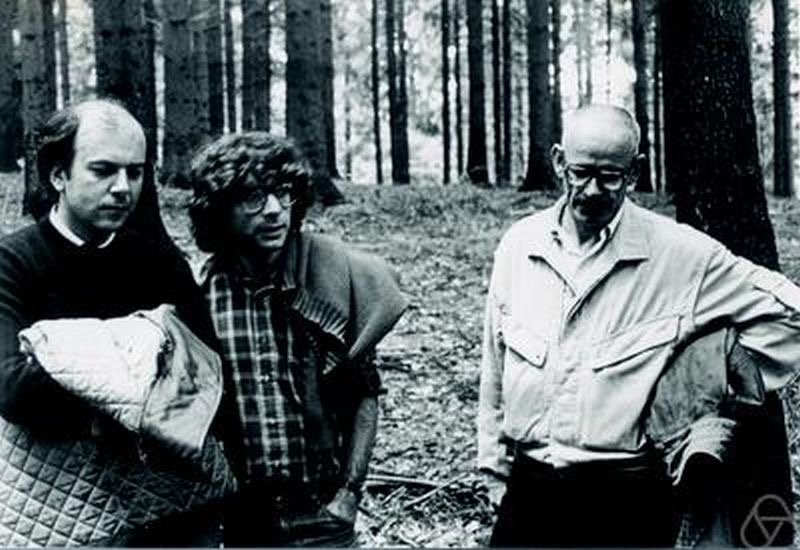
\includegraphics[width=14cm]{images/calogero.jpg}
\\ 
Francesco Calogero (a destra) con Corrado De Concini (a sinistra) e Eugene Trubowitz (al centro) a Oberwolfach nel 1984
\end{center}
\tableofcontents

\chapter[Oscillatore armonico ed eq. differenziali]{L'oscillatore armonico. Equazioni differenziali lineari a coefficienti costanti. Oscillazioni libere, smorzate, forzate, risonanze, transienti, equazioni differenziali lineari.}

\section{Premessa}

In questo capitolo discutiamo la equazione differenziale caratteristica dell'oscillatore armonico, e ne analizziamo le soluzioni. Accenniamo brevemente anche al caso più generale di equazione differenziale lineare a coefficienti costanti. Consideriamo infine il caso delle oscillazioni smorzate e quello delle oscillazioni forzate, e il fenomeno connesso della risonanza.

Poiché gli argomenti di questo capitolo dovrebbero essere già noti da corsi precedenti, la loro trattazione è alquanto rapida, avendo come scopo prevalente quello di richiamare nozioni già note.

Nell'ultimo paragrafo riportiamo i principali risultati della teoria delle equazioni differenziali lineari. 

\section{L'oscillatore armonico}

L'equazione caratteristica dell'oscillatore armonico è
\begin{equation}
    \ddot{x}(t) + \omega^2 x(t) = 0 \,.
\end{equation}
Qui, e generalmente nel seguito, il punto indica differenziazione rispetto alla variabile $t$. La costante $\omega$ ha evidentemente dimensioni $t^{-1}$, e prende il nome di \underline{pulsazione}.

La più generale soluzione della eq.~(1) si può scrivere
\begin{equation}
    x(t) = C \cos(\omega t) + S \sin(\omega t) \tag{2a}
\end{equation}
oppure
\begin{equation}
    x(t) = A \cos(\omega t + \varphi) \,, \tag{2b}
\end{equation}
le due espressioni essendo del tutto equivalenti con
\begin{equation}
    C = A \cos\varphi \,, \quad S = -A \sin\varphi \,.
\end{equation}
I valori delle costanti $C$ e $S$ (oppure $A$ e $\varphi$) risultano fissati una volta assegnate le \underline{condizioni iniziali}, cioè i valori della $x$ e della $\dot{x}$ ad un istante iniziale $t_0$:
\begin{equation}
    x(t_0) = a \,, \quad \dot{x}(t_0) = b \,.
\end{equation}
In forma esplicita:
\begin{align}
    A &= \left[ a^2 + (b/\omega)^2 \right]^{1/2} \,, \tag{5a} \\
    \varphi &= -\omega t_0 - \arctan\left[ b/(\omega a) \right] \,. \tag{5b}
\end{align}
Il moto descritto dalla (2) è periodico, con frequenza
\begin{equation}
    \nu = \frac{1}{T} = \frac{\omega}{2\pi} \,.
\end{equation}
È anzi il più semplice esempio di moto oscillatorio periodico.

La soluzione (2) può anche scriversi in forma esponenziale
\begin{equation}
    x(t) = B_+ e^{i\omega t} + B_- e^{-i\omega t} \,, \tag{2c}
\end{equation}
la condizione
\begin{equation}
    \left( B_+ \right)^* = B_-
\end{equation}
essendo necessaria e sufficiente affinché la $x(t)$ sia reale.

\begin{esercizi}
    \item Derivare le equazioni (5).
    \item Inventare tre modelli fisici che danno origine all'equazione del moto armonico, esprimere in ciascun caso la frequenza del moto in funzione delle grandezze fisiche caratteristiche di ciascun modello, e valutare numericamente il periodo di oscillazione corrispondente ad una scelta ragionevole dei valori di tali grandezze fisiche.
    \item Esprimere i parametri $B_+$ e $B_-$ della eq.~(2c) tramite i parametri $C$ ed $S$ della eq.~(2a), e verificare che la realtà di $C$ ed $S$ è necessaria e sufficiente per la validità della condizione (7). Si ricordi che
    \[
        e^{iz} = \cos z + i \sin z \,, \quad
        \cos z = \tfrac{1}{2}\left[ e^{iz} + e^{-iz} \right] \,, \quad
        \sin z = \tfrac{1}{2i}\left[ e^{iz} - e^{-iz} \right] \,.
    \]
\end{esercizi}

\section{Equazioni differenziali lineari a coefficienti costanti.}

La equazione dell'oscillatore armonico è un caso particolare di equazione differenziale lineare a coefficienti costanti. La più generale equazione di questo tipo si scrive
\begin{equation}
    \sum_{n=0}^{N} c_n \, x^{(n)}(t) = 0 \,,
\end{equation}
dove
\begin{equation}
    x^{(n)}(t) \equiv \frac{d^n x(t)}{d t^n} \,.
\end{equation}
L'oscillatore armonico è caratterizzato da
\begin{equation}
    N = 2 \,; \quad c_0 = \omega^2 \,, \quad c_1 = 0 \,, \quad c_2 = 1 \,.
\end{equation}

Come è immediato verificare, una soluzione delle eq.~(1) è data da
\begin{equation}
    x(t) = A \, e^{at}
\end{equation}
se $a$ è una soluzione della equazione algebrica
\begin{equation}
    \sum_{n=0}^{N} c_n \, a^n = 0 \,.
\end{equation}
Nel caso in cui questa equazione algebrica ammetta $N$ soluzioni distinte $a_n$, $n = 1, 2, \ldots, N$, la più generale soluzione delle eq.~(1) è
\begin{equation}
    x(t) = \sum_{n=1}^{N} A_n \, e^{a_n t} \,.
\end{equation}
Le $N$ costanti $A_n$ possono essere determinate se sono assegnate le condizioni iniziali, cioè se i valori della $x$ e delle sue derivate $x^{(n)}$ per $n = 1, 2, \ldots, N-1$ sono assegnati ad un certo istante (iniziale) $t_0$.

Si ricordi che la equazione algebrica (5) ammette al più $N$ soluzioni distinte, e che, se le costanti $c_n$ sono reali, queste soluzioni $a_n$ sono reali oppure compaiono a coppie complesse coniugate (infatti se una $a$ complessa è soluzione delle (5), anche la complessa coniugata $a^*$ è necessariamente soluzione, come si vede considerando la equazione complessa coniugata della (5)).

Naturalmente se le $N+1$ costanti $c_n$ sono reali, e le condizioni iniziali sono reali, la soluzione $x(t)$ della equazione differenziale (1) risulta anche reale (anche se le radici $a_n$ non sono tutte reali!). In generale la parte reale delle $a_n$ dà origine ad andamenti esponenziali, la parte immaginaria ad andamenti oscillanti. La soluzione è puramente oscillante se tutte le $a_n$ sono immaginarie pure; altrimenti generalmente, per $t \to \infty$, la soluzione tende a zero o diverge. Le soluzioni sono periodiche se tutte le $a_n$ sono immaginarie pure, ed inoltre sono tutte fra loro commensurabili, cioè se i rapporti $a_n / a_m$ sono tutti numeri razionali. Si noti che queste proprietà dipendono solo dalla struttura della equazione differenziale (1) (cioè dai valori di $N$ e degli $N+1$ coefficienti $c_n$), e non dalle condizioni iniziali.

Ricordiamo infine che molte delle affermazioni di questo paragrafo sono valide purché non si verifichi il caso eccezionale che la equazione algebrica (5) ammetta meno di $N$ soluzioni distinte (ovvero, che due o più delle $N$ soluzioni $a_n$ delle (5) coincidano fra loro).

\begin{esercizi}
    \item Scrivere la soluzione della equazione differenziale
    \[
        \dddot{x}(t) + 2\ddot{x}(t) + 10\dot{x}(t) = 0 \,,
    \]
    con condizioni iniziali
    \[
        x(0) = 0 \,, \quad \dot{x}(0) = 10 \,, \quad \ddot{x}(0) = -10 \,.
    \]
    \item Dimostrare tutte le affermazioni contenute nel testo di questa sezione.
    \item[*] Quali delle affermazioni ed equazioni contenute in questa sezione non sono più valide se due o più $a_n$ coincidono fra loro? E come vanno modificate?
\end{esercizi}

\section[EDO secondo ordine a coeff. costanti]{La equazione differenziale lineare omogenea del secondo ordine a coefficienti costanti. Andamento oscillante ed esponenziale della soluzione.}

Studiamo più in dettaglio il caso $N = 2$ (equazione differenziale del secondo ordine):
\begin{equation}
    c_2 \ddot{x}(t) + c_1 \dot{x}(t) + c_0 x(t) = 0 \,,
\end{equation}
supponendo per semplicità che i coefficienti $c_n$ siano reali. La equazione algebrica associata,
\begin{equation}
    c_2 a^2 + c_1 a + c_0 = 0 \,,
\end{equation}
ammette le due soluzioni
\begin{equation}
    a = \alpha \pm \beta \,,
\end{equation}
con
\begin{align}
    \alpha &= -\frac{1}{2}\frac{c_1}{c_2} \,, \tag{4} \\
    \beta^2 &= (c_1^2 - 4 c_0 c_2) / (4 c_2^2) \,. \tag{5}
\end{align}

\subsubsection*{Primo caso: $\beta^2 > 0$.}

Allora $\beta$ è reale (e per convenzione lo scegliamo positivo). La soluzione ha andamento esponenziale:
\begin{equation}
    x(t) = e^{\alpha t} \left[ B_+ e^{\beta t} + B_- e^{-\beta t} \right] \,.
\end{equation}
Per $t \to \infty$ la $x(t)$ diverge esponenzialmente se $\alpha > \beta$, e si annulla esponenzialmente se $\alpha < -\beta$; queste conclusioni sono indipendenti dalle condizioni iniziali. Se invece $-\beta < \alpha < \beta$, $x(t)$ per $t \to \infty$ generalmente diverge, salvo per quelle speciali scelte di condizioni iniziali che corrispondono a $B_+ = 0$ nella (6).

\subsubsection*{Secondo caso: $\beta^2 < 0$.}

Allora $\beta$ è immaginario puro, sicché conviene porre
\begin{equation}
    \beta = i\omega
\end{equation}

% continuazione sezione 1.3

con $\omega$ reale (positivo per convenzione). La soluzione si può scrivere
\begin{equation}
    x(t) = e^{\alpha t} \left[ C \cos(\omega t) + S \sin(\omega t) \right] .
\end{equation}
Se $\alpha = 0$ le soluzioni sono oscillanti, anzi periodiche; in effetti,
$\alpha = 0$ si può avere solo per $c_1 = 0$, nel qual caso si torna dunque
al caso dell'oscillatore armonico discusso in 1.1 (con $\omega = (c_0/c_2)^{1/2}$).
Se $\alpha \neq 0$, si ha un moto oscillatorio di pulsazione $\omega$, la cui ampiezza
però cresce (se $\alpha > 0$) o cala (se $\alpha < 0$) esponenzialmente col
tempo. Si noti che la scelta fra le due alternative dipende solo dal segno di
$\alpha$, ovvero dal segno relativo di $c_0$ e $c_2$, e non dalle condizioni iniziali
(che fissano i valori delle costanti $C$ ed $S$). Nel caso $\alpha < 0$, si parla
di moto oscillatorio smorzato, e ad $\alpha$ si dà il nome di \underline{coefficiente di smorzamento}.

\subsubsection*{Terzo caso: $\beta = 0$.}

Si hanno allora 2 soluzioni coincidenti della equazione algebrica (2). Siamo
dunque nel caso eccezionale menzionato al capitolo precedente. La soluzione,
come è facile verificare, è
\begin{equation}
    x(t) = (A + B t) \, e^{\alpha t} \,,
\end{equation}
con $A$ e $B$ costanti che vengono fissate dalle condizioni iniziali. La presenza
di un polinomio a moltiplicare (in questo caso, di primo grado) è per l'appunto
caratteristica del caso in cui si abbiano soluzioni coincidenti della equazione
algebrica associata alla equazione differenziale (anche nel caso $N > 2$).

Questi stessi risultati si sarebbero potuti ottenere trasformando la (1) in
forma canonica, con la posizione
\begin{equation}
    x(t) = e^{\alpha t} \, y(t) \,.
\end{equation}
Infatti si ottiene allora per la $y(t)$ la equazione differenziale
\begin{equation}
    \ddot{y}(t) - \beta^2 \, y(t) = 0 \,,
\end{equation}
che ammette la soluzione
\begin{equation}
    y(t) = B_+ e^{\beta t} + B_- e^{-\beta t} \,. \tag{12}
\end{equation}
Naturalmente se $\beta^2 < 0$, invece della (12) potremo scrivere
\begin{equation}
    y(t) = C \cos(\omega t) + S \sin(\omega t) \,, \tag{13}
\end{equation}
con $\omega$ dato dalla (7); laddove, se $\beta = 0$, chiaramente la soluzione della (11) è
\begin{equation}
    y(t) = A + B t \,. \tag{14}
\end{equation}

\begin{esercizi}
    \item Trovare in forma esplicita le soluzioni delle seguenti equazioni
    differenziali, con le condizioni iniziali indicate in ciascun caso:
\begin{enumerate}
        \item $\tfrac{1}{2}\ddot{x}(t) + \dot{x}(t) + 13x(t) = 0$,\quad $x(0)=0$, $\dot{x}(0)=5$
        \item \phantom{$\tfrac{1}{2}\ddot{x}(t) + \dot{x}(t) + 13x(t) = 0$,}\quad $x(0)=2$, $\dot{x}(0)=3$
        \item \phantom{$\tfrac{1}{2}\ddot{x}(t) + \dot{x}(t) + 13x(t) = 0$,}\quad $x(0)=5$, $\dot{x}(0)=0$
        \item $\tfrac{1}{2}\ddot{x}(t) - \dot{x}(t) + 13x(t) = 0$,\quad $x(0)=0$, $\dot{x}(0)=5$
        \item \phantom{$\tfrac{1}{2}\ddot{x}(t) - \dot{x}(t) + 13x(t) = 0$,}\quad $x(0)=2$, $\dot{x}(0)=3$
        \item \phantom{$\tfrac{1}{2}\ddot{x}(t) - \dot{x}(t) + 13x(t) = 0$,}\quad $x(0)=5$, $\dot{x}(0)=0$
        \item $\ddot{x}(t) + 2\dot{x}(t) - 3x(t) = 0$,\quad $x(0)=0$, $\dot{x}(0)=4$
        \item \phantom{$\ddot{x}(t) + 2\dot{x}(t) - 3x(t) = 0$,}\quad $x(0)=1$, $\dot{x}(0)=-2$
        \item \phantom{$\ddot{x}(t) + 2\dot{x}(t) - 3x(t) = 0$,}\quad $x(0)=1$, $\dot{x}(0)=-3$
        \item \phantom{$\ddot{x}(t) + 2\dot{x}(t) - 3x(t) = 0$,}\quad $x(0)=1$, $\dot{x}(0)=-4$
        \item $\ddot{x}(t) + 2\dot{x}(t) + x(t) = 0$,\quad $x(0)=1$, $\dot{x}(0)=-1$
        \item \phantom{$\ddot{x}(t) + 2\dot{x}(t) + x(t) = 0$,}\quad $x(0)=0$, $\dot{x}(0)=-1$
        \item \phantom{$\ddot{x}(t) + 2\dot{x}(t) + x(t) = 0$,}\quad $x(0)=1$, $\dot{x}(0)=-2$
    \end{enumerate}
    \item Graficare su carta millimetrata o quadrettata le soluzioni
    dell'esercizio precedente, e confrontare fra loro sia le soluzioni della
    stessa equazione con diverse condizioni al contorno, che le soluzioni di
    equazioni diverse.
    \item Quali sono i possibili comportamenti asintotici della $x(t)$ se
    $\alpha = \pm\beta$? È possibile che si verifichi questa eventualità se
    $c_1 \neq 0$? ($\alpha$ e $\beta$ definiti dalle eq.~(4) e (5).)
    \item Studiare le piccole oscillazioni di un pendolo in un mezzo viscoso
    (schematizzando l'attrito come una forza di modulo proporzionale alla
    velocità).
\end{esercizi}

\section[edo secondo ordine lineare a coeff. costanti non omogenea]{La equazione differenziale lineare del secondo ordine a coefficienti costanti non omogenea.}

Finora abbiamo considerato equazioni omogenee. Ora passiamo a studiare la
equazione differenziale lineare del secondo ordine a coefficienti costanti non
omogenea, che scriviamo
\begin{equation}
    c_2 \ddot{x}(t) + c_1 \dot{x}(t) + c_0 x(t) = f(t) \,.
\end{equation}
Al termine $f(t)$ si dà il nome di \underline{termine noto}. Nel seguito supporremo
sempre, per semplicità, che la funzione $f(t)$ esista e sia finita per ogni $t$ finito.

La equazione (3.1), che si ottiene ponendo a zero il termine noto nella (1),
prende il nome di \underline{equazione omogenea associata}.

Prima di procedere oltre, conviene trasformare la (1) in forma canonica,
ponendo
\begin{equation}
    x(t) = e^{\alpha t} \, y(t)
\end{equation}
con
\begin{equation}
    \alpha = -c_1 / (2 c_2)
\end{equation}
come nella sezione precedente. Si ottiene allora per la $y(t)$ la equazione
\begin{equation}
    \ddot{y}(t) - \beta^2 \, y(t) = g(t)
\end{equation}
con
\begin{equation}
    g(t) = e^{-\alpha t} f(t) / c_2
\end{equation}
e $\beta^2$ definito, come nel paragrafo precedente, da
\begin{equation}
    \beta^2 = (c_1^2 - 4 c_0 c_2) / (4 c_2^2) \,.
\end{equation}
È facile verificare che una soluzione della (4) è data da
\begin{equation}
    y(t) = (2\beta)^{-1} \int_{\bar{t}}^{t} dt' \left\{ e^{\beta(t-t')} - e^{-\beta(t-t')} \right\} g(t') \,.
\end{equation}
Infatti, differenziando si ottiene
\begin{equation}
    \dot{y}(t) = \frac{1}{2} \int_{\bar{t}}^{t} dt' \left\{ e^{\beta(t-t')} + e^{-\beta(t-t')} \right\} g(t')
\end{equation}
(si noti che il termine ottenuto differenziando il limite superiore di integrazione
si annulla). Differenziando ancora
\begin{align}
    \ddot{y}(t) &= \frac{1}{2} \beta \int_{\bar{t}}^{t} dt' \left\{ e^{\beta(t-t')} - e^{-\beta(t-t')} \right\} g(t') + g(t) \tag{9a} \\
    &= \beta^2 y(t) + g(t) \tag{9b}
\end{align}
come volevasi dimostrare.

La soluzione più generale della (4) si ottiene aggiungendo alla (7) la più
generale soluzione della equazione omogenea associata alla (4):
\begin{equation}
    \ddot{Y}(t) - \beta^2 Y(t) = 0 \,.
\end{equation}
È infatti evidente che se $y(t)$ è soluzione della (4), $y(t) + Y(t)$ è ancora
soluzione della stessa equazione (per verificare basta sommare la (4) e la
(10)). Scriveremo dunque:
\begin{align}
    y(t) &= B_+ e^{\beta t} + B_- e^{-\beta t} + \notag \\
    &\quad + (2\beta)^{-1} \int_{\bar{t}}^{t} dt' \left\{ e^{\beta(t-t')} - e^{-\beta(t-t')} \right\} g(t') \,. \tag{11}
\end{align}
Apparentemente questa soluzione contiene 3 costanti arbitrarie ($B_+$, $B_-$ e
$\bar{t}$); ma è facile convincersi che ve ne sono solo 2 indipendenti. Infatti un
cambiamento di $\bar{t}$ (da $\bar{t}$ a $\tilde{t}$) equivale ad aggiungere alla soluzione il
pezzo
\begin{equation}
    (2\beta)^{-1} \int_{\bar{t}}^{\tilde{t}} dt' \left\{ e^{\beta(t-t')} - e^{-\beta(t-t')} \right\} g(t') =
    \bar{B}_+ e^{\beta t} + \bar{B}_- e^{-\beta t} \tag{12}
\end{equation}
con
\begin{equation}
    \bar{B}_\pm = \pm (2\beta)^{-1} \int_{\tilde{t}}^{\bar{t}} dt' \, e^{\mp \beta t'} \, g(t') \,, \tag{13}
\end{equation}
ed è dunque del tutto equivalente ad un cambiamento delle due costanti $B_+$ e
$B_-$, e precisamente alla aggiunta di $\bar{B}_+$ a $B_+$ e $\bar{B}_-$ a $B_-$.

Nel caso in cui $\beta^2$ sia negativo, e dunque $\beta$ immaginario puro, la
soluzione (11) è naturalmente ancora valida; può anche essere riscritta in
forma reale ponendo, come al solito,
\begin{equation}
    \beta = i\omega \,, \tag{14}
\end{equation}
e scrivendo
\begin{equation}
    y(t) = C \cos(\omega t) + S \sin(\omega t) + \omega^{-1} \int_{\bar{t}}^{t} dt' \, \sin[\omega(t-t')] \, g(t') \,. \tag{15}
\end{equation}
Combinando le formule (2), (5) e (11) o (15) possiamo in conclusione scrivere,
per la più generale soluzione della equazione (1),
\begin{align}
    x(t) &= e^{\alpha t} \left[ B_+ e^{\beta t} + B_- e^{-\beta t} \right] + \notag \\
    &\quad + (2\beta c_2)^{-1} \int_{\bar{t}}^{t} dt' \left\{ e^{\beta(t-t')} - e^{-\beta(t-t')} \right\} \cdot \notag \\
    &\quad \cdot e^{\alpha(t-t')} f(t') \tag{16}
\end{align}
oppure
\begin{align}
    x(t) &= e^{\alpha t} \left[ C \cos(\omega t) + S \sin(\omega t) \right] + \notag \\
    &\quad + (\omega c_2)^{-1} \int_{\bar{t}}^{t} dt' \, \sin[\omega(t-t')] \, e^{\alpha(t-t')} f(t') \,, \tag{17}
\end{align}
con $\alpha$, $\beta$ ed $\omega$ definiti dalle eq.~(3), (6) e (14).

Le costanti $B_+$ e $B_-$, o $C$ ed $S$, vengono generalmente determinate dalle
condizioni iniziali
\begin{equation}
    x(t_0) = a \,, \quad \dot{x}(t_0) = b \,, \tag{18}
\end{equation}
dopo che è stato scelto, a priori arbitrariamente, il valore della costante $\bar{t}$.
Una scelta conveniente è
\begin{equation}
    \bar{t} = t_0 \,, \tag{19}
\end{equation}
perché allora le costanti $B_+$ e $B_-$, o $C$ ed $S$, risultano legate alle condizioni
iniziali (18) dalle semplici relazioni
\begin{align}
    a &= e^{\alpha t_0} \left[ B_+ e^{\beta t_0} + B_- e^{-\beta t_0} \right] \tag{20a} \\
    b &= \alpha a + \beta \, e^{\alpha t_0} \left[ B_+ e^{\beta t_0} - B_- e^{-\beta t_0} \right] \tag{20b}
\end{align}
ovvero
\begin{align}
    a &= e^{\alpha t_0} \left[ C \cos(\omega t_0) + S \sin(\omega t_0) \right] \tag{21a} \\
    b &= \alpha a + \omega \, e^{\alpha t_0} \left[ -C \sin(\omega t_0) + S \cos(\omega t_0) \right] \tag{21b}
\end{align}
la cui esplicita soluzione è
\begin{align}
    B_+ &= (2\beta)^{-1} \left[ b + (\beta - \alpha) a \right] e^{-(\alpha+\beta)t_0} \tag{22a} \\
    B_- &= (2\beta)^{-1} \left[ -b + (\beta+\alpha) a \right] e^{-(\alpha-\beta)t_0} \tag{22b}
\end{align}
ovvero
\begin{align}
    C &= \omega^{-1} \left[ \omega a \cos(\omega t_0) - (b - \alpha a) \sin(\omega t_0) \right] e^{-\alpha t_0} \tag{23a} \\
    S &= \omega^{-1} \left[ \omega a \sin(\omega t_0) + (b - \alpha a) \cos(\omega t_0) \right] e^{-\alpha t_0} \,. \tag{23b}
\end{align}
Queste relazioni diventano particolarmente semplici se $t_0 = 0$, nel qual caso
\begin{align}
    B_+ &= (2\beta)^{-1} \left[ b + (\beta - \alpha) a \right] \tag{24a} \\
    B_- &= (2\beta)^{-1} \left[ -b + (\beta + \alpha) a \right] \tag{24b}
\end{align}
ovvero
\begin{align}
    C &= a \tag{25a} \\
    S &= (b - \alpha a)/\omega \,. \tag{25b}
\end{align}

\begin{esercizi}
    \item Determinare per $t > 0$ la funzione $x(t)$ definita dalla eq.~differenziale
    \[
        5\ddot{x}(t) + 6\dot{x}(t) + x(t) = 4 e^{-t}
    \]
    e dalle condizioni al contorno $x(0) = 0$, $\dot{x}(0) = 1$.
    \item La funzione $x(t)$ è definita dalla equazione differenziale
    \[
        \ddot{x}(t) + 4\dot{x}(t) - 5x(t) = 18 \, e^{-2t}
    \]
    con condizioni al contorno $x(0) = a$, $\dot{x}(0) = 0$.
    Determinare l'intervallo di valori di $a$ per cui la $x(t)$ per $t > 0$
    cambia segno; e, per $a$ entro tale intervallo, determinare la funzione
    $\bar{t}(a)$, con $\bar{t}$ definito da $x(\bar{t}) = 0$.
    \item Ottenere, dalla equazione (16) e seguenti (o (17) e seguenti), le
    formule per il caso in cui $\beta$ (ovvero $\omega$) si annulla, cioè per il caso
    in cui le due radici della equazione algebrica (3.2) coincidono; e
    verificare che danno la soluzione generale della equazione (1) nel caso
    in questione.
    \item Determinare per $t > 0$ la funzione $x(t)$ definita dalla equazione
    differenziale
    \[
        2\ddot{x}(t) + 4\dot{x}(t) + 10 x(t) = e^{-t} - e^{-2t}
    \]
    con condizioni al contorno $x(0) = \dot{x}(0) = 0$.
    Si annulla o no questa funzione per $t > 0$?
    \item La funzione $x(t)$ è definita dalla equazione differenziale
    \[
        3\ddot{x}(t) + 7\dot{x}(t) - A \, x(t) = 5 - 4 e^{-t}
    \]
    con condizioni al contorno $x(0) = 0$, $\dot{x}(0) = 0$.
    È possibile scegliere un valore positivo della costante $A$, per cui la
    $x(t)$ si annulli per $t > 0$?
    \item La funzione $x(t)$ è definita dalla equazione differenziale
    \[
        c_2 \ddot{x}(t) + c_1 \dot{x}(t) + c_0 x(t) = A + Bt
    \]
    con $c_0 \neq 0$. Dimostrare che, se $\alpha < |\operatorname{Re}\beta|$, con
    $\alpha = -c_1/(2c_2)$, $\beta^2 = (c_1^2 - 4c_0 c_2)/(4c_2^2)$, qualunque
    siano le condizioni iniziali e i valori di $A$ e $B$ (purché non ambedue
    nulli),
    \[
        \lim_{t \to \infty} \left[ x(t) / \Xi(t) \right] = 1
    \]
    con
    \[
        \Xi(t) = \left[ (A - c_1 B) / c_0 \right] + B t \,.
    \]
    \item[*] Dimostrare che la soluzione generale della equazione
    \[
        c_2 \ddot{x}(t) + c_1 \dot{x}(t) + c_0 x(t) = \sum_{n=0}^{N} a_n t^n
    \]
    con $c_0 \neq 0$, è
    \begin{align*}
        x(t) &= e^{\alpha t} \left[ B_+ e^{\beta t} + B_- e^{-\beta t} \right] + \\
        &\quad + (a_N/c_0) \, t^N + \left[ (a_{N-1}/c_0) - (c_1 N a_N / c_0^2) \right] t^{N-1} + \\
        &\quad + P_{N-2}(t) \,,
    \end{align*}
    con $\alpha$ e $\beta$ dati dalle eq.~(3) e (6), $B_+$ e $B_-$ costanti arbitrarie,
    e $P_{N-2}(t)$ polinomio di grado $N-2$.
    \item Trovare le condizioni necessarie e sufficienti affinché, qualunque
    siano le condizioni iniziali, la soluzione della equazione differenziale
    \[
        c_2 \ddot{x}(t) + c_1 \dot{x}(t) + c_0 x(t) = A \, e^{\gamma t}
    \]
    abbia la struttura
    \[
        x(t) = e^{\alpha t} \left[ B_+ e^{\beta t} + B_- e^{-\beta t} \right] + C \, e^{\gamma t}
    \]
    con $B_+$, $B_-$ e $C$ costanti.
\end{esercizi}

\section{Sorgente sinusoidale. Risonanza}

È interessante discutere il problema in cui le soluzioni della equazione
omogenea sono periodiche, ed anche il termine noto è periodico. Consideriamo
dunque la equazione differenziale
\begin{equation}
    c_2 \ddot{x}(t) + c_1 \dot{x}(t) + c_0 x(t) = A \sin(\Omega t + \phi) \,.
\end{equation}
Supponendo che sia positivo
\begin{equation}
    \omega^2 = (4 c_0 c_2 - c_1^2) / (4 c_2^2) \,,
\end{equation}
e indicando come al solito con $\alpha$ il coefficiente di smorzamento,
$\alpha = -c_1/(2c_2)$, otteniamo per la più generale soluzione della (1) la
espressione
\begin{align}
    x(t) &= e^{\alpha t} \left[ \bar{C} \cos(\omega t) + \bar{S} \sin(\omega t) \right] + \notag \\
    &\quad + \left[ A/(\omega c_2) \right] \int_0^t dt' \, \sin[\omega(t-t')] \, e^{\alpha(t-t')} \sin(\Omega t' + \phi) \,. \tag{3}
\end{align}
Effettuando esplicitamente la integrazione otteniamo
\begin{align}
    x(t) &= e^{\alpha t} \left[ C \cos(\omega t) + S \sin(\omega t) \right] + \notag \\
    &\quad + \left[ A / c_2 \right] \left\{ \left[ \alpha^2 + (\omega+\Omega)^2 \right] \left[ \alpha^2 + (\omega-\Omega)^2 \right] \right\}^{-1} \notag \\
    &\quad \cdot \left\{ 2\Omega\alpha \cos(\Omega t+\phi) - (\alpha^2 + \Omega^2 - \omega^2) \sin(\Omega t + \phi) \right\} \,, \tag{5}
\end{align}
con $C$, $S$ nuove costanti (sempre arbitrarie).

\bigskip
\noindent\rule{\textwidth}{0.4pt}
\begin{small}
Un metodo conveniente per effettuare l'integrale
\[
    I = \int_0^t dt' \, \sin[\omega(t-t')] \, e^{\alpha(t-t')} \sin(\Omega t' + \phi)
\]
utilizza le formule di prostaferesi, secondo cui
\[
    \sin A \sin B = \tfrac{1}{2} \left[ \cos(A-B) - \cos(A+B) \right]
\]
e la formula
\[
    e^{ix} = \cos x + i \sin x
\]
che implica
\[
    \cos x = \operatorname{Re} e^{ix}
\]
dove il simbolo Re indica la parte reale. In tal modo
\begin{align*}
    I &= \frac{1}{2} \int_0^t dt' \, e^{\alpha(t-t')} \left\{ \cos[\omega(t-t') - \Omega t' - \phi] - \cos[\omega(t-t') + \Omega t' + \phi] \right\} \\
    &= \frac{1}{2} \operatorname{Re} \int_0^t dt' \left\{ e^{[(\alpha+i\omega)(t-t')-i\Omega t'-i\phi]} + e^{[(\alpha+i\omega)(t-t')+i\Omega t'+i\phi]} \right\} \\
    &= \frac{1}{2} \operatorname{Re} \left\{ -[\alpha+i(\omega+\Omega)]^{-1} \left[ e^{-i\Omega t - i\phi} - e^{(\alpha+i\omega)t - i\phi} \right] + \right. \\
    &\qquad \left. + [\alpha+i(\omega-\Omega)]^{-1} \left[ e^{i\Omega t + i\phi} - e^{(\alpha+i\omega)t + i\phi} \right] \right\} \\
    &= \frac{1}{2} \left\{ - [\alpha^2+(\omega+\Omega)^2]^{-1} \left[ \alpha[\cos(\Omega t+\phi) - e^{\alpha t}\cos(\omega t-\phi)] \right. \right. \\
    &\qquad \left. - (\omega+\Omega)[\sin(\Omega t+\phi) - e^{\alpha t}\sin(\omega t-\phi)] \right] + \\
    &\qquad + [\alpha^2+(\omega-\Omega)^2]^{-1} \left[ \alpha[\cos(\Omega t+\phi) - e^{\alpha t}\cos(\omega t+\phi)] \right. \\
    &\qquad \left. \left. + (\omega-\Omega)[\sin(\Omega t+\phi) - e^{\alpha t}\sin(\omega t+\phi)] \right] \right\} \\
    &= \left\{ [\alpha^2+(\omega+\Omega)^2][\alpha^2+(\omega-\Omega)^2] \right\}^{-1} \omega \\
    &\quad \cdot \left\{ 2\Omega\alpha\cos(\Omega t+\phi) - (\alpha^2+\Omega^2-\omega^2)\sin(\Omega t+\phi) \right\} + \\
    &\quad + e^{\alpha t} \left[ C' \cos(\omega t) + S' \sin(\omega t) \right]
\end{align*}
con $C'$ ed $S'$ risultando espresse in funzione di $\alpha$, $\omega$, $\Omega$ e $\phi$.
\end{small}
\noindent\rule{\textwidth}{0.4pt}
\bigskip

La soluzione (5) contiene dunque, come al solito, una parte caratteristica del
moto proprio del sistema (la soluzione della equazione omogenea) e una parte
indotta dal termine noto, che risulta essere di nuovo una funzione sinusoidale
con la stessa frequenza del termine noto (ma con diversa fase, se $\alpha \neq 0$).

Il caso $\alpha = 0$ è particolarmente interessante. In questo caso, in cui la
parte omogenea della equazione (1) si riduce a quella del moto armonico, la
soluzione (5) diventa
\begin{align}
    x(t) &= C \cos(\omega t) + S \sin(\omega t) + \notag \\
    &\quad + \left[ A / c_2 \right] (\omega^2 - \Omega^2)^{-1} \sin(\Omega t + \phi) \,. \tag{6}
\end{align}
Conviene riscrivere questa equazione nella forma
\begin{align}
    x(t) &= \tilde{C} \cos(\omega t) + \tilde{S} \sin(\omega t) + \notag \\
    &\quad + \left[ A / c_2 \right] (\omega^2 - \Omega^2)^{-1} \left[ \sin(\Omega t+\phi) - \sin(\omega t+\phi) \right] \,, \tag{7}
\end{align}
che è del tutto equivalente alla precedente se
\begin{align}
    \tilde{C} &= C + \left[ A / c_2 \right] (\omega^2-\Omega^2)^{-1} \sin\phi \,, \tag{8a} \\
    \tilde{S} &= S + \left[ A / c_2 \right] (\omega^2-\Omega^2)^{-1} \cos\phi \,. \tag{8b}
\end{align}
Le nuove costanti $\tilde{C}$ ed $\tilde{S}$ sono naturalmente sempre arbitrarie, finché
non siano fissate dalle condizioni iniziali. Usando inoltre l'identità
trigonometrica
\[
    \sin A - \sin B = 2 \sin\left[\tfrac{1}{2}(A-B)\right] \cos\left[\tfrac{1}{2}(A+B)\right]
\]
si scrive
\begin{align}
    x(t) &= \tilde{C} \cos(\omega t) + \tilde{S} \sin(\omega t) + \notag \\
    &\quad + \left[ A / c_2 \right] (\omega^2-\Omega^2)^{-1} \, 2 \sin\left[\tfrac{1}{2}(\Omega-\omega)t\right] \cos\left[\tfrac{1}{2}(\omega+\Omega)t+\phi\right] \,. \tag{9}
\end{align}
Questa espressione è particolarmente conveniente per studiare il caso in cui la
pulsazione $\Omega$ del termine noto coincide con la pulsazione propria del sistema
$\omega$. In tal caso
\begin{align}
    x(t) &= \tilde{C} \cos(\omega t) + \tilde{S} \sin(\omega t) \notag \\
    &\quad - \left[ A/(2\omega c_2) \right] t \, \cos(\omega t + \phi) \,. \tag{10}
\end{align}
Dunque in questo caso particolare la soluzione contiene una parte che oscilla
con frequenza $\omega$, con un ritardo di fase $\frac{\pi}{2}$ rispetto al termine noto, e
con una ampiezza che cresce linearmente nel tempo. È questo il fenomeno della
\underline{risonanza}.

\begin{esercizi}
    \item Derivare esplicitamente le costanti $C'$ ed $S'$, sostituire nella (5)
    $C = \tilde{C} + C'$ e $S = \tilde{S} + S'$, e ponendo $\alpha=0$, $\omega=\Omega$, riottenere
    la (10).
    \item Dimostrare direttamente che nel caso $c_1 = 0$, $\Omega = \omega$, la
    espressione $-[A/(2\omega c_2)] \, t \, \cos(\omega t + \phi)$ è una soluzione
    particolare della (1).
\end{esercizi}

\section{Termine noto ``transiente''. Condizioni asintotiche.}

Consideriamo la solita equazione differenziale
\begin{equation}
    c_2 \ddot{x}(t) + c_1 \dot{x}(t) + c_0 x(t) = f(t) \,,
\end{equation}
e supponiamo che il termine noto si annulli asintoticamente per $|t| \to \infty$,
più rapidamente di $1/t$. (Più precisamente: supponiamo che esista un numero
$\varepsilon$ positivo tale che
\begin{equation}
    \lim_{|t| \to \infty} \left[ t^{1+\varepsilon} f(t) \right] = 0 \,, \quad \varepsilon > 0 \,. \tag{2}
\end{equation}
)

È allora facile vedere che, per ogni soluzione $x(t)$, esistono due soluzioni
$y_+(t)$ e $y_-(t)$ della equazione omogenea associata, tali che
\begin{align}
    \lim_{t \to +\infty} \left[ x(t) - y_+(t) \right] &= 0 \,, \tag{3} \\
    \lim_{t \to -\infty} \left[ x(t) - y_-(t) \right] &= 0 \,. \tag{4}
\end{align}
È dunque possibile individuare una particolare soluzione $x(t)$, anziché
fissando il suo valore e quello della sua derivata per un certo valore $t_0$
della variabile $t$, imponendo che essa coincida con una data soluzione della
equazione omogenea per $t \to -\infty$ (oppure per $t \to +\infty$). Questo tipo
di problema si presenta in molti casi di interesse fisico, specialmente per
valori dei parametri $c_0$, $c_1$ e $c_2$ tali che la soluzione della equazione
omogenea associata alla (1) è oscillante ($c_1 = 0$, $c_0/c_2 > 0$), nel qual caso
il limite della $x(t)$ per grandi $t$ generalmente non esiste (la funzione oscilla).

Fissiamo dunque l'attenzione sull'equazione del moto armonico:
\begin{equation}
    \ddot{x}(t) + \omega^2 x(t) = g(t)
\end{equation}
e supponiamo di voler determinare la soluzione di questa equazione caratterizzata
dalla condizione asintotica
\begin{equation}
    \lim_{t \to -\infty} \left\{ x(t) - \left[ C \cos(\omega t) + S \sin(\omega t) \right] \right\} = 0 \,. \tag{6}
\end{equation}
È facile verificare che questa soluzione è data dalla formula
\begin{align}
    x(t) &= C \cos(\omega t) + S \sin(\omega t) + \notag \\
    &\quad + \omega^{-1} \int_{-\infty}^{t} dt' \, \sin[\omega(t-t')] \, g(t') \,, \tag{7}
\end{align}
l'integrazione risultando convergente grazie alla ipotesi
\begin{equation}
    \lim_{t \to -\infty} \left[ t^{1+\varepsilon} g(t) \right] = 0 \,, \quad \varepsilon > 0 \,. \tag{8}
\end{equation}
Se inoltre
\begin{equation}
    \lim_{t \to +\infty} \left[ t^{1+\varepsilon'} g(t) \right] = 0 \,, \quad \varepsilon' > 0 \,, \tag{9}
\end{equation}
allora è facile dimostrare che
\begin{equation}
    \lim_{t \to +\infty} \left\{ x(t) - \left[ C' \cos(\omega t) + S' \sin(\omega t) \right] \right\} = 0 \,, \tag{10}
\end{equation}
con
\begin{align}
    C' &= C - \omega^{-1} \int_{-\infty}^{+\infty} dt \, \sin(\omega t) \, g(t) \,, \tag{11a} \\
    S' &= S + \omega^{-1} \int_{-\infty}^{+\infty} dt \, \cos(\omega t) \, g(t) \,. \tag{11b}
\end{align}

\noindent\rule{\textwidth}{0.4pt}
\subsubsection*{Dimostrazione}

Dalle (7) e (11) segue
\[
    x(t) - \left[ C' \cos(\omega t) + S' \sin(\omega t) \right] = -\omega^{-1} \int_t^{\infty} dt' \, \sin[\omega(t-t')] \, g(t') \,.
\]
Da questa segue
\[
    \left| x(t) - \left[ C' \cos(\omega t) + S' \sin(\omega t) \right] \right| < \omega^{-1} \int_t^{\infty} dt' \, |g(t')| \,.
\]
Ma la condizione (9) implica che, per $t$ sufficientemente grande, esistono
costanti positive $A$ ed $\varepsilon$ tali che
\[
    |g(t)| < A \, t^{-(1+\varepsilon)} \,, \quad \varepsilon > 0 \,.
\]
Pertanto, per $t$ sufficientemente grande,
\[
    \left| x(t) - \left[ C' \cos(\omega t) + S' \sin(\omega t) \right] \right| < \left[ A/(\omega\varepsilon) \right] t^{-\varepsilon} \,, \quad \varepsilon > 0 \,,
\]
da cui segue la (10), c.v.d.
\noindent\rule{\textwidth}{0.4pt}

\begin{esercizi}
    \item Dimostrare che la soluzione (7) della equazione differenziale (5)
    soddisfa alla condizione (6).
    \item La funzione $x(t)$ è soluzione della equazione differenziale (5), ed
    è caratterizzata dalla condizione asintotica
    \[
        \lim_{t \to -\infty} \left[ x(t) \, e^{-i\omega t} \right] = 1 \,.
    \]
    Calcolare la $x(t)$ e valutarne l'andamento per $t \to +\infty$.
    \item La funzione $x(t)$ è soluzione della equazione differenziale
    \[
        \ddot{x}(t) + 9 x(t) = \Theta(t) \left[ e^{-t} - e^{-3t} \right]
    \]
    con $\Theta(t) = 0$ per $t < 0$, $\Theta(t) = 1$ per $t \geq 0$, ed è
    caratterizzata dalla condizione asintotica
    \[
        \lim_{t \to -\infty} \left[ x(t) - \sin(3t) \right] = 0 \,.
    \]
    Calcolare la $x(t)$.
    \item La funzione $x(t)$ è soluzione della equazione differenziale
    \[
        \ddot{x}(t) + 4x(t) = 16 \, \Theta\!\left(t+\tfrac{1}{2}T\right) \Theta\!\left(\tfrac{1}{2}T-t\right) \,, \quad T > 0 \,,
    \]
    con $\Theta(u) = 0$ per $u < 0$, $\Theta(u) = 1$ per $u \geq 0$, ed è
    caratterizzata dalla condizione asintotica
    \[
        \lim_{t \to -\infty} \left[ x(t) - \cos(2t) \right] = 0 \,.
    \]
    Calcolare la $x(t)$. La $x(t)$ è continua? E la $\dot{x}(t)$? E la $\ddot{x}(t)$?
    \item La funzione $x(t)$ è soluzione della equazione differenziale
    \[
        \ddot{x}(t) + \omega^2 x(t) = A \, e^{-|\gamma t|}
    \]
    con $\omega$ e $\gamma$ reali, ed è caratterizzata dalla condizione
\end{esercizi}

% [La pagina 22 continua con l'esercizio 5, ma si interrompe qui]

\section{Cenni sulla teoria delle equazioni differenziali lineari.}

% [pagina 22 -- 1.7-1: manca nel PDF fornito, si riprende dalla pag. 23]

Se per $t_1 \leq t \leq t_2$ i coefficienti $c_n(t)$ e il termine noto $f(t)$ sono limitati
(continui) e $c_N(t) \neq 0$, anche le soluzioni $x(t)$ della (1) sono limitate
(continue) (per lo stesso intervallo di valori di $t$).

Se nel punto $t_0$ il coefficiente della derivata di grado più alto non si annulla,
\begin{equation}
    c_N(t_0) \neq 0 \,,
\end{equation}
e gli altri coefficienti sono finiti (compreso il termine noto), le $N$ condizioni
\begin{equation}
    x^{(n)}(t_0) = a_n \,, \quad n = 0, 1, 2, \ldots, N-1 \,,
\end{equation}
sono sufficienti a caratterizzare univocamente una soluzione della (1).

La equazione omogenea associata alla (1), è
\begin{equation}
    \sum_{n=0}^{N} c_n(t) \, y^{(n)}(t) = 0 \,.
\end{equation}
Chiaramente se $y(t)$ è una soluzione di questa equazione, anche $Ay(t)$ è
soluzione ($A$ costante arbitraria); se $y_1(t)$ e $y_2(t)$ sono due soluzioni,
anche $A_1 y_1(t) + A_2 y_2(t)$ è una soluzione; etc. Se $y_n(t)$, $n = 1, 2,
\ldots, N$, sono $N$ soluzioni linearmente indipendenti della (5), ogni altra
soluzione si può scrivere nella forma
\begin{equation}
    y(t) = \sum_{n=1}^{N} A_n \, y_n(t) \,,
\end{equation}
con $A_1, A_2, \ldots, A_n$ costanti.

\noindent\rule{\textwidth}{0.4pt}
\begin{definizione}
$N$ funzioni $y_n(t)$, definite in un certo intervallo $t_1 \leq t \leq t_2$, si dicono
\emph{linearmente indipendenti} se la identità
\[
    \sum_{n=1}^{N} A_n \, y_n(t) = 0
\]
può valere per ogni $t$ nell'intervallo di definizione, solo se tutte le costanti
$A_n$ sono nulle,
\[
    A_n = 0 \,, \quad n = 1, 2, \ldots, N \,.
\]
\end{definizione}
\noindent\rule{\textwidth}{0.4pt}

Se $x(t)$ è una soluzione della (1) e $y(t)$ una soluzione della equazione
omogenea associata (4), $x(t) + Ay(t)$ è ancora soluzione della (1) ($A$ costante
arbitraria). Se $y_n(t)$, $n = 1, 2, \ldots, N$, sono $N$ soluzioni linearmente
indipendenti della (4), ed $x(t)$ è una soluzione della (1), è una soluzione
della (1),
\begin{equation}
    X(t) = x(t) + \sum_{n=1}^{N} A_n \, y_n(t) \,, \tag{6}
\end{equation}
è la più generale soluzione della (1). Questa soluzione contiene linearmente
$N$ costanti $A_n$, che possono essere fissate imponendo le condizioni iniziali (4).

\subsubsection*{Equazioni di primo grado.} Se $N=1$ la equazione differenziale (1)
è di primo grado,
\begin{equation}
    c_1(t) \dot{x}(t) + c_0(t) x(t) = f(t) \,. \tag{7}
\end{equation}
La soluzione generale di questa equazione si può scrivere esplicitamente:
\begin{equation}
    x(t) = a \, \exp\!\left\{ -\int_{\bar{t}}^{t} dt' \left[ c_0(t')/c_1(t') \right] \right\} +
    \int_{\bar{t}}^{t} dt' \left[ f(t')/c_1(t') \right] \exp\!\left\{ \int_{t'}^{t} dt'' \left[ c_0(t'')/c_1(t'') \right] \right\} \,. \tag{8}
\end{equation}
La costante $a$ può essere fissata dalla condizione iniziale
\begin{equation}
    x(t_0) = a \,. \tag{9}
\end{equation}

\subsubsection*{Equazioni di secondo grado.} Se $N=2$, la equazione differenziale
(1) è di secondo grado,
\begin{equation}
    c_2(t) \ddot{x}(t) + c_1(t) \dot{x}(t) + c_0(t) x(t) = f(t) \,. \tag{10}
\end{equation}
Le soluzioni di queste equazioni non si sanno scrivere, in generale, in forma
esplicita.

La equazione (10) può essere trasformata in forma canonica con la posizione
\begin{equation}
    x(t) = \exp\!\left\{ -\tfrac{1}{2} \int_{\bar{t}}^{t} dt' \left[ c_1(t')/c_2(t') \right] \right\} y(t) \,, \tag{11}
\end{equation}
che dà per la $y(t)$ la equazione differenziale
\begin{equation}
    \ddot{y}(t) + C(t) \, y(t) = g(t) \tag{12}
\end{equation}
con
\begin{equation}
    C(t) = c_0(t)/c_2(t) + \tfrac{1}{4} \left[ c_1(t)/c_2(t) \right]^2 - \tfrac{1}{2} \frac{d}{dt}\left[ c_1(t)/c_2(t) \right] \tag{13}
\end{equation}
e
\begin{equation}
    g(t) = \left[ f(t)/c_2(t) \right] \exp\!\left\{ \tfrac{1}{2} \int_{\bar{t}}^{t} dt' \left[ c_1(t')/c_2(t') \right] \right\} \,. \tag{14}
\end{equation}
La soluzione generale della (12) può essere scritta come somma di una
soluzione particolare $y(t)$ della (12) e della soluzione generale della
equazione omogenea
\begin{equation}
    \ddot{z}(t) + C(t) \, z(t) = 0 \tag{15}
\end{equation}
associata alla (12). Si noti che le funzioni $z(t)$ soluzioni di questa equazione
hanno andamento esponenziale nelle zone in cui $C(t)$ è negativo, andamento
oscillante nelle zone in cui $C(t)$ è positivo.

\noindent\rule{\textwidth}{0.4pt}
\begin{small}
Si immagini di graficare una funzione $z(t)$ soluzione della (15), supposta
reale, in ordinate, come funzione della variabile $t$, riportata in ascissa:
l'andamento esponenziale è caratterizzato dal fatto che la convessità del
grafico è rivolta verso l'asse delle ascisse (la funzione ``cerca di sfuggire''
dall'asse delle ascisse); l'andamento oscillante è invece caratterizzato dal
fatto che la concavità del grafico è rivolta verso l'asse delle ascisse (la
funzione ``ritorna'' verso l'asse delle ascisse). Questa osservazione elementare
è molto importante per capire quel che succede e merita riflessione.
\end{small}
\noindent\rule{\textwidth}{0.4pt}

La soluzione generale della (15) è nota una volta note due soluzioni particolari
$z_1(t)$ e $z_2(t)$, linearmente indipendenti, della (15) stessa:
\begin{equation}
    z(t) = A_1 z_1(t) + A_2 z_2(t) \,. \tag{16}
\end{equation}
Se $z_1(t)$ e $z_2(t)$ sono due soluzioni della equazione omogenea (15), il loro
\underline{wronskiano}, definito da
\begin{equation}
    W_{12} = \dot{z}_1(t) \, z_2(t) - z_1(t) \, \dot{z}_2(t) \,, \tag{17}
\end{equation}
è una costante (questo teorema è di immediata dimostrazione: differenziare la
(17) e usare la (15)).

Come conseguenza di questo teorema, nota una soluzione particolare $z_1(t)$
della (15), è possibile costruire esplicitamente un'altra soluzione $z_2(t)$, e
dunque la soluzione generale (16). Infatti se $z_1(t)$ è nota, la (17) è una
equazione di primo grado per la $z_2(t)$, e dunque può essere risolta.
Esplicitamente
\begin{equation}
    z_2(t) = -W_{12} \, z_1(t) \int_{\bar{t}}^{t} dt' \left[ z_1(t') \right]^{-2} \,. \tag{18}
\end{equation}
Inoltre, note due soluzioni linearmente indipendenti $z_1(t)$ e $z_2(t)$ della
equazione omogenea (15), è possibile costruire la più generale soluzione della
equazione differenziale non omogenea (12). Esplicitamente
\begin{align}
    y(t) &= A_1 z_1(t) + A_2 z_2(t) + \notag \\
    &\quad + (W_{12})^{-1} \int_{\bar{t}}^{t} dt' \left[ z_1(t) z_2(t') - z_1(t') z_2(t) \right] g(t') \,. \tag{19}
\end{align}
Dunque in generale una equazione differenziale lineare del secondo ordine può
essere risolta esplicitamente (più precisamente: espressa sotto forma di
integrali), se è nota una soluzione particolare della equazione omogenea
associata.

Dalla conoscenza di una sola soluzione particolare di una equazione lineare
del secondo ordine non omogenea, non è invece generalmente possibile costruire
né una soluzione della equazione omogenea associata, né la soluzione generale
della equazione non omogenea. Ciò è, viceversa, possibile se sono note due
soluzioni particolari della equazione differenziale lineare del secondo ordine
non omogenea, dal momento che la differenza fra tali due soluzioni fornisce
ovviamente una soluzione della equazione omogenea associata.

La equazione differenziale lineare omogenea di forma canonica (15) può essere
trasformata in una equazione del primo ordine, ma non lineare, con la posizione
\begin{equation}
    u(t) = \dot{z}(t) / z(t) \,. \tag{20}
\end{equation}
Infatti per la $u(t)$ si ottiene allora la equazione
\begin{equation}
    \dot{u}(t) + u^2(t) + C(t) = 0 \,. \tag{21}
\end{equation}
Nella maggioranza dei problemi di interesse fisico in cui compaiono funzioni
definite tramite equazioni differenziali, queste funzioni non possono essere
determinate in forma esplicita, perché le equazioni non sono risolubili (oppure
sono risolubili, ma le soluzioni risultano espresse sotto forma di integrali,
che a loro volta non sono effettuabili esplicitamente). È nondimeno generalmente
possibile ricavare molte informazioni sulle funzioni in questione, da una
analisi della struttura delle equazioni differenziali cui soddisfano. Per
esempio abbiamo già notato come, nel caso della equazione omogenea di forma
canonica del secondo ordine (15), il fatto che il segno di $-C(t)$ coincida, in
ogni punto, col segno di $\ddot{z}(t)/z(t)$, indichi, punto per punto, se il
grafico della funzione $z(t)$ ha concavità rivolta verso l'asse della $t$
(andamento oscillatorio: $C(t)>0$) o verso l'esterno (andamento esponenziale:
$C(t)<0$).

Con i moderni calcolatori elettronici, è generalmente facile calcolare
numericamente, con la accuratezza voluta, la soluzione di una equazione
differenziale. Per esempio, per un'equazione di secondo grado, assegnati in un
punto $t_0$ il valore della funzione e della sua derivata prima, si calcola
usando la equazione differenziale il valore della derivata seconda in $t_0$, e
quindi, usando i valori di derivata prima e seconda in $t_0$, si calcola
l'incremento della funzione e della sua derivata prima nel passaggio da $t_0$ ad
un punto $t_1$ vicino (quanto vicino, dipende da quanto accuratamente si vuol
determinare la soluzione). In questo modo si determinano i valori della
funzione e della sua derivata in $t_1$, dopodiché si ripete il procedimento
passando al punto $t_2$, $t_3$, etc. È spesso molto istruttivo, per avere una
idea dell'andamento delle soluzioni di una equazione differenziale, effettuare
l'operazione descritta, anche se non si dispone di un calcolatore, in maniera
grossolana, e facendo dei passi lunghi (da $t_0$ a $t_1$, da $t_1$ a $t_2$, etc.).

Il procedimento numerico che abbiamo descritto è naturalmente applicabile, con
ovvie modificazioni, ad equazioni differenziali di qualunque ordine. Occorre
inoltre avvertire che, qualora si voglia effettivamente calcolare accuratamente,
su un calcolatore, la soluzione di una data equazione differenziale, esistono
metodi più raffinati di quello sopra descritto, cui può valere la pena far
ricorso nel caso in cui sia importante ridurre al minimo il tempo di calcolo a
parità di accuratezza.

I procedimenti numerici che abbiamo descritti valgono ugualmente per equazioni
differenziali lineari e non lineari. Però, per equazioni non lineari, può
accadere che la soluzione diverga inaspettatamente (anche in punti dove i
coefficienti della equazione non divergono affatto), nel qual caso ogni
procedimento numerico diventa inattendibile; laddove nel caso di equazioni
differenziali lineari sappiamo a priori che se i coefficienti della equazione
non divergono, e il coefficiente del termine di grado più alto non si annulla,
la soluzione non può divergere.

\begin{esercizi}
    \item Verificare come i risultati dei paragrafi precedenti si possano
    riottenere come casi particolari dei risultati dati in questo paragrafo.
    \item Calcolare con l'approssimazione del 1\%, il valore della funzione
    $u(t)$ nel punto $t=1$ risolvendo numericamente la equazione differenziale
    \[
        \dot{u}(t) + u^2(t) + C = 0
    \]
    a partire dalla condizione iniziale $u(0) = 0$, per i seguenti valori
    della costante $C$:
    \begin{enumerate}
        \item $C = -4$; \quad ii) $C = 1$; \quad iii) $C = 4$.
    \end{enumerate}
    (Suggerimenti: usare un regolo calcolatore o una calcolatrice da tavolo,
    e ripetere il calcolo più volte, scegliendo, come passo per effettuare la
    integrazione, intervalli sempre più piccoli, per esempio prima 0.5 (2 passi
    da 0 ad 1), poi 0.2 (5 passi da 0 ad 1), poi 0.1 (10 passi da 0 ad 1),
    etc. Inoltre, se nel procedere della integrazione $u(t)$ sembra diventare
    troppo grande, porre $u(t) = 1/\nu(t)$ e integrare la equazione che si
    ottiene per $\nu(t)$.)
    \item Trovare la soluzione della equazione nonlineare del primo ordine
    \[
        \dot{u}(t) + u^2(t) + C = 0
    \]
    con condizione iniziale $u(0) = a$ e con $C$ costante (usare la eq.~(20)).
    Discutere la esistenza o meno di singolarità della $u(t)$ per $t > 0$.
    Dipende la (eventuale) posizione della singolarità dal valore di $a$? Usare
    i risultati di questo esercizio per controllare quelli dell'esercizio
    precedente.
    \item Verificare che
    \[
        y(t) = 1/(3 + t^2)
    \]
    è una soluzione della equazione differenziale
    \[
        \ddot{y}(t) + \left[ 6(1-t^2)/(t^2+3)^2 \right] y(t) = 0 \,.
    \]
    Trovare la soluzione di questa equazione differenziale che soddisfa le
    condizioni iniziali:
    \[
        y(0) = 0 \,, \quad \dot{y}(0) = 1 \,.
    \]
    Trovare la soluzione della equazione differenziale non omogenea
    \[
        \ddot{x}(t) + \left[ 6(1-t^2)/(t^2+3)^2 \right] x(t) = -6(t^2+3)
    \]
    con condizioni al contorno $x(0) = \dot{x}(0) = 0$.
\end{esercizi}

\section*{1.S --- Soluzione degli esercizi del capitolo 1}

\subsection*{1--3}
\[
    B_\pm = \tfrac{1}{2}(C \mp i S)
\]

\subsection*{2--1}
\[
    x(t) = 1 + e^{-t} \left[ 3\sin(3t) - \cos(3t) \right]
\]

\subsection*{3--1}
\begin{enumerate}
    \item $x(t) = e^{-t}\sin(5t)$
    \item $x(t) = e^{-t}\left[ 2\cos(5t) + \sin(5t) \right]$
    \item $x(t) = e^{-t}\left[ 5\cos(5t) + \sin(5t) \right]$
    \item $x(t) = e^{t}\sin(5t)$
    \item $x(t) = e^{t}\left[ 2\cos(5t) + \tfrac{1}{5}\sin(5t) \right]$
    \item $x(t) = e^{t}\left[ 5\cos(5t) - \sin(5t) \right]$
    \item $x(t) = e^{t} - e^{-3t}$
    \item $x(t) = \tfrac{1}{4}\left[ e^{t} + 3e^{-3t} \right]$
    \item $x(t) = e^{-3t}$
    \item $x(t) = \tfrac{1}{4}\left[ -e^{t} + 5e^{-3t} \right]$
    \item $x(t) = e^{-t}$
    \item $x(t) = -t \, e^{-t}$
    \item $x(t) = (1-t) \, e^{-t}$
\end{enumerate}

\subsection*{3--3}
Se $\alpha = \beta > 0$, $x(t)$ diverge per $t \to \infty$, salvo per valori speciali delle
condizioni iniziali, nel qual caso tende a una costante. Se $\alpha = -\beta < 0$,
$x(t)$ ha un limite finito per $t \to \infty$; tale valore asintotico dipende dalle
condizioni iniziali. Condizione necessaria e sufficiente affinché si verifichi
una di queste due eventualità è che $c_0 = 0$.

\subsection*{3--4}
\[
    m\ell\ddot{\varphi} = -mg\sin\varphi - \kappa\ell\dot{\varphi} \approx -mg\varphi - \kappa\ell\dot{\varphi} \,.
\]
Il moto è oscillatorio smorzato, con pulsazione $\omega = \sqrt{g/\ell - \kappa^2/(4m^2)}$ e
coefficiente di smorzamento $\alpha = \kappa/(2m)$.

\subsection*{4--1}
\[
    x(t) = \tfrac{5}{2}\left[ e^{-t/5} - e^{-t} \right] - t \, e^{-t}
\]

\subsection*{4--2}
\[
    x(t) = \tfrac{1}{6} e^{t} P(z) \,, \quad z = e^{-3t} \,,
\]
\[
    P(z) = 6 + 5a - 12z + (6+a)z^2 \,;
\]
$P(z) = 0$ dà $\bar{z}_\pm = \left[ 6 \pm (-5a^2 - 36a)^{1/2} \right] / (6+a)$.
Condizione di realtà di $\bar{z}_\pm$: $-(36/5) \leq a \leq 0$.
Nell'intervallo $-6 < a \leq 0$ la $\bar{z}_+$ varia in modo monotono e continuo
fra $\infty$ e 1; nell'intervallo $-(36/5) \leq a < -6$ la $\bar{z}_+$ varia in modo
monotono e continuo fra $-5$ e $-\infty$. Nell'intervallo $-(6/5) \leq a \leq 0$ la
$\bar{z}_-$ varia con continuità fra 0 ed 1; nell'intervallo $-(36/5) \leq a \leq -(6/5)$
la $\bar{z}_-$ varia in modo continuo fra $-5$ e 0.
Conclusione: l'intervallo richiesto è
\[
    -(6/5) < a < 0
\]
e, per $a$ in tale intervallo,
\[
    \bar{t}(a) = \tfrac{1}{3} \ln\!\left\{ (6+a) / \left[ 6 - (-36a - 5a^2)^{1/2} \right] \right\} \,.
\]

\subsection*{4--3}
\begin{align*}
    x(t) &= (A + Bt) e^{\alpha t} + (c_2)^{-1} \int_{\bar{t}}^{t} dt' \, (t-t') \, e^{\alpha(t-t')} f(t') \,.
\end{align*}
Per $\bar{t} = t_0$: $x(t_0) = a = (A + Bt_0) e^{\alpha t_0}$, $\dot{x}(t_0) = b = \alpha a + B e^{\alpha t_0}$,
ovvero $B = (b - \alpha a) e^{-\alpha t_0}$, $A = [a - (b-\alpha a)t_0] e^{-\alpha t_0}$.

\subsection*{4--4}
\[
    x(t) = \tfrac{1}{8} e^{-t} y(t) \,,
\]
\[
    y(t) = 1 - \tfrac{4}{5} e^{-t} - \tfrac{2}{5}\sin(2t) - \tfrac{1}{5}\cos(2t) \,.
\]
La $x(t)$ non si annulla per $t>0$ perché non si annulla la $y(t)$. Infatti i
massimi e minimi delle $y(t)$ si hanno per $\dot{y}(t) = 0$, che dà
$\frac{4}{5}e^{-t} = \frac{4}{5}\cos(2t) - \frac{2}{5}\sin(2t)$. Dunque nei punti di massimo o
minimo $y(t) = 1 - \cos 2t$, e non può mai essere negativo. È anche facile
controllare che non può essere nullo, perché ove $\cos 2t = 1$, $\sin 2t = 0$ e
$\dot{y}(t) = -\frac{4}{5}[1 - e^{-t}]$ è negativa e non nulla (salvo, naturalmente, in
$t = 0$).

\subsection*{4--5}
No. La funzione è positiva subito dopo l'origine (poiché $x(0) = \dot{x}(0) = 0$,
$\ddot{x}(0) > 0$) e continua sempre a crescere; infatti se smettesse di crescere
nel punto $\bar{t}$, dovrebbe essere $\dot{x}(\bar{t}) = 0$, $\ddot{x}(\bar{t}) < 0$ e questo è
incompatibile con $x(\bar{t}) > 0$ poiché $5-4\exp(-\bar{t})$ è positivo. (Notare che
questa conclusione segue solo dalla struttura della equazione, e non ne richiede
la esplicita soluzione.)

\subsection*{4--6}
La soluzione generale della equazione è
\[
    X(t) = e^{\alpha t}\left[ B_+ e^{\beta t} + B_- e^{-\beta t} \right] + \Xi(t)
\]
dove $\Xi(t) = [(A - c_1 B)/c_0] + Bt$ è, come è facile verificare, una soluzione
particolare della equazione. Pertanto $x(t)/\Xi(t) = 1 + z(t)$ e la condizione
$\alpha < -|\operatorname{Re}\beta|$ garantisce che $\lim_{t\to\infty} z(t) = 0$.

\subsection*{4--7}
Per dimostrare l'assunto (per $c_0 \neq 0$) è sufficiente mostrare che il polinomio
\[
    Q_N(t) = \sum_{n=0}^{N} b_n t^n
\]
è una soluzione particolare della equazione data, con
\[
    b_N = a_N/c_0 \,, \quad b_{N-1} = (a_{N-1}/c_0) - (c_1 N a_N / c_0^2) \,.
\]
Infatti sostituendo il polinomio $Q_N(t)$ nella equazione differenziale e
identificando i coefficienti di uguali potenze della variabile $t$, si ottengono
queste due relazioni per $b_N$ e $b_{N-1}$, nonché le relazioni ricorrenti
\[
    c_0 b_{n-2} = a_{n-2} - c_1(n-1) b_{n-1} - c_2 n(n-1) b_n \,, \quad n = N, N-1, \ldots, 2 \,,
\]
che permettono, in linea di principio, di calcolare tutti i coefficienti $b_n$.

\subsection*{4--8}
La condizione è $\gamma \neq \alpha \pm \beta$, con $\alpha$ e $\beta$ definiti dalle eq.~(3) e (6).
In tal caso $B_+$ e $B_-$ sono costanti arbitrarie, e
\[
    C = A/(c_2\gamma^2 + c_1\gamma + c_0) = (A/c_2) / \left\{ [\gamma-(\alpha+\beta)][\gamma-(\alpha-\beta)] \right\} \,.
\]

\subsection*{6--2}
\[
    x(t) = e^{i\omega t} + \omega^{-1} \int_{-\infty}^{t} dt' \, \sin[\omega(t-t')] \, g(t') \,,
\]
\[
    \lim_{t\to\infty} \left\{ x(t) - \left[ (1+A) e^{i\omega t} + A^* e^{-i\omega t} \right] \right\} = 0 \,,
\]
\[
    A = (2i\omega)^{-1} \int_{-\infty}^{+\infty} dt' \, e^{-i\omega t'} g(t') \,.
\]

\subsection*{6--3}
\[
    x(t) = \sin(3t) + \Theta(t) \left\{ \tfrac{1}{10}\left[ e^{-t} - e^{-3t} \right] - \tfrac{1}{15}\sin(3t) \right\} \,.
\]

\subsection*{6--4}
\[
    x(t) = \cos(2t) \quad \text{per } t \leq -T/2 \,,
\]
\[
    x(t) = \cos(2t) + 4\left[ 1 - \cos(2t+T) \right] \quad \text{per } -T/2 \leq t \leq T/2 \,,
\]
\[
    x(t) = \cos(2t) + 8\sin T \, \sin(2t) \quad \text{per } t \geq T/2 \,.
\]
Le funzioni $x(t)$ e $\dot{x}(t)$ sono continue; la $\ddot{x}(t)$ no, essendo discontinua
in $t = -T/2$ e $t = T/2$.

\subsection*{6--5}
\[
    x(t) = \left[ A/(\gamma^2+\omega^2) \right] e^{|\gamma|t} \quad \text{per } t \leq 0 \,,
\]
\[
    x(t) = \left[ A/(\gamma^2+\omega^2) \right] \left[ e^{-|\gamma|t} + (2|\gamma|/\omega)\sin(\omega t) \right] \quad \text{per } t \geq 0 \,.
\]
La $x^{(3)}(t)$ è la prima derivata ad essere discontinua in $t = 0$.

\subsection*{6--6}
Si dimostri anzitutto, usando la forma esplicita della soluzione generale, che
$x(t)$ e $\dot{x}(t)$ sono continue (purché $f(t)$ si mantenga limitata, anche se non
è continua). Dopodiché dalla equazione differenziale stessa segue che
$x^{(2)}(t)$ è continua se lo è $f(t)$; dalla equazione differenziale derivata una
volta segue che $x^{(3)}(t)$ è continua se lo sono $x(t)$, $x^{(1)}(t)$, $x^{(2)}(t)$ e
$f^{(1)}(t)$; dalla equazione differenziale derivata 2 volte segue che $x^{(4)}(t)$
è continua se lo sono $x^{(n)}(t)$ con $n = 0,1,2$ e $3$ e $f^{(2)}(t)$; etc.

\subsection*{7--3}
\[
    C > 0\,, \quad \omega = \sqrt{C}\,, \quad u = \tan(\omega t+\varphi)\,, \quad a = \tan\varphi\,;
\]
\[
    C < 0\,, \quad \beta = \sqrt{-C}\,, \quad u = \tanh(\beta t+\varphi)\,, \quad a = \tanh\varphi\,;
\]
\[
    C = 0\,, \quad u = a/(at+1) \,.
\]
Se $C < 0$, non ci sono singolarità (per $t$ reale). Se $C = 0$, si ha una sola
singolarità, per $t = -1/a$. Se $C > 0$, si hanno singolarità per
$t = [-\varphi + (2n+1)\pi/2]/\omega$, $n$ intero.

\subsection*{7--4}
\[
    y(t) = \tfrac{t}{15}(t^4 + 10t^2 + 45)/(t^2+3) \,,
\]
\[
    x(t) = t^2(t^4 + 9t^2 + 27)/(t^2+3) \,.
\]




\chapter[piccole oscillazioni]{Teoria delle piccole oscillazioni. Sistemi di equazioni differenziali a coefficienti costanti.}

\section{Richiamo di nozioni di meccanica analitica.}

Si consideri un sistema con un numero finito di gradi di libertà, $N$. Esso può dunque essere descritto da $N$ coordinate lagrangiane indipendenti, $q_j$ ($j=1, 2, \dots, N$). La evoluzione dinamica del sistema è descritta dalle $N$ funzioni del tempo $q_j(t)$. Alle derivate rispetto al tempo di queste funzioni, $\dot{q}_j(t)$, si può dare il nome di velocità, anche se le $q_j(t)$ non hanno necessariamente le dimensioni di una lunghezza, né dunque le $\dot{q}_j(t)$ le dimensioni di una velocità (lunghezza/tempo). La dinamica del sistema è completamente determinata una volta nota la espressione della energia cinetica $T$ e della energia potenziale $U$ come funzioni delle coordinate $q_j$, delle corrispondenti velocità $\dot{q}_j$ ed, eventualmente, del tempo. Essa è data dalle equazioni di Lagrange
\begin{equation}
\frac{d}{dt} \frac{\partial \mathcal{L}}{\partial \dot{q}_j} = \frac{\partial \mathcal{L}}{\partial q_j}, \quad (j = 1, 2, \dots, N)
\end{equation}
dove $\mathcal{L}$ è la funzione Lagrangiana,
\begin{equation}
\mathcal{L} = T - U.
\end{equation}
$T$ ed $U$ indicano rispettivamente la energia cinetica e potenziale del sistema, espresse naturalmente come funzioni delle coordinate lagrangiane $q_j$ e delle corrispondenti velocità $\dot{q}_j$. Noi ci siamo però limitati a considerare il caso in cui l'energia potenziale è indipendente dalla velocità,
\begin{equation}
U = U(q_1, q_2, \dots, q_N; t),
\end{equation}
di modo che
\begin{equation}
\frac{\partial U}{\partial \dot{q}_j} = 0, \quad (j = 1, 2, \dots, N)
\end{equation}
e
\begin{equation}
\frac{\partial \mathcal{L}}{\partial \dot{q}_j} = \frac{\partial T}{\partial \dot{q}_j}, \quad (j = 1, 2, \dots, N).
\end{equation}
In questo caso le equazioni di Lagrange possono dunque scriversi
\begin{equation}
\frac{d}{dt} \frac{\partial T}{\partial \dot{q}_j} = \frac{\partial \mathcal{L}}{\partial q_j}, \quad (j = 1, 2, \dots, N).
\end{equation}
Abbiamo anche assunto che l'energia cinetica non dipende esplicitamente dal tempo e facciamo ora la ulteriore ipotesi che essa sia una forma quadratica nelle velocità
\begin{equation}
T = \frac{1}{2} \sum_{j,k=1}^{N} M_{jk}(q_1, q_2, \dots, q_N) \dot{q}_j \dot{q}_k.
\end{equation}
Si noti che le funzioni $M_{jk}$ sono necessariamente simmetriche negli indici $j$ e $k$:
\begin{equation}
M_{jk}(q_1, q_2, \dots, q_N) = M_{kj}(q_1, q_2, \dots, q_N);
\end{equation}
infatti una eventuale parte antisimmetrica non contribuirebbe nella (7). Il fatto che l'energia cinetica sia omogenea di secondo grado nelle $\dot{q}_j$ implica la relazione (regola di Eulero)
\begin{equation}
2T = \sum_{j=1}^{N} \dot{q}_j \frac{\partial T}{\partial \dot{q}_j}.
\end{equation}
Una conseguenza importante di queste equazioni è la relazione
\begin{equation}
\frac{dH}{dt} = \frac{\partial H}{\partial t}
\end{equation}
con
\begin{equation}
H = T + U.
\end{equation}
Dimostrazione della (10). Poiché $\mathcal{L}$ è funzione delle $q_j$, delle $\dot{q}_j$ e del tempo $t$, sarà
\begin{equation*}
\frac{d\mathcal{L}}{dt} = \frac{\partial \mathcal{L}}{\partial t} + \sum_{j=1}^{N} \left[ \dot{q}_j \frac{\partial \mathcal{L}}{\partial q_j} + \ddot{q}_j \frac{\partial \mathcal{L}}{\partial \dot{q}_j} \right].
\end{equation*}
D'altronde differenziando la (9) rispetto al tempo si ottiene
\begin{equation*}
2 \frac{dT}{dt} = \sum_{j=1}^{N} \left[ \dot{q}_j \frac{d}{dt} \frac{\partial T}{\partial \dot{q}_j} + \ddot{q}_j \frac{\partial T}{\partial \dot{q}_j} \right].
\end{equation*}
Sottraendo la prima di queste equazioni dalla seconda, e osservando che le definizioni (11) e (2) implicano
\begin{equation*}
H = 2T - \mathcal{L}
\end{equation*}
e che la (7) implica $\partial T / \partial t = 0$, si ottiene
\begin{equation*}
\frac{dH}{dt} = \frac{\partial H}{\partial t} + \sum_{j=1}^{N} \left\{ \dot{q}_j \left[ \frac{d}{dt} \frac{\partial T}{\partial \dot{q}_j} - \frac{\partial \mathcal{L}}{\partial q_j} \right] + \ddot{q}_j \left[ \frac{\partial T}{\partial \dot{q}_j} - \frac{\partial \mathcal{L}}{\partial \dot{q}_j} \right] \right\}.
\end{equation*}
Questa equazione si riduce alla (10) per effetto delle (6) e (5) (q.e.d.). Alla funzione $H$ si dà il nome di funzione hamiltoniana. Nel caso in cui essa non dipenda esplicitamente dal tempo,
\begin{equation}
\frac{\partial H}{\partial t} = 0,
\end{equation}
la equazione (10) esprime il teorema di conservazione della energia nella forma
\begin{equation}
H = T + U = \text{costante}.
\end{equation}
Nel seguito assumeremo per l'appunto che nemmeno l'energia potenziale $U$ dipenda esplicitamente dal tempo, cioè che non si abbia dipendenza esplicita:
\begin{equation}
\frac{\partial T}{\partial t} = \frac{\partial U}{\partial t} = \frac{\partial H}{\partial t} = \frac{dH}{dt} = 0.
\end{equation}
Le $N$ equazioni di Lagrange, nel caso che stiamo considerando, assumono la forma esplicita
\begin{equation}
\sum_{k=1}^{N} M_{jk}(q_1, \dots, q_N) \ddot{q}_k(t) + \sum_{k,l=1}^{N} \dot{q}_k(t) \dot{q}_l(t) \left[ \frac{\partial M_{jk}(q_1, \dots, q_N)}{\partial q_l} - \frac{1}{2} \frac{\partial M_{kl}(q_1, \dots, q_N)}{\partial q_j} \right] = -\frac{\partial U(q_1, \dots, q_N)}{\partial q_j},
\end{equation}
$(j = 1, 2, \dots, N)$. Esse permettono, in linea di principio, di determinare la evoluzione delle $q_j(t)$ a partire da una situazione iniziale, al tempo $t = t_0$, caratterizzata da valori noti delle $N$ coordinate e delle $N$ velocità:
\begin{equation}
q_j(t_0) = q_j^{(0)}, \quad \dot{q}_j(t_0) = \dot{q}_j^{(0)}, \quad (j = 1, 2, \dots, N).
\end{equation}

\begin{esercizi}
\item Scrivere le equazioni di Lagrange per un pendolo elastico piano. % [NOTA] Segue schema di un pendolo di massa m, coordinata angolare \theta(t) e lunghezza elastica l(t).
\item Scrivere le equazioni di Lagrange per il pendolo doppio piano. % [NOTA] Segue schema di un pendolo doppio con lunghezze L, l e masse M, m; coordinate angolari \theta(t) e \varphi(t).
\end{esercizi}

\section{Posizioni di equilibrio.}

Come è naturale, si definisce come \textit{posizione di equilibrio} del sistema una configurazione tale che, se il sistema vi si trova e tutte le velocità sono nulle, il sistema vi resta indefinitamente. Dunque se indichiamo con $\overline{q}_j$ le coordinate generalizzate caratterizzanti una configurazione di equilibrio, si deve avere che
\begin{equation}
q_j(t) = \overline{q}_j, \quad \dot{q}_j(t) = 0, \quad (j = 1, 2, \dots, N)
\end{equation}
è una soluzione delle equazioni del moto (1.15). Ne segue che condizioni necessarie e sufficienti a caratterizzare una configurazione di equilibrio sono le $N$ equazioni
\begin{equation}
\frac{\partial U(\overline{q}_1, \overline{q}_2, \dots, \overline{q}_N)}{\partial q_j} = 0, \quad (j = 1, 2, \dots, N),
\end{equation}
che hanno del resto un ovvio significato fisico: nella posizione di equilibrio le forze sono nulle (o meglio, si bilanciano esattamente).

Le posizioni di equilibrio si distinguono in posizioni di equilibrio \textit{stabile} o \textit{instabile}. Per definizione diremo che una posizione è di equilibrio stabile se il sistema, disturbato comunque sia di poco dalla posizione di equilibrio e poi lasciato libero di evolvere secondo la sua dinamica, non si discosta mai molto dalla configurazione di equilibrio. La definizione di posizione di equilibrio instabile è complementare: una posizione di equilibrio si dice instabile se non è stabile. Condizioni necessarie e sufficienti per la stabilità dell'equilibrio verranno date nel seguito, dopo che avremo studiato il moto del sistema nell'intorno di una sua posizione di equilibrio.

\begin{esercizi}
\item Determinare la posizione di equilibrio del pendolo elastico (vedi esercizio 2.1-1).
\item Scrivere le equazioni di Lagrange e determinare la posizione di equilibrio di due punti materiali di massa $m_1$ ed $m_2$ dotati di carica elettrica $e$ e vincolati (senza attrito) su un cerchio disposto in un piano verticale, supponendo che le particelle siano assai vicine al punto più basso del cerchio (forze agenti: gravità $m g$ e repulsione elettrostatica $e^2/r^2$). Usare come coordinate lagrangiane le coordinate angolari $\alpha_1$ e $\alpha_2$ delle due particelle. % [NOTA] Segue schema di un cerchio con due masse m1, m2 e angoli alpha1, alpha2 rispetto alla verticale.
\item Formulare per scritto in modo rigoroso la definizione di equilibrio stabile data in forma discorsiva nel testo.
\end{esercizi}


\section{Moto del sistema nell'intorno di una posizione di equilibrio.}

Per studiare il moto del sistema nell'intorno di una sua posizione di equilibrio, converrà introdurre le nuove coordinate
\begin{equation}
x_j = q_j - \overline{q}_j, \quad (j = 1, 2, 3, \dots, N),
\end{equation}
rappresentanti lo scostamento dalla configurazione di equilibrio. Le $x_j$ saranno funzioni del tempo, così come lo erano le $q_j$; le $\overline{q}_j$ sono invece costanti. Pertanto sarà
\begin{equation}
\dot{x}_j(t) = \dot{q}_j(t), \quad \ddot{x}_j(t) = \ddot{q}_j(t), \quad (j = 1, 2, \dots, N).
\end{equation}
Converrà ora esprimere tutte le quantità che entrano nelle equazioni del moto (2.1-15) sviluppandole in serie di potenze delle quantità $x_j$, poiché è questo l'intorno di valori che ci interessa studiare (salvo a vedere se sia autoconsistente l'ipotesi che queste variabili, e le loro derivate temporali, si mantengano sempre piccole; ciò potrà avvenire solo nell'intorno di un punto di equilibrio stabile). Scriviamo dunque:
\begin{align}
M_{jk}(q_1, q_2, \dots, q_N) &= M_{jk}(\overline{q}_1 + x_1, \overline{q}_2 + x_2, \dots, \overline{q}_N + x_N) \nonumber \\
&= m_{jk} + O(x), \quad (j, k = 1, 2, \dots, N),
\end{align}
dove abbiamo posto per definizione
\begin{equation}
m_{jk} = M_{jk}(\overline{q}_1, \overline{q}_2, \dots, \overline{q}_N), \quad (j, k = 1, 2, \dots, N),
\end{equation}
e il simbolo $O(x)$ ci ricorda che i termini che abbiamo trascurato sono di ordine superiore; cioè, se ciascuna $x_j$ è piccola di ordine $\epsilon$, i termini trascurati sono a loro volta piccoli di ordine $\epsilon^2$. In modo analogo possiamo scrivere, per l'energia potenziale:
\begin{equation}
U(q_1, q_2, \dots, q_N) = U(\overline{q}_1 + x_1, \dots, \overline{q}_N + x_N) = u_0 + \frac{1}{2} \sum_{j,k=1}^{N} u_{jk} x_j x_k + O(x^3),
\end{equation}
donde
\begin{equation}
\frac{\partial U(q_1, \dots, q_N)}{\partial q_j} = \frac{\partial U(\overline{q}_1 + x_1, \dots, \overline{q}_N + x_N)}{\partial x_j} = \sum_{k=1}^{N} u_{jk} x_k + O(x^2),
\end{equation}
con
\begin{equation}
u_0 = U(\overline{q}_1, \overline{q}_2, \dots, \overline{q}_N),
\end{equation}
\begin{equation}
u_{jk} = \frac{\partial^2 U(\overline{q}_1, \overline{q}_2, \dots, \overline{q}_N)}{\partial q_j \partial q_k}, \quad (j, k = 1, 2, \dots, N),
\end{equation}
e abbiamo utilizzato la condizione di equilibrio (2.2-2). Naturalmente le quantità $u_{jk}$ sono, per la loro stessa definizione, simmetriche per lo scambio degli indici $j$ e $k$:
\begin{equation}
u_{jk} = u_{kj}, \quad (j, k = 1, 2, \dots, N).
\end{equation}

Inserendo queste espressioni nelle equazioni del moto (2.1-15) otteniamo:
\begin{equation}
\sum_{k=1}^{N} m_{jk} \ddot{x}_k(t) + \sum_{k=1}^{N} u_{jk} x_k(t) = 0, \quad (j = 1, 2, \dots, N).
\end{equation}
Si noti che se tutte le grandezze $x_j, \dot{x}_j, \ddot{x}_j$ sono piccole di ordine $\epsilon$, queste equazioni sono esatte a meno di correzioni di ordine $\epsilon^2$, cioè tutti i termini trascurati sono di ordine $\epsilon^2$ o più piccoli (di ordine $\epsilon^m$ con $m \geq 2$). È una considerazione di questo tipo che suggerisce quanti termini vanno conservati nello sviluppo di ciascuna grandezza. Per esempio se avessimo voluto ottenere le equazioni del moto corrette fino all'ordine $\epsilon^2$ avremmo dovuto scrivere
\begin{align*}
M_{jk}(q_1, \dots, q_N) &= m_{jk} + \sum_{l=1}^{N} m_{jkl} x_l + O(x^2), \\
\frac{\partial M_{jk}(q_1, \dots, q_N)}{\partial q_l} &= m_{jkl} + O(x),
\end{align*}
con $m_{jk}$ dato dalla (4) e
\begin{equation*}
m_{jkl} = \frac{\partial M_{jk}(\overline{q}_1, \dots, \overline{q}_N)}{\partial q_l}, \quad (j, k, l = 1, 2, \dots, N),
\end{equation*}
mentre per l'energia potenziale:
\begin{align*}
U(q_1, \dots, q_N) &= u_0 + \frac{1}{2} \sum_{j,k=1}^{N} u_{jk} x_j x_k + \frac{1}{3!} \sum_{j,k,l=1}^{N} u_{jkl} x_j x_k x_l + O(x^4), \\
\frac{\partial U(q_1, \dots, q_N)}{\partial q_j} &= \sum_{k=1}^{N} u_{jk} x_k + \frac{1}{2} \sum_{k,l=1}^{N} u_{jkl} x_k x_l + O(x^3),
\end{align*}
con $u_{jk}$ dato dalla (8) e
\begin{equation*}
u_{jkl} = \frac{\partial^3 U(\overline{q}_1, \dots, \overline{q}_N)}{\partial q_j \partial q_k \partial q_l}, \quad (j, k, l = 1, 2, \dots, N).
\end{equation*}
Le equazioni del moto corrette fino all'ordine $\epsilon^2$ (sempre supponendo $x_j, \dot{x}_j, \ddot{x}_j$ di ordine $\epsilon$) si otterrebbero sostituendo queste espressioni nelle (2.1-15):
\begin{equation}
\sum_{k=1}^{N} \left[ m_{jk} + \sum_{l=1}^{N} m_{jkl} x_l \right] \ddot{x}_k + \sum_{k,l=1}^{N} \left[ m_{jkl} - \frac{1}{2} m_{klj} \right] \dot{x}_k \dot{x}_l + \sum_{k=1}^{N} u_{jk} x_k + \frac{1}{2} \sum_{k,l=1}^{N} u_{jkl} x_k x_l = 0,
\end{equation}
$(j = 1, 2, \dots, N)$. Queste equazioni, oltre ad essere molto più complicate delle (10), sono assai meno interessanti. Infatti in generale o tutte le $x_j$ si possono considerare piccole, e allora basta considerare le (10); oppure qualcuna delle $x_j$ o $\dot{x}_j$ non può essere considerata piccola, e allora se non è giustificato arrestarsi al primo ordine, cioè alle (10), non è nemmeno giustificato arrestarsi al secondo ordine, cioè usare le equazioni del moto nella forma (11). Possono però darsi dei casi (per valori speciali dei coefficienti $u_{jk}$ e $m_{jk}$ che compaiono nelle (10)) in cui lo studio del moto nell'intorno della posizione di equilibrio richiede l'uso delle (11); per esempio ciò sarebbe ovviamente necessario se accadesse che si annullino tutti i coefficienti $m_{jk}$ oppure tutti i coefficienti $u_{jk}$.

Il comportamento del sistema nell'intorno dell'equilibrio è dunque completamente determinato, salvo casi eccezionali, dalle equazioni del moto (10), che permettono di calcolare le coordinate $x_j(t)$ per ogni $t > t_0$ una volta assegnati come condizioni iniziali i valori delle $x_j$ e delle $\dot{x}_j$ al tempo $t = t_0$:
\begin{equation}
x_j(t_0) = x_j^{(0)}, \quad \dot{x}_j(t_0) = \dot{x}_j^{(0)}, \quad (j = 1, 2, \dots, N).
\end{equation}
Naturalmente se tutte le condizioni iniziali sono nulle, $x_j^{(0)} = \dot{x}_j^{(0)} = 0$ per $j = 1, 2, \dots, N$, si ha la soluzione banale $x_j(t) = 0, (j = 1, 2, \dots, N)$ per $t > t_0$, che corrisponde semplicemente allo stato di equilibrio del sistema.

Le equazioni del moto (10) sono un sistema di equazioni differenziali lineari accoppiate del secondo ordine a coefficienti costanti. La loro più notevole caratteristica, che costituisce una sostanziale semplificazione rispetto alle equazioni del moto esatte (2.1-15), come anche rispetto alle (11), è la linearità. Il fatto che i coefficienti siano costanti è una ulteriore semplificazione, tale da permettere la completa esplicita risoluzione. Si noti infine che nella approssimazione in cui le equazioni del moto si riducono alla forma linearizzata (10), le espressioni di energia cinetica e potenziale si riducono a due forme quadratiche a coefficienti costanti, rispettivamente nelle $\dot{x}_j$ e nelle $x_j$:
\begin{equation}
T = \frac{1}{2} \sum_{j,k=1}^{N} m_{jk} \dot{x}_j \dot{x}_k
\end{equation}
\begin{equation}
U = \frac{1}{2} \sum_{j,k=1}^{N} u_{jk} x_j x_k
\end{equation}
Nello scrivere l'energia potenziale $U$, abbiamo trascurato la costante $u_0$, poiché l'aggiunta di una costante alla energia potenziale è sempre possibile senza che ne risulti in alcun modo modificato il contenuto dinamico della teoria.

\begin{esercizi}
\item Scrivere le equazioni per le piccole oscillazioni del pendolo elastico (vedi esercizi 2.1-1 e 2.2-1).
\item Scrivere le equazioni per le piccole oscillazioni del pendolo doppio (vedi esercizio 2.1-2).
\item Scrivere le equazioni per le piccole oscillazioni del sistema dell'esercizio 2.2-2. Indicare le restrizioni cui le coordinate angolari debbono soddisfare affinché la trattazione delle piccole oscillazioni sia autoconsistente.
\end{esercizi}

\section{Il caso di oscillazioni disaccoppiate.}

La soluzione del sistema (2.3-10) si presenta particolarmente semplice nel caso in cui
\begin{equation}
m_{jk} = m_j \delta_{jk}
\end{equation}
\begin{equation}
u_{jk} = u_j \delta_{jk}
\end{equation}
dove $\delta_{jk}$ è il cosiddetto simbolo di Kronecker:
\begin{equation}
\delta_{jk} = 1 \text{ se } j=k, \quad \delta_{jk} = 0 \text{ se } j \neq k.
\end{equation}
Infatti in tal caso il sistema di equazioni (2.3-10) si riduce alle seguenti $N$ equazioni disaccoppiate
\begin{equation}
m_j \ddot{x}_j(t) + u_j x_j(t) = 0, \quad (j = 1, 2, \dots, N),
\end{equation}
ovvero
\begin{equation}
\ddot{x}_j(t) + \omega_{(j)}^2 x_j(t) = 0, \quad (j = 1, 2, \dots, N),
\end{equation}
avendo posto
\begin{equation}
\omega_{(j)}^2 = u_j / m_j, \quad (j = 1, 2, \dots, N).
\end{equation}
Nel fare questa posizione abbiamo fatto l'ipotesi che i rapporti $u_j / m_j$ siano tutti positivi. Questa condizione è necessaria e sufficiente affinché il punto di equilibrio sia stabile; infatti le equazioni (5) sono equazioni del moto armonico, e le loro soluzioni sono
\begin{equation}
x_j(t) = C_j \cos(\omega_{(j)} t) + S_j \sin(\omega_{(j)} t),
\end{equation}
descrivendo dunque, per ciascuno scostamento $x_j(t)$ dalla posizione di equilibrio $\overline{q}_j$ della $j$-esima coordinata lagrangiana $q_j(t)$, un moto oscillatorio periodico sinusoidale di pulsazione $\omega_{(j)}$ la cui ampiezza è ovviamente costante (e può dunque essere ``piccola''). Se invece uno dei rapporti $u_j / m_j$ fosse negativo, per esempio
\begin{equation}
u_k / m_k = -\beta_{(k)}^2 < 0,
\end{equation}
allora la corrispondente equazione,
\begin{equation}
\ddot{x}_k(t) - \beta_{(k)}^2 x_k(t) = 0,
\end{equation}
caratterizzerebbe un andamento di tipo esponenziale, essendo la sua soluzione
\begin{equation}
x_k(t) = B_+ e^{\beta_{(k)} t} + B_- e^{-\beta_{(k)} t};
\end{equation}
e dunque lo scostamento $x_k(t)$ crescerebbe indefinitamente (salvo per qualche scelta speciale di condizioni iniziali), fino a non poter più essere considerato piccolo (con il che cadrebbe l'ipotesi fondamentale che ha permesso la linearizzazione delle equazioni di Lagrange per la descrizione delle piccole oscillazioni nell'intorno della posizione di equilibrio).

In conclusione, nel caso particolarmente semplice caratterizzato dalle condizioni (1) e (2), la positività di tutti i rapporti $u_j / m_j$ è condizione necessaria e sufficiente perché la posizione di equilibrio sia stabile, e le piccole oscillazioni intorno alla posizione di equilibrio sono disaccoppiate (cioè il moto di ciascuna coordinata lagrangiana avviene indipendentemente dal moto di tutte le altre), ogni coordinata oscillando con una sua pulsazione caratteristica data dalla (6). In questo caso speciale le forme quadratiche esprimenti energia cinetica e potenziale contengono solo termini cosiddetti ``diagonali'':
\begin{equation}
T = \frac{1}{2} \sum_{j=1}^{N} m_j \dot{x}_j^2
\end{equation}
\begin{equation}
U = \frac{1}{2} \sum_{j=1}^{N} u_j x_j^2
\end{equation}

\begin{esercizi}
\item Quali sono le frequenze caratteristiche delle piccole oscillazioni del pendolo elastico piano, intorno alla sua posizione di equilibrio? (vedi gli esercizi 2.1-1, 2.2-1 e 2.3-1).
\end{esercizi}

\section{Il caso generale.}

Nel caso generale dobbiamo risolvere il sistema di equazioni accoppiate (2.3-10), cioè
\begin{equation}
\sum_{k=1}^{N} m_{jk} \ddot{x}_k(t) + \sum_{k=1}^{N} u_{jk} x_k(t) = 0, \quad (j = 1, 2, \dots, N),
\end{equation}
con
\begin{equation}
u_{jk} = u_{kj}, \quad m_{jk} = m_{kj}.
\end{equation}
Vediamo se questo sistema ammette ancora soluzioni di tipo sinusoidale,
\begin{equation}
x_j(t) = a_j [C \cos(\omega t) + S \sin(\omega t)], \quad (j = 1, 2, \dots, N).
\end{equation}
Il problema è: è possibile determinare la pulsazione $\omega$, e le costanti $a_j$, in modo che le (4) forniscano una soluzione del sistema (1)? Si noti che $C$ ed $S$ giocano chiaramente il ruolo di costanti arbitrarie; è infatti evidente che se le (4) forniscono una soluzione del sistema (1), si ottiene ancora una soluzione sostituendo a $C$ una arbitraria costante $C'$, e ad $S$ una arbitraria costante $S'$.

Sostituiamo dunque la (4) nella (1). Otteniamo così le equazioni
\begin{equation}
\sum_{k=1}^{N} (u_{jk} - \omega^2 m_{jk}) a_k = 0, \quad (j = 1, 2, \dots, N).
\end{equation}
È questo un sistema di $N$ equazioni lineari nelle $N$ incognite $a_j$. Condizione necessaria e sufficiente perché questo sistema ammetta altre soluzioni oltre quella banale $a_1 = a_2 = \dots = a_N = 0$ è che il determinante dei suoi coefficienti sia nullo:
\begin{equation}
\det [u_{jk} - \omega^2 m_{jk}] = 0.
\end{equation}
In questo capitolo si suppongono noti gli elementi fondamentali della teoria dei sistemi di equazioni lineari algebriche. Un richiamo di queste nozioni è dato nel capitolo seguente.

È facile convincersi, ricordando la definizione di determinante, che la espressione che compare a sinistra è un polinomio di grado $N$ in $\omega^2$, sicché la equazione (6) è una equazione algebrica di grado $N$ nella incognita $\omega^2$:
\begin{equation}
\sum_{n=0}^{N} c_n (\omega^2)^n = 0.
\end{equation}
I coefficienti $c_n$ sono le funzioni dei coefficienti $u_{jk}$ ed $m_{jk}$ che risultano dallo esplicito svolgimento del determinante nella (6). È per esempio chiaro che
\begin{equation}
c_0 = \det [u_{jk}], \quad c_N = (-1)^N \det [m_{jk}].
\end{equation}
Nel seguito assumeremo che il coefficiente $c_N$ del termine di grado più alto, dato dalla (8), sia diverso da zero, di modo che l'equazione (7) sia davvero di grado $N$ nella incognita $\omega^2$. Il teorema fondamentale dell'algebra ci assicura che la equazione algebrica (7) ammette, per le incognita $\omega^2$, $N$ soluzioni complesse (non necessariamente tutte distinte). Si può inoltre dimostrare (vedi il capitolo seguente) che, come conseguenza della realtà dei coefficienti $m_{jk}$ e $u_{jk}$ nonché della loro simmetria (eq. 2), le $N$ radici della eq. (6) (o, equivalentemente, 7) sono tutte reali. Indichiamo queste $N$ radici con la notazione $\omega_{(l)}^2$, $l = 1, 2, \dots, N$.

Le $N$ quantità $\omega_{(l)}^2$ possono però essere positive o negative. Chiaramente se $\omega_{(l)}^2$ è positivo, $\omega_{(l)}$ è reale (e, per convenzione, positivo); se viceversa $\omega_{(l)}^2$ fosse negativo, converrebbe porre $\omega_{(l)} = i \beta_{(l)}$, $\beta_{(l)}$ risultando reale (e, per convenzione, positivo). In tal caso, al posto della soluzione (4), si avrebbe la soluzione
\begin{equation}
x_k(t) = a_k [B_+ e^{\beta_{(l)} t} + B_- e^{-\beta_{(l)} t}], \quad (k = 1, 2, \dots, N),
\end{equation}
avente andamento esponenziale anziché oscillatorio. Ne consegue che condizione necessaria e sufficiente affinché la posizione di equilibrio sia stabile è che tutte le $N$ radici $\omega_{(l)}^2$, $l = 1, 2, \dots, N$, della equazione algebrica (6) o (7), risultino positive. Nel seguito supporremo di trovarci per l'appunto in questo caso, che è l'unico che permette di trattare in generale in modo autoconsistente il moto di un sistema nell'intorno della sua posizione di equilibrio. Per semplicità supporremo inoltre che le $N$ radici $\omega_{(l)}^2$ siano tutte distinte.

Ad ogni radice $\omega_{(l)}^2$ della (6) corrisponde una soluzione, che indichiamo con la notazione $a_j^{(l)}$ ($j = 1, 2, \dots, N$), del sistema di equazioni lineari (5). Questa soluzione si ottiene considerando il sistema non omogeneo di $N-1$ equazioni in $N-1$ incognite che si ottiene dal sistema (5) assegnando un valore arbitrario ad una delle incognite $a_j^{(l)}$ ed eliminando una equazione; questa eliminazione è lecita poiché l'annullarsi del determinante dei coefficienti del sistema (5) ci assicura che le $N$ equazioni sono linearmente dipendenti. Per esempio eliminando la $N$-esima equazione e assegnando il valore arbitrario 1 ad $a_1^{(l)}$, otteniamo
\begin{equation}
\sum_{k=2}^{N} [u_{jk} - \omega_{(l)}^2 m_{jk}] a_k^{(l)} = -[u_{j1} - \omega_{(l)}^2 m_{j1}], \quad (j = 1, 2, \dots, N-1).
\end{equation}
Il valore che assegniamo alla variabile che scegliamo di trattare come nota è arbitrario (purché diverso da zero); questa arbitrarietà non influenza la soluzione (4), che contiene comunque le due costanti arbitrarie $C$ ed $S$.

La più generale soluzione del sistema (1) sarà fornita da una combinazione lineare delle soluzioni corrispondenti alle diverse pulsazioni $\omega_{(l)}, l = 1, 2, \dots, N$:
\begin{equation}
x_j(t) = \sum_{l=1}^{N} a_j^{(l)} [C_{(l)} \cos(\omega_{(l)} t) + S_{(l)} \sin(\omega_{(l)} t)], \quad (j = 1, 2, \dots, N).
\end{equation}
Questa soluzione contiene complessivamente $2N$ costanti arbitrarie, le $C_{(l)}$ e le $S_{(l)}$, $l = 1, 2, \dots, N$; costanti che risultano fissate una volta assegnate le condizioni iniziali del problema, cioè i valori delle $x_j(t)$ e delle $\dot{x}_j(t)$ ($j = 1, 2, \dots, N$) ad un certo istante $t_0$. Per esempio, se le condizioni iniziali sono assegnate al tempo $t = 0$,
\begin{equation}
x_j(0) = x_j^{(0)}, \quad \dot{x}_j(0) = \dot{x}_j^{(0)}, \quad (j = 1, 2, \dots, N),
\end{equation}
le costanti $C_{(l)}$ ed $S_{(l)}$ risultano determinate dai 2 sistemi lineari non omogenei
\begin{subequations}
\begin{align}
\sum_{l=1}^{N} a_j^{(l)} C_{(l)} &= x_j^{(0)}, \quad (j = 1, 2, \dots, N), \\
\sum_{l=1}^{N} a_j^{(l)} \omega_{(l)} S_{(l)} &= \dot{x}_j^{(0)}, \quad (j = 1, 2, \dots, N),
\end{align}
\end{subequations}
in cui le $N$ $C_{(l)}$ e le $N$ $S_{(l)}$ giocano ora il ruolo di incognite.

Le quantità $\omega_{(l)}$ prendono il nome di pulsazioni caratteristiche del sistema, e le corrispondenti frequenze,
\begin{equation}
\nu_{(l)} = \omega_{(l)} / (2\pi), \quad (l = 1, 2, \dots, N),
\end{equation}
sono dette frequenze caratteristiche del sistema. In generale il moto del sistema nell'intorno del punto di equilibrio stabile sarà una sovrapposizione di tanti moti armonici, come risulta dalla equazione (11). Condizione necessaria e sufficiente affinché il moto sia periodico quali che siano le condizioni iniziali, è che le $N$ frequenze siano tutte fra loro commensurabili, ovvero che gli $N$ periodi
\begin{equation}
T_{(l)} = \frac{1}{\nu_{(l)}}, \quad (l = 1, 2, \dots, N)
\end{equation}
siano tutti multipli interi di uno stesso periodo $T_0$:
\begin{equation}
T_{(l)} = n_l T_0, \quad n_l \text{ intero.}
\end{equation}
Il periodo del moto risulta allora essere pari al minimo comune multiplo dei periodi $T_{(l)}$. Anche se le frequenze $\nu_{(l)}$ non sono tutte fra loro commensurabili è però possibile che il sistema oscilli periodicamente, ma solo in corrispondenza a scelte particolari delle condizioni iniziali. In particolare è possibile che esso oscilli periodicamente con una qualunque delle frequenze $\nu_{(l)}$, cioè che tutte le coordinate lagrangiane oscillino armonicamente con frequenza $\nu_{(l)}$. Un tale tipo di moto corrisponde chiaramente al caso in cui le costanti $C_{(l')}$ e $S_{(l')}$ per $l' \neq l$, sono tutte nulle (vedi la eq. 11). Dunque le condizioni iniziali (che supponiamo assegnate, per semplicità, al tempo $t = 0$), che danno origine ad un tale moto, sono
\begin{equation}
x_j(0) = C a_j^{(l)}, \quad \dot{x}_j(0) = S \omega_{(l)} a_j^{(l)}, \quad (j = 1, 2, \dots, N),
\end{equation}
con $C$ ed $S$ costanti arbitrarie (non ambedue nulle).

Le soluzioni corrispondenti a questo tipo di moto sono spesso indicate come i \textit{modi normali} di oscillazione del sistema; cioè il modo normale corrispondente alla frequenza $\nu_{(l)}$ è dato dalla soluzione
\begin{equation}
x_j^{(l)}(t) = a_j^{(l)} [C \cos(\omega_{(l)} t) + S \sin(\omega_{(l)} t)], \quad (j = 1, 2, \dots, N).
\end{equation}
Il problema discusso in questo paragrafo è spesso denotato come la ``ricerca dei modi normali''; infatti la più generale soluzione (11) che abbiamo trovato non è altro che una combinazione lineare dei modi normali.

Descriviamo ora brevemente un diverso modo di risolvere il problema, consistente nella trasformazione del sistema accoppiato (1) in un sistema disaccoppiato. Per realizzare lo scopo propostoci, introduciamo nuove coordinate $y_{(j)}(t)$ legate alle $x_k(t)$ dalle relazioni
\begin{equation}
x_k(t) = \sum_{j=1}^{N} a_{kj} y_{(j)}(t), \quad (k = 1, 2, \dots, N).
\end{equation}
Affinché le $y_{(j)}(t)$ risultino disaccoppiate, dovrà essere possibile che le (19) forniscano una soluzione del sistema (1) anche se una sola delle $y_{(j)}(t)$, diciamo la $y_{(l)}(t)$, è diversa da zero. Sostituendo in tal caso le (19) in (1) otteniamo
\begin{equation}
\ddot{y}_{(l)}(t) + \lambda_{(l)} y_{(l)}(t) = 0, \quad (j = 1, 2, \dots, N)
\end{equation}
avendo posto
\begin{equation}
\lambda_{(l)} = \frac{\sum_{k=1}^{N} u_{jk} a_{kl}}{\sum_{k=1}^{N} m_{jk} a_{kl}}, \quad (j = 1, 2, \dots, N).
\end{equation}
Le $N$ equazioni (20) possono essere soddisfatte simultaneamente solo se $\lambda_{(l)}$ è indipendente da $j$. Otteniamo così di nuovo la condizione
\begin{equation}
\sum_{k=1}^{N} [u_{jk} - \lambda_{(l)} m_{jk}] a_{kl} = 0, \quad (j = 1, 2, \dots, N),
\end{equation}
che implica $\det[u_{jk} - \lambda_{(l)} m_{jk}] = 0$. La connessione con il procedimento precedente è data dalle formule $\lambda_{(l)} = \omega_{(l)}^2$ e $a_{kl} = a_k^{(l)}$. Alle coordinate $y_{(l)}(t)$ si dà il nome di \textit{coordinate normali}. Esse hanno la proprietà di oscillare ciascuna indipendentemente dalle altre con la propria frequenza caratteristica.


% ========== ESERCIZI sezione 2.5 ==========

\begin{esercizi}
    \item Si studino le piccole oscillazioni del pendolo composto (vedi gli
    esercizi 1-2 e 3-2). In particolare:
    \begin{enumerate}
        \item Calcolare le frequenze caratteristiche e le corrispondenti
        coordinate normali.
        \item Se $M=3m$ e $L=\ell$, il moto è necessariamente periodico?
        \item A un certo istante $t_0$ il pendolo superiore è fermo nella sua
        posizione di equilibrio, e quello inferiore parte, da fermo, da un
        (piccolo) angolo iniziale $\varphi(t_0) = \varphi_0$. Determinare
        esplicitamente la successiva evoluzione del pendolo superiore e
        dimostrare che, anche nel caso di moto non periodico, il pendolo
        superiore ripassa dalla posizione centrale ($\Theta=0$) a intervalli
        periodici, cioè per
        \[
            t = t'_n = t_0 + n\Delta' \quad \text{e per} \quad t = t''_n = t_0 + n\Delta'',
        \]
        con $n=1,2,3,\ldots$, e $\Delta'$, $\Delta''$ costanti. Determinare
        esplicitamente $\Delta'$ e $\Delta''$. Dimostrare che, nel caso non
        periodico, i valori che la velocità angolare $\dot{\Theta}(t)$ del
        pendolo superiore assume negli istanti $t'_n$ in cui il pendolo stesso
        passa dalla posizione verticale godono delle seguenti 2 proprietà:
        \begin{enumerate}
            \item $\dot{\Theta}(t'_{n_1}) \neq \dot{\Theta}(t'_{n_2})$ \quad se $n_1 \neq n_2$.
            \item Esiste una quantità $\alpha'$ tale che, per ogni valore di $n$,
            $|\dot{\Theta}(t'_n)| < \alpha'$, ma anche tale che, assegnata una
            quantità positiva $\varepsilon$ piccola a piacere, è possibile trovare
            valori $n'$ di $n$ tali che $\alpha' - |\dot{\Theta}(t'_{n'})| < \varepsilon$.
        \end{enumerate}
        Mostrare che formule analoghe valgono per gli istanti $t''_n$, con
        un'altra costante $\alpha''$. Determinare esplicitamente $\alpha'$ e $\alpha''$.
        \item Supponendo di trovarsi nel caso considerato in iii), determinare
        l'intervallo di tempo $\Delta T$ che intercorre fra il primo e il secondo
        passaggio del pendolo superiore dalla verticale (Attenzione: la risposta
        è semplice, ma non banale!).
        \item[*] Dimostrare che negli istanti $t'_n$ e $t''_n$ in cui il pendolo
        superiore (sempre nel caso considerato in iii)) passa per la verticale,
        la sua accelerazione non è mai nulla. Dunque i valori della velocità
        angolare del pendolo superiore saranno certo, poco prima o poco dopo il
        passaggio dalla verticale, maggiori, in modulo, dei valori
        $\dot{\Theta}(t'_n)$ e $\dot{\Theta}(t''_n)$ che la velocità angolare
        $\dot{\Theta}(t)$ assume negli istanti $t'_n$ e $t''_n$ ($n=1,2,3,\ldots$),
        in cui il pendolo superiore passa dalla verticale. Poiché sappiamo che i
        moduli di $\dot{\Theta}(t'_n)$ e $\dot{\Theta}(t''_n)$ si avvicinano, per
        $n$ sufficientemente grandi, quanto si vuole alle quantità $\alpha'$ e
        $\alpha''$ introdotte in iii), ci si potrebbe aspettare che esistano valori
        di $t$ tali che $\dot{\Theta}(t)$ superi tanto $\alpha'$ che $\alpha''$.
        Dimostrare che viceversa, per ogni $t > t_0$,
        \[
            |\dot{\Theta}(t)| < \alpha = \max(\alpha', \alpha'') \,.
        \]
        \item[*] Assegnare valori ragionevoli ai parametri $\ell$, $L$, $m$ ed $M$
        (che diano frequenze caratteristiche non commensurabili) e, per diverse
        scelte delle condizioni iniziali, fare il grafico degli andamenti di
        $\Theta(t)$, $\dot{\Theta}(t)$, $\varphi(t)$ e $\dot{\varphi}(t)$.
        Considerare i due modi normali (nei quali il moto risulta periodico) e
        qualche altro caso (moto non periodico). Tentare una verifica
        sperimentale.
    \end{enumerate}
    \item Calcolare le frequenze caratteristiche del sistema dell'esercizio 2-2,
    e le corrispondenti coordinate normali.
    \item Si osservi che, laddove (come è ovvio) le posizioni di equilibrio
    $\bar{\alpha}_1$ e $\bar{\alpha}_2$ per il sistema dell'esercizio 2-2 dipendono dalla
    grandezza della carica elettrica $e$, e dai valori delle masse $m_1$ ed $m_2$,
    il moto del sistema nell'intorno della posizione di equilibrio (con le
    condizioni $|\alpha_1| \ll \frac{\pi}{2}$, $|\alpha_2| \ll \frac{\pi}{2}$,
    $|\alpha_1 - \bar{\alpha}_1| \ll |\bar{\alpha}_2 - \bar{\alpha}_1|$,
    $|\alpha_2 - \bar{\alpha}_2| \ll |\bar{\alpha}_1 - \bar{\alpha}_2|$) è del tutto
    indipendente dal valore di $e$, ed inoltre le frequenze caratteristiche di
    oscillazione sono del tutto indipendenti da $m_1$ ed $m_2$ (per ragioni
    dimensionali, potrebbero al più dipendere dal rapporto $m_1/m_2$). Queste
    proprietà sono dovute al fatto che la legge di forza fra i due punti
    materiali è di tipo coulombiano?
    \item[*] Usando le soluzioni degli esercizi 2 e 3 date nella sezione
    seguente, risolvere il problema nel caso $p=3$ nella approssimazione
    $|\alpha_1| \ll \frac{\pi}{2}$, $|\alpha_2| \ll \frac{\pi}{2}$ ma senza l'ipotesi
    $|x_1 - x_2| \ll |\bar{z}_1 - \bar{z}_2|$, usando cioè le equazioni del
    moto non linearizzate (nel caso $p=3$ la soluzione è in termini di funzioni
    elementari). Confrontare il risultato con quelli ottenuti linearizzando il
    problema.
    \item[*] Usando le soluzioni degli esercizi 2, 3 e 4 date nella sezione
    seguente, studiare il problema del moto nella variabile $\beta(t) = \beta_1(t)$
    nel caso di forze coulombiane ($p=2$), nella approssimazione
    $|\alpha_1| \ll \pi/2$, $|\alpha_2| \ll \pi/2$, ma senza l'ipotesi
    $|x_1 - x_2| \ll |\bar{z}_1 - \bar{z}_2|$, usando cioè le equazioni del moto
    non linearizzate. In particolare mostrare che in questo caso $\beta(t)$ è
    periodica, ma con un periodo che dipende dalle condizioni iniziali.
\end{esercizi}

% ========== SOLUZIONI 2.S ==========

\section*{2.S --- Soluzione degli esercizi del capitolo 2}

\subsection*{1--1}
$q_1 = \Theta$, $q_2 = \ell$,
\[
    T = \tfrac{1}{2}m(\ell^2\dot{\Theta}^2 + \dot{\ell}^2) \,,
\]
\[
    U = \tfrac{1}{2}\kappa(\ell-\ell_0)^2 - mg\ell\cos\Theta \,,
\]
\[
    \ell\ddot{\Theta} + 2\dot{\ell}\dot{\Theta} = -g\sin\Theta \,,
\]
\[
    m\ddot{\ell} = -\kappa(\ell-\ell_0) + mg\cos\Theta + m\ell\dot{\Theta}^2 \,.
\]

\subsection*{1--2}
$q_1 = \Theta$, $q_2 = \varphi$,
\[
    T = \tfrac{1}{2}(M+m)L^2\dot{\Theta}^2 + \tfrac{1}{2}m\ell^2\dot{\varphi}^2
    + m\ell L\cos(\Theta-\varphi)\dot{\Theta}\dot{\varphi} \,,
\]
\[
    U = -(M+m)gL\cos\Theta - mg\ell\cos\varphi \,,
\]
\[
    (M+m)L\ddot{\Theta} + m\ell\cos(\Theta-\varphi)\ddot{\varphi}
    + m\ell\sin(\Theta-\varphi)\dot{\varphi}^2 = -(M+m)g\sin\Theta \,,
\]
\[
    \ell\ddot{\varphi} + L\cos(\Theta-\varphi)\ddot{\Theta}
    - L\sin(\Theta-\varphi)\dot{\Theta}^2 = -g\sin\varphi \,.
\]

\subsection*{2--1}
$\bar{\Theta} = 0$, $\bar{\ell} = \ell_0 + mg/\kappa$.

\subsection*{2--2}
$q_1 = \alpha_1$, $q_2 = \alpha_2$,
\[
    T = \tfrac{1}{2}R^2(m_1\dot{\alpha}_1^2 + m_2\dot{\alpha}_2^2) \,,
\]
\[
    U = -Rg(m_1\cos\alpha_1 + m_2\cos\alpha_2)
    - e^2 / \{2R\sin[|\alpha_2-\alpha_1|/2]\} \,,
\]
\[
    \approx -Rg\left[(m_1+m_2) - \tfrac{1}{2}(m_1\alpha_1^2+m_2\alpha_2^2)\right]
    + e^2/(R|\alpha_2-\alpha_1|) \,,
\]
\[
    |\alpha_1| \ll \tfrac{\pi}{2}\,, \quad |\alpha_2| \ll \tfrac{\pi}{2} \,,
\]
\[
    \ddot{\alpha}_1 + (g/R)\alpha_1 + e^2/[R^3 m_1(\alpha_2-\alpha_1)^2] = 0\,,
    \quad \alpha_2 > \alpha_1 \,,
\]
\[
    \ddot{\alpha}_2 + (g/R)\alpha_2 - e^2/[R^3 m_2(\alpha_2-\alpha_1)^2] = 0\,,
    \quad \alpha_2 > \alpha_1 \,.
\]

Posizione di equilibrio:
\[
    \bar{\alpha}_1 = -m_2\bar{\alpha}\,, \quad \bar{\alpha}_2 = m_1\bar{\alpha}\,,
\]
\[
    \bar{\alpha} = \left\{ e^2 / \left[ gR^2(m_1+m_2)^2 m_1 m_2 \right] \right\}^{1/3} \,.
\]

\subsection*{2--3}
Una configurazione caratterizzata dai valori $\bar{q}_j$ delle coordinate dicesi
di equilibrio stabile se, oltre a soddisfare la condizione di equilibrio (2.2),
è tale che assegnati comunque $2N$ numeri positivi $Q_j$, $\dot{Q}_j$,
$j=1,2,\ldots,N$, esistono 2 numeri $\varepsilon$, $\dot{\varepsilon}$ tali che, se al tempo
$t=t_0$ il sistema è caratterizzato da condizioni iniziali $q_j(t_0)=q_j^{(0)}$,
$\dot{q}_j(t_0)=\dot{q}_j^{(0)}$ arbitrarie salvo che per le restrizioni
\[
    |q_j^{(0)} - \bar{q}_j| < \varepsilon\,, \quad |\dot{q}_j^{(0)}| < \dot{\varepsilon}\,,
    \quad j=1,2,\ldots,N\,,
\]
allora per ogni $t > t_0$ valgono le $2N$ disuguaglianze
\[
    |q_j(t) - \bar{q}_j| < Q_j\,, \quad |\dot{q}_j(t)| < \dot{Q}_j\,,
    \quad j=1,2,\ldots,N \,.
\]

\subsection*{3--1}
$x_1 = \Theta$, $x_2 = \ell - \bar{\ell}$, $\bar{\ell} = \ell_0 + mg/\kappa$,
\[
    \bar{\ell}\,\ddot{x}_1 = -g x_1\,, \quad m\ddot{x}_2 = -\kappa x_2 \,.
\]

\subsection*{3--2}
$\bar{\Theta} = \bar{\varphi} = 0$, $x_1 = \Theta$, $x_2 = \varphi$,
\[
    (M+m)L\ddot{\Theta} + m\ell\ddot{\varphi} = -(M+m)g\Theta \,,
\]
\[
    L\ddot{\Theta} + \ell\ddot{\varphi} = -g\varphi \,.
\]

\subsection*{3--3}
$x_1 = \alpha_1 - \bar{\alpha}_1$, $x_2 = \alpha_2 - \bar{\alpha}_2$,
($\bar{\alpha}_2 > \bar{\alpha}_1$),
\[
    (m_1+m_2)R\,\ddot{x}_1 = (g/R)\left[-(m_1+3m_2)x_1 + 2m_2 x_2\right] \,,
\]
\[
    (m_1+m_2)R\,\ddot{x}_2 = (g/R)\left[2m_1 x_1 - (3m_1+m_2)x_2\right] \,.
\]
Condizioni di validità:
$|\bar{\alpha}_1| \ll \frac{\pi}{2}$, $|\bar{\alpha}_2| \ll \frac{\pi}{2}$,
$|x_1-x_2| \ll |\bar{z}_2-\bar{z}_1|$.
L'ultima condizione origina dalla singolarità della forza coulombiana.

\subsection*{4--1}
\[
    \omega_{(1)} = (g/\bar{\ell})^{1/2}\,, \quad \omega_{(2)} = (\kappa/m)^{1/2} \,.
\]

\subsection*{5--1}
\begin{enumerate}
    \item
    \[
        \omega_{(1,2)} = \left\{ [g(M+m)(L+\ell)/(2\ell LM)]
        \cdot \left[ 1 \pm \sqrt{1 - 4\ell LM/[(m+M)(L+\ell)^2]} \right]
        \right\}^{1/2} \,,
    \]
    \[
        \Theta = y_{(1)} + y_{(2)} \,,
    \]
    \[
        \varphi = \left[(M+m)/m\right](L/\ell)
        \left\{ \left[-1+g/(L\omega_{(1)}^2)\right]y_{(1)}
        + \left[-1+g/(L\omega_{(2)}^2)\right]y_{(2)} \right\} \,,
    \]
    \[
        y_{(1)} = \left\{[(M+m)/m][-(L/\ell)+g/(\ell\omega_{(2)}^2)]\Theta
        - \varphi\right\}/D \,,
    \]
    \[
        y_{(2)} = \left\{-[(M+m)/m][-(L/\ell)+g/(\ell\omega_{(2)}^2)]\Theta
        + \varphi\right\}/D \,,
    \]
    \[
        D = \left\{(M+m)\left[m(L+\ell)^2 + M(L-\ell)^2\right]/(m^2\ell^2)
        \right\}^{1/2} \,.
    \]
    \item Per $M=3m$, $L=\ell$ si ha
    \[
        \omega_{(1)} = \sqrt{3}\,\omega_{(2)}\,, \quad
        \omega_{(2)} = [2g/(3\ell)]^{1/2} \,.
    \]
    Poiché $\omega_{(1)}/\omega_{(2)} = \sqrt{3}$ non è razionale, il moto non è
    necessariamente periodico.
    \item
    \[
        \Theta(t) = \Phi \cdot \left\{\cos[\omega_{(2)}(t-t_0)]
        - \cos[\omega_{(1)}(t-t_0)]\right\}
    \]
    con
    \[
        \Phi = \varphi_0 \cdot \left\{m\ell/[(m+M)(\ell+L)]\right\}
        \left\{1 - 4M\ell L/[(m+M)(\ell+L)^2]\right\}^{-1/2} \,,
    \]
    \[
        \Delta' = 2\pi/[\omega_{(1)}-\omega_{(2)}]\,, \quad
        \Delta'' = 2\pi/[\omega_{(1)}+\omega_{(2)}] \,;
    \]
    \[
        \dot{\Theta}(t'_n) = [\omega_{(1)}-\omega_{(2)}]\cdot\Phi\cdot\sin(2\pi n/\lambda') \,,
    \]
    \[
        \dot{\Theta}(t''_n) = [\omega_{(1)}+\omega_{(2)}]\cdot\Phi\cdot\sin(2\pi n/\lambda'') \,,
    \]
    con
    \[
        \lambda' = 1 - \frac{\omega_{(2)}}{\omega_{(1)}}\,, \quad
        \lambda'' = 1 + \frac{\omega_{(2)}}{\omega_{(1)}} \,.
    \]
    Nel caso non periodico, $\lambda'$ e $\lambda''$ sono numeri non razionali
    ($0 < \lambda' < 1$, $1 < \lambda'' < 2$). Pertanto, per $n$ intero positivo,
    $|\sin(2\pi n/\lambda)| < 1$ (dove $\lambda$ sta per $\lambda'$ o $\lambda''$);
    ma è sempre possibile scegliere $n'$ in modo che
    $\sin(2\pi n'/\lambda)$ sia in modulo vicino quanto si vuole ad 1. Ne segue
    l'assunto, con
    \[
        \alpha' = (\omega_{(1)}-\omega_{(2)})|\Phi|\,, \quad
        \alpha'' = (\omega_{(1)}+\omega_{(2)})|\Phi| \,.
    \]
    \item Se $\omega_{(1)} \geq 3\omega_{(2)}$, $\Delta T = \Delta' - \Delta''$; se
    $\omega_{(1)} \leq 3\omega_{(2)}$, $\Delta T = \Delta''$.
    \item
    \[
        \dot{\Theta}(t) = \Phi\cdot\left\{\omega_{(1)}\sin[\omega_{(1)}(t-t_0)]
        - \omega_{(2)}\sin[\omega_{(2)}(t-t_0)]\right\} \,,
    \]
    \[
        \ddot{\Theta}(t) = \Phi\cdot\left\{\omega_{(1)}^2\cos[\omega_{(1)}(t-t_0)]
        - \omega_{(2)}^2\cos[\omega_{(2)}(t-t_0)]\right\} \,,
    \]
    \[
        \ddot{\Theta}(t'_n) = \Phi\cdot(\omega_{(1)}^2-\omega_{(2)}^2)
        \cos(2\pi n/\lambda') \,,
    \]
    \[
        \ddot{\Theta}(t''_n) = \Phi\cdot(\omega_{(1)}^2-\omega_{(2)}^2)
        \cos(2\pi n/\lambda'') \,;
    \]
    $\ddot{\Theta}(t'_n)$ e $\ddot{\Theta}(t''_n)$ sono necessariamente diversi da
    zero nel caso non periodico, in cui $\lambda'$ e $\lambda''$ non sono numeri
    razionali. I valori (localmente) massimi di $|\dot{\Theta}(t)|$ vengono assunti
    agli istanti $t = t_0 + T_n$ tali che $\ddot{\Theta}(t_0+T_n)=0$, ovvero tali che
    \[
        \omega_{(1)}^2\cos(\omega_{(1)}T_n) = \omega_{(2)}^2\cos(\omega_{(2)}T_n) \,.
    \]
    I valori di $|\dot{\Theta}(t_0+T_n)|$ più grandi in modulo si hanno in
    corrispondenza ai valori di $T_n$ tali che $\omega_{(1)}T_n$ e $\omega_{(2)}T_n$
    cadano rispettivamente nel primo e quarto quadrante, oppure nel secondo e
    terzo (in modo che $\sin(\omega_{(1)}T_n)$ e $\sin(\omega_{(2)}T_n)$ abbiano
    segni opposti). In tali casi possiamo scrivere
    \[
        |\dot{\Theta}(t_0+T_n)| = |\Phi|\cdot\left\{
        \omega_{(1)}[1-\cos^2(\omega_{(1)}T_n)]^{1/2}
        + \omega_{(2)}[1-(\omega_{(1)}/\omega_{(2)})^4\cos^2(\omega_{(1)}T_n)]^{1/2}
        \right\} = |\Phi|\,\omega_{(2)}\,f(x,y)
    \]
    con
    \[
        f(x,y) = x(1-y)^{1/2} + (1-x^4 y)^{1/2}
    \]
    e $x = \omega_{(1)}/\omega_{(2)}$, $y = \cos^2(\omega_{(1)}T_n)$.
    Cerchiamo il massimo di $f(x,y)$ (per $x>1$) al variare di $y$
    nell'intervallo $0 \leq y \leq x^{-4}$. È facile verificare (derivando e
    trovando gli zeri della derivata) che $f(x,y)$, in questo intervallo, è una
    funzione calante di $y$, sicché il suo massimo si realizza per $y=0$ e vale
    $1+x$. Pertanto
    \[
        |\dot{\Theta}(t_0+T_n)| < |\Phi|\cdot(\omega_{(1)}+\omega_{(2)}) \,.
    \]
    Questa disuguaglianza vale in senso stretto (cioè col segno $<$ e non $\leq$)
    in quanto il valore $y=0$ che dà il massimo della $f(x,y)$, corrispondendo
    a $\cos^2(\omega_{(1)}T_n)=0$, non è compatibile con la equazione
    $\omega_{(1)}^2\cos^2(\omega_{(1)}T_n) = \omega_{(2)}^2\cos^2(\omega_{(2)}T_n)$,
    stante la assunta non commensurabilità di $\omega_{(1)}$ e $\omega_{(2)}$ (moto
    non periodico). Dalle disuguaglianze ottenute segue chiaramente
    $|\dot{\Theta}(t)| < \alpha''$ con $\alpha'' = |\Phi|\cdot(\omega_{(1)}+\omega_{(2)})$.
\end{enumerate}

\subsection*{i--2}
\[
    \omega_{(1)} = \sqrt{3}\,\omega_{(2)}\,, \quad \omega_{(2)} = \sqrt{g/R} \,,
\]
\[
    x_1 = y_{(1)} + y_{(2)}\,, \quad
    x_2 = -(m_1/m_2)\,y_{(1)} + y_{(2)} \,,
\]
\[
    y_{(1)} = \left[m_2/(m_1+m_2)\right](x_1-x_2) \,,
\]
\[
    y_{(2)} = (m_1 x_1 + m_2 x_2)/(m_1+m_2) \,.
\]
Notare che le coordinate normali non sono altro che la coordinata del baricentro
di due punti materiali di coordinate $x_1$ e $x_2$ e masse $m_1$ e $m_2$, e (a
meno di un fattore inessenziale) la ``distanza'' $x_1-x_2$ fra le due
particelle. Si osservi che se si introducono le coordinate $\beta_1$ e $\beta_2$
ponendo
\[
    \beta_1 = \alpha_2 - \alpha_1\,, \quad
    \beta_2 = (m_1\alpha_1+m_2\alpha_2)/(m_1+m_2) \,,
\]
anche le equazioni non linearizzate
\[
    m_j\ddot{\alpha}_j + m_j(g/R)\alpha_j - (-)^j e^2/[R^2(\alpha_2-\alpha_1)^2]
    = 0\,, \quad \alpha_2>\alpha_1\,, \quad (j=1,2)
\]
(vedi l'esercizio 2-2) risultano disaccoppiate, e la equazione per $\beta_2$ è
immediatamente risolubile e dà
\[
    \beta_2(t) = C\cos(\omega_{(2)}t) + S\sin(\omega_{(2)}t) \,.
\]
L'equazione per $\beta_1$ è invece non lineare:
\[
    \ddot{\beta}_1 + \omega_{(2)}^2\beta_1
    - e^2(m_1+m_2)/[R^3 m_1 m_2\beta_1^2] = 0\,, \quad \beta_1 > 0 \,.
\]
Si osservi però che il disaccoppiamento avviene solo nella ipotesi
$|\alpha_1| \ll \frac{\pi}{2}$, $|\alpha_2| \ll \frac{\pi}{2}$ (vedi esercizio 2-2).

\subsection*{5--3}
No. Supponendo che la legge di forza fra le due particelle sia $e^2 r^{-p}$,
$p>0$ (caso coulombiano $p=2$), si ottengono le seguenti formule (valide con le
limitazioni già specificate) per le posizioni di equilibrio, le equazioni delle
piccole oscillazioni e le frequenze caratteristiche:
\[
    \bar{\alpha}_j = (-)^j \left[e^2/(Rgm_j)\right]
    \left\{gm_1m_2/[e^2(m_1+m_2)]\right\}^{p/(1+p)}\,,
    \quad j=1,2 \,,
\]
\[
    (m_1+m_2)\ddot{x}_1 = (g/R)\left\{-[m_1+(p+1)m_2]x_1 + pm_2 x_2\right\} \,,
\]
\[
    (m_1+m_2)\ddot{x}_2 = (g/R)\left\{pm_1 x_1 - [(p+1)m_1+m_2]x_2\right\} \,,
\]
\[
    \omega_{(1)} = \sqrt{p+1}\,\omega_{(2)}\,, \quad \omega_{(2)} = \sqrt{g/R} \,.
\]
Si noti che condizione necessaria e sufficiente perché le piccole oscillazioni
siano periodiche (con periodo $T = 2\pi(R/g)^{1/2}$) è che $p = n^2-1$,
$n=1,2,3,\ldots$. Le due proprietà in questione non sono però più vere se la
forza fra i due punti materiali dipende dalla distanza fra loro con una legge
non di potenza.

\subsection*{5--4}
Il problema è quello di trovare l'integrale generale della equazione
differenziale del secondo ordine non lineare
\[
    \ddot{\beta}(t) + \omega^2\beta(t) - \lambda^2[\beta(t)]^{-p} = 0\,, \quad p=3\,,
\]
per $\beta(t)>0$. (La identificazione con la notazione usata nelle soluzioni dei
due precedenti esercizi si ha ponendo $\beta(t)=\beta_1(t)$,
$\omega=\omega_{(2)}=\sqrt{g/R}$,
$\lambda^2=e^2(m_1+m_2)/[m_1m_2 R^{p+1}]$.)
Moltiplicando questa equazione per $\dot{\beta}(t)$ e integrando si ottiene
\[
    [\dot{\beta}(t)]^2 + \omega^2[\beta(t)]^2 + \lambda^2[\beta(t)]^{-2} = 2C
\]
con $C$ (arbitraria) costante di integrazione. Ne segue
\[
    \dot{\beta}(t) = \sqrt{-\lambda^2\beta^{-2}(t) + 2C - \omega^2\beta^2(t)}
\]
ovvero $\int d\beta\,[-\lambda^2\beta^{-2}+2C-\omega^2\beta^2]^{-1/2} = \int dt$.
Passando alla variabile $z=\beta^2$ si effettua facilmente l'integrale a primo
membro, e risolvendo poi per $\beta$ si ottiene con qualche passaggio
\[
    \beta(t) = \left\{
    \left[b^2+(\lambda/\omega)^2\right]^{1/2}
    + b\sin[2\omega(t-\bar{t})]
    \right\}^{1/2} \,,
\]
dove abbiamo introdotto per convenienza la nuova costante
$b = (C^2-\lambda^2\omega^2)^{1/2}/\omega^2$.
Questa espressione per $\beta(t)$ contiene le due costanti arbitrarie $b$ e
$\bar{t}$, che possono essere facilmente calcolate una volta assegnate le
condizioni iniziali, cioè i valori di $\beta$ ($>0$) e di $\dot{\beta}$ a un
certo istante $t_0$ (prima valutare la costante $C$ dalla sua esplicita
relazione con $\beta(t)$ e $\dot{\beta}(t)$ data più sopra; poi $b$ dalla sua
definizione in funzione di $C$; e infine $\bar{t}$ dalla espressione esplicita di
$\beta(t)$). Essa costituisce dunque l'integrale generale cercato, e fornisce,
insieme alla equazione per $\beta_2(t)$ (vedi la soluzione dell'esercizio 5-2),
la completa soluzione del problema 5-4.

Si noti che $\beta_1(t)$ risulta essere periodico (anche se non sinusoidale),
con periodo $T_1 = \pi/\omega_{(2)} = \pi(R/g)^{1/2}$; poiché $\beta_{(2)}(t)$ è
periodico con periodo $T_2 = 2\pi/\omega_{(2)} = 2T_1$, il moto del sistema nel
suo complesso è generalmente periodico con periodo $T=T_2$. Questo conferma
quel che si era già trovato nella approssimazione di piccoli scostamenti dalla
posizione di equilibrio (vedi esercizio 5-3).

Per la variabile $\beta_2(t)$ i risultati nell'intorno del punto di equilibrio
$\bar{\beta}_2=0$ coincidono con i risultati esatti. Per la variabile $\beta_1(t)$
il punto di equilibrio è chiaramente dato da
\[
    \bar{\beta}_1 = (\lambda/\omega_{(2)})^{1/2}
\]
(vedi anche la equazione del moto qui risolta, ricordando che all'equilibrio
$\dot{\beta}_1(t)=\ddot{\beta}_1(t)=0$), e corrisponde chiaramente al valore $b=0$
della costante di integrazione (si osservi che, per $b=0$, la dipendenza
dall'altra costante di integrazione $\bar{t}$ sparisce). La grandezza di $b$, o
meglio del rapporto $|b|/(\lambda/\omega)$, dà una misura di quanto la variabile
$\beta_1(t)$ possa scostarsi dal suo valore di equilibrio $\bar{\beta}_1$. E nel
limite in cui questo rapporto (il cui valore dipende, come quello di $b$, dalle
condizioni iniziali) è molto minore di 1, espandendo la soluzione esatta per
$\beta_1(t)$ si ottiene
\[
    \beta_1(t) \approx \bar{\beta}_1 + \tfrac{1}{2}b\sin[2\omega_{(2)}(t-\bar{t})]
    + O\left\{[b/(\lambda/\omega)]^2\right\} \,,
\]
che riproduce per l'appunto i risultati per le piccole oscillazioni (vedi la
soluzione degli esercizi 5-2 e 5-3).

\subsection*{5--5}
La equazione da discutere è
\[
    \ddot{\beta}(t) + \omega^2\beta(t) - \lambda^2[\beta(t)]^{-2} = 0
\]
per $\beta(t)>0$ (identificazione con la notazione usata nelle soluzioni dei
precedenti esercizi: $\beta(t)=\beta_1(t)$, $\omega=\omega_{(2)}=\sqrt{g/R}$,
$\lambda^2=e^2(m_1+m_2)/[m_1m_2 R^3]$). Chiaramente la posizione di equilibrio è
data da $\bar{\beta}=(\lambda/\omega)^{2/3}$.
Moltiplicando per $\dot{\beta}(t)$ e integrando si ottiene
\[
    [\dot{\beta}(t)]^2 + \omega^2[\beta(t)]^2 + 2\lambda^2/\beta(t) = 2C\,,
\]
con $C$ costante di integrazione, che risulta fissata da questa stessa equazione
se si assegnano le condizioni iniziali del moto. Converrà introdurre la
notazione $2C = 3\omega^2\bar{\beta}^2(1+\eta)$, dove $\eta$ è chiaramente una
costante non negativa e $\eta=0$ corrisponde alla soluzione banale
dell'equilibrio, $\beta(t)=\bar{\beta}$, $\dot{\beta}(t)=0$. Con questa posizione
possiamo scrivere $[\dot{\beta}(t)]^2 = f[\beta(t)]$ con
\[
    f(\beta) = -\omega^2\left[\beta^3 - 3\bar{\beta}^2\beta(1+\eta) + 2\bar{\beta}^3\right]/\beta
    = \omega^2[\beta_{(1)}-\beta][\beta-\beta_{(2)}][\beta-\beta_{(3)}]/\beta \,.
\]
Esaminando la struttura di $f(\beta)$ come funzione di $\beta$ (fare il grafico!)
è chiaro che, per $\eta>0$, le 3 radici $\beta_{(j)}$ sono reali, due di esse
positive (rispettivamente una maggiore e una minore di $\bar{\beta}$) e una
negativa. Ordiniamole per convenzione in modo che
$\beta_{(3)} \leq 0 < \beta_{(2)} < \bar{\beta} < \beta_{(1)}$.
È inoltre facile verificare che, nel limite $\eta\to 0$, $\beta_{(1)}\to\bar{\beta}$,
$\beta_{(2)}\to\bar{\beta}$, $\beta_{(3)}\to 2\bar{\beta}$. % [DUBBIO: nell'originale beta_(3)->2*bar_beta sembra invertito, verificare]
Dalla espressione di $\dot{\beta}(t)$, si vede che $\beta(t)$ oscilla intorno a
$\bar{\beta}$, da $\beta_{(1)}$ a $\beta_{(2)}$ e viceversa (poiché $\dot{\beta}(t)$ si
annulla, e dunque cambia segno, per $\beta=\beta_{(1)}$ e $\beta=\beta_{(2)}$).
Pertanto, se $T$ è il periodo del moto, avremo chiaramente
\[
    T/2 = \int_{\beta_{(2)}}^{\beta_{(1)}} d\beta \, [f(\beta)]^{-1/2} \,.
\]
Con la posizione $\beta = \beta_{(2)} + [\beta_{(1)}-\beta_{(2)}]\sin^2 x$ si ottiene
\[
    T = (4/\omega)\int_0^{\pi/2} dx \left\{
    [\beta_{(2)} + (\beta_{(1)}-\beta_{(2)})\sin^2 x] \cdot
    [\beta_{(2)} - \beta_{(3)} + (\beta_{(1)}-\beta_{(2)})\sin^2 x]^{-1}
    \right\}^{1/2} \,.
\]
Usando ora la espressione esplicita delle 3 soluzioni di una equazione di terzo
grado (vedi, per esempio, M.~Picone e G.~Fichera, \textit{Trattato di Analisi
Matematica, I}, Tumminelli, Roma 1954, pp.~437--443), con qualche passaggio
possiamo scrivere
\[
    T = \frac{2\pi}{\omega_{(1)}} \cdot \frac{1}{2}
    \int_{-1}^{1} dy \left\{
    [1 - \sqrt{3}\,y\tan\varphi] / [1 - \tfrac{y}{\sqrt{3}}\tan\varphi]
    \right\}^{1/2}
\]
con $\omega_{(1)} = \sqrt{3}\,\omega = \sqrt{3}\,\omega_{(2)}$ e
\[
    \varphi = \tfrac{1}{3}\arctan\left\{[(1+\eta)^3 - 1]^{1/2}\right\} \,,
\]
ovvero, in funzione delle condizioni iniziali
\[
    \varphi = \tfrac{1}{3}\arctan\left\{
    \left[
    \left([\dot{\beta}(t_0)]^2 + \omega^2[\beta(t_0)]^2
    + 2\lambda^2/\beta(t_0)\right)/[3\lambda^{4/3}\omega^{2/3}] - 1
    \right]^{3/2}
    \cdot \left[3\lambda\omega\right]^{-1}
    \right\}^{1/2} \,.
\]
% [DUBBIO: la formula delle condizioni iniziali nella scansione è parzialmente illeggibile]
Queste formule danno una espressione esplicita (sotto forma però di un integrale
non effettuabile in termini di funzioni elementari) per il periodo del moto,
mettendo in evidenza la dipendenza non solo dai parametri $\omega$ e $\lambda$, ma
anche dalle condizioni iniziali.

Per piccole oscillazioni, $\eta$ e dunque $\varphi$ sono piccole, e il periodo
tende al valore $T_1 = 2\pi/\omega_{(1)}$, confermando i risultati dell'esercizio
5-2. Sviluppando la radice per $\tan\varphi$ piccolo si ottiene facilmente
\[
    T = T_1\left\{1 - \tfrac{1}{4}\tan^2\varphi + O[(\tan\varphi)^4]\right\} \,,
\]
e, poiché in questa approssimazione possiamo anche identificare $\tan\varphi$ con
$\varphi$ con $\eta$, si ottiene infine
\[
    T = T_1\left\{
    1 - \tfrac{1}{4}\left[
    [\dot{\beta}(t_0)/(3\omega\bar{\beta})]^2
    + [\beta(t_0)-\bar{\beta}]^2 \cdot [1+2\bar{\beta}/\beta(t_0)]/(3\bar{\beta}^2)
    \right]^2 + O(\varepsilon^6)
    \right\} \,,
\]
dove la indicazione $O(\varepsilon^6)$ indica che questa espressione è esatta a meno
di correzioni di ordine $\varepsilon^6$, se tanto lo scostamento iniziale dalla
posizione di equilibrio $x(t_0)=\beta(t_0)-\bar{\beta}$, quanto la sua derivata
$\dot{x}(t_0)=\dot{\beta}(t_0)$, sono piccoli di ordine $\varepsilon$. Si noti che la
formula trovata implica che il risultato per il periodo delle oscillazioni di
$\beta(t)$ fornito dalla teoria delle piccole oscillazioni è valido a meno di
correzioni di ordine $\varepsilon^4$. Una espressione un po' più semplice e un po'
meno accurata del risultato testè trovato si scrive
\[
    T = T_1\left\{
    1 - \tfrac{1}{4}\left[
    [\dot{\beta}(t_0)/(3\omega\bar{\beta})]^2
    + [(\beta(t_0)-\bar{\beta})/\bar{\beta}]^2
    \right]^2 + O(\varepsilon^5)
    \right\} \,.
\]

\chapter{Vettori e Matrici}

\section{Vettori, matrici e determinanti: definizioni e prime proprietà}

Chiamiamo \underline{vettore} in uno spazio ad $N$ dimensioni una ennupla di numeri. Dunque il vettore $\mathbf{v}$ è costituito dagli $N$ numeri (in generale, complessi) $v_1, v_2, \ldots, v_N$.

In questo capitolo indicheremo generalmente i vettori con una delle ultime lettere dell'alfabeto latino, minuscola.

Agli $N$ numeri $v_j$, $j = 1, 2, \ldots, N$, si dà il nome di \underline{componenti} del vettore $\mathbf{v}$.

La connessione fra il vettore $\mathbf{v}$ e le sue componenti può essere indicata con la notazione
\[
    \mathbf{v} : \left( v_1, v_2, v_3, \ldots, v_N \right).
\]
Talvolta, in luogo dei due punti, si usa addirittura il segno di uguaglianza.

Due vettori sono uguali se tutte le loro componenti sono uguali.

Il \underline{complesso coniugato} di un vettore è il vettore che ha per componenti i complessi coniugati delle componenti del vettore dato:
\[
    \mathbf{v}^* : \left( v_1^*, v_2^*, v_3^*, \ldots, v_N^* \right).
\]

La \underline{somma algebrica di due vettori} è il vettore che ha per componenti la somma algebrica delle componenti dei due vettori:
\[
    \mathbf{u} + \mathbf{v} : \left( u_1 + v_1,\, u_2 + v_2,\, \ldots,\, u_N + v_N \right).
\]

Il \underline{prodotto di un vettore per un numero complesso} è il vettore che ha per componenti il prodotto delle componenti del vettore per il numero complesso:
\[
    c\,\mathbf{v} : \left( c\,v_1,\, c\,v_2,\, \ldots,\, c\,v_N \right).
\]

Definiamo come \underline{modulo} del vettore $\mathbf{v}$ il numero complesso reale positivo
\begin{equation}
    |\mathbf{v}| = \left[ \sum_{j=1}^{N} |v_j|^2 \right]^{\frac{1}{2}}.
    \tag{1a}
\end{equation}

Da ora in poi adotteremo la \underline{convenzione secondo cui (salvo esplicito contrario avviso)} \\ \underline{, ogni indice ripetuto 2 volte si intende sommato (da 1 ad $N$)}. Dunque
\[
    v_j\, u_j \equiv \sum_{j=1}^{N} v_j\, u_j,
\]
\[
    A_{jk}\, B_{k\ell m}\, C_\ell \equiv \sum_{k,\ell=1}^{N} A_{jk}\, B_{k\ell m}\, C_\ell,
\]
eccetera.

Possiamo pertanto scrivere
\begin{equation}
    |\mathbf{v}| = \left( v_j^*\, v_j \right)^{\frac{1}{2}}.
    \tag{1b}
\end{equation}

Evidentemente il solo vettore a modulo nullo è il vettore nullo.

Per il modulo della somma di due vettori vale la seguente \underline{disuguaglianza triangolare}:
\begin{equation}
    |\mathbf{u} + \mathbf{v}| \leq |\mathbf{u}| + |\mathbf{v}|,
    \tag{2}
\end{equation}
il segno di uguaglianza potendo sussistere solo se i due vettori sono \underline{linearmente dipendenti}, cioè se esistono due numeri complessi $a$, $b$ non ambedue nulli e tali che
\begin{equation}
    a\,\mathbf{u} + b\,\mathbf{v} = \mathbf{0},
    \tag{2'}
\end{equation}
(essendo ovviamente il vettore $\mathbf{0}$, che compare a secondo membro, definito come il vettore avente tutte le componenti nulle).

La definizione di \underline{vettori linearmente dipendenti} testé data è ovviamente estendibile al caso di più vettori: i $p$ vettori $\mathbf{v}^{(s)}$ saranno detti linearmente dipendenti se esistono $p$ numeri complessi $c_s$, non tutti nulli e tali che
\[
    \sum_{s=1}^{p} c_s\, \mathbf{v}^{(s)} = \mathbf{0}.
\]

I $p$ vettori $\mathbf{v}^{(s)}$ sono detti \underline{linearmente indipendenti} se non sono linearmente dipendenti. I risultati della sezione seguente implicano che, in uno spazio ad $N$ dimensioni, $p$ vettori sono necessariamente dipendenti se $p > N$.

Definiamo come \underline{prodotto di due vettori} $\mathbf{u}$, $\mathbf{v}$ l'espressione
\begin{equation}
    (\mathbf{u}, \mathbf{v}) = u_j^*\, v_j.
    \tag{3}
\end{equation}

Pertanto
\begin{equation}
    (\mathbf{u}, \mathbf{v})^* = (\mathbf{v}, \mathbf{u}).
    \tag{4}
\end{equation}

Si noti che nel caso generale (vettori complessi), il prodotto testé definito dipende dall'ordine, cioè da quale dei due vettori è a sinistra e quale a destra. È però indipendente dall'ordine nel caso in cui i vettori sono reali, o, più in generale, nel caso in cui il prodotto è reale.

La definizione di prodotto di due vettori vale ovviamente anche per il prodotto di un vettore per se stesso, e la definizione di modulo di un vettore data precedentemente può dunqueora scriversi
\begin{equation}
    |\mathbf{v}| = \left[ (\mathbf{v}, \mathbf{v}) \right]^{\frac{1}{2}}.
    \tag{1c}
\end{equation}

Due vettori si dicono \underline{ortogonali} se il loro prodotto è nullo.

Per due qualunque vettori $\mathbf{u}$, $\mathbf{v}$ vale la seguente \underline{disuguaglianza di Schwarz}:
\begin{equation}
    |(\mathbf{u}, \mathbf{v})|^2 \leq |\mathbf{u}|^2\, |\mathbf{v}|^2,
    \tag{5}
\end{equation}
il segno di uguaglianza sussistendo solo se i due vettori sono linearmente dipendenti.

\medskip
\noindent\rule{\linewidth}{0.4pt}

\noindent Se $\mathbf{u}$ e $\mathbf{v}$ sono linearmente dipendenti dalla \eqref{eq:2prime} segue $\mathbf{v} = c\,\mathbf{u}$ con $c = -a/b$. Da questa segue
\[
    |\mathbf{v}|^2 = |c|^2\, |\mathbf{u}|^2
\]
nonché
\[
    (\mathbf{u}, \mathbf{v}) = c\, |\mathbf{u}|^2,
\]
e quindi la (5) risulta dimostrata in questo caso. Se viceversa $\mathbf{u}$ e $\mathbf{v}$ sono linearmente indipendenti, qualunque sia il numero reale $\lambda$, il vettore $\mathbf{u} + \lambda\mathbf{v}$ non può essere nullo, e pertanto
\[
    |\mathbf{u} + \lambda\mathbf{v}|^2 > 0.
\]
D'altronde
\begin{align*}
    |\mathbf{u} + \lambda\mathbf{v}|^2
    &= |\mathbf{u}|^2 + |\lambda|^2\,|\mathbf{v}|^2 + \lambda\,(\mathbf{u},\mathbf{v}) + \lambda^*(\mathbf{v},\mathbf{u}) \\
    &= |\mathbf{u}|^2 + |\lambda|^2\,|\mathbf{v}|^2 + \lambda\,(\mathbf{u},\mathbf{v}) + \lambda^*(\mathbf{u},\mathbf{v})^*.
\end{align*}
Ponendo in particolare
\[
    \lambda = -\frac{(\mathbf{u},\mathbf{v})^*}{|\mathbf{v}|^2},
\]
si ottiene
\[
    0 < |\mathbf{u} + \lambda\mathbf{v}|^2 = |\mathbf{u}|^2 - \frac{|(\mathbf{u},\mathbf{v})|^2}{|\mathbf{v}|^2},
\]
da cui segue la (5) (col segno di disuguaglianza in senso stretto). C.V.D.

\noindent\rule{\linewidth}{0.4pt}
\medskip

Per $N = 3$ e nel campo reale, i vettori qui introdotti coincidono con i consueti vettori dello spazio ordinario, il prodotto fra vettori coincide con il prodotto scalare fra vettori ordinari, le altre quantità (componenti, modulo) si riducono a quelle già note, due vettori sono linearmente dipendenti se hanno la stessa direzione (con modulo ed eventualmente verso diversi) e tre vettori sono linearmente dipendenti se complanari; alla disuguaglianza triangolare corrisponde la proprietà secondo cui il lato di un triangolo non può mai eccedere la somma degli altri due, e alla disuguaglianza di Schwarz corrisponde la proprietà della funzione coseno, di non superare in modulo l'unità (e uguagliarla solo se l'angolo è nullo o pari a $\pi$).

Chiamiamo \underline{matrice} in uno spazio ad $N$ dimensioni l'insieme di $N$ vettori, ovverossia una tabella di $N^2$ numeri. Dunque la matrice $A$ è costituita dagli $N^2$ numeri (in generale, complessi)
\[
    A_{11},\, A_{12},\, A_{13},\, \ldots,\, A_{1N},\, A_{21},\, A_{22},\, \ldots,\, A_{2N},\, \ldots,\, A_{NN}.
\]
In questo capitolo indicheremo generalmente le matrici con una lettera maiuscola dell'alfabeto latino. Agli $N^2$ numeri $A_{jk}$, $j = 1,2,\ldots,N$; $k = 1,2,\ldots,N$, si dà il nome di \underline{elementi} della matrice $A$.

La connessione fra una matrice $A$ e i suoi elementi è generalmente indicata con la notazione
\[
A =
\begin{pmatrix}
A_{11} & A_{12} & A_{13} & \cdots & A_{1N} \\
A_{21} & A_{22} & A_{23} & \cdots & A_{2N} \\
\vdots & \vdots & \vdots & \ddots & \vdots \\
A_{N1} & A_{N2} & A_{N3} & \cdots & A_{NN}
\end{pmatrix}.
\]

Due matrici sono uguali se tutti i loro elementi sono uguali.

La \underline{somma algebrica di due matrici} è la matrice che ha per componenti la somma algebrica delle componenti di due matrici; per esempio, per $N = 2$,
\[
\begin{pmatrix} A_{11} & A_{12} \\ A_{21} & A_{22} \end{pmatrix}
+
\begin{pmatrix} B_{11} & B_{12} \\ B_{21} & B_{22} \end{pmatrix}
=
\begin{pmatrix} A_{11} + B_{11} & A_{12} + B_{12} \\ A_{21} + B_{21} & A_{22} + B_{22} \end{pmatrix}.
\]

Il \underline{prodotto di una matrice per un numero complesso} è la matrice che ha per elementi il prodotto degli elementi per il numero complesso; per esempio, per $N = 2$,
\[
c
\begin{pmatrix} A_{11} & A_{12} \\ A_{21} & A_{22} \end{pmatrix}
=
\begin{pmatrix} cA_{11} & cA_{12} \\ cA_{21} & cA_{22} \end{pmatrix}.
\]

Il \underline{prodotto di una matrice per un vettore} (ovvero, l'effetto di applicare una matrice ad un vettore) è un nuovo vettore la cui componente $j$-esima è ottenuta moltiplicando il complesso coniugato del vettore costituito dalla $j$-esima riga della matrice per il vettore dato. In formula
\begin{equation}
    \mathbf{v} = A\,\mathbf{u},
    \tag{6a}
\end{equation}
significa che il vettore $\mathbf{v}$ ha componenti $v_j$ date dalla formula
\begin{equation}
    v_j = A_{jk}\, u_k.
    \tag{6b}
\end{equation}

A questa regola si fa generalmente riferimento parlando di prodotto ``righe per colonne'', immaginando che il vettore $\mathbf{u}$, a destra nella (6a), sia scritto come una colonna di numeri. Si definisce inoltre il prodotto (o ``applicazione'') da destra di una matrice su un vettore facendo corrispondere al simbolo
\begin{equation}
    \mathbf{v} = \mathbf{u}\,A
    \tag{6c}
\end{equation}
la definizione
\begin{equation}
    v_j = u_k\, A_{kj}.
    \tag{6d}
\end{equation}

Si può considerare anche questo come un prodotto ``righe per colonne'', a condizione di immaginare che il vettore $\mathbf{u}$ sia ora scritto come una riga. È comunque importante notare che la regola è tale da far sì che la somma avvenga sugli indici contigui.

Il vettore ottenuto applicando la matrice $A$ ad un vettore $\mathbf{u}$ può a sua volta essere moltiplicato per un altro vettore $\mathbf{v}$, le definizioni già date implicando la formula
\begin{equation}
    \left( \mathbf{v},\, A\,\mathbf{u} \right) = v_j^*\, A_{jk}\, u_k.
    \tag{7a}
\end{equation}

A questa quantità si fa talvolta riferimento come all'\underline{elemento di matrice di $A$ fra i vettori $\mathbf{u}$ e $\mathbf{v}$}. In modo analogo si ha
\begin{equation}
    \left( \mathbf{v},\, A^*\,\mathbf{u} \right) = v_j^*\, A_{jk}^*\, u_k.
    % [DUBBIO] la formula (7b) nell'originale è parzialmente illeggibile
    \tag{7b}
\end{equation}

L'insieme di \underline{vettori di base} dello spazio è dato dai vettori
\begin{align*}
    e^{(1)} &: (1, 0, 0, \ldots, 0) \\
    e^{(2)} &: (0, 1, 0, \ldots, 0) \\
    &\phantom{:}\ \vdots \\
    e^{(N)} &: (0, 0, 0, \ldots, 1)
\end{align*}
\begin{equation}
    \tag{8a}
\end{equation}

Indicando con $e^{(j)}_k$ la componente $k$-esima del $j$-esimo di questi vettori abbiamo dunque
\begin{equation}
    e^{(j)}_k = \delta_{jk}.
    \tag{8b}
\end{equation}

In questa formula, e sempre nel seguito, il simbolo $\delta_{jk}$ vale 1 per $j=k$, 0 per $j \neq k$ (simbolo di Kronecker).

Chiaramente per un generico vettore $\mathbf{v}$ di componenti $v_j$ vale la formula (relazione fra vettori)
\begin{equation}
    \mathbf{v} = \sum_{j=1}^{N} v_j\, e^{(j)} = v_j\, e^{(j)}.
    \tag{9}
\end{equation}

Nel caso dell'ordinario spazio tridimensionale questa è semplicemente l'espressione di un vettore come somma dei prodotti delle sue componenti (in un sistema di coordinate cartesiane ortogonali) per i versori degli assi.

Si ha inoltre, come è immediato verificare,
\begin{equation}
    A_{jk} = \left( e^{(j)},\, A\, e^{(k)} \right), \quad (j,k = 1,2,\ldots,N),
    \tag{10}
\end{equation}
sicché $A_{jk}$ è l'elemento di matrice di $A$ fra il $j$-esimo e il $k$-esimo vettore di base. Come abbiamo però scritto, si usa in effetti per $A_{jk}$, per antonomasia, la semplice locuzione di ``elemento di matrice $jk$'' di $A$.

Il \underline{prodotto (da sinistra) di una matrice per un'altra} è una nuova matrice il cui elemento $jk$ è ottenuto moltiplicando il complesso coniugato del vettore costituito dalla $j$-esima riga della prima matrice per il vettore costituito dalla $k$-esima colonna dell'altra matrice (prodotto ``righe per colonne''). In formula
\begin{equation}
    C = A\,B
    \tag{11a}
\end{equation}

significa
\begin{equation}
    C_{jk} = A_{j\ell}\, B_{\ell k}.
    \tag{11b}
\end{equation}

Si noti che la definizione implica che gli indici ripetuti (e dunque sommati) sono contigui.

È immediato verificare che questa definizione di prodotto gode della proprietà associativa
\begin{equation}
    A(BC) = (AB)C
    \tag{12}
\end{equation}
nonché della proprietà distributiva
\begin{equation}
    (A + B)C = AC + BC.
    \tag{12b}
\end{equation}
pertanto nello scrivere somme e prodotti di più matrici, non è necessario inserire delle parentesi per specificare l'ordine in cui le diverse operazioni vanno eseguite.

La matrice nulla è quella avente tutti gli elementi nulli. Si noti che, diversamente dal caso dei numeri complessi, il fatto che il prodotto di due matrici sia nullo non implica che almeno una delle due matrici sia nulla. Per esempio, per $N = 2$
\[
\begin{pmatrix} 1 & 0 \\ 0 & 0 \end{pmatrix}
\begin{pmatrix} 0 & 0 \\ 0 & 1 \end{pmatrix}
=
\begin{pmatrix} 0 & 0 \\ 0 & 0 \end{pmatrix}.
\]

Non è inoltre generalmente valida la proprietà commutativa, cioè generalmente
\begin{equation}
    AB \neq BA.
    \tag{13}
\end{equation}

Alla combinazione $AB - BA$ si dà il nome di \underline{commutatore} delle matrici $A$ e $B$, e per essa si usa la notazione $[A, B]$:
\begin{equation}
    [A, B] = AB - BA.
    \tag{14}
\end{equation}

Ovviamente condizione necessaria e sufficiente perché due matrici commutino è che il loro commutatore sia nullo.

Una matrice dicesi \underline{diagonale} se ha diversi da zero solo gli elementi ``sulla diagonale principale'', cioè se
\begin{equation}
    A_{jk} = A_j\, \delta_{jk} \qquad \text{(niente somma su } j;\; j = 1, 2, \ldots, N\text{)}.
    \tag{15}
\end{equation}

La matrice $I$ avente per elementi i simboli di Kronecker
\begin{equation}
    I_{jk} = \delta_{jk}
    \tag{16}
\end{equation}
è detta \underline{matrice unità}. È infatti facile verificare che, qualunque sia la matrice $A$,
\begin{equation}
    AI = IA = A.
    \tag{17}
\end{equation}

Data una matrice $A$, la matrice $B$ tale che $BA = I$ è detta, se esiste, la matrice inversa di $A$, ed è indicata con la notazione $A^{-1}$. Si può inoltre dimostrare che la matrice inversa della matrice inversa di $A$ è $A$ stessa. In formula
\begin{equation}
    A^{-1} A = A\, A^{-1} = I.
    \tag{18}
\end{equation}

La condizione necessaria e sufficiente per l'esistenza di $A^{-1}$ sarà data più oltre.

La potenza $p$-esima di una matrice, con $p$ intero positivo, è ovviamente definita dal prodotto di una matrice per sé stessa $p$ volte. Per convenzione
\begin{equation}
    A^0 = I.
    \tag{19}
\end{equation}

Si noti che può darsi il caso di matrici non nulle aventi potenze nulle. Per esempio, per $N = 2$
\[
\begin{pmatrix} 0 & 1 \\ 0 & 0 \end{pmatrix}^2
=
\begin{pmatrix} 0 & 1 \\ 0 & 0 \end{pmatrix}
\begin{pmatrix} 0 & 1 \\ 0 & 0 \end{pmatrix}
=
\begin{pmatrix} 0 & 0 \\ 0 & 0 \end{pmatrix}.
\]

Se una funzione $F(z)$ ammette lo sviluppo in serie di potenze
\begin{equation}
    F(z) = \sum_{s=0}^{\infty} F_s\, z^s,
    \tag{20}
\end{equation}
è possibile definire la matrice $F(A)$ stabilendo
\begin{equation}
    F(A) = \sum_{s=0}^{\infty} F_s\, A^s.
    \tag{21}
\end{equation}

Una diversa, e spesso più utile, definizione della matrice $F(A)$ sarà data nella sezione 3.

Il fatto che il prodotto non goda della proprietà commutativa è la principale differenza fra l'algebra delle matrici e quella dei numeri ordinari. Questa differenza sparisce se si ha a che fare con matrici che commutano fra loro, e in particolare se si ha a che fare con una sola matrice (che ovviamente commuta con se stessa e dunque anche con ogni funzione di se stessa). Pertanto finché non entrino in giuoco matrici non commutanti, si possono ritenere validi tutti i risultati che si hanno per i numeri complessi ordinari. Ecco, per dare un'idea, qualche esempio di formule che restano valide anche per le matrici
\begin{gather*}
    \sin^2 A + \cos^2 A = I\,; \\
    \lim_{n \to \infty} \left[1 + \tfrac{1}{n} A\right]^n = \exp(A)\,; \\
    \exp(A)\,\exp(B) = \exp(A+B), \quad \text{se } [A,B] = 0\,; \\
    \frac{dF(t)}{dt} = A\,F(t),\quad F(0) = B \quad \text{implica} \quad
    F(t) = B\,\exp[At] \quad \text{se } [A, B] = 0.
\end{gather*}

La \underline{matrice trasposta} di una matrice data è la matrice i cui elementi sono ottenuti da quelli della matrice data scambiando fra loro righe e colonne. In formula
\begin{equation}
    \left(A^T\right)_{jk} = A_{kj},
    \tag{22}
\end{equation}
dove con $A^T$ indichiamo la matrice trasposta di $A$. Se una matrice coincide con la sua trasposta si dice \underline{simmetrica}; se una matrice coincide con la sua trasposta cambiata di segno, si dice \underline{antisimmetrica}. Si noti che gli elementi sulla diagonale principale di una matrice antisimmetrica sono necessariamente tutti nulli.

La più generale matrice simmetrica ha $N(N+1)/2$ elementi indipendenti ($N$ sulla diagonale principale, $N(N-1)/2$ da una parte della diagonale principale, quelli dall'altra parte essendo determinati dalla condizione di simmetria); una matrice antisimmetrica ha $N(N-1)/2$ elementi indipendenti. La più generale matrice può sempre essere scomposta nella somma di una matrice simmetrica ed una antisimmetrica, scrivendo
\[
    A = \frac{1}{2}\left(A + A^T\right) + \frac{1}{2}\left(A - A^T\right).
\]

Si noti che la trasposta del prodotto di due matrici è uguale al prodotto delle trasposte delle due matrici, ma prese in ordine inverso:
\begin{equation}
    (AB)^T = B^T A^T.
    \tag{23}
\end{equation}
Infatti
\begin{align}
    \left[(AB)^T\right]_{jk} &= A_{k\ell}\, B_{\ell j},
    \tag{24a} \\
    \left[B^T A^T\right]_{jk} &= B_{\ell j}\, A_{k\ell}.
    \tag{24b}
\end{align}

Per le operazioni di somma e prodotto per un numero si ha invece semplicemente
\begin{align}
    (A + B)^T &= A^T + B^T,
    \tag{25} \\
    (cA)^T &= c\, A^T.
    \tag{26}
\end{align}
Inoltre ovviamente
\begin{equation}
    \left(A^T\right)^T = A.
    \tag{27}
\end{equation}

La \underline{matrice complessa coniugata} di una matrice è la matrice i cui elementi sono i complessi coniugati degli elementi della matrice stessa. La complessa coniugazione verrà indicata con l'asterisco:
\[
    \left(A^*\right)_{jk} = A_{jk}^*.
\]

Una matrice ad elementi reali coincide ovviamente con la sua complessa coniugata, ed è detta \underline{reale}. Le seguenti proprietà sono ovviamente valide:
\begin{align}
    (A + B)^* &= A^* + B^*,
    \tag{28} \\
    (cA)^* &= c^*\, A^*,
    \tag{29} \\
    (AB)^* &= A^*\, B^*,
    \tag{30} \\
    (A^*)^* &= A.
    \tag{31}
\end{align}

La più generale matrice complessa può essere scritta come la somma di una matrice reale ed una immaginaria secondo la formula
\[
    A = \frac{1}{2}\left(A + A^*\right) + \frac{1}{2}\left(A - A^*\right).
\]

La \underline{matrice hermitiana coniugata} di una matrice è quella ottenuta scambiando le righe con le colonne ed inoltre prendendo il complesso coniugato di ogni elemento. L'operazione di coniugazione hermitiana verrà indicata con una croce:
\begin{equation}
    \left(A^+\right)_{jk} = A_{kj}^*.
    \tag{32}
\end{equation}

Valgono ovviamente le seguenti proprietà:
\begin{align}
    \left(A^+\right)^+ &= A,
    \tag{33} \\
    (A + B)^+ &= A^+ + B^+,
    \tag{34} \\
    (cA)^+ &= c^*\, A^+,
    \tag{35} \\
    (AB)^+ &= B^+\, A^+,
    \tag{36a}
\end{align}
e più in generale
\begin{equation}
    (ABCD\ldots)^+ = \ldots D^+\, C^+\, B^+\, A^+.
    \tag{36b}
\end{equation}

Una matrice che coincide con la sua hermitiana coniugata si dice \underline{hermitiana}. Queste matrici sono particolarmente interessanti. Chiaramente, se una matrice è hermitiana, gli elementi sulla diagonale principale sono reali.

La più generale matrice $A$ può essere scomposta nella somma di una matrice hermitiana e di una matrice \underline{antihermitiana} (cioè tale che cambia segno sotto coniugazione hermitiana), scrivendo
\[
    A = \frac{1}{2}\left(A + A^+\right) + \frac{1}{2}\left(A - A^+\right).
\]

Una proprietà importante della operazione di coniugazione hermitiana è espressa dalla seguente formula
\begin{equation}
    (A\mathbf{u}, \mathbf{v}) = (\mathbf{u}, A^+\mathbf{v}),
    \tag{37}
\end{equation}
che segue dalle definizioni (32), (6) e (3), e che implica la relazione
\begin{equation}
    (\mathbf{u}, A\mathbf{v})^* = (\mathbf{v}, A^+\mathbf{u}).
    \tag{38a}
\end{equation}

Pertanto, per matrici hermitiane, la quantità
\begin{equation}
    (\mathbf{u}, A\mathbf{u}) = (\mathbf{u}, A\mathbf{u})^*
    \tag{38b}
\end{equation}
è reale.

Evidentemente le 3 operazioni di trasposizione, coniugazione complessa e coniugazione hermitiana hanno la proprietà di commutare (cioè, l'effetto di applicarne due successivamente non dipende dall'ordine in cui vengono effettuate), ed inoltre l'applicazione di due qualunque è equivalente all'applicazione della terza.

Una matrice $U$ si dice \underline{unitaria} se
\begin{equation}
    U^+ = U^{-1},
    \tag{39a}
\end{equation}
ovvero
\begin{equation}
    U\,U^+ = U^+\, U = I.
    \tag{39b}
\end{equation}

Data una matrice $A$, si chiama \underline{traccia} della matrice la somma degli elementi sulla diagonale principale:
\begin{equation}
    \mathrm{tr}[A] = A_{jj}.
    \tag{40}
\end{equation}

L'operazione di traccia è chiaramente lineare, cioè valgono le proprietà
\begin{align}
    \mathrm{tr}[A + B] &= \mathrm{tr}[A] + \mathrm{tr}[B],
    \tag{41a} \\
    \mathrm{tr}[c A] &= c\, \mathrm{tr}[A].
    \tag{41b}
\end{align}
Inoltre si ha
\begin{equation}
    \mathrm{tr}[AB] = \mathrm{tr}[BA].
    \tag{42}
\end{equation}
Si noti che, come è immediato verificare, questa proprietà vale anche se $AB \neq BA$. Le (42) e (41a) implicano che la traccia del commutatore di due matrici è nulla.

Per la matrice unità si ha evidentemente
\begin{equation}
    \mathrm{tr}[I] = N.
    \tag{43}
\end{equation}

Una matrice hermitiana, avente tutti gli elementi sulla diagonale principale reali, ha traccia reale.

Altra quantità importante associata ad una matrice è il \underline{determinante} della matrice, che viene indicato generalmente con la notazione
\[
\det[A] =
\begin{vmatrix}
A_{11} & A_{12} & A_{13} & \cdots & A_{1N} \\
A_{21} & A_{22} & A_{23} & \cdots & A_{2N} \\
\vdots & \vdots & \vdots & \ddots & \vdots \\
A_{N1} & A_{N2} & A_{N3} & \cdots & A_{NN}
\end{vmatrix}.
\]

Il suo valore è per definizione dato dalla seguente formula
\begin{equation}
    \det[A] = \sum_{P} \varepsilon_P\, A_{1\ell_1}\, A_{2\ell_2}\, A_{3\ell_3} \cdots A_{N\ell_N},
    \tag{44}
\end{equation}
dove gli indici $\ell_1, \ell_2, \ldots, \ell_N$ corrispondono ad una permutazione $P$ dei numeri $1, 2, \ldots, N$, $\varepsilon_P$ è la parità della permutazione e il simbolo $\sum_P$ indica la somma su tutte le $N!$ permutazioni. Ricordiamo che la parità di una permutazione è pari a $(-1)^\ell$, dove $\ell$ è il numero di scambi fra coppie di elementi, che sono necessari per ritornare dalla permutazione considerata all'ordinamento iniziale. In particolare per $N = 2$
\begin{equation}
    \det[A] = A_{11} A_{22} - A_{12} A_{21},
    \tag{45}
\end{equation}
e per $N = 3$ (regola di Sarrus)
\begin{equation}
\begin{aligned}
    \det[A] = {}&A_{11} A_{22} A_{33} + A_{12} A_{23} A_{31} + A_{13} A_{32} A_{21} \\
               &- A_{11} A_{23} A_{32} - A_{22} A_{13} A_{31} - A_{33} A_{12} A_{21}.
\end{aligned}
    \tag{46}
\end{equation}

La effettuazione del determinante non è una operazione lineare, e pertanto il determinante della somma di due matrici non è generalmente legato in alcun modo ai determinanti delle due matrici. Valgono invece le seguenti proprietà:
\begin{align}
    \det[c A] &= c^N \det[A],
    \tag{46b} \\
    \det[AB] &= \det[A]\, \det[B].
    \tag{47}
\end{align}
La prima relazione segue immediatamente dalla definizione (44); della seconda, come anche delle proprietà che elenchiamo qui di seguito, si omette di dare una dimostrazione.

\subsubsection*{Proprietà dei determinanti}

\begin{enumerate}
\item
\begin{equation}
    \det[A^T] = \det[A];
    \tag{48}
\end{equation}

\item
\begin{equation}
    \det[A^*] = \bigl(\det[A]\bigr)^*;
    \tag{49}
\end{equation}

\item
\begin{equation}
    \det[A^+] = \bigl(\det[A]\bigr)^*;
    \tag{50}
\end{equation}

\item Il determinante di una matrice reale è ovviamente reale; il determinante di una matrice hermitiana è anche reale.

\item Il determinante di una matrice ottenuta da $A$ permutandone le righe fra loro, oppure le colonne, è pari al determinante di $A$ moltiplicato per la parità della permutazione.

\item Il determinante di una matrice avente una riga, o una colonna, composta di tutti zeri, è nullo.

\item Il determinante della matrice ottenuta da $A$ moltiplicando tutti gli elementi di una riga, o di una colonna, per il numero $c$, è pari al determinante di $A$ moltiplicato per $c$.

\item Il valore di un determinante non cambia se ad una riga (colonna) si aggiunge una arbitraria combinazione lineare di altre righe (colonne). Pertanto un determinante è nullo se le sue righe (colonne) sono linearmente dipendenti. Quest'ultima affermazione può anche essere invertita, cioè, se un determinante si annulla, questo significa che gli $N$ vettori costituiti dalle sue righe (o colonne) sono linearmente dipendenti.

In particolare un determinante è nullo se ha due righe, o due colonne, uguali.

\item Se nella $j$-esima riga della matrice $A$ solo il $k$-esimo elemento $A_{jk}$ è diverso da zero, ovvero se nella $k$-esima colonna solo il $j$-esimo elemento $A_{jk}$ è diverso da zero,
\begin{equation}
    \det[A] = (-1)^{j+k}\, A_{jk}\, \det\bigl[A^{(jk)}\bigr]
    \tag{51}
\end{equation}
(niente somme su $j$ e $k$), essendo $A^{(jk)}$ la matrice in uno spazio ad $N-1$ dimensioni ottenuta da $A$ eliminando la $j$-esima riga e la $k$-esima colonna. La matrice $A^{(jk)}$ così definita si dice \underline{aggiunta} dell'elemento $A_{jk}$. Al determinante di $A^{(jk)}$ moltiplicato per $(-1)^{j+k}$ si dà il nome di \underline{determinante aggiunto} dell'elemento $A_{jk}$ nella matrice $A$. Una generalizzazione del teorema testé riportato stabilisce la seguente formula (sviluppo di un determinante secondo una riga o una colonna):
\begin{align}
    \det[A] &= \sum_{k=1}^{N} (-1)^{j+k}\, A_{jk}\, \det\bigl[A^{(jk)}\bigr],
    \tag{52a} \\
    &\hspace{6em} j \text{ fisso arbitrario, } (1 \leq j \leq N), \notag \\[6pt]
    \det[A] &= \sum_{j=1}^{N} (-1)^{j+k}\, A_{jk}\, \det\bigl[A^{(jk)}\bigr],
    \tag{52b} \\
    &\hspace{6em} k \text{ fisso arbitrario, } (1 \leq k \leq N). \notag
\end{align}

\item Il determinante di una matrice tale che
\begin{equation}
    A_{jk} = 0 \quad \text{se } j > k,
    \tag{53a}
\end{equation}
oppure
\begin{equation}
    A_{jk} = 0 \quad \text{se } j < k,
    \tag{53b}
\end{equation}
(matrice \underline{triangolare}), è pari al prodotto degli elementi sulla diagonale principale:
\begin{equation}
    \det[A] = \prod_{j=1}^{N} A_{jj} \qquad \text{(niente somma su } j\text{)}.
    \tag{54}
\end{equation}
Si noti che un caso particolare incluso in questo teorema è quello delle matrici diagonali.

\item
\begin{equation}
    \det[I] = 1.
    \tag{55}
\end{equation}
Questa equazione, insieme alla (47), implica che se la matrice inversa di $A$ esiste, allora
\begin{equation}
    \det[A^{-1}]\, \det[A] = 1,
    \tag{56a}
\end{equation}
ovvero
\begin{equation}
    \det[A^{-1}] = \bigl(\det[A]\bigr)^{-1}.
    \tag{56b}
\end{equation}

\item Come vedremo nella seguente sezione, le condizioni di esistenza ed unicità, e la esplicita costruzione, della matrice inversa di una matrice data, sono assai importanti. Segue dalle (56) che condizione necessaria per l'esistenza di $A^{-1}$ è $\det[A] \neq 0$. Questa condizione è in effetti necessaria e sufficiente per la esistenza ed unicità di $A^{-1}$, i cui elementi di matrice risultano dati dalla formula esplicita
\begin{equation}
    \bigl(A^{-1}\bigr)_{jk} = (-1)^{j+k}\, \det\bigl[A^{(kj)}\bigr] \Big/ \det[A]
    \tag{57}
\end{equation}
(niente somma su $j$ e $k$). Si noti l'inversione nell'ordine degli indici a primo e secondo membro, e si ricordi che la notazione $A^{(jk)}$ indica la matrice aggiunta, ottenuta dalla matrice $A$ eliminando la riga $j$-esima e la colonna $k$-esima.

Per esempio per $N = 2$
\begin{equation}
    A^{(11)} = A_{22},\quad A^{(12)} = A_{21},\quad A^{(21)} = A_{12},\quad A^{(22)} = A_{11},
    \tag{58}
\end{equation}
sicché
\begin{equation}
    A^{-1} =
    \begin{pmatrix}
        A_{22}/D & -A_{12}/D \\
        -A_{21}/D & A_{11}/D
    \end{pmatrix},
    \tag{59}
\end{equation}
con $D = \det[A]$.

\item \underline{Disuguaglianza di Hadamard}

Il modulo di un determinante è minore o uguale al prodotto dei moduli dei vettori che ne costituiscono le colonne (o le righe):
\begin{align}
    |\det[A]| &\leq \prod_{k=1}^{N} \left\{ \sum_{j=1}^{N} |A_{jk}|^2 \right\}^{\frac{1}{2}},
    \tag{60a} \\
    |\det[A]| &\leq \prod_{j=1}^{N} \left\{ \sum_{k=1}^{N} |A_{jk}|^2 \right\}^{\frac{1}{2}}.
    \tag{60b}
\end{align}
Il segno di uguaglianza si ha solo se i vettori che costituiscono le colonne (o le righe) della matrice $A$ sono tutti fra loro ortogonali, cioè se
\begin{equation}
    A_{jk}^*\, A_{j\ell} = 0 \quad \text{per } k \neq \ell,\;
    (k = 1,2,\ldots,N;\; \ell = 1,2,\ldots,N),
    \tag{61a}
\end{equation}
ovvero
\begin{equation}
    A_{jk}^*\, A_{\ell k} = 0 \quad \text{per } j \neq \ell,\;
    (j = 1,2,\ldots,N;\; \ell = 1,2,\ldots,N).
    \tag{61b}
\end{equation}
In particolare, se $M$ è il più grande in modulo degli elementi della matrice $A$,
\begin{equation}
    |A_{jk}| \leq M, \quad (j = 1,2,\ldots,N;\; k = 1,2,\ldots,N),
    \tag{62}
\end{equation}
vale la disuguaglianza
\begin{equation}
    |\det[A]| \leq N^{\frac{N}{2}}\, M^N.
    \tag{63}
\end{equation}

\item Il determinante di una matrice antisimmetrica è nullo se $N$ è dispari, ed è pari al quadrato di un polinomio omogeneo di grado $N/2$ negli $N(N-1)/2$ elementi della matrice, se $N$ è pari (e dunque è positivo se la matrice è reale). Esempi:
\begin{equation}
    \begin{vmatrix} 0 & A_{12} \\ -A_{12} & 0 \end{vmatrix}
    = A_{12}^2,
    \tag{64a}
\end{equation}
\begin{equation}
    \begin{vmatrix} 0 & A_{12} & A_{13} \\ -A_{12} & 0 & A_{23} \\ -A_{13} & -A_{23} & 0 \end{vmatrix}
    = 0,
    \tag{64b}
\end{equation}
\begin{equation}
    \begin{vmatrix}
        0 & A_{12} & A_{13} & A_{14} \\
        -A_{12} & 0 & A_{23} & A_{24} \\
        -A_{13} & -A_{23} & 0 & A_{34} \\
        -A_{14} & -A_{24} & -A_{34} & 0
    \end{vmatrix}
    = \bigl(A_{12} A_{34} + A_{23} A_{14} - A_{13} A_{24}\bigr)^2.
    \tag{64c}
\end{equation}

\end{enumerate}

\begin{esercizi}

\item[] (Prima di svolgere i seguenti esercizi, è essenziale acquisire sicurezza nell'uso di vettori, matrici e determinanti, esercitandosi ad eseguire tutte le operazioni che sono state definite sinora. Una buona palestra è data dai casi $N=2$ e $N=3$; è assai istruttivo inventarsi da soli degli esercizi, cioè scrivere dei vettori, matrici, determinanti, e con questi eseguire esplicitamente le varie operazioni. Gli esercizi dati qui di seguito presuppongono che la sicurezza nell'uso di vettori, matrici e determinanti sia già stata acquisita.)

\item Determinare i numeri reali $a$, $b$ e $c$ in modo che i 3 vettori $(1,2,3)$, $(3,2,a)$, $(1,b,c)$ siano mutuamente ortogonali.

\item Determinare le condizioni cui deve soddisfare il numero complesso $a$ affinché i 3 vettori $(1, 2i, 3)$, $(3i, 2, ia)$, $(i, a, 1)$ siano linearmente indipendenti.

\item Dimostrare la disuguaglianza triangolare (2).


% --- Pagina 85 (doc. p.89), sezione 3.1 esercizi (continuazione) ---

\item[*] Usando i risultati dell'esercizio precedente, dimostrare che, se
il commutatore di $A$ e $B$, $C = [A,B]$, commuta tanto con $A$ che con
$B$, vale la formula
\[
e^{A} e^{B} = e^{\frac{1}{2}C} e^{A+B}.
\]

\item Dimostrare che tutte le matrici diagonali commutano fra loro.

\item Le matrici triangolari si possono dividere in due classi: quelle i
cui elementi sotto la diagonale principale sono nulli, e quelle i cui
elementi sopra la diagonale principale sono nulli; le matrici diagonali
sono le sole che appartengono ad ambedue queste classi. Si dimostri che la
somma e il prodotto di due matrici triangolari della stessa classe (nonché
il prodotto di una matrice triangolare per un numero complesso) danno per
risultato una matrice triangolare della stessa classe. Si osservi che
questo implica che sotto queste operazioni le matrici diagonali restano
diagonali.

\item Se la matrice $A$ è triangolare, $F(A)$ è triangolare? E appartiene
o no alla stessa classe (vedi esercizio precedente)? E la matrice $A^{-1}$
(se esiste)?

\item Dimostrare le seguenti proprietà:
\begin{align*}
\bigl(F[A]\bigr)^T &= F[A^T], \\
\bigl(F[A]\bigr)^* &= F^*[A^*], \\
\bigl(F[A]\bigr)^+ &= F^*[A^+].
\end{align*}

\item Condizione sufficiente affinché
\[
\exp(i H) = I
\]
è che
\[
H = 2\pi p\, I, \quad p \text{ intero}.
\]
(Per verificare, usare i risultati dell'esercizio 9).
Questa condizione è anche necessaria?

\item Dimostrare che la condizione
\[
H^+ = H + 2\pi p\, I, \quad p \text{ intero},
\]
è sufficiente affinché la matrice

% --- Pagina 86 (doc. p.90), 3.1-22 ---

\[
U = \exp(i H)
\]
sia unitaria. Questa condizione è anche necessaria?

\item Scrivere una matrice numerica $3\times 3$ e verificare esplicitamente
(numericamente) tutte le proprietà dei determinanti date nel testo (eq.\ (48)
e sgg.).

\item Essendo $A$ e $B$ due generiche matrici $2\times 2$, verificare
esplicitamente la validità della (47).

\item Supponendo che tutti gli elementi della matrice $A$ siano minori in
modulo di $M$, ricavare dalla definizione stessa di determinante, eq.\ (44),
una limitazione sul modulo del determinante di $A$, e confrontarla con la
disuguaglianza (63) che segue dalla disuguaglianza di Hadamard.

\item Siano $\mathbf{u}$ e $\mathbf{v}$ due vettori reali, di componenti
$u_1$, $u_2$ e $v_1$, $v_2$. Se li si considera come due vettori nel piano
(essendo dunque $u_1$, $u_2$, $v_1$, $v_2$ le loro componenti cartesiane),
quale è il significato geometrico del determinante
\[
\begin{vmatrix} u_1 & u_2 \\ v_1 & v_2 \end{vmatrix}?
\]
E quale è il significato geometrico della disuguaglianza di Hadamard? E nel
caso di 3 vettori nello spazio a 3 dimensioni?

\item[*] Calcolare il determinante (di Vandermonde o delle differenze)
\[
V_N(z) =
\begin{vmatrix}
1      & 1      & 1      & \cdots & 1      \\
z_1    & z_2    & z_3    & \cdots & z_N    \\
z_1^2  & z_2^2  & z_3^2  & \cdots & z_N^2  \\
\vdots & \vdots & \vdots &        & \vdots \\
z_1^{N-1} & z_2^{N-1} & z_3^{N-1} & \cdots & z_N^{N-1}
\end{vmatrix}.
\]

% --- Pagina 87 (doc. p.91), 3.1-23 ---

\item Dimostrare le prime 11 delle 13 proprietà dei determinanti riportate
nel testo e contrassegnate da un numero romano. (Suggerimento: si lasci per
ultima la dimostrazione della viii), che è la meno facile; e la si dimostri
a partire dall'ultima osservazione ivi riportata).

\item Le 3 matrici hermitiane e a tracce nulle
\[
\sigma_1 = \begin{pmatrix} 0 & 1 \\ 1 & 0 \end{pmatrix}, \quad
\sigma_2 = \begin{pmatrix} 0 & -i \\ i & 0 \end{pmatrix}, \quad
\sigma_3 = \begin{pmatrix} 1 & 0 \\ 0 & -1 \end{pmatrix}
\]
sono dette \textbf{matrici di Pauli} e giocano un ruolo importante nella
teoria delle particelle con spin $1/2$. (Si noti che, in deroga alla
convenzione usata generalmente in queste dispense, usiamo qui lettere greche
minuscole per indicare delle matrici $2\times 2$; ciò per conformarci con la
notazione generalmente usata per le matrici di Pauli). Dimostrare che
soddisfano alle seguenti proprietà:
\begin{enumerate}
  \item $\{\sigma_j, \sigma_k\} \equiv \sigma_j \sigma_k + \sigma_k \sigma_j
        = 2\,\delta_{jk}\, I, \quad (j,k = 1,2,3)$;
  \item $\sigma_1 \sigma_2 = i\,\sigma_3$, \quad
        $\sigma_2 \sigma_3 = i\,\sigma_1$, \quad
        $\sigma_3 \sigma_1 = i\,\sigma_2$;
  \item La più generale matrice $2\times 2$ si può esprimere come
    \[
    A = \alpha\, I + \beta\,\sigma_1 + \gamma\,\sigma_2 + \delta\,\sigma_3.
    \]
    Che condizione (necessaria e sufficiente) devono soddisfare i coefficienti
    $\alpha$, $\beta$, $\gamma$, $\delta$ affinché la matrice $A$ sia
    hermitiana?

    Indicando con $\vec{\sigma}$ un ``vettore'' avente per 3 componenti le 3
    matrici di Pauli, e con $\vec{e}_j$, $j=1,2,3$, 3 versori reali
    ortogonali (cioè tre vettori nello spazio ordinario tali che
    $\vec{e}_j \cdot \vec{e}_k = \delta_{jk}$), si definiscano 3 nuove
    matrici $\sigma_j'$ ponendo
    \[
    \sigma_j' = \vec{e}_j \cdot \vec{\sigma}, \quad j=1,2,3.
    \]
    Si dimostri che le $\sigma_j'$ godono le stesse proprietà delle
    $\sigma_j$.
\end{enumerate}

\item Scrivere la più generale espressione di una matrice $2\times 2$
unitaria, e di una matrice $2\times 2$ unitaria e reale.

\item Si dimostri la formula
\[
[A, BC] = [A,B]\,C + B\,[A,C].
\]

\end{esercizi}

% fine ambiente esercizi 3.1
% [DUBBIO: verificare se l'ambiente esercizi si chiude qui o dopo es.27]

% --- Pagina 88 (doc. p.92), 3.2-1 ---

\section{Sistemi di equazioni lineari (richiamo della teoria)}

In questa sezione riportiamo i principali risultati della teoria dei
sistemi di equazioni lineari algebriche.

Un sistema di $M$ equazioni lineari in $N$ incognite si scrive
\begin{equation}
\sum_{k=1}^{N} A_{jk}\, x_k = \nu_j, \quad j = 1, 2, \ldots, M,
\label{eq:3.2.1a}
\end{equation}
ovvero, usando la convenzione di somma (da 1 ad $N$) sugli indici ripetuti
\begin{equation}
A_{jk}\, x_k = \nu_j, \quad j = 1, 2, \ldots, M.
\label{eq:3.2.1b}
\end{equation}

Qui le $N \cdot M$ quantità $A_{jk}$, e le $M$ quantità $\nu_j$, sono
supposte date, e le $N$ quantità $x_k$ sono le incognite da determinarsi.

Consideriamo anzitutto il caso più interessante, in cui numero di incognite
e di equazioni coincidono, $M = N$. Introducendo le notazioni $A$, $x$, e
$\nu$ per la matrice $N\times N$ di elementi $A_{jk}$ e per i vettori di
componenti $x_j$ e $\nu_j$, possiamo scrivere il sistema nella forma
compatta
\begin{equation}
A\, x = \nu.
\end{equation}

È utile considerare, insieme al sistema (2), il \emph{sistema omogeneo
associato}, la cui soluzione sarà indicata dal vettore $y$:
\begin{equation}
A\, y = 0.
\end{equation}

Chiaramente questa equazione ammette per soluzione il vettore nullo, $y =
0$. È facile dimostrare che condizione necessaria e sufficiente per
l'unicità della soluzione del sistema (2) (nella ipotesi che tale soluzione
esista) è che non esistano altre soluzioni del sistema (3) oltre a quella
banale, $y = 0$.%
\footnote{La condizione è necessaria, perché se esistesse una soluzione $y
\neq 0$ della (3), e se $x$ fosse una soluzione della (2), anche $x + cy$
sarebbe soluzione. La condizione è sufficiente, perché se $x^{(1)}$ e
$x^{(2)}$ sono due soluzioni della (2), $x^{(1)} - x^{(2)}$ è soluzione
della (3), e il fatto che $y = 0$

% --- Pagina 89 (doc. p.93), 3.2-2 ---

sia l'unica soluzione della (3) implica $x^{(1)} = x^{(2)}$, cioè
l'unicità della soluzione della (2).}

Se la matrice inversa di $A$ esiste, moltiplicando (da sinistra) la (3) e
la (2) per tale inversa si ottiene
\begin{align}
y &= 0, \label{eq:3.2.4} \\
x &= A^{-1}\, \nu. \label{eq:3.2.5}
\end{align}

Dunque in tal caso la (3) ammette solo la soluzione $y = 0$, e la (2)
ammette una sola soluzione, data esplicitamente dalla (5). La risoluzione
del sistema di equazioni algebriche è dunque ricondotta alla determinazione
dell'inversa di una matrice data. La soluzione di questo problema è già
stata riportata alla fine della precedente sezione. Possiamo dunque
concludere che, \underline{se il determinante della matrice $A$ costituito
dai coefficienti del sistema di $N$ equazioni lineari} 
\\ \underline{in $N$ incognite è 
diverso da zero, il sistema ammette sempre una ed una sola soluzione, data} \\ \underline{
esplicitamente dalla formula (5)}. Ricordando le (1-57) e (1-52), si può
affermare inoltre che tale soluzione è data dalla seguente prescrizione
(\underline{regola di Cramer}): la incognita $x_j$ è pari al quoziente fra
il determinante della matrice che si ottiene dalla matrice dei coefficienti
$A$ sostituendo alla colonna $j$-esima il vettore $\nu$ (termine noto), e
il determinante della matrice $A$ stessa. Si noti che queste affermazioni
valgono anche per il caso della equazione omogenea, ed implicano
semplicemente che, se il determinante dei coefficienti è diverso da zero,
il sistema omogeneo ammette solo la soluzione $y = 0$.

Se viceversa il determinante dei coefficienti è nullo, il sistema omogeneo
può ammettere altre soluzioni oltre quella banale, e il sistema non
omogeneo generalmente non ammette nessuna soluzione, a meno che il vettore
$\nu$ a secondo membro non abbia proprietà particolari. Consideriamo
infatti il sistema (2) che per esteso si scrive
\begin{align*}
A_{11} x_1 + A_{12} x_2 + A_{13} x_3 + \cdots + A_{1N} x_N &= \nu_1, \\
A_{21} x_1 + A_{22} x_2 + A_{23} x_3 + \cdots + A_{2N} x_N &= \nu_2, \\
\cdots\cdots\cdots\cdots\cdots\cdots\cdots\cdots\cdots\cdots & \\
A_{N1} x_1 + A_{N2} x_2 + A_{N3} x_3 + \cdots + A_{NN} x_N &= \nu_N.
\tag{2}
\end{align*}

% --- Pagina 90 (doc. p.94), 3.2-3 ---

Se il determinante della matrice $A$ è nullo, gli $N$ vettori le cui
componenti sono date dagli elementi delle righe di $A$, cioè gli $N$
vettori $(A_{11}, A_{12}, \ldots, A_{1N})$, $(A_{21}, A_{22}, \ldots,
A_{2N})$, \ldots, $(A_{N1}, A_{N2}, \ldots, A_{NN})$, sono linearmente
dipendenti: esistono $N$ costanti $\alpha_j$, $j = 1, 2, \ldots, N$, non
tutte nulle e tali che la combinazione lineare con questi coefficienti dei
vettori che abbiamo scritto fornisce il vettore nullo, cioè in formule
\begin{equation}
\alpha_j\, A_{jk} = 0, \quad (k = 1, 2, \ldots, N).
\end{equation}

Ma allora moltiplicando la prima equazione del sistema (2) per $\alpha_1$,
la seconda per $\alpha_2$, etc., e poi sommando tutte le equazioni, si
ottiene
\begin{equation}
\alpha_j\, \nu_j = 0,
\end{equation}
che è per l'appunto una condizione sul vettore $\nu$. Se questa condizione
non è soddisfatta, il sistema (2) \underline{non è compatibile}, non
ammette cioè nessuna soluzione. Se questa equazione è soddisfatta (e si
noti che lo è sempre nel caso del sistema omogeneo, quando cioè $\nu = 0$),
allora il sistema (2) può ammettere soluzione. In questo caso infatti
l'argomento che abbiamo appena svolto indica che le $N$ equazioni non sono
fra loro indipendenti; la validità di $N-1$ di loro ha dunque per automatica
conseguenza la validità della $N$-esima. Ecco dunque che è possibile
limitarsi a considerare un sistema di $N-1$ equazioni, trascurando una
qualunque delle $N$ equazioni del sistema dato (che tanto risulterà
automaticamente soddisfatta da ogni soluzione $x$ che soddisfi le $N-1$
equazioni restanti). Restiamo così con un sistema di $N-1$ equazioni in $N$
incognite; già sappiamo che un sistema di $N-1$ equazioni in $N-1$% [DUBBIO: nel manoscritto si legge "N-1 incognite" ma il testo continua come se ci fosse 1 incognita libera]
incognite ammette una ed una sola soluzione, se il determinante della
matrice dei coefficienti non è nullo. Possiamo dunque assegnare
arbitrariamente un valore a piacere ad una qualunque delle incognite,
portando a secondo membro tutti i termini in cui compare e trattandoli come
termini noti, e determinare poi tutte le altre incognite risolvendo il
sistema così ottenuto (di $N-1$ equazioni in $N-1$ incognite), a
condizione che il determinante dei coefficienti di questo sistema non si
annulli. Quest'ultima condizione è l'unica che possa influire sulla scelta
della variabile da portare a secondo membro e considerare come nota, nonché
dell'equazione da eliminare, per passare dal sistema di $N$ equazioni in
$N$ incognite a quello con $N-1$ equazioni in $N-1$ incognite; la
arbitrarietà nella scelta di una incognita implica che in questo caso la
soluzione del problema non è unica; si avranno $\infty$ soluzioni (nel
campo complesso) ed è facile vedere che, per il sistema omogeneo, questa
ambiguità corrisponde al fatto che, ovviamente, se il vettore $y$ è una
soluzione del sistema (3), $Ay=0$, anche il vettore $cy$ è una soluzione,
con $c$ costante arbitraria; laddove per il sistema non omogeneo (2),
$Ax = \nu$, l'ambiguità corrisponde al fatto che, se $x$ è una soluzione,
anche $x + cy$ è soluzione, con $c$ costante arbitraria e $y$ soluzione del
sistema omogeneo associato $Ay = 0$.

Potrebbe darsi il caso che, per qualunque scelta della equazione da
eliminare e della variabile da trattare come nota, il sistema ridotto (con
$N-1$ equazioni e $N-1$ incognite) abbia ancora determinante dei
coefficienti nullo. In tal caso non c'è che da riprendere il discorso da
capo, anzitutto verificando la compatibilità (nel caso del sistema non
omogeneo; nel caso del sistema omogeneo questa è sempre automaticamente
soddisfatta), e poi, se questa sussiste, operando un'ulteriore riduzione ad
un sistema di $N-2$ equazioni in $N-2$ incognite. Se il sistema così
ottenuto ha il determinante dei coefficienti non nullo, si ottengono
$\infty^2$ soluzioni del sistema originario ($\infty^4$ nel campo
complesso); se, comunque si effettui la riduzione, si perviene nuovamente
ad un sistema con determinante nullo, il discorso riprende da capo.

I risultati discussi fino a questo punto possono dunque essere sintetizzati
nel seguente enunciato (\underline{teorema di Rouché}):

\uline{Un sistema di $N$ equazioni lineari in $N$ incognite ammette una
ed una sola soluzione se il determinante della matrice dei coefficienti è
diverso da zero. Se il sistema è omogeneo, non contiene cioè termine noto,
questa unica soluzione è quella banale in cui tutte le incognite si
annullano. Se il sistema non è omogeneo, una espressione esplicita della
soluzione è fornita dalla regola di Cramer, secondo cui la $j$-esima
incognita è data dal rapporto fra il determinante della matrice ottenuta da

% --- Pagina 92 (doc. p.96), 3.2-5 ---

quella dei coefficienti sostituendo alla $j$-esima colonna il vettore dei
termini noti, e il determinante della matrice dei coefficienti.}

\uline{Se invece il determinante dei coefficienti è nullo, ciò
significa che le $N$ espressioni a primo membro del sistema non sono fra
loro linearmente indipendenti. In questo caso il sistema omogeneo ammette
generalmente (cioè salvo casi eccezionali, vedi oltre) $\infty$ soluzioni,
che si possono ottenere considerando il sistema non omogeneo di $N-1$
equazioni in $N-1$ incognite ottenuto da quello dato trascurando una
equazione, assegnando un valore arbitrario ad una incognita e trattandola
come nota. Le diverse soluzioni originano da tale arbitrarietà e
corrispondono ad una indeterminatezza di scala, alla possibilità cioè di
moltiplicare tutte le incognite per uno stesso numero. Quanto al sistema
non omogeneo, esso non è compatibile, non ammette cioè nessuna soluzione, a
meno che i termini noti non soddisfino una equazione, corrispondente alla
proprietà di soddisfare alla stessa condizione di dipendenza lineare che
vale per i primi membri del sistema. Se questa condizione è soddisfatta, il
sistema ammette $\infty$ soluzioni (salvo casi eccezionali, vedi oltre),
risultanti dalla aggiunta, ad una soluzione particolare del sistema non
omogeneo, di una qualunque soluzione del sistema omogeneo. La soluzione
particolare può essere ottenuta dal sistema ridotto di $N-1$ equazioni in
$N-1$ incognite, ottenuto da quello dato eliminando una equazione ed
assegnando un valore qualunque (per esempio, il valore $0$) ad una delle
incognite.}

\uline{La scelta della equazione, e della incognita, da eliminare per
passare dal sistema originario di $N$ equazioni in $N$ incognite a quello
ridotto di $N-1$ equazioni in $N-1$ incognite (sempre nella ipotesi che il
determinante dei coefficienti si annulli) va in ogni caso effettuata in
modo che il determinante dei coefficienti del nuovo sistema non sia nullo.
Se questo non è possibile, il processo di riduzione va ripetuto; ciò è
sempre consentito nel caso del sistema omogeneo, che avrà dunque
$\infty^2$, $\infty^3$ etc.\ soluzioni, a seconda di quante volte il
processo di riduzione risulti necessario; queste soluzioni saranno
generalmente esprimibili come combinazioni lineari con coefficienti arbitrari
di 2, 3, etc.\ vettori costituenti soluzioni particolari del sistema, che
siano fra loro linearmente indipendenti. Nel caso non omogeneo, ogni
riduzione comporta una ulteriore condizione che deve essere soddisfatta dai

% --- Pagina 93 (doc. p.97), 3.2-6 ---

termini noti; solo se tutte queste condizioni sono soddisfatte il sistema è
compatibile, e la sua soluzione sarà allora esprimibile come somma di una
soluzione particolare e di una arbitraria soluzione del sistema omogeneo
associato.}

Questo enunciato conclude la nostra analisi del sistema di $N$ equazioni
lineari, nel caso in cui il numero di equazioni lineari è pari al numero di
incognite. Se il numero $M$ di incognite supera il numero $N$ di equazioni,
ci si riconduce al caso precedente assegnando valori arbitrari ad $M-N$
incognite e trattando come noti i termini in cui compaiono. Se viceversa il
numero $N$ di equazioni supera il numero $M$ di incognite, il sistema
risulta compatibile (cioè, ammette soluzioni) sole se i coefficienti, e i
termini noti, soddisfano a delle restrizioni, corrispondenti alla condizione
che, delle $N$ equazioni, $M$ al più siano linearmente indipendenti; nel
qual caso ci si può ricondurre di nuovo al caso in cui numero di equazioni e
di incognite sono uguali.

\begin{esercizi}

\item Risolvere i seguenti sistemi di equazioni lineari:
\begin{enumerate}
  \item $x_1 + 3x_2 = 10$, \quad $3x_1 - x_2 = 0$;
  \item $x_1 + (1+i)x_2 = 1+i$, \quad $(1-i)x_1 + 3x_2 = 2$;
  \item $x_1 + 2x_2 + 3x_3 = 4$, \quad $x_2 - 2x_2 + 3x_3 = -4$,
        \quad $x_1 + x_2 + x_3 = 0$; % [DUBBIO: secondo equazione, probabilmente x_2 - 2x_2 va letto x_1 - 2x_2]
  \item $x_1 + x_2 + x_3 = 0$, \quad $x_1 - x_2 = 1$,
        \quad $x_1 + 2x_2 - 3x_3 = 4$;
  \item $x_1 + (1+i)x_2 + (1+i)x_3 = 0$, \quad
        $(1-i)x_1 + (3+i)x_3 = 0$, \quad
        $(1-i)x_1 + (3-i)x_2 + x_3 = 0$;
  \item $x_1 + (1+i)x_2 + (1+i)x_3 = 2+i$, \quad
        $(1-i)x_1 + (3+i)x_3 = -5-3i$, \quad
        $(1-i)x_1 + (3-i)x_2 + x_3 = 8-4i$; % [DUBBIO: ultima riga poco leggibile]
  \item $(3+i)x_2 + (4-2i)x_3 = 10$, \quad
        $(3-i)x_1 + x_2 = 2$, \quad
        $(4+2i)x_1 - 2x_3 = -2$;
  \item $x_1 + 2x_2 + 3x_3 = 4$, \quad $x_1 - 2x_2 + 4x_3 = 6$,
        \quad $4x_1 + 12x_2 + 11x_3 = 4$;
  \item $x_1 + x_2 + x_3 = 0$, \quad $x_1 - x_2 + x_3 = 2$,
        \quad $x_1 + x_2 - x_3 = 4$;

  \item $x_1 - x_2 = 1$, \quad $x_1 + x_2 - 2x_3 = 3$,
        \quad $x_1 + x_2 + x_3 - 3x_4 = 6$,
        \quad $x_1 + 2x_2 + 3x_3 - 6x_4 = 10$.
\end{enumerate}

\item Trovare i valori del parametro $a$ per i quali i seguenti sistemi
omogenei di equazioni lineari ammettono altre soluzioni oltre quella
banale, e determinare tali soluzioni:
\begin{enumerate}
  \item $x_1 + 5x_2 = 0$, \quad $(3+i)x_1 + a\,x_2 = 0$;
  \item $3x_1 + 4i\,x_2 = a\,x_1$, \quad $4i\,x_1 + 3x_2 = -a\,x_2$;
  \item $x_1 + i\,x_2 + 2x_3 = a\,x_1$, \quad
        $-i\,x_1 + x_2 - 2x_3 = a\,x_2$, \quad
        $2x_1 - 2x_2 + x_3 = a\,x_3$.
\end{enumerate}

\end{esercizi}

\section{Autovalori di una matrice. Diagonalizzazione.}

Come abbiamo visto, generalmente applicando la matrice $A$ al vettore $\nu$
si ottiene un nuovo vettore
\begin{equation}
u = A\,\nu,
\end{equation}
di componenti
\begin{equation}
u_j = A_{jk}\,\nu_k.
\end{equation}

Se il vettore $u$ coincide con il vettore $\nu$ moltiplicato per una
costante, si dice che esso è \underline{autovettore} della matrice $A$, e
alla costante si dà il nome di \underline{autovalore} della matrice $A$
corrispondente all'autovettore $\nu$. Dunque per autovettori ed autovalori
abbiamo la formula
\begin{equation}
A\,\nu = a\,\nu,
\end{equation}
dove abbiamo indicato con $\nu$ l'autovettore di $A$ (escludendo,
ovviamente, che si tratti del vettore nullo) e con $a$ il corrispondente
autovalore. Si noti dunque che la matrice $A$, applicata a un suo
autovettore, ha semplicemente l'effetto di moltiplicarlo per un numero. Ne
segue immediatamente la proprietà

% --- Pagina 95 (doc. p.99), 3.3-2 ---

\begin{equation}
F(A)\,\nu = F(a)\,\nu.
\end{equation}

\begin{proof}
Infatti, per definizione, essendo
\[
F(x) = \sum_{n=0}^{\infty} F_n\, x^n
\]
sarà
\[
F(A) = \sum_{n=0}^{\infty} F_n\, A^n.
\]
Ma dalla (2) segue immediatamente che
\[
A^n \nu = a^n \nu
\]
sicché
\[
F(A)\,\nu = \sum_{n=0}^{\infty} F_n\, A^n \nu
           = \sum_{n=0}^{\infty} F_n\, a^n \nu
           = F(a)\,\nu.
\]
\end{proof}
\noindent c.v.d.

Si faccia attenzione che nella formula (3) il simbolo $F(A)$ indica una
matrice, il simbolo $F(a)$ un numero.

Le proprietà degli autovalori e degli autovettori di una matrice, e il
problema della loro determinazione, hanno grande importanza in fisica,
ricorrendo in un gran numero di casi: fra l'altro, anche nello studio delle
piccole oscillazioni di un sistema, trattato nel capitolo 1, che può essere
ricondotto a quello della determinazione degli autovalori e autovettori di
una data matrice.

Particolarmente importanti sono, nelle applicazioni fisiche, le matrici
hermitiane, per le quali vale il seguente fondamentale

\begin{teorema}
\uline{Gli autovalori di una matrice hermitiana sono reali; due
autovettori di una matrice hermitiana, corrispondenti ad autovalori diversi,
sono fra loro ortogonali.}
\end{teorema}

La prima parte del teorema segue immediatamente dalla formula

% --- Pagina 96 (doc. p.100), 3.3-3 ---

\begin{equation}
(\nu, A\nu) = a\,(\nu, \nu),
\end{equation}
che si ottiene moltiplicando la (2) (da sinistra) per $\nu$, e dalla
osservazione che $(\nu, \nu) = |\nu|^2$ è certo reale (per definizione) e
$(\nu, A\nu)$ è anche reale se $A$ è hermitiana (vedi la eq.\ (1-38)).

Per dimostrare la seconda parte del teorema, supponiamo che $a$ e $b$ siano
due diversi autovalori della matrice hermitiana $A$ (naturalmente ambedue
reali), ed $u$ e $\nu$ i corrispondenti autovettori:
\begin{align}
A\,\nu &= a\,\nu, \label{eq:3.3.5a} \\
A\,u   &= b\,u.  \label{eq:3.3.5b}
\end{align}

Moltiplicando la prima equazione (da sinistra) per $u$ e la seconda (da
sinistra) per $\nu$ otteniamo
\begin{align}
(u, A\nu) &= a\,(u, \nu),  \label{eq:3.3.6a} \\
(\nu, A u) &= b\,(\nu, u). \label{eq:3.3.6b}
\end{align}

Se ora prendiamo la complessa coniugata della seconda equazione (e
ricordiamo le (1-5) e (1-37)), e usiamo la proprietà di $A$ di essere
hermitiana, cioè coincidere con la propria hermitiana coniugata, otteniamo
\begin{equation}
(u, A\nu) = b\,(u, \nu). \label{eq:3.3.6c}
\end{equation}

Ma sottraendo la (6a) dalla (6c) otteniamo ora
\begin{equation}
(b - a)\,(u, \nu) = 0,
\end{equation}
sicché la ipotesi che $b$ sia diverso da $a$ implica la relazione di
ortogonalità
\begin{equation}
(u, \nu) = 0.
\end{equation}

Gli autovettori di una matrice sono definiti a meno di una costante
moltiplicativa, poiché è chiaro che se $\nu$ soddisfa la (2), anche $c\nu$
la soddisfa. Diremo che un autovettore (o, più generalmente, un qualunque
vettore) è \underline{normalizzato}, se ha modulo 1:
\begin{equation}
|\nu|^2 = 1.
\end{equation}


% --- Pagina 97 (doc. p.101), 3.3-4 ---

Un autovettore normalizzato è però ancora indeterminato a meno di una
costante moltiplicativa di modulo 1, ovvero a meno di un fattore
moltiplicativo di fase $e^{i\varphi}$, $\varphi$ reale.

Se una matrice è diagonale, i suoi autovalori sono semplicemente i suoi
elementi diagonali, e i suoi autovettori sono i vettori di base
$e^{(j)}$, $j = 1, 2, \ldots, N$ (eq.\ (1-8)). Infatti, se $A$ è
diagonale
\begin{equation}
A\, e^{(j)} = A_{jj}\, e^{(j)}
\qquad \text{(niente somma su } j;\ j = 1,2,\ldots,N\text{)}.
\end{equation}

Dunque una matrice (diagonale) ha $N$ autovettori mutuamente ortogonali,
ed $N$ autovalori, che però non sono necessariamente tutti diversi; se due
o più autovalori (cioè due o più elementi diagonali) coincidono, allora
qualunque vettore ottenuto come combinazione lineare dei corrispondenti
autovettori è ancora autovettore della matrice, corrispondente allo stesso
autovalore, come è immediato verificare.

Se la matrice non è diagonale, la ricerca degli autovalori e degli
autovettori è meno facile. Prima di discutere questo problema, vogliamo
però mostrare come alcune importanti proprietà degli autovalori siano
ricavabili dalla ipotesi che la matrice sia \underline{diagonalizzabile},
anticipando inoltre l'informazione che \uline{ogni matrice hermitiana è
diagonalizzabile}.

Per definire cosa si intenda per matrice diagonalizzabile, introduciamo il
concetto di \uline{trasformazione canonica} di una matrice. Sia $U$
una matrice dotata di inversa. La trasformazione canonica caratterizzata
dalla matrice $U$ consiste nell'associare ad un qualunque vettore $\nu$ un
vettore trasformato
\begin{equation}
\widetilde{\nu} = U\,\nu,
\end{equation}
e ad una qualunque matrice $A$ una matrice trasformata
\begin{equation}
\widetilde{A} = U A U^{-1}.
\end{equation}

Particolare importanza hanno le \underline{trasformazioni unitarie},
caratterizzate da matrici $U$ unitarie, cioè tali che
\begin{equation}
U^{-1} = U^+.
\end{equation}

% --- Pagina 98 (doc. p.102), 3.3-5 ---

\uline{Loro caratteristica è lasciare invariato il prodotto di due vettori,
e trasformare matrici hermitiane in matrici hermitiane.}

\begin{proof}
Infatti
\begin{align*}
(\widetilde{u}, \widetilde{\nu}) &= (Uu, U\nu) \\
  &= (u, U^+ U\nu) \quad \text{(per la (1-37))} \\
  &= (u, \nu)       \quad \text{(per la (13))},
\end{align*}
e
\begin{align*}
\widetilde{A}^+ &= \bigl(U A U^{-1}\bigr)^+ \\
  &= \bigl(U A U^+\bigr)^+   \quad \text{(per la (13))} \\
  &= U A^+ U^+               \quad \text{(per la (1-36))} \\
  &= U A U^+                                              \\
  &= \widetilde{A},
\end{align*}
dove nel penultimo passaggio abbiamo usato l'ipotesi che $A$ sia
hermitiana.
\end{proof}

Le relazioni fra vettori e fra matrici rimangono valide sotto
trasformazioni unitarie. Per esempio
\begin{align}
C &= A + B  \tag{13a} \\
\shortintertext{implica}
\widetilde{C} &= \widetilde{A} + \widetilde{B}, \tag{13b} \\
C &= AB     \tag{14a} \\
\shortintertext{implica}
\widetilde{C} &= \widetilde{A}\,\widetilde{B}, \tag{14b} \\
B &= cA     \tag{15a} \\
\shortintertext{implica}
\widetilde{B} &= c\,\widetilde{A}, \tag{15b} \\
Au &= B\nu  \tag{16a} \\
\shortintertext{implica}
\widetilde{A}\,\widetilde{u} &= \widetilde{B}\,\widetilde{\nu}, \tag{16b}
\end{align}

% --- Pagina 99 (doc. p.103), 3.3-6 ---

e più in generale, una relazione coinvolgente matrici e vettori, che
possiamo indicare simbolicamente come
\begin{equation}
F(A, B, C, \ldots;\, u, \nu, w, \ldots) = 0, \tag{17a}
\end{equation}
implica
\begin{equation}
F(\widetilde{A}, \widetilde{B}, \widetilde{C}, \ldots;\,
  \widetilde{u}, \widetilde{\nu}, \widetilde{w}, \ldots) = 0.
\tag{17b}
\end{equation}
(\emph{Caveat}: se la trasformazione è canonica ma non unitaria, i prodotti
scalari cambiano).

Indichiamo solo come si dimostrano le (14); lo stesso tipo di argomento
vale in tutti gli altri casi. Moltiplicando la (14a) da sinistra per $U$ e
da destra per $U^{-1}$ si ottiene
\[
UCU^{-1} = UABU^{-1}
\]
che si può riscrivere
\[
\widetilde{C} = UAI\,BU^{-1}
\]
ovvero
\[
\widetilde{C} = UAU^{-1}UBU^{-1}
\]
cioè
\[
\widetilde{C} = \widetilde{A}\,\widetilde{B}.
\]
c.v.d.

Due importanti proprietà delle trasformazioni canoniche sono date dal
seguente

\begin{teorema}
\uline{Il determinante, e la traccia, di una matrice, non cambiano sotto
una trasformazione canonica}, ovvero
\begin{align}
\widetilde{A} &= UAU^{-1} \tag{19a} \\
\shortintertext{implica}
\det[\widetilde{A}] &= \det[A], \tag{19b} \\
\operatorname{tr}[\widetilde{A}] &= \operatorname{tr}[A]. \tag{19c}
\end{align}
\end{teorema}

\begin{proof}
Tali proprietà seguono immediatamente dalla osservazione, che né il
determinante né la traccia del prodotto di due matrici dipende
dall'ordine delle due matrici, cioè, quale che siano le matrici $A$ e
$B$, $\det[AB] = \det[BA]$ e $\operatorname{tr}[AB] =
\operatorname{tr}[BA]$; sicché
\begin{align*}
\det[\widetilde{A}] &= \det[UAU^{-1}] = \det[U^{-1}UA] = \det[A], \\
\operatorname{tr}[\widetilde{A}] &= \operatorname{tr}[UAU^{-1}]
  = \operatorname{tr}[U^{-1}UA] = \operatorname{tr}[A].
\end{align*}
\end{proof}

% --- Pagina 100 (doc. p.104), 3.3-7 ---

Osserviamo che questi risultati implicano in particolare che, se il
vettore $\nu$ è l'autovettore della matrice $A$ corrispondente
all'autovalore $a$, il vettore trasformato $\widetilde{\nu}$ sarà
l'autovettore della matrice trasformata $\widetilde{A}$ corrispondente
allo stesso autovalore $a$, poiché
\begin{equation}
A\,\nu = a\,\nu \tag{20a}
\end{equation}
implica
\begin{equation}
\widetilde{A}\,\widetilde{\nu} = a\,\widetilde{\nu}. \tag{20b}
\end{equation}

\begin{proof}
Moltiplicando la (20a) da sinistra per $U$ si ha $UA\nu = aU\nu$.
Inserendo $I = U^{-1}U$ fra $A$ e $\nu$ questa diventa
$UAU^{-1}U\nu = aU\nu$,
ovvero proprio la (20b). c.v.d.
\end{proof}

\uline{Possiamo dunque affermare che sotto trasformazioni canoniche gli
autovalori di una matrice non cambiano.}

Se la matrice $A$ è hermitiana, sappiamo che i suoi autovalori sono
tutti reali, e gli autovettori corrispondenti ad autovalori diversi sono
mutuamente ortogonali. Se si esegue una trasformazione unitaria, la
matrice trasformata $\widetilde{A}$ sarà ancora hermitiana, avrà gli
stessi autovalori reali della matrice $A$, e i corrispondenti autovettori,
ottenuti per trasformazione da quelli della matrice $A$, saranno
mutuamente ortogonali (se corrispondenti ad autovalori diversi). Se invece
la trasformazione è canonica ma non unitaria, la matrice trasformata può
non essere hermitiana; avrà ancora gli stessi autovalori (reali), ma i
suoi autovettori, ottenuti per trasformazione da quelli della matrice $A$,
non saranno più necessariamente ortogonali.

Dunque la condizione che una matrice sia hermitiana è sufficiente ma non
necessaria affinché i suoi autovalori siano reali.

Una matrice si dice \underline{diagonalizzabile} se è possibile
trasformarla, mediante una trasformazione canonica, in una matrice
diagonale.

Le informazioni che già abbiamo sugli autovalori ed autovettori di una
matrice diagonale, e la semplice connessione fra autovalori ed autovettori
di due matrici connesse da una trasformazione canonica, permette a questo
punto di affermare che una matrice diagonalizzabile ha

% --- Pagina 101 (doc. p.105), 3.3-8 ---

generalmente $N$ autovalori (non necessariamente distinti) ed $N$
autovettori linearmente indipendenti (si noti che la proprietà di
dipendenza o indipendenza lineare di più vettori si mantiene sotto
trasformazioni canoniche).

Inoltre, poiché in una matrice diagonale gli autovalori coincidono con
gli elementi (diagonali) della matrice stessa, e d'altronde il
determinante di una matrice diagonale è dato dal prodotto degli elementi
diagonali, la invarianza sotto trasformazioni canoniche del determinante e
della traccia di una matrice implica il seguente importante risultato:

\uline{Il determinante di una matrice diagonalizzabile coincide col
prodotto dei suoi autovalori, e la traccia di una matrice
diagonalizzabile con la somma dei suoi autovalori.}

Questo risultato permette di ricavare qualche informazione sugli
autovalori di una matrice, supposta diagonalizzabile, direttamente dal
calcolo del suo determinante e della sua traccia. Nel caso di una matrice
$2\times 2$, che avrà dunque 2 autovalori, questa informazione è
addirittura sufficiente per determinare gli autovalori stessi.

Si osservi in particolare che il risultato testé enunciato implica che
condizione necessaria e sufficiente affinché una matrice diagonalizzabile
abbia lo zero per autovalore è che il suo determinante sia nullo.

Per le matrici diagonalizzabili, è possibile dare una definizione di
funzione di matrice più generale di quella data nella sezione 1 (ma che
naturalmente coincide con quella definizione in tutti i casi in cui essa è
applicabile). Cominciamo con l'osservare che, se la matrice $A$ è
diagonale, anche la matrice $F(A)$ è diagonale ed ha per elementi i valori
della funzione $F$ calcolati in corrispondenza degli elementi (diagonali)
corrispondenti:
\begin{equation}
\bigl(F[A]\bigr)_{jj} = F(A_{jj})
\qquad \text{(niente somma su } j;\ j=1,2,\ldots,N\text{)}.
\tag{21a}
\end{equation}
Per esempio, per $N=2$,
\begin{equation}
F\!\left[\begin{pmatrix} A_{11} & 0 \\ 0 & A_{22} \end{pmatrix}\right]
= \begin{pmatrix} F(A_{11}) & 0 \\ 0 & F(A_{22}) \end{pmatrix}.
\tag{21b}
\end{equation}

Ma questa formula si può mantenere valida anche se la funzione $F(x)$

% --- Pagina 102 (doc. p.106), 3.3-9 ---

non è sviluppabile in serie di potenze; in questo senso fornisce una
definizione più generale di funzione di matrice (ma solo, per il momento,
per matrici diagonali).

Se la matrice $A$ non è diagonale ma è però diagonalizzabile, una analoga
definizione di $F[A]$ si può dare eseguendo una trasformazione canonica
che renda la $A$ diagonale, e poi eseguendo la trasformazione inversa,
cioè utilizzando la formula, valida in generale,
\begin{equation}
F[A] = U^{-1}\, F[UAU^{-1}]\, U,
\end{equation}
e scegliendo la $U$ in modo che la matrice $\widetilde{A} = UAU^{-1}$ sia
diagonale. Si può allora scrivere
\begin{equation}
F[A] = U^{-1}
\begin{pmatrix}
F(a_1) & 0      & 0      & \cdots & 0      \\
0      & F(a_2) & \cdots &        & 0      \\
\vdots &        & \ddots &        & \vdots \\
0      & 0      & \cdots &        & F(a_N)
\end{pmatrix}
U,
\end{equation}
dove gli $a_j$, $j = 1, 2, \ldots, N$, sono gli autovalori della matrice
$A$, e la $U$ è caratterizzata dalla proprietà di diagonalizzare $A$,
cioè è tale che $\widetilde{A} = UAU^{-1}$ è diagonale. La formula (23)
può essere assunta come \underline{definizione} della matrice $F[A]$; e
non richiede, per essere utilizzabile, che la funzione $F(x)$ sia
sviluppabile in serie di potenze, ma solo che sia definita in
corrispondenza ai valori $a_1, a_2, \ldots, a_N$ del suo argomento. Se
però la $F(x)$ è sviluppabile in serie di potenze, allora i risultati dati
finora implicano che questa nuova definizione di $F[A]$ coincide con
quella data precedentemente.

E veniamo infine ad una diretta discussione della \underline{equazione
agli autovalori} (2):
\[
A\,\nu = a\,\nu
\]
ovvero
\begin{equation}
A_{jk}\,\nu_k = a\,\nu_j, \quad (j = 1, 2, \ldots, N).
\end{equation}

Questa relazione può essere riscritta nella forma
\begin{equation}
(A - aI)\,\nu = 0, \tag{25a}
\end{equation}

% --- Pagina 103 (doc. p.107), 3.3-10 ---

ovvero, per le componenti
\begin{equation}
\bigl(A_{jk} - a\,\delta_{jk}\bigr)\,\nu_k = 0,
\quad (j = 1,2,\ldots,N). \tag{25b}
\end{equation}

Questo è un sistema di $N$ equazioni lineari omogenee nelle $N$ incognite
$\nu_j$, $j = 1, 2, \ldots, N$. La teoria esposta nella precedente
sezione ci permette dunque di concludere che condizione necessaria e
sufficiente affinché ammetta soluzioni (oltre quella banale tutta nulla,
che non ci interessa) è che il determinante dei coefficienti si annulli,
cioè
\begin{equation}
\det[A - aI] = 0, \tag{26a}
\end{equation}
ovvero
\begin{equation}
\begin{vmatrix}
A_{11}-a & A_{12}   & A_{13}   & \cdots & A_{1N}   \\
A_{21}   & A_{22}-a & A_{23}   & \cdots & A_{2N}   \\
\vdots   & \vdots   &          & \ddots & \vdots   \\
A_{N1}   & A_{N2}   & A_{N3}   & \cdots & A_{NN}-a
\end{vmatrix}
= 0. \tag{26b}
\end{equation}

Questa equazione, una volta sviluppata, prende la forma
\begin{equation}
\sum_{n=0}^{N} c_n\, a^n = 0, \tag{26c}
\end{equation}
essendo ciascuno dei coefficienti $c_n$ una ben definita combinazione
degli elementi della matrice $A$. In particolare è facile convincersi che
\begin{align}
c_N   &= (-1)^N, \tag{27} \\
c_{N-1} &= (-1)^{N-1}\operatorname{tr}[A], \tag{28} \\
c_0   &= \det[A]. \tag{29}
\end{align}

La equazione (26c) è una equazione algebrica di grado $N$ nella incognita
$a$. Il teorema fondamentale dell'algebra ci assicura che questa equazione
ammette (nel campo complesso) $N$ soluzioni, non però necessariamente
tutte diverse. Queste $N$ soluzioni sono gli auto-

% --- Pagina 104 (doc. p.108), 3.3-11 ---

valori della matrice $A$.

Alla equazione algebrica (26) si dà il nome di \underline{equazione
secolare} (perché appare nello studio delle piccole perturbazioni del moto
dei pianeti, che richiedono secoli per manifestarsi).

Indichiamo con $a^{(\ell)}$, $\ell = 1, 2, \ldots, N$, gli autovalori
della matrice $A$, e con $\nu^{(\ell)}$ l'autovettore della matrice $A$
corrispondente all'autovalore $a^{(\ell)}$, sicché
\begin{equation}
A\,\nu^{(\ell)} = a^{(\ell)}\nu^{(\ell)},
\quad \text{(niente somma su } \ell;\ \ell=1,2,\ldots,N\text{)},
\tag{30a}
\end{equation}
ovvero, in forma esplicita,
\begin{equation}
\bigl(A_{jk} - a^{(\ell)}\delta_{jk}\bigr)\,\nu_k^{(\ell)} = 0,
\quad \begin{pmatrix}\text{niente somma su } \ell;\ \ell=1,2,\ldots,N;\\
j=1,2,\ldots,N.\end{pmatrix}
\tag{30b}
\end{equation}

Una volta noto l'autovalore $a^{(\ell)}$, le componenti del corrispondente
vettore $\nu^{(\ell)}$ possono essere calcolate esplicitamente dal sistema
(30) di $N$ equazioni lineari omogenee nelle $N$ incognite $\nu_k^{(\ell)}$
($\ell$ fisso, $k = 1,2,\ldots,N$), secondo quanto esposto nella sezione
precedente.

Se la matrice $A$ è hermitiana, i suoi autovalori $a^{(\ell)}$ sono tutti
reali; assumendo inoltre che siano tutti distinti, i corrispondenti
autovettori saranno tutti mutuamente ortogonali. Ciascun autovettore
risulta naturalmente definito a meno di una costante moltiplicativa
arbitraria, che può essere (parzialmente) fissata imponendo la condizione
di normalizzazione
\begin{equation}
\left|\nu^{(\ell)}\right| = 1.
\end{equation}

In tal caso possiamo dunque scrivere
\begin{equation}
\bigl(\nu^{(\ell)}, \nu^{(m)}\bigr) = \delta_{\ell m},
\quad (\ell, m = 1, 2, \ldots, N).
\end{equation}

La matrice $A$ ha meno di $N$ autovalori distinti se si hanno soluzioni
coincidenti della equazione algebrica (26). La \underline{molteplicità di
un autovalore} è definita come il numero di soluzioni della equazione
secolare corrispondenti a tale autovalore. Il caso normale è quello in cui
si hanno $N$ autovalori ciascuno con molteplicità 1; in tal caso ad ogni
autovalore corrisponde uno ed un solo autovettore

% --- Pagina 105 (doc. p.109), 3.3-12 ---

(a meno della ambiguità rappresentata dalla costante moltiplicativa). Se
viceversa un autovalore ha molteplicità $p > 1$, si dice che esso è
\underline{degenere}, e ad esso corrispondono $p$ autovettori linearmente
indipendenti. In tal caso ogni combinazione lineare di tali $p$ autovettori
è ancora un autovettore corrispondente allo stesso autovalore. È possibile,
e conveniente, scegliere i $p$ vettori linearmente indipendenti
corrispondenti ad un autovalore degenere di molteplicità $p$ in modo che
siano ortogonali fra loro, e normalizzati; nel seguito supporremo sempre di
fare una tale scelta. In tal caso i risultati validi per il caso di
autovalori tutti non degeneri sono anche validi se si hanno autovalori
degeneri; per esempio vale ancora per tutti gli $N$ autovalori la
condizione di ortonormalità (32).

Un insieme costituito da $N$ vettori $\nu^{(\ell)}$, $\ell=1,2,\ldots,N$,
si dice in generale \underline{ortonormale} se valgono le relazioni
\begin{equation}
\bigl(\nu^{(\ell)}, \nu^{(m)}\bigr) = \delta_{\ell m},
\quad (\ell, m = 1, 2, \ldots, N).
\end{equation}

Tali vettori sono certamente linearmente indipendenti, e qualunque altro
vettore $u$ può essere espresso come combinazione lineare dagli $N$
vettori $\nu^{(\ell)}$, secondo la formula
\begin{equation}
u = \sum_{\ell=1}^{N} \bigl(\nu^{(\ell)}, u\bigr)\,\nu^{(\ell)}
  = \bigl(\nu^{(\ell)}, u\bigr)\,\nu^{(\ell)},
\end{equation}
la cui validità segue immediatamente dalla ortonormalità dei vettori
$\nu^{(\ell)}$, eq.\ (33) (per verificarlo, moltiplicare la (34) da
sinistra per $\nu^{(m)}$). La possibilità di esprimere qualunque vettore
come combinazione dei $\nu^{(\ell)}$ fa attribuire, all'insieme dei vettori
$\nu^{(\ell)}$, la denominazione di \underline{completo}; alla formula
(34), che esprime tale proprietà, corrisponde la \underline{relazione di
completezza}
\begin{equation}
\sum_{\ell=1}^{N} \nu_j^{(\ell)\,*}\,\nu_k^{(\ell)} = \delta_{jk},
\quad (j,k = 1,2,\ldots,N),
\end{equation}
che segue immediatamente dalla (34) se la si scrive in forma esplicita,
per le componenti. L'equazione (35) potrebbe naturalmente essere scritta
anche senza la somma a primo membro, facendo riferimento alla

% --- Pagina 106 (doc. p.110), 3.3-13 ---

convenzione che sottintende la somma su indici ripetuti.

Possiamo dunque affermare che gli $N$ autovettori di una matrice
hermitiana costituiscono un \uline{insieme ortonormale e completo}.

Un insieme di $N$ vettori ortonormali costituisce una \underline{base}
nello spazio vettoriale. La formula (34) esprime il generico vettore $u$
come combinazione lineare dei vettori della base; è naturale attribuire
ai prodotti scalari $(\nu^{(\ell)}, u)$ il significato di
\uline{componenti del vettore $u$ nella base} costituita dall'insieme
ortonormale dei vettori $\nu^{(\ell)}$, $\ell=1,2,\ldots,N$.
Si noti inoltre che, come conseguenza della ortonormalità dei $\nu^{(\ell)}$,
eq.\ (33), vale la formula
\begin{equation}
|u|^2 = (u, u) = \sum_{\ell=1}^{N} \left|(\nu^{(\ell)}, u)\right|^2,
\end{equation}
o, più in generale,
\begin{equation}
(w, u) = \sum_{\ell=1}^{N}
  \bigl(w, \nu^{(\ell)}\bigr)\bigl(\nu^{(\ell)}, u\bigr).
\end{equation}

Si definiscono inoltre come \uline{elementi di una generica matrice $B$
nella base formata dall'insieme di vettori ortonormali $\nu^{(\ell)}$} gli
$N^2$ numeri
\begin{equation}
\widetilde{B}_{jk} = \bigl(\nu^{(j)}, B\,\nu^{(k)}\bigr),
\quad (j,k = 1,2,\ldots,N).
\end{equation}

Questa formula definisce una nuova matrice $\widetilde{B}$, a partire dalla
matrice $B$; è facile verificare che, in forma matriciale, questa formula
può essere scritta nella forma
\begin{equation}
\widetilde{B} = UBU^+,
\end{equation}
se la matrice $U$ è definita nel modo seguente:
\begin{equation}
U =
\begin{pmatrix}
\nu_1^{(1)*} & \nu_2^{(1)*} & \cdots & \nu_N^{(1)*} \\
\nu_1^{(2)*} & \nu_2^{(2)*} & \cdots & \nu_N^{(2)*} \\
\vdots       & \vdots       &        & \vdots       \\
\nu_1^{(N)*} & \nu_2^{(N)*} & \cdots & \nu_N^{(N)*}
\end{pmatrix}.
\tag{40a}
\end{equation}

% --- Pagina 107 (doc. p.111), 3.3-14 ---

\begin{equation}
U^+ =
\begin{pmatrix}
\nu_1^{(1)}  & \nu_1^{(2)}  & \cdots & \nu_1^{(N)}  \\
\nu_2^{(1)}  & \nu_2^{(2)}  & \cdots & \nu_2^{(N)}  \\
\vdots       & \vdots       &        & \vdots       \\
\nu_N^{(1)}  & \nu_N^{(2)}  & \cdots & \nu_N^{(N)}
\end{pmatrix}.
\tag{40b}
\end{equation}

Si noti che, come conseguenza della ortonormalità e completezza dei
vettori $\nu^{(\ell)}$, eq.\ (33) e (35), la matrice $U$ così definita è
unitaria, cioè
\begin{equation}
UU^+ = U^+U = I.
\end{equation}

\begin{proof}
Infatti dalla definizione delle matrici $U$ e $U^+$ segue
\[
\bigl(UU^+\bigr)_{jk} = \bigl(\nu^{(j)}, \nu^{(k)}\bigr) = \delta_{jk}
\]
e
\[
\bigl(U^+U\bigr)_{jk} = \nu_j^{(\ell)*}\,\nu_k^{(\ell)} = \delta_{jk}.
\]
\end{proof}

Queste definizioni e proprietà sono valide per qualunque insieme
ortonormale e completo di vettori. Se i vettori $\nu^{(\ell)}$ sono
autovettori della matrice hermitiana $A$, allora chiaramente gli elementi
della matrice $A$ nella base dei vettori $\nu^{(\ell)}$ sono semplicemente
dati dalla formula
\begin{equation}
\widetilde{A}_{jk} = a^{(j)}\,\delta_{jk}
\qquad \text{(niente somma su }j;\ j,k=1,2,\ldots,N\text{)}.
\end{equation}

% --- Pagina 108 (doc. p.112), 3.3-15 ---

\begin{proof}
Infatti per definizione
\begin{align*}
\widetilde{A}_{jk} &= \bigl(\nu^{(j)}, A\,\nu^{(k)}\bigr) \\
  &= a^{(k)}\bigl(\nu^{(j)}, \nu^{(k)}\bigr)
     \quad \text{(niente somma su }k\text{), per la (30)} \\
  &= a^{(k)}\,\delta_{jk}
     \quad \text{(niente somma su }k\text{), per la (33)}.
\end{align*}
\end{proof}

\uline{Vediamo dunque che la trasformazione unitaria caratterizzata dalla
matrice (40) è proprio quella che diagonalizza la matrice $A$, se i
$\nu^{(\ell)}$ sono gli autovettori normalizzati di $A$.}

Questo risultato, oltre a dimostrare che ogni matrice hermitiana è
diagonalizzabile, fornisce la forma esplicita della trasformazione unitaria
che effettua la diagonalizzazione. Si noti però che per ottenere la matrice
caratterizzante tale trasformazione, è generalmente necessario risolvere
previamente il problema agli autovalori per la matrice data, cioè
determinarne esplicitamente autovalori ed autovettori (normalizzati).

È dunque possibile associare ad ogni matrice hermitiana un insieme
ortonormale di $N$ vettori, costituito dai suoi autovettori (normalizzati e
opportunamente scelti nel caso di degenerazione). Questo insieme di vettori
fornisce una base nello spazio vettoriale. Si noti però che l'associazione
di un insieme di vettori ortonormali ad una matrice hermitiana non è
univoca, perché ogni autovettore può essere moltiplicato per un fattore di
fase $e^{i\varphi}$ (con $\varphi$ reale, ma diverso da vettore a vettore),
senza che né la sua proprietà di essere autovettore, né le relazioni di
ortonormalità, siano turbate; inoltre una ulteriore arbitrarietà è insita
nell'ordine in cui si dispongono gli $N$ autovettori.

Una notazione che si usa spesso per indicare l'autovettore normalizzato
della matrice hermitiana $A$ corrispondente all'autovalore $a_n$ è
$|a_n\rangle$. Si scrive dunque
\begin{equation}
A\,|a_n\rangle = a_n\,|a_n\rangle,
\qquad \text{(niente somme su }n;\ n=1,2,\ldots,N\text{)}.
\end{equation}

L'autovettore complesso coniugato si indica con la notazione $\langle
a_n|$, sicché

% --- Pagina 109 (doc. p.113), 3.3-16 ---

se la matrice $A$ è hermitiana, la complessa coniugata della equazione
(43) si scrive
\begin{equation}
\langle a_n|\,A = a_n\,\langle a_n|,
\qquad \text{(niente somme su }n;\ n=1,2,\ldots,N\text{)}.
\end{equation}

\begin{proof}
\begin{align*}
\bigl(A\,|a_n\rangle\bigr)^* &= A^*\,\langle a_n| \\
  &= \langle a_n|\,A^+  \quad \text{(vedi la 1-6d)} \\
  &= \langle a_n|\,A.
\end{align*}
\end{proof}

In questa notazione il prodotto di due generici autovettori (corrispondenti
agli autovalori $a$, $b$) si scrive generalmente $\langle a | b \rangle$
(usando dunque una barra verticale anziché una virgola), sicché per esempio
la formula (3.1-4) si scrive
\[
\langle a | b \rangle = \langle b | a \rangle^*,
\]
e le condizioni di ortonormalità degli autovettori corrispondenti agli
autovalori $a_n$ si scrivono
\begin{equation}
\langle a_n | a_m \rangle = \delta_{nm}, \quad (n,m = 1,2,\ldots,N).
\end{equation}

La condizione di completezza si può scrivere nella forma
\begin{equation}
\sum_{n=1}^{N} |a_n\rangle\langle a_n| \equiv |a_n\rangle\langle a_n| = I,
\end{equation}
essendo la matrice hermitiana
\begin{equation}
P_a = |a\rangle\langle a|
\end{equation}
per definizione, tale che
\begin{equation}
P_a\,|b\rangle = \langle a|b\rangle\,|a\rangle,
\end{equation}
dove $|b\rangle$ indica un generico vettore. Questa formula definisce
completamente la matrice $P_a$, poiché specifica come essa agisce su un
generico vettore. La forma esplicita della matrice $P_a$ in una qualunque
base

% --- Pagina 110 (doc. p.114), 3.3-17 ---

specificata da un insieme ortonormale di vettori $\nu^{(j)}$, si ricava
immediatamente dalla formula
\begin{equation}
\bigl(\nu^{(j)}, P_a\,\nu^{(k)}\bigr)
= \langle \nu^{(j)} | a \rangle\,\langle a | \nu^{(k)} \rangle.
\end{equation}

In particolare nella base specificata dall'insieme dei vettori ortonormali
$|a_n\rangle$ la matrice $P_{a_m}$ ha tutti gli elementi nulli salvo uno
solo, precisamente l'elemento diagonale sulla riga e colonna $m$-esima.
\begin{equation}
\bigl(P_{a_m}\bigr)_{jk}
= \langle a_j | P_{a_m} | a_k \rangle
= \delta_{jm}\,\delta_{mk}
\qquad \text{(niente somma su }m\text{)}.
\end{equation}

È immediato verificare che la matrice $P_a$ soddisfa, come conseguenza
della ipotesi che il vettore $|a\rangle$ abbia modulo 1, la equazione
matriciale
\begin{equation}
P_a\,P_a \equiv P_a^2 = P_a.
\end{equation}

Alle matrici che hanno queste proprietà si dà il nome di \underline{matrici
di proiezione} (o ``operatori di proiezione'', vedi oltre). Infatti, come
segue dalla sua definizione, la matrice $P_a$ applicata ad un generico
vettore $v$ dà per risultato la parte di $v$ nella direzione del versore
$|a\rangle$, cioè dà un vettore diretto come $|a\rangle$ e di modulo pari
al prodotto scalare di $v$ ed $|a\rangle$. La formula (51) corrisponde al
fatto che, dopo aver proiettato una volta il vettore $v$ nella direzione di
$|a\rangle$, ogni ulteriore proiezione nella stessa direzione non cambia più
il risultato, sicché applicare $P_a$ una volta o due (o più) ha esattamente
lo stesso effetto.

Nella notazione introdotta testé la possibilità di esprimere un generico
vettore come combinazione degli autovettori ortonormali di una data matrice
hermitiana $A$ si scrive
\begin{equation}
|\nu\rangle = \langle a_n|\nu\rangle\,|a_n\rangle
\end{equation}
(naturalmente con la somma su $n$ sottintesa), e la stessa matrice $A$ si
può scrivere nella forma
\begin{equation}
A = \sum_{n=1}^{N} a_n\,|a_n\rangle\langle a_n|. \tag{53a}
\end{equation}

% --- Pagina 111 (doc. p.115), 3.3-18 ---

\begin{equation}
A = a_n\,P_{a_n}. \tag{53b}
\end{equation}

Scriviamo qui di seguito altre tre formule nella nuova notazione; è
importante avere ben chiaro come esse siano immediatamente derivabili
usando le definizioni date finora, e le fondamentali proprietà di
ortonormalità (45) e completezza (46) (in particolare questa ultima è molto
utile, per la possibilità di inserire la matrice $I$ entro ogni
espressione, senza modificarne il valore):
\begin{align*}
\langle \nu | u \rangle
  &= \langle \nu | a_n \rangle\,\langle a_n | u \rangle, \\
\langle \nu | B\, u \rangle
  &= \langle \nu | a_n \rangle\,\langle a_n | B | a_m \rangle\,
     \langle a_m | u \rangle, \\
\langle \nu | A\, u \rangle
  &= \sum_{n=1}^{N} a_n\,\langle \nu | a_n \rangle\,\langle a_n | u \rangle.
\end{align*}

\textbf{ATTENZIONE}: Se la matrice $A$ non è hermitiana, è irreale in
genere $(u, Av) \neq (uA, v)$ (vedi (1-37)), e dunque il simbolo
$\langle u | A | \nu \rangle$ è ambiguo. Una precisa definizione di questo
simbolo verrà data nel seguente capitolo.

\begin{esercizi}

\item Si dimostri la formula
\[
\operatorname{tr}[A^p] = \sum_{k=1}^{N} (a_k)^p, \quad p = 0, 1, 2,
\ldots
\]
($a_k$ gli autovalori della matrice $A$, supposta diagonalizzabile).

\item Trovare una rappresentazione esplicita delle matrici
\begin{enumerate}
  \item $\exp\!\left[\begin{pmatrix} 0 & i\varphi \\ i\varphi & 0
        \end{pmatrix}\right]$;
  \item $\ln\!\left[\dfrac{1}{2}
        \begin{pmatrix}
          e+1+(e-1)\cos\varphi & (e-1)\sin\varphi \\
          (e-1)\sin\varphi     & e+1-(e-1)\cos\varphi
        \end{pmatrix}\right]$, \quad ($\ln e = 1$).
\end{enumerate}

\item Si determinino gli autovalori e gli autovettori normalizzati delle
seguenti matrici hermitiane:
\begin{enumerate}
  \item $\begin{pmatrix} 2 & 1+i \\ 1-i & 3 \end{pmatrix}$;
  \item $\begin{pmatrix} 4 & 2+i \\ 2-i & 0 \end{pmatrix}$.
\end{enumerate}
Si verifichi che, definendo una matrice unitaria $U$ secondo le formule
(40), ed operando una trasformazione unitaria, si realizza in ciascun caso
la diagonalizzazione delle matrici date.

% --- Pagina 112 (doc. p.116), 3.3-19 ---

\item Si determinino gli autovalori della matrice
\[
\begin{pmatrix} 4 & 8 & 7+4i \\ 8 & 0 & 12 \\ 7-4i & 12 & 12
\end{pmatrix}.
\]

\item Trovare autovalori ed autovettori della matrice (non hermitiana!)
\[
\begin{pmatrix} 1 & 0 \\ 1 & 1 \end{pmatrix}.
\]
Questa matrice è diagonalizzabile?

\item Dimostrare che una matrice $A$ tale che
\[
A^2 = cA
\]
ammette solo gli autovalori $c$ e $0$.

\item La equazione secolare (26) non deve cambiare se si esegue una
trasformazione canonica, cioè se invece della matrice $A$ si considera la
matrice $\widetilde{A} = UAU^{-1}$ (perché una trasformazione canonica non
cambia gli autovalori). Dunque tutte le combinazioni $c_n$ degli elementi
di matrice $A_{jk}$ che entrano nella (26c) debbono essere degli
\underline{invarianti} sotto trasformazioni canoniche. Sappiamo già che
questo è vero per $c_N$, $c_{N-1}$ e $c_0$ (vedi le eq.\ (27), (28) e
(29)). Si calcoli esplicitamente per $N=3$ il quarto invariante $c_1$, e
si verifichi esplicitamente la sua invarianza sotto trasformazioni
canoniche.

\item La più generale matrice hermitiana $2\times2$ si può definire tramite
le matrici di Pauli come
\[
A = \alpha\, I + \beta\,\sigma_1 + \gamma\,\sigma_2 + \delta\,\sigma_3,
\]
con $\alpha$, $\beta$, $\gamma$, $\delta$ reali (vedi esercizio 1-25). Si
diano le espressioni esplicite di traccia, determinante ed autovalori di
$A$ in funzione dei coefficienti $\alpha$, $\beta$, $\gamma$, $\delta$.
(Suggerimento: utilizzare i risultati degli esercizi 1-25 e 1, e il fatto
che le matrici di Pauli hanno traccia nulla).

\item ``I due elementi diagonali di una matrice hermitiana $2\times2$ (non
diagonale) sono sempre compresi fra i due autovalori della stessa matrice,
cioè il minore degli autovalori è sempre più piccolo di ambedue gli
elementi diagonali, e il maggiore più grande.'' Questa affermazione è vera
o falsa?

\item Si dimostri che condizione necessaria affinché due matrici hermitiane
siano diagonalizzabili simultaneamente (cioè, esista una trasformazione
unitaria che trasforma ambedue le matrici in forma diagonale; ovvero,
esista un insieme ortonormale e completo di vettori che siano autovettori
di ambedue le matrici) è che esse commutino. Tale condizione è anche
sufficiente?

% --- Pagina 113 (doc. p.117), 3.3-20 ---

\item Date le matrici $A$ e $B$
\[
A = \begin{pmatrix} 2 & 1+i \\ 1-i & 3 \end{pmatrix}, \quad
B = \begin{pmatrix} 4 & 2+i \\ 2-i & 0 \end{pmatrix}
\]
(vedi esercizio 3), esprimerle ambedue nella base in cui $A$ oppure $B$ è
diagonale.

\item ``Tutti gli autovalori della matrice $A$ sono positivi''. Questa
affermazione è vera o falsa, se
\[
A =
\begin{pmatrix}
1      & 0      & 3+2i   & 4  \\
0      & -5     & 2      & i  \\
3-2i   & 2      & 2      & -3i \\
4      & -i     & 3i     & 1
\end{pmatrix}.
\]

\item Indicare quali delle seguenti condizioni è necessaria affinché:
\begin{enumerate}
  \item il più piccolo autovalore della matrice hermitiana $A$ sia positivo,
  \item il più piccolo autovalore della matrice hermitiana $A$ sia negativo,
  \item il più grande autovalore della matrice hermitiana $A$ sia positivo,
  \item il più grande autovalore della matrice hermitiana $A$ sia negativo,
  \item il più piccolo autovalore della matrice hermitiana $A$ sia negativo
        e il più grande positivo:
\end{enumerate}
\begin{enumerate}
  \item $\operatorname{tr}[A] > 0$,
  \item $\operatorname{tr}[A] < 0$,
  \item $\det[A] = 1$,
  \item $\det[A] > 0$,
  \item $\det[A] < 0$.
\end{enumerate}
Qualcuna di queste condizioni è anche sufficiente?

\item Si dimostri che gli autovettori di una matrice reale simmetrica sono
reali (a meno di un fattore moltiplicativo).

\item Si discuta il (più generale) problema agli autovalori caratterizzato
dalla equazione $A\,\nu^{(\ell)} = a^{(\ell)}\,B\,\nu^{(\ell)}$ (niente
somma su $\ell$), con $A$ e $B$ matrici date; e in particolare si dimostri
che, se $A$ e $B$ sono hermitiane, gli autovalori $a^{(\ell)}$ sono reali,
e gli autovettori $\nu^{(\ell)}$ soddisfano alle condizioni di ortogonalità
$(\nu^{(\ell)}, B\,\nu^{(m)}) = 0$ se $a^{(\ell)} \neq a^{(m)}$. Si
riformulino con questo linguaggio (concisamente, per scritto) i risultati
del capitolo 2.

\end{esercizi}

\section[forme quadratiche ed hermittiane, minimax, ritz]{Forme quadratiche e forme hermitiane. Significato geometrico
della diagonalizzazione. Caratterizzazione degli autovalori tramite la
proprietà minimax. Teorema di Ritz.}

Data una matrice $A$, definiamo come \underline{forma quadratica associata
ad $A$} l'espressione
\begin{equation}
Q(x) = x_j\,A_{jk}\,x_k,
\end{equation}
e come \underline{forma hermitiana associata ad $A$} l'espressione
\begin{align}
H(x) &= x_j^*\,A_{jk}\,x_k \tag{2a} \\
     &= (x, A\,x). \tag{2b}
\end{align}

L'argomento $x$ di $Q$ ed $H$ indica evidentemente il vettore $x$ di
componenti $x_1, x_2, \ldots, x_N$. In questa sezione considereremo solo
matrici hermitiane. Nel campo reale, le definizioni di forma hermitiana e
quadratica coincidono (si ricordi che una matrice hermitiana reale è
simmetrica).

Naturalmente nelle equazioni (1) e (2a) si è usata la convenzione di somma
sugli indici ripetuti.

Sia $U$ una matrice unitaria,
\begin{equation}
UU^+ = U^+U = I.
\end{equation}

La \underline{trasformazione unitaria} generata da questa matrice associa
al vettore $x$ il vettore
\begin{equation}
\widetilde{x} = U\,x,
\end{equation}
e alla matrice hermitiana $A$ la matrice, ancora hermitiana,
\begin{equation}
\widetilde{A} = UAU^+.
\end{equation}

È chiaro che, sotto trasformazioni unitarie, il valore delle forme
hermitiane non cambia
\begin{equation}
(x, A\,x) = (\widetilde{x}, \widetilde{A}\,\widetilde{x}).
\end{equation}

% --- Pagina 115 (doc. p.119), 3.4-2 ---

\begin{proof}
Questo risultato è stato già dimostrato. Ricordiamone comunque la
dimostrazione:
\begin{align*}
(x, Ax) &= (x, IAI\,x) \\
        &= (x, U^+UAU^+U\,x) \\
        &= (x, U^+\widetilde{A}\,\widetilde{x}) \\
        &= (Ux, \widetilde{A}\,\widetilde{x}) \\
        &= (\widetilde{x}, \widetilde{A}\,\widetilde{x}).
\end{align*}
\end{proof}

Dunque, scegliendo come matrice $U$ quella che diagonalizza $A$, possiamo
anche scrivere
\begin{equation}
H(x) = \sum_{\ell=1}^{N} a^{(\ell)}\,|\widetilde{x}_\ell|^2,
\end{equation}
dove gli $a^{(\ell)}$ sono gli autovalori di $A$ e le componenti
$\widetilde{x}_\ell$ sono quelle del vettore (4).

Per $N = 3$, e nel campo reale, $x$ può essere considerato un vettore nello
spazio ordinario (caratterizzato dalle coordinate $x_1$, $x_2$ e $x_3$ in
un dato sistema cartesiano ortogonale di riferimento). La matrice $U$, che
nel campo reale soddisfa alla proprietà
\begin{equation}
UU^T = U^TU = I,
\end{equation}
definisce una \underline{rotazione} del sistema di riferimento, nel senso
che le quantità $\widetilde{x}_1$, $\widetilde{x}_2$ e $\widetilde{x}_3$,
ottenute dalla (4), possono essere considerate le coordinate dello stesso
vettore in un nuovo sistema di riferimento ortogonale cartesiano, ottenuto
dal precedente tramite una rotazione. Questa interpretazione è consentita
dal fatto che la trasformazione in questione conserva i prodotti scalari fra
vettori, cioè se
\[
\widetilde{u} = Uu, \quad \widetilde{\nu} = U\nu,
\]
si ha (come conseguenza della (8))
\[
(\widetilde{u}, \widetilde{\nu}) = (u, \nu).
\]
Nello spazio ordinario la equazione

% --- Pagina 116 (doc. p.120), 3.4-3 ---

\begin{equation}
Q(x) = 1
\end{equation}
con $Q(x)$ definito dalla (1), caratterizza una superficie algebrica
quadratica (ellissoide, paraboloide o iperboloide), la cui natura è
completamente definita dalla matrice $A$. In questo modo possiamo dunque
associare ad ogni matrice $3\times3$ reale simmetrica una determinata
superficie quadratica nello spazio ordinario. È inoltre chiaro che la
particolare rotazione associata alla matrice $U$ è quella che \uline{fa
passare dal sistema di riferimento dato ad uno disposto secondo gli assi
principali di tale superficie}, nel quale nuovo sistema di riferimento
l'equazione della superficie assume la forma canonica
\begin{equation}
\sum_{\ell=1}^{3} a^{(\ell)}\,(\widetilde{x}_\ell)^2 = 1.
\end{equation}

Si vede inoltre che condizione necessaria e sufficiente affinché la
superficie associata alla matrice $A$ sia un ellissoide è che tutti gli
autovalori di $A$ siano positivi, nel qual caso essi si identificano con i
quadrati dell'inverso degli assi principali dell'ellissoide. Se la matrice
ha due autovalori uguali (caso degenere), l'ellissoide è di rivoluzione, e
si ha la possibilità di scegliere a piacere, nel piano ortogonale all'asse
di rivoluzione, due qualunque assi ortogonali come assi principali; questa
proprietà corrisponde alla arbitrarietà nella determinazione degli
autovettori corrispondenti ad un autovalore degenere. In effetti i risultati
testé descritti implicano che gli autovettori di una matrice $A$ ($3\times3$
reale simmetrica) forniscono le 3 direzioni degli assi principali della
superficie associata alla matrice stessa; direzioni che sono necessariamente
mutuamente ortogonali (salvo per l'ambiguità che si ha nel caso degenere)
come conseguenza della simmetria della matrice.

Questi risultati suggeriscono una suggestiva, ed importante,
interpretazione geometrica di autovalori ed autovettori. Il discorso ha
fatto riferimento al caso dello spazio ordinario, a 3 dimensioni; è ovvia
l'estensione al caso $N=2$ (in tal caso si hanno curve nel piano --- coniche
--- al posto delle superfici nello spazio), come anche al caso $N > 3$
(ipersuperfici in spazi a $N$ dimensioni).

Torniamo ora al caso generale di matrici hermitiane e vettori % --- Pagina 117 (doc. p.121), 3.4-4 ---

complessi a $N$ dimensioni, e mostriamo che è possibile caratterizzare gli
autovalori di una matrice hermitiana tramite una importante proprietà della
forma hermitiana associata a tale matrice.

Sia $A$ una data matrice hermitiana. \uline{Si consideri ora il valore
minimo della forma hermitiana (2),}
\[
H(x) = (x, Ax),
\]
\uline{che si ottiene al variare del vettore $x$ con la condizione che esso
sia normalizzato}
\begin{equation}
|x|^2 = x_j^*\,x_j = 1,
\end{equation}
\uline{e che valgano inoltre le seguenti $\ell-1$ condizioni:}
\begin{equation}
\bigl(u^{(p)}, x\bigr) = 0, \quad p = 1, 2, \ldots, \ell-1
\end{equation}
\uline{(con $1 \leq \ell \leq N$), dove gli $\ell-1$ vettori $u^{(p)}$,
$p=1,2,\ldots,\ell-1$, sono dati. Il valore di tale minimo dipende
naturalmente dalla scelta di tali $\ell-1$ vettori. Ebbene si consideri fra
tutti i minimi che si ottengono per ogni possibile scelta degli $\ell-1$
vettori $u^{(p)}$, il più grande; questo numero coincide con l'$\ell$-esimo
autovalore di $A$, avendo supposto che questi autovalori siano ordinati a
partire dal più piccolo fino al più grande.}

Dimostriamo questo teorema, prima di discuterne le implicazioni. Conviene
eseguire anzitutto la trasformazione unitaria che diagonalizza $A$, sicché
in luogo delle equazioni (2), (11) e (12) abbiamo
\begin{align}
H(x) &= \sum_{s=1}^{N} a^{(s)}\,|\widetilde{x}_s|^2, \tag{13} \\
|\widetilde{x}|^2 &= \widetilde{x}_j^*\,\widetilde{x}_j = 1, \tag{14} \\
\bigl(\widetilde{u}^{(p)}, \widetilde{x}\bigr) &= 0,
  \quad p = 1, 2, \ldots, \ell-1. \tag{15}
\end{align}

Supponiamo ora che gli autovalori siano stati ordinati in ordine crescente,
cioè in modo che
\begin{equation}
a^{(s+1)} \geq a^{(s)};
\end{equation}

% --- Pagina 118 (doc. p.122), 3.4-5 ---

e scegliamo il vettore $\widetilde{x}$ in modo che solo le sue prime $\ell$
componenti non siano nulle:
\begin{equation}
\widetilde{x}_s = 0 \quad \text{se} \quad s > \ell.
\end{equation}

Il punto fondamentale è che questa restrizione è compatibile con le
condizioni (14) e (15); infatti, comunque siano assegnati gli $\ell-1$
vettori $\widetilde{u}^{(p)}$, è sempre possibile trovare un vettore
$\widetilde{x}$ che soddisfi le condizioni (14), (15) e (17).

\begin{proof}
Una volta imposte le condizioni (17), le (15) diventano un sistema di
$\ell-1$ equazioni lineari omogenee nelle $\ell$ incognite $\widetilde{x}_s$,
$s = 1, 2, \ldots, \ell$; sistema che potrà dunque essere risolto assegnando
un valore arbitrario ad una delle $\widetilde{x}_s$; tale valore arbitrario
riflette la indeterminazione di scala caratteristica di ogni sistema
omogeneo, e può sempre essere determinato in modo da soddisfare la
condizione di normalizzazione (14).
\end{proof}

Ma per ogni vettore $\widetilde{x}$ che soddisfi le (17) e (14) vale la
disuguaglianza
\begin{equation}
H(x) \leq a^{(\ell)}.
\end{equation}

\begin{proof}
Infatti dalle (13) e (17) segue
\[
H(x) = \sum_{s=1}^{\ell} a^{(s)}\,|\widetilde{x}_s|^2,
\]
e dalla (16) segue
\[
H(x) \leq a^{(\ell)} \sum_{s=1}^{\ell} |\widetilde{x}_s|^2,
\]
ovvero, per le (14),
\[
H(x) \leq a^{(\ell)}.
\]
c.v.d.
\end{proof}

È così dimostrato che il valore minimo di $H(x)$, per $x$ che varia
compatibilmente con le (14) e (15) (per qualsiasi scelta dei vettori
$\widetilde{u}^{(p)}$, $p = 1, 2, \ldots, \ell$; cioè anche per qualsiasi
scelta dei vettori $u^{(p)}$, $p=1,2,\ldots,\ell$), non può superare
l'$\ell$-esimo autovalore $a^{(\ell)}$. Ma c'è una scelta dei vettori
$\widetilde{u}^{(p)}$ (e dunque anche degli $u^{(p)}$) per la quale $H(x)$
uguaglia $a^{(\ell)}$; tale scelta è quella per cui le (15) sono soddisfatte
con $\widetilde{x}_s = \delta_{s\ell}$,

% --- Pagina 119 (doc. p.123), 3.4-6 ---

come segue immediatamente dalla (13). Il teorema è così dimostrato.

Questo importante teorema (generalmente indicato come \underline{teorema
minimax}) può essere più concisamente enunciato nel modo seguente:
\uline{l'$\ell$-esimo autovalore di una matrice hermitiana $A$ (contato
avendo ordinato gli autovalori in ordine crescente) è il più grande valore
che il minimo della forma hermitiana $H(x)$ associata alla matrice $A$ può
assumere se, oltre alla condizione di normalizzazione $|x| = 1$, le
componenti di $x$ soddisfano $\ell-1$ equazioni lineari arbitrarie.}

È inoltre facile mostrare che vale anche un teorema analogo, secondo cui:
\uline{l'$\ell$-esimo autovalore di una matrice hermitiana $A$ (contato
avendo ordinato gli autovalori in ordine decrescente) è il più piccolo
valore che il massimo della forma hermitiana $H(x)$ associata alla matrice
$A$ può assumere se, oltre alla condizione di normalizzazione $|x| = 1$,
le componenti di $x$ soddisfano $\ell-1$ equazioni lineari arbitrarie.}

Una conseguenza di questi teoremi è il seguente risultato. Sia data una
matrice hermitiana $A$, e siano $a^{(\ell)}$ i suoi $N$ autovalori,
ordinati per ordine crescente. Siano $u^{(p)}$, $p = 1, 2, \ldots, n$, $n$
vettori ortonormali; il numero $n$ non può naturalmente superare $N$, e se
$n < N$ l'insieme dei vettori $u^{(p)}$ non è completo. Si costruisca ora
la matrice di elementi
\[
\bar{A}_{pq} = \bigl(u^{(p)}, A\,u^{(q)}\bigr), \quad (p,q = 1,2,\ldots,n).
\]
È immediato dimostrare che anche questa matrice è hermitiana; è però una
matrice $n \times n$, con $n \leq N$, laddove $A$ è una matrice $N \times
N$. Indichiamo con $\bar{a}^{(s)}$ i suoi $n$ autovalori, ordinati in
ordine crescente. Naturalmente se $n = N$, $\bar{a}^{(\ell)} = a^{(\ell)}$,
poiché la matrice $\bar{A}$ è in tal caso ottenuta dalla $A$ tramite una
trasformazione unitaria. Se invece $n < N$, come conseguenza del teorema
minimax testé provato si può dimostrare che
\begin{align}
\bar{a}^{(\ell)} &\geq a^{(\ell)}, \quad \ell = 1,2,\ldots,n, \tag{19a} \\
\bar{a}^{(n-\ell+1)} &\leq a^{(N-\ell+1)}, \quad \ell = 1,2,\ldots,n. \tag{19b}
\end{align}

% --- Pagina 120 (doc. p.124), 3.4-7 ---

Dunque gli autovalori della matrice $\bar{A}$ forniscono limiti superiori e
inferiori agli autovalori della matrice $A$. Si noti che, se $n \ll N$, il
calcolo degli autovalori di $\bar{A}$ sarà assai più agevole che quello
degli autovalori di $A$. Il calcolo è addirittura banale se $n = 1$, poiché
in tal caso la matrice si riduce ad un numero solo e coincide naturalmente
con l'autovalore. Per $n=1$ il risultato testé enunciato è generalmente
noto come \underline{principio di Ritz} (data una matrice hermitiana $A$),
e può essere enunciato come segue: per qualunque vettore $x$ valgono le
disuguaglianze
\begin{align}
a^{(1)} &\leq (x, Ax)\,/\,(x,x), \tag{20a} \\
a^{(N)} &\geq (x, Ax)\,/\,(x,x), \tag{20b}
\end{align}
dove $a^{(1)}$ è il più piccolo autovalore di $A$, ed $a^{(N)}$ è il più
grande. Un enunciato più preciso di questo risultato è il seguente:
\begin{align}
a^{(1)} &= \operatorname{Min}_x\bigl\{(x,Ax)\,/\,(x,x)\bigr\}, \tag{21a} \\
a^{(N)} &= \operatorname{Max}_x\bigl\{(x,Ax)\,/\,(x,x)\bigr\}. \tag{21b}
\end{align}

\begin{proof}
Di questo importante risultato diamo ora una dimostrazione indipendente,
sebbene esso sia implicito nel teorema minimax. Non riportiamo invece la
esplicita dimostrazione del risultato più generale espresso dalla eq.\ (19).

Usando la formula (3-54) e (3-56) possiamo scrivere
\begin{align*}
(x,x) &= \sum_{n=1}^{N} |\langle x|a_n\rangle|^2, \\
(x,Ax) &= \sum_{n=1}^{N} a_n\,|\langle x|a_n\rangle|^2,
\end{align*}
avendo indicato con $a_n$ gli autovalori di $A$ e con $|a_n\rangle$ i
corrispondenti autovettori. La seconda formula, insieme all'ipotesi che gli
autovalori $a_n$ siano ordinati in ordine crescente, implica
\begin{align*}
(x,Ax) &\geq a_1 \sum_{n=1}^{N} |\langle x|a_n\rangle|^2, \\
(x,Ax) &\leq a_N \sum_{n=1}^{N} |\langle x|a_n\rangle|^2.
\end{align*}
Queste formule, insieme alla prima delle due formule precedenti, implicano
\begin{align*}
a^{(1)} &\leq (x,Ax)\,/\,(x,x), \\
a^{(N)} &\geq (x,Ax)\,/\,(x,x).
\end{align*}
\end{proof}

In queste formule $x$ è un qualunque vettore; il teorema è dunque
dimostrato, non appena si mostri che può anche verificarsi il caso di
uguaglianza. Ma questo chiaramente accade per $x = |a_1\rangle$ e per
$x = |a_N\rangle$, poiché
\begin{align*}
\langle a_1|A|a_1\rangle &= a_1\,\langle a_1|a_1\rangle, \\
\langle a_N|A|a_N\rangle &= a_N\,\langle a_N|a_N\rangle.
\end{align*}
Il teorema è così dimostrato.

Una dimostrazione del tutto equivalente, ma più direttamente analoga a
quella effettuata per il teorema minimax, parte dalle relazioni
\begin{align*}
(x,Ax) &= (\widetilde{x}, \widetilde{A}\,\widetilde{x}), \\
(x,x)  &= (\widetilde{x}, \widetilde{x}),
\end{align*}
con $\widetilde{x}$ ed $\widetilde{A}$ ottenuti da $x$ ed $A$ tramite una
trasformazione canonica:
\[
\widetilde{x} = Ux, \quad \widetilde{A} = UAU^+.
\]
Scegliendo la trasformazione in modo che $\widetilde{A}$ sia diagonale, si
ottiene
\[
(x, Ax) = \sum_{n=1}^{N} a_n\,|\widetilde{x}_n|^2
\]
(che è del resto del tutto equivalente alla seconda formula di questa
sottosezione), procedendo poi come nel caso precedente. Si noti che il
principio di Ritz corrisponde al caso $\ell = 1$ del teorema minimax, in
cui cioè non si richiede, al vettore $x$ che si introduce in tale
enunciato, di soddisfare nessuna altra relazione oltre quella di
normalizzazione (che nel principio di Ritz è sostituita dalla esplicita
divisione per il fattore $(x,x)$).

Si noti che la dimostrazione testé effettuata implica che il vettore $x$
per cui si realizza il minimo nella (21a) (il massimo nella (21b)) è
proprio l'autovettore di $A$ corrispondente all'autovalore più piccolo
(grande).

\begin{esercizi}

\item La conica caratterizzata dalla equazione
\[
2x^2 + 2\sqrt{2}\,xy + 3y^2 = 1
\]
con $x$ ed $y$ coordinate cartesiane ortogonali nel piano, è o no un
ellisse? Se sì, determinare le lunghezze $R_j$, $j=1,2$, dei suoi
semisassi, e il suo orientamento.

% --- Pagina 122 (doc. p.126), 3.4-9 ---

\item Data una matrice hermitiana $A$ dimostrare che tutti i suoi elementi
diagonali sono compresi fra il più piccolo e il più grande dei suoi
autovalori:
\[
a^{(1)} \leq A_{jj} \leq a^{(N)} \qquad \text{(niente somma su }j\text{)}.
\]

\item Data una matrice $2\times2$ hermitiana se ne calcolino gli autovalori
usando il principio di Ritz.

\item Usando il principio di Ritz si calcoli un limite superiore al più
piccolo autovalore della matrice $3\times3$ dell'esercizio 3-4 e, dopo aver
eseguito il calcolo, si confronti il risultato con quello esatto.

\item Si dimostri che il più piccolo autovalore della matrice hermitiana $A$
è negativo, con
\[
A = \begin{pmatrix} 1 & 4 & 5 \\ 4 & 2 & 3 \\ 5 & 3 & 6 \end{pmatrix}.
\]

\item Si dimostri che se $a$ è il più piccolo autovalore della matrice $A$,
$b$ il più piccolo autovalore della matrice $B$ e $c$ il più piccolo
autovalore della matrice $C = A + B$, vale la disuguaglianza
\[
c \geq a + b.
\]

\item Si dimostri che condizione sufficiente affinché, nella disuguaglianza
dell'esercizio precedente, valga il segno di uguaglianza, è che le matrici
$A$ e $B$ commutino. Questa condizione è anche necessaria?

\item Si dimostri il teorema delle eq.\ (19).
(Suggerimento: si osservi che gli autovalori $\bar{a}^{(s)}$ si possono
ottenere applicando il teorema minimax alla matrice $A$, o equivalentemente
applicandolo alla matrice $A$ ma con la ulteriore restrizione di considerare
solo vettori ottenibili come sovrapposizioni degli $n$ vettori $u^{(p)}$.
Tale ulteriore restrizione darà origine a un minimo (o un massimo) della
forma hermitiana associata ad $A$ che è maggiore (minore) o al più uguale a
quello che si otterrebbe senza tale restrizione; e questo varrà anche per il
valore estremo (rispettivamente massimo o minimo) di tale minimo o massimo,
sottoposti alla condizione di soddisfare $\ell-1$ equazioni lineari e
formante, a seconda che la ulteriore restrizione sia o no vigente,
l'autovalore $\bar{a}^{(\ell)}$ o l'autovalore $a^{(\ell)}$ (o,
rispettivamente, l'autovalore $\bar{a}^{(n-\ell+1)}$ o
$a^{(N-\ell+1)}$)).

\end{esercizi}

\section[matrici come rappresentazione di operatori lineari]{Matrici come rappresentazioni di operatori lineari. Esempi:
operatori di creazione e distruzione, momenti angolari.}

Abbiamo introdotto vettori e matrici definendoli come tabelle di numeri
(tabelle a una e a due dimensioni), e dando poi le regole per operare con
loro e su di loro. Nel corso della trattazione abbiamo però messo in luce
varie proprietà che permettono di associare a vettori e matrici un
significato che trascende la loro esplicita rappresentazione come tabelle
numeriche --- per esempio la interpretazione geometrica che associa un
ellissoide nello spazio ordinario ad ogni matrice $3\times3$ reale,
simmetrica e avente tutti gli autovalori positivi.

La situazione è in effetti analoga a quella che dovrebbe già essere
familiare dallo spazio ordinario, in cui ad ogni vettore è associata una
terna di numeri reali, rappresentanti le sue componenti in un dato sistema
di riferimento cartesiano ortogonale; però ai vettori si attribuisce anche
una esistenza autonoma, sicché si può per esempio parlare dell'angolo fra
due vettori, prescindendo completamente dal sistema di riferimento, e dunque
dalle terne di numeri che danno le 3 coordinate dei vettori; ovvero si può
parlare delle componenti di un dato vettore in diversi sistemi di
riferimento.

Il trattamento delle precedenti sezioni permette, in modo del tutto
analogo, di attribuire ad un vettore a $N$ componenti (eventualmente nel
campo complesso) un significato, che trascende la sua rappresentazione
tramite $N$ numeri complessi, i quali andranno interpretati come le sue
componenti in un dato sistema di riferimento; ma lo stesso vettore sarà
anche rappresentabile con altre componenti in un altro sistema di
riferimento.

Un sistema di riferimento è caratterizzato da $N$ vettori ortonormali
$u^{(n)}$ (sono l'analogo dei versori dei 3 assi di un sistema di
coordinate cartesiane ortogonali, nello spazio ordinario), soddisfacenti
dunque le relazioni di ortonormalità,
\begin{equation}
\bigl(u^{(n)}, u^{(m)}\bigr) = \delta_{nm}, \quad (n,m = 1,2,\ldots,N),
\end{equation}
e di completezza
\begin{equation}
u_j^{(n)*}\,u_k^{(n)} = \delta_{jk}, \quad (j,k = 1,2,\ldots,N).
\end{equation}

% --- Pagina 124 (doc. p.128), 3.5-2 ---

Poiché il generico vettore $\nu$ può essere espresso nella forma
\begin{equation}
\nu = \bigl(u^{(n)}, \nu\bigr)\,u^{(n)},
\end{equation}
gli $N$ numeri complessi $\bigl(u^{(n)}, \nu\bigr)$, $n=1,2,\ldots,N$,
andranno interpretati come le \uline{componenti del vettore $\nu$ nel
sistema di riferimento caratterizzato dai versori $u^{(n)}$}, ovvero,
secondo la locuzione già introdotta precedentemente, nella \underline{base}
degli $u^{(n)}$.

Il passaggio da un sistema di riferimento ad un altro, ovvero da una base
$u^{(n)}$ ad un'altra $\widetilde{u}^{(n)}$, sarà caratterizzato dalla
matrice unitaria $U$ tale che
\begin{equation}
\widetilde{u}^{(n)} = U\,u^{(n)};
\end{equation}
che $U$ debba essere unitaria è una immediata conseguenza delle proprietà di
ortonormalità dei vettori $u^{(n)}$ e $\widetilde{u}^{(n)}$. Naturalmente
il prodotto scalare fra due vettori non cambia al cambiare del sistema di
riferimento, cioè nel passaggio da una base ad un'altra.

Come per i vettori, così per le matrici; è possibile attribuire loro un
significato intrinseco, o meglio interpretare ogni matrice-tabella di $N
\times N$ numeri come la rappresentazione, in una data base, di un
\underline{operatore} agente sui vettori di uno spazio ad $N$ dimensioni.

Dunque assegnata una base $u^{(n)}$ ed una matrice $A$ di componenti
$A_{nm}$ diremo che l'operatore $A$ è quello che trasforma il vettore $\nu$
nel vettore $w$,
\begin{equation}
w = A\,\nu,
\end{equation}
con
\begin{align}
w &= \bigl(u^{(n)}, w\bigr)\,u^{(n)}, \tag{6} \\
\nu &= \bigl(u^{(n)}, \nu\bigr)\,u^{(n)}, \tag{7} \\
\bigl(u^{(n)}, w\bigr) &= A_{nm}\,\bigl(u^{(m)}, \nu\bigr),
  \quad (n = 1,2,\ldots,N). \tag{8}
\end{align}

Questa definizione implica dunque per gli elementi della matrice $A$ nella
base $u^{(n)}$ la espressione
\begin{equation}
A_{nm} = \bigl(u^{(n)}, A\,u^{(m)}\bigr),
\end{equation}

% --- Pagina 125 (doc. p.129), 3.5-3 ---

dove la lettera $A$ a secondo membro indica ora l'operatore $A$. L'uso
della stessa lettera per indicare l'operatore e la matrice è abituale, ed è
giustificato dal fatto che non può originare errori; le formule restano
infatti ugualmente valide sia che $A$ indichi un operatore ``astratto'' o
la matrice che gli corrisponde in una data base.

Possiamo dunque parlare di vettori (in spazi complessi ad $N$ dimensioni)
e di operatori che agiscono su di loro, tenendo presente che tali vettori
ed operatori risultano \underline{rappresentati} da colonne (o righe) di
numeri e da tabelle di numeri (o matrici; questo vocabolo è in effetti usato
talvolta ad indicare una tabella di numeri, talaltra ad indicare un
operatore), ogni volta che si specifichi una \underline{base}, cioè un
insieme ortonormale e completo di vettori $u^{(n)}$, secondo le formule
(repetita iuvant!): $(u^{(j)},v)$ = componente $j$-esima del vettore $v$
nella base $u^{(n)}$, $(v, u^{(j)})$ = componente $j$-esima del vettore
$v^*$ nella base $u^{(n)}$, $(u^{(j)}, A\,u^{(k)})$ = elemento $jk$
dell'operatore $A$ nella base $u^{(n)}$.

Il passaggio da una base all'altra corrisponde alla effettuazione di una
trasformazione unitaria; possiamo pensare che vettori e operatori restino
immutati, ma che la loro rappresentazione cambi; le nuove componenti del
vettore, e gli elementi della matrice che corrisponde all'operatore nella
nuova base, essendo legati alle componenti del vettore e agli elementi di
matrice nella vecchia base dalle formule
\begin{align}
\widetilde{\nu}_j &= U_{jk}\,\nu_k, \quad (j = 1,2,\ldots,N), \tag{10} \\
\widetilde{A}_{jk} &= U_{j\ell}\,A_{\ell m}\,(U^+)_{mk},
  \quad (j,k = 1,2,\ldots,N), \tag{11a} \\
  &= U_{j\ell}\,A_{\ell m}\,U^*_{km},
  \quad (j,k = 1,2,\ldots,N), \tag{11b}
\end{align}
la matrice unitaria di componenti $U_{jk}$ essendo quella che caratterizza
la trasformazione. Tale matrice è chiaramente data dalla formula
\begin{equation}
U_{jk} = u_k^{(n)*}\,\widetilde{u}_j^{(n)},
  \quad (j,k = 1,2,\ldots,N), \tag{12}
\end{equation}
che segue dalla (4) e dalle proprietà di ortonormalità dei vettori di base
(in questa formula gli $u^{(n)}$ sono i vecchi vettori di base, gli
$\widetilde{u}^{(n)}$ i nuovi; naturalmente se $\widetilde{u}_j^{(n)} =
\delta_{jn}$, $U_{jk} = u_k^{(j)*}$, vedi la eq.\ (3-40)).

% --- Pagina 126 (doc. p.130), 3.5-4 ---

Le proprietà degli operatori agenti in uno spazio vettoriale ad $N$
dimensioni hanno una diretta corrispondenza nelle proprietà delle
corrispondenti matrici; risultano così definiti somma, prodotto,
commutatore, etc.\ di operatori; praticamente tutte le formule, definizioni
e teoremi dati nelle precedenti sezioni vengono estesi in modo immediato e
ovvio al caso degli operatori; non è dunque il caso di dilungarci su questo,
tanto più che l'argomento verrà comunque ripreso nel capitolo successivo.
Hanno particolare importanza gli operatori hermitiani, e i loro autovalori,
e autovettori, i quali, normalizzati, forniscono una base, in cui, come già
visto nella sezione 3, la matrice rappresentante l'operatore è diagonale.

È possibile caratterizzare degli operatori hermitiani dandone alcune
proprietà, e, usando solo tali proprietà, calcolarne gli autovalori, senza
mai usare la loro esplicita rappresentazione come matrici; discuteremo ora
tre esempi di notevole interesse fisico. È d'altronde chiaro, per quel che
si è detto finora, che qualunque operatore hermitiano avente un numero
finito di autovalori ed autovettori è rappresentabile come una matrice;
matrice che risulterà essere diagonale se si sceglie come base per l'appunto
l'insieme dei suoi autovettori normalizzati.

Il primo esempio che vogliamo discutere è quello di un operatore hermitiano
$F$ definito da
\begin{equation}
F = A^+A,
\end{equation}
dove $A$ e $A^+$ sono due operatori (uno hermitiano coniugato dell'altro)
soddisfacenti le \uline{regole di anticommutazione}
\begin{align}
AA &= A^+A^+ = 0, \tag{14a} \\
AA^+ + A^+A &= I. \tag{14b}
\end{align}

% --- Pagina 127 (doc. p.131), 3.5-5 ---

essendo naturalmente $I$ l'operatore unità, cioè quello che, applicato ad
un qualunque vettore, lo lascia invariato, e $0$ l'operatore nullo, cioè
quello che, applicato a qualunque vettore lo trasforma nel vettore nullo.

Da queste regole di anticommutazione seguono, come è immediato
verificare, le regole di commutazione di $F$ con $A$ e $A^+$ espresse
dalle formule
\begin{align}
[F, A]   &= -A,    \tag{15a} \\
[F, A^+] &= A^+.   \tag{15b}
\end{align}

Indichiamo ora con $f$ un autovalore di $F$, e con $|f\rangle$ il
corrispondente autovettore:
\begin{equation}
F\,|f\rangle = f\,|f\rangle.
\end{equation}

Ma allora anche $A\,|f\rangle$ e $A^+|f\rangle$, se non sono nulli, sono
autostati di $F$, corrispondenti rispettivamente agli autovalori $f-1$ ed
$f+1$, poiché dalle (15) segue immediatamente
\begin{align}
F\,A\,|f\rangle   &= (f-1)\,A\,|f\rangle,   \tag{17a} \\
F\,A^+|f\rangle   &= (f+1)\,A^+|f\rangle.   \tag{17b}
\end{align}

D'altronde, moltiplicando la equazione agli autovalori (16) da sinistra
per $A^+$ e usando la (14a) segue immediatamente
\begin{equation}
0 = f\,A^+|f\rangle,
\end{equation}
e moltiplicando questa da sinistra per $A$ (e usando la (14b) e le (16))
segue
\begin{equation}
f\,(1-f)\,|f\rangle = 0.
\end{equation}

Dunque gli unici due autovalori di $F$ sono $f=0$ ed $f=1$, e come
conseguenza delle (17) devono valere le formule
\begin{align}
A\,|0\rangle   &= 0,            \tag{20a} \\
A^+|1\rangle   &= 0,            \tag{20b} \\
A\,|1\rangle   &= \alpha\,|0\rangle, \tag{20c} \\
A^+|0\rangle   &= \beta\,|1\rangle.  \tag{20d}
\end{align}

% --- Pagina 128 (doc. p.132), 3.5-6 ---

con $\alpha$ e $\beta$ costanti numeriche. Moltiplicando la (20c) per
$A^+$ e usando la (16) e la (20d) si ottiene inoltre $\alpha\beta = 1$.
Inoltre prendendo il modulo della (20c) e usando la (14b) e la (20b) si
ottiene
\[
|\alpha|^2\,\langle 0|0\rangle
= \langle 1|AA^+|1\rangle = \langle 1|I+B|1\rangle = \langle 1|1\rangle, % [DUBBIO: B o F?]
\]
e ricordando che la notazione $|f\rangle$ indica l'autovettore normalizzato
di $F$ corrispondente all'autovalore $f$, si vede che $\alpha$, e quindi
anche $\beta$, ha modulo 1. Possiamo dunque stabilire che sia $\alpha$ che
$\beta$ sono pari ad 1, corrispondendo ciò alla scelta più semplice del
fattore di fase degli stati $|0\rangle$ ed $|1\rangle$.

In conclusione abbiamo mostrato che l'operatore $F$ ha due soli
autovalori, $0$ ed $1$, e due soli autovettori $|0\rangle$ ed $|1\rangle$.
Gli operatori $A$ ed $A^+$ agiscono su questi vettori secondo le (20),
cioè:
\begin{align}
A\,|0\rangle   &= 0,              \notag \\
A\,|1\rangle   &= |0\rangle,      \tag{21a} \\
A^+|0\rangle   &= |1\rangle,      \tag{21b} \\
A^+|1\rangle   &= 0.              \tag{21c} \\
                &                  \tag{21d}
\end{align}

Questi operatori sono dunque rappresentabili mediante matrici $2\times2$,
e nella base fornita dagli autovettori di $F$ la loro rappresentazione
esplicita è
\begin{align}
F   &= \begin{pmatrix} 0 & 0 \\ 0 & 1 \end{pmatrix}, \tag{22a} \\[6pt]
A   &= \begin{pmatrix} 0 & 1 \\ 0 & 0 \end{pmatrix}, \tag{22b} \\[6pt]
A^+ &= \begin{pmatrix} 0 & 0 \\ 1 & 0 \end{pmatrix}, \tag{22c}
\end{align}
con i vettori $|0\rangle$ ed $|1\rangle$ rappresentati da
$|0\rangle = (1,0)$ e $|1\rangle = (0,1)$. È facile ed istruttivo
verificare tutte le relazioni scritte finora, dalla eq.\ (13) alla (21),
usando questa esplicita rappresentazione matriciale degli operatori e la
corrispondente espressione degli autovettori. Naturalmente effettuando una
trasformazione unitaria sulle ma-

% --- Pagina 129 (doc. p.133), 3.5-7 ---

trici e i vettori dati si otterrebbero altre matrici e vettori che
soddisferebbero tutte le stesse equazioni; nella nuova rappresentazione $F$
potrebbe non essere diagonale, ma avrebbe sempre autovalori $0$ ed $1$.

\begin{quote}
Nell'ambito della meccanica quantistica l'operatore $F$ può rappresentare
il numero di fermioni (cioè di particelle identiche che obbediscono alla
statistica di Fermi-Dirac, per le quali vale dunque il principio di
esclusione di Pauli) in un dato stato quantico, e i suoi autovettori gli
stati fisici con un numero ben definito di particelle in tale stato
quantico, numero che coincide per l'appunto con l'autovalore di $F$ (e il
fatto che tale numero possa valere solo zero od uno corrisponde appunto al
principio di esclusione di Pauli). Gli operatori $A$ ed $A^+$,
caratterizzati dalle regole di anticommutazione (14), sono detti
rispettivamente \underline{operatore di distruzione (fermionico)} ed
\underline{operatore di creazione (fermionico)}; infatti, le equazioni
(21b) e (21c), nell'ambito della interpretazione fisica testé fornita, ci
dicono che $A$ distrugge un fermione (fa passare dallo stato con un
fermione a quello vuoto) ed $A^+$ viceversa lo crea.
\end{quote}

Il secondo esempio che consideriamo è quello di un operatore hermitiano
$B$ definito da una formula analoga alla (13),
\begin{equation}
B = A^+A,
\end{equation}
dove $A$ ed $A^+$ sono però ora due operatori (uno hermitiano coniugato
dell'altro) soddisfacenti le \underline{regole di commutazione}
\begin{equation}
[A, A^+] = I.
\end{equation}

(Si noti che, mentre nel caso delle regole di anticommutazione (14), la
condizione di anticommutare con se stessi è una condizione non banale che
si richiede agli operatori $A$ ed $A^+$, e che implica che il loro
quadrato è nullo, nel caso delle regole di commutazione la proprietà di
commutazione con se stessi è una banale identità, non implicante nessuna
restrizione per $A$ ed $A^+$).

È immediato dimostrare (vedi l'esercizio 1-27) che da queste regole di
commutazione e dalla definizione di $B$ segue anche in questo caso una
proprietà analoga alle (15), cioè le regole di commutazione
\begin{align}
[B, A]   &= -A,   \tag{25a} \\
[B, A^+] &= A^+.  \tag{25b}
\end{align}

% --- Pagina 130 (doc. p.134), 3.5-8 ---

Da queste equazioni segue, come nel caso precedente, che se $b$ è un
autovalore di $B$ e $|b\rangle$ il corrispondente autovettore,
\begin{equation}
B\,|b\rangle = b\,|b\rangle,
\end{equation}
anche $A\,|b\rangle$ ed $A^+|b\rangle$, se non sono nulli, sono
autovettori di $B$, corrispondenti rispettivamente agli autovalori $b-1$ e
$b+1$:
\begin{align}
B\,A\,|b\rangle   &= (b-1)\,A\,|b\rangle,   \tag{27a} \\
B\,A^+|b\rangle   &= (b+1)\,A^+|b\rangle.   \tag{27b}
\end{align}

D'altronde l'operatore $B$, per la sua stessa definizione, non può avere
autovalori negativi; infatti prendendo il modulo quadrato del vettore
$A\,|b\rangle$ e usando la (26) otteniamo
\begin{equation}
\langle b|A^+A|b\rangle = b \geq 0.
\end{equation}

\begin{proof}
Si ricordi che il complesso coniugato del vettore $A|b\rangle$ si può
scrivere come $\langle b|A^+$, sicché
\[
\langle b|A^+A|b\rangle = |A\,|b\rangle|^2.
\]
\end{proof}

Dunque $B$ dovrà avere un autovalore minimo, $b_{\min}$, che sarà un
numero non negativo; ed inoltre dovrà essere
\begin{equation}
A\,|b_{\min}\rangle = 0,
\end{equation}
altrimenti il vettore $A|b_{\min}\rangle$ sarebbe autovettore di $B$ con
autovalore $b_{\min}-1$, il che contrasta con la ipotesi che $b_{\min}$
sia l'autovalore minimo di $B$. Ma moltiplicando questa equazione per $A^+$
e usando la definizione (23) di $B$ otteniamo
\begin{equation}
B\,|b_{\min}\rangle = 0, \tag{30a}
\end{equation}
che possiamo riscrivere nella forma

% --- Pagina 131 (doc. p.135), 3.5-9 ---

\begin{equation}
B\,|b_{\min}\rangle = 0\,|b_{\min}\rangle, \tag{30b}
\end{equation}
ricavando la conclusione che l'autovalore minimo di $B$, $b_{\min}$, è
nullo. Indicheremo naturalmente il corrispondente autovettore normalizzato
come $|0\rangle$:
\begin{equation}
B\,|0\rangle = 0.
\end{equation}

Segue allora immediatamente dalle (27b) che $A^+|0\rangle$ è autostato di
$B$ con autovalore $1$, e (usando di nuovo le (27b)) che $(A^+)^2|0\rangle$
è autostato di $B$ con autovalore $2$, etc., sicché possiamo concludere
che l'operatore $B$ ha per autovalori i numeri interi non negativi
$0, 1, 2, 3, \ldots$,
\begin{equation}
B\,|n\rangle = n\,|n\rangle,
\end{equation}
e per i corrispondenti autovettori normalizzati abbiamo le formule
\begin{align}
|n\rangle       &= c_n\,(A^+)^n\,|0\rangle,   \tag{33} \\
A^+|n\rangle    &= c_n'\,|n+1\rangle,          \tag{34a} \\
A\,|n\rangle    &= c_n''\,|n-1\rangle.         \tag{34b}
\end{align}

Restano da valutare le costanti $c_n$, $c_n'$ e $c_n''$. È facile
convincersi che possono essere scelte tutte reali; ciò corrisponde alla
più semplice scelta per i fattori di fase degli stati $|n\rangle$. Il
valore dei loro moduli si può calcolare come segue. Per $c_n$, prendendo
il modulo della equazione (33) e usando le (24) e (32), si ottiene la
relazione ricorrente
\begin{equation}
c_{n+1}^2 = c_n^2\,/\,(n+1), \quad n = 0, 1, 2, \ldots
\end{equation}

\begin{proof}
Infatti:
\begin{align*}
1 &= \langle n+1|n+1\rangle
   = c_{n+1}^2\,\langle 0|A^{n+1}(A^+)^{n+1}|0\rangle \\
  &= c_{n+1}^2\,\langle 0|A^n\,AA^+(A^+)^n|0\rangle \\
  &= (c_{n+1}^2/c_n^2)\,\langle n|AA^+|n\rangle \\
  &= (c_{n+1}^2/c_n^2)\,\langle n|I+B|n\rangle \\
  &= (n+1)\,(c_{n+1}^2/c_n^2).
\end{align*}
\end{proof}

% --- Pagina 132 (doc. p.136), 3.5-10 ---

Poiché ovviamente la (33) implica $c_0 = 1$, ne segue
\begin{equation}
c_n^2 = 1/n!
\end{equation}
Possiamo dunque scrivere
\begin{equation}
|n\rangle = (1/n!)^{1/2}\,(A^+)^n\,|0\rangle.
\end{equation}

Per calcolare i coefficienti $c_n'$ e $c_n''$ basta applicare $A$ ed
$A^+$ alla (37), usando inoltre, nel primo caso, la formula
$[A,(A^+)^n] = n\,(A^+)^{n-1}$, che segue dalla (24) (vedi esercizio
1-11), e la già dimostrata proprietà (vedi la eq.\ (29)) $A|0\rangle = 0$.
Si ottiene così
\begin{align}
c_n'  &= \sqrt{n+1}, \tag{38a} \\
c_n'' &= \sqrt{n},   \tag{38b}
\end{align}
sicché possiamo scrivere
\begin{align}
A^+|n\rangle &= \sqrt{n+1}\,|n+1\rangle, \tag{39a} \\
A\,|n\rangle &= \sqrt{n}\,|n-1\rangle.   \tag{39b}
\end{align}

Si noti che queste formule implicano la (32),
\[
B\,|n\rangle = A^+A\,|n\rangle = \sqrt{n}\,A^+|n-1\rangle
= n\,|n\rangle,
\quad \text{(niente somma su }n\text{)},
\]
e la (39b) implica
\begin{equation}
A\,|0\rangle = 0.
\end{equation}

È istruttivo osservare che i risultati espressi dalle equazioni (32), (33)
e (34) sono stati ottenuti usando solo la definizione (23) di $B$ e le
regole di commutazione (25) di $B$ con $A$ ed $A^+$, ma senza usare le
regole di commutazione (24) di $A$ ed $A^+$; pertanto questi risultati
sono ugualmente validi nel caso considerato nell'esempio precedente, salvo
a sostituire $F$ a $B$. Per calcolare le costanti $c_n$, $c_n'$

% --- Pagina 133 (doc. p.137), 3.5-11 ---

e $c_n''$ abbiamo invece usato le regole di commutazione degli operatori
$A$ ed $A^+$, ottenendo così risultati diversi da quelli descritti
nell'esempio precedente. La differenza principale è nel fatto che ora,
continuando ad applicare l'operatore $A^+$, si generano sempre nuovi
autostati di $B$; infatti i coefficienti $c_n'$ non si annullano mai (per
$n$ positivo).

\begin{quote}
Nell'ambito della meccanica quantistica l'operatore $B$ può rappresentare
il numero di bosoni (cioè di particelle identiche che obbediscono alla
statistica di Bose-Einstein) in un dato stato quantico, e i suoi
autovettori gli stati fisici con un numero ben definito di particelle in
tale stato quantico, numero che coincide per l'appunto con l'autovalore di
$B$; il fatto che non vi siano restrizioni su tale numero di particelle
corrisponde alla non sussistenza (per i bosoni) del principio di
esclusione di Pauli. Gli operatori $A$ ed $A^+$, caratterizzati dalle
regole di commutazione (24), sono detti rispettivamente
\underline{operatore di distruzione (bosonico)} ed \underline{operatore di
creazione (bosonico)}; infatti le equazioni (39), nell'ambito della
interpretazione fisica testé fornita, ci dicono che $A$ distrugge un
bosone (fa passare dallo stato con $n$ bosoni a quello con $n-1$) ed $A^+$
viceversa lo crea.
\end{quote}

È possibile usare una rappresentazione matriciale per gli operatori $B$,
$A$ ed $A^+$ testé introdotti? La risposta è \underline{negativa}, almeno
fino a che si tratti di matrici con un numero $N$ finito di righe e
colonne, operanti in uno spazio vettoriale con un numero $N$ finito di
dimensioni; ciò perché, come abbiamo visto, il numero di autostati
dell'operatore $B$ non è limitato. Se però si introduce il concetto di
matrici a infinite righe e colonne, e di spazi vettoriali con un numero
infinito di dimensioni --- concetti su cui torneremo più dettagliatamente
nei capitoli successivi --- allora, nella base degli autovettori di $B$,
abbiamo per gli operatori $B$, $A$ ed $A^+$ le esplicite rappresentazioni
matriciali
\begin{equation}
B =
\begin{pmatrix}
0 & 0 & 0 & 0 & \cdots \\
0 & 1 & 0 & 0 & \cdots \\
0 & 0 & 2 & 0 & \cdots \\
0 & 0 & 0 & 3 & \cdots \\
\vdots & & & & \ddots
\end{pmatrix},
\end{equation}

% --- Pagina 134 (doc. p.138), 3.5-12 ---

\begin{align}
A &=
\begin{pmatrix}
0      & 1      & 0       & 0       & \cdots \\
0      & 0      & \sqrt{2}& 0       & \cdots \\
0      & 0      & 0       & \sqrt{3}& \cdots \\
0      & 0      & 0       & 0       & \cdots \\
\vdots &        &         &         & \ddots
\end{pmatrix}, \tag{42a} \\[6pt]
A^+ &=
\begin{pmatrix}
0      & 0      & 0       & 0       & \cdots \\
1      & 0      & 0       & 0       & \cdots \\
0      & \sqrt{2}& 0      & 0       & \cdots \\
0      & 0      & \sqrt{3}& 0       & \cdots \\
\vdots &        &         &         & \ddots
\end{pmatrix}. \tag{42b}
\end{align}

Naturalmente in questa rappresentazione la base è costituita dagli
autovettori normalizzati di $B$, che avranno dunque, per componente
$k$-esima, i valori $\delta_{nk}$, essendo $n$ l'autovalore
corrispondente:
\[
|n\rangle = (0, 0, \ldots, 1, \ldots, 0)
            \underbrace{\quad}_{1,\,2,\,\ldots,\,n,\,\ldots}
\]

\begin{proof}
La rappresentazione matriciale (41) segue direttamente dalla equazione
agli autovalori (32); la rappresentazione (42) dalle formule
\[
\langle n|A|m\rangle = \langle m|A^+|n\rangle = \sqrt{m}\,\delta_{m,n+1},
\]
che a loro volta seguono immediatamente dalle (39) e dalla ortonormalità
degli autovettori $|n\rangle$ di $B$.
\end{proof}

La impossibilità di avere rappresentazioni matriciali finito-dimensionali
degli operatori $A$ ed $A^+$ (e quindi anche di $B$) è in effetti una
diretta conseguenza delle regole di commutazione (24) soddisfatte dagli
operatori $A$ ed $A^+$. Supponiamo infatti che una tale rappresentazione
fosse possibile con matrici $N \times N$; allora la equazione (24)
dovrebbe anche valere come equazione fra matrici $N \times N$. Ma
prendendone la traccia, e ricordando che la traccia del commutatore di due
matrici è nulla, e la traccia della matrice unità uguaglia il numero di
dimensioni $N$ dello

% --- Pagina 135 (doc. p.139), 3.5-13 ---

spazio vettoriale, si otterrebbe la equazione
\begin{equation}
0 = N,
\end{equation}
che chiaramente non può valere.

\begin{quote}
Questa contraddizione non si verifica nel caso a infinite dimensioni,
perché in tal caso le tracce in questione divergono; per essere esatti sia
$\operatorname{tr}[AA^+]$ che $\operatorname{tr}[A^+A]$ divergono
quadraticamente, mentre la loro differenza,
$\operatorname{tr}[AA^+ - A^+A]$, anziché annullarsi, diverge
linearmente, come $\operatorname{tr}[I]$.
\end{quote}

Anche in questo caso è assai istruttivo verificare --- anche se senza
alcuna pretesa di rigore --- che, con le consuete regole di
manipolazione delle matrici, le rappresentazioni matriciali (41) e (42)
soddisfano a tutte le equazioni precedentemente scritte per gli operatori
$A$, $A^+$ e $B$.

E discutiamo infine un terzo esempio, quello dei cosiddetti
\underline{operatori del momento angolare}. Sono questi 3 operatori
hermitiani, $L_1$, $L_2$, ed $L_3$, che soddisfano le regole di
commutazione cicliche
\begin{equation}
[L_1, L_2] = iL_3, \quad [L_2, L_3] = iL_1, \quad [L_3, L_1] = iL_2.
\end{equation}

Questi operatori rappresentano, in meccanica quantistica, le 3 componenti
del momento angolare; essi giuocano un ruolo fondamentale nello studio
delle rotazioni di un sistema di riferimento nello spazio ordinario. Qui
ci limitiamo però a mostrare come dalle sole regole di commutazione (44)
sia possibile dedurre quali siano gli autovalori di questi operatori,
nonché le loro rappresentazioni matriciali.

Conviene anzitutto introdurre gli operatori $L^2$, $L_+$ ed $L_-$, con
le seguenti definizioni:
\begin{align}
L^2 &= L_1^2 + L_2^2 + L_3^2, \tag{45} \\
L_+ &= L_1 + iL_2,             \tag{46a} \\
L_- &= L_1 - iL_2.             \tag{46b}
\end{align}

L'operatore $L^2$ è hermitiano, e, come conseguenza delle regole di
commutazione (44), commuta con i 3 operatori $L_j$:

% --- Pagina 136 (doc. p.140), 3.5-14 ---

\begin{equation}
[L_j, L^2] = 0, \quad j = 1,2,3.
\end{equation}

Gli operatori non hermitiani $L_+$ ed $L_-$ sono l'uno l'hermitiano
coniugato dell'altro,
\begin{equation}
(L_+)^+ = L_-, \quad (L_-)^+ = L_+,
\end{equation}
e soddisfano alle regole di commutazione
\begin{equation}
[L_+, L_-] = 2L_3.
\end{equation}

È importante osservare che le loro regole di commutazione con $L^2$ ed
$L_3$ sono,
\begin{align}
[L^2, L_\pm] &= 0,    \tag{50} \\
[L_3, L_-]   &= -L_-, \tag{51a} \\
[L_3, L_+]   &= L_+,  \tag{51b}
\end{align}
e che sussistono le identità operatoriali
\begin{align}
L^2 &= L_3(L_3+I) + L_-L_+, \tag{52a} \\
    &= -L_3(-L_3+I) + L_+L_-. \tag{52b}
\end{align}

\begin{proof}[Dimostrazione delle (47), per esempio per $j=1$:]
\begin{align*}
[L_1, L^2] &= [L_1, L_1^2] + [L_1, L_2^2] + [L_1, L_3^2] \\
  &= [L_1, L_2]L_2 + L_2[L_1, L_2] + [L_1, L_3]L_3 + L_3[L_1, L_3] \\
  &= i\{L_3 L_2 + L_2 L_3 - L_2 L_3 - L_3 L_2\} \\
  &= 0.
\end{align*}
(Per il primo passaggio, vedi l'esercizio 1-27; per il secondo, le regole
di commutazione (44)).
\end{proof}

\begin{proof}[Dimostrazione della (49):]
\begin{align*}
[L_+, L_-] &= [L_1, L_1] - i[L_1, L_2] + i[L_2, L_1] - [L_2, L_2] \\
            &= 2L_3 \quad \text{(per le (44))}.
\end{align*}
\end{proof}

% --- Pagina 137 (doc. p.141), 3.5-15 ---

La (50) segue immediatamente dalla (47).

\begin{proof}[Dimostrazione della (51):]
\begin{align*}
[L_3, L_\pm] &= [L_3, L_1] \pm i[L_3, L_2] \\
  &= iL_2 \pm L_1 \quad \text{(per le (44))} \\
  &= \pm L_\pm.
\end{align*}
\end{proof}

\begin{proof}[Dimostrazione delle (52) (per esempio la (52a)):]
\begin{align*}
L_- L_+ &= (L_1 - iL_2)(L_1 + iL_2) \\
  &= L_1^2 + L_2^2 + i[L_1, L_2] \\
  &= L_1^2 + L_2^2 - L_3 \quad \text{(per le (44))} \\
  &= L^2 - L_3^2 - L_3 \quad \text{(per la (45))} \\
  &= L^2 - L_3(L_3 + I).
\end{align*}
\end{proof}

Poiché gli operatori $L^2$ ed $L_3$ commutano, esisterà un insieme
ortonormale di vettori che sono simultaneamente autovettori di ambedue
tali operatori (vedi l'esercizio 3-10). Indichiamo tali vettori con la
notazione $|\Lambda, \mu\rangle$, essendo $\Lambda$ e $\mu$ gli autovalori
(da determinarsi) di $L^2$ e di $L_3$:
\begin{align}
L^2\,|\Lambda,\mu\rangle &= \Lambda\,|\Lambda,\mu\rangle, \tag{53a} \\
L_3\,|\Lambda,\mu\rangle &= \mu\,|\Lambda,\mu\rangle. \tag{53b}
\end{align}

Questi autovettori soddisfano alle condizioni di ortonormalità
\begin{equation}
\langle \Lambda',\mu' \mid \Lambda,\mu \rangle
= \delta_{\Lambda\Lambda'}\,\delta_{\mu\mu'},
\end{equation}
che sono una immediata estensione di quelle valide per gli autovet-

% --- Pagina 138 (doc. p.142), 3.5-16 ---

tori di un solo operatore.

Naturalmente invece di considerare gli autovettori di $L^2$ ed $L_3$
(che è la scelta consueta), si potrebbero considerare gli autovettori di
$L^2$ ed $L_1$ oppure $L^2$ ed $L_2$; non è invece possibile considerare
un insieme di autovettori simultanei, per esempio, di $L_3$ ed $L_1$,
poiché $L_3$ ed $L_1$ non commutano. Chiaramente gli autovalori di $L_3$
che troveremo saranno anche autovalori di $L_1$ ed $L_2$ (per ovvie
ragioni di simmetria), pur corrispondendo ad autovettori diversi.

Segue immediatamente dalla definizione di $L^2$ che, se il vettore
$|\Lambda,\mu\rangle$ è simultaneamente autovettore di $L^2$ (con autovalore
$\Lambda$) e di $L_3$ (con autovalore $\mu$), deve valere la restrizione
\begin{equation}
\Lambda \geq \mu^2.
\end{equation}

\begin{proof}
\begin{align*}
\Lambda &= \langle \Lambda,\mu \mid L^2 \mid \Lambda,\mu\rangle
  \quad \text{(per la (53a))} \\
  &= \langle \Lambda,\mu \mid L_1^2+L_2^2+L_3^2 \mid \Lambda,\mu\rangle
  \quad \text{(per la (45))} \\
  &= \mu^2 + \langle \Lambda,\mu \mid L_1^2 \mid \Lambda,\mu\rangle
           + \langle \Lambda,\mu \mid L_2^2 \mid \Lambda,\mu\rangle
  \quad \text{(per la (53b))}.
\end{align*}
La tesi risulta dunque dimostrata osservando che, se $A$ è un operatore
hermitiano ed $|x\rangle$ un generico vettore,
\[
\langle x|A^2|x\rangle = |A|x\rangle|^2 \geq 0.
\]
\end{proof}

La disuguaglianza (55) implica che l'autovalore $\Lambda$ non può essere
negativo,
\begin{equation}
\Lambda \geq 0,
\end{equation}
ed inoltre che gli autovettori $|\Lambda,\mu\rangle$ corrispondenti ad un
dato autovalore $\Lambda$ saranno caratterizzati da autovalori $\mu$ che
devono tutti cadere nell'intervallo

% --- Pagina 139 (doc. p.143), 3.5-17 ---

\begin{equation}
-\Lambda^{1/2} \leq \mu \leq \Lambda^{1/2}.
\end{equation}

Fissiamo dunque l'attenzione su tali autovettori, ed osserviamo che le
regole di commutazione (50) e (51) implicano che, se $|\Lambda,\mu\rangle$
è l'autovettore normalizzato di $L^2$ e di $L_3$ corrispondente agli
autovalori $\Lambda$ e $\mu$, i vettori $L_+|\Lambda,\mu\rangle$ e
$L_-|\Lambda,\mu\rangle$, se non sono nulli, sono ancora autovettori
(generalmente non normalizzati) di $L^2$ ed $L_3$, corrispondenti allo
stesso autovalore $\Lambda$ e, rispettivamente, a $\mu+1$ ed a $\mu-1$:
\begin{align}
L^2\,L_\pm|\Lambda,\mu\rangle &= \Lambda\,L_\pm|\Lambda,\mu\rangle, \tag{58} \\
L_3\,L_\pm|\Lambda,\mu\rangle &= (\mu\pm1)\,L_\pm|\Lambda,\mu\rangle. \tag{59}
\end{align}

\begin{proof}[Dimostrazione della (58):]
\begin{align*}
L^2\,L_\pm|\Lambda,\mu\rangle
  &= L_\pm\,L^2|\Lambda,\mu\rangle \quad \text{(per la (50))} \\
  &= \Lambda\,L_\pm|\Lambda,\mu\rangle \quad \text{(per la (53a))}.
\end{align*}
\end{proof}

\begin{proof}[Dimostrazione della (59):]
\begin{align*}
L_3\,L_\pm|\Lambda,\mu\rangle
  &= (L_\pm L_3 \pm L_\pm)|\Lambda,\mu\rangle \quad \text{(per le (51))} \\
  &= (\mu\pm1)\,L_\pm|\Lambda,\mu\rangle \quad \text{(per la (53b))}.
\end{align*}
\end{proof}

Per queste proprietà, all'operatore $L_+$ si dà il nome di
\underline{operatore di innalzamento} (della terza componente del momento
angolare) e all'operatore $L_-$ il nome di \underline{operatore di
abbassamento}.

Indichiamo ora con $\mu_{\min}$ e $\mu_{\max}$ i valori minimo e massimo
di $\mu$, per un dato $\Lambda$, valori che dovranno certo esistere ed
essere finiti, perché le (57) implicano
\begin{equation}
-\Lambda^{1/2} \leq \mu_{\min} \leq \mu_{\max} \leq \Lambda^{1/2}.
\end{equation}

Dovranno dunque valere le equazioni
\begin{align}
L_+|\Lambda,\mu_{\max}\rangle &= 0, \tag{61a} \\
L_-|\Lambda,\mu_{\min}\rangle &= 0, \tag{61b}
\end{align}

% --- Pagina 140 (doc. p.144), 3.5-18 ---

perché se i secondi membri di queste equazioni non fossero nulli,
sarebbero autostati di $L_3$ con autovalori $\mu_{\max}+1$ e
$\mu_{\min}-1$, e questo è incompatibile con la ipotesi che $\mu_{\min}$
sia il più piccolo autovalore di $L_3$ e $\mu_{\max}$ il più grande. Ma
allora applicando al vettore $|\Lambda,\mu_{\max}\rangle$ la (52a), e al
vettore $|\Lambda,\mu_{\min}\rangle$ la (52b), si ottiene
\begin{align}
\Lambda &= \mu_{\max}(\mu_{\max}+1), \tag{62a} \\
\Lambda &= -\mu_{\min}(-\mu_{\min}+1), \tag{62b}
\end{align}
che implica
\begin{align}
\mu_{\max} &= \ell, \tag{63a} \\
\mu_{\min} &= -\ell, \tag{63b}
\end{align}
con $\ell$ non negativo e
\begin{equation}
\Lambda = \ell(\ell+1).
\end{equation}

D'altronde, applicando allo stato $|\Lambda,\mu_{\min}\rangle =
|\Lambda,-\ell\rangle$ l'operatore di innalzamento $L_+$ una volta, due
volte, tre volte etc., a un certo punto si dovrà raggiungere lo stato
$|\Lambda,\mu_{\max}\rangle = |\Lambda,\ell\rangle$, affinché la serie di
autovettori $-\ell, -\ell+1, -\ell+2, \ldots$ si arresti (grazie alla
(61a)) in corrispondenza al massimo valore consentito $\mu_{\max} = \ell$.
Analogo ragionamento si può fare immaginando di applicare ripetutamente
l'operatore di abbassamento $L_-$ all'autovettore $|\Lambda,\mu_{\max}\rangle
= |\Lambda,\ell\rangle$. La conclusione che si può trarre nell'uno come
nell'altro caso è che la differenza $\mu_{\max}-\mu_{\min} = 2\ell$ deve
essere un numero intero, il che implica che il numero $\ell$ deve essere
un numero (non negativo) intero o semintero. In corrispondenza ad un dato
valore di $\ell$ gli autovalori di $L_3$ prendono i $2\ell+1$ valori
$-\ell, -\ell+1, -\ell+2, \ldots, \ell-1, \ell$, che sono tutti interi o
seminterli a seconda che $\ell$ sia intero o semintero.

In conclusione abbiamo dimostrato che gli autovalori di $L^2$ sono dati
dalla formula
\begin{equation}
\Lambda = \ell(\ell+1), \quad \ell = 0, \tfrac{1}{2}, 1, \tfrac{3}{2},
\ldots
\end{equation}

% --- Pagina 141 (doc. p.145), 3.5-19 ---

e che, una volta assegnato il valore di $\ell$, cioè l'autovalore di
$L^2$, si hanno $2\ell+1$ diversi autovettori di $L^2$, corrispondenti a
diversi autovalori di $L_3$, e precisamente ai valori $m = -\ell,
-\ell+1, \ldots, \ell-1, \ell$, valori che risultano essere tutti
seminteri o tutti interi a seconda che $\ell$ sia semintero o intero. I
corrispondenti autovettori normalizzati si indicano generalmente con la
notazione $|\ell,m\rangle$ anziché con quelle usate precedentemente,
sicché si scrive
\begin{align}
L^2\,|\ell,m\rangle &= \ell(\ell+1)\,|\ell,m\rangle, \tag{66} \\
L_3\,|\ell,m\rangle &= m\,|\ell,m\rangle, \tag{67} \\
\langle \ell',m' \mid \ell,m \rangle &= \delta_{\ell\ell'}\,\delta_{mm'}. \tag{68}
\end{align}

La più semplice scelta di fasi per questi stati implica per gli operatori
di innalzamento ed abbassamento le relazioni
\begin{align}
L_+|\ell,m\rangle &= \bigl[\ell(\ell+1)-m(m+1)\bigr]^{1/2}\,|\ell,m+1\rangle, \tag{69a} \\
L_-|\ell,m\rangle &= \bigl[\ell(\ell+1)+m(-m+1)\bigr]^{1/2}\,|\ell,m-1\rangle. \tag{69b}
\end{align}

\begin{proof}
Per dimostrare le (69) basta controllare che il fattore moltiplicativo che
compare a secondo membro sia compatibile con la assunta normalizzazione
degli stati $|\ell,m\rangle$ e $|\ell,m\pm1\rangle$ (infatti, che
$L_\pm|\ell,m\rangle$ siano ancora autostati di $L^2$ e di $L_3$ con
autovalori $\ell(\ell+1)$ e $m\pm1$ è già stato dimostrato, vedi le
eq.\ (58) e (59)). Prendendo il modulo delle (69) otteniamo
\[
\langle\ell,m|L_\mp L_\pm|\ell,m\rangle
= \bigl[\ell(\ell+1) \mp m(\pm m+1)\bigr],
\]
avendo usato le (48). Ma le (52) implicano
\[
L_\mp L_\pm = L^2 \mp L_3(\pm L_3+I).
\]
Si ottiene così
\[
\langle\ell,m|L^2 \mp L_3(\pm L_3+I)|\ell,m\rangle
= \bigl[\ell(\ell+1) \mp m(\pm m+1)\bigr],
\]
che è per l'appunto una identità (per renderla esplicita usare le (66),
(67) e (68)).
\end{proof}

% --- Pagina 142 (doc. p.146), 3.5-20 ---

Una regola utile per ricordare i coefficienti che compaiono a secondo
membro delle (69) è la osservazione che essi devono annullarsi
rispettivamente per $m = \ell$ e per $m = -\ell$, poiché $L_+$ deve
annichilare (cioè dare un risultato nullo se applicato a) il vettore
$|\ell,\ell\rangle$ corrispondente al più grande autovalore di $L_3$, ed
$L_-$ deve annichilare l'autovettore $|\ell,-\ell\rangle$. Le (69)
implicano per gli elementi di matrice degli operatori $L_+$ ed $L_-$ le
formule
\begin{equation}
\langle\ell',m'|L_\pm|\ell,m\rangle
= \delta_{\ell\ell'}\,\delta_{m',m\pm1}
  \bigl[\ell(\ell+1) \mp m(\pm m+1)\bigr]^{1/2}.
\end{equation}

Da queste e dalle definizioni (46) di $L_+$ ed $L_-$, che implicano
\begin{align}
L_1 &= \tfrac{1}{2}(L_+ + L_-), \tag{71a} \\
L_2 &= \tfrac{1}{2i}(L_+ - L_-), \tag{71b}
\end{align}
si ottengono gli elementi di matrice di $L_1$ ed $L_2$,
\begin{align}
\langle\ell',m'|L_1|\ell,m\rangle
&= \tfrac{1}{2}\,\delta_{\ell\ell'}\Bigl\{
   \delta_{m',m+1}\bigl[\ell(\ell+1)-m(m+1)\bigr]^{1/2}
   \notag \\ &\quad
  +\delta_{m',m-1}\bigl[\ell(\ell+1)+m(-m+1)\bigr]^{1/2}
   \Bigr\}, \tag{72a} \\[4pt]
\langle\ell',m'|L_2|\ell,m\rangle
&= \tfrac{1}{2i}\,\delta_{\ell\ell'}\Bigl\{
   \delta_{m',m+1}\bigl[\ell(\ell+1)-m(m+1)\bigr]^{1/2}
   \notag \\ &\quad
  -\delta_{m',m-1}\bigl[\ell(\ell+1)+m(-m+1)\bigr]^{1/2}
   \Bigr\}. \tag{72b}
\end{align}

Per gli elementi di matrice di $L^2$ ed $L_3$ si ottiene naturalmente la
forma diagonale
\begin{align}
\langle\ell',m'|L_3|\ell,m\rangle &= m\,\delta_{\ell\ell'}\,\delta_{mm'}, \tag{73} \\
\langle\ell',m'|L^2|\ell,m\rangle &= \ell(\ell+1)\,\delta_{\ell\ell'}\,\delta_{mm'}. \tag{74}
\end{align}

Una rappresentazione matriciale degli operatori $L_j$ è dunque possibile
nel modo seguente. In corrispondenza ad ogni valore non nega-

% --- Pagina 143 (doc. p.147), 3.5-21 ---

tivo intero o semintero di $\ell$, si consideri uno spazio vettoriale ad
$N = 2\ell+1$ dimensioni. In tale spazio l'operatore $L^2$ è rappresentato
dalla matrice $\ell(\ell+1)\,I$,
\begin{equation}
L^2 = \ell(\ell+1)\,I,
\end{equation}
e gli operatori $L_j$, $j=1,2,3$, nella base in cui $L_3$ è diagonale sono
rappresentati dalle matrici (72) e (73):
\begin{align}
L_3 &=
\begin{pmatrix}
\ell   & 0      & 0      & \cdots & 0      \\
0      & \ell-1 & 0      & \cdots & 0      \\
0      & 0      & \ell-2 & \cdots & 0      \\
\vdots &        &        & \ddots & \vdots \\
0      & 0      & 0      & \cdots & -\ell
\end{pmatrix}, \tag{76a} \\[6pt]
L_1 &= \tfrac{1}{2}
\begin{pmatrix}
0          & c_{\ell,\ell-1}   & 0             & \cdots & 0 \\
c_{\ell,\ell-1} & 0            & c_{\ell,\ell-2} & \cdots & 0 \\
0          & c_{\ell,\ell-2}   & 0             & \cdots & 0 \\
\vdots     &                   &               & \ddots & \vdots \\
0          & 0                 & 0             & \cdots & 0
\end{pmatrix}, \tag{76b} \\[6pt]
L_2 &= \tfrac{1}{2i}
\begin{pmatrix}
0               & c_{\ell,\ell-1}    & 0               & \cdots & 0 \\
-c_{\ell,\ell-1} & 0                 & c_{\ell,\ell-2} & \cdots & 0 \\
0               & -c_{\ell,\ell-2}   & 0               & \cdots & 0 \\
\vdots          &                    &                 & \ddots & \vdots \\
0               & 0                  & 0               & \cdots & 0
\end{pmatrix}, \tag{76c}
\end{align}
con
\begin{equation}
c_{\ell,m} = \bigl[\ell(\ell+1) - m(m+1)\bigr]^{1/2}.
\end{equation}

Gli autovettori di $L_3$, $|\ell,m\rangle$, essendo i vettori di base,
hanno per componenti $\delta_{j,\ell-m+1}$, cioè
\begin{align}
|\ell,\ell\rangle   &= (1,0,0,\ldots,0), \tag{78a} \\
|\ell,\ell-1\rangle &= (0,1,0,0,\ldots,0), \tag{78b} \\
                    &\;\vdots \notag \\
|\ell,-\ell\rangle  &= (0,0,0,\ldots,1). \tag{78c}
\end{align}

% --- Pagina 144 (doc. p.148), 3.5-22 ---

Per esempio per $\ell=1/2$, $N=2$, e
\begin{equation}
L_j = \tfrac{1}{2}\,\sigma_j, \quad j=1,2,3,
\end{equation}
dove le matrici $\sigma_j$ sono le matrici di Pauli, vedi l'esercizio
1-25; per $\ell=1$, $N=3$, e
\begin{align}
L_1 &=
\begin{pmatrix}
0          & \frac{1}{\sqrt{2}} & 0 \\
\frac{1}{\sqrt{2}} & 0          & \frac{1}{\sqrt{2}} \\
0          & \frac{1}{\sqrt{2}} & 0
\end{pmatrix}, \tag{80a} \\[6pt]
L_2 &=
\begin{pmatrix}
0           & -\frac{i}{\sqrt{2}} & 0 \\
\frac{i}{\sqrt{2}} & 0            & -\frac{i}{\sqrt{2}} \\
0           & \frac{i}{\sqrt{2}}  & 0
\end{pmatrix}, \tag{80b} \\[6pt]
L_3 &=
\begin{pmatrix}
1 & 0 &  0 \\
0 & 0 &  0 \\
0 & 0 & -1
\end{pmatrix}. \tag{80c}
\end{align}

È molto istruttivo verificare, usando queste esplicite rappresentazioni
delle matrici $L_j$, la validità di tutte le formule date fin qui.

\begin{esercizi}

\item Si dia la rappresentazione matriciale esplicita dell'operatore $A$
agente in uno spazio a 3 dimensioni nel modo seguente
\[
A\,|1\rangle = |1\rangle+|2\rangle, \quad
A\,|2\rangle = |2\rangle+|3\rangle, \quad
A\,|3\rangle = |3\rangle-|1\rangle,
\]
nella base fornita dai tre vettori ortonormali $|n\rangle$, $n=1,2,3$.
L'operatore è hermitiano?

% --- Pagina 145 (doc. p.149), 3.5-23 ---

\item Trovare gli autovalori $a_n$ e i corrispondenti autovettori
normalizzati $|a_n\rangle$ dell'operatore $A$ agente in uno spazio
vettoriale a 2 dimensioni secondo le formule
\[
A\,|1\rangle = 5\,|1\rangle + 6\,|2\rangle, \quad
A\,|2\rangle = 6\,|1\rangle,
\]
essendo $|1\rangle$ e $|2\rangle$ due vettori ortonormali.

\item Si dimostri che una esplicita rappresentazione degli operatori $A$,
$A^+$ ed $F = A^+A$, con $AA = A^+A^+ = 0$, $AA^+ + A^+A = 2I$, è data
da
\[
A = L_-, \quad A^+ = L_+, \quad F = \tfrac{1}{2}(L_3+I),
\]
se $L_\pm = L_1 \pm iL_2$ ed $L_1$, $L_2$, $L_3$ sono le matrici
corrispondenti, nel caso $\ell=1/2$, ai 3 operatori del momento angolare.

\item Si osservi che, per il caso $\ell=1/2$ ed $\ell=1$, le matrici che
rappresentano gli operatori $L_j$ (vedi le (79) e (80)) hanno traccia
nulla. Questo sarà vero per tutti i valori (consentiti) di $\ell$? E
quali sono i possibili valori della traccia delle matrici corrispondenti
all'operatore $L^2$?

\item Si calcoli il valore della traccia della matrice corrispondente
(per un dato valore di $\ell$) all'operatore $(L_1)^2$.

\item Si calcolino gli autovalori $c_n$ dell'operatore $C = A^+A +
a(A+A^+)$ (a costante reale assegnata) e si esprimono i corrispondenti
autovettori normalizzati $|c_n\rangle$ in funzione degli autovettori
normalizzati $|n\rangle$ di $A^+A$, se gli operatori $A$ ed $A^+$
soddisfano le regole di
\begin{enumerate}
  \item anticommutazione: $AA = A^+A^+ = 0$, $AA^+ + A^+A = I$;
  \item[*ii)] commutazione: $[A, A^+] = I$.
\end{enumerate}

\item Si analizzi la dimostrazione data nel testo e culminante nelle
formule (65--68), se ne individui un punto debole e la si completi.
(Suggerimento: analizzare la affermazione seguente alla eq.\ (64); e
usare le eq.\ (69)).

\end{esercizi}

\section*{3.S \quad Soluzioni degli esercizi del capitolo 3.}

\subsection*{1-1} $a = -7/3$, $b = -17/16$, $c = 3/8$.

\subsection*{1-2} $a \neq \bigl[7 \pm (25-32i)^{1/2}\bigr]/2$.

\subsection*{1-3}
\begin{align*}
|u+\nu|^2 &= |u|^2 + |\nu|^2 + (u,\nu) + (\nu,u) \\
  &= |u|^2 + |\nu|^2 + 2\,\mathrm{Re}\{(u,\nu)\} \\
  &\leq |u|^2 + |\nu|^2 + 2|(u,\nu)| \\
  &\leq |u|^2 + |\nu|^2 + 2|u|\,|\nu| \\
  &= (|u|+|\nu|)^2.
\end{align*}
Pertanto $|u+\nu| \leq |u| + |\nu|$.

\subsection*{1-4} $v = e^{i\varphi}\,cu$, $\varphi$ reale arbitrario,
$c = 1/\sqrt{8}$, $u = \bigl(-\frac{\sqrt{5}}{2}, 1,
\frac{-1-5i}{2}\bigr)$.

\subsection*{1-5}
\[
C =
\begin{pmatrix}
-15    & 18    & -8i   \\
8      & 0     & 2i    \\
7+2i   & 24-i  & -8-3i
\end{pmatrix},
\quad
[C,A] =
\begin{pmatrix}
-63-30i & -183-7i & 1+13i \\
24+8i   & 56+2i   & 6     \\
39-25i  & -32-44i & 7+28i
\end{pmatrix}.
\]

\subsection*{1-6} $u_1 = 0$ oppure $u_1 = -2$.

\subsection*{1-7}
\[
A = \begin{pmatrix} a & ab \\ -a/b & -a \end{pmatrix}.
\]

% --- Pagina 147 (doc. p.151), 3.S-2 ---

\subsection*{1-8}
\[
B =
\begin{pmatrix}
a & [a(1-a)]^{1/2}\,b \\
[a(1-a)]^{1/2}\,b & 1-a
\end{pmatrix},
\]
$a$, $b$ arbitrari.

\subsection*{1-8} % [DUBBIO: nel manoscritto appare un secondo 1-8, probabilmente è 1-8 cont. o 1-9]
\[
A^{-1} = (\det[A])^{-1}
\begin{pmatrix}
A_{22}A_{33}-A_{23}A_{32} & A_{42}A_{3c}-A_{42}A_{33} & A_{42}A_{23}-A_{21}A_{18} \\ % [DUBBIO: riga illeggibile]
A_{43}A_{34}-A_{43}A_{33} & A_{11}A_{33}-A_{13}A_{31} & A_{42}A_{52}-A_{11}A_{23} \\ % [DUBBIO]
A_{64}A_{32}-A_{62}A_{22} & A_{12}A_{34}-A_{11}A_{32} & A_{11}A_{11}-A_{12}A_{11}  % [DUBBIO]
\end{pmatrix}.
\]

\subsection*{1-9}
Se $F(x) = \sum_{s=0}^{\infty} F_s\,x^s$, per definizione
$F(A) = \sum_{s=0}^{\infty} F_s\,A^s$. Ma se $A^2 = c^2 I$, sarà
anche $A^{2p} = c^{2p} I$, $A^{2p+1} = c^{2p} A$ (p intero non
negativo). Usando queste espressioni, e il fatto che lo sviluppo in serie
di potenze di $F(x) \pm F(-x)$ contiene solo potenze pari (segno $+$) o
dispari (segno $-$) di $x$, segue il primo risultato. Il secondo segue
dalla osservazione che se $A^2 = cA$, $A^s = c^{s-1}A$, $s = 1,2,\ldots$,
e che si può scrivere
\[
F(x) = F(0) + \sum_{s=1}^{\infty} F_s\,x^s.
\]

\subsection*{1-10}
$C = [A,B] = AB - BA$,
\[
C^+ = (AB-BA^+)^+ = (AB)^+ - (BA)^+ = B^+A^+ - A^+B^+ = BA - AB = -C.
\]

\subsection*{1-11}
Poiché per definizione $F(B) = \sum_{s=0}^{\infty} F_s\,B^s$, per
dimostrare il teorema è sufficiente dimostrare che $[A, B^s] = s\,C\,B^{s-1}$,
per $s = 1, 2, 3, \ldots$ La dimostrazione si effettua per induzione. La
formula vale per $s=0$ e $s=1$; supponiamola ora vera per $s=n-1$ e
dimostriamone la validità per $s=n$. Dunque per ipotesi
$[A, B^{n-1}] = AB^{n-1} - B^{n-1}A = (n-1)\,C\,B^{n-2}$.
Moltiplicando per $B$ (da destra)
\[
AB^n - B^{n-2}A\,B = (n-1)\,C\,B^{n-1}.
\]
Ma $AB = BA + C$. Dunque
\[
AB^n - B^n A - B^{n-1}C = (n-1)\,C\,B^{n-1},
\]

% --- Pagina 148 (doc. p.152), 3.S-3 ---

ovvero
\[
[A, B^n] = (n-1)\,C\,B^{n-1} + B^{n-1}C,
\]
e dalla ipotesi che $C$ commuti con $B$ (e dunque anche con $B^{n-1}$),
segue quel che si voleva dimostrare. Notare che il risultato testé
dimostrato implica che se $A$ commuta con $B$, commuta anche con qualunque
funzione di $B$ (sicché ovviamente, in particolare, $A$ commuta con
$F(A)$).

\subsection*{1-12}
Conviene introdurre la matrice dipendente da $t$
\[
F(t) = e^{tA}\,e^{tB}.
\]
Differenziando rispetto a $t$ (attenzione all'ordine!)
\[
\dot{F}(t) = A\,F(t) + F(t)\,B.
\]
Ma, usando i risultati dell'esercizio precedente, dalla definizione di
$F(t)$ e la commutatività di $C$ con $A$ segue
\[
F(t)\,B = B\,F(t) - [B, F(t)] = B\,F(t) + t\,C\,F(t),
\]
donde
\[
\dot{F}(t) = (A+B+tC)\,F(t).
\]
Se $C$ commuta con $(A+B)$, questa equazione può essere integrata a
partire dalla condizione iniziale $F(0)=I$ (che segue ovviamente dalla
definizione di $F(t)$) e dà:
\[
F(t) = e^{(A+B)t + \frac{1}{2}Ct^2}.
\]
Questa formula, per $t=1$, fornisce il risultato
\[
e^A\,e^B = e^{A+B+\frac{1}{2}C},
\]
che coincide con quello che si doveva dimostrare, tenendo conto che la
commutatività di $C$ con $A+B$ implica
\[
e^{A+B+\frac{1}{2}C} = e^{\frac{1}{2}C}\,e^{A+B}
= e^{A+B}\,e^{\frac{1}{2}C}.
\]

\subsection*{1-13}
Se $A$ e $B$ sono diagonali, sarà
\[
A_{jk} = \delta_{jk}\,A_j, \quad \text{(niente somma su }j\text{)},
\]
\[
B_{jk} = \delta_{jk}\,B_j, \quad \text{(niente somma su }j\text{)}.
\]
Se $C=AB$, dalla definizione di prodotto fra matrici segue

% --- Pagina 149 (doc. p.153), 3.S-4 ---

\[
C_{jk} = \delta_{jk}\,A_j\,B_j, \quad \text{(niente somma su }j\text{)}.
\]
Un analogo calcolo di $C' = BA$ produce l'identico risultato. Dunque
$C'=C$, ovvero $[A,B] = 0$.

\subsection*{1-14}
La tesi richiede una dimostrazione solo per il prodotto fra matrici,
essendo negli altri due casi del tutto ovvia. Nel caso del prodotto segue
dalla osservazione che se
\[
A_{jk} = 0 \quad \text{per} \quad j < k
\]
e
\[
B_{jk} = 0 \quad \text{per} \quad j < k,
\]
anche
\[
A_{j\ell}\,B_{\ell k}
= \sum_{\ell=1}^{N} A_{j\ell}\,B_{\ell k}
= \sum_{\ell=1}^{j} A_{j\ell}\,B_{\ell k}
= \sum_{\ell=k}^{j} A_{j\ell}\,B_{\ell k} = 0
\quad \text{se } j < k.
\]
Una dimostrazione del tutto analoga si può fare per le matrici dell'altra
classe.

\subsection*{1-15}
Sì. Sì. $A^{-1}$, se esiste, è triangolare, ma appartiene all'altra
classe.

\subsection*{1-17}
La condizione non è necessaria, ovvero la prima equazione dell'esercizio
ammette soluzioni non rappresentate dalla seconda equazione. Per esempio
\[
H = 2\pi\begin{pmatrix} 0 & 1 \\ 0 & 1 \end{pmatrix}
\]
è una tale soluzione (per verificarlo osservare che $H^2 = 2\pi H$ e
usare i risultati dell'esercizio 7).

\subsection*{1-18}
\[
U^+U = e^{-iH^+}\,e^{iH}
= e^{-i\,2\pi p\,I}\,e^{-iH}\,e^{iH} = I.
\]
Non è necessaria (vedi la soluzione dell'esercizio precedente).

\subsection*{1-21}
\[
\det[A] \leq N!\,M^N.
\]
Per $N > 2$ è meno restrittiva della (63) (molto meno restrittiva per
$N$ grande).

\subsection*{1-22}
L'area del parallelogrammo compreso tra i due vettori. L'area di tale
parallelogrammo non può superare l'area del rettangolo avente gli stessi
lati. Nello spazio ordinario, si sostituisce parallelepipedo a
parallelogramma, parallelepipedo retto a rettangolo, spigoli a lati. Si
noti la ovvia generalizzazione al caso di $N$ dimensioni.

% --- Pagina 150 (doc. p.154), 3.S-5 ---

\subsection*{1-23}
\[
V_N(z) = \prod_{j=2}^{N}\prod_{k=1}^{j-1}(z_j - z_k)
= (z_N-z_{N-1})(z_N-z_{N-2})\cdots(z_N-z_1)
\cdot (z_{N-1}-z_{N-2})\cdots(z_{N-1}-z_1)
\cdots (z_3-z_2)(z_3-z_1)
\cdot (z_2-z_1).
\]
La dimostrazione si può fare per induzione, verificando cioè il risultato
per $N=2$ e dimostrando poi che, se lo si assume vero per $N=p-1$, segue
la sua validità per $N=p$. Si noti che questo risultato implica che il
determinante in questione si annulla se, e solo se, due dei numeri
$z_1, z_2, \ldots, z_N$ sono fra loro uguali.

\subsection*{1-24}
(Cenno). Le i), ii) e iii) seguono direttamente dalla definizione (44).
La iv) segue dalle ii) e iii). La v) segue dalle definizioni (44), come
anche le vi) e vii) (si noti che in ogni addendo della somma a secondo
membro della (44) entra uno, ed un solo elemento, per ogni riga o
colonna). La ix) segue dalla definizione (44), e dalla osservazione che,
in tale formula, tutti i termini in cui un dato elemento $A_{jk}$
compare possono essere riordinati in modo che il coefficiente di $A_{jk}$
risulti essere di nuovo un determinante, e precisamente quello della
matrice aggiunta $A^{(jk)}$, moltiplicata per $(-1)^{j+k}$. La proprietà
x) segue dalla osservazione che in ogni addendo della somma a seconda
membro della definizione (44), salvo in quello contenente tutti gli
elementi che compaiono sia sopra che sotto la diagonale principale. La
xi) segue immediatamente dalla x). La viii) è la meno facile da
dimostrare. Osserviamo anzitutto che dalla v) segue che un determinante
avente due righe o due colonne uguali è nullo (perché scambiando fra loro
le due righe deve cambiare segno, ma d'altronde se le due righe sono
uguali non può cambiare). D'altronde dalla definizione (44) segue la
formula
\[
\det[A] = \sum_{k=1}^{N} A_{jk}\,\alpha_k^{(j)},
\quad \text{(niente somma su }j;\ j=1,2,\ldots,N\text{)},
\]
dove i coefficienti $\alpha_k^{(j)}$ non dipendono dagli elementi $A_{j\ell}$,

% --- Pagina 151 (doc. p.155), 3.S-6 ---

$\ell=1,2,\ldots,N$, della riga $j$-esima (la forma esplicita di tali
coefficienti è fornita dalla ix), ma tutto quel che ci serve qui sapere di
questi coefficienti è la proprietà testé enunciata). Pertanto se ora alla
riga $j$-esima della matrice $A$ aggiungiamo una combinazione lineare
delle altre righe, con i coefficienti $c_\ell$, e se denotiamo con $A'$
la matrice così ottenuta, otterremo
\[
\det[A'] = \sum_{k=1}^{N}
\Bigl\{A_{jk} + \sum_{\ell\neq j} c_\ell\,A_{\ell k}\Bigr\}\,\alpha_k^{(j)},
\quad \text{(niente somma su }j;\ j=1,2,\ldots,N\text{)},
\]
\[
= \det[A] + \sum_{\ell\neq j} c_\ell\,\det[A_{(j\ell)}],
\quad \text{(niente somma su }j;\ j=1,2,\ldots,N\text{)},
\]
dove $A_{(j\ell)}$ indica la matrice ottenuta da $A$ sostituendo alla
riga $j$-esima la riga $\ell$-esima. Dunque la matrice $A_{(j\ell)}$ ha
due righe uguali, e pertanto $\det[A_{(j\ell)}] = 0$. Risulta così
dimostrato l'assunto (salvo a ripetere, in modo del tutto analogo,
l'argomento per le righe anziché le colonne).

\subsection*{1-26}
\[
U = e^{i\varphi}
\begin{pmatrix}
\alpha+i\beta & \gamma+i\delta \\
-\gamma+i\delta & \alpha-i\beta
\end{pmatrix},
\]
$\alpha,\beta,\gamma,\delta,\varphi$ reali, $\alpha^2+\beta^2+\gamma^2+\delta^2=1$;
\[
U =
\begin{pmatrix}
\cos\theta & \sin\theta \\
-\sin\theta & \cos\theta
\end{pmatrix}.
\]

\subsection*{1-27}
\begin{align*}
[A, BC] &= ABC - BCA \\
  &= ABC - BAC + BAC - BCA \\
  &= (AB-BA)C + B(AC-CA) \\
  &= [A,B]\,C + B\,[A,C].
\end{align*}

\subsection*{2-1}
\begin{enumerate}
  \item $x_1 = 1$, $x_2 = 3$;
  \item $x_1 = 1+i$, $x_2 = 0$;
  \item $x_1 = -3$, $x_2 = 2$, $x_3 = 1$; % [DUBBIO: pag.156 mostra x_1=-3]

% --- Pagina 152 (doc. p.156), 3.S-7 ---

  \item $x_1 = 1$, $x_2 = 0$, $x_3 = -1$;
  \item $x_1 = -(1+2i)c$, $x_2 = \frac{1}{2}(1+i)c$, $x_3 = c$,
        \quad $c$ arbitrario;
  \item $x_1 = \frac{11}{4}-(1+2i)c$, $x_2 = 3+\frac{1}{2}(4+i)c$,
        $x_3 = -2+c$, \quad $c$ arbitrario;
  \item $x_1 = \frac{11}{25}(2-i)c$, $x_2 = 2+(i-1)c$, $x_3 = 1+c$,
        \quad $c$ arbitrario; % [DUBBIO: coefficiente poco leggibile]
  \item non compatibile;
  \item $x_1 = 3$, $x_2 = -1$, $x_3 = -2$;
  \item $x_1 = -\frac{11}{4}+x$, $x_2 = -2+c$, $x_3 = -3+c$,
        $x_4 = -4+c$, \quad $c$ arbitrario.
\end{enumerate}

\subsection*{2-2}
\begin{enumerate}
  \item $a = 5(3+i)$; $x_1 = -5c$, $x_2 = c$, \quad $c$ arbitrario;
  \item $a = 5$; $x_1 = 2ic$, $x_2 = c$, \quad $c$ arbitrario;\\
        $a = -5$; $x_1 = -\frac{i}{2}c$, $x_2 = c$, \quad $c$ arbitrario;
  \item $a = 1, -2, 4$;\\
        $x_1 = 2c\,(1-a+i)/[1-(1-a)^2]$,\\
        $x_2 = 2c\,(-1+a+i)/[1-(1-a)^2]$,\\
        $x_3 = c$, \quad $c$ arbitrario.
\end{enumerate}

\subsection*{3-1}
$\widetilde{A} = UAU^{-1}$ sia diagonale, avrà allora per elementi
diagonali $a_k$. Ma allora anche $\widetilde{A}^p = UA^pU^{-1}$,
$p=0,1,2,\ldots$ è diagonale, ed ha per elementi diagonali $a_k^p$.
Inoltre la traccia di $\widetilde{A}^p$ è chiaramente uguale alla traccia
di $A^p$.

% --- Pagina 153 (doc. p.157), 3.S-8 ---

\subsection*{3-2}
\begin{enumerate}
  \item
    $\begin{pmatrix} \cos\varphi & i\sin\varphi \\ i\sin\varphi & \cos\varphi \end{pmatrix}
    = \cos\varphi\, I + i\sin\varphi \begin{pmatrix} 0 & 1 \\ 1 & 0 \end{pmatrix}$;
  \item
    $\dfrac{1}{2}\begin{pmatrix} 1+\cos\varphi & \sin\varphi \\ \sin\varphi & 1-\cos\varphi \end{pmatrix}$.
\end{enumerate}

\subsection*{3-3}
\begin{enumerate}
  \item $a^{(1)} = 4$, $a^{(2)} = 1$;\\
    $\nu^{(1)} = \dfrac{e^{i\varphi_1}}{\sqrt{6}}(1+i, 2)$, \quad
    $\nu^{(2)} = \dfrac{e^{i\varphi_2}}{\sqrt{3}}(1+i, -1)$;
  \item $a^{(1)} = 5$, $a^{(2)} = -1$;\\
    $\nu^{(1)} = \dfrac{e^{i\varphi_1}}{\sqrt{6}}(2+i, 1)$, \quad
    $\nu^{(2)} = \dfrac{e^{i\varphi_2}}{\sqrt{30}}(2+i, -5)$.
\end{enumerate}

\subsection*{3-4}
$a^{(1)} = 25$, $a^{(2)} = 0$, $a^{(3)} = -9$.

\subsection*{3-5}
Questa matrice ha un solo autovalore, $a=1$, cui corrisponde un solo
autovettore, $(0,1)$; e non è diagonalizzabile.

\subsection*{3-6}
\begin{align*}
A\nu &= a\nu, \\
A^2\nu &= cA\nu = a\,A\nu.
\end{align*}
Dunque o $c=a$, o $A\nu=0$. In generale l'autovalore $c$ ha
molteplicità 1, e l'autovalore $0$ ha molteplicità $N-1$.

\subsection*{3-7}
\[
c_1 = -A_{11}A_{22} - A_{22}A_{33} - A_{33}A_{11}
+ A_{12}A_{21} + A_{23}A_{32} + A_{31}A_{13}.
\]

\subsection*{3-8}
\[
\operatorname{tr}[A] = 2\alpha = a^{(1)}+a^{(2)},
\]
\[
\operatorname{tr}[A^2] = 2(\alpha^2+\beta^2+\gamma^2+\delta^2)
= (a^{(1)})^2 + (a^{(2)})^2.
\]

% --- Pagina 154 (doc. p.158), 3.S-9 ---

Da cui
\[
a^{(1)}\,a^{(2)} = \det[A] = \alpha^2-\beta^2-\gamma^2-\delta^2,
\]
\[
a^{(j)} = \alpha \pm (\beta^2+\gamma^2+\delta^2)^{1/2}, \quad j=1,2.
\]
Si noti che questo risultato implica che ciascuna delle matrici di Pauli
ha autovalori $+1$ e $-1$.

\subsection*{3-9}
Vera. Indichiamo con
\[
A = \begin{pmatrix} \alpha+\delta & \beta+i\gamma \\ \beta-i\gamma & \alpha-\delta \end{pmatrix}
\]
la più generale matrice hermitiana $2\times2$ ($\alpha$, $\beta$,
$\gamma$ e $\delta$ reali), e con $a^{(1)}$ e $a^{(2)}$ i suoi
autovalori. Questa notazione (scelta in conformità a quella usata
nell'esercizio precedente) implica che $\alpha$ è il ``baricentro'' dei
due elementi diagonali, e $2|\delta|$ la ``distanza'' fra i due elementi
diagonali. Un calcolo immediato implica inoltre
\[
\det[A] = \alpha^2-\beta^2-\gamma^2-\delta^2 = a^{(1)}\,a^{(2)},
\]
\[
\operatorname{tr}[A] = 2\alpha = a^{(1)}+a^{(2)}.
\]
Dunque
\begin{align*}
\alpha^2-\delta^2 &\geq a^{(1)}\,a^{(2)}, \\
4\alpha^2 &= [a^{(1)}+a^{(2)}]^2,
\end{align*}
e sottraendo la prima di queste relazioni (moltiplicata per 4) dalla
seconda
\[
4\delta^2 \leq [a^{(1)}-a^{(2)}]^2,
\]
ovvero
\[
2|\delta| \leq |a^{(1)}-a^{(2)}|.
\]
Questa relazione, insieme alla proprietà $2\alpha = a^{(1)}+a^{(2)}$
(secondo cui $\alpha$ è il ``baricentro'' dei due autovalori), dimostra
l'assunto. Naturalmente la stessa conclusione si sarebbe potuta ottenere
più rapidamente utilizzando i risultati dell'esercizio precedente, in
particolare la forma esplicita degli autovalori da cui risulta chiaramente
che
\[
|a^{(1)}-a^{(2)}| = 2\bigl|(\beta^2+\gamma^2+\delta^2)^{1/2}\bigr|
\geq 2|\delta|.
\]

\subsection*{3-10}
La condizione è necessaria e sufficiente. La necessità segue dal fatto
che due matrici diagonali commutano. In formule, se $U$ è la matrice
unitaria della trasformazione che diagonalizza sia $A$ che $B$,

% --- Pagina 155 (doc. p.159), 3.S-10 ---

\begin{align*}
AB &= U^+UAU^+UBU^+U \\
   &= U^+\widetilde{A}\,\widetilde{B}\,U \\
   &= U^+\widetilde{B}\,\widetilde{A}\,U
      \quad \text{(perché $\widetilde{A}$ e $\widetilde{B}$ sono diagonali)} \\
   &= U^+UBU^+UAU^+U \\
   &= BA.
\end{align*}
La sufficienza segue dal fatto che, se $\nu$ è un autovettore di $A$
corrispondente ad un autovalore non degenere, deve essere anche
autovettore di $B$. Infatti da $A\nu = a\nu$ segue $BA\nu = aB\nu$.
Ma da $AB = BA$, ne segue $AB\nu = aB\nu$, dunque anche $B\nu$ è
autovettore di $A$ con lo stesso autovalore $a$, e pertanto (se
l'autovalore $a$ non è degenere) $B\nu$ deve essere pari a $\nu$, a
meno di una costante, cioè $B\nu = b\nu$, e questo implica per l'appunto
che $\nu$ è anche autovettore di $B$. La dimostrazione si può estendere
al caso di autovalori degeneri, mostrando che anche in tal caso è
possibile scegliere autovettori corrispondenti all'autovalore degenere di
$A$ che siano mutuamente ortogonali e che siano autovettori di $B$ (in
generale, corrispondenti a diversi autovalori di $B$).

\subsection*{3-11}
\[
\widetilde{A} = \begin{pmatrix} 4 & 0 \\ 0 & 1 \end{pmatrix},
\quad
\widetilde{B} = \frac{1}{3}
\begin{pmatrix}
10 & \dfrac{11+3i}{\sqrt{2}}\,e^{i(\varphi_2-\varphi_1)} \\[6pt]
\dfrac{11-3i}{\sqrt{2}}\,e^{-i(\varphi_2-\varphi_1)} & 2
\end{pmatrix};
\]

% --- Pagina 156 (doc. p.160), 3.S-11 ---

\[
\widetilde{A} = \frac{1}{6}
\begin{pmatrix}
19 & \dfrac{-17-6i}{\sqrt{5}}\,e^{i(\varphi_2-\varphi_1)} \\[6pt]
\dfrac{-17+6i}{\sqrt{5}}\,e^{-i(\varphi_2-\varphi_1)} & 11
\end{pmatrix},
\quad
\widetilde{B} = \begin{pmatrix} 5 & 0 \\ 0 & -1 \end{pmatrix}.
\]

\subsection*{3-12}
Falsa, poiché $\operatorname{tr}[A] = -1 < 0$.

\subsection*{3-13}
i; i3; i4; iv 2; iv3 \& iv 4 se $N$ è pari, iv 5 se $N$ è dispari.
Nessuna di queste condizioni è sufficiente.

\subsection*{3-14}
Gli autovalori di tale matrice sono reali, poiché una matrice reale
simmetrica è anche hermitiana; e che gli autovettori siano anche reali
risulta dall'esplicito procedimento che è stato dato per il loro calcolo.

\subsection*{3-15}
\[
A\,\nu^{(\ell)} = a^{(\ell)}\,B\,\nu^{(\ell)},
\quad \text{(niente somma su }\ell\text{)}.
\]
Moltiplicando da sinistra per $\nu^{(m)}$ si ottiene
\[
\bigl(\nu^{(m)}, A\,\nu^{(\ell)}\bigr)
= a^{(\ell)}\bigl(\nu^{(m)}, B\,\nu^{(\ell)}\bigr),
\quad \text{(niente somma su }\ell\text{)}.
\]
Per $m=\ell$ ambedue gli elementi di matrice sono reali (perché $A$ e $B$
sono per ipotesi hermitiane; vedi la (1.38b)); è così dimostrato che
$a^{(\ell)}$ è reale. Inoltre da
\[
A\,\nu^{(m)} = a^{(m)}\,B\,\nu^{(m)},
\quad \text{(niente somma su }m\text{)}
\]
segue
\[
\bigl(\nu^{(\ell)}, A\,\nu^{(m)}\bigr)
= a^{(m)}\bigl(\nu^{(\ell)}, B\,\nu^{(m)}\bigr),
\quad \text{(niente somma su }m\text{)}.
\]
Prendendo il complesso coniugato di ambo i membri e usando la (1-38a),
la hermiticità di $A$ e $B$, e la realtà di $a^{(m)}$ testé dimostrata,
si ottiene
\[
\bigl(\nu^{(m)}, A\,\nu^{(\ell)}\bigr)
= a^{(m)}\bigl(\nu^{(m)}, B\,\nu^{(\ell)}\bigr),
\quad \text{(niente somma su }m\text{)}.
\]
Sottraendo questa dalla seconda equazione scritta sopra, si ottiene
\[
\bigl(a^{(\ell)}-a^{(m)}\bigr)\bigl(\nu^{(m)}, B\,\nu^{(\ell)}\bigr) = 0,
\quad \text{(niente somma su }\ell\text{ e }m\text{)},
\]
che implica la tesi da dimostrare.

\subsection*{4-1}
Gli autovalori della matrice
\[
\begin{pmatrix} 2 & \sqrt{2} \\ \sqrt{2} & 3 \end{pmatrix}
\] % --- Pagina 157 (doc. p.161), 3.S-12 ---

sono $1$ e $4$ e i corrispondenti autovettori normalizzati sono
$\nu^{(1)} = (\sqrt{2/3}, -\sqrt{1/3})$ e
$\nu^{(2)} = (\sqrt{1/3}, \sqrt{2/3})$.
Pertanto la curva data è un ellisse con $R_1 = 1$ e $R_2 = \frac{1}{2}$,
e l'asse maggiore forma con l'asse $x$ un angolo $\Theta$ tale che
\[
\cos\Theta = \nu_1^{(1)} = \sqrt{2/3}, \quad
\sin\Theta = \nu_2^{(1)} = -(1/\sqrt{3}).
\]

\subsection*{4-2}
La dimostrazione segue immediatamente dal principio di Ritz, usando i
vettori $x$ di componenti $x_k = \delta_{kj}$. Si noti che il risultato
dell'esercizio 3-9 è un caso particolare di questo.

\subsection*{4-3}
Si ponga $x = (1, z)$ con $z$ arbitrario (complesso) e si calcoli il
massimo e il minimo della espressione
\[
R(z) = (x, Ax)\,/\,(x,x).
\]
Ponendo
\[
A = \begin{pmatrix} \alpha+\delta & \beta+i\gamma \\ \beta-i\gamma & \alpha-\delta \end{pmatrix}
\]
con $\alpha,\beta,\gamma,\delta$ reali, otteniamo
\[
R(z) = \alpha - \delta + 2\,\frac{\delta + \beta u - \gamma v}{1+u^2+v^2}
\]
avendo posto $z = u+iv$. Per trovare i valori estremi di questa funzione,
imponiamo le due condizioni
\[
\frac{\partial R}{\partial u} = \frac{\partial R}{\partial v} = 0,
\]
ovvero
\begin{align*}
\beta(1+u^2+v^2) &= 2u(\delta+\beta u - \gamma v), \\
\gamma(1+u^2+v^2) &= -2v(\delta+\beta u - \gamma v),
\end{align*}
donde
\[
u/v = -\beta/\gamma
\]
e, in corrispondenza ai valori che soddisfano questa equazione,
\[
R = \alpha - \delta - (\beta/u) = \alpha - \delta + (\gamma/v).
\]
A questo punto si possono risolvere le equazioni per $u$ e $v$ che,
usando la espressione del rapporto $u/v$, diventano una equazione di
secondo grado per $u$ oppure per $v$. Si ot-

% --- Pagina 158 (doc. p.162), 3.S-13 ---

tiene così
\begin{align*}
u &= -\beta(\beta^2+\gamma^2)^{-1}
     \bigl[\delta \pm (\beta^2+\gamma^2+\delta^2)^{1/2}\bigr], \\
v &= \gamma(\beta^2+\gamma^2)^{-1}
     \bigl[\delta \pm (\beta^2+\gamma^2+\delta^2)^{1/2}\bigr].
\end{align*}
Alternativamente si sarebbero potuti cercare i valori estremi di $R$,
considerato funzione solo di $u$ o solo di $v$, secondo l'espressione
data; ottenendo naturalmente lo stesso risultato per $u$ e per $v$.
Inserendo tali espressioni di $u$ o $v$ nella espressione di $R$ si
ottiene facilmente
\[
R = \alpha \mp (\beta^2+\gamma^2+\delta^2)^{1/2},
\]
che è per l'appunto l'espressione degli autovalori precedentemente
ottenuta (vedi esercizio 3-8). Si noti che le espressioni di $u$ e $v$
così ottenute forniscono inoltre una rappresentazione esplicita degli
autovettori (non normalizzati) di $A$.

\subsection*{4-5}
Il modo più rapido di dimostrarlo è di osservare che
$\det[A] = -23 < 0$, sicché non è possibile che tutti gli autovalori
siano positivi. Altrimenti si può usare il principio di Ritz, che, per
esempio, per $x = (1,-1,0)$, dà
\[
(x,Ax)\,/\,(x,x) = -5/2.
\]

\subsection*{4-6 \& 4-7}
Il principio di Ritz afferma che
\begin{align*}
a &= \min_x\bigl\{(x,Ax)\,/\,(x,x)\bigr\}, \\
b &= \min_x\bigl\{(x,Bx)\,/\,(x,x)\bigr\}, \\
c &= \min_x\bigl\{[(x,Ax)+(x,Bx)]\,/\,(x,x)\bigr\}.
\end{align*}
Pertanto se il minimo delle due prime espressioni si realizza in
corrispondenza allo stesso vettore $\bar{x}$, $c = b+a$. La tesi
dell'esercizio 4-6 è così dimostrata; inoltre possiamo concludere che
condizione necessaria e sufficiente affinché valga il segno di
uguaglianza è che gli autovettori di $A$ e $B$, corrispondenti ai
rispettivi autovalori più piccoli, coincidano. Risulta così dimostrata
anche la tesi dell'esercizio 4-7 (se due matrici commutano, hanno gli
stessi autovettori), che non costituisce peraltro una condizione
necessaria (perché valga il segno di uguaglianza non è necessario che
tutti gli autovettori di $A$ e $B$ coincidano, basta che coincida quello
corrispondente ai rispettivi autovalori minimi).

\subsection*{5-1}
\[
A =
\begin{pmatrix}
1 & 0 & -1 \\
1 & 1 &  0 \\
0 & 1 &  1
\end{pmatrix}
\neq A^+.
\]

\subsection*{5-2}
\begin{align*}
|9\rangle &= (1/13)^{1/2}\bigl[3\,|1\rangle + 2\,|2\rangle\bigr], \\
|-4\rangle &= (1/13)^{1/2}\bigl[2\,|1\rangle - 3\,|2\rangle\bigr].
\end{align*}

% --- Pagina 159 (doc. p.163), 3.S-14 ---

\subsection*{5-4}
Sì, perché la traccia del commutatore di due matrici è nulla e
ciascuna $L_j$ è proporzionale al commutatore delle altre 2.
\[
\operatorname{tr}[L^2] = (2\ell+1)\,\ell(\ell+1).
\]

\subsection*{5-5}
Per ovvie ragioni di simmetria e per la definizione di $L^2$
\[
\operatorname{tr}[(L_1)^2]
= \operatorname{tr}[(L_2)^2]
= \operatorname{tr}[(L_3)^2]
= \tfrac{1}{3}\operatorname{tr}[L^2]
= \tfrac{1}{3}\,\ell(\ell+1)(2\ell+1).
\]
(vedi esercizio precedente). Lo stesso risultato si può ottenere per
calcolo diretto:
\[
\operatorname{tr}[(L_1)^2] = \sum_{m=-\ell}^{\ell} m^2
= \tfrac{1}{3}\,\ell(\ell+1)(2\ell+1).
\]

\subsection*{5-6}
\begin{enumerate}
  \item
    \begin{align*}
    \bigl|\tfrac{1}{2}(1+\alpha)\bigr\rangle
      &= \bigl[a\,|0\rangle + (1+\alpha)\,|1\rangle\bigr]
         \bigl[2\alpha(1+\alpha)\bigr]^{-1/2}, \\
    \bigl|\tfrac{1}{2}(1-\alpha)\bigr\rangle
      &= \bigl[-(1+\alpha)\,|0\rangle - a\,|1\rangle\bigr]
         \bigl[2\alpha(1+\alpha)\bigr]^{-1/2},
    \end{align*}
    con $\alpha = (1+4a^2)^{1/2}$;
  \item[*ii)]
    $|n-a^2\rangle = e^{-a^2}\,e^{-aA^+}\,e^{aA}\,|n\rangle$.
\end{enumerate}

% Fine capitolo 3 - Inizio capitolo 4

\chapter[spazi funzionali, operatori diff. lineari, sturm-liouville]{Spazi funzionali. Operatori differenziali lineari.
Problema di Sturm-Liouville. Apparato matematico della fisica quantica
(cenno).}

\section{Le funzioni come elementi di uno spazio funzionale.}

Nel capitolo precedente l'oggetto della nostra investigazione erano i
vettori in uno spazio ad $N$ dimensioni; il vettore $v$ risultava
rappresentato da $N$ numeri $v_1, v_2, \ldots, v_N$, cioè da una
prescrizione associante, a ciascuno dei numeri interi $1,2,\ldots,N$,
un numero (generalmente complesso), e precisamente il numero $v_1$
all'indice 1, il numero $v_2$ all'indice 2, il numero $v_3$ all'indice
3, etc. In questo capitolo l'oggetto delle nostre investigazioni saranno
invece le funzioni di una variabile continua $x$, che indicheremo per
esempio con $f(x)$. In generale supporremo che la variabile $x$ sia
reale, e sia ristretta ad un intervallo,
\begin{equation}
\alpha \leq x \leq \beta,
\end{equation}
entro cui la funzione, generalmente complessa, $f(x)$ è definita.
L'intervallo potrà essere, a seconda dei casi, finito o infinito. La
funzione $f(x)$ può essere pensata come un vettore a infinite
dimensioni; al posto dei valori $1,2,\ldots,N$ che poteva prendere
l'indice $j$ di $v_j$ abbiamo infatti gli infiniti valori che la $x$
può prendere nell'intervallo (1), a ciascuno dei quali risulta associato
un ben determinato numero complesso $f(x)$. Si noti che con questa
interpretazione, $f(x)$ risulta essere un vettore a un numero infinito e
non denumerabile di dimensioni.

L'analogia col caso dei vettori è assai fruttuosa, e molte delle
definizioni, e dei risultati, di questo capitolo non sono altro che le
dirette estensioni di definizioni e risultati del capitolo precedente.
La principale novità consiste nel fatto che, avendo ora a che fare con
degli infiniti, ci dovremo porre dei problemi di convergenza, che prima
non avevamo.

Dato l'intervallo (1), diremo che una funzione $f(x)$ è un
\underline{elemento dello spazio funzionale} associato a tale intervallo
se la funzione è di modulo quadrato sommabile in tale intervallo, cioè
se
\[
\int_\alpha^\beta dx\,|f(x)|^2
\]
esiste ed è finito.

% --- Pagina 161 (doc. p.165), 4.1-2 ---

Definiamo \underline{prodotto scalare} di due elementi $f$ e $g$ dello
spazio funzionale (in questo ordine) l'integrale del complesso coniugato
della funzione $f(x)$ moltiplicato per $g(x)$, e lo indichiamo con la
notazione $(f,g)$ ovvero $(f\mid g)$:
\begin{equation}
(f,g) = (f\mid g) = \int_\alpha^\beta dx\, f^*(x)\,g(x).
\end{equation}

Come vedremo fra un momento, questo integrale è certamente convergente.

Definiamo \underline{modulo quadrato} di un elemento $f$ dello spazio
funzionale il suo prodotto per se stesso (e modulo di $f$ sarà
naturalmente la radice quadrata del modulo quadrato, presa per
convenzione col segno positivo), scrivendo
\begin{equation}
|f|^2 = (f,f) = (f\mid f) = \int_\alpha^\beta dx\,|f(x)|^2.
\end{equation}

Vale la disuguaglianza di Schwarz
\begin{equation}
|(f,g)|^2 \leq |f|^2\,|g|^2,
\end{equation}
il segno di uguaglianza sussistendo solo se $f$ e $g$ sono linearmente
dipendenti, cioè se esistono due costanti (complesse) $c_1$ e $c_2$ non
ambedue nulle e tali che
\begin{equation}
c_1\,f(x) + c_2\,g(x) = 0
\end{equation}
per ogni $x$ nell'intervallo (1). La dimostrazione di questo risultato
(che del resto è probabilmente già noto dai corsi di Analisi Matematica)
ricalca pedissequamente quella dell'analogo risultato dato nel capitolo
precedente (vedi le eq.\ (3.1-5)), e non verrà perciò ripetuta qui. È
questo risultato che ci garantisce che il prodotto scalare $(f,g)$ esiste
ed è finito (avendo fatto l'ipotesi che i moduli quadrati $|f|^2$ e
$|g|^2$ esistano e siano finiti).

Vale ovviamente la formula
\begin{equation}
(f,g) = (g,f)^*,
\end{equation}
che segue dalla definizione (2) di prodotto scalare; e non ripetiamo

% --- Pagina 162 (doc. p.166), 4.1-3 ---

perché ovvie e banali, varie altre definizioni e proprietà che
costituiscono le dirette analoghe di quelle date nella prima parte della
sezione 3.1.

L'introduzione del prodotto scalare (2) ci permette di istituire, nello
spazio funzionale, una \underline{metrica}, definendo come
\underline{distanza} fra due elementi $f$ e $g$ il numero reale non
negativo
\begin{equation}
|f-g| = \bigl[(f-g,f-g)\bigr]^{1/2}
= \left[\int_\alpha^\beta dx\,|f(x)-g(x)|^2\right]^{1/2}.
\end{equation}

Chiaramente se gli elementi $f$ e $g$ coincidono, la loro distanza è
nulla; e viceversa, se la loro distanza è nulla, le due funzioni $f(x)$
e $g(x)$ possono differire solo in un insieme di misura nulla (dunque,
se $f(x)$ e $g(x)$ sono funzioni continue nell'intervallo (1), il fatto
che la distanza (7) sia nulla implica che $f$ e $g$ coincidano).

È possibile introdurre spazi funzionali con definizioni del prodotto
scalare (e quindi del modulo di un elemento dello spazio, e della
distanza fra due elementi) \emph{diverse} da quella che si è data qui.
Inoltre è possibile considerare spazi funzionali i cui elementi siano
rappresentati da funzioni $f(x)$ che soddisfino delle ulteriori
restrizioni, oltre alla condizione di sommabilità nell'intervallo di
definizione; per esempio, che si annullino agli estremi dell'intervallo
di definizione, che siano continue con le loro derivate prime, etc.; e
certe proprietà potranno valere in spazi funzionali caratterizzati da
restrizioni di questo tipo ma non valere nello spazio funzionale ``più
grande'' che si ottiene lasciando cadere tali restrizioni.

In questa sezione per indicare un elemento dello spazio funzionale si
è usata indifferentemente la notazione $f$ oppure $f(x)$; naturalmente
al posto della $f$ si possono usare altre lettere, per esempio la $\psi$
si usa spesso in fisica (noi useremo indifferentemente lettere latine e
greche, ma preferibilmente minuscole). Nel seguito introdurremo
esplicitamente una diversa notazione, sia perché è di uso corrente in
fisica, sia perché noi stessi troveremo conveniente usarla.

\begin{esercizi}

\item Indicare se le funzioni qui sotto indicate forniscono un elemento
dello spazio funzionale sopra definito, associato all'intervallo i cui
estremi $\alpha$ e $\beta$ sono dati in ciascun caso:
\begin{enumerate}
  \item $\alpha=0$, $\beta=1$, $f(x) = e^x$;
  \item $\alpha=0$, $\beta=1$, $f(x) = (x-1)^{-1/3}$;
  \item $\alpha=-\infty$, $\beta=1$, $f(x) = e^x$;
  \item $\alpha=0$, $\beta=1$, $f(x) = [\sin(x)]^{-1/2}$; % [DUBBIO: potrebbe essere [\sin(\pi x)]^{-1/2}]
  \item $\alpha=-\infty$, $\beta=+\infty$, $f(x) = e^{2x-x^2}$;
  \item $\alpha=-\infty$, $\beta=+\infty$, $f(x) = (x^2-3)^{-1/3}$;
  \item $\alpha=-\infty$, $\beta=+\infty$, $f(x) = (x^2-3)^{-2/5}$;
  \item $\alpha=0$, $\beta=1$, $f(x) = \bigl\{e^{[(x-1)^{-1}]}\bigr\}\,/\,\{\sin^2(x-1)\}$.
\end{enumerate}

\item Indicare per quali valori della costante reale $c$ le funzioni
sotto indicate forniscono un elemento dello spazio funzionale sopra
definito, associato all'intervallo i cui estremi $\alpha$ e $\beta$ sono
dati in ciascun caso:
\begin{enumerate}
  \item $\alpha=0$, $\beta=2$, $f(x) = (x-1)^c$;
  \item $\alpha=0$, $\beta=2$, $f(x) = (x-1)^c\,[\ln x]\,/\,[\ln(x-1)]$;
  \item $\alpha=-\infty$, $\beta=+\infty$, $f(x) = (x^3-1)^c$;
  \item $\alpha=-\infty$, $\beta=1$, $f(x) = e^{cx}$;
  \item $\alpha=-1$, $\beta=1$, $f(x) = (c-x^2)^{-c}$;
  \item $\alpha=0$, $\beta=\pi$, $f(x) = [\sin(x+c)]\,/\,x$;
  \item $\alpha=-\infty$, $\beta=+\infty$, $f(x) = [\log(x+c)]\,[\cos x]\,(x^2+c+5)^c$;
  \item $\alpha=0$, $\beta=2$, $f(x) = e^{c\sin^2(x/c)}$.
\end{enumerate}

\item Si calcoli il modulo dell'elemento $f$ dello spazio funzionale
associato all'intervallo $0 \leq x \leq \pi$, se $f(x) = \sin x$.

\item Si calcoli la distanza fra gli elementi $f$ e $g$ dello spazio
funzionale associato all'intervallo $0 \leq x \leq \pi$, se $f(x) =
\sin x$ e $g(x) = e^{ix}$.

\item Usando l'analogia con i risultati della sezione 3.1, si diano per
scritto le definizioni di somma di due elementi di uno spazio
funzionale, di prodotto di un elemento per un numero complesso, di
elemento nullo, di elementi linearmente indipendenti, di elementi
ortogonali, e si enuncino e dimostrino le proprietà principali associate
a queste definizioni ed a quella di modulo.

\end{esercizi}

\section{Operatori differenziali lineari.}

Dato uno spazio funzionale, chiameremo \underline{operatore} agente in
tale spazio ogni prescrizione che associ ad ogni elemento dello spazio
un altro elemento dello stesso spazio funzionale. Indicando con $A$
l'operatore, scriveremo dunque
\begin{equation}
g = A\,f
\end{equation}
se $g$ è l'elemento che tale regola associa ad $f$. Esempi di operatori
agenti, per esempio, nello spazio delle funzioni continue definite
nell'intervallo finito $\alpha \leq x \leq \beta$, sono quelli
caratterizzati dalle seguenti formule (con un ovvio significato dei
simboli):
\begin{align}
A\,f(x) &= \frac{df(x)}{dx}, \tag{2a} \\
A\,f(x) &= f^2(x), \tag{2b} \\
A\,f(x) &= \int_\alpha^\beta dx'\,K(x,x')\,f(x'), \tag{2c}
\end{align}
con $K(x,x')$ funzione assegnata e continua di $x$ ed $x'$.

Un operatore si dice \underline{lineare} se gode delle seguenti
proprietà:
\begin{align}
A[f+g] &= Af + Ag, \tag{3a} \\
A\,cf  &= c\,Af.   \tag{3b}
\end{align}
$f$ e $g$ indicando qui due qualunque elementi dello spazio funzionale
e $c$ un numero complesso arbitrario. Per esempio, gli operatori (2a) e
(2c) sono lineari, l'operatore (2b) non lo è.

In questo capitolo ci occuperemo esclusivamente di operatori lineari;
e, sebbene i risultati che daremo saranno generalmente validi per gli
operatori lineari, avremo particolarmente in mente gli
\underline{operatori differenziali lineari}, il cui prototipo può essere
scritto nella forma

% --- Pagina 165 (doc. p.169), 4.2-2 ---

\begin{equation}
A = \sum_{n=0}^{N} c_n(x)\,\frac{d^n}{dx^n},
\end{equation}
intendendosi, come è ovvio, con tale scrittura indicare l'operatore $A$
tale che
\begin{equation}
A\,f(x) = \sum_{n=0}^{N} c_n(x)\,\frac{d^n f(x)}{dx^n}.
\end{equation}

Le definizioni di somma di due operatori e di prodotto di due operatori,
nonché le relative proprietà (associativa e distributiva), sono date
dalle formule
\begin{align}
(A+B)\,f &= Af + Bf, \tag{6a} \\
(AB)\,f  &= A(Bf), \tag{6b} \\
(AB)C    &= A(BC), \tag{6c} \\
A(B+C)   &= AB + AC. \tag{6d}
\end{align}

Si noti però che, come nel caso delle matrici, non vale generalmente la
proprietà commutativa. Definiamo anzi come \underline{commutatore} di
due operatori la differenza fra il loro prodotto in un ordine e
nell'ordine opposto, scrivendo
\begin{equation}
[A,B] = AB - BA.
\end{equation}

Una volta definito il prodotto di due operatori, è immediato definire la
potenza $n$-esima di un operatore e, come nel caso delle matrici, la
funzione di un operatore, scrivendo
\begin{align}
F(A) &= \sum_{n=0}^{\infty} F_n\,A^n \tag{8a}
\end{align}
se la funzione $F(t)$ è sviluppabile in serie di potenze secondo la
formula
\begin{equation}
F(t) = \sum_{n=0}^{\infty} F_n\,t^n. \tag{8b}
\end{equation}

% --- Pagina 166 (doc. p.170), 4.2-3 ---

Si osservi che ogni funzione di un operatore lineare è ancora un
operatore lineare.

Al prodotto scalare
\[
(g, A\,f)
\]
si dà generalmente il nome di \underline{elemento di matrice}
dell'operatore $A$ fra $g$ ed $f$ (in questo ordine). Ovviamente se
$A=B$ (cioè se, per ogni $f$, $Af=Bf$), sarà anche $(g,Af)=(g,Bf)$
per ogni $f$ e $g$; e viceversa, se quest'ultima uguaglianza vale per
ogni $f$ e $g$ dello spazio, diremo che $A=B$.

Dato un operatore $A$, diremo che l'operatore $A^+$ è il suo
\underline{hermitiano coniugato} nello spazio funzionale, se, per ogni
coppia di elementi $f,g$ dello spazio, vale la relazione
\begin{equation}
(g, A\,f) = (A^+g, f).
\end{equation}

Per esempio, per lo spazio funzionale delle funzioni definite per
$-\infty < x < \infty$, continue e di modulo quadrato sommabile insieme
a tutte le loro derivate, l'operatore di differenziazione $D = d/dx$ è
antihermitiano, cioè
\begin{equation}
D^+ = -D.
\end{equation}

\begin{proof}
Infatti
\begin{align*}
(g, Df) &= \int_{-\infty}^{+\infty} dx\, g^*(x)\,\frac{d}{dx}f(x) \\
  &= g^*(x)\,f(x)\Big|_{x=-\infty}^{x=+\infty}
     - \int_{-\infty}^{+\infty} dx\, f(x)\,\frac{d}{dx}g^*(x) \\
  &= -(Dg, f).
\end{align*}
Il primo passaggio è effettuato integrando per parti; il secondo,
utilizzando il fatto che, affinché una funzione sia sommabile, deve
annullarsi asintoticamente per $x \to \pm\infty$.
\end{proof}

% --- Pagina 167 (doc. p.171), 4.2-4 ---

L'equazione (9) si può combinare con la (1-6), scrivendo
\begin{equation}
(g, A\,f) = (f, A^+g)^*,
\end{equation}
e usando questa equazione si può dimostrare che l'hermitiano coniugato
dell'hermitiano coniugato di un operatore $A$ coincide con $A$ stesso:
\begin{equation}
A^{++} = A.
\end{equation}

\begin{proof}
Riscrivendo la (11) con $f$ al posto di $g$ e $A^+$ al posto di $A$
otteniamo
\[
(f, A^+g) = (g, A^{++}f)^*,
\]
e prendendone la complessa coniugata
\[
(f, A^+g)^* = (g, A^{++}f).
\]
Ma allora dalla (11) segue
\[
(g, Af) = (g, A^{++}f),
\]
e dunque dall'arbitrarietà di $f$ e $g$ segue l'assunto.
\end{proof}

In diretta analogia al caso delle matrici, valgono inoltre le formule
\begin{align}
(cA)^+ &= c^*\,A^+, \tag{14} \\
(ABC\cdots D)^+ &= D^+\cdots C^+B^+A^+. \tag{15}
\end{align}

\begin{proof}[Dimostrazione della (14):]
\begin{align*}
(g, (cA)^+f) &= (f, cAg)^* \quad \text{per la (11)} \\
  &= c^*\,(f, Ag)^* \\
  &= c^*\,(g, A^+f) \quad \text{per la (11)} \\
  &= (g, c^*A^+f).
\end{align*}
\end{proof}

% --- Pagina 168 (doc. p.172), 4.2-5 ---

\begin{proof}[Dimostrazione della (15):]
\begin{align*}
(g, (AB)^+f) &= (ABg, f) \\
  &= (Bg, A^+f) \\
  &= (g, B^+A^+f).
\end{align*}
In ogni passaggio abbiamo usato la (9). Questa dimostrazione vale per il
prodotto di due operatori, ma è ovvia la estensione al prodotto di più
operatori.
\end{proof}

Si dice che un operatore è \underline{hermitiano} se coincide con il
proprio hermitiano coniugato:
\begin{equation}
A = A^+.
\end{equation}

Per esempio, nello spazio funzionale descritto prima della eq.\ (10),
l'operatore
\begin{equation}
P = -i\,\frac{d}{dx}
\end{equation}
è hermitiano,
\begin{equation}
P = P^+.
\end{equation}

Gli operatori hermitiani sono particolarmente importanti, e saranno
quelli che studieremo in prevalenza.

Un esempio particolarmente semplice di operatore hermitiano è
l'operatore unità $I$, che lascia ogni elemento dello spazio funzionale
invariato,
\begin{equation}
I\,f = f.
\end{equation}

\begin{esercizi}

\item Indicare quale dei seguenti operatori è lineare:
\begin{enumerate}
  \item $A\,f(x) = f(x) + 5$;

% --- Pagina 169 (doc. p.173), 4.2-6 ---

  \item $A\,f(x) = [f^2(x)-25]^{1/2}$;
  \item $A\,f(x) = \dfrac{df(x)}{dx} + \ln f(x)$;
  \item $A\,f(x) = \int_\alpha^\beta dx'\,K(x,x')\,e^{[f(x')]}$.
\end{enumerate}

\item Se l'operatore $H$ è hermitiano, dare una condizione sulla
funzione $F(t)$ sufficiente a garantire che l'operatore $F(H)$ sia
anche hermitiano.

\item Per lo spazio delle funzioni definite per $-\infty < x < \infty$
e aventi, insieme a tutte le loro derivate, modulo quadrato sommabile
in tale intervallo, indicare quali condizioni debbono soddisfare i
coefficienti costanti $c_n$ affinché l'operatore differenziale lineare
\[
A = \sum_{n=0}^{N} c_n\,\frac{d^n}{dx^n}
\]
sia hermitiano.

\item Quale è la condizione necessaria e sufficiente affinché il
prodotto $AB$ dei due operatori hermitiani $A$ e $B$ sia hermitiano?

\item Se $A$ e $B$ sono hermitiani e non commutano, il loro commutatore
è o no hermitiano?

\item Calcolare il commutatore degli operatori $d/dx$ ed $x$ (l'operatore
$x$ è ovviamente l'operatore che moltiplica per $x$ le funzioni $f(x)$
cui viene applicato).

\item Calcolare il commutatore degli operatori $d/dx$ e $F(x)$
(l'operatore $F(x)$ è naturalmente l'operatore che moltiplica per $F(x)$
le funzioni $f(x)$ a cui è applicato).

\item Dati i due operatori
\[
A = 2^{-1/2}\left(x+\frac{d}{dx}\right), \quad
A^+ = 2^{-1/2}\left(x-\frac{d}{dx}\right),
\]
si introduca l'operatore (hermitiano se lo spazio funzionale è
caratterizzato dalla proprietà (10), di modo che $A^+$ è effettivamente
l'hermitiano coniugato di $A$)
\[
H = A^+A
\]
e si calcolino i 3 commutatori
\[
[A, A^+], \quad [H, A], \quad [H, A^+].
\]

\item[*] Si dimostri la formula
\[
e^{\alpha\frac{d}{dx}}\,f(x) = f(x+\alpha).
\]

\item Nello spazio delle funzioni continue e di modulo quadrato
sommabile insieme alle loro $\lfloor\text{lor}\rfloor$ derivate prime,
$d/dx$ può essere considerato un operatore?

\item Si dimostri la formula (fra operatori)
\[
e^{\frac{1}{2}\alpha x^2}\,D\,e^{-\frac{1}{2}\alpha x^2} = D - \alpha x,
\]
con $D = \dfrac{d}{dx}$.

\end{esercizi}

\section{La notazione di Dirac.}

La notazione di Dirac consiste nella introduzione di uno spazio
astratto, i cui elementi sono chiamati \underline{kets} (singolare ket)
ed indicati con la notazione $|\,\rangle$ (per specificare un particolare
ket, si usa un indice scritto dentro, per esempio si scrive $|a\rangle$,
$|b\rangle$ per indicare i kets corrispondenti agli indici $a$, $b$; per
distinguere kets diversi si possono inoltre usare parentesi di diversa
forma, per esempio si può scrivere $|\,\rangle$ oppure $|\,\}\rangle$).
Per i kets si suppongono definite le operazioni di somma e di prodotto
per un numero complesso $c$, con le notazioni $|a\rangle + |b\rangle$ e
$c\,|a\rangle$ e la ovvia proprietà
\begin{equation}
c\bigl(|a\rangle + |b\rangle\bigr) = c\,|a\rangle + c\,|b\rangle.
\end{equation}

In aggiunta allo spazio dei kets si introduce un secondo spazio,
\underline{duale} del precedente, i cui elementi sono detti
\underline{bras} (singolare bra) ed indicati con la notazione $\langle\,|$,
in perfetta analogia con il caso dei kets, salvo per una riflessione
speculare del simbolo. Anche per i bras si possono definire le operazioni
di somma e di prodotto per un numero complesso.

Si instaura inoltre una corrispondenza biunivoca fra kets e bras,
facendo corrispondere ad ogni bra un ket e viceversa; generalmente si
indicherà tale corrispondenza indicando, per esempio, con $\langle a|$
il bra che corrisponde al ket $|a\rangle$. Valgono le seguenti proprietà:
se
\begin{align}
|b\rangle &= |a_1\rangle + |a_2\rangle, \tag{2a}
\end{align}

% --- Pagina 171 (doc. p.175), 4.3-2 ---

allora anche
\begin{align}
\langle b| &= \langle a_1| + \langle a_2|, \tag{2b}
\end{align}
e se
\begin{align}
|b\rangle &= c\,|a\rangle, \tag{3a}
\end{align}
allora
\begin{align}
\langle b| &= c^*\,\langle a|. \tag{3b}
\end{align}

Si noti il complesso coniugato nella (3b); a tale rapporto di
corrispondenza biunivoca ci si riferisce dicendo che un bra è
\underline{coniugato} del corrispondente ket, e viceversa.

I nomi ``bra'' e ``ket'' derivano dalla parola inglese ``bracket'',
parentesi, e sono stati introdotti da Dirac.

Si definisce quindi un \underline{prodotto scalare} fra bra e ket,
consistente in una regola che associa ad ogni coppia costituita da un
bra ed un ket un numero complesso; il prodotto scalare del bra $\langle
a|$ col ket $|b\rangle$ si indica con la notazione
\[
\langle a | b \rangle.
\]

Per tale prodotto scalare valgono le seguenti proprietà:
\begin{enumerate}
  \item
    \begin{equation}
    \langle a | b \rangle = \langle b | a \rangle^*.
    \end{equation}
  \item Il prodotto scalare dipende linearmente dal ket, cioè:
    \begin{align}
    \langle a|\bigl\{|b_1\rangle+|b_2\rangle\bigr\}
      &= \langle a|b_1\rangle + \langle a|b_2\rangle, \tag{5a} \\
    \langle a|\bigl\{c\,|b\rangle\bigr\}
      &= c\,\langle a|b\rangle. \tag{5b}
    \end{align}
  \item Il prodotto scalare dipende linearmente dal bra, cioè:
    \begin{align}
    \bigl\{\langle a_1|+\langle a_2|\bigr\}|b\rangle
      &= \langle a_1|b\rangle+\langle a_2|b\rangle, \tag{6a} \\
    \bigl\{\langle a|c\bigr\}|b\rangle
      &= c\,\langle a|b\rangle. \tag{6b}
    \end{align}
\end{enumerate}

% --- Pagina 172 (doc. p.176), 4.3-3 ---

Si può inoltre parlare del prodotto scalare di due kets $|a\rangle$ e
$|b\rangle$, in questo ordine, intendendosi il prodotto $\langle a|b\rangle$
del bra $\langle a|$ coniugato al ket $|a\rangle$ per il ket $|b\rangle$;
pertanto tale prodotto scalare dipende linearmente dal ket $|b\rangle$ e
antilinearmente dal ket $|a\rangle$, cioè il prodotto scalare di
$|a_1\rangle+|a_2\rangle$ con $|b\rangle$ è pari alla somma del prodotto
scalare di $|a_1\rangle$ con $|b\rangle$ e di $|a_2\rangle$ con
$|b\rangle$, e il prodotto scalare di $c|a\rangle$ con $|b\rangle$ è
$c^*$ (Nota Bene: $c^*$, non $c$) volte il prodotto di $|a\rangle$ per
$|b\rangle$. In modo analogo il prodotto del bra $\langle b|$ per il bra
$\langle a|$, in questo ordine, va inteso come il prodotto $\langle b|a\rangle$
del bra $\langle b|$ per il ket $|a\rangle$ coniugato al bra $\langle a|$;
tale prodotto dipende linearmente da $\langle b|$ e antilinearmente da
$\langle a|$.

Due kets, o due bras, sono detti \underline{ortogonali} se il loro
prodotto scalare è nullo.

Si richiede ancora che il prodotto di ogni ket (o, equivalentemente,
ogni bra) per se stesso, che per la (4) è certo reale, sia inoltre
positivo,
\begin{equation}
\langle a|a\rangle > 0,
\end{equation}
salvo nel caso in cui $|a\rangle = 0$, in cui ovviamente è nullo. A
questo prodotto ci si riferisce talvolta come al \underline{modulo
quadrato} del ket $|a\rangle$ (o anche del bra $\langle a|$).

Un \underline{operatore} $A$ è rappresentato da una prescrizione che
associa ad ogni ket un altro ket; in formula si scrive
\begin{equation}
|b\rangle = A\,|a\rangle
\end{equation}
per indicare che l'operatore $A$, agendo su $|a\rangle$, lo trasforma in
$|b\rangle$. Si prendono in considerazione solo operatori lineari,
caratterizzati dalle proprietà
\begin{align}
A\bigl\{|a_1\rangle+|a_2\rangle\bigr\} &= A\,|a_1\rangle+A\,|a_2\rangle, \tag{9a} \\
A\bigl\{c\,|a\rangle\bigr\} &= c\,A\,|a\rangle, \tag{9b}
\end{align}
e si definiscono la somma e il prodotto di due o più operatori secondo
le formule
\begin{align}
\bigl\{A+B\bigr\}|a\rangle &= A\,|a\rangle + B\,|a\rangle, \tag{10}
\end{align}

% --- Pagina 173 (doc. p.177), 4.3-4 ---

\begin{align}
\bigl\{AB\bigr\}|a\rangle &= A\bigl\{B\,|a\rangle\bigr\}. \tag{11}
\end{align}

È facile mostrare che valgono tutte le solite proprietà dell'algebra (e
in particolare le proprietà distributiva e associativa del prodotto), con
la sola eccezione della proprietà commutativa del prodotto.

La moltiplicazione per un numero complesso è un esempio particolarmente
semplice di operazione; possiamo dunque considerare anche un numero
complesso $c$ come un operatore, quello che applicato al ket $|a\rangle$
produce il ket $c\,|a\rangle$. Questo operatore ha la proprietà di
commutare con tutti gli altri operatori, come risulta dalla (9b).

Finora si è definito l'effetto di un operatore sui kets. L'effetto
dell'operatore $A$ sul bra $\langle b|$ si indica con la notazione
$\langle b|A$ e, per definizione, produce un bra il cui prodotto scalare
con un generico ket $|a\rangle$ coincide col prodotto scalare di
$\langle b|$ con $A\,|a\rangle$:
\begin{equation}
\bigl\{\langle b|A\bigr\}|a\rangle = \langle b|\bigl\{A\,|a\rangle\bigr\}.
\end{equation}

Pertanto è naturale introdurre per la quantità (12) la notazione
\[
\langle b|A|a\rangle.
\]
Si può dimostrare che questa definizione è univoca e soddisfa a tutte le
proprietà cui deve soddisfare (linearità, etc.).

Dati due kets $|a_1\rangle$ e $|a_2\rangle$, in questo ordine, si
introduce inoltre l'operatore $|a_1\rangle\langle a_2|$ come quello che,
applicato al generico ket $|b\rangle$, produce il ket $|a_1\rangle$
moltiplicato per il numero complesso $\langle a_2|b\rangle$, e applicato
al generico bra $\langle b|$, produce il bra $\langle a_2|$ moltiplicato
per il numero complesso $\langle b|a_1\rangle$:
\begin{align}
\bigl\{|a_1\rangle\langle a_2|\bigr\}|b\rangle
  &= \bigl\{\langle a_2|b\rangle\bigr\}|a_1\rangle, \tag{13a} \\
\langle b|\bigl\{|a_1\rangle\langle a_2|\bigr\}
  &= \langle a_2|\bigl\{\langle b|a_1\rangle\bigr\}. \tag{13b}
\end{align}

Si introduce infine l'\underline{hermitiano coniugato} $A^+$ dell'operatore
$A$ come quell'operatore che applicato al bra $\langle a|$ coniugato del
ket $|a\rangle$

% --- Pagina 174 (doc. p.178), 4.3-5 ---

produce il bra coniugato di $A\,|a\rangle$; cioè
\begin{equation}
|b\rangle = A\,|a\rangle \tag{14a}
\end{equation}
implica
\begin{equation}
\langle b| = \langle a|\,A^+. \tag{14b}
\end{equation}

Si dimostrano facilmente le seguenti formule:
\begin{align}
(A^+)^+ &= A, \tag{15a} \\
(cA)^+ &= c^*\,A^+, \tag{15b} \\
(A+B)^+ &= A^+ + B^+, \tag{15c} \\
(ABC\cdots D)^+ &= D^+\cdots C^+B^+A^+, \tag{15d} \\
\bigl(|a\rangle\langle b|\bigr)^+ &= |b\rangle\langle a|, \tag{15e}
\end{align}
nonché l'importante proprietà
\begin{equation}
\langle a|A|b\rangle = \langle b|A^+|a\rangle^*.
\end{equation}

Se un operatore $A$ coincide con il suo hermitiano coniugato $A^+$, si
dice che è \underline{hermitiano}.

Si noti che il formalismo è costruito in modo da permettere di
riconoscere a vista se una espressione involvente kets, bras ed operatori
è un numero, un ket, un bra o un operatore. A questo scopo basta fare la
conta delle parentesi, dopo aver neutralizzato (cioè non contando) ogni
parentesi aperta ``$\langle$'' insieme alla parentesi chiusa ``$|$'' che
la segue (se c'è; se le cose sono scritte bene, una parentesi aperta può
essere seguita solo da una parentesi chiusa, o da nessuna parentesi). Se
non resta nessuna parentesi: l'espressione in questione è un numero
complesso, o un operatore; se resta una sola parentesi chiusa, è un ket,
se resta una sola aperta, è un bra; se ne restano due, una chiusa seguita
da una aperta, è un operatore.

Vi è inoltre una regola molto utile e semplice, che segue dalle

% --- Pagina 175 (doc. p.179), 4.3-6 ---

proprietà testé scritte, e permette di passare da una qualunque
espressione involvente kets, bra, operatori e numeri complessi, alla
espressione coniugata: basta prendere il coniugato di ciascun termine
(coniugato di un numero complesso è il complesso coniugato, coniugato di
un operatore è l'hermitiano coniugato, coniugati di kets e bras sono
rispettivamente i corrispondenti bras e kets), e \uline{invertire
l'ordine di tutti i fattori}.

Abbiamo dunque definito una algebra astratta. È facile verificare che
il formalismo introdotto nelle due sezioni precedenti fornisce una
possibile esplicita realizzazione di tale algebra. Le regole che
istituiscono la corrispondenza sono date dalle seguenti formule:
\begin{align}
|f\rangle  &:\quad f(x), \tag{17} \\
\langle f| &:\quad f^*(x), \tag{$17^*$} \\
\langle g|f\rangle &:\quad \int_\alpha^\beta dx\, g^*(x)\,f(x)
  = (g,f), \tag{18} \\
\langle f|g\rangle = \langle g|f\rangle^* &:\quad
  \int_\alpha^\beta dx\, f^*(x)\,g(x) = (f,g) = (g,f)^*, \tag{$18^*$} \\
A\,|f\rangle &:\quad A\,f(x), \tag{19} \\
\langle f|A^+ &:\quad [A\,f(x)]^*, \tag{$19^*$} \\
\langle g|A|f\rangle &:\quad \int_\alpha^\beta dx\, g^*(x)\,A\,f(x)
  = (g, Af), \tag{20} \\
\langle f|A^+|g\rangle = \langle g|A|f\rangle^* &:\quad
  \int_\alpha^\beta dx\, f^*(x)\,A^+g(x) = (f, A^+g) = (g,Af)^*.
  \tag{$20^*$}
\end{align}

Si noti che ad ogni formula abbiamo fatto seguire la coniugata. È assai
istruttivo verificare la validità di queste formule, ed acquisire
sicurezza nell'uso della notazione di Dirac, cioè sapere eseguire con
essa tutte le manipolazioni, conoscendo sempre il significato che una
qualunque espressione prende nella particolare realizzazione dell'algebra
di Dirac corrispondente allo spazio funzionale delle sezioni 1 e 2 (nel
senso delle equazioni (17-20)).

È essenziale osservare che, mentre nell'algebra di Dirac si è definito
il significato della applicazione di un operatore da sinistra su un ket e
da destra su un bra, nello spazio funzionale si è definita solo
l'operazione di un operatore da sinistra.

% --- Pagina 176 (doc. p.180), 4.3-7 ---

Pertanto nella notazione di Dirac possiamo scrivere $\langle g|A|f\rangle$,
intendendo indifferentemente sia il prodotto del bra $\langle g|$ per il
ket $A\,|f\rangle$ che il prodotto del bra $\langle g|A$ per il ket
$|f\rangle$ (lo spazio duale è stato introdotto proprio in modo che queste
due definizioni siano equivalenti). Nello spazio funzionale abbiamo invece
solo la notazione $(g,Af)$, laddove l'espressione $(gA, f)$ non è definita.
Questa osservazione non è banale; in effetti, senza la introduzione di uno
spazio duale, la definizione della applicazione di un operatore da destra
non è compatibile con la notazione usata, a causa del diverso ruolo che
giocano, nel prodotto scalare, gli elementi che compaiono a sinistra e
quelli a destra. Tanto è vero che, nello spazio vettoriale introdotto nel
capitolo 3, dove si è definito, nel modo più naturale, l'effetto di una
matrice applicata da destra ad un vettore, si è però trovato che in
generale
\begin{equation}
(\nu_j, Au) \neq (\nu A, u).
\end{equation}
(a meno che la matrice $A$ non sia reale; vedi le (3.1-7)). Pertanto in
tale spazio la notazione $\langle\nu|A|u\rangle$ sarebbe ambigua (E si
noti che, se si cambiasse, nello spazio vettoriale, la definizione di
applicazione da destra di una matrice ad un vettore stabilendo che $w =
\nu A$ significa $w_j = \nu_k A_{kj}^*$, non sarebbe allora più vero che
l'equazione complessa coniugata di $\nu = Au$ è $\nu^* = u^* A^+$, ma
piuttosto si avrebbe $\nu^* = u^*A^T$).

In conclusione risulta dunque confermata la maggiore flessibilità e
convenienza della notazione di Dirac, che può naturalmente essere sempre
usata (anche nel caso di uno spazio vettoriale ad un numero finito di
dimensioni) in modo consistente, purché si interpreti il significato di
ogni simbolo secondo la tabella data in dettaglio più sopra, eq.\
(17-20); tabella che vale ovviamente anche per uno spazio vettoriale
salvo a sostituire alla dipendenza dalla variabile continua $x$ la
dipendenza da un indice discreto $j$, e agli integrali sulla variabile
$x$ da $\alpha$ a $\beta$, le somme sull'indice $j$ da 1 ad $N$.

Nel seguito useremo alternativamente la notazione propria degli
spazi funzionali e quella di Dirac, a seconda della convenienza (ed anche
per abituare il lettore ad una certa elasticità, che risulterà di grande
ausilio per leggere la letteratura fisica e matematica).

\begin{esercizi}

\item Dimostrare le formule (15).

\item Scrivere un dizionario equivalente a quello dato dalle eq.\
(17-20) per il caso di uno spazio vettoriale finito-dimensionale, secondo
quanto indicato al termine di questa sezione.

\end{esercizi}

\section{Autovalori ed autofunzioni di operatori differenziali lineari.}

Un dato operatore $A$, applicato ad un elemento $f$ di uno spazio
funzionale, lo trasformerà in genere in un altro elemento $g$. Se il
nuovo elemento $g$ è uguale ad $f$ moltiplicato per una costante $a$,
allora si dice che $f$ è \underline{autofunzione} di $A$, corrispondente
all'\underline{autovalore} $a$:
\begin{equation}
A\,f = a\,f.
\end{equation}

Si noti la stretta analogia di questa definizione con le definizioni di
autovettore ed autovalore di una matrice, date nel capitolo precedente.
Anche le proprietà di autovettori ed autovalori, che ora discuteremo,
risulteranno essere strettamente analoghe a quelle che si sono già
discusse nel precedente capitolo per il caso delle matrici (e degli
operatori rappresentabili mediante matrici); questa analogia verrà
esplicitamente discussa nella sezione 6.

Abbiamo già detto che ci interesseremo in particolare degli operatori
hermitiani, per i quali vale l'importante

\begin{teorema}
\uline{Gli autovalori di un operatore hermitiano sono reali; autofunzioni
di un operatore hermitiano corrispondenti ad autovalori diversi sono fra
loro ortogonali.}
\end{teorema}

\begin{proof}
Dimostrazione della prima parte del teorema: indicando con $f_a$
l'autofunzione dell'operatore hermitiano corrispondente all'autovalore
$a$, $Af_a = af_a$, abbiamo
\begin{align*}
a\,(f_a, f_a) &= (f_a, a\,f_a) \\
  &= (f_a, A\,f_a) \\
  &= (A\,f_a, f_a)^* \quad \text{(per la (2.12), poiché }A=A^+\text{)} \\
  &= (f_a, a\,f_a)^* \\
  &= a^*\,(f_a,f_a)^* \\
  &= a^*\,(f_a,f_a),
\end{align*}
donde $a = a^*$, c.v.d.
\end{proof}

% --- Pagina 178 (doc. p.182), 4.4-2 ---

\begin{proof}
Dimostrazione della seconda parte:
\begin{align*}
a\,(f_b, f_a) &= (f_b, a\,f_a) \\
  &= (f_b, A\,f_a) \\
  &= (A\,f_b, f_a) \quad \text{(per la (2-9), poiché }A=A^+\text{)} \\
  &= (b\,f_b, f_a) \\
  &= b^*\,(f_b, f_a) \\
  &= b\,(f_b, f_a) \quad \text{($b$ è reale perché autovalore di $A$;
    vedi dimostrazione della prima parte del teorema)}.
\end{align*}
Ma se $a \neq b$, l'equazione $a\,(f_b, f_a) = b\,(f_b, f_a)$ implica
\[
(f_b, f_a) = 0.
\]
c.v.d.
\end{proof}

Per l'autofunzione di un operatore hermitiano corrispondente all'autovalore
$a$ si useranno a seconda dei casi le notazioni $f_a(x)$ oppure
$\psi_a(x)$ oppure $|a\rangle$; in ogni caso si assumerà che tali
autofunzioni siano \underline{normalizzate} (cosa che si può sempre
realizzare moltiplicando tali funzioni per il coefficiente di
normalizzazione $[(f_a, f_a)]^{-1/2}$). Pertanto la seconda delle
proprietà testé enunciate si può scrivere
\begin{equation}
(f_a, f_b) = \delta_{ab}.
\end{equation}

Se all'autovalore $a$ corrisponde una sola autofunzione esso è
\underline{non degenere}; se ad esso corrispondono $p$ ($>1$) autofunzioni
linearmente indipendenti, l'autovalore è \underline{degenere con
molteplicità $p$}. In tal caso ogni combinazione lineare di tali $p$
autofunzioni

% --- Pagina 179 (doc. p.183), 4.4-3 ---

è ancora autofunzione, ed è possibile scegliere tra tali combinazioni
lineari $p$ autofunzioni normalizzate ed ortogonali fra loro (oltre che,
naturalmente, a tutte le autofunzioni corrispondenti ad autovalori
diversi). Si supporrà sempre di scegliere le autofunzioni in tal modo; ed
inoltre di ordinare tutti gli autovalori (che per il momento supponiamo
costituiscano un insieme numerabile) assegnando a ciascuno un numero
d'ordine (per esempio, in modo che gli autovalori con numeri d'ordine più
grande siano maggiori, o comunque non minori, di quelli con numero
d'ordine più piccolo). Le corrispondenti autofunzioni costituiranno dunque
un sistema ortonormale, e il teorema precedentemente enunciato si scriverà
\begin{align}
A\,|a_n\rangle &= a_n\,|a_n\rangle, \quad n=1,2,3,\ldots \tag{3} \\
\langle a_n|a_m\rangle &= \delta_{nm}, \tag{4}
\end{align}
con $A=A^+$ e tutti gli $a_n$ reali.

Prima di discutere più a fondo le proprietà di autovalori ed
autofunzioni converrà discutere la esplicita soluzione di un esempio
classico (di grande importanza in meccanica quantistica). A tale esempio
è dedicata la seguente sezione.

\begin{esercizi}

\item Nello spazio funzionale delle funzioni definite per $-\infty < x
< \infty$, continue e di quadrato sommabile con tutte le loro derivate,
indicare quali delle seguenti funzioni sono autofunzioni (non
necessariamente normalizzate) dell'operatore $\frac{1}{2}\left(-\frac{d^2}{dx^2}+x^2\right)$,
e, nel caso in cui siano autofunzioni, normalizzarle e indicare
l'autovalore corrispondente:
\begin{enumerate}
  \item $\psi(x) = x\,e^{-\frac{1}{2}x^2}$;
  \item $\psi(x) = (4x^3-1)\,e^{-\frac{1}{2}x^2}$; % [DUBBIO: probabilmente è (4x^2-1)exp(-x^2/2) o simile]
  \item $\psi(x) = e^{-x^2}$;
  \item $\psi(x) = (2-4x^2)\,e^{-\frac{1}{2}x^2}$;
  \item $\psi(x) = e^{-x^6}$.
\end{enumerate}

\item Se $A$ ed $A^+$ sono due operatori, l'uno hermitiano coniugato
dell'altro, agenti in un dato spazio funzionale, l'operatore hermitiano
$H=A^+A$ può avere autovalori negativi?

\end{esercizi}

\section[autovalori ed autofunzioni di
$\frac{1}{2}\!\left(-\dfrac{d^2}{dx^2}+x^2\right)$. Polinomi di Hermite.]{Autovalori ed autofunzioni dell'operatore
$\frac{1}{2}\!\left(-\dfrac{d^2}{dx^2}+x^2\right)$. Polinomi di Hermite.}

In questa sezione deriviamo e discutiamo gli autovalori e le
autofunzioni dell'operatore
\begin{equation}
H = \frac{1}{2}\left(-\frac{d^2}{dx^2}+x^2\right)
\end{equation}
nello spazio funzionale delle funzioni differenziabili e di quadrato
sommabile con tutte le loro derivate nell'intervallo $-\infty < x <
\infty$. È facile verificare che $H$ è, in questo spazio funzionale, un
operatore hermitiano (vedi esercizio 2-3).

Risolveremo questo problema con due diverse tecniche, cominciando da
quella che è più laboriosa e meno elegante, ma che risulta più
direttamente applicabile anche in altri casi (vedi per esempio la
sezione 7 di questo capitolo).

Possiamo scrivere l'equazione agli autovalori nella forma
\begin{equation}
H\,\psi_h(x) = h\,\psi_h(x)
\end{equation}
ovvero
\begin{equation}
\psi_h''(x) + [-x^2 + 2h]\,\psi_h(x) = 0.
\end{equation}

Qui, e spesso nel seguito, sostituiremo, per comodità di scrittura, con
un apice il simbolo di derivazione:
\begin{equation}
\frac{d\psi(x)}{dx} = \psi'(x), \quad \frac{d^2\psi(x)}{dx^2} =
\psi''(x), \text{ e tc.}
\end{equation}

La (3) è una equazione differenziale del secondo ordine, lineare, a
coefficienti non costanti, per la funzione incognita $\psi_h(x)$. In
generale le soluzioni di questa equazione non saranno di modulo quadrato
sommabili; solo per valori speciali del parametro $h$ si avranno
soluzioni normalizzabili (qui, e nel seguito, usiamo in modo
intercambiabile i termini ``di modulo quadrato sommabile'' e
``normalizzabile'').

Nostro compito è individuare tali speciali valori di $h$, che
costituiranno gli autovalori dell'operatore $H$, e le corrispondenti funzio-

% --- Pagina 181 (doc. p.185), 4.5-2 ---

ni normalizzabili, che forniranno, una volta normalizzate, le autofunzioni
di $H$.

Poiché i coefficienti della equazione differenziale (3) non hanno
singolarità, e il coefficiente della derivata seconda non si annulla mai
(è uguale ad 1), le soluzioni $\psi_h(x)$ non avranno singolarità al
finito. Dunque la normalizzabilità della $\psi_h(x)$ può dipendere solo
dal suo comportamento asintotico, per $x \to \pm\infty$. È dunque
naturale investigare anzitutto il comportamento asintotico delle
soluzioni della (3).

Ma per valori molto grandi di $x$ le due funzioni
\begin{equation}
\varphi_\pm(x) = e^{\pm\frac{1}{2}x^2}
\end{equation}
sono soluzioni approssimate della equazione (3), poiché, trascurando
termini di grado più basso in $x$ (il che è consistente col fatto che ci
interessano solo valori grandi di $|x|$)
\begin{equation}
\varphi_\pm''(x) \approx x^2\,\varphi_\pm(x)
\end{equation}
e questa equazione coincide con la (3) se si trascura la costante $h$
rispetto ad $x^2$, cosa per l'appunto lecita con buona approssimazione
per valori di $x^2$ sufficientemente grandi. Questo risultato ci
suggerisce che, per ogni valore di $h$, esistano due soluzioni
indipendenti della (3), $\psi_{h+}^{(+)}$ e $\psi_{h-}^{(+)}$ tali che,
per $x$ grande e positivo
\begin{align}
\psi_{h+}^{(+)} &\underset{x\to+\infty}{\approx} e^{+\frac{1}{2}x^2}, \tag{7a} \\
\psi_{h-}^{(+)} &\underset{x\to+\infty}{\approx} e^{-\frac{1}{2}x^2}. \tag{7b}
\end{align}

\begin{proof}
Il segno di uguale storto indica che il termine alla sua destra
caratterizza la parte più significativa dell'andamento asintotico. Una
definizione più precisa del significato delle (7) si ottiene ponendo
\begin{align*}
\psi_{h+}^{(+)}(x) &= \chi_{h+}^{(+)}(x)\,e^{+\frac{1}{2}x^2}, \\
\psi_{h-}^{(+)}(x) &= \chi_{h-}^{(+)}(x)\,e^{-\frac{1}{2}x^2},
\end{align*}
ed affermando che le funzioni $\chi_{h\pm}^{(+)}(x)$ sono più lentamente
variabili all'infinito dei termini messi in evidenza, cioè tali che, per
ogni $\varepsilon > 0$,
\end{proof}

% --- Pagina 182 (doc. p.186), 4.5-3 ---

\[
\chi_{h\pm}^{(+)}(x)\,e^{\varepsilon x^2}
  \xrightarrow{x\to+\infty} \infty,
\qquad
\chi_{h\pm}^{(+)}(x)\,e^{-\varepsilon x^2}
  \xrightarrow{x\to+\infty} 0.
\]

La più generale soluzione della (3) si potrà allora scrivere
\begin{equation}
\psi_h(x) = A_+^{(+)}\,\psi_{h+}^{(+)}(x) + A_-^{(+)}\,\psi_{h-}^{(+)}(x)
\end{equation}
con $A_+^{(+)}$ e $A_-^{(+)}$ costanti arbitrarie; è infatti chiaro che le
$\psi_{h+}^{(+)}(x)$ e $\psi_{h-}^{(+)}(x)$ sono linearmente indipendenti.
Potremo in particolare scegliere, per qualunque valore di $h$, una soluzione
$\psi_h(x)$ che si annulli per $x \to +\infty$, che coinciderà (a meno di
una costante moltiplicativa) con la $\psi_{h-}^{(+)}(x)$; essa però, in
generale, non si annullerà per $x \to -\infty$. Ciò avverrà solo per
particolari valori $h$.

Il comportamento per $x \to -\infty$ può essere analizzato in modo analogo.
Esisteranno due soluzioni $\psi_{h+}^{(-)}(x)$ e $\psi_{h-}^{(-)}(x)$
della (3), tali che
\begin{align}
\psi_{h+}^{(-)} &\underset{x\to-\infty}{\approx} e^{+\frac{1}{2}x^2}, \tag{9a} \\
\psi_{h-}^{(-)} &\underset{x\to-\infty}{\approx} e^{-\frac{1}{2}x^2}. \tag{9b}
\end{align}

Si noti che queste funzioni, come anche le $\psi_{h\pm}^{(+)}(x)$,
risultano completamente determinate (a meno di una arbitraria costante
moltiplicativa) dalla equazione differenziale (3) e dalle condizioni
asintotiche (9) (per le $\psi_{h\pm}^{(-)}(x)$). La più generale
soluzione della (3) potrà dunque essere espressa anche nella forma
\begin{equation}
\psi_h(x) = A_+^{(-)}\,\psi_{h+}^{(-)}(x) + A_-^{(-)}\,\psi_{h-}^{(-)}(x),
\end{equation}
con $A_+^{(-)}$ e $A_-^{(-)}$ costanti arbitrarie; e si potrà sempre
scegliere, per qualunque valore di $h$, una soluzione $\psi_h(x)$ che si
annulli per $x \to -\infty$ (che coinciderà, a meno di una costante
moltiplicativa, con

% --- Pagina 183 (doc. p.187), 4.5-4 ---

la $\psi_{h-}^{(-)}(x)$), ma allora essa in generale non si annullerà
per $x \to +\infty$. Chiaramente una soluzione che si annulli tanto per
$x \to +\infty$ che per $x \to -\infty$, e che risulti dunque
normalizzabile, si potrà avere solo se $\psi_{h-}^{(+)}(x)$ e
$\psi_{h-}^{(-)}(x)$ coincidono (a meno di una costante moltiplicativa).
Condizione necessaria e sufficiente perché ciò accada è che il loro
wronskiano, che è indipendente da $x$ (e dipende dunque solo da $h$) sia
nullo (vedi la sezione 1.7). È questa dunque la condizione che determina
i valori di $h$ per cui esiste una $\psi_h(x)$ soluzione della (3) e
normalizzabile, cioè gli autovalori dell'operatore $H$.

Le considerazioni fatte finora, pur essendo istruttive, non sono state
affatto rigorose. Ma esse ci servono solo come suggerimento per una
posizione, e precisamente
\begin{equation}
\psi_h(x) = \chi_h(x)\,e^{-\frac{1}{2}x^2}.
\end{equation}

Si introduce in questo modo la funzione $\chi_h(x)$, che soddisfa
l'equazione differenziale
\begin{equation}
\chi_h''(x) - 2x\,\chi_h'(x) + (2h-1)\,\chi_h(x) = 0,
\end{equation}
ottenuta sostituendo la (11) nella (3).

\begin{proof}
Dalla posizione (11) segue
\begin{align*}
\psi_h'(x) &= \bigl[\chi_h'(x) - x\,\chi_h(x)\bigr]\,e^{-\frac{1}{2}x^2}, \\
\psi_h''(x) &= \bigl[\chi_h''(x) - 2x\,\chi_h'(x) + (x^2-1)\,\chi_h(x)\bigr]\,
  e^{-\frac{1}{2}x^2},
\end{align*}
sicché
\[
\psi_h'' + [-x^2+2h]\,\psi_h
= \bigl[\chi_h'' - 2x\,\chi_h' + (2h-1)\,\chi_h\bigr]\,e^{-\frac{1}{2}x^2}.
\]
\end{proof}

Le considerazioni fatte finora ci suggeriscono che una generica soluzione
della (12) divergerà per $x \to \pm\infty$ come $e^{x^2}$, cioè
\begin{equation}
\chi_h(x) \underset{x\to\pm\infty}{\approx} e^{x^2},
\end{equation}
che, per ogni valore di $h$, esisteranno sempre due particolari soluzioni

% --- Pagina 184 (doc. p.188), 4.5-5 ---

$\chi_{h-}^{(+)}(x)$ e $\chi_{h-}^{(-)}(x)$ tali che, per ogni
$\varepsilon > 0$,
\begin{align}
\lim_{x\to+\infty}\bigl[\chi_{h-}^{(+)}(x)\,e^{-\varepsilon x^2}\bigr] &= 0, \tag{14a} \\
\lim_{x\to-\infty}\bigl[\chi_{h-}^{(-)}(x)\,e^{-\varepsilon x^2}\bigr] &= 0, \tag{14b}
\end{align}
ma che in generale queste soluzioni divergeranno dall'altra parte, cioè
\begin{align}
\chi_{h-}^{(+)} &\underset{x\to-\infty}{\approx} e^{x^2}, \tag{15a} \\
\chi_{h-}^{(-)} &\underset{x\to+\infty}{\approx} e^{x^2}, \tag{15b}
\end{align}
sicché la corrispondente $\psi_h(x)$ data dalla (11) non sarà
normalizzabile; mentre solo per valori speciali di $h$ tali due soluzioni
coincideranno (a meno di una costante moltiplicativa), fornendo dunque una
soluzione tale che, per ogni $\varepsilon$ positivo,
\begin{equation}
\lim_{x\to\pm\infty}\bigl[\chi_h(x)\,e^{-\varepsilon x^2}\bigr] = 0,
\quad \varepsilon > 0,
\end{equation}
cui corrisponderà dunque, tramite la (11), una autofunzione normalizzabile
di $H$.

Sviluppiamo ora una tecnica di calcolo per queste funzioni $\chi_h(x)$,
che ci permetterà di determinare esplicitamente i valori di $h$ per cui
vale la (16), ed inoltre di dimostrare le affermazioni, che sono state
sinora fatte sulla base di un'analisi qualitativa. Tale tecnica di
calcolo si basa sulla espressione di $\chi_h(x)$ come sviluppo in serie
di potenze:
\begin{equation}
\chi_h(x) = \sum_{n=0}^{\infty} c_n\,x^n.
\end{equation}

Naturalmente i coefficienti $c_n$ dipenderanno da $h$, $c_n = c_n(h)$,
anche se per semplicità di scrittura ciò non viene esplicitamente
indicato.

Inserendo questa espressione nella (12) ed imponendo che si annullino
i coefficienti di ogni potenza di $x$, si ottengono le relazioni

% --- Pagina 185 (doc. p.189), 4.5-6 ---

ricorrenti
\begin{equation}
(n+2)(n+1)\,c_{n+2} = (2n+1-2h)\,c_n.
\end{equation}

\begin{proof}
Dalla (17) segue, differenziando termine a termine,
\begin{align*}
\chi_h'(x) &= \sum_{n=0}^{\infty} n\,c_n\,x^{n-1}, \\
\chi_h''(x) &= \sum_{n'=2}^{\infty} n'(n'-1)\,c_{n'}\,x^{n'-2}.
\end{align*}
Moltiplicando la prima di queste equazioni per $x$ e ponendo $n = n'-2$
nella seconda si ottiene
\begin{align*}
x\,\chi_h'(x) &= \sum_{n=0}^{\infty} n\,c_n\,x^n, \\
\chi_h''(x)   &= \sum_{n=0}^{\infty} (n+2)(n+1)\,c_{n+2}\,x^n,
\end{align*}
donde
\[
\chi_h''(x) - 2x\,\chi_h'(x) + (2h-1)\,\chi_h(x)
= \sum_{n=0}^{\infty}\bigl[(n+2)(n+1)\,c_{n+2} - (2n+1-2h)\,c_n\bigr]\,x^n.
\]
\end{proof}

Le soluzioni delle relazioni ricorrenti (18) possono evidentemente essere
divise in due classi, quella per cui tutti i $c_n$ con $n$ dispari sono
nulli (che dà origine a funzioni $\chi_h(x)$ pari in $x$, cioè tali che
$\chi_h(x) = \chi_h(-x)$; vedi la (17)); e quella per cui tutti i $c_n$
con $n$ pari sono nulli (che dà origine a funzioni $\chi_h(x)$ dispari in
$x$, cioè tali che $\chi_h(x) = -\chi_h(-x)$). Cominciamo a discutere
le $c_n$ appartenenti alla prima classe, per le quali converrà dunque
porre
\begin{equation}
c_{2m} = a_m, \quad m = 0, 1, 2, \ldots
\end{equation}
di modo che al posto della (17) si ha ora
\begin{equation}
\chi_h(x) = \sum_{m=0}^{\infty} a_m\,x^{2m}.
\end{equation}

% --- Pagina 186 (doc. p.190), 4.5-7 ---

Per le $a_m$ si ottengono allora le relazioni ricorrenti
\begin{equation}
a_{m+1} = \frac{4m+1-2h}{(2m+2)(2m+1)}\,a_m.
\end{equation}

Queste relazioni permettono di calcolare tutte le $a_m$ a partire dalla
prima, $a_0$, alla quale assegniamo il valore
\begin{equation}
a_0 = 1;
\end{equation}
chiaramente la diversa scelta, $a_0 = c$, con $c$ costante arbitraria,
equivarrebbe semplicemente a moltiplicare tutte le $a_m$, e dunque anche
la stessa funzione $\chi_h(x)$, per $c$.

Possono ora darsi due casi; o esiste un numero intero nonnegativo $n$
tale che
\begin{equation}
h = \tfrac{1}{2}(4n+1),
\end{equation}
oppure $h$ non è esprimibile in questa forma.

Nel primo caso, le (21) implicano anzitutto che $a_{n+1}$ è nullo, e
quindi che tutti gli $a_m$ con $m > n$ sono anche nulli. In corrispondenza
ai valori (23) di $h$ (con $n$ intero non negativo) la funzione $\chi_h(x)$
si riduce pertanto ad un polinomio di grado $2n$ nella variabile $x$
(contenente solo le potenze pari di $x$). Possiamo dunque concludere che
questi valori di $h$ sono autovalori dell'operatore $H$, infatti
chiaramente le corrispondenti autofunzioni sono normalizzabili (vedi la
(11)).

Nel secondo caso, se cioè $h$ non è esprimibile secondo la (23) con $n$
intero nonnegativo, allora il coefficiente di $a_m$ a secondo membro delle
relazioni ricorrenti (21) non si potrà mai annullare; pertanto la serie
(20) non si arresterà. In questo caso la $\chi_h(x)$ non risulta dunque
essere un polinomio; ed è facile dimostrare che il suo comportamento
asintotico è
\begin{equation}
\chi_h(x) \underset{x\to\pm\infty}{\approx} e^{x^2}.
\end{equation}

\begin{proof}
Infatti il comportamento asintotico della (20) risulterà essenzialmente
determinato dal comportamento asintotico dei coefficienti $a_m$ per $m$
grande (più $x$ è grande, e più i termini con $m$ grande, nella (20), i
termini con $m$ grande). Tale comportamento asintotico si ricava dalle

% --- Pagina 187 (doc. p.191), 4.5-8 ---

relazioni (21), che per $m$ grande rispetto ad $h$ e rispetto a $1$ si
possono scrivere
\[
a_{m+1}^{(\text{asin})} = \frac{1}{m+1}\,a_m^{(\text{asin})}.
\]
La soluzione di queste relazioni ricorrenti, come è immediato verificare, è
\[
a_m^{(\text{asin})} = \frac{1}{m!}.
\]
E inserendo questa espressione nella (20), si ottiene
\[
\chi_h^{(\text{asin})}(x) = e^{x^2},
\]
dove la indicazione (asin) indica che questa equazione si può intendere
valida solo in senso asintotico. La (24) è dunque dimostrata.
\end{proof}

Dunque se $h$ non è esprimibile secondo la (23), la corrispondente
soluzione dell'equazione agli autovalori (2) ovvero (3), non è
normalizzabile; pertanto i valori dati dalla (23) costituiscono tutti i
possibili autovalori di $H$ (corrispondenti ad autofunzioni di $H$ pari in
$x$; non si dimentichi che restano ancora da discutere le soluzioni dispari
in $x$). Si noti che i risultati trovati sino a questo punto confermano
l'analisi qualitativa precedentemente effettuata.

In modo del tutto analogo si possono trattare le soluzioni dispari in
$x$, che risultano dalle soluzioni con $c_n = 0$ per $n$ pari delle
relazioni ricorrenti (18). Punto di partenza della discussione sarà la
posizione
\begin{equation}
c_{2m+1} = b_m, \quad m = 0, 1, 2, \ldots,
\end{equation}
di modo che al posto della (17) si avrà ora
\begin{equation}
\chi_h(x) = x\sum_{m=0}^{\infty} b_m\,x^{2m}.
\end{equation}

Essendo la trattazione del tutto analoga a quella data precedentemente,
ci limitiamo a dare i risultati, lasciando la loro derivazione come utile
esercizio per il lettore. Gli autovalori risultano ora avere l'espressione
\begin{equation}
h = \tfrac{1}{2}(4n+3),
\end{equation}
con $n$ intero nonnegativo; e le corrispondenti soluzioni

% --- Pagina 188 (doc. p.192), 4.5-9 ---

risultano essere dei polinomi di grado $2n+1$, contenenti solo potenze
dispari.

Combinando le soluzioni di tipo pari e dispari, si perviene alle
seguenti conclusioni: gli autovalori $h$ dell'operatore $H$, eq.\ (1),
sono
\begin{equation}
h = n + \tfrac{1}{2}, \quad n = 0, 1, 2, \ldots,
\end{equation}
e le corrispondenti autofunzioni sono
\begin{equation}
\psi_n(x) = A_n\,H_n(x)\,e^{-\frac{1}{2}x^2},
\end{equation}
dove $A_n$ è una costante di normalizzazione, e gli $H_n(x)$ sono polinomi
di grado $n$ in $x$, contenenti solo potenze pari o dispari di $x$, a
seconda che $n$ sia pari o dispari. Questi polinomi (opportunamente
normalizzati) prendono il nome di \underline{polinomi di Hermite}. Vale
naturalmente per essi la relazione di ortogonalità
\begin{equation}
\int_{-\infty}^{+\infty} dx\,e^{-x^2}\,H_n(x)\,H_m(x) = 0, \quad n \neq m,
\quad (n,m = 0,1,2,\ldots).
\end{equation}

Vediamo ora di riottenere questi stessi risultati per un'altra via, che
al lettore attento non risulterà del tutto nuova. Introduciamo due operatori
\begin{align}
A   &= \frac{1}{\sqrt{2}}\left(x+\frac{d}{dx}\right), \tag{31a} \\
A^+ &= \frac{1}{\sqrt{2}}\left(x-\frac{d}{dx}\right). \tag{31b}
\end{align}

È chiaro che, nello spazio delle funzioni continue e sommabili con tutte le
loro derivate, nell'intervallo $-\infty < x < \infty$, questi sono due
legittimi operatori e risultano l'uno hermitiano coniugato dell'altro, il
che giustifica la notazione che si è usata nel definirli. E si hanno inoltre
le seguenti equazioni fra operatori:

% --- Pagina 189 (doc. p.193), 4.5-10 ---

\begin{align}
H &= \tfrac{1}{2} + N, \tag{32} \\
N &= A^+A, \tag{33}
\end{align}
e
\begin{align}
[A, A^+] &= 1, \tag{34} \\
[N, A]   &= -A, \tag{35a} \\
[N, A^+] &= A^+. \tag{35b}
\end{align}

L'operatore $N$ è chiaramente hermitiano, ed evidentemente la (32) implica
che i suoi autovalori $\nu$ sono legati agli autovalori $h$ di $H$ dalla
semplice relazione
\begin{equation}
h = \tfrac{1}{2} + \nu,
\end{equation}
e che le sue autofunzioni coincidono con le autofunzioni di $H$. Possiamo
dunque cercare, anziché gli autovalori ed autofunzioni di $H$, quelli
dell'operatore hermitiano $N$.

Ma il problema della ricerca degli autovalori di $N$ era già stato
affrontato, e risolto, nella sezione 3.5 (in tale sezione, lo avevamo
chiamato $B$ anziché $N$; ma, a parte il nome, avevamo le stesse regole
di commutazione con $A$ ed $A^+$, eq.\ (35), ed anche le stesse regole di
commutazione di $A$ con $A^+$; e si ricordi che la derivazione degli
autovalori dell'operatore $B$ era stata fatta nella sezione 3.5
utilizzando solo tali regole di commutazione). Ricordiamo comunque
rapidamente la tecnica che si era usata.

Indichiamo con $|\nu\rangle$ l'autofunzione normalizzata di $N$
corrispondente all'autovalore $\nu$:
\begin{equation}
N\,|\nu\rangle = \nu\,|\nu\rangle.
\end{equation}

% --- Pagina 190 (doc. p.194), 4.5-11 ---

La (33) implica
\begin{equation}
\nu \geq 0.
\end{equation}

La (35a) implica che l'operatore $A$, applicato all'autofunzione $|\nu\rangle$
di $N$ corrispondente all'autovalore $\nu$, dà per risultato una funzione
che, se non è identicamente nulla, è ancora autofunzione (non normalizzata)
di $N$, corrispondente all'autovalore $\nu-1$:
\begin{equation}
A\,|\nu\rangle = \alpha_\nu\,|\nu-1\rangle.
\end{equation}

Pertanto se $\nu_{\min}$ è l'autovalore minimo, che deve esistere per la
(38), deve essere
\begin{equation}
A\,|\nu_{\min}\rangle = 0.
\end{equation}

Ma moltiplicando questa per $A^+$ (da sinistra) e usando la definizione
(33) di $N$ si vede che
\begin{equation}
N\,|\nu_{\min}\rangle = 0,
\end{equation}
che implica
\begin{equation}
\nu_{\min} = 0.
\end{equation}

D'altronde la (35b) implica che l'operatore $A^+$ applicato
all'autofunzione di $N$ corrispondente all'autovalore $\nu$, dà per
risultato una funzione che, se non è identicamente nulla, è ancora
autofunzione (non normalizzata) di $N$, ma corrispondente all'autovalore
$\nu+1$:
\begin{equation}
A^+|\nu\rangle = \beta_\nu\,|\nu+1\rangle.
\end{equation}

Pertanto applicando ripetutamente l'operatore $A^+$ all'autofunzione
$|0\rangle$ corrispondente al minimo autovalore di $N$, si genera una
sequenza di autofunzioni corrispondenti agli autovalori $1, 2, 3, \ldots$
Ecco dunque gli autovalori di $N$.

In conclusione si hanno le formule
\begin{align}
N\,|n\rangle &= n\,|n\rangle, \quad n = 0, 1, 2, \ldots, \tag{44} \\
|n\rangle &= \frac{1}{\sqrt{n!}}\,(A^+)^n\,|0\rangle, \quad n=0,1,2,\ldots, \tag{45} \\
A\,|n\rangle  &= \sqrt{n}\,|n-1\rangle, \quad n=0,1,2,\ldots, \tag{46a} \\
A^+|n\rangle  &= \sqrt{n+1}\,|n+1\rangle, \quad n=0,1,2,\ldots, \tag{46b} \\
\langle n|m\rangle &= \delta_{nm}, \quad n,m = 0,1,2,\ldots \tag{47}
\end{align}

\begin{proof}[Dimostrazione della (38):]
\[
\nu = \langle\nu|N|\nu\rangle = \langle\nu|A^+A|\nu\rangle
= |A\,|\nu\rangle|^2 \geq 0
\]
(nel penultimo passaggio abbiamo usato il fatto che il bra $\langle\nu|A^+$
è il coniugato del ket $A\,|\nu\rangle$).
\end{proof}

\begin{proof}[Dimostrazione della (39):]
\begin{align*}
NA\,|\nu\rangle &= A(N-1)\,|\nu\rangle \quad \text{(per la (35a))} \\
  &= A(\nu-1)\,|\nu\rangle \quad \text{(per la (37))} \\
  &= (\nu-1)\,A\,|\nu\rangle.
\end{align*}
Dunque il ket $A\,|\nu\rangle$ è autostato di $N$ corrispondente all'autovalore
$\nu-1$. c.v.d.

La dimostrazione della (43) è del tutto analoga.
\end{proof}

\begin{proof}[Dimostrazione della (45) (verifica che il coefficiente di
normalizzazione è corretto):]
\begin{align*}
\langle n|n\rangle
  &= \frac{1}{n!}\,\langle 0|A^n(A^+)^n|0\rangle \\
  &= \frac{1}{n!}\,\langle 0|A^{n-1}[A,(A^+)^n]|0\rangle
     \quad \text{(poiché }A\,|0\rangle = 0\text{)} \\
  &= \frac{\sqrt{n}}{\sqrt{(n-1)!}}\,\langle 0|A^{n-1}(A^+)^{n-1}|0\rangle
     \quad \text{(poiché }[A,(A^+)^n] = n(A^+)^{n-1}\text{,}\\
     &\qquad\text{vedi l'esercizio 3.1-11)} \\
  &= (n-1)\cdot\frac{c_{n+1}^2}{c_n^2}\cdot\ldots
\end{align*}
Ripetendo questa procedura altre $n-1$ volte si arriva a
\[
\langle n|n\rangle = \langle 0|0\rangle,
\]
che dimostra l'assunto essendo lo stato $|0\rangle$, per ipotesi,
normalizzato.
\end{proof}

% --- Pagina 192 (doc. p.196), 4.5-13 ---

\begin{proof}[Dimostrazione della (46a):]
\begin{align*}
A\,|n\rangle
  &= \frac{1}{\sqrt{n!}}\,AA^{+n}|0\rangle
     \quad \text{(per la (45))} \\
  &= \frac{1}{\sqrt{n!}}\,[A,A^{+n}]|0\rangle
     \quad \text{(poiché }A\,|0\rangle = 0\text{)} \\
  &= \frac{\sqrt{n}}{\sqrt{(n-1)!}}\,(A^+)^{n-1}|0\rangle
     \quad \text{(poiché }[A,A^{+n}] = n(A^+)^{n-1}\text{)} \\
  &= \sqrt{n}\,|n-1\rangle
     \quad \text{(per la (45))}.
\end{align*}
\end{proof}

\begin{proof}[Dimostrazione della (46b):]
\begin{align*}
A^+|n\rangle
  &= \frac{1}{\sqrt{n!}}\,(A^+)^{n+1}|0\rangle
     \quad \text{(per la (45))} \\
  &= \frac{\sqrt{n+1}}{\sqrt{(n+1)!}}\,(A^+)^{n+1}|0\rangle \\
  &= \sqrt{n+1}\,|n+1\rangle
     \quad \text{(per la (45))}.
\end{align*}
\end{proof}

\begin{proof}[Verifica delle (47):]
Per $n = m$, vedi la dimostrazione della (45) data testé.
Per $n > m$, usando $m$ volte la tecnica usata nella dimostrazione della
(45), si mostra che $\langle n|m\rangle$ è proporzionale a
$\langle 0|A^{n-m}|0\rangle$ che è nullo poiché $A|0\rangle$ è nullo (e
quindi anche $A^p|0\rangle = 0$, con $p = 1,2,3,\ldots$). Per $n < m$,
usando $n$ volte la stessa tecnica si mostra che $\langle n|m\rangle$ è
proporzionale a $\langle 0|(A^+)^{m-n}|0\rangle$, che è nullo poiché
$\langle 0|A^+$ è nullo, essendo il coniugato di $A|0\rangle$ (e quindi è
anche nullo $\langle 0|(A^+)^p$, con $p = 1,2,3,\ldots$).
\end{proof}

I risultati (44-47) costituiscono la completa soluzione del problema
nell'ambito del formalismo astratto di Dirac, fornendo autofunzioni ed
autovalori dell'operatore $N$ (e dunque anche di $H = N + 1/2$), che è
completamente caratterizzato dalle formule operatoriali (33-35). Ma queste
formule permettono inoltre di calcolare in modo esplicito le autofunzioni
nello spazio funzionale, in cui gli operatori $A$ ed $A^+$ risultano
esplicitamente rappresentati dagli operatori differenziali (31). In questo
modo si riottengono facilmente i risultati precedentemente dati, e possono
inoltre derivarsi

% --- Pagina 193 (doc. p.197), 4.5-14 ---

alcune interessanti proprietà dei polinomi di Hermite.

Indichiamo dunque con $\psi_0(x)$ l'autofunzione corrispondente
all'autovalore più basso ($n = 0$). La (31a) e la relazione $A\,|0\rangle
= 0$ implicano allora
\begin{equation}
\psi_0'(x) + x\,\psi_0(x) = 0.
\end{equation}

Questa è una elementare equazione di primo grado, la cui soluzione è
\begin{equation}
\psi_0(x) = \pi^{-1/4}\,e^{-\frac{1}{2}x^2};
\end{equation}
la costante moltiplicativa, a priori arbitraria, è stata fissata dalla
condizione di normalizzazione
\begin{equation}
\int_{-\infty}^{+\infty} dx\,|\psi_0(x)|^2 = 1
\end{equation}
(è stata scelta reale per semplicità).

Una volta nota la $\psi_0(x)$, tutte le altre autofunzioni normalizzate
sono date dalla formula
\begin{equation}
\psi_n(x) = \pi^{-1/4}(n!)^{-1/2}\,2^{-n/2}
  \left(x-\frac{d}{dx}\right)^n e^{-\frac{1}{2}x^2},
\end{equation}
che segue dalle (45) e (31b).

Confrontando questa formula con la (29) ed adottando per i polinomi di
Hermite la normalizzazione di uso più corrente, scriviamo pertanto
\begin{equation}
H_n(x) = e^{\frac{1}{2}x^2}\left(x-\frac{d}{dx}\right)^n e^{-\frac{1}{2}x^2}, \tag{52a}
\end{equation}
che può anche riscriversi
\begin{equation}
H_n(x) = (-1)^n\,e^{x^2}\,\frac{d^n}{dx^n}\,e^{-x^2}. \tag{52b}
\end{equation}

\begin{proof}
Per passare dalla (52a) alla (52b) si usa la formula operatoriale
\[
e^{\frac{1}{2}x^2}\,D\,e^{-\frac{1}{2}x^2} = D - x,
\]
con $D = \dfrac{d}{dx}$ (vedi l'esercizio 2-11), la cui potenza $n$-esima

si può anche scrivere
\[
e^{\frac{1}{2}x^2}\,D^n\,e^{-\frac{1}{2}x^2} = (D-x)^n.
\]
\end{proof}

Da questa formula è facile ricavare l'espressione esplicita dei primi
polinomi di Hermite:
\begin{align}
H_0(x) &= 1, \tag{53a} \\
H_1(x) &= 2x, \tag{53b} \\
H_2(x) &= 4x^2-2, \tag{53c} \\
H_3(x) &= 8x^3-12x, \tag{53d} \\
H_4(x) &= 16x^4-48x^2+12, \tag{53e} \\
H_5(x) &= 32x^5-160x^3+120x, \tag{53f}
\end{align}
nonché l'osservazione che il coefficiente $\alpha_n$ della potenza di grado
più alto in $H_n$ è
\begin{equation}
\alpha_n = 2^n
\end{equation}
(tale termine è infatti quello in cui la derivata nella (52b) opera $n$
volte sull'esponenziale).

L'ortonormalità delle autofunzioni $\psi_n(x)$ implica per i polinomi
di Hermite la formula
\begin{equation}
\int_{-\infty}^{+\infty} dx\,e^{-x^2}\,H_n(x)\,H_m(x)
= \delta_{nm}\,\sqrt{\pi}\,2^n\,n!,
\end{equation}
nella quale è ora fissato anche il valore dell'integrale per $n = m$,
quando cioè non è nullo.

Numerose proprietà dei polinomi di Hermite seguono dalla loro
connessione con le autofunzioni $\psi_n(x)$,

% --- Pagina 195 (doc. p.199) --- fine pag

\begin{equation}
\psi_n(x) = \pi^{-1/4}(n!)^{-1/2}\,2^{-n/2}\,H_n(x)\,e^{-\frac{1}{2}x^2},
\end{equation}
e dalle proprietà delle $\psi_n(x)$ che corrispondono direttamente alle
formule (44-47) (con $N$, $A$ ed $A^+$ rappresentati dalle (31) e (33)).
La derivazione di tali formule è lasciata come esercizio.

Avvertiamo infine che la definizione e notazione da noi usata per i
polinomi di Hermite è quella più comunemente usata, ma esistono anche dei
testi in cui si usano definizioni e/o notazioni diverse.

\begin{esercizi}

\item Le formule ricorrenti lineari
\[
x_n = c_n\,x_{n-1}, \quad n = 1, 2, 3, \ldots,
\]
con i $c_n$ coefficienti assegnati, ammettono, come è facile verificare,
l'unica soluzione
\[
x_n = x_0\prod_{m=1}^{n} c_m.
\]
Si dia la formula analoga che fornisce la soluzione esplicita delle
relazioni ricorrenti
\[
x_n = c_n\,x_{n-p}, \quad n = p, p+1, p+2, \ldots,
\]
con $p$ intero positivo.

\item Utilizzando i risultati del precedente esercizio (per $p=2$) si
dia la formula esplicita dei polinomi di Hermite (si parta, per esempio,
dalla (17), e si usi la (54)).

\item Si verifichi che le espressioni esplicite (53) soddisfano le (55).

\item Si dimostri che i polinomi di Hermite soddisfano l'equazione
differenziale
\[
H_n''(x) - 2x\,H_n'(x) + 2n\,H_n(x) = 0
\]
e le relazioni ricorrenti
\begin{align*}
H_n'(x) &= 2n\,H_{n-1}(x), \\
H_n'(x) &= 2x\,H_n(x) - H_{n+1}(x), \\
H_{n+1}(x) &= 2x\,H_n(x) - 2n\,H_{n-1}(x).
\end{align*}

\item Si faccia per punti, su carta millimetrata, il grafico delle prime
4 autofunzioni $\psi_n(x)$ (usare la (56) e le (53)) e

% --- Pagina 196 (doc. p.200), 4.5-17 ---

si noti il diverso andamento nelle due zone esterne dove $x^2 > n$
(andamento di tipo esponenziale, o meglio gaussiano) e nella zona
centrale dove $x^2 < n$ (andamento di tipo oscillatorio).

\item Si dimostri la formula (funzione generatrice dei polinomi di
Hermite)
\[
e^{-t^2+2xt} = \sum_{n=0}^{\infty} \frac{t^n}{n!}\,H_n(x).
\]

\item[*] Usando la funzione generatrice del precedente esercizio, si
dimostri la formula
\[
x^n = \sum_{m=0}^{\lfloor n/2\rfloor}
\frac{n!\,H_{n-2m}(x)}{2^n\,m!\,(n-2m)!}, \quad n = 0,1,2,\ldots,
\]
dove $\lfloor n/2\rfloor = n/2$ se $n$ è pari, $\lfloor n/2\rfloor =
(n-1)/2$ se $n$ è dispari.

\item Usando i risultati del precedente esercizio si dimostri la formula
($n$, $m$ interi non negativi)
\[
\int_{-\infty}^{+\infty} dx\,e^{-x^2}\,x^n\,H_m(x)
= \frac{n!\,\sqrt{\pi}}{2^{n-m}\,\left[\left(\frac{n-m}{2}\right)!\right]},
\quad n-m = 0,2,4,\ldots; \quad = 0 \text{ altrimenti}.
\]

\item[*] Usando la funzione generatrice (vedi esercizio 6) si dimostri
la formula ($n$, $m$ interi non negativi)
\[
H_n(x-y) = e^{y^2-2xy}\sum_{m=0}^{\infty} \frac{y^m\,H_{n+m}(x)}{m!}.
\]
(Suggerimento: si parta dalla funzione $\exp[-(t+y)^2 + 2x(t+y)]$).

\item Si dimostrino le formule ($n$ intero non negativo):
\begin{align*}
H_{2n}(0)     &= (-1)^n\,(2n)!\,/\,n!, \\
H_{2n+1}(0)  &= 0, \\
H_{2n+1}'(0) &= \lim_{x\to 0}\bigl[H_{2n+1}(x)/x\bigr]
               = (-1)^n\cdot 2\cdot(2n+1)!\,/\,n!.
\end{align*}

\item Si dimostri la formula ($n$ intero non negativo):
\[
H_n(x+y) = 2^{-n/2}\sum_{m=0}^{n}\binom{n}{m}H_m(\sqrt{2}\,x)\,
H_{n-m}(\sqrt{2}\,y),
\]
dove $\binom{n}{m}$ è il coefficiente binomiale.

% Fine esercizi 4.5 (continuazione da pagina precedente)
\item[*] 12. Si dimostri la formula (generalizzazione di quella dell'esercizio precedente) ($n$, $p$ interi non negativi):
\[
\frac{\left(\alpha_1^2+\alpha_2^2+\cdots+\alpha_p^2\right)^{n/2}}{n!}
H_n\!\left(\frac{\alpha_1 x_1+\alpha_2 x_2+\cdots+\alpha_p x_p}{\left(\alpha_1^2+\alpha_2^2+\cdots+\alpha_p^2\right)^{1/2}}\right)=
\]
\[
=\sum_{m_1=0}^{n}\frac{\alpha_1^{m_1}}{m_1!}\,H_{m_1}(x_1)
\sum_{m_2=0}^{n}\frac{\alpha_2^{m_2}}{m_2!}\,H_{m_2}(x_2)\cdots
\sum_{m_p=0}^{n}\frac{\alpha_p^{m_p}}{m_p!}\,H_{m_p}(x_p)\;
\delta_{n,\,m_1+m_2+\cdots+m_p}\,.
\]

\item 13. Utilizzando i risultati dell'esercizio precedente, si dimostrino le due formule ($n$ intero non negativo)
\[
H_n(x\cos\theta + y\sin\theta)
= \sum_{m=0}^{n}\binom{n}{m}(\cos\theta)^m(\sin\theta)^{n-m},
% [DUBBIO] il secondo membro dovrebbe contenere H_m(x) H_{n-m}(y) ma la riga è tagliata
\]
\[
H_n(\lambda x)=\sum_{m=0}^{[n/2]}(-1)^m
\frac{n!\,\lambda^{n-2m}}{m!\,(n-2m)!}\,
\frac{H_{n-m}(x)\,H_{n-m}(y)}{(1-\lambda^2)^m\,H_{n-2m}(x)}\,.
% [DUBBIO] la formula appare parzialmente illeggibile; trascritta al meglio
\]

\end{esercizi}

\section{Completezza. Sviluppo in serie di autofunzioni. Connessione con il formalismo delle matrici (a infinite dimensioni).}

Nella sezione precedente abbiamo analizzato autovalori ed autofunzioni di un particolare operatore hermitiano. Torniamo ora a discutere il caso generale.

È molto istruttivo aver sempre presente la connessione fra i risultati per il caso degli spazi funzionali che si discutono in questo capitolo, e gli analoghi risultati per gli spazi vettoriali finito-dimensionali discussi nel capitolo precedente. Anche se nel testo non si insisterà in ogni caso nel far notare le analogie e le differenze, è utile che il lettore faccia sempre questo esercizio mentale.

Indichiamo con $\psi_1(x)$, $\psi_2(x)$, $\psi_3(x)$, \ldots, una successione di elementi dello spazio funzionale, costituenti un sistema ortonormale:
\begin{equation}
(\psi_j\,,\psi_k)=\delta_{jk}\,,\quad (j,k=1,2,3,\ldots)\,;
\end{equation}
e sia $f$ un generico elemento dello spazio funzionale. Si dice allora che i numeri complessi
\begin{equation}
c_j=(\psi_j\,,f)
\end{equation}
sono le \underline{componenti di $f$ rispetto al sistema ortonormale delle $\psi_j(x)$}, ovvero i \underline{coefficienti dello sviluppo di $f$ secondo il sistema ortonormale delle $\psi_j(x)$}.

È facile dimostrare che, per qualunque $f$, vale la \underline{disuguaglianza di Bessel}
\begin{equation}
\sum_{j=1}^{n}|c_j|^2 \leq |f|^2\,.
\end{equation}

\hrule
\medskip
\noindent\textit{Dimostrazione.}
\[
\left|f-\sum_{j=1}^{n}c_j\psi_j\right|^2\geq 0\,.
\]
Ma
\begin{align*}
\left|f-\sum_{j=1}^{n}c_j\psi_j\right|^2
&= |f|^2
  -\sum_{j=1}^{n}(f,\psi_j)\,c_j
  -\sum_{j=1}^{n}c_j^*(\psi_j,f)
  +\sum_{j=1}^{n}\sum_{k=1}^{n}c_j^*\,c_k\,(\psi_j,\psi_k) \\
&= |f|^2-\sum_{j=1}^{n}|c_j|^2-\sum_{j=1}^{n}|c_j|^2+\sum_{j=1}^{n}|c_j|^2
   \quad\text{(per le (2) e (1))}\\
&= |f|^2-\sum_{j=1}^{n}|c_j|^2\,.
\end{align*}

Pertanto
\[
|f|^2-\sum_{j=1}^{n}|c_j|^2\geq 0\,,
\]
c.v.d.
\medskip\hrule\medskip

Si noti che la (3) vale per qualunque $n$; questo implica che, se il sistema ortonormale delle $\psi_j(x)$ contiene infiniti elementi, la somma a primo membro della (3) deve convergere per $n\to\infty$, e deve ancora valere la proprietà
\begin{equation}
\sum_{j=1}^{\infty}|c_j|^2\leq |f|^2\,.
\end{equation}

Se, per qualunque $f$, la (4) vale con il segno di uguaglianza,
\begin{equation}
\sum_{j=1}^{\infty}|c_j|^2=|f|^2\,,
\end{equation}
allora si dice che il sistema ortonormale delle $\psi_j(x)$ è \underline{completo}; alla (5), e alla più generale equazione che segue dalla (5),
\begin{equation}
\sum_{j=1}^{\infty}(f,\psi_j)(\psi_j,g)=(f,g)\,,
\end{equation}
con $f$ e $g$ due qualunque elementi dello spazio funzionale, si dà il nome di \underline{relazione di completezza}.

\hrule
\medskip
\noindent\textit{Dimostrazione dell'equivalenza di (5) e (6).} È anzitutto chiaro che dalla (6) segue la (5): basta porre $f=g$. D'altronde usando la (5) per l'elemento $f+g$ si ottiene (ponendo $c_j=(\psi_j,f)$, $d_j=(\psi_j,g)$):
\[
\sum_{j=1}^{\infty}|c_j+d_j|^2=|f+g|^2,
\]
ovvero
\[
\sum_{j=1}^{\infty}\bigl(|c_j|^2+|d_j|^2+c_j^*d_j+c_j d_j^*\bigr)
=|f|^2+|g|^2+(f,g)+(g,f)\,,
\]
da cui, per la (5),
\[
\sum_{j=1}^{\infty}(c_j^*d_j+c_jd_j^*)=(f,g)+(g,f)\,.
\]
Ripetendo lo stesso argomento per la funzione $f+ig$ si ottiene
\[
\sum_{j=1}^{\infty}(c_j^*d_j-c_jd_j^*)=(f,g)-(g,f)\,,
\]
e sommando questa relazione alla precedente si ottiene la (6), c.v.d.
\medskip\hrule\medskip

Il risultato (5) implica dunque che, se l'insieme ortonormale delle $\psi_j(x)$ è completo, vale la relazione
\begin{equation}
\lim_{n\to\infty}\left[\int_\alpha^\beta dx\left|f(x)-\sum_{j=1}^{n}c_j\,\psi_j(x)\right|^2\right]=0
\end{equation}
(chi avesse dubbi circa l'equivalenza delle (5) e (7) si può convincere ricordando la dimostrazione della (3), vedi sopra).

La validità di questa equazione non implica necessariamente l'equazione
\begin{equation}
f(x)=\sum_{j=1}^{\infty}c_j\,\psi_j(x)\,;
\end{equation}
in effetti la serie a secondo membro nella (8) potrebbe anche non convergere. Se però la serie di funzioni
\[
\sum_{j=1}^{n}c_j\,\psi_j(x)
\]
\underline{converge uniformemente}, allora la (7) implica la (8).

\hrule
\medskip
Ricordiamo che una successione di funzioni
\[
F_n(x)=\sum_{m=1}^{n}f_m(x)
\]
è detta \underline{convergente} se, assegnato comunque $\varepsilon>0$ ed $x$ (nell'intervallo di definizione delle funzioni $f_m(x)$), esiste un numero $N(\varepsilon,x)$ tale che
\[
|F_n(x)-F_{n'}(x)|<\varepsilon
\]
per ogni $n$ ed $n'$ maggiori di $N(\varepsilon,x)$. Si dimostra in tal caso l'esistenza di una ben determinata funzione $F(x)$ tale che, assegnato comunque $\varepsilon>0$ ed $x$ (nell'intervallo di definizione delle funzioni $f_m(x)$), esiste un numero $N(\varepsilon,x)$ tale che
\[
|F_n(x)-F(x)|<\varepsilon
\]
per ogni $n$ maggiore di $N(\varepsilon,x)$; e si può allora scrivere
\[
F(x)=\lim_{n\to\infty}F_n(x)
\]
ovvero
\[
F(x)=\sum_{n=1}^{\infty}f_n(x)\,.
\]

La serie è detta \underline{uniformemente convergente} se, assegnato comunque $\varepsilon>0$ ed $x$ (nell'intervallo di definizione delle funzioni), esiste un numero $N(\varepsilon)$ \underline{indipendente da $x$} e tale che
\[
|F_n(x)-F_{n'}(x)|<\varepsilon
\]
per ogni $n$ ed $n'$ maggiori di $N(\varepsilon)$. In tal caso, assegnato comunque $\varepsilon>0$ ed $x$ (nell'intervallo di definizione delle funzioni), esisterà anche un numero $N(\varepsilon)$ (indipendente da $x$) tale che
\[
|F_n(x)-F(x)|<\varepsilon
\]
per ogni $n>N(\varepsilon)$, con
\[
F(x)=\sum_{n=1}^{\infty}f_n(x)\,.
\]

L'importanza del concetto di uniforme convergenza è dovuta al teorema che permette, per le serie uniformemente convergenti, lo scambio fra le operazioni di somma e integrale, ovverosia garantisce che integrando la somma termine a termine si ottiene lo stesso risultato che integrando l'intera somma:
\[
\int dx\, g(x)\sum_{n=1}^{\infty}f_n(x)=\sum_{n=1}^{\infty}\int dx\, g(x)\,f_n(x)\,.
\]
È appunto applicando questo teorema che si dimostra che, se la serie
\[
\sum_{j=1}^{\infty}c_j\,\psi_j(x)
\]
converge uniformemente, la (7) implica la (8); infatti in tal caso la (7) implica
\[
\int_\alpha^\beta dx\left|f(x)-\sum_{j=1}^{\infty}c_j\,\psi_j(x)\right|^2=0\,,
\]
che a sua volta implica la (8).
\medskip\hrule\medskip

Se vale l'equazione (8), si dice che la $f(x)$ è \underline{sviluppabile in serie delle $\psi_j(x)$}; le condizioni di validità della (8) non sono semplici, e verranno discusse in alcuni casi speciali nel seguito. La (7) è invece valida per qualunque sistema ortonormale e completo, e si può interpretare affermando che la serie
\[
\sum_{j=1}^{n}c_j\,\psi_j(x)\,,
\]
con le $c_j$ date dalla (2), \underline{converge in media} alla $f(x)$, per $n\to\infty$.

Naturalmente in generale un sistema ortonormale di funzioni deve contenere infiniti elementi. Non è però sufficiente che un sistema ortonormale di funzioni contenga infiniti elementi a garantire che esso sia completo; per esempio basta togliere una sola funzione ad un sistema ortonormale e completo per ottenere un nuovo sistema che non è più completo.

Abbiamo visto che le autofunzioni di un operatore hermitiano, opportunamente normalizzate (e con una scelta appropriata di combinazioni lineari, nel caso di autovalori degeneri), costituiscono un sistema ortonormale. In molti casi tali sistemi sono anche completi (almeno con una opportuna definizione del problema agli autovalori; vedi più oltre); ma condizioni che garantiscono che le autofunzioni di un operatore hermitiano costituiscano un sistema completo non sono semplici da discutere in generale. Nella sezione seguente considereremo dei casi in cui è possibile formulare semplicemente tali condizioni; per il resto ci limiteremo poi ad una discussione non rigorosa (ma non perciò meno importante).

Nel resto di questa sezione supponiamo comunque di avere a che fare solo con operatori hermitiani le cui autofunzioni costituiscano dei sistemi ortonormali e completi (si ricordi che questo è sempre il caso per gli spazi vettoriali finito-dimensionali discussi nel capitolo precedente), e sviluppiamo l'analogia fra il formalismo di questo capitolo e quello matriciale (ma con matrici a infinite dimensioni). Usiamo sistematicamente la notazione di Dirac.

Sia dunque $A$ un operatore hermitiano, $a_n$ i suoi autovalori (elencati, per esempio, in ordine crescente al crescere dell'indice $n$), ed $|a_n\rangle$ i corrispondenti autokets, che per ipotesi costituiscono un insieme ortonormale e completo. Supponiamo inoltre che tali autovalori costituiscano un'infinità numerabile, e che non siano degeneri (per semplicità; ma tutti i risultati si estendono in modo ovvio al caso con autovalori degeneri). Valgono dunque le relazioni:
\begin{align}
A\,|a_n\rangle &= a_n\,|a_n\rangle\,, & &\text{(niente somma su $n$, $n=1,2,3,\ldots$),} \tag{9a}\\
\langle a_n|\,A &= a_n\,\langle a_n|\,, & &\text{(niente somma su $n$, $n=1,2,3,\ldots$),} \tag{9b}
\end{align}
\begin{equation}
(a_n\mid a_m)=\delta_{nm}\,,\quad(n,m=1,2,3,\ldots), \tag{10}
\end{equation}
\begin{equation}
\sum_{n=1}^{\infty}(f\mid a_n)(a_n\mid g)=(f\mid g)\,. \tag{11}
\end{equation}

Le prime due equazioni (9a) e (9b), sono le equazioni agli autovalori (per kets e per bras, rispettivamente; l'una coniugata dell'altra); la equazione (10) è la relazione di ortonormalità; nella equazione (11), che costituisce la relazione di completezza, $|f\rangle$ e $|g\rangle$ sono due arbitrari kets ($(f|$ e $(g|$ essendo i corrispondenti bras coniugati); questa \underline{relazione di completezza} può dunque anche essere scritta nella forma operatoriale
\begin{equation}
\sum_{n=1}^{\infty}|a_n\rangle\langle a_n|=\mathbf{I}\,, \tag{12a}
\end{equation}
ovvero
\begin{equation}
|a_n\rangle\langle a_n|=\mathbf{I} \tag{12b}
\end{equation}
se si adotta (come faremo da ora in poi) la convenzione secondo cui, salvo esplicito contrario avviso, ogni indice ripetuto si intende sommato (su tutti i valori interi positivi, da 1 ad $\infty$).

Il sistema ortonormale e completo degli $|a_n\rangle$ costituisce una base nello spazio funzionale; ed una volta assegnata tale base, al generico ket $|\nu\rangle$ viene associato il vettore (ad infinite componenti) di componenti
\begin{equation}
\nu_n=(a_n\mid\nu)\,,\quad(n=1,2,3,\ldots)\,, \tag{13}
\end{equation}
e al generico operatore $B$ viene associata una matrice (ad infinite righe e colonne) di elementi
\begin{equation}
B_{nm}=(a_n\mid B\mid a_m)\,. \tag{14}
\end{equation}

È facile verificare che, se l'operatore $B$ è hermitiano,
\begin{equation}
B=B^+\,, \tag{15a}
\end{equation}
allora anche la matrice di elementi $B_{nm}$ è hermitiana,
\begin{equation}
B_{nm}^*=B_{mn}\,; \tag{15b}
\end{equation}
inoltre, come conseguenza delle proprietà di ortonormalità e completezza, (10) e (12), si ha una corrispondenza diretta fra una qualunque formula scritta nello spazio funzionale, e la corrispondente formula scritta nello spazio vettoriale infinito-dimensionale che si ottiene facendo corrispondere, secondo le regole testé enunciate, ad ogni ket un vettore (ad infinite componenti) e ad ogni operatore una matrice (ad infinite righe e colonne); questo naturalmente avendo direttamente generalizzato tutte le formule caratteristiche dell'algebra delle matrici sostituendo ad $N$ l'$\infty$ (e supponendo che le formule scritte continuino ad aver senso; questo non è però sempre vero, perché si possono dare delle divergenze).

\hrule
\medskip
Limitiamoci a verificare queste affermazioni in due casi, lasciando al lettore di verificarlo negli altri:
\begin{align*}
(u\mid\nu) &= (u\mid\mathbf{I}\mid\nu)\\
&=(u\mid a_n)(a_n\mid\nu) && \text{(per la (12b))}\\
&=u_n^*\,\nu_n && \text{(per la (13))}\\
&=(u,\nu)\,.
\end{align*}

\begin{align*}
(BC)_{nm} &= (a_n\mid BC\mid a_m) && \text{(per la (14))}\\
&= (a_n\mid B\,\mathbf{I}\,C\mid a_m)\\
&= (a_n\mid B\mid a_\ell)(a_\ell\mid C\mid a_m) && \text{(per la (12b))}\\
&= B_{n\ell}\,C_{\ell m}\,.
\end{align*}
\medskip\hrule\medskip

Naturalmente quanto detto finora vale per qualunque sistema ortonormale e completo di kets (e dei corrispondenti bras); cioè se $|u_n\rangle$, $n=1,2,3,\ldots$, costituisce un tale insieme, sicché
\begin{equation}
(u_n\mid u_m)=\delta_{nm}\,, \tag{16a}
\end{equation}
\begin{equation}
|u_n\rangle\langle u_n|=\mathbf{I}\,, \tag{16b}
\end{equation}
esso può essere scelto come base nello spazio funzionale. Non è dunque necessario ipotizzare a priori che l'insieme di kets ortonormali sia costituito dagli autokets di un dato operatore hermitiano.

È d'altronde immediato, una volta dato un insieme ortonormale e completo di kets caratterizzato dalle (16), costruire (almeno formalmente) un operatore per il quale tale insieme di kets costituisce per l'appunto l'insieme degli autokets; esso è l'operatore
\[
\sum_{n=1}^{\infty}u_n\,|u_n\rangle\langle u_n|\,.
% [DUBBIO] il coefficiente u_n davanti al proiettore sembra essere un numero reale/autovalore
\]

Naturalmente se gli $|a_n\rangle$ sono gli autokets di $A$, nella base degli $|a_n\rangle$ la matrice corrispondente ad $A$ risulta diagonale:
\begin{equation}
(a_n\mid A\mid a_m)=a_m\,\delta_{nm}\,,\quad\text{(niente somma su $n$,$m$, $n,m=1,2,3,\ldots$).} \tag{17}
\end{equation}

In conclusione abbiamo visto come ad ogni ket (o, equivalentemente, ad ogni elemento dello spazio funzionale) e ad ogni operatore agente nello spazio funzionale, si possa far corrispondere rispettivamente un vettore (ad infinite componenti) o una matrice (ad infinite righe e colonne); ciò è possibile \underline{scegliendo una base nello spazio funzionale}, cioè un sistema ortonormale e completo di elementi dello spazio funzionale. Il vettore ha allora per componenti i prodotti scalari degli elementi della base (i ``versori di base'') per il ket in questione; la matrice ha per elementi gli ``elementi di matrice'' dell'operatore fra i versori della base.

Dunque, nella base $|u_n\rangle$, all'elemento $|\nu\rangle$ dello spazio funzionale e all'operatore $A$ si associano il vettore di componenti $\nu_n=(u_n|\nu)$ e la matrice di elementi $A_{nm}=(u_n|A|u_m)$. In modo analogo, in una diversa base $|\tilde{u}_n\rangle$, a $|\nu\rangle$ si associa il vettore di componenti $\tilde{\nu}_n=(\tilde{u}_n|\nu)$ e ad $A$ la matrice di elementi $\tilde{A}_{nm}=(\tilde{u}_n|A|\tilde{u}_m)$; questo naturalmente sempre che gli $|\tilde{u}_n\rangle$ costituiscano un insieme ortonormale e completo, cioè valgano anche per gli $|\tilde{u}_n\rangle$ le relazioni di ortonormalità e completezza analoghe alle (16):
\begin{equation}
(\tilde{u}_n\mid\tilde{u}_m)=\delta_{nm}\,, \tag{18a}
\end{equation}
\begin{equation}
|\tilde{u}_n\rangle\langle\tilde{u}_n|=\mathbf{I}\,. \tag{18b}
\end{equation}

È facile verificare che il cambiamento di base corrisponde all'effettuazione della trasformazione unitaria
\begin{equation}
\tilde{\nu}_n = U_{nm}\,\nu_m\,, \tag{19b}
\end{equation}
\begin{equation}
\tilde{A}_{nm} = U_{n\ell}\,A_{\ell\ell'}\,(U^+)_{\ell' m}\,, \tag{20b}
\end{equation}
dove le equazioni che abbiamo scritto sono equazioni per vettori e matrici, ovvero le equazioni operatoriali
\begin{equation}
\tilde{\nu} = U\,\nu\,, \tag{19a}
\end{equation}
\begin{equation}
\tilde{A} = U\,A\,U^+\,. \tag{20a}
\end{equation}

% Continuazione dimostrazione pag. 211 (4.6-11)
e la matrice unitaria $U$ è definita da
\begin{align}
U_{nm} &= (\tilde{u}_n\mid u_m)\,, \tag{21a}\\
(U^+)_{nm} &= U_{mn}^* = (\tilde{u}_n\mid u_m)^* = (u_m\mid\tilde{u}_n)\,. \tag{21b}
\end{align}

\hrule
\medskip
\noindent\textit{Dimostrazione che $U$ è unitaria, cioè che $UU^+=U^+U=\mathbf{I}$:}
\begin{align*}
(UU^+)_{nm} &= (\tilde{u}_n\mid u_\ell)(u_\ell\mid\tilde{u}_m)\\
            &= (\tilde{u}_n\mid\tilde{u}_m) && \text{(per la (16b))}\\
            &= \delta_{nm} && \text{(per la (18a)).}\\[6pt]
(U^+U)_{nm} &= (u_n\mid\tilde{u}_\ell)(\tilde{u}_\ell\mid u_m)\\
            &= (u_n\mid u_m) && \text{(per la (18b))}\\
            &= \delta_{nm} && \text{(per la (16a)).}
\end{align*}

\noindent\textit{Dimostrazione delle (19):}
\begin{align*}
\tilde{\nu}_n &= (\tilde{u}_n\mid\nu) && \text{(definizione di $\tilde{\nu}_n$; cfr.\ la (13))}\\
              &= (\tilde{u}_n\mid\mathbf{I}\mid\nu)\\
              &= (\tilde{u}_n\mid u_m)(u_m\mid\nu) && \text{(per la (16b))}\\
              &= U_{nm}\,\nu_m && \text{(per la (21a) e la definizione di $\nu_m$).}
\end{align*}

\noindent\textit{Dimostrazione delle (20):}
\begin{align*}
\tilde{A}_{nm} &= (\tilde{u}_n\mid A\mid\tilde{u}_m) && \text{(definizione di $\tilde{A}_{nm}$; cfr.\ la (14))}\\
               &= (\tilde{u}_n\mid\mathbf{I}A\mathbf{I}\mid\tilde{u}_m)\\
               &= (\tilde{u}_n\mid u_\ell)(u_\ell\mid A\mid u_{\ell'})(\tilde{u}_{\ell'}\mid\tilde{u}_m)^* % [DUBBIO] ultima riga parzialmente illeggibile
                  && \text{(per la (16b))}\\
               &= U_{n\ell}\,A_{\ell\ell'}\,(U^+)_{\ell' m}
                  && \text{(per le (21) e la definizione di $A_{\ell\ell'}$).}
\end{align*}
\medskip\hrule\medskip

Come sappiamo dallo studio delle matrici effettuato nel capitolo 3, ad ogni matrice hermitiana è possibile associare certi \underline{invarianti}, cioè delle quantità che hanno lo stesso valore per tutte le matrici connesse fra loro da trasformazioni unitarie; esempi di tali invarianti sono gli autovalori, il determinante e la traccia di una matrice, gli ultimi due coincidendo rispettivamente con il prodotto e la somma di tutti gli autovalori. Poiché abbiamo ora un procedimento per associare ad ogni operatore, è in particolare ad ogni operatore hermitiano, una matrice, o meglio una famiglia di matrici connesse fra loro da trasformazioni unitarie, potremo anche parlare del determinante e della traccia di un operatore; chiaramente queste quantità potranno essere definite a partire dalle matrici che corrispondono agli operatori, scegliendo una base qualunque. In particolare per la traccia si scriverà dunque
\begin{equation}
\mathrm{Tr}[A]=(u_n\mid A\mid u_n)\,, \tag{22a}
\end{equation}
o, più esplicitamente,
\begin{equation}
\mathrm{Tr}[A]=\sum_{n=1}^{\infty}(u_n\mid A\mid u_n)\,. \tag{22b}
\end{equation}

Per il determinante la infinità del numero di righe e colonne rende una esplicita definizione, pur se possibile, in generale poco utile.

Non è però detto che il determinante e la traccia di un operatore esistano; per esempio, per la traccia, la somma infinita (22) potrebbe non convergere. È però chiaro che, se tale somma è convergente, cioè se la traccia di $A$ esiste, allora il suo valore coincide con la somma di tutti gli autovalori di $A$ (per convincersene, basta scegliere come insieme di base per l'appunto l'insieme ortonormale delle autofunzioni di $A$); e analogamente, se il determinante di $A$ esiste, allora coinciderà con il prodotto di tutti i suoi autovalori.

È forse il caso di notare che può darsi che esista la traccia di $A$ ma non quella di $A^2$, oppure che non esista la traccia di $A$ ma esista la traccia di $F[A]$, per qualche opportuna funzione $F(x)$; e analogamente per il determinante.

\begin{esercizi}
\item La serie $\sum_{n=1}^{\infty} x^n$ converge nell'intervallo $-\frac{1}{2}\leq x\leq\frac{1}{2}$? In questo intervallo la convergenza è o no uniforme? E nell'intervallo $-1<x<1$? E nell'intervallo $-1\leq x\leq 1$?

\item Si sviluppi la funzione $x^p\, e^{-\frac{1}{2}x^2}$ con $p$ intero non negativo, in autofunzioni dell'operatore $-\frac{d^2}{dx^2}+x^2$. (Si supponga che tale insieme di autofunzioni sia completo, e si usino le formule (8) e (2), utilizzando i risultati della precedente sezione, e in particolare quelli dell'esercizio 5--8; si confronti poi il risultato con quello dell'esercizio 5--7).

\item Si calcolino le matrici degli operatori $x$, $x^2$, $\frac{d}{dx}$, $\frac{d^2}{dx^2}$ nella base fornita dalle autofunzioni dell'operatore $-\frac{d^2}{dx^2}+x^2$ (vedi i risultati della sezione precedente).

\item Si calcoli la traccia dell'operatore $e^{-\beta H}$, con $H=\frac{1}{2}\!\left(-\frac{d^2}{dx^2}+x^2\right)$ e $\beta>0$.

\item Si calcoli il determinante dell'operatore $\exp\!\left[\alpha\Big/\!\left(\frac{d^2}{dx^2}+x^2\right)^{\!2}\right]$.
\end{esercizi}

\section{Problemi di Sturm-Liouville. Esempi (polinomi di Legendre e di Laguerre).
% [DUBBIO] il sottotitolo della sezione sulla seconda riga è illeggibile
}

In questa sezione discutiamo un problema classico, cui è associato il nome dei matematici Sturm e Liouville che lo studiarono nella prima metà del secolo scorso. Questo problema è strettamente connesso ai risultati finora esposti. Si preferisce però darne una formulazione autonoma, usando la notazione abitualmente adottata nei testi di matematica, salvo a mettere in luce, alla fine della sezione, le connessioni, e le differenze, con i problemi trattati finora.

Si consideri l'equazione differenziale omogenea del secondo ordine
\begin{equation}
\left[p(x)\,y'(x)\right]' - q(x)\,y(x) + \lambda\,\rho(x)\,y(x) = 0\,. \tag{1a}
\end{equation}

In questa equazione (e nel seguito) l'apice indica differenziazione; la $y(x)$ è la funzione incognita, e le 3 funzioni reali $p(x)$, $q(x)$ e $\rho(x)$ sono supposte note. Si suppone inoltre che tanto $p(x)$ che $\rho(x)$ siano definite positive:
\begin{equation}
p(x)>0\,, \tag{2a}
\end{equation}
\begin{equation}
\rho(x)>0\,. \tag{2b}
\end{equation}

L'equazione (1) può anche scriversi nella forma
\begin{equation}
L\,y(x)=\lambda\,\rho(x)\,y(x)\,, \tag{1b}
\end{equation}
essendo $L$ l'operatore differenziale lineare
\begin{equation}
L = q(x) - p'(x)\frac{d}{dx} - p(x)\frac{d^2}{dx^2}\,. \tag{3}
\end{equation}

Supponiamo per il momento che le funzioni $p(x)$, $q(x)$ e $\rho(x)$ siano a valor finito nell'intervallo finito $\alpha\leq x\leq\beta$; e cerchiamo soluzioni della equazione differenziale (1) definite entro tale intervallo e che siano nulle ai suoi estremi, che soddisfino cioè le \underline{condizioni al contorno}
\begin{equation}
y(\alpha)=y(\beta)=0\,. \tag{4}
\end{equation}

È forse il caso di avvertire subito che si possono anche considerare problemi di Sturm-Liouville caratterizzati da diverse condizioni al contorno (vedi per esempio l'esercizio 1 di questa sezione).

Osserviamo anzitutto che il problema testé formulato è caratterizzato da equazioni omogenee; sicché se $y(x)$ è una soluzione di tale problema, anche $c\,y(x)$ è soluzione.

L'equazione differenziale (1) è del secondo ordine; dunque la sua più generale soluzione conterrà due costanti arbitrarie, una delle quali sarà però semplicemente una costante moltiplicativa. La possibilità di scegliere arbitrariamente l'altra costante consente di trovare sempre una soluzione $y(x)$ che si annulla all'uno e all'altro estremo, che soddisfa cioè o alla condizione $y(\alpha)=0$ o alla $y(\beta)=0$; invece solo per valori speciali del parametro $\lambda$ esisteranno soluzioni che soddisfano ad ambedue le condizioni (4). A questi valori $\lambda_n$ si dà il nome di \underline{autovalori}, e alle corrispondenti funzioni $y_n(x)$ il nome di \underline{autofunzioni}.

È facile dimostrare che gli autovalori sono reali.

\hrule
\medskip
\[
\left[p(x)\,y_n'(x)\right]' - q(x)\,y_n(x) + \lambda_n\,\rho(x)\,y_n(x) = 0\,,
\]
\[
\left[p(x)\,y_n^{\prime*}(x)\right]' - q(x)\,y_n^*(x) + \lambda_n^*\,\rho(x)\,y_n^*(x) = 0\,.
\]
La seconda equazione è ottenuta dalla prima per complessa coniugazione, utilizzando la assunta realtà di $p(x)$, $q(x)$ e $\rho(x)$. Moltiplicando ora la prima equazione per $y_n^*(x)$ e la seconda per $y_n(x)$ (niente somma su $n$!), sottraendo una equazione dall'altra e integrando da $\alpha$ a $\beta$ si ottiene
\begin{align*}
(\lambda_n-\lambda_n^*)\int_\alpha^\beta dx\,\rho(x)\,|y_n(x)|^2
&= \int_\alpha^\beta dx\left\{y_n^*(x)\left[p(x)\,y_n'(x)\right]' - y_n(x)\left[p(x)\,y_n^{\prime*}(x)\right]'\right\}\\
&= \left\{y_n^*(x)\,p(x)\,y_n'(x) - y_n(x)\,p(x)\,y_n^{\prime*}(x)\right\}\Big|_\alpha^\beta\\
&= 0\,.
\end{align*}
Il primo passaggio è stato effettuato integrando per parti; e il secondo utilizzando le (4). Il risultato ottenuto implica ovviamente (si ricordi la (2b))
\[
\lambda_n = \lambda_n^*
\]
c.v.d.
\medskip\hrule\medskip

A meno della costante moltiplicativa, anche le autofunzioni risultano pertanto reali. Converrà inoltre scegliere le costanti moltiplicative in modo che tali autofunzioni risultino normalizzate, ma intendendosi ora la normalizzazione nel modo seguente:
\begin{equation}
\int_\alpha^\beta dx\,\rho(x)\,|y_n(x)|^2 = 1\,. \tag{5}
\end{equation}

Il motivo per cui si preferisce inserire la funzione $\rho(x)$ nell'integrale (5), è connesso alla validità della \underline{proprietà di ortogonalità} delle autofunzioni, che risulta ora espressa dalla formula
\begin{equation}
\int_\alpha^\beta dx\,\rho(x)\,y_m^*(x)\,y_n(x) = 0\,,\quad m\neq n\,. \tag{6}
\end{equation}

\hrule
\medskip
\noindent\textit{Dimostrazione della (6).}
\[
\left[p(x)\,y_n'(x)\right]' - q(x)\,y_n(x) + \lambda_n\,\rho(x)\,y_n(x) = 0\,,
\]
\[
\left[p(x)\,y_m^{\prime*}(x)\right]' - q(x)\,y_m^*(x) + \lambda_m\,\rho(x)\,y_m^*(x) = 0\,.
\]
Moltiplicando la seconda equazione per $y_n(x)$ e la prima per $y_m^*(x)$, sottraendo e integrando da $\alpha$ a $\beta$, si ottiene, come nella dimostrazione precedente,
\begin{align*}
(\lambda_n-\lambda_m)\int_\alpha^\beta dx\,\rho(x)\,y_m^*(x)\,y_n(x)
&= \int_\alpha^\beta dx\left\{y_m^*(x)\left[p(x)\,y_n'(x)\right]' - y_n(x)\left[p(x)\,y_m^{\prime*}(x)\right]'\right\}\\
&= \left\{y_m^*(x)\,p(x)\,y_n'(x) - y_n(x)\,p(x)\,y_m^{\prime*}(x)\right\}\Big|_\alpha^\beta\\
&= 0\,.
\end{align*}
La (6) è dunque dimostrata, se $\lambda_n\neq\lambda_m$; \underline{le autofunzioni corrispondenti ad autovalori diversi sono ortogonali} (nel senso della (6)).

Ma nel problema di Sturm-Liouville come formulato in questa sezione, ad ogni autovalore può corrispondere una sola autofunzione (a parte l'ambiguità associata alla costante moltiplicativa). Supponiamo infatti per assurdo che all'autovalore $\lambda$ corrispondessero due autofunzioni $y_1(x)$ e $y_2(x)$ linearmente indipendenti (cioè tali che il loro rapporto non sia una costante). Allora la funzione
\[
y(x)=A_1\,y_1(x)+A_2\,y_2(x)\,,
\]
con $A_1$ e $A_2$ costanti arbitrarie, sarebbe la più generale soluzione della equazione differenziale (1) (in corrispondenza al valore $\lambda$ di $\lambda$), cioè al variare delle costanti $A_1$ e $A_2$ questa espressione dovrebbe fornire tutte le possibili soluzioni della (1). Ma se le due funzioni $y_1(x)$ e $y_2(x)$ sono autofunzioni, si annullano agli estremi, cioè $y_1'(\alpha)=0$, $y_2(\alpha)=0$ (e anche $y_1(\beta)=y_2(\beta)=0$); si troverebbe allora che tutte le soluzioni della (1), in corrispondenza al valore $\lambda$ di $\lambda$, si annullano agli estremi, il che chiaramente non può essere (posso certo trovare una soluzione della equazione differenziale (1) con un arbitrario valore assegnato per esempio in $x=\alpha$).

Le equazioni (5) e (6) possono dunque essere sintetizzate nella relazione di ortonormalità
\begin{equation}
\int_\alpha^\beta dx\,\rho(x)\,y_m^*(x)\,y_n(x)=\delta_{mn}\,. \tag{7}
\end{equation}

Le autofunzioni di un dato problema di Sturm-Liouville del tipo qui considerato sono generalmente una infinità numerabile, e costituiscono un sistema completo di funzioni. Vale anzi il seguente teorema (che non dimostriamo): \underline{Qualunque funzione $f(x)$ che sia continua nell'intervallo $\alpha\leq x\leq\beta$, che abbia derivate prime e seconde continue in tale intervallo (è anzi sufficiente che le derivate prime e seconde siano ``continue a tratti'', cioè siano continue eccetto al più in un numero finito di punti), e che soddisfi alle condizioni al contorno (4) caratteristiche del problema che stiamo discutendo (cioè, che si annulli agli estremi dell'intervallo), può essere sviluppata nella serie assolutamente e uniformemente convergente}
\begin{equation}
f(x)=\sum_{n=1}^{\infty}c_n\,y_n(x)\,, \tag{8}
\end{equation}
essendo le $y_n(x)$ le autofunzioni (ordinate in modo arbitrario, purché senza ometterne nessuna) del problema di Sturm-Liouville, ed essendo i coefficienti $c_n$ dati dalla formula
\begin{equation}
c_n=\int_\alpha^\beta dx\,y_n^*(x)\,f(x)\,\rho(x)\,. \tag{9}
\end{equation}

Questa espressione dei coefficienti segue ovviamente dalle (8) e (7) (per dimostrarlo, si moltiplichi la (8) per $y_n^*(x)\,\rho(x)$, si integri da $\alpha$ a $\beta$, e si usino le (7)).

Per esempio si consideri il problema di Sturm-Liouville caratterizzato da
\begin{equation}
\alpha=-\pi,\quad\beta=\pi,\quad p(x)=1,\quad q(x)=0,\quad\rho(x)=1\,. \tag{10}
\end{equation}

L'insieme delle autofunzioni normalizzate è allora costituito dalle funzioni (dispari)
\begin{equation}
\sqrt{1/\pi}\,\sin(nx)\,,\quad n=1,2,3,\ldots\,, \tag{11a}
\end{equation}
cui corrispondono gli autovalori
\begin{equation}
\lambda_n=n^2\,,\quad n=1,2,3,\ldots\,, \tag{12a}
\end{equation}
ed inoltre dalle funzioni (pari)
\begin{equation}
\sqrt{1/\pi}\,\cos\!\left[\left(n-\tfrac{1}{2}\right)x\right],\quad n=1,2,3,\ldots\,, \tag{11b}
\end{equation}
cui corrispondono gli autovalori
\begin{equation}
\lambda_n=\left(n-\tfrac{1}{2}\right)^2,\quad n=1,2,3,\ldots\,. \tag{12b}
\end{equation}

L'equazione differenziale (1), con questa scelta delle funzioni $p(x)$, $q(x)$ e $\rho(x)$, diventa
\[
y''(x)+\lambda\,y(x)=0\,;
\]
determiniamone tutte le soluzioni che soddisfano alle condizioni al contorno
\[
y(-\pi)=y(\pi)=0\,,
\]
soluzioni che esisteranno solo in corrispondenza a particolari valori di $\lambda$. La più generale soluzione di questa equazione differenziale si può scrivere
\[
y(x)=C\cos(\sqrt{\lambda}\,x)+S\sin(\sqrt{\lambda}\,x)\,,
\]
e le condizioni al contorno forniscono le due condizioni
\[
C\cos(\sqrt{\lambda}\,\pi)\pm S\sin(\sqrt{\lambda}\,\pi)=0\,,
\]
che sono soddisfatte per $C=0$ e $\lambda=n^2$ (con $n$ intero), ovvero per $S=0$ e $\lambda=(n-\tfrac{1}{2})^2$ (con $n$ intero).

Le costanti di normalizzazione $\pi^{-1/2}$ nelle (11) corrispondono alle formule
\[
\int_{-\pi}^{\pi}dx\,\sin^2(\nu x+\varphi)=\pi\,,\quad 2\nu\ \text{intero},\ \varphi\ \text{arbitrario,}
\]
che si possono immediatamente dimostrare usando la formula
\[
\sin^2\theta=\tfrac{1}{2}\left[1-\cos(2\theta)\right]
\]
e la ovvia proprietà
\[
\int_{-\pi}^{\pi}dx\,\cos(nx+\varphi)=0\,,\quad n\ \text{intero},\ \varphi\ \text{arbitrario.}
\]

Il teorema testé enunciato garantisce pertanto la assoluta e uniforme convergenza della serie a secondo membro della equazione
\begin{equation}
f(x)=\sum_{n=1}^{\infty}\left\{s_n\sin(nx)+c_n\cos\!\left[\left(n-\tfrac{1}{2}\right)x\right]\right\}, \tag{13}
\end{equation}
essendo i coefficienti $s_n$ e $c_n$ espressi dalle formule
\begin{equation}
s_n=\frac{1}{\pi}\int_{-\pi}^{\pi}dx\,f(x)\sin(nx)\,, \tag{14a}
\end{equation}
\begin{equation}
c_n=\frac{1}{\pi}\int_{-\pi}^{\pi}dx\,f(x)\cos\!\left[\left(n-\tfrac{1}{2}\right)x\right], \tag{14b}
\end{equation}
avendo la funzione $f(x)$ la proprietà di annullarsi per $x=\pm\pi$, oltre ad essere continua, e ad avere derivate prime e seconde continue (eccetto al più in un numero finito di punti, per $-\pi\leq x\leq\pi$). La formula (13) fornisce uno sviluppo della funzione $f(x)$ nell'intervallo $-\pi\leq x\leq\pi$ che è simile allo sviluppo in serie di Fourier che verrà dettagliatamente discusso nel capitolo seguente.

Il tipo di problema di Sturm-Liouville fin qui considerato esclude che si possano avere singolarità o divergenze. I casi di maggiore interesse fisico corrispondono invece generalmente a problemi di Sturm-Liouville singolari, che passiamo dunque a discutere.

Possono darsi due tipi di singolarità: nel caso di intervallo finito, può darsi che $p(x)$ si annulli (generalmente agli estremi dell'intervallo) ovvero che le funzioni $q(x)$ o $\rho(x)$ siano singolari (generalmente agli estremi dell'intervallo di integrazione), talché la soluzione della equazione differenziale può divenire singolare; oppure può considerarsi un problema di Sturm-Liouville in un intervallo infinito, in cui cioè uno o ambedue gli estremi vanno all'infinito, e naturalmente le condizioni agli estremi sono rimpiazzate da condizioni sul comportamento asintotico delle soluzioni (spesso tali condizioni asintotiche sono equivalenti alla condizione che le autofunzioni siano normalizzabili; vedi oltre). Diamo ora un esempio di problema del primo e del secondo tipo; i sistemi di autofunzioni ortonormali caratteristici dei due problemi sono inoltre interessanti di per sé, perché ricorrono in molte applicazioni.

Diamo poi anche un esempio di problema di tipo misto, anche esso di notevole interesse per le sue applicazioni in fisica.

Il primo problema è caratterizzato dalla equazione differenziale
\begin{equation}
\left[(1-x^2)\,y'(x)\right]'+\lambda\,y(x)=0\,, \tag{15a}
\end{equation}
corrispondente alla (1) con
\begin{equation}
p(x)=1-x^2,\quad q(x)=0,\quad\rho(x)=1\,. \tag{16}
\end{equation}

L'equazione differenziale (15a) può anche scriversi nella forma
\begin{equation}
y''(x)-\frac{2x}{1-x^2}\,y'(x)+\frac{\lambda}{1-x^2}\,y(x)=0\,, \tag{15b}
\end{equation}
che mette più chiaramente in evidenza la singolarità dei coefficienti per $x=\pm 1$ (dovuta all'annullarsi di $p(x)$ in corrispondenza a tali valori).

Consideriamo ora il problema di Sturm-Liouville caratterizzato dalla equazione singolare (15), e dalla condizione che la funzione $y(x)$ che la soddisfa si mantenga limitata agli estremi dell'intervallo $-1\leq x\leq 1$; come vedremo, soluzioni che soddisfano a questa proprietà si hanno solo per valori speciali di $\lambda$, che potremo ancora caratterizzare come \underline{autovalori} del problema di Sturm-Liouville in questione.

Prima ancora di determinare questi autovalori, e le corrispondenti autofunzioni, osserviamo che, come conseguenza delle condizioni al contorno testé enunciate, e dell'annullarsi di $p(x)$ agli estremi, $p(\pm 1)=0$, le dimostrazioni della realtà degli autovalori, e della ortogonalità delle autofunzioni corrispondenti ad autovalori diversi, date più sopra, possono essere ripetute anche in questo caso in modo del tutto analogo (consiglio: farlo per esercizio, per scritto). Sappiamo dunque sin d'ora che gli autovalori non potranno che essere reali, e le autofunzioni mutuamente ortogonali.

Per risolvere il problema conviene esprimere la funzione $y(x)$ come serie di potenze,
\begin{equation}
y(x)=\sum_{m=0}^{\infty}c_m\,x^m\,, \tag{17}
\end{equation}
salvo a determinare i coefficienti $c_m$ (che verranno dunque a dipendere da $\lambda$, anche se per semplicità non lo indichiamo esplicitamente) in modo che la serie (17) soddisfi l'equazione differenziale (15). Questa condizione implica per i coefficienti le relazioni ricorrenti
\[
c_{m+2} = \frac{m(m+1)-\lambda}{(m+2)(m+1)}\, c_m \,. \tag{18}
\]

Inserendo la (17) nella (15):
\begin{align*}
0 &= \sum_{n=0}^{\infty} \left\{ \lambda\, c_n x^n + \left[n\, c_n (1-x^2) x^{n-1}\right]' \right\} \\
&= \sum_{n=0}^{\infty} \left\{ \left[\lambda - n(n+1)\right] c_n x^n + n(n-1)\, c_n x^{n-2} \right\} \\
&= \sum_{m=0}^{\infty} \left\{ \left[\lambda - m(m+1)\right] c_m + (m+2)(m+1)\, c_{m+2} \right\} x^m \,.
\end{align*}

Per fare l'ultimo passaggio, si è sostituito, nel primo termine della somma, all'indice $n$ l'indice $m$,
e nel secondo termine della somma, all'indice $n-2$ l'indice $m$ (la somma nel secondo addendo dovrebbe pertanto partire da $m = -2$, ma i due termini con $m=-2$ ed $m=-1$ sono nulli grazie al coefficiente $(m+2)(m+1)$).

Le relazioni ricorrenti (18) implicano che, per ogni valore di $\lambda$,
si avranno generalmente due soluzioni indipendenti della (15), una contenente
solo le potenze pari nella (17), l'altra solo le potenze dispari; del
resto, già dalla struttura della (15) si poteva vedere che essa ammette
per soluzioni funzioni pari o dispari di $x$. Naturalmente la più generale
soluzione sarà una combinazione lineare di tali due funzioni.

È chiaro dalle relazioni ricorrenti (18) che, se
\begin{equation}
\lambda = n(n+1), \quad n = 0,1,2,\ldots, \tag{19}
\end{equation}
la (15) ammette per soluzione un polinomio di grado $n$, contenente solo
le potenze pari o dispari a seconda che $n$ sia pari o dispari (infatti dalle
(18) segue $c_{n+2} = 0$, e dunque anche $c_{n+4} = c_{n+6} = \cdots = 0$;
laddove tutti i $c_m$ con $m$ di parità diversa da $n$ possono essere scelti

% --- pag. 219 ---

nulli). Poiché ogni polinomio $P_n(x)$ è certo limitato per ogni
valore finito di $x$ (e dunque a maggior ragione per $-1 \leq x \leq 1$),
possiamo dunque concludere che la (19) fornisce degli autovalori del
problema di Sturm-Liouville, e che i polinomi di grado $n$ i cui coefficienti
sono ottenibili dalle (18) sono le corrispondenti autofunzioni. A
questi polinomi, opportunamente normalizzati (vedi oltre), si dà il
nome di \underline{polinomi di Legendre}.

Prima di discutere ulteriormente questi polinomi, di grande
importanza applicativa in molti rami della fisica, dimostriamo che gli
autovalori (19) sono gli unici autovalori del problema di Sturm-Liouville
che stiamo considerando, e dunque i corrispondenti polinomi di Legendre
le uniche autofunzioni.

Per dimostrare questo, occorre dimostrare che non esistono soluzioni della (15) che si mantengono limitate per $x \to \pm 1$, se $\lambda$
non ha uno dei valori (19). Consideriamo infatti la serie (17); le (18) implicano che, se $\lambda$ non ha uno dei valori (19), questa serie contiene necessariamente infiniti termini (eventualmente solo con potenze pari o dispari). Ebbene è facile dimostrare che tale serie converge assolutamente se
$|x| < 1$ (come deve essere, dal momento che l'equazione differenziale (15) non ha singolarità per $|x| < 1$) ma diverge per $x = \pm 1$.

Osserviamo anzitutto che le relazioni ricorrenti (18) possono scriversi
\[
c_{m+2} = c_m \frac{m}{m+2} \left\{ 1 - \frac{\lambda}{m(m+1)} \right\} \,.
\]
Conviene pertanto introdurre i coefficienti $b_m$ ponendo
\[
c_m = b_m / m, \quad m = 1, 2, 3, \ldots,
\]
per i quali le relazioni ricorrenti si scrivono
\[
b_{m+2} = b_m \left\{ 1 - \frac{\lambda}{m(m+1)} \right\}, \quad m = 1, 2, 3, \ldots
\]
Fissiamo inoltre l'attenzione sul caso delle funzioni pari, per le quali
dunque solo i $b_m$ con $m$ pari sono diversi da zero, e poniamo ancora
\[
b_{2m} = a_m, \quad m = 1, 2, 3, \ldots
\]
Per i coefficienti $a_m$ si ottengono pertanto le relazioni ricorrenti
\begin{equation}
a_{m+1} = a_m \left\{ 1 - \frac{\lambda}{2m(2m+1)} \right\}, \quad m = 1, 2, 3, \ldots, \tag{}
\end{equation}
con
\[
a_1 = b_2 = 2c_2 = -\lambda\, c_0 \,,
\]
mentre tramite questi coefficienti la $y(x)$ è data dalla formula
\[
y(x) = c_0 + \frac{1}{2} \sum_{m=1}^{\infty} \frac{a_m}{m}\, x^{2m} \,.
\]

Si deve ora dimostrare che la serie a secondo membro di
questa equazione diverge per $x = \pm 1$, se i coefficienti $a_m$ sono
fissati dalle relazioni ricorrenti scritte più sopra, (e se $\lambda$ non è
uno dei valori (19), di modo che la serie non si arresta, e la $y(x)$
non si riduce ad un polinomio). Basterà effettuare la dimostrazione
per $\lambda$ reale, poiché già sappiamo che tutti gli autovalori del problema
che consideriamo debbono essere reali.

Per $\lambda < 0$, la dimostrazione è immediata. In tal caso
infatti tutti i coefficienti $a_m$ hanno lo stesso segno, e sono di
modulo maggiore di $a_1$. Pertanto in questo caso
\[
\left| \sum_{m=1}^{\infty} \frac{a_m}{m}\, x^{2m} \right| > \left| a_1 \sum_{m=1}^{\infty} \frac{x^{2m}}{m} \right| \,.
\]
Ma, come è noto,
\[
\sum_{m=1}^{\infty} \frac{x^{2m}}{m} = -\ln(1-x^2) \,,
\]
sicché possiamo concludere che
\[
\left| \sum_{m=1}^{\infty} \frac{a_m}{m}\, x^{2m} \right| > \left| a_1 \ln(1-x^2) \right|,
\]
e pertanto chiaramente per $x \to \pm 1$ la serie diverge (logaritmicamente).

Se invece $\lambda > 0$, indichiamo con $\bar{m}$ un valore di $m$
che sia sufficientemente grande da garantire che
\[
\lambda < 2m(2m+1) \qquad \text{per } m \geq \bar{m},
\]

% --- pag. 221 ---

e scriviamo
\[
\sum_{m=1}^{\infty} \frac{a_m}{m}\, x^{2m} = \sum_{m=1}^{\bar{m}-1} \frac{a_m}{m}\, x^{2m} + \sum_{m=\bar{m}}^{\infty} \frac{a_m}{m}\, x^{2m} \,.
\]
La prima somma a secondo membro è un polinomio e pertanto è
sempre finita; basta dunque considerare la seconda somma, da $\bar{m}$
a $\infty$. Ma le regole di ricorrenza per i coefficienti $a_m$ assicurano che, per $m \geq \bar{m}$, tutti gli $a_m$ hanno lo stesso segno. Pertanto, per $x$ reale,
\[
\left| \sum_{m=\bar{m}}^{\infty} \frac{a_m}{m}\, x^{2m} \right| = \sum_{m=\bar{m}}^{\infty} \frac{|a_m|}{m}\, x^{2m} \,.
\]
Supponiamo ora (salvo a dimostrarlo successivamente) che esista una
costante $\varepsilon$ positiva e tale che, per ogni $m \geq \bar{m}$,
\[
|a_m| > \varepsilon > 0 \,.
\]
Allora
\[
\sum_{m=\bar{m}}^{\infty} \frac{|a_m|}{m}\, x^{2m} > \varepsilon \sum_{m=\bar{m}}^{\infty} \frac{x^{2m}}{m} \,.
\]
Ma
\begin{align*}
\sum_{m=\bar{m}}^{\infty} \frac{x^{2m}}{m} &= \sum_{m=1}^{\infty} \frac{x^{2m}}{m} - \sum_{m=1}^{\bar{m}-1} \frac{x^{2m}}{m} \\
&= \left|\ln(1-x^2)\right| - \sum_{m=1}^{\bar{m}-1} \frac{x^{2m}}{m} \,.
\end{align*}
La seconda somma a secondo membro è un polinomio, e dunque è certo
finita per $x$ finito; possiamo dunque concludere che la somma a primo
membro è finita (convergente) per $x^2 < 1$, ma diverge (logaritmicamente)
per $x^2 = 1$. E questo, per le disuguaglianze e uguaglianze precedenti, implica l'assunto che si doveva dimostrare.

Resta da dimostrare che
\[
\varepsilon > 0 \,.
\]
A questo scopo torniamo a considerare le relazioni ricorrenti, che

% --- pag. 222 ---

per $m \geq \bar{m}$ implicano
\[
|a_{m+1}| = |a_m| \left\{ 1 - \frac{\lambda}{2m(2m+1)} \right\} \,.
\]
Poniamo
\[
|a_m| = e^{\alpha_m} \,,
\]
ovvero
\[
\alpha_m = \ln |a_m| \,.
\]
Dobbiamo ora dimostrare che esiste un numero finito $\eta = \ln \varepsilon$
tale che, per ogni $m \geq \bar{m}$,
\[
\alpha_m > \eta \,.
\]
Infatti prendendo il logaritmo delle equazioni ricorrenti per gli $|a_m|$ otteniamo
\[
\alpha_{m+1} = \alpha_m + \ln\left\{ 1 - \frac{\lambda}{2m(2m+1)} \right\},
\]
sicché per $n \geq \bar{m}$
\[
\alpha_n = \alpha_{\bar{m}} + \sum_{m=\bar{m}+1}^{n} \ln\left\{ 1 - \frac{\lambda}{2m(2m+1)} \right\} \,.
\]
Per ogni $n$ finito $\alpha_n$ è dunque finito (si ricordi che per $m \geq \bar{m}$
l'argomento del logaritmo è positivo e minore di 1); l'esistenza di un
numero (negativo ma) finito $\eta$ che minorizza tutti gli $\alpha_n$ è dunque
dimostrata, se ci si assicura che la serie a secondo membro converge per
$n \to \infty$:
\[
\sum_{m=\bar{m}}^{\infty} \ln\left\{ 1 - \frac{\lambda}{2m(2m+1)} \right\} = \text{finito.}
\]
Per discutere la convergenza di questa serie numerica basta come è
noto considerare il comportamento dei coefficienti per $m$ grande. Usando
la formula
\[
\lim_{t \to 0} \left\{ \left[\ln(1-t)\right] / t \right\} = -1 \,,
\]
vediamo dunque che la convergenza della serie sopra scritta è assicurata
se converge la serie che si ottiene rimpiazzando % [DUBBIO: fine riga tagliata]

% --- pag. 223 ---

\[
\ln\left\{ 1 - \frac{\lambda}{2m(2m+1)} \right\} \quad \text{con} \quad \frac{-\lambda}{2m(2m+1)} \,,
\]
cioè se converge la serie
\[
\sum_{m=\bar{m}}^{\infty} \frac{1}{m(2m+1)} \,.
\]
La convergenza di questa serie è una immediata conseguenza del criterio
generale, secondo cui condizione sufficiente per la convergenza della serie numerica
\[
\sum_{n=\bar{m}}^{\infty} \beta_n
\]
è che i coefficienti $\beta_n$ si annullino più rapidamente di $n^{-1}$ per $n$
grande, o più precisamente, che esista una costante $p > 0$ tale che
\[
\lim_{n \to \infty} \left[ n^{1+p}\, \beta_n \right] = 0 \,.
\]

Si è dunque dimostrato il risultato per il caso di funzioni pari.
La dimostrazione per funzioni dispari è del tutto analoga ed è lasciata
come esercizio.

In conclusione possiamo affermare che il problema di Sturm-Liouville caratterizzato dalla equazione differenziale singolare (15) e dalla condizione che le funzioni $y(x)$ soluzioni di tale equazione si mantengano limitate non solo entro l'intervallo da $-1$ ad $1$, ma anche agli estremi di tale intervallo, ammette come autovalori i valori (19), $\lambda = n(n+1)$ con $n$ intero non negativo. Questi autovalori non sono degeneri, e le corrispondenti autofunzioni sono dei polinomi di grado $n$, pari o dispari a seconda che $n$ sia pari o dispari. Tradizionalmente questi polinomi di Legendre sono indicati con il simbolo $P_n(x)$, e la costante moltiplicativa che non è determinata dal problema è fissata dalla condizione
\begin{equation}
P_n(1) = 1 \,. \tag{20}
\end{equation}

Naturalmente polinomi di ordine diverso sono ortogonali
\begin{equation}
\int_{-1}^{1} dx\, P_n(x)\, P_m(x) = 0, \quad n \neq m, \tag{21}
\end{equation}

% --- pag. 224 ---

mentre l'integrale del loro quadrato ha il valore $2/(2n+1)$:
\begin{equation}
\int_{-1}^{1} dx\, P_n(x)\, P_m(x) = \delta_{nm}\, \frac{2}{2n+1} \,. \tag{22}
\end{equation}

La loro forma esplicita è
\begin{equation}
P_n(x) = 2^{-n} \sum_{m=0}^{[n/2]} (-1)^m \frac{(2n-2m)!\, x^{n-2m}}{m!\,(n-m)!\,(n-2m)!} \,, \tag{23}
\end{equation}
con $[n/2] = n/2$ se $n$ è pari, $[n/2] = (n-1)/2$
se $n$ è dispari. Una rappresentazione equivalente dei polinomi di Legendre è
\begin{equation}
P_n(\cos\theta) = 2^{-n} \sum_{m=0}^{n} \frac{(2m-1)!!\,(2n-2m-1)!!}{m!\,(n-m)!}\, \cos[(n-2m)\theta] \tag{24}
\end{equation}
(si ricordi che
\[
(2\ell-1)!! = (2\ell-1)(2\ell-3)(2\ell-5)\cdots 3 \cdot 1 \,,
\]
e che per convenzione $(-1)!! = 1$).

Per questi polinomi si hanno inoltre le seguenti proprietà:

\medskip
\noindent\underline{Formula di Rodrigues:}
\begin{equation}
P_n(x) = \left(2^n n!\right)^{-1} \frac{d^n}{dx^n} \left(x^2 - 1\right)^n \,. \tag{25}
\end{equation}

\medskip
\noindent\underline{Relazioni ricorrenti}
\begin{equation}
(n+1)\, P_{n+1}(x) = (2n+1)\, x\, P_n(x) - n\, P_{n-1}(x) \,. \tag{26}
\end{equation}

\medskip
\noindent\underline{Espressioni della derivata}
\begin{align}
(1-x^2) P_n'(x) &= n\left[P_{n-1}(x) - x\, P_n(x)\right] \tag{27a} \\
&= (n+1)\left[x\, P_n(x) - P_{n+1}(x)\right] \,. \tag{27b}
\end{align}

% --- pag. 225 ---

\medskip
\noindent\underline{Ulteriori relazioni tra polinomi e derivate:}
\begin{align}
x\, P_n'(x) - P_{n-1}'(x) &= n\, P_n(x) \,, \tag{28a} \\
P_{n+1}'(x) - x\, P_n'(x) &= (n+1)\, P_n(x) \,, \tag{28b} \\
(2n+1)\, P_n(x) &= P_{n+1}'(x) - P_{n-1}'(x) \,. \tag{28c}
\end{align}

\medskip
\noindent\underline{Funzione generatrice:}
\begin{equation}
\sum_{n=0}^{\infty} P_n(x)\, z^n = \left(1 - 2xz + z^2\right)^{-\frac{1}{2}}, \quad -1 < x < 1,\; |z| < 1 \,. \tag{29}
\end{equation}

Riportiamo infine, per completezza, la equazione differenziale soddisfatta dai polinomi di Legendre (vedi le (15) e (19)):
\begin{equation}
(1-x^2) P_n''(x) - 2x\, P_n'(x) + n(n+1)\, P_n(x) = 0 \,. \tag{30}
\end{equation}

I polinomi di Legendre costituiscono un insieme ortogonale e
completo nell'intervallo $-1 \leq x \leq 1$, cioè assegnata una qualunque
funzione $f(x)$ definita in tale intervallo (compresi gli estremi) ed ivi continua con le sue derivate, si può scrivere
\begin{equation}
f(x) = \sum_{n=0}^{\infty} c_n\, P_n(x) \,, \tag{31}
\end{equation}
i coefficienti $c_n$ risultando definiti, come ovvia conseguenza della (22),
dalla formula
\begin{equation}
c_n = \frac{2n+1}{2} \int_{-1}^{1} dx\, P_n(x)\, f(x) \,. \tag{32}
\end{equation}

Passiamo ora a considerare un altro problema di Sturm-Liouville
singolare, e precisamente quello caratterizzato dalla equazione differenziale non singolare
\begin{equation}
y''(x) + (1-x^2)\, y(x) + \lambda\, y(x) = 0 \,, \tag{33}
\end{equation}
corrispondente alla (1) con le posizioni

% --- pag. 226 ---

\begin{equation}
p(x) = 1, \quad q(x) = x^2 - 1, \quad \rho(x) = 1 \,, \tag{34}
\end{equation}
e dalla condizione che le soluzioni della (33) si mantengano limitate
su tutto l'asse reale, e in particolare non divergano né per $x \to +\infty$
né per $x \to -\infty$. Questo problema è stato in effetti già risolto
nel capitolo precedente; ci limitiamo pertanto ad elencare le conclusioni. Gli autovalori sono
\begin{equation}
\lambda = 2n, \quad n = 0, 1, 2, 3, \ldots, \tag{35}
\end{equation}
e le corrispondenti autofunzioni sono
\begin{equation}
y_n(x) = N_n\, H_n(x)\, e^{-\frac{1}{2}x^2} \,, \tag{36}
\end{equation}
$H_n(x)$ essendo il polinomio di Hermite di grado $n$ ed $N_n$ una
costante, la scelta
\begin{equation}
N_n = \pi^{-\frac{1}{4}}\, 2^{-n/2}\, (n!)^{-\frac{1}{2}} \tag{37}
\end{equation}
garantendo la ortonormalità delle $y_n(x)$ poiché
\begin{equation}
\int_{-\infty}^{+\infty} dx\, e^{-x^2}\, H_n(x)\, H_m(x) = \delta_{nm}\, \sqrt{\pi}\, 2^n\, n! \,. \tag{38}
\end{equation}

Anche questo insieme di autofunzioni è completo, sicché
qualunque funzione $f(x)$ che sia continua con le sue derivate su tutto
l'asse reale e che si annulli all'infinito può essere espressa dalla
serie
\begin{equation}
f(x) = e^{-\frac{1}{2}x^2} \sum_{n=0}^{\infty} c_n\, H_n(x) \tag{39}
\end{equation}
con
\begin{equation}
c_n = \left(\sqrt{\pi}\, 2^n\, n!\right)^{-1} \int_{-\infty}^{+\infty} dx\, e^{-\frac{1}{2}x^2}\, H_n(x)\, f(x) \,. \tag{40}
\end{equation}

% --- pag. 227 ---

Queste formule implicano ovviamente la possibilità di sviluppare
una generica funzione $g(x) = f(x)\, e^{\frac{1}{2}x^2}$ in serie di polinomi di Hermite, secondo la formula
\begin{equation}
g(x) = \sum_{n=0}^{\infty} \gamma_n\, H_n(x) \,, \tag{41}
\end{equation}
\begin{equation}
\gamma_n = \left(\sqrt{\pi}\, 2^n\, n!\right)^{-1} \int_{-\infty}^{+\infty} dx\, e^{-x^2}\, H_n(x)\, g(x) \,. \tag{42}
\end{equation}

Consideriamo infine un terzo esempio di problema di Sturm-Liouville singolare, in cui la singolarità è dovuta tanto all'annullarsi del coefficiente $p(x)$ (ad un estremo), quanto alla estensione infinita dell'intervallo. Tale problema è caratterizzato dalla equazione differenziale
\begin{equation}
\left[x\, y'(x)\right]' + \left(\tfrac{1}{2} - \tfrac{1}{4}x\right) y + \lambda\, y = 0 \,, \tag{42}
\end{equation}
corrispondente alla (1) con
\begin{equation}
p(x) = x, \quad q(x) = \tfrac{1}{4}x - \tfrac{1}{2}, \quad \rho(x) = 1 \,, \tag{43}
\end{equation}
e dalla condizione che la $y(x)$ si mantenga limitata in tutto l'intervallo
$0 \leq x < \infty$, e in particolare tanto in $x=0$ (dove l'equazione differenziale è singolare perché $p(x)$ si annulla), quanto per $x \to +\infty$.

Gli autovalori di questo problema sono dati dalla formula
\begin{equation}
\lambda = n \,, \tag{44}
\end{equation}
e le corrispondenti autofunzioni sono
\begin{equation}
y_n(x) = e^{-x/2}\, L_n(x) \,, \tag{45}
\end{equation}
dove $L_n(x)$ è il \underline{polinomio di Laguerre} di grado $n$, la cui esplicita
rappresentazione è
\begin{equation}
L_n(x) = \sum_{m=0}^{n} \frac{n!\,(-x)^m}{(m!)^2\,(n-m)!} \,. \tag{46}
\end{equation}

% --- pag. 228 ---

La tecnica per ottenere questi risultati è analoga a quella
usata precedentemente; ci limitiamo pertanto ad un cenno.
Si effettua anzitutto la posizione
\[
y(x) = e^{-x/2}\, u(x),
\]
suggerita dallo studio della (42) nella zona asintotica, per $x$ grande.
Si scrive poi
\[
u(x) = \sum_{m=0}^{\infty} c_m\, x^m \,,
\]
e imponendo che sia soddisfatta la equazione differenziale, si ottengono per i coefficienti $c_m$ le relazioni ricorrenti
\[
c_{m+1} = c_m\, (m - \lambda) / (m+1)^2 \,.
\]

Pertanto chiaramente se $\lambda = n$ con $n$ intero non negativo,
queste relazioni ricorrenti forniscono $c_m = 0$ per $m > n$, e
la $u(x)$ diventa un polinomio (di Laguerre) di grado $n$; se viceversa
$\lambda$ non è un numero intero non negativo, tutti i $c_m$ sono diversi
da zero, e si può allora dimostrare che in tal caso la $u(x)$ si comporta
come $\exp(+x)$ per $x \to +\infty$, e dunque la $y(x)$ diverge come
$\exp(+x/2)$.

Per i polinomi di Laguerre si hanno le seguenti proprietà:

\medskip
\noindent\underline{Formula di Rodrigues}
\begin{equation}
L_n(x) = (n!)^{-1}\, e^x \frac{d^n}{dx^n} \left[ x^n e^{-x} \right] \,. \tag{47}
\end{equation}

\medskip
\noindent\underline{Equazione differenziale}
\begin{equation}
x\, L_n''(x) + (1-x)\, L_n'(x) + n\, L_n(x) = 0 \,. \tag{48}
\end{equation}

\medskip
\noindent\underline{Relazioni di ricorrenza}
\begin{equation}
(n+1)\, L_{n+1}(x) - (2n+1-x)\, L_n(x) + n\, L_{n-1}(x) = 0 \,. \tag{49}
\end{equation}

\medskip
\noindent\underline{Formule per la derivata}
\begin{align}
x\, L_n'(x) &= n\, L_n(x) - n\, L_{n-1}(x) \tag{50a} \\
&= (n+1)\, L_{n+1}(x) - (n+1-x)\, L_n(x) \,. \tag{50b}
\end{align}

\medskip
\noindent\underline{Funzione generatrice}
\begin{equation}
\sum_{n=0}^{\infty} L_n(x)\, z^n = (1-z)^{-1}\, \exp\!\left[\frac{xz}{1-z}\right], \quad |z| < 1 \,. \tag{51}
\end{equation}

% --- pag. 229 ---

\medskip
\noindent\underline{Relazioni di ortonormalità}
\begin{equation}
\int_0^{\infty} dx\, e^{-x}\, L_n(x)\, L_m(x) = \delta_{nm} \,. \tag{52}
\end{equation}

Anche il sistema dei polinomi di Laguerre è completo,
secondo le formule
\begin{equation}
f(x) = \sum_{n=0}^{\infty} c_n\, L_n(x) \,, \tag{53}
\end{equation}
con
\begin{equation}
c_n = \int_0^{\infty} dx\, e^{-x}\, L_n(x)\, f(x) \,. \tag{54}
\end{equation}

Si noti che i polinomi di Laguerre (a differenza di quelli
di Legendre e Hermite) non hanno parità definita. Occorre inoltre
avvertire che non esiste per questi polinomi una convenzione così
universalmente accettata come per quelli di Legendre, sicché vi
sono libri di testo in cui si usa una definizione un po' diversa
da quella riportata qui (che è peraltro quella di uso più comune).

Termina qui la nostra discussione dei problemi di Sturm-Liouville singolari; è forse il caso di sottolineare che, a differenza
del caso di problemi di Sturm-Liouville non singolari, non abbiamo
enunciato un teorema generale che garantisca l'esistenza di uno
spettro discreto di autovalori e la completezza del corrispondente
sistema di autofunzioni. In effetti un tale teorema non esiste; per
esempio, come vedremo, possono darsi problemi in cui gli autovalori sono
un insieme continuo anziché discreto. Inoltre una trattazione rigorosa
del problema della completezza (specialmente nei casi in cui lo spettro
è continuo) richiederebbe un rigore matematico assai più spinto di quel
che sia usuale e necessario per la discussione di problemi fisici; nei
quali, come accenneremo, si può fare invece ricorso all'intuito, rinunciando al rigore matematico, ma evitando nondimeno di commettere
errori.

Concludiamo questa sezione discutendo la connessione dei risultati qui riportati con i risultati, e il linguaggio, delle sezioni precedenti.

% --- pag. 230 ---

Ricordiamo anzitutto che si può passare dalla equazione (1)
ad equazioni analoghe ma con diversi coefficienti, effettuando un cambiamento nella variabile indipendente e/o nella variabile dipendente (cioè
nella funzione incognita). In particolare dalla equazione (1), che riportiamo qui,
\begin{equation}
\left[p(x)\, y'(x)\right]' - q(x)\, y(x) + \lambda\, \rho(x)\, y(x) = 0 \,, \tag{1}
\end{equation}
si può passare alla equazione
\begin{equation}
\left[\bar{p}(x)\, z'(x)\right]' - \bar{q}(x)\, z(x) + \lambda\, z(x) = 0 \,, \tag{55}
\end{equation}
avendo posto
\begin{equation}
z(x) = \left[\rho(x)\right]^{\frac{1}{2}} y(x) \,, \tag{56}
\end{equation}
e con
\begin{equation}
\bar{p}(x) = p(x) / \rho(x) \,, \tag{57}
\end{equation}
\begin{align}
\bar{q}(x) &= q(x)/\rho(x) - \left[\rho(x)\right]^{-\frac{1}{2}} \left\{ p(x)\, \frac{d}{dx}\left[\rho(x)\right]^{-\frac{1}{2}} \right\}' \tag{58a} \\
&= q(x)/\rho(x) + \tfrac{1}{2}\, \rho^{-3}(x) \Big[ p(x)\, \rho(x)\, \rho''(x) + \notag \\
&\quad p'(x)\, \rho(x)\, \rho'(x) - \tfrac{3}{2}\, p(x)\, (\rho'(x))^2 \Big] \,. \tag{58b}
\end{align}

Inoltre dalla equazione (1) si può anche passare alla equazione
\begin{equation}
\ddot{u}(t) - \tilde{q}(t)\, u(t) + \lambda\, u(t) = 0 \,, \tag{59}
\end{equation}
dove i punti indicano differenziazione rispetto alla nuova variabile $t$,
legata alla vecchia variabile $x$ dalla relazione
\begin{equation}
t = \int_{\bar{x}}^{x} dx'\, \left[p(x')/\rho(x')\right]^{\frac{1}{2}} \,. \tag{60}
\end{equation}

% --- pag. 231 ---

In questa relazione $\bar{x}$ è a priori arbitrario (una scelta
conveniente è $\bar{x}=0$, con la quale $t=0$ corrisponde ad $x=0$); si noti
che la relazione fra le variabili $t$ ed $x$ è ben definita e biunivoca, per
la ipotizzata proprietà di $\rho(x)$ e di $p(x)$ di essere positive (tutt'al più
nulle agli estremi, nel caso di problemi singolari). La nuova funzione
incognita $u(t)$ è legata alla $y(x)$ da
\begin{equation}
u(t) = \left[p(x)\, \rho(x)\right]^{\frac{1}{4}} y(x) \,, \tag{61}
\end{equation}
dove la $x$ che appare a secondo membro va a sua volta pensata come
funzione di $t$, e precisamente quella funzione che si ottiene invertendo
la (60). Quanto al nuovo coefficiente $\tilde{q}(t)$, esso è dato dalla formula
\begin{equation}
\tilde{q}(t) = q(x)/\rho(x) - \left[p(x)\, \varphi'(x)\right]' \Big/ \left[\rho(x)\, \varphi(x)\right] \,, \tag{62}
\end{equation}
con
\begin{equation}
\varphi(x) = \left[p(x)\, \rho(x)\right]^{-1/4} \,. \tag{63}
\end{equation}
In queste espressioni gli apici indicano come di consueto differenziazione
rispetto alla variabile $x$, che naturalmente va poi espressa tramite la
variabile $t$.

La verifica di tutte queste formule costituisce un noioso ma
istruttivo esercizio di differenziazione.

Per discutere la relazione con i risultati delle sezioni precedenti
cominciamo a considerare il caso in cui
\begin{equation}
\rho(x) = 1 \,; \tag{64}
\end{equation}
come abbiamo visto testé, ci si può sempre ridurre a questo caso con
una opportuna ridefinizione della funzione incognita (vedi la eq.\ (55)). In
questo caso il problema di Sturm-Liouville può essere formulato come
quello di cercare autovalori ed autofunzioni dell'operatore differenziale
(confronta la (3))
\begin{equation}
L = q(x) - \frac{d}{dx}\, p(x)\, \frac{d}{dx} \tag{65}
\end{equation}

% --- pag. 232 ---

nello spazio funzionale delle funzioni definite in un certo intervallo (finito o infinito) $\alpha \leq x \leq \beta$ e soddisfacenti a certe condizioni
agli estremi di tale intervallo. Infatti l'equazione differenziale (1), come
già osservato all'inizio di questa sezione (vedi la (1b)), e ricorda la (64),
può scriversi nella forma
\begin{equation}
L\, y(x) = \lambda\, y(x) \,. \tag{66}
\end{equation}
Inoltre le condizioni agli estremi sono sempre scelte in modo che, entro
lo spazio funzionale delle funzioni che soddisfano a tali condizioni, l'operatore $L$ risulti hermitiano.

Infatti, se si indicano con $f(x)$ e $g(x)$ due generiche funzioni,
\begin{align*}
(f, L\, g) &= \int_\alpha^\beta dx\, f^*(x)\, L\, g(x) \\
&= \int_\alpha^\beta dx\, f^*(x) \left\{ -\frac{d}{dx}\left[p(x)\,\frac{d}{dx}\right] + q(x) \right\} g(x) \\
&= -f^*(x)\, p(x)\, g'(x) \Big|_\alpha^\beta + \int_\alpha^\beta dx\, f^*(x) \cdot \left\{ \overleftarrow{\frac{d}{dx}} \right. \\
&\quad \cdot \left[ p(x)\,\frac{d}{dx} \right] + q(x) \Big\} g(x) \\
&= \left\{ -f^*(x)\, p(x)\, g'(x) + {f^*}'(x)\, p(x)\, g(x) \right\}\Big|_\alpha^\beta + \\
&\quad + \int_\alpha^\beta dx\, f^*(x) \left\{ -\overleftarrow{\frac{d}{dx}}\left[p(x)\,\overleftarrow{\frac{d}{dx}}\right] + q(x) \right\} g(x) \\
&= \left\{ p(x)\left[-f^*(x)\, g'(x) + {f^*}'(x)\, g(x)\right] \right\}\Big|_\alpha^\beta + \int_\alpha^\beta dx\, g(x)\, L\, f^*(x) \\
&= \left\{ p(x)\left[-f^*(x)\, g'(x) + {f^*}'(x)\, g(x)\right] \right\}\Big|_\alpha^\beta + (L\, f, g) \\
&= (L^+ f, g) \,.
\end{align*}
I passaggi sono stati effettuati integrando per parti, ed indicando, per
comodità di scrittura, con $\overleftarrow{d/dx}$ l'operatore di differenziazione che agisce su tutto ciò che trova alla sua destra, e con $\overleftarrow{d/dx}$ l'operatore di differenziazione che agisce su tutto ciò che sta alla sua sinistra; l'ultima riga

% --- pag. 233 ---

è invece ottenuta dalla prima usando la definizione di operatore % [DUBBIO: "coniugato"] hermitiano.
Se ne può dunque concludere che l'operatore $L$ è hermitiano,
\[
L = L^+,
\]
se per tutte le funzioni dello spazio funzionale vale la proprietà
\begin{align*}
p(\alpha)\left[f^*(\alpha)\, g'(\alpha) - {f^*}'(\alpha)\, g(\alpha)\right] &= p(\beta)\left[f^*(\beta)\, g'(\beta) - {f^*}'(\beta)\, g(\beta)\right] \,.
\end{align*}
È facile verificare che in tutti i casi considerati in questa sezione (compresi tutti quelli dell'esercizio 1), le condizioni agli estremi sono appunto tali da far sì che questa condizione sia soddisfatta.

Le proprietà di autovalori ed autofunzioni di un problema di Sturm-Liouville di questo tipo hanno dunque una diretta relazione con le proprietà
degli autovalori e delle autofunzioni di un operatore differenziale lineare
hermitiano, agente in un opportuno spazio funzionale. L'unico punto a cui
occorre fare attenzione è la limitazione sulle funzioni che fanno parte dello
spazio funzionale, rappresentata dalla imposizione che esse soddisfino
alle condizioni ai limiti, che come abbiamo visto sono essenziali per
garantire la hermiticitàdell'operatore.

Per illustrare il possibile effetto di tali restrizioni facciamo il
seguente esempio. Si consideri il problema di Sturm-Liouville caratterizzato dalla equazione differenziale
\[
L\, y(x) = \lambda\, y(x)
\]
con $L$ dato dalla (65), e dalle condizioni agli estremi
\[
y'(\alpha) = y'(\beta) = 0
\]
(vedi esercizio 1). Possiamo formulare questo problema come quello di
determinare autovalori ed autofunzioni dell'operatore $L$, nello spazio funzionale delle funzioni $f(x)$ definite in $\alpha \leq x \leq \beta$ e tali che
$f'(\alpha) = f'(\beta) = 0$. Ma allora l'operatore $F(x)$, cioè l'operatore che
applicato alla generica funzione $f(x)$ produce la funzione $F(x)\,f(x)$, non può
essere considerato un operatore agente in tale spazio funzionale, a meno
che $F'(\alpha) = F'(\beta) = 0$; dunque per esempio $x$ non può essere considerato un
operatore in questo spazio.

Per ovviare inconvenienti di questo tipo, si preferisce talvolta definire uno spazio funzionale più ampio, per esempio, quello delle funzioni
normalizzabili in $\alpha \leq x \leq \beta$, nel quale sia $L$ che $F(x)$ sono legittimi ope-

% --- pag. 234 ---

ratori, ma $L$ non è hermitiano; e poi associare all'operatore $L$ (e
più in generale ad ogni operatore) un sottospazio --- cui ci si riferisce
talvolta come al \emph{dominio} $D_L$ dell'operatore $L$ --- entro cui l'operatore $L$ è hermitiano (nell'esempio considerato, la sottoclasse delle
funzioni differenziabili per le quali $f'(\alpha) = f'(\beta) = 0$). Di tali domini
se ne possono dare diversi (per esempio, nel caso qui considerato, anche
quello delle funzioni per cui $f(\alpha) = f(\beta) = 0$; etc.).

Consideriamo infine il problema di Sturm-Liouville caratterizzato dalla (1) nel caso generale con $\rho(x)$ non necessariamente uguale ad 1. Si può
allora o effettuare un cambiamento di variabile dipendente, come descritto
più sopra, passando ad un nuovo problema di Sturm-Liouville per il quale
la nuova $\rho(x)$ vale 1 (vedi la (55)), o introdurre l'operatore
\begin{equation}
M = \left[\rho(x)\right]^{-1} L \tag{67}
\end{equation}
con $L$ dato dalla (65), e per il quale evidentemente l'equazione agli autovalori
\begin{equation}
M\, y(x) = \lambda\, y(x) \tag{68}
\end{equation}
equivale alla (1) (si noti che questo operatore $M$ non sarà però hermitiano);
o infine considerare il più generale problema caratterizzato dalla equazione
agli autovalori per l'operatore $L$,
\begin{equation}
L\, y(x) = \lambda\, \rho(x)\, y(x) \tag{69}
\end{equation}
(per l'analogo di questo problema nel caso di uno spazio vettoriale finito-dimensionale, vedi l'esercizio 3.3-15). È facile ma assai istruttivo
verificare che, in modo equivalente, queste tre formulazioni sono compatibili
con le conclusioni, già ottenute nello studio del problema di Sturm-Liouville
in questione, ed affermanti che gli autovalori sono reali, e le autofunzioni, opportunamente normalizzate, soddisfano a condizioni di ortonormalità del tipo
\begin{equation}
\int_\alpha^\beta dx\, \rho(x)\, y^*_\lambda(x)\, y_{\lambda'}(x) = \delta_{\lambda\lambda'} \,. \tag{70}
\end{equation}

% --- pag. 235 ---

\begin{esercizi}
\item Quali dei risultati dimostrati nella prima parte di questa sezione (problemi di Sturm-Liouville non singolari) restano validi,
se la condizione (4) che fissa i valori della $y(x)$ agli estremi
dell'intervallo (finito) $\alpha \leq x \leq \beta$ fosse sostituita da una delle
seguenti condizioni:
\begin{enumerate}
\item[i)] $y'(\alpha) = y'(\beta) = 0$;
\item[ii)] $y'(\alpha) = k_1\, y(\alpha)$, $y'(\beta) = k_2\, y(\beta)$; $k_1, k_2$ costanti reali date;
\item[iii)] $y(\alpha) = y(\beta)$, $p(\alpha)\, y'(\alpha) = p(\beta)\, y'(\beta)$;
\item[iv)] $p(\alpha)\, y(\alpha) = p(\beta)\, y(\beta)$, $y'(\alpha) = y'(\beta)$.


\item Si risolva il problema di Sturm-Liouville caratterizzato, nello
intervallo finito $\alpha \leq x \leq \beta$, dalla equazione agli autovalori
\[
y''(x) + \lambda\, y(x) = 0
\]
e dalle condizioni al contorno
\[
y(\alpha) = y(\beta) = 0 \,.
\]

\item Si risolva il problema dell'esercizio precedente, ma sostituendo
alle condizioni al contorno ivi assegnate, quelle dell'esercizio 1
(si tratta dunque di determinare autovalori ed autofunzioni per
4 problemi di Sturm-Liouville; o quanto meno di scrivere e discutere le equazioni che determinano gli autovalori, nei casi in
cui non si riesca a risolverle esplicitamente; nel caso ii), si
consideri prima il caso generale con $k_1$ e $k_2$ arbitrari, e poi
il caso speciale con $k_1 = k_2 = k$).

\item Si scriva la rappresentazione esplicita dei primi 5 polinomi di
Legendre.

\item Si dimostri la formula di Rodrigues (25), ovvero la equivalenza
delle definizioni (23) e (25) dei polinomi di Legendre.

\item Si derivi la rappresentazione esplicita (23) dei polinomi di Legendre
dalle regole ricorrenti. (Suggerimento: per fissare la costante moltiplicativa, si usino i risultati dell'esercizio precedente).

\item Si dimostrino le relazioni di ortogonalità (22) per i polinomi di
Legendre, a partire dalla formula di Rodrigues (25) (suggerimento:
integrare per parti e usare la formula
\[
\int_0^{\pi/2} d\theta\, (\cos\theta)^{2n+d} = \frac{(2n)!!}{(2n+1)!!} \quad ).
\]% [DUBBIO: esponente "2n+d" — probabilmente "2n+1" o simile; leggere con attenzione]

% --- pag. 236 ---

\item[8.] Si dimostri, usando l'espressione (29) della funzione generatrice dei polinomi di Legendre, la formula (valida per $|z|<1$):
\[
z^n = \left[(2n+1)/2\right] \int_{-1}^{1} dx\, P_n(x)\, (1-2xz+z^2)^{-1/2}, \quad n=0,1,2,\ldots
\]

\item[9.] Si faccia, su carta millimetrata o quadrettata, il grafico dei
primi 4 polinomi di Legendre, nell'intervallo $-1 \leq x \leq 1$.

\item[10.] Si dimostrino le equazioni (26), (27) e (28), a partire dalla (25) o
dalla (23).

\item[11.] Si dimostri, a partire dalla (28c) (considerata come una relazione ricorrente per la derivata prima dei polinomi di Legendre)
la formula
\[
P_n'(x) = \sum_{m=0}^{[(n-1)/2]} (2n - 4m - 1)\, P_{n-1-2m}(x) \,.
\]

\item[12.] Le funzioni
\[
u_n(x) = \left[(2n+1)/2\right]^{1/2} P_n(x) \,,
\]
dove $P_n(x)$ è l'ennesimo polinomio di Legendre, costituiscono un
sistema ortonormale e completo di autofunzioni nell'intervallo
$-1 \leq x \leq 1$; forniscono pertanto una base per lo spazio
funzionale i cui elementi sono le funzioni limitate definite in tale
intervallo. Gli operatori $x$, $x^2$, $D \equiv d/dx$ possono chiaramente essere considerati operatori in questo spazio funzionale
(e sono o no hermitiani?). Determinare la esplicita rappresentazione matriciale nella base delle $u_n(x)$, testé definite, e
verificare che le proprietà di tali matrici infinite (di essere o no hermitiane) corrispondono a quelle degli operatori.

\item[13.] Siano $q_1$ e $q_2$ due cariche elettriche puntiformi, fisse alla distanza
$2d$ l'una dall'altra. Si indichi con $\mathbf{r}$ il vettore congiungente il punto
di mezzo delle due cariche con un generico punto dello spazio, con
$r$ il modulo di $\mathbf{r}$, con $\theta$ l'angolo che $\mathbf{r}$ forma con il vettore che
va dalla carica $q_1$ alla carica $q_2$. Il potenziale elettrostatico prodotto
dalle due cariche nel generico punto dello spazio sarà evidentemente
funzione di $r$ e di $\theta$. Utilizzando la funzione generatrice (29) dei
polinomi di Legendre, si diano due espressioni di tale potenziale, che
siano rispettivamente convenienti per il calcolo di $V(r,\theta)$ per $r \ll d$
e per $r \gg d$. Si consideri poi in particolare il caso $-q_1 = q_2 = q$,
ed il limite $d \to 0$, $q \to \infty$, $2qd = \mu$ (potenziale di dipolo).

\item[14.] Si dimostrino le formule

% --- pag. 237 ---

\[
x^n = n! \sum_{m=0}^{[n/2]} \frac{(2n-4m+1)\, P_{n-2m}(x)}{2^m\, m!\, (2n-2m+1)!!} \,, \quad n=0,1,2,\ldots,
\]
\[
x^n = (n!)^2 \sum_{m=0}^{n} \frac{(-1)^m\, L_m(x)}{m!\,(n-m)!} \,, \quad n=0,1,2,\ldots
\]
(Suggerimento: per dimostrare la prima formula si usino la (32) e
la (25), si integri per parti, e si usi infine la formula
\[
\int_0^{\pi/2} d\theta\, (\sin\theta)^{2\ell}\, (\cos\theta)^{2m+1} = \frac{(2\ell-1)!!\,(2m)!!}{(2\ell+2m+1)!!} \,;
\]
per dimostrare la seconda si procede in modo analogo, usando
cioè la (54) e la (47), integrando per parti, e usando infine la formula
\[
\int_0^{\infty} dx\, e^{-x}\, x^n = n! \quad ).
\]

\item[15.] Si consideri il problema di Sturm-Liouville caratterizzato dalla
equazione differenziale singolare
\[
\left[(1-x^2)\, y'(x)\right]' - p^2(1-x^2)^{-1}\, y(x) + \lambda\, y(x) = 0 \,,
\]
con $p$ intero positivo, $p=1,2,3,\ldots$, e dalla condizione che la soluzione $y(x)$ si mantenga limitata in tutto l'intervallo $-1 \leq x \leq 1$
(compresi gli estremi). Si dimostri che gli autovalori di questo
problema sono dati dalla formula
\[
\lambda = n(n+1) \,, \quad n = p,\, p+1,\, p+2,\, \ldots\,,
\]
e le corrispondenti autofunzioni sono le cosiddette \underline{funzioni associate
di Legendre}, date dalla formula
\[
P_{n,p}(x) = (1-x^2)^{p/2}\, \frac{d^p}{dx^p}\, P_n(x) \,, \quad n = p,\, p+1,\, p+2,\, \ldots
\]
Si determinino le proprietà di ortonormalità delle funzioni associate
di Legendre.

\item[16.] Si dimostri la formula
\[
e^{ixy} = \sum_{\ell=0}^{\infty} (2\ell+1)\, i^\ell\, j_\ell(y)\, P_\ell(x) \,,
\]

% PDF pp. 241-242 — continuazione esercizi §4.7
\[
x^n = n!\sum_{m=0}^{[n/2]} \frac{(2n-4m+1)\, P_{n-2m}(x)}{2^m\, m!\, (2n-2m+1)!!}\,, \quad n=0,1,2,\ldots,
\] 
\[
x^n = (n!)^2 \sum_{m=0}^{n} \frac{(-)^m\, L_m(x)}{m!\,(n-m)!}\,, \quad n=0,1,2,\ldots\,.
\]

(Suggerimento: per dimostrare la prima formula si usino \S\ref{} (32)
e \S\ref{} (25), si integri per parte, e si usi infine la formula
\[
\int_0^{\pi/2} d\theta\, (\sin\theta)^{2\ell}(\cos\theta)^{2m+1}
= (2\ell-1)!!\,(2m)!!\,/\,(2\ell+2m+1)!!;
\]
per dimostrare la seconda si procede in modo analogo, usando cioè le (54) e (47), integrando per parti, e usando infine la formula
\[
\int_0^{\infty} dx\, e^{-x}\, x^n = n!\quad ).
\]

\item[*] Si consideri il problema di Sturm-Liouville caratterizzato dalla equazione differenziale singolare
\[
\left[(1-x^2)\,y'(x)\right]' - p^2\,(1-x^2)^{-1}\,y(x) + \lambda\, y(x) = 0,
\]
con $p$ intero positivo, $p=1,2,3,\ldots$, e dalla condizione che la soluzione $y(x)$ si mantenga limitata in tutto l'intervallo $-1\le x\le 1$ (compresi gli estremi). Si dimostri che gli autovalori di questo problema sono dati dalla formula
\[
\lambda = n(n+1)\,, \quad n = p, p+1, p+2, \ldots\,,
\]
e le corrispondenti autofunzioni sono le cosiddette \uline{funzioni associate di Legendre}, date dalla formula
\[
P_{n,p}(x) = (1-x^2)^{p/2}\,\frac{d^p}{dx^p}\,P_n(x)\,, \quad n=p,p+1,p+2,\ldots\,.
\]
Si determinino le proprietà di ortonormalità delle funzioni associate di Legendre.

\item Si dimostri la formula
\[
e^{ixy} = \sum_{\ell=0}^{\infty}(2\ell+1)\,i^\ell\,j_\ell(y)\,P_\ell(x)\,,
\]





% PDF p. 241 (continuazione esercizio precedente, §4.7)
\[
x^n = n!\sum_{m=0}^{[n/2]} \frac{(2n-4m+1)\,P_{n-2m}(x)}{2^m\, m!\,(2n-2m+1)!!}\,, \quad n=0,1,2,\ldots,
\]
\[
x^n = (n!)^2 \sum_{m=0}^{n} \frac{(-)^m\, L_m(x)}{m!\,(n-m)!}\,, \quad n=0,1,2,\ldots\,.
\]

(Suggerimento: per dimostrare la prima formula si usino la~(32) e la~(25), si integri per parte, e si usi infine la formula
\[
\int_0^{\pi/2}d\theta\,(\sin\theta)^{2\ell}(\cos\theta)^{2m+1} = (2\ell-1)!!\,(2m)!!\,/\,(2\ell+2m+1)!!;
\]
per dimostrare la seconda si procede in modo analogo, usando cioè le (54) e (47), integrando per parti, e usando infine la formula
\[
\int_0^{\infty}dx\, e^{-x}\,x^n = n!\quad ).
\]

\item Si consideri il problema di Sturm-Liouville caratterizzato dalla equazione differenziale singolare
\[
\left[(1-x^2)\,y'(x)\right]' - p^2\,(1-x^2)^{-1}\,y(x) + \lambda\,y(x) = 0,
\]
con $p$ intero positivo, $p=1,2,3,\ldots$, e dalla condizione che la soluzione $y(x)$ si mantenga limitata in tutto l'intervallo $-1\le x\le 1$ (compresi gli estremi). Si dimostri che gli autovalori di questo problema sono dati dalla formula
\[
\lambda = n(n+1)\,, \quad n = p, p+1, p+2, \ldots\,,
\]
e le corrispondenti autofunzioni sono le cosiddette \uline{funzioni associate di Legendre}, date dalla formula
\[
P_{n,p}(x) = (1-x^2)^{p/2}\,\frac{d^p}{dx^p}\,P_n(x)\,, \quad n=p,p+1,p+2,\ldots\,.
\]
Si determinino le proprietà di ortonormalità delle funzioni associate di Legendre.

\item Si dimostri la formula
\[
e^{ixy} = \sum_{\ell=0}^{\infty}(2\ell+1)\,i^\ell\,j_\ell(y)\,P_\ell(x)\,,
\]

% PDF p. 242 (§4.7, continuazione esercizio 16)
dove le \uline{funzioni sferiche di Bessel} $j_\ell(y)$ sono definite dalla formula
\[
j_\ell(y) = \frac{y^\ell}{2^\ell\,\ell!}\int_0^{\pi/2}d\theta\,(\cos\theta)^{2\ell+1}\cos[y\sin\theta],
\]
e si dimostrino le seguenti formule per le funzioni sferiche di Bessel:
\begin{align*}
&y^\ell\frac{d}{dy}\left[y^{-\ell}\,j_\ell(y)\right] = -j_{\ell+1}(y)\,,\\
&y^{-(\ell+1)}\frac{d}{dy}\left[y^{\ell+1}\,j_\ell(y)\right] = j_{\ell-1}(y)\,,\\
&(2\ell+1)\,j_\ell(y) = y\left[j_{\ell+1}(y)-j_{\ell-1}(y)\right]\,,\\
&j_\ell(y) = y^\ell\left(-\frac{1}{y}\frac{d}{dy}\right)^\ell j_0(y)
= y^\ell\left(-\frac{1}{y}\frac{d}{dy}\right)^\ell\frac{\sin y}{y}\,,\\
&\left[y^2\,j_\ell'(y)\right]' + \left[y^2 - \ell(\ell+1)\right]j_\ell(y) = 0\,,\\
&j_\ell(y) = y^\ell\sum_{n=0}^{\infty}(-y^2/2)^n\Big/\left[n!\,(2\ell+2n+1)!!\right]\,,\\
&j_\ell(y) = S_\ell(y)\,\frac{\sin y}{y} + C_\ell(y)\cos y
\end{align*}
con $S_\ell(y)$ e $C_\ell(y)$ polinomi di grado $\ell$ in $1/y$, rispettivamente di parità $(-)^\ell$ e $(-)^{\ell+1}$:
\begin{align*}
S_\ell(y) &= (2y)^{-\ell}\sum_{s=0}^{[\ell/2]}\frac{(-)^s\,(2\ell-2s)!\,(2y)^{2s}}{(\ell-2s)!\,(2s)!}\,, \quad \ell=0,1,2,\ldots,\\
C_\ell(y) &= 2\,(2y)^{-\ell}\sum_{s=0}^{[(\ell-1)/2]}\frac{(-)^s\,(2\ell-2s-1)!\,(2y)^{2s}}{(\ell-2s-1)!\,(2s+1)!}\,, \quad \ell=1,2,3,\ldots,\\
C_0(y) &= 0.
\end{align*}

% PDF p. 243 (§4.7, continuazione)
Si osservi che una rappresentazione equivalente (ma per certi aspetti più conveniente) è
\begin{multline*}
y\,j_\ell(y) = \sin\!\left(y-\ell\frac{\pi}{2}\right)\cdot
\sum_{n=0}^{[\ell/2]}\frac{(-)^n(2y)^{-2n}(\ell+2n)!}{(2n)!\,(\ell-2n)!}\\
+\cos\!\left(y-\ell\frac{\pi}{2}\right)\sum_{n=0}^{[(\ell-1)/2]}\frac{(-)^n(2y)^{-2n-1}(\ell+2n+1)!}{(2n+1)!\,(\ell-2n-1)!}\,,
\end{multline*}
e che questa rappresentazione implica che, per $y\gg\ell^2$,
\begin{align*}
j_\ell(y) &= y^{-1}\sin\!\left(y-\ell\frac{\pi}{2}\right)\left\{1+O\!\left[(\ell^2/y)^2\right]\right\}\\
&\quad+\tfrac{1}{2}\,\ell(\ell+1)\,y^{-2}\cos\!\left(y-\ell\frac{\pi}{2}\right)\left\{1+O\!\left[(\ell^2/y)^2\right]\right\}.
\end{align*}
In particolare
\begin{align*}
j_0(y) &= y^{-1}\sin y\,,\\
j_1(y) &= y^{-2}\sin y - y^{-1}\cos y\,,\\
j_2(y) &= \left[3y^{-3}-y^{-1}\right]\sin y - 3y^{-2}\cos y\,.
\end{align*}
(Suggerimenti: per dimostrare la prima formula, che fornisce la rappresentazione integrale delle funzioni sferiche di Bessel, si usino la~(32) e la~(25), e si integri ripetutamente per parti. Le formule successive seguono abbastanza direttamente dalla rappresentazione integrale).

\item[*] Usando i risultati dell'esercizio precedente, si dimostri la formula
\[
\int_0^{\infty}dx\,j_\ell(x)\,j_{\ell'}(x) = \left[\ell(\ell+1)-\ell'(\ell+1)\right]^{-1}\sin\!\left[(\ell-\ell')\frac{\pi}{2}\right].
\]

% PDF p. 244 (§4.7, continuazione)
Si osservi che questa formula implica
\[
\int_0^{\infty}dx\,j_\ell(x)\,j_{\ell'}(x) = 0 \quad \text{se } |\ell-\ell'| = 2,4,6,8,\ldots\,.
\]
(Suggerimento: si parta dalla equazione differenziale soddisfatta da $j_\ell(x)$, e si ragioni in modo analogo a quello usato per dimostrare la ortogonalità di autofunzioni corrispondenti ad autovalori diversi in un problema di Sturm-Liouville). Si dimostri inoltre la formula
\[
\int_0^{\infty}dx\,j_\ell^2(x) = \frac{\pi/2}{2\ell+1}\,.
\]

\item Usando i risultati dell'esercizio~16 e le proprietà di ortogonalità (22) dei polinomi di Legendre, si dimostri la formula:
\[
j_\ell(x) = \frac{1}{2}\,i^{-\ell}\int_{-1}^{1}d\alpha\,P_\ell(\alpha)\,e^{i\alpha y}\,, \quad \ell=0,1,2,\ldots,
\]
che ovviamente implica
\begin{align*}
j_{2n}(y) &= (-)^n\int_0^1 d\alpha\,P_{2n}(\alpha)\cos(\alpha y)\,, \quad n=0,1,2,\ldots,\\
j_{2n+1}(y) &= (-)^n\int_0^1 d\alpha\,P_{2n+1}(\alpha)\sin(\alpha y)\,, \quad n=0,1,2,\ldots\,.
\end{align*}

\item Usando i risultati dell'esercizio~16 e le proprietà di ortogonalità dei polinomi di Legendre (vedi la eq.~(23)), si dimostri la formula
\[
\sum_{\ell=0}^{\infty}(2\ell+1)\,j_\ell^2(x) = 1\,.
\]

\item Si calcolino \uline{esplicitamente} (compreso il loro valore numerico!) i primi 3 coefficienti non nulli nello sviluppo della funzione $\cos(\pi x/2)$ % [DUBBIO: "cos"] 
nei polinomi di Legendre. Si confrontino i grafici (tracciati su carta millimetrata o quadrettata) di $\cos(\pi x/2)$ (nell'intervallo $-1\le x\le 1$) e delle espressioni approssimate di tale funzione che si ottengono includendo nel suo sviluppo in serie di polinomi di Legendre solo i polinomi di grado minore o uguale a 0, 2 o 4.

\item Si dimostri che, per qualunque polinomio $Q_m(x)$ di grado $m<n$, si hanno le formule
\[
\int_{-1}^{1}dx\,Q_m(x)\,P_n(x) = 0,
\]

% PDF p. 245 (§4.7 fine, §4.8 inizio)
\[
\int_{-\infty}^{+\infty}dx\,e^{-x^2}Q_m(x)\,H_n(x) = 0,
\]
\[
\int_0^{\infty}dx\,e^{-x}\,Q_m(x)\,L_n(x) = 0.
\]
($P_n(x)$, $H_n(x)$ e $L_n(x)$ sono rispettivamente i polinomi di Legendre, Hermite e Laguerre, di grado $n$).

\item[*] Si dimostrino tutte le formule per i polinomi di Laguerre che sono state riportate senza dimostrazione.

\item Nello spazio funzionale delle funzioni definite nell'intervallo $-1\le x\le 1$, continue (e dunque di quadrato sommabile) e tali che i loro valori agli estremi sono uguali, cioè tali che $f(1)=f(-1)$, indicare quale delle seguenti espressioni può essere considerato un operatore

\begin{enumerate}
\item[i)] $i\dfrac{d}{dx}$
\item[ii)] $x$
\item[iii)] $i\cos(\pi x)$
\item[iv)] $\dfrac{d^2}{dx^2}+x^2$
\item[v)] $1+e^{(x^2-1)^{-1}}$
\item[vi)] $\tan(\pi x)$.
\end{enumerate}
E quale di questi operatori è hermitiano?

\item[*] Si determinino gli autovalori e le autofunzioni del problema di Sturm-Liouville caratterizzato dalla equazione differenziale singolare
\[
\left[(1-x)^{\alpha+1}(1+x)^{\beta+1}\,y'(x)\right]' + \lambda\,(1-x)^{\alpha}(1+x)^{\beta}\,y(x) = 0,
\]
(con $\alpha>-1$, $\beta>-1$), e dalla condizione che le soluzioni di questa equazione si mantengano finite nell'intervallo $-1\le x\le 1$ (compresi gli estremi). Si determinino le proprietà di queste autofunzioni (Suggerimento: per $\alpha=\beta=0$ il problema è già stato risolto, e le autofunzioni sono i polinomi di Legendre). Si cerchi di dare tutte le proprietà delle nuove autofunzioni, per le quali si consiglia di usare la notazione $P_n^{(\alpha,\beta)}(x)$, che nel caso $\alpha=\beta=0$ restituiscono le corrispondenti proprietà dei polinomi di Legendre).
\end{enumerate}

\end{esercizi}

\section{Apparato matematico della meccanica quantistica (cenno)}

Il formalismo discusso in questo capitolo trova la sua più diretta applicazione fisica nella teoria quantica. In questa sezione diamo un cenno molto superficiale di tale connessione, principalmente per giustificare l'uso di una terminologia che, originando dalla interpretazione fisica, è però spesso usata, almeno dai fisici, anche nella trattazione del formalismo matematico. Per uno studio più approfondito, completo e coerente della teoria quantica si rimanda ad altri corsi.

Useremo sistematicamente il formalismo di Dirac, che è stato per l'appunto inventato per trattare in modo compatto ed elegante la teoria quantica (si veda la fondamentale opera di P.\,A.\,M.\ Dirac, \uline{Quantum Mechanics}, Oxford University Press, la cui prima edizione è del 1930).

Scopo della teoria è predire il risultato delle misure. Nella fisica classica una completa conoscenza dello \uline{stato} del sistema che si sta considerando implica la capacità di predire con esattezza il risultato di qualunque misura eseguita sul sistema. Nella teoria quantica la completa conoscenza dello stato del sistema non implica in generale la possibilità di prevedere con certezza il risultato di ogni misura che si esegua sul sistema, ma fornisce solo la probabilità che si ottengano diversi possibili risultati.

La connessione con il formalismo matematico è data dai seguenti postulati. Ogni stato del sistema risulta rappresentato da un ket normalizzato $|\ \rangle$, equivalentemente, dal bra coniugato) di un opportuno spazio funzionale. Ad ogni \uline{osservabile} del sistema, cioè ad ogni grandezza fisica che possa essere misurata, corrisponde un operatore hermitiano, agente nello stesso spazio funzionale. Gli autovalori di tale operatore sono i possibili risultati di una misura della corrispondente osservabile.

Sia dunque $A$ una osservabile, ed indichiamo con $A$ anche il corrispondente operatore agente nello spazio funzionale i cui elementi corrispondono agli stati del sistema. Indichiamo con $a_n$ gli autovalori di $A$, e con $|a_n\rangle$ i corrispondenti autoket. Ad un generico stato del sistema corrisponderà un generico ket $|\text{stato}\rangle$, che potrà essere sempre espresso come sovrapposizione del sistema completo $|a_n\rangle$: % [DUBBIO: ultima riga p.246 parzialmente illeggibile]

% PDF p. 247 (§4.8, continuazione)
\begin{equation}
|\text{stato}\rangle = \sum_{n=1}^{\infty} c_n\,|a_n\rangle\,,
\end{equation}
con
\begin{equation}
c_n = \langle a_n|\text{stato}\rangle
\end{equation}
e
\begin{equation}
\sum_{n=1}^{\infty}|c_n|^2 = 1\,,
\end{equation}
quest'ultima relazione essendo conseguenza della assunta normalizzazione del ket $|\text{stato}\rangle$ e della ortonormalità degli autostati $|a_n\rangle$.

Postulato fondamentale della fisica quantica e la asserzione che: \uline{una misura di $A$ nello stato del sistema descritto dal ket $|\text{stato}\rangle$ dà, con probabilità}
\begin{equation}
P_n = |c_n|^2 = |\langle a_n|\text{stato}\rangle|^2
\end{equation}
\uline{il risultato $a_n$}. Naturalmente la probabilità che si ottenga il valore $a_n$ oppure il valore $a_m$ sarà $P_n+P_m$, e la probabilità che si ottenga uno qualunque dei valori $a_\ell$, $\ell=1,2,3,\ldots$, è 1, poiché la~(3) implica
\begin{equation}
\sum_{n=1}^{\infty}P_n = 1\,.
\end{equation}
Questo significa dunque che, se si effettua una misura di $A$, è certo che si ottiene come risultato uno degli autovalori di $A$.

Può naturalmente accadere che tutti i $c_m$ siano nulli salvo uno, $c_n=1$. In tal caso il ket che rappresenta lo stato del sistema coincide con l'autoket $|a_n\rangle$,
\begin{equation}
|\text{stato}\rangle = |a_n\rangle\,,
\end{equation}
ed una misura di $A$ in questo stato fornisce con certezza il valore $a_n$:

% PDF p. 248 (§4.8, continuazione)
\begin{equation}
P_n = 1\,, \quad P_m = 0 \text{ per } m\ne n\,.
\end{equation}

La effettuazione della misura implica sempre un intervento sul sistema; è a questo punto che la differenza fra il mondo macroscopico e quello microscopico entra in gioco. Nel caso macroscopico, è possibile pensare che il disturbo dovuto alla misura venga reso trascurabilmente piccolo, usando strumenti che interferiscono poco col sistema perché sono ``molto più piccoli'' di esso; è questo dunque il campo in cui è applicabile la teoria classica, caratterizzata da leggi deterministiche anziché probabilistiche. Nel caso microscopico non è invece possibile, neppure in linea di principio, effettuare una misura senza che l'intervento sul sistema abbia un effetto apprezzabile; è questo il contenuto del celebre \uline{principio di indeterminazione di Heisenberg} (vedi più oltre).

Ed è anzi immediato dedurre, dai postulati dati più sopra, quale sarà l'effetto di una misura della osservabile $A$, che dà il risultato $a_n$; infatti il significato di tale misura è, per definizione stessa di misura, quello di sapere con certezza che l'osservabile $A$ ha il valore $a_n$. Dunque \uline{la effettuazione della misura di $A$ col risultato $a_n$ lascia il sistema nello stato $|a_n\rangle$}.

Una ulteriore misura di $A$ darebbe nuovamente, con certezza, il risultato $a_n$, laddove una misura di un'altra osservabile, per esempio $B$, potrebbe dare per risultato uno qualunque degli autovalori $b_\ell$ di $B$, con relativa probabilità data da $|\langle b_\ell|a_n\rangle|^2$; ed effetto di una tale misura, che desse il risultato $b_m$, sarebbe di lasciare il sistema nello stato $|b_m\rangle$ (sicché, dopo la misura di $B$, non sarebbe generalmente più noto con certezza il valore di $A$, poiché il sistema non si troverebbe più in un autoket di $A$).

Questo brevissimo cenno ai concetti fondamentali della teoria quantica dovrebbe essere sufficiente a giustificare l'uso del termine di \uline{stato} in luogo di elemento di uno spazio funzionale o di \uline{ket} (o bra), \uline{autostato} in luogo di \uline{autoket} (o autobra), \uline{osservabile} in luogo di \uline{operatore hermitiano}, etc.

Si noti che questa discussione ha considerato solo un aspetto della teoria, quello relativo ai risultati di misure di diverse osservabili; non si è invece considerato il problema della evoluzione temporale del sistema.

% PDF p. 249 (§4.8 fine, §4.9 inizio)
Osserviamo infine che la discussione testé svolta implica che condizione sufficiente affinché il valore di due osservabili, $A$ e $B$, possa essere noto simultaneamente con certezza, è che esse ammettano autostati comuni. In particolare se $A$ e $B$ commutano, essi ammettono un sistema completo di autostati che sono simultaneamente autostati dell'uno e dell'altro, che potremmo indicare con la notazione $|a_m,b_m\rangle$; in tal caso è possibile misurare simultaneamente tali due osservabili, cioè conoscerne simultaneamente con certezza il valore. Se invece $A$ e $B$ non commutano, non è generalmente possibile conoscerne simultaneamente con certezza il valore. È questa la sostanza del principio di indeterminazione, di cui daremo nella seguente sezione una più precisa formulazione matematica.

\begin{esercizi}
\item Una misura di $L^2$ ed $L_3$ (momento angolare totale e terza componente del momento angolare) di un sistema ha fornito i valori 2 e 1. Quali sono i possibili risultati di una misura di $L_1$, e quali le relative probabilità? (Suggerimento: vedi l'ultima parte della sezione~3.5, e ricorda che $\ell(\ell+1)=2$ implica $\ell=1$).

\item Una misura di $L^2$ ed $L_3$ ha fornito i valori 3/4 (corrispondente ad $\ell=1/2$) e 1/2. Quali sono i possibili risultati di una misura di $L_2$, e quali le relative probabilità? (Suggerimento: rispondere senza eseguire nessun calcolo).
\end{esercizi}

\section{Valor medio di una osservabile. Teorema di Heisenberg}

Abbiamo visto nella sezione precedente che una misura della osservabile $A$ in un dato stato di un sistema fornisce i valori $a_n$ con probabilità $P_n=|c_n|^2$. È pertanto chiaro che, se si supponesse di disporre di un gran numero di esatte repliche del sistema che si trovino tutte nello stesso stato, su ciascuna si eseguisse la misura di $A$ e poi si facesse la media dei risultati così ottenuti, si otterrebbe la quantità
\[
\sum_{n=1}^{\infty}a_n\,P_n\,;
\]
è dunque ragionevole assegnare a questa quantità il nome di \uline{valor medio} (o, con brutto anglicismo, ``valore di aspettazione'') della osservabile $A$ nello stato in questione. Se tale stato è rappresentato dal ket normalizzato $|\text{stato}\rangle$, è facile dimostrare che tale valor medio coincide con l'elemento

% PDF p. 250 (§4.9, continuazione)
di matrice
\begin{equation}
\langle\text{stato}|A|\text{stato}\rangle = \sum_{n=1}^{\infty}a_n\,P_n\,.
\end{equation}

\hrule\medskip
\textit{Dimostrazione:}
\begin{align*}
\langle\text{stato}|A|\text{stato}\rangle
&= \sum_{n,m=1}^{\infty} c_m^*\,c_n\,\langle a_m|A|a_n\rangle \quad \text{(per la (8-1))}\\
&= \sum_{n,m=1}^{\infty} c_m^*\,c_n\,a_n\,\langle a_m|a_n\rangle \quad \text{(perché }A|a_n\rangle=a_n|a_n\rangle\text{)}\\
&= \sum_{n=1}^{\infty}|c_n|^2\,a_n \quad \text{(perché }\langle a_m|a_n\rangle=\delta_{mn}\text{)}\\
&= \sum_{n=1}^{\infty}P_n\,a_n \quad \text{(per la (8-4))}\,.
\end{align*}
\medskip\hrule\medskip

Per questo motivo all'elemento di matrice $\langle A\rangle$ si dà il nome di valor medio dell'operatore $A$ nello stato descritto dal ket $|\ \rangle$.

Se lo stato del sistema coincide con un autostato della osservabile $A$, per esempio con l'autostato corrispondente all'autovalore $a_n$ e dunque rappresentato dal ket (normalizzato) $|a_n\rangle$, ogni misura di $A$ fornisce con certezza il valore $a_n$, e naturalmente anche il valor medio di $A$ coincide con $a_n$:
\begin{equation}
\langle a_n|A|a_n\rangle = a_n\,, \qquad \text{(niente somma su }n\text{)}\,;
\end{equation}
se invece lo stato del sistema non coincide con un autostato di $A$ si avrà una distribuzione di valori $a_n$ (gli autovalori di $A$) come possibili risultati della misura. Una misura della \uline{indeterminazione} con cui il valore di $A$ è noto nello stato in questione è fornita dallo \uline{scarto quadratico medio} $\overline{\Delta_A^2}$, pari al valor medio del quadrato della differenza fra la osservabile A ed il suo valor medio:
\begin{equation}
\overline{\Delta^2_A} = \langle \text{stato} \mid (A - \bar{A})^2 \mid \text{stato} \rangle
\end{equation}

con
\begin{equation}
\bar{A} = \langle \text{stato} \mid A \mid \text{stato} \rangle.
\end{equation}

(Si noti che $\bar{A}$ è un numero reale, e può naturalmente essere considerato un operatore hermitiano come ogni numero reale; la notazione $\bar{A}$ per indicare il valor medio di $A$ è abituale, ma non deve far dimenticare che il valore di questa quantità dipende tanto dalla osservabile $A$ che dallo stato in cui si considera il valor medio). Lo scarto quadratico medio è evidentemente un numero non negativo, ed è nullo se e solo se lo stato in questione è un autostato di $A$, come risulta dalla formula (che segue immediatamente dalla (3)):
\begin{equation}
\overline{\Delta^2_A} = \sum_{n=1}^{\infty} P_n \left(a_n - \bar{A}\right)^2.
\end{equation}

\begin{proof}[Dimostrazione (usando la notazione e i risultati della sezione precedente)]
\begin{align*}
\overline{\Delta^2_A}
&= \langle \text{stato} \mid (A - \bar{A})^2 \mid \text{stato} \rangle \\
&= \sum_{n,m=1}^{\infty} c_n^* \, c_m \, \langle a_n \mid (A - \bar{A})^2 \mid a_m \rangle \\
&= \sum_{n,m=1}^{\infty} c_n^* \, c_m \, (a_m - \bar{A})^2 \, \langle a_n \mid a_m \rangle \\
&= \sum_{n=1}^{\infty} |c_n|^2 \, (a_n - \bar{A})^2 \\
&= \sum_{n=1}^{\infty} P_n \, (a_n - \bar{A})^2.
\end{align*}
\end{proof}

% --- pag. 248 ---

Questa quantità non può essere negativa poiché è la somma di
tanti addendi ciascuno dei quali non negativo; può essere nulla se e
solo se tutti i $P_m$ salvo uno sono nulli, $P_m = 0$ per $m \neq n$,
nel qual caso $P_n = 1$ e $\bar{A} = a_n$.

Il valore dello scarto quadratico medio fornisce una diretta
misura della indeterminazione con cui la osservabile $A$ può essere
considerata nota in un dato stato.

La seguente disuguaglianza (\underline{teorema di Heisenberg}) fornisce
un limite inferiore per il prodotto degli scarti quadratici medi di due
osservabili $A$ e $B$ nello stesso stato:
\begin{equation}
\overline{\Delta_A^2}\;\overline{\Delta_B^2} \geq \frac{1}{4}\left|\bar{C}\right|^2 \,, \tag{6}
\end{equation}
dove $C$ è il commutatore di $A$ e $B$,
\begin{equation}
C = [A, B] \,, \tag{7}
\end{equation}
e $\bar{C}$ è il valor medio di $C$ (nello stesso stato in cui sono definiti gli
scarti $\overline{\Delta_A^2}$, $\overline{\Delta_B^2}$),
\begin{equation}
\bar{C} = (\text{stato}\mid C \mid\text{stato}) \,. \tag{8}
\end{equation}

Per dimostrare questo risultato, conviene introdurre gli operatori
hermitiani
\[
\Delta_A = A - \bar{A} \,, \quad \Delta_B = B - \bar{B} \,,
\]
con $\bar{A}$ e $\bar{B}$ valori medi di $A$ e $B$. Chiaramente queste definizioni sono
consistenti con le definizioni degli scarti quadratici medi $\overline{\Delta_A^2}$ e $\overline{\Delta_B^2}$
(che sono per l'appunto i valori medi dei quadrati di $\Delta_A$ e $\Delta_B$),
ed implicano inoltre
\[
[\Delta_A, \Delta_B] = [A, B] = C \,,
\]
poiché i numeri $\bar{A}$ e $\bar{B}$ commutano con ogni altro operatore.

Si applichi ora la disuguaglianza di Schwarz ai due ket che si
ottengono applicando gli operatori $\Delta_A$ e $\Delta_B$ al ket $|\text{stato}\rangle$, che rappresenta lo stato del sistema. Si ottiene così
\[
\left|\Delta_A\,|\text{stato}\rangle\right|^2 \left|\Delta_B\,|\text{stato}\rangle\right|^2 \geq \left|(\text{stato}|\,\Delta_A \Delta_B\,|\text{stato})\right|^2.
\]

% --- pag. 249 ---

Ma
\begin{align*}
\left|\Delta_A\,|\text{stato}\rangle\right|^2 &= (\text{stato}|\,\Delta_A \Delta_A\,|\text{stato}) \\
&= (\text{stato}|\,\Delta_A^2\,|\text{stato}) \\
&= \overline{\Delta_A^2} \,,
\end{align*}
e analogamente
\[
\left|\Delta_B\,|\text{stato}\rangle\right|^2 = \overline{\Delta_B^2} \,.
\]
Inoltre
\begin{align*}
\Delta_A \Delta_B &= \tfrac{1}{2}(\Delta_A \Delta_B + \Delta_B \Delta_A) + \tfrac{1}{2}[\Delta_A, \Delta_B] \\
&= \tfrac{1}{2}(\Delta_A \Delta_B + \Delta_B \Delta_A) + \tfrac{1}{2} C
\end{align*}
essendo il primo addendo a secondo membro hermitiano e
il secondo addendo a secondo membro antihermitiano; sicché
\[
\overline{(\Delta_A \Delta_B)} = \tfrac{1}{2}\,\overline{(\Delta_A \Delta_B + \Delta_B \Delta_A)} + \tfrac{1}{2}\,\bar{C} \,,
\]
essendo il primo addendo a secondo membro reale e il secondo immaginario puro (qui e nel seguito, per semplicità di scrittura, indichiamo
con una sopralineatura il valor medio di un operatore, per esempio
\[
\overline{(\Delta_A \Delta_B)} = (\text{stato}|\,\Delta_A \Delta_B\,|\text{stato}) \quad ).
\]
Dunque
\[
\left|\overline{(\Delta_A \Delta_B)}\right|^2 = \frac{1}{4}\left|\overline{(\Delta_A \Delta_B + \Delta_B \Delta_A)}\right|^2 + \frac{1}{4}\left|\bar{C}\right|^2 \,.
\]
Combinando questi risultati otteniamo
\[
\overline{\Delta_A^2}\;\overline{\Delta_B^2} \geq \frac{1}{4}\left|\bar{C}\right|^2 + \frac{1}{4}\left|\overline{(\Delta_A \Delta_B + \Delta_B \Delta_A)}\right|^2 \,,
\]
e pertanto a fortiori varrà la (6), c.v.d.

Si noti che questa dimostrazione implica che, affinché si abbia
il segno di uguaglianza nella (6), debbono valere due condizioni: gli
stati $\Delta_A\,|\text{stato}\rangle$ e $\Delta_B\,|\text{stato}\rangle$ devono essere linearmente dipendenti
(affinché la disuguaglianza di Schwarz diventi un'uguaglianza), ed il valore medio dell'operatore hermitiano $\Delta_A \Delta_B + \Delta_B \Delta_A$ deve essere
nullo. Si noti inoltre che si è implicitamente assunto che lo stato del sistema non sia autostato né di $A$ né di $B$, altrimenti $\Delta_A\,|\text{stato}\rangle$ o
$\Delta_B\,|\text{stato}\rangle$ diventa identicamente nullo, e la (6) si riduce alla banale
identità $0 = 0$.

% --- pag. 250 ---

La dimostrazione testé compiuta mostra come la disuguaglianza (6) sia un risultato matematico suscettibile di dimostrazione, un
teorema, valido nell'ambito della teoria degli spazi funzionali fin qui
svolta. Nell'ambito della interpretazione fisica caratteristica della teoria quantica --- interpretazione fisica di cui si è fatto cenno in questa
sezione e nella precedente --- questo teorema dà luogo al celebre \underline{principio
di indeterminazione} (W.\ Heisenberg, 1927), secondo cui due osservabili
(cui corrispondono due operatori hermitiani non commutanti) non possono
generalmente essere misurate simultaneamente con arbitraria precisione
(la misura di una osservabile perturba il sistema in modo da far perdere
informazione sul valore dell'altra). Più precisamente la disuguaglianza (6)
implica che condizione necessaria (ma non sufficiente!) affinché in un certo stato due diverse osservabili siano ambedue note con arbitraria precisione è che il valor medio del loro commutatore in tale stato sia nullo; condizione sufficiente (ma non necessaria) affinché ciò avvenga è che tale commutatore sia identicamente nullo, oppure che lo stato (normalizzato) sia
autostato di uno dei due operatori $A$, $B$ (nel qual caso però tanto il primo
che il secondo membro della (6) diventano nulli).

\begin{esercizi}
\item Si dimostri la formula
\[
\overline{\Delta_A^2} = \overline{A^2} - \left(\bar{A}\right)^2
\]
con $\overline{\Delta_A^2}$ definito dalla (3).

\item Nello spazio delle funzioni normalizzabili con le loro derivate
nell'intervallo $-\infty < x < +\infty$, gli operatori $x$ e $p = -i\,d/dx$
sono hermitiani, e il loro commutatore vale $[x, p] = i$.
Si calcolino i valori medi di $x$ e $p$, e i rispettivi scarti quadratici
medi, nello stato descritto dalla funzione (normalizzata)
\[
\psi(x) = (\alpha/\sqrt{\pi})^{1/2}\, \exp\!\left\{-\tfrac{1}{2}\alpha^2(x-x_0)^2 + i\,\beta_0\, x\right\},
\]
con $\alpha$, $x_0$, $\beta_0$ costanti reali. Si confronti il risultato
con la disuguaglianza fornita dal teorema di Heisenberg.

\item Si determini la più generale funzione normalizzata per cui vale
il segno di uguaglianza nel teorema di Heisenberg relativo agli
operatori $x$ e $p$ dell'esercizio precedente.

% --- pag. 251 (intestazione: 4.9-7 / 4.10-1) ---

\item Nello stato descritto nell'esercizio 8-1, quale è il valor
medio dell'operatore $L_1$? Quale è il relativo scarto
quadratico medio? E per l'operatore $L_2$? Si confronti
il valore del prodotto $\overline{\Delta_{L_1}^2}\;\overline{\Delta_{L_2}^2}$ in questo caso, con
la informazione fornita dal teorema di Heisenberg, applicato
a questo caso.

\item Si dimostri che il valor medio dell'operatore hermitiano
$p = -i\,d/dx$, agente nello spazio delle funzioni normalizzabili insieme alle loro derivate nell'intervallo
$-\infty < x < +\infty$, è nullo in ogni stato descritto
da una funzione reale. E cosa si può dire del valor medio
di $p^n$ con $n$ intero, in un tale stato?

\item Si calcolino i valori medi di $x$ e $p = -i\,d/dx$, e i relativi scarti quadratici medi, nel generico autostato dell'operatore
$H = (p^2 + x^2)/2$ (suggerimento: utilizzare i risultati
delle sezioni 5 e 6). Si confronti il prodotto degli scarti quadratici medi così ottenuti, con il valore $1/4$, che è il minimo valore
che tale prodotto può assumere (per il teorema di Heisenberg,
poiché $[x, p] = i$).
\end{esercizi}

\section{Equazione stazionaria di Schroedinger (unidimensionale). Spettro
discreto e continuo}

Nella sezione 8, abbiamo accennato all'utilizzazione, nell'ambito
della teoria quantica, del formalismo degli spazi funzionali e degli operatori lineari agenti in tali spazi. In particolare si è fatto riferimento
alla possibilità di associare, ad ogni stato del sistema quantico in discussione, un elemento di un opportuno spazio funzionale, e ad ogni
grandezza fisica osservabile, un operatore hermitiano agente in tale
spazio funzionale, i cui autovalori (certamente reali, per l'ipotizzata
hermiticitàdell'operatore) rappresentano i possibili risultati di una misura della corrispondente grandezza fisica.

Una grandezza importante è la energia totale di un sistema fisico;
è dunque particolarmente interessante studiare il corrispondente operatore
hermitiano, l'insieme dei cui autovalori rappresenta i possibili valori
dell'energia del sistema, ovvero, come si usa dire, lo \underline{spettro} dei \underline{livelli
energetici} del sistema.

Facciamo riferimento al più semplice problema non banale, e cioè
al caso di una particella vincolata a muoversi su una retta --- l'asse delle $x$ --- ed ivi soggetta ad una forza rappresentata da un potenziale esterno
assegnato $V(x)$. La energia totale di tale sistema sarà allora rappresentata

% --- pag. 252 ---

dalla funzione hamiltoniana
\begin{equation}
H = p^2/(2m) + V(x) \,, \tag{1}
\end{equation}
ve $p$ rappresenta l'impulso della particella, $m$ la sua massa, e $V(x)$
l'energia potenziale della particella.

Usiamo qui la convenzione usuale nello studio della meccanica
antica, secondo cui ``potenziale'' ed ``energia potenziale'' sono sinonimi
(e non l'uno l'opposto dell'altra), e vengono generalmente indicati
con la notazione $V(x)$ o $U(x)$; sicché la forza agente sulle particelle di
massa $m$ è $F = -dV/dx$.

Limitiamoci in un primo tempo a considerare problemi con potenziali caratterizzati dalla proprietà
\begin{equation}
\lim_{x \to \pm\infty} \left[V(x)\right] = +\infty \,, \tag{2}
\end{equation}
i corrispondono dunque nel caso classico, qualunque siano le condizioni
iniziali, moti in cui la particella non può sfuggire all'infinito (oscillerà
dunque entro una regione finita dell'asse delle $x$, con moto periodico o
eriodico). In tal caso lo spazio funzionale che può servire a rappresentare lo stato del sistema quantico --- una particella di massa $m$ nel potenziale $V(x)$ --- è costituito dalle funzioni $\psi(x)$ di quadrato sommabile nell'intervallo $-\infty \leq x \leq +\infty$; conviene anzi considerare solo le funzioni normalizzate, cioè
\begin{equation}
\int_{-\infty}^{+\infty} dx\, |\psi(x)|^2 = 1 \,, \tag{3}
\end{equation}
attribuendosi allora alla quantità $|\psi(x)|^2$ il significato di \underline{densità
di probabilità di trovare la particella nel punto $x$}, ovvero alla quantità
\[
\int_a^b dx\, |\psi(x)|^2
\]
significato di probabilità di trovare la particella nell'intervallo $\alpha \leq x \leq b$.

L'operatore hermitiano che corrisponde all'impulso della particella in
questo spazio funzionale è l'operatore differenziale lineare

% --- pag. 253 ---

\begin{equation}
p = -i\hbar\, \frac{d}{dx} \,, \tag{4}
\end{equation}
dove $\hbar$ è la \underline{costante di Planck ridotta} (cioè divisa per $2\pi$), che nel
sistema c.g.s.\ ha il valore $\hbar = 1.05459 \cdot 10^{-27}$ erg$\cdot$sec. Pertanto l'operatore che corrisponde alla energia totale del sistema è
\begin{equation}
H = -\frac{\hbar^2}{2m}\, \frac{d^2}{dx^2} + V(x) \,, \tag{5}
\end{equation}
e l'equazione agli autovalori che determina lo spettro dei livelli energetici
$E_n$ è la \underline{equazione di Schroedinger stazionaria} (unidimensionale)
\begin{equation}
-\frac{\hbar^2}{2m}\, \psi_n''(x) + V(x)\, \psi_n(x) = E_n\, \psi_n(x) \,. \tag{6}
\end{equation}

Il problema di trovare gli autovalori e le autofunzioni normalizzabili
della (6) è un problema di Sturm-Liouville singolare; l'ipotesi che abbiamo
fatto sull'andamento della $V(x)$ per $x \to \pm\infty$ implica che generalmente il
corrispondente spettro è discreto e non degenere, e che l'insieme delle
autofunzioni è completo. Solo in alcuni casi particolari il problema ammette
una esplicita esatta soluzione, in termini di funzioni elementari o di ``funzioni speciali'' le cui proprietà sono ben studiate, come per esempio i polinomi di Hermite, Legendre, Laguerre introdotti nelle sezioni precedenti.
Nella maggioranza dei casi tanto lo spettro di autovalori che le autofunzioni
possono essere determinate solo con tecniche di approssimazione o per via
numerica (risolvendo numericamente la (6) e cercando per quali valori $E_n$
si hanno soluzioni che non divergono né per $x \to +\infty$ né per $x \to -\infty$).

Noi ci limitiamo qui a considerare l'esempio di un oscillatore armonico, il caso cioè di una particella di massa $m$ sottoposta alla forza di richiamo $-kx$, dunque immersa nel potenziale $V(x) = \frac{1}{2}kx^2$. L'equazione
di Schroedinger in questo caso diventa dunque
\begin{equation}
-\frac{\hbar^2}{2m}\, \psi''(x) + \tfrac{1}{2}k\, x^2\, \psi(x) = E_n\, \psi(x) \,, \tag{7}
\end{equation}
ed è pertanto riconducibile, con un semplice cambiamento di variabile, al
problema trattato nella sezione 5.

% --- pag. 254 ---

Introdurre la nuova variabile
\[
y = \alpha\, x
\]
con
\[
\alpha = (mk/\hbar^2)^{1/4} = (m\omega/\hbar)^{1/2} \,, \quad \omega = (k/m)^{1/2} \,,
\]
e porre
\[
E = (k/m)^{1/2}\, \hbar\, \lambda = \omega\, \hbar\, \lambda \,.
\]

Se ne conclude immediatamente che i livelli energetici di questo
problema sono dati dalla formula
\begin{equation}
E_n = \hbar\omega\left(n + \tfrac{1}{2}\right), \quad n = 0, 1, 2, 3, \ldots, \tag{8}
\end{equation}
dove
\begin{equation}
\omega = (k/m)^{1/2} \tag{9}
\end{equation}
è la pulsazione del moto nel caso classico; e le corrispondenti autofunzioni
normalizzate sono
\begin{equation}
\psi_n(x) = \alpha^{\frac{1}{2}}\, \pi^{-\frac{1}{4}}\, (n!)^{-\frac{1}{2}}\, 2^{-\frac{n}{2}}\, H_n(\alpha x)\, \exp\!\left(-\tfrac{1}{2}\alpha^2 x^2\right), \tag{10}
\end{equation}
con
\begin{equation}
\alpha = (m\omega/\hbar)^{1/2} \,. \tag{11}
\end{equation}

Lo spettro energetico di questo sistema è particolarmente semplice, corrispondendo a livelli energetici equispaziati. Si osservi che, per un oggetto
macroscopico, anche molto piccolo, la spaziatura fra i livelli, $\Delta E = \hbar\omega$,
è sempre molto al di sotto delle possibilità di risoluzione di qualunque misura macroscopica dell'energia; questo spiega l'apparente non quantizzazione
dell'energia di un oscillatore armonico macroscopico (per esempio, un pendolo); e fornisce in generale la spiegazione della validità della

% --- pag. 255 ---

fisica classica per lo studio dei fenomeni a livello macroscopico.

Per $m = 1$ g e $k = 1$ dyne/cm, $\hbar\omega \approx 10^{-27}$ erg; ed anche
per $m = 10^{-3}$ g e $k = 10^7$ dyne/cm (pari a 1 Kg forza per millimetro
di spostamento), $\hbar\omega = 10^{-22}$ erg.

Discutiamo ora brevemente cosa succede se non vale la (2), se
cioè l'energia potenziale non diverge a $+\infty$ per $x \to \pm\infty$.
Fissiamo per semplicità le idee sul caso (che è del resto quello di maggiore interesse fisico) in cui la (2) sia sostituita dalla condizione
\begin{equation}
\lim_{x \to \pm\infty} \left[V(x)\right] = 0 \,, \tag{12}
\end{equation}
in cui cioè l'energia potenziale si annulla per $x \to \pm\infty$.

Si noti che avere una costante diversa da zero a secondo membro
della (12) non rappresenterebbe che una estensione banale, dal momento
che è sempre possibile aggiungere una costante arbitraria alla energia.
Un po' meno banale, ma senza differenze qualitative quanto alla nostra
discussione, sarebbe il caso in cui $V(x)$ tendesse a due diversi valori
(uno dei quali potrebbe anche essere $+\infty$ anziché una costante finita)
per $x \to +\infty$ e per $x \to -\infty$.

Allora si hanno due situazioni assai diverse a seconda che l'energia
totale $E$ del sistema sia positiva o negativa. Ovviamente poiché l'energia
totale è esprimibile come somma di energia cinetica e potenziale,
\begin{equation}
H = T + V \,, \tag{13}
\end{equation}
e l'energia cinetica $T$ non può essere negativa, l'energia totale potrà essere
negativa solo se $V(x)$ almeno in qualche zona è negativo. Nel caso classico
ad ogni valore $E$ negativo dell'energia totale corrisponderà una zona finita
dell'asse delle $x$ (eventualmente suddivisa in più segmenti disconnessi) che
è la sola accessibile al moto; nel caso quantico a questa distinzione fra zone
accessibili e inaccessibili corrisponde la distinzione fra zone in cui l'andamento della $\psi_E(x)$ è di tipo oscillatorio ($\psi_E''(x)/\psi_E(x) < 0$)
o di tipo esponenziale ($\psi_E''(x)/\psi_E(x) > 0$), essendo $\psi_E(x)$ la
soluzione della equazione stazionaria di Schroedinger corrispondente
alla energia totale $E$, che anche in questo caso si scrive

% --- pag. 256 ---

\begin{equation}
-\frac{\hbar^2}{2m}\, \psi_E''(x) + V(x)\, \psi_E(x) = E\, \psi_E(x) \,. \tag{13}
\end{equation}

% [NOTA: figura con grafico di V(x) e annotazioni delle zone accessibili/inaccessibili
% e del comportamento oscillatorio/esponenziale di psi_E -- non trascrivibile in LaTeX]

Nella zona asintotica, cioè per $|x| \to \infty$, per energia negativa
l'andamento sarà certamente di tipo esponenziale (per la (12)); dunque
potranno esistere soluzioni normalizzabili, caratterizzate da un andamento
in cui il modulo della $\psi(x)$ cala monotonamente, da un certo punto
in poi, tanto per $x \to +\infty$ che per $x \to -\infty$.

Per $x$ sufficientemente grande, la $V(x)$ diverrà trascurabile (ricordare la (12)), e dunque nella zona asintotica ($x \to \pm\infty$) l'equazione
di Schroedinger assume la forma
\[
\psi_{\text{asint}}''(x) - q^2\, \psi_{\text{asint}}(x) = 0
\]
con
\[
q^2 = -2m\, E / \hbar^2 \,.
\]
Si noti che $q$ risulta essere reale se $E$ è negativo. La più generale soluzione
della equazione su scritta è
\[
\psi_{\text{asint}}(x) = A_+\, e^{qx} + A_-\, e^{-qx} \,.
\]
La soluzione $\psi_E(x)$ risulta essere normalizzabile se si comporta
come una esponenziale calante tanto per $x \to +\infty$ che per $x \to -\infty$,
se cioè

% --- pag. 257 ---

\[
\psi_E(x) \underset{x \to \infty}{\approx} C_+\, e^{-qx} \,,
\]
\[
\psi_E(x) \underset{x \to -\infty}{\approx} C_-\, e^{qx} \,.
\]
Questo accadrà solo per valori speciali della energia $E$.

Ad una soluzione di questo tipo corrisponde dunque un autovalore
negativo dell'hamiltoniana, cioè un livello energetico negativo. Si può
dimostrare che, per qualunque potenziale ragionevole, che sia limitato
inferiormente e che goda della proprietà (12), o meglio della proprietà
un po' più stringente
\begin{equation}
\lim_{x \to \pm\infty} \left|x^{1+\varepsilon}\, V(x)\right| = 0 \,, \quad \varepsilon > 0 \,, \tag{14}
\end{equation}
gli autovalori negativi dell'hamiltoniana sono discreti ed in numero finito;
si può inoltre dimostrare che se il potenziale $V(x)$ è limitato e, almeno in
un subintervallo $a < x < b$, negativo, allora esiste sempre almeno
un autovalore negativo (questo ultimo risultato è una caratteristica speciale
del caso unidimensionale qui considerato).

Per esempio il problema di una particella unidimensionale di massa
$m$ nel potenziale
\begin{equation}
V(x) = V_0\, \left[\cosh(x/a)\right]^{-2}, \quad V_0 < 0 \,, \tag{15}
\end{equation}
che è dunque caratterizzato dall'equazione stazionaria di Schroedinger
\begin{equation}
-\frac{\hbar^2}{2m}\, \psi_E''(x) + V_0\, \left[\cosh(x/a)\right]^{-2} \psi(x) = E\, \psi(x) \,, \tag{16}
\end{equation}
ammette sempre almeno una soluzione normalizzabile, e precisamente
\begin{equation}
\psi_0(x) = N\, \left[\cosh(x/a)\right]^{-\nu} \,, \tag{17}
\end{equation}
con
\begin{equation}
\nu = \tfrac{1}{2}\left[\left(-8m\, V_0\, a^2\, \hbar^{-2} + 1\right)^{1/2} - 1\right] \,, \tag{18}
\end{equation}

% --- pag. 258 ---

$N$ essendo un opportuno coefficiente di normalizzazione. Il corrispondente autovalore è
\begin{equation}
E = -\frac{\hbar^2 \nu^2}{2m\, a^2} \,, \tag{19}
\end{equation}
come è facile verificare sostituendo le (17), (18) e (19) nella (16).

All'autovalore più piccolo dell'hamiltoniana ci si riferisce generalmente come al \underline{livello fondamentale}, e al corrispondente stato come allo \underline{stato fondamentale} del sistema. Si può dimostrare, sotto ipotesi abbastanza generali circa il potenziale, che la funzione $\psi(x)$ corrispondente allo stato fondamentale non ha zeri (per $x$ reale); quella corrispondente al primo livello energetico dopo il fondamentale (detto anche \underline{primo livello eccitato}) ha uno zero per $-\infty < x < +\infty$ (beninteso, se esiste), e così via.

Naturalmente le autofunzioni corrispondenti a stati con energia negativa, essendo in numero finito, non potranno costituire un insieme completo. È d'altronde facile dimostrare che non possono esistere soluzioni normalizzabili della equazione stazionaria di Schroedinger (13) corrispondenti ad energie positive.

Infatti per valori di $x$ sufficientemente grandi in modulo l'equazione di Schroedinger (13) ha ora la forma
\[
\psi_{\text{asint}}''(x) + k^2\, \psi_{\text{asint}}(x) = 0 \,,
\]
con
\[
k^2 = +2m\, E / \hbar^2 \,,
\]
essendo ora $k$ reale per $E$ positivo. La più generale soluzione di questa equazione è
\[
\psi_{\text{asint}}(x) = B_+\, e^{ikx} + B_-\, e^{-ikx} \,,
\]
e dunque non può essere normalizzabile, quali che siano i valori (naturalmente non ambedue nulli) delle costanti $B_+$ e $B_-$.

Nel caso classico se l'energia totale $E$ è positiva si ha certamente una zona di estensione infinita che è accessibile al moto (come conseguenza della (12)); come abbiamo visto, a questo corrisponde, nel caso quantico,

% --- pag. 259 ---

la inesistenza di soluzioni normalizzabili dell'equazione stazionaria
di Schroedinger.

Per descrivere il sistema nel caso quantico ci si trova di
fronte ad un dilemma: o si insiste ad utilizzare lo spazio funzionale
delle funzioni normalizzabili, ed allora l'energia risulta essere un
operatore hermitiano con solo un numero finito di autovalori (o eventualmente anche senza nessun autovalore, se il potenziale è positivo ovunque),
e le corrispondenti autofunzioni non costituiscono un sistema completo; oppure si allarga lo spazio funzionale, per esempio si considera quello costituito da tutte le funzioni continue con le loro derivate prime e di modulo
limitato, nel qual caso l'operatore hamiltoniano
\begin{equation}
H = -\frac{\hbar^2}{2m}\, \frac{d^2}{dx^2} + V(x) \tag{20}
\end{equation}
risulta avere gli stessi autovalori negativi del caso precedente, ed inoltre
tutti i numeri reali positivi come autovalori.

Per dimostrarlo, basta ricordare che al finito la $\psi_E(x)$ soluzione
della (13) è certo limitata se, come assumiamo per ipotesi, lo è la funzione potenziale $V(x)$. La limitatezza o meno della $\psi_E(x)$ è dunque determinata essenzialmente dal suo comportamento asintotico, e la discussione
fatta precedentemente mostra che ciò è vero per ogni valore reale positivo
di $x$, e solo per quei valori negativi di $E$ che corrispondono agli autovalori
del problema considerato nello spazio più ristretto delle funzioni normalizzabili (perché se $E$ è negativo, il comportamento asintotico della $\psi_E(x)$
è tale che la funzione o è illimitata o è normalizzabile). Quest'ultimo argomento implica inoltre che gli autovalori di $H$ sono reali anche nello spazio
funzionale allargato, sebbene in tale spazio non sia garantito che $H$ è
hermitiano.

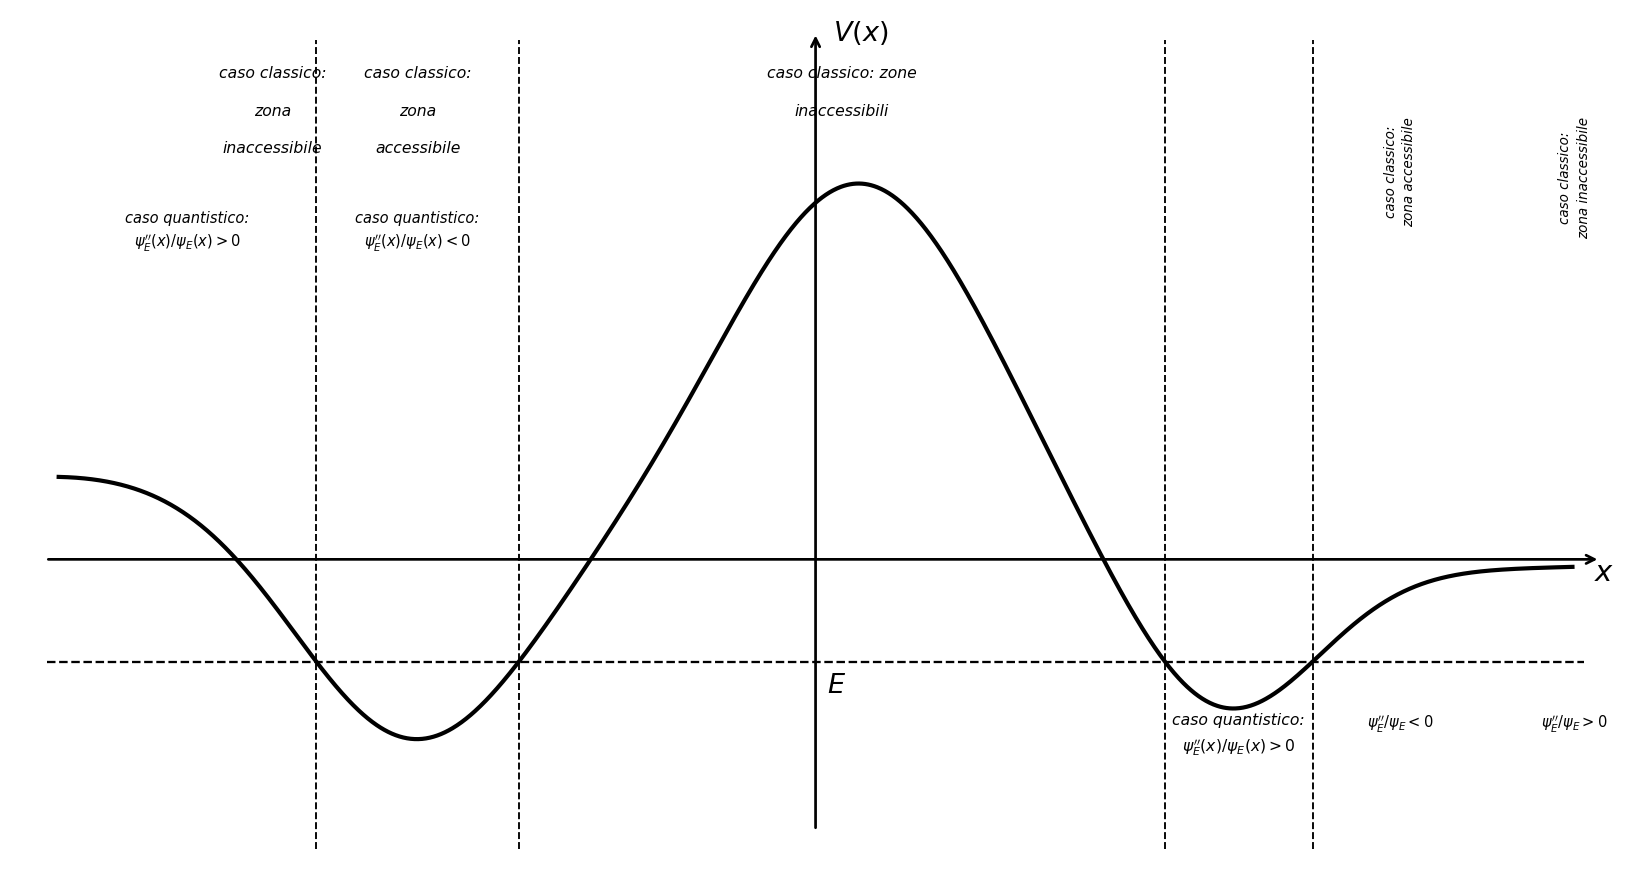
\includegraphics[width = 15cm]{images/p259.png}

L'interpretazione fisica di questo dilemma esorbita dagli argomenti
di questo corso, e ne lasciamo un'analisi ad altri corsi. Il solo punto che
ci preme notare è la possibilità che lo spettro di un operatore sia --- magari
solo in parte --- costituito da un continuo di valori (nell'esempio qui discusso,
tutti i valori positivi) anziché da una serie di valori discreti. Come già accennato precedentemente è questa possibilità che rende una trattazione rigorosa dal punto di vista matematico alquanto più difficile, specialmente per
quanto attiene alle proprietà di completezza delle autofunzioni di un operatore hermitiano.

È infine interessante osservare che lo spettro continuo risulta associato a problemi in cui, nel caso classico, un intervallo di estensione infi-

% --- pag. 260 ---

nita è accessibile al moto, laddove lo spettro discreto risulta associato a problemi per cui, nel caso classico, il moto è limitato ad un
intervallo finito (si noti che questo è sempre il caso, per ogni valore
dell'energia totale, se il potenziale diverge asintoticamente secondo
la (2); se il comportamento asintotico del potenziale è invece caratterizzato dalla (12), se cioè il potenziale si annulla asintoticamente, questo accade per energie totali negative). Questa associazione di spettro discreto ad
intervallo finito, e di spettro continuo ad intervallo infinito, caratterizzerà, come vedremo, anche la trattazione del capitolo seguente, dedicato a
serie ed integrali di Fourier.

\begin{esercizi}
\item Determinare tutti i livelli energetici negativi di una particella
unidimensionale di massa $m$ nel potenziale $V(x) = V_0\,[\cosh(x/a)]^{-2}$,
con $V_0 < 0$.\\
(Suggerimento: cercare autofunzioni della forma
\[
\psi(x) = \left[\cosh(x/a)\right]^{-\nu} \varphi(y) \,, \quad y = \sinh(x/a) \,,
\]
con $\nu$ opportuna costante, e sviluppare la $\varphi(y)$ in serie di potenze,
ponendo cioè
\[
\varphi(y) = \sum_{n=0}^{\infty} c_n\, y^n \quad ).
\]

\item Verificare le proprietà descritte nel paragrafo successivo alla equazione (19) per il caso dell'oscillatore armonico, usando le esplicite
espressioni dei polinomi di Hermite (vedi per esempio le (5-53)).
\end{esercizi}

\section{Principio di Ritz}

Nello studio degli spazi vettoriali finito-dimensionali avevamo dedotto,
dalla proprietà minimax degli autovalori, la validità del cosiddetto ``principio
di Ritz'' (in realtà, un teorema; vedi la sezione 3.4). Questo risultato resta
valido anche per gli operatori hermitiani agenti in spazi funzionali, sebbene
occorra tener presente che in questo caso gli operatori ammettono generalmente un numero infinito di autovalori.

Sia $A$ un operatore lineare hermitiano agente in uno spazio funzionale;
siano $a_n$ i suoi autovalori, ordinati in ordine crescente, cioè in modo che
\begin{equation}
a_{n+1} \geq a_n \,; \tag{1}
\end{equation}

% --- pag. 261 ---

siano $|a_n\rangle$ i corrispondenti autokets normalizzati, che per ipotesi
costituiscano un insieme non solo ortonormale ma anche completo:
\begin{equation}
(a_n \mid a_m) = \delta_{nm} \,, \tag{2}
\end{equation}
\begin{equation}
\sum_n |a_n)(a_n| = \mathbf{I} \,. \tag{3}
\end{equation}

Siano gli $|u_\ell\rangle$, $\ell = 1, 2, \ldots, p$, $p$ kets ortonormali,
cioè tali che
\begin{equation}
(u_\ell \mid u_m) = \delta_{\ell m} \,. \tag{4}
\end{equation}

Si definisca ora la matrice a $p$ righe e $p$ colonne
\begin{equation}
\tilde{A}_{\ell m} = (u_\ell \mid A \mid u_m) \,; \tag{5}
\end{equation}
questa matrice è hermitiana, come conseguenza della assunta hermiticitàdell'operatore $A$.

\textit{Dimostrazione:}
\begin{align*}
\tilde{A}^*_{m\ell} &= (u_m \mid A \mid u_\ell)^* \\
&= (u_\ell \mid A^+ \mid u_m) \quad \text{(per la (3-16))} \\
&= (u_\ell \mid A \mid u_m) \quad \text{(perché $A^+ = A$)} \\
&= \tilde{A}_{\ell m}
\end{align*}

Dunque la matrice $\tilde{A}$ di elementi $\tilde{A}_{\ell m}$ avrà $p$ autovalori reali
$\tilde{a}_n$, $n = 1, 2, \ldots, p$, che ordiniamo in ordine crescente, cioè
in modo che
\begin{equation}
\tilde{a}_{n+1} \geq \tilde{a}_n \,. \tag{6}
\end{equation}

Ebbene il teorema di Ritz afferma che
\begin{equation}
\tilde{a}_\ell \geq a_\ell \,, \quad \ell = 1, 2, \ldots, p \,; \tag{7}
\end{equation}

% --- pag. 262 ---

cioè i $p$ autovalori della matrice hermitiana a $p$ righe e $p$ colonne $\tilde{A}$,
eq.\ (5), costituiscono un limite superiore per i primi $p$ autovalori dell'operatore hermitiano $A$.

Si noti che il risultato testé enunciato è valido qualunque siano
i $p$ kets $|u_n\rangle$, purché soddisfino le condizioni di ortonormalità (4).
Inoltre se si ripete il calcolo con un più ampio insieme di kets,
costituito da $p' > p$ kets ed includente tutti i $p$ kets $|u_n\rangle$, i $p'$ autovalori così ottenuti non solo maggiorano i primi $p'$ autovalori di $A$, ma,
per i primi $p$ autovalori, forniscono una maggiorazione certamente non
meno stringente della precedente; cioè, se indichiamo con $\tilde{\tilde{a}}_\ell$ i $p'$
autovalori ottenuti col nuovo calcolo, vale per i primi $p$ di questi la
proprietà
\begin{equation}
\tilde{a}_n \geq \tilde{\tilde{a}}_n \geq a_n \,, \quad n = 1, 2, \ldots, p \,. \tag{8}
\end{equation}

In effetti si può dire (in modo non proprio rigoroso) che al crescere del numero $p$ dei kets ortonormali $|u_n\rangle$, gli autovalori $\tilde{a}_n$ dell'operatore hermitiano $A$.

Nella formulazione fornita sino a questo punto si è implicitamente
sottinteso che lo spettro degli autovalori $a_n$ di $A$ abbia un valore minimo $a_1$ (se ciò non fosse, non sarebbe possibile numerare gli autovalori
a partire dal più piccolo, e la enunciazione dei risultati dati finora cadrebbe).
Se lo spettro degli autovalori di $A$ ha un valore massimo, la formulazione
data finora può ripetersi in modo speculare, ordinando gli autovalori a partire dal più grande; in tal caso l'autovalore $\tilde{a}_n$ fornisce un limite inferiore (ovverosia una approssimazione per difetto) all'autovalore $a_n$.

Non diamo una dimostrazione del risultato enunciato, limitandoci a
dimostrare il caso più semplice in cui si ha un solo ket $|u\rangle$ ($p = 1$); è
del resto questo il teorema che viene generalmente denotato come ``principio di Ritz'', e viene usato più di frequente. Tale risultato si può enunciare nel modo seguente:
\begin{equation}
a_{\min} \leq (u \mid A \mid u) / (u \mid u) \leq a_{\max} \,, \tag{9}
\end{equation}
dove con $a_{\min}$ abbiamo indicato il più piccolo degli autovalori dello
operatore hermitiano $A$ (se esiste), ed $|u\rangle$ è un arbitrario ket (non necessariamente normalizzato; il fattore di normalizzazione
è stato introdotto esplicitamente nella (9)).

% --- pag. 263 ---

La dimostrazione si fonda sulla ipotizzata completezza dello
insieme degli autostati di $A$, che implica la possibilità di scrivere
il generico stato $|u\rangle$ come sovrapposizione di tali stati:
\begin{equation}
|u\rangle = \sum_{n=1}^{\infty} c_n\, |a_n\rangle \,. \tag{10}
\end{equation}

Questa formula implica, per la ortonormalità degli $|a_n\rangle$ (che segue
dalla assunta hermiticitàdell'operatore $A$)
\begin{equation}
(u \mid u) = \sum_{n=1}^{\infty} |c_n|^2 \tag{11}
\end{equation}
e
\begin{equation}
(u \mid A \mid u) = \sum_{n=1}^{\infty} |c_n|^2\, a_n \,. \tag{12}
\end{equation}

Dalla (12) segue
\begin{align}
(u \mid A \mid u) &\geq a_{\min} \sum_{n=1}^{\infty} |c_n|^2 \,, \tag{13a} \\
(u \mid A \mid u) &\leq a_{\max} \sum_{n=1}^{\infty} |c_n|^2 \,, \tag{13b}
\end{align}
per la definizione stessa di $a_{\min}$ e $a_{\max}$; e dalle (13) e (11) segue
la (9), c.v.d.

In questa discussione si è implicitamente assunto che lo spettro di
$A$ fosse discreto; ma è chiaro che il risultato testé enunciato è valido
generalmente, anche nel caso di spettro continuo.

La quantità $(u \mid A \mid u) / (u \mid u)$, qualunque sia $|u\rangle$,
fornisce dunque un limite superiore per $a_{\min}$ (ed un limite inferiore
per $a_{\max}$). Inoltre, se lo stato $|u\rangle$ non si discosta troppo dallo
stato $|a_{\min}\rangle$, allora la quantità $(u \mid A \mid u) / (u \mid u)$ fornisce
una buona approssimazione (per eccesso) di $a_{\min}$. In effetti è
facile dimostrare che, se lo stato $|u\rangle$ differisce dallo stato $|a_{\min}\rangle$
per quantità piccole di ordine $\varepsilon$, la quantità $(u \mid A \mid u) / (u \mid u)$
differisce da $a_{\min}$ per una quantità piccola di ordine $\varepsilon^2$.

Infatti scriviamo la (10) nella forma
\begin{equation}
|u\rangle = c_1\, |a_1\rangle + \eta\, |\ \rangle \,, \tag{14}
\end{equation}

% --- pag. 264 ---

con
\begin{equation}
\eta\, |\,\rangle = \sum_{n=2}^{\infty} c_n\, |a_n\rangle \tag{15}
\end{equation}
\begin{equation}
(\,|\,) = 1 \,, \tag{16}
\end{equation}
che implica
\begin{equation}
|\eta|^2 = \sum_{n=2}^{\infty} |c_n|^2 \,. \tag{17}
\end{equation}

Affinché lo stato $|u\rangle$ non differisca troppo dallo stato $|a_1\rangle$ (a meno
della normalizzazione), la quantità
\begin{equation}
\varepsilon = |\eta| / |c_1| \tag{18}
\end{equation}
dovrà essere piccola; ed il valore di questa quantità è una misura di
quanto lo stato $|u\rangle$ differisce (a parte la normalizzazione) da $|a_1\rangle$.

Ma d'altra parte si dimostra facilmente che
\begin{equation}
(u \mid A \mid u) / (u \mid u) = a_1 + \left[\varepsilon^2/(1+\varepsilon^2)\right]\left[(|A|) - a_1\right], \tag{19}
\end{equation}
che mostra appunto come $(u \mid A \mid u)/(u \mid u)$ differisce da $a_1$ solo per
termini di ordine $\varepsilon^2$.

\textit{Dimostrazione:} dalla (15) segue che lo stato $|\,\rangle$ è ortogonale
allo stato $|a_1\rangle$. Pertanto, per le (14) e (16),
\[
(u \mid u) = |c_1|^2 + |\eta|^2 \,,
\]
nonché
\[
(u \mid A \mid u) = a_1\, |c_1|^2 + |\eta|^2\, (|A|) \,.
\]
Pertanto
\[
(u \mid A \mid u)/(u \mid u) = \left[a_1\, |c_1|^2 + |\eta|^2\, (|A|)\right] / \left[|c_1|^2 + |\eta|^2\right] \,,
\]
e da questa segue, con elementari passaggi, la (19), c.v.d.

% --- pag. 265 ---

Si noti per inciso che la (19) costituisce una ulteriore dimostrazione del teorema di Ritz, se si osserva che le definizioni (15)
e (16) implicano
\begin{equation}
(|A|) \geq a_2 \geq a_1 \tag{20}
\end{equation}
(si ricordi che stiamo sempre assumendo che gli autovalori siano
ordinati in ordine crescente, nella ipotesi che esista un autovalore
minimo, $a_{\min}$, cui assegnare il numero d'ordine $n = 1$).

\textit{Dimostrazione della (20):}
\begin{align*}
|\eta|^2\, (|A|) &= \sum_{n=2}^{\infty} |c_n|^2\, a_n \quad \text{(per la (15))} \\
&\geq a_2 \sum_{n=2}^{\infty} |c_n|^2 \\
&= |\eta|^2\, a_2 \quad \text{(per la (17))}
\end{align*}

Il risultato testé dimostrato implica dunque che, per una scelta
giudiziosa della ``funzione di prova'' $|u\rangle$, la quantità $(u \mid A \mid u)/(u \mid u)$
fornisce uno stringente limite superiore per $a_1$, cioè una buona approssimazione per eccesso. La scelta di $|u\rangle$ costituirà un compromesso
fra la esigenza che $|u\rangle$ sia semplice, in modo che risulti agevole
il calcolo di $(u \mid A \mid u)$, e l'esigenza che $|u\rangle$ sia flessibile,
per poter meglio approssimare lo stato incognito $|a_1\rangle$ (questa seconda
esigenza è generalmente realizzata facendo dipendere $|u\rangle$ da dei parametri, i cui valori possono essere poi fissati minimizzando la quantità
$(u \mid A \mid u) / (u \mid u)$; il vantaggio del principio di Ritz rispetto ad
altri metodi approssimati è per l'appunto dovuto all'esistenza di un tale
criterio, che permette di scegliere, entro un insieme di funzioni di prova,
la migliore).

In questa ultima discussione si è fatto riferimento al caso in cui
lo spettro dell'operatore hermitiano $A$ contenga un autovalore minimo,
ed in cui ci si ponga come obbiettivo quello di calcolare, eventualmente
in modo approssimato, tale autovalore minimo. È ovvio come questa
analisi andrebbe modificata nel caso in cui esista, e si voglia determi-

% --- pag. 266 ---

nare, l'autovalore massimo di $A$.

La più consueta utilizzazione del principio di Ritz si effettua, nell'ambito della teoria quantica, per la determinazione dello
autovalore più basso dell'operatore hamiltoniano rappresentante l'energia totale di un sistema --- autovalore cui corrisponde lo ``stato fondamentale'' del sistema stesso.

Terminiamo questa sezione sottolineando che la dimostrazione
del teorema di Ritz utilizza l'ipotesi che l'operatore hermitiano $A$ abbia
un \underline{sistema completo} di autostati; occorre dunque che sia opportunamente definito lo spazio funzionale in cui tale operatore agisce.

\begin{esercizi}
\item Si consideri il sistema quantico costituito da una particella di
massa $m$, vincolata a muoversi lungo l'asse delle $x$, ed ivi
soggetta al potenziale
\[
V(x) = V_0\, e^{-\mu|x|} \,, \quad \mu > 0 \,,
\]
(vedi la sezione 9). Si determini, usando il metodo di Ritz, un valore
$V_M$ tale che, per $V_0 < V_M$, il sistema ammette certamente
almeno due stati ad energia negativa, che saranno dunque descritti
da funzioni d'onda normalizzabili.\\
(Suggerimento: si usino le due funzioni di prova
\[
u_1(x) = c_1\, e^{-\mu_1 |x|} \,, \quad \mu_1 > 0 \,,
\]
e
\[
u_2(x) = c_2\, x\, e^{-\mu_2 |x|} \,, \quad \mu_2 > 0 \quad ).
\]

\item[*] Si confronti il risultato con quello che si ottiene risolvendo
esattamente il problema (per far ciò, sfruttare il fatto che, per
$x \geq 0$, passando alla variabile $y = \exp(-\frac{1}{2}\mu x)$, l'equazione di
Schroedinger può ricondursi alla equazione per le funzioni di Bessel
(ed analogamente per $x \leq 0$); ed utilizzare le proprietà di tali
funzioni, ivi compresi i loro valori numerici, che potranno essere
desunti dalle apposite tabelle (cfr., per esempio, E.\ Jahnke and
F.\ Emde, \emph{Tables of functions}, Dover, New York, 1945, ovvero
\emph{Handbook of Mathematical Functions} (M.\ Abramowitz e I.A.\ Stegun,
editors), National Bureau of Standards, Washington, 1964)).
\end{esercizi}

\section*{4.S \quad Soluzioni degli esercizi del capitolo 4.}

\begin{description}
\item[1-1] Si salva nei casi (v) e (vii).

\item[1-2]
\begin{itemize}
  \item[(i)] $c > -3/2$\,;
  \item[(ii)] $c > -3/2$\,;
  \item[(iii)] $-\tfrac{1}{2} < c < -\tfrac{1}{c}$\,; % [DUBBIO: la condizione iii è parzialmente illeggibile]
  \item[(iv)] $c > 0$\,;
  \item[(v)] $c < \tfrac{1}{2}$ oppure $c > 1$\,;
  \item[(vi)] $c = 2\pi m$, $m$ intero\,;
  \item[(vii)] $c = -\pi$\,;
  \item[(viii)] $c$ reale arbitrario.
\end{itemize}

\item[1-3] $|f| = \sqrt{\pi/2}$.

\item[1-4] $|f - g| = \sqrt{3\pi/2}$.

\item[2-1] Nessuno.

\item[2-2] $F(t)$ deve essere una funzione reale, cioè $F(t) = F(t)^*$ per $t$ reale.

\item[2-3] Per $n$ dispari, $c_n$ deve essere immaginario puro, e per $n$ pari reale:
\[
  c_n^* = (-)^n\, c_n\,.
\]
La dimostrazione si effettua integrando ripetutamente per parti ed utilizzando il fatto che i contributi dagli estremi di integrazione sono sempre nulli, poiché le funzioni dello spazio funzionale, per essere di modulo quadrato sommabile con tutte le loro derivate, devono annullarsi asintoticamente (per $x \to \pm\infty$) con tutte le loro derivate.

\item[2-4] $A$ e $B$ devono commutare.

\item[2-5] No, anzi, è antihermitiano:
\[
  A = A^\dagger,\quad B = B^\dagger,\quad C = [A,B] \quad\text{implica}\quad C^\dagger = -C\,.
\]

\item[2-6] $\left[\dfrac{d}{dx},\, x\right] = I$.

\item[2-7] $\left[\dfrac{d}{dx},\, F(x)\right] = F'(x)$.

\item[2-8]
\[
  H = \tfrac{1}{2}\!\left(-\frac{d^2}{dx^2} + x^2 - 1\right),
\]
\[
  [A, A^\dagger] = I,\quad [H, A] = -A,\quad [H, A^\dagger] = A^\dagger.
\]

\item[2-9]
\[
  \exp\!\left(\alpha\frac{d}{dx}\right) f(x)
  = \sum_{n=0}^{\infty} \frac{\alpha^n}{n!}\, f^{(n)}(x)
  = f(x + \alpha)
\]
(per il teorema di Taylor).

\item[2-10] No. Per esempio la funzione $f = (1+x^2)^{-1}\sin(x^2)$ appartiene a tale spazio, ma $df/dx$ non appartiene (la sua derivata non è quadrato sommabile).

\item[2-11]
\[
  e^{\frac{1}{2}\alpha x^2}\,\frac{d}{dx}\!\left[e^{-\frac{1}{2}\alpha x^2} f(x)\right]
  = -\alpha x\, f(x) + \frac{d\,f(x)}{dx}\,.
\]

\item[4-1] Solo i casi i) e iv) sono autofunzioni; i corrispondenti autovalori sono $3/2$ e $5/2$, e i coefficienti di normalizzazione $c$ (tali cioè che $c\,\varphi(x)$ sia normalizzata) sono rispettivamente $2^{1/2}\pi^{-1/4}$ e $2^{-3/2}\pi^{-1/4}$.

\item[4-2] No. Infatti $H\,|h\rangle = h\,|h\rangle$ ovvero $A^\dagger A\,|h\rangle = h\,|h\rangle$ implica $(h\,|\,A^\dagger A\,|\,h) = h\,(h|h)$ donde $h = |A|h\rangle|^2 \geq 0$.

\item[5-1]
\[
  x_n = \sum_{m=0}^{p-1} x_n^{(m)},
\]
\[
  x_n^{(m)} = x_m \prod_{\ell=1}^{\bar{\ell}} c_{m+\ell p},
\]
$x_n^{(m)}$ se $\bar{\ell} = (n-m)/p$ è un intero positivo, $x_n^{(m)} = 0$ se $\bar{\ell}$ non è un intero positivo. Le quantità $x_m$, $m=0,1,\ldots,p-1$, sono arbitrarie, e la assegnazione dei loro valori costituisce le ulteriori condizioni da assegnare, in aggiunta alle relazioni ricorrenti, affinché le incognite $x_n$, per $n \geq p$, risultino tutte determinate.

\item[5-2]
\[
  H_n(x) = n!\sum_{m=0}^{[n/2]} \frac{(-)^m\,(2x)^{n-2m}}{m!\,(n-2m)!}\,,
\]
$[n/2] = n/2$ se $n$ è pari, $[n/2]=(n-1)/2$ se $n$ è dispari.

\item[5-4] L'equazione differenziale soddisfatta dai polinomi di Hermite si ottiene per semplice sostituzione della (56) nella (3), con $h$ dato dalla (28) (in realtà questa equazione è già stata scritta, vedi la (12)). Le due relazioni ricorrenti seguono dalle (56), (46) e (31), e la terza segue dalle prime due.

\item[5-6]
\begin{align*}
  \sum_{n=0}^{\infty} \frac{t^n}{n!}\, H_n(x)
  &= e^{x^2} \sum_{n=0}^{\infty} \frac{(-tD)^n}{n!}\, e^{-x^2}
    \quad\text{(per la (52b))}\\
  &= e^{x^2}\, e^{-tD}\, e^{-x^2}\\
  &= e^{x^2}\, \exp\!\left[-(x-t)^2\right]
    \quad\text{(vedi l'esercizio 2-9)}\\
  &= e^{2xt - t^2}\,.
\end{align*}
In questi passaggi, per comodità di scrittura, si è indicato con $D$ l'operatore $d/dx$.

\item[5-7]
\begin{align*}
  e^{-t^2+2xt} &= \sum_{n=0}^{\infty} \frac{H_n(x)\,t^n}{n!}\,,\\
  e^{2xt} &= e^{t^2}\sum_{\ell=0}^{\infty} \frac{H_\ell(x)\,t^\ell}{\ell!}\,,\\
  \sum_{n=0}^{\infty} \frac{(2xt)^n}{n!}
  &= \sum_{m=0}^{\infty} \frac{t^{2m}}{m!} \sum_{\ell=0}^{\infty} \frac{H_\ell(x)\,t^\ell}{\ell!}\,,\\
  \sum_{n=0}^{\infty} \frac{(2x)^n}{n!}\,t^n
  &= \sum_{n=0}^{\infty} t^n \sum_{m=0}^{[n/2]} \frac{H_{n-2m}(x)}{m!\,(n-2m)!}\,.
\end{align*}
L'ultimo passaggio è stato eseguito ponendo $n = \ell + 2m$. Uguagliando i coefficienti di $t^n$ a primo e secondo membro, si ottiene per l'appunto la formula che si voleva dimostrare.

\item[5-8] Se $n-m$ è dispari, l'integrando è dispari e quindi l'integrale è nullo. Se $n>m$, nello sviluppo di $x^n$ in polinomi di Hermite (vedi esercizio precedente) il polinomio $H_m(x)$ non è contenuto, e quindi di l'integrale si annulla per la ortogonalità delle $\psi_n(x) = c_n H_n(x) e^{-\frac{1}{2}x^2}$ con indici $n,m$ diversi. Se $n-m = 2K$ con $K$ intero non negativo, sostituendo ad $x^n$ il suo sviluppo (vedi esercizio precedente) si ottiene
\begin{align*}
  \int_{-\infty}^{+\infty} dx\; e^{-x^2}\, x^n\, H_m(x)
  &= \sum_{\ell=0}^{[n/4]} % [DUBBIO: limite superiore della somma]
    \frac{n!}{2^n\,\ell!\,(n-2\ell)!}
    \cdot \int_{-\infty}^{+\infty} dx\; e^{-x^2}\, H_{n-2\ell}(x)\, H_m(x)\\
  &= \frac{n!\,m!\,2^m\sqrt{\pi}}{2^n\left[(\tfrac{n}{2}-m)!\right] m!}\,,
\end{align*}
che corrisponde per l'appunto alla formula che si voleva dimostrare.

\item[5-9]
\begin{align*}
  \exp\!\left[-(t+y)^2 + 2x(t+y)\right]
  &= \sum_{\ell=0}^{\infty} \frac{H_\ell(x)\,(t+y)^\ell}{\ell!}\\
  &= \sum_{\ell=0}^{\infty} \frac{H_\ell(x)}{\ell!} \sum_{m=0}^{\ell} t^{\ell-m} y^m \binom{\ell}{m}
    \quad\text{(usando la formula della potenza di un binomio)}\\
  &= \sum_{\ell=0}^{\infty} H_\ell(x) \sum_{m=0}^{\ell} \frac{t^{\ell-m}\cdot y^m}{m!\,(\ell-m)!}\\
  &= \sum_{n=0}^{\infty} \frac{t^n}{n!} \sum_{m=0}^{\infty} \frac{y^m\, H_{m+n}(x)}{m!}
    \,,\quad (\ell-m=n)
\end{align*}
\begin{align*}
  \exp\!\left[-(t+y)^2 + 2x(t+y)\right]
  &= \exp\!\left[-y^2+2xy\right] \exp\!\left[-t^2+2t(x-y)\right]\\
  &= \exp\!\left[-y^2+2xy\right] \sum_{n=0}^{\infty} \frac{t^n}{n!}\, H_n(x-y)\,.
\end{align*}
Identificando i coefficienti di $t^n$ nelle due espressioni date si ottiene il risultato richiesto.

\item[5-10] Questi risultati seguono immediatamente dalle formule esplicite dei polinomi di Hermite, vedi l'esercizio 5-2.

\item[5-11]
\[
  \exp\!\left[-t^2 + 2(x+y)\,t\right] = \sum_{n=0}^{\infty} \frac{t^n}{n!}\, H_n(x+y)\,,
\]
\begin{align*}
  \exp\!\left[-\tfrac{1}{2}t^2+2x\,t\right]
  \exp\!\left[-\tfrac{1}{2}t^2+2y\,t\right]
  &= \exp\!\left[-\!\left(\tfrac{t}{\sqrt{2}}\right)^2 + 2\sqrt{2}\,x\,\tfrac{t}{\sqrt{2}}\right]
     \exp\!\left[-\!\left(\tfrac{t}{\sqrt{2}}\right)^2 + 2\sqrt{2}\,y\,\tfrac{t}{\sqrt{2}}\right]\\
  &= \sum_{m=0}^{\infty} \left(\frac{t}{\sqrt{2}}\right)^m \frac{H_m(\sqrt{2}\,x)}{m!}
     \sum_{\ell=0}^{\infty} \left(\frac{t}{\sqrt{2}}\right)^\ell \frac{H_\ell(\sqrt{2}\,y)}{\ell!}\\
  &= \sum_{n=0}^{\infty} \frac{t^n}{2^{n/2}} \sum_{m=0}^{n}
     \frac{H_m(\sqrt{2}\,x)\,H_{n-m}(\sqrt{2}\,y)}{m!\,(n-m)!}\,,
     \quad(m+\ell=n).
\end{align*}
Eguagliando i coefficienti delle stesse potenze di $t$ la formula data risulta dimostrata.

\item[5-12] Si dimostra in modo analogo a quello usato nel caso precedente, partendo dalle identità
\[
  \exp\!\left[-t^2 + 2t\sum_{s=1}^{p} \alpha_s x_s\right]
  = \prod_{s=1}^{p} \exp\!\left[-\frac{\alpha_s^2}{\alpha^2}\,t^2 + 2t\,\alpha_s x_s\right]
\]
con
\[
  \alpha^2 = \sum_{s=1}^{p} \alpha_s^2\,.
\]

\item[5-13] La prima formula è semplicemente un caso particolare della formula dell'esercizio precedente ($p=2$, $\alpha_1=\cos\theta$, $\alpha_2=\sin\theta$, $x_1=x$, $x_2=y$). La seconda formula si ricava facilmente dalla prima ponendo in essa $\cos\theta = \lambda$, $y=0$, e usando i valori di $H_\ell(0)$ (vedi esercizio 5-10).

\item[6-1] La serie converge uniformemente (al valore $(1-x)^{-1}$) per $-\frac{1}{2}\leq x \leq \frac{1}{2}$; converge (allo stesso valore), ma non uniformemente, nell'intervallo $-1<x<1$; non converge nel punto $x=+1$ (e dunque nemmeno nell'intervallo $-1\leq x\leq 1$).

\item[6-3]
\begin{align*}
  x_{nm} &= (n\,|\,x\,|\,m) = \frac{1}{\sqrt{2}}\,(n\,|\,A+A^\dagger\,|\,m)\\
  &= \frac{1}{\sqrt{2}}\left(\sqrt{m}\;\delta_{n,m-1} + \sqrt{n}\;\delta_{m,n-1}\right),\\[6pt]
  D_{nm} &= \left(n\,\left|\,\frac{d}{dx}\,\right|\,m\right) = \frac{1}{\sqrt{2}}\,(n\,|\,A-A^\dagger\,|\,m)\\
  &= \frac{1}{\sqrt{2}}\left(\sqrt{m}\;\delta_{n,m-1} - \sqrt{n}\;\delta_{m,n-1}\right),\\[6pt]
  (x^2)_{nm} &= (n\,|\,x^2\,|\,m) = x_{n\ell}\,x_{\ell m}\\
  &= \frac{1}{2}\Bigl(\sqrt{(n+1)m}\;\delta_{n,m-2} + \sqrt{(m+1)n}\;\delta_{m,n-2}
    + \bigl[\sqrt{nm}+\sqrt{(n+1)(m+1)}\bigr]\delta_{n,m}\Bigr),\\[6pt]
  (D^2)_{nm} &= \left(n\,\left|\,\frac{d^2}{dx^2}\,\right|\,m\right) = D_{n\ell}\,D_{\ell m}\\
  &= \frac{1}{2}\Bigl(\sqrt{(n+1)m}\;\delta_{n,m-2} + \sqrt{(m+1)n}\;\delta_{m,n-2}
    - \bigl[\sqrt{nm}+\sqrt{(n+1)(m+1)}\bigr]\delta_{n,m}\Bigr).
\end{align*}

\item[6-4]
\begin{align*}
  \operatorname{tr}\!\left[\exp\!\left\{-\frac{\beta}{2}\!\left(-\frac{d^2}{dx^2}+x^2\right)\right\}\right]
  &= \sum_{n=0}^{\infty} \exp\!\left\{-\beta\!\left(n+\tfrac{1}{2}\right)\right\}\\
  &= e^{-\beta/2}\left[1-e^{-\beta}\right]^{-1}
    \quad\text{(serie geometrica)}\\
  &= \left[2\sinh(\beta/2)\right]^{-1}.
\end{align*}

\item[6-5]
\begin{align*}
  \det\!\left[\alpha\Big/\!\left(\frac{d^2}{dx^2}-x^2\right)^2\right]
  &= \prod_{n=0}^{\infty} \exp\!\left[\alpha/(2n+1)^2\right]\\
  &= \exp\!\left[\alpha\sum_{n=0}^{\infty}(2n+1)^{-2}\right]\\
  &= \exp\!\left[\alpha\pi^2/8\right].
\end{align*}

\item[7-1] Tutti, salvo in qualche caso eccezionale la non degenerazione degli autovalori (vedi l'esercizio 7-3).

\item[7-2]
\[
  \lambda_n = n^2\pi^2/(\beta-\alpha)^2,\quad n=1,2,3,\ldots,
\]
\[
  y_n(x) = \left[(\beta-\alpha)/2\right]^{-\frac{1}{2}}
  \sin\!\left[n\pi\,(x-\alpha)/(\beta-\alpha)\right].
\]

\item[7-3]
\begin{itemize}
  \item[i)]
  \[
    \lambda_n = n^2\pi^2/(\beta-\alpha)^2,\quad n=0,1,2,\ldots,
  \]
  \[
    y_n(x) = \left[(1+\delta_{n,0})\,(\beta-\alpha)/2\right]^{-\frac{1}{2}}
    \cos\!\left[n\pi\,(x-\alpha)/(\beta-\alpha)\right];
  \]
  \item[ii)] Gli autovalori $\lambda_n$ sono dati dalla soluzione dell'equazione trascendente
  $\lambda_n = \nu_n^2$, essendo $\nu_n$ soluzione di
  \[
    \tan\!\left[\nu(\beta-\alpha)\right] = \nu(k_1-k_2)/(\nu^2+k_1 k_2),
  \]
  (per discutere questa equazione, fare il grafico del primo e secondo membro come funzioni di $\nu$ per $\nu>0$; i valori di $\nu_n$ della equazione trascendente, sono le radici in corrispondenza ai quali i grafici si intersecano. Si considerino separatamente il caso in cui i segni di $k_1$ e $k_2$ sono concordi o discordi, e la differenza $k_1-k_2$ è positiva o negativa). Le corrispondenti autofunzioni sono
  \[
    y_n(x) = C_n \cos(\nu_n x) + S_n \sin(\nu_n x),
  \]
  con $C_n$ ed $S_n$ fissati dalla equazione
  \[
    C_n\left[\nu\sin(\nu\alpha)+k_1\cos(\nu\alpha)\right]
    = S_n\left[\nu\cos(\nu\alpha)-k_1\sin(\nu\alpha)\right],
  \]
  e eventualmente dalla condizione che $y_n(x)$ sia normalizzata. Se $k_1=k_2$, $\nu_n = n\pi/(\beta-\alpha)$, $n=1,2,3,\ldots$;
  \item[iii)]
  \[
    \lambda_n = 4n^2\pi^2/(\beta-\alpha)^2,\quad n=0,1,2,3,\ldots
  \]
\end{itemize}

In questo caso eccezionale ogni autovalore è degenere (salvo il primo!) corrispondendo ad esso le due autofunzioni (normalizzate) indipendenti
\[
  y_n^{(1)}(x) = \left[2/(\beta-\alpha)\right]^{\frac{1}{2}}
  \sin\!\left[2\pi n\,x/(\beta-\alpha)\right],\quad n=1,2,3,\ldots,
\]
\[
  y_n^{(2)}(x) = \left[2/(\beta-\alpha)\right]^{\frac{1}{2}}
  \cos\!\left[2\pi n\,x/(\beta-\alpha)\right],\quad n=1,2,3,\ldots
\]
E in effetti si può verificare che in corrispondenza agli autovalori $\lambda_n = 4n^2\pi^2/(\beta-\alpha)^2$ con $n=1,2,3,\ldots$, qualunque soluzione della equazione differenziale soddisfa le condizioni al contorno $y(\alpha)=y(\beta)$, $y'(\alpha)=y'(\beta)$, semplicemente perché risulta essere una funzione periodica con periodo $\beta-\alpha$. Per l'autovalore (non degenere) $\lambda_0=0$ si ha invece la sola autofunzione costante
\[
  y_0(x) = (\beta-\alpha)^{-\frac{1}{2}}.
\]
  \begin{itemize}
    \item[iv)] Poiché in questo caso $p(x)=1$, questo caso coincide col precedente.
  \end{itemize}

\item[7-4]
\begin{align*}
  P_0(x) &= 1,\\
  P_1(x) &= x,\\
  P_2(x) &= \tfrac{1}{2}(3x^2-1),\\
  P_3(x) &= \tfrac{1}{2}(5x^3-3x),\\
  P_4(x) &= \tfrac{1}{8}(35x^4-30x^2+3).
\end{align*}

\item[7-5] Si usi la formula di Leibniz della potenza di un binomio, che implica
\[
  (x^2-1)^n = \sum_{\ell=0}^{n} \frac{(-)^{n-\ell}\,n!\,x^{2\ell}}{\ell!\,(n-\ell)!}\,;
\]
si inserisca questa equazione nella (25), si differenzi termine a termine, e si cambi infine l'indice nella somma, ponendo $2\ell-n = n-2m$.

\item[7-6] Basta verificare che i coefficienti $c_{n,m}$ desumibili dalla (23) scrivendola nella forma
\[
  P_n(x) = \sum_{m=0}^{n} c_{n,m}\, x^m\,,
\]
soddisfano alle regole ricorrenti (18), cioè
\[
  c_{n,m+2} = c_{n,m}\,\frac{[m(m+1)-n(n+1)]}{(m+2)(m+1)}\,,\quad m=0,1,2,\ldots,
\]
con condizioni iniziali
\[
  c_{n,1} = 0 \quad\text{se } n \text{ è pari},\qquad
  c_{n,0} = 0 \quad\text{se } n \text{ è dispari}.
\]
I coefficienti $c_{n,0}$ (se $n$ è pari) e $c_{n,1}$ (se $n$ è dispari) sono fissati a posteriori dalla condizione $P_n(1)=1$. Il modo più diretto di determinarli è usando la dimostrata equivalenza dei secondi membri delle (23) e (25) (vedi esercizio precedente), e il fatto che, per $x=1$, il secondo membro della (25) vale certamente 1 (l'unico termine che sopravvive per $x=1$ è quello in cui la derivata ha per $n$ volte abbassato il grado del binomio).

\item[7-7] Sia $n\geq m$:
\begin{align*}
  \int_{-1}^{1} dx\; P_n(x)\,P_m(x)
  &= \left[(2^n n!)(2^m m!)\right]^{-1}
    \int_{-1}^{1} dx\;\frac{d^n}{dx^n}(x^2-1)^n\;\frac{d^m}{dx^m}(x^2-1)^m\\
  &= (-)^n\left[2^n n!\;2^m m!\right]^{-1}
    \int_{-1}^{1} dx\;(x^2-1)^n\;\frac{d^{n+m}}{dx^{n+m}}(x^2-1)^m.
\end{align*}
Il secondo passaggio è stato effettuato integrando $n$ volte per parti. Ma se $n>m$,
\[
  \frac{d^{n+m}}{dx^{n+m}}(x^2-1)^m = 0,
\]
mentre se $n=m$
\[
  \frac{d^{n+m}}{dx^{n+m}}(x^2-1)^m = \frac{d^{2n}}{dx^{2n}}(x^2-1)^n = (2n)!\,.
\]
Pertanto
\[
  \int_{-1}^{1} dx\; P_n(x)\,P_m(x)
  = \delta_{nm}\,(-)^n\,\bigl(2^n n!\bigr)^{-2}(2n)!\int_{-1}^{1} dx\;(x^2-1)^n\,.
\]
Ma come è noto
\begin{align*}
  \int_{-1}^{1} dx\;(x^2-1)^n
  &= 2(-)^n \int_{0}^{1} dx\;(1-x^2)^n\\
  &= 2(-)^n \int_{0}^{\pi/2} d\theta\;(\cos\theta)^{2n+1}
  = 2(-)^n\,(2n)!!\,/\,(2n+1)!!\,,
\end{align*}
sicché
\[
  \int_{-1}^{1} dx\; P_n(x)\,P_m(x)
  = \delta_{nm}\;2\,\bigl(2^n n!\bigr)^2 (2n)!\,(2n)!!\,/\,(2n+1)!!\,.
\]
Il risultato richiesto segue usando le ovvie formule
\[
  (2n)!! = 2^n\,n!\,,\qquad (2n+1)!!\,(2n)!! = (2n+1)!\,.
\]

\item[7-8] Si moltiplichi la (29) per $P_m(x)$, si integri da $-1$ ad $1$ e si usi la (22).

\item[7-12] Gli operatori $x$ e $x^2$ sono hermitiani; $D$ non è hermitiano (né antihermitiano), nello spazio funzionale in questione. La loro rappresentazione esplicita nella base data è fornita dalle matrici
\begin{align*}
  x_{nm} &= \left[(2n+1)(2m+1)\right]^{-\frac{1}{2}}
    \left[n\,\delta_{n,m+\frac{1}{2}} + m\,\delta_{m,n+1}\right], % [DUBBIO: indici delta illeggibili]
  \\[4pt]
  (x^2)_{nm} &= \left[(2n+1)(2m+1)\right]^{-\frac{1}{2}}
    \left\{\frac{n(n-1)}{2n-1}\,\delta_{n,m+2}
    + \frac{m(m-1)}{2n-1}\,\delta_{m,n+2} % [DUBBIO]
    + \left[\frac{n^2}{2n-1}+\frac{(n+1)^2}{2n+3}\right]\delta_{n,m}\right\},
  \\[4pt]
  D_{nm} &= \left[(2n+1)(2m+1)\right]^{1/2}\quad\text{se } m=n+1,n+3,n+5,\ldots,\\
  D_{nm} &= 0\quad\text{altrimenti}.
\end{align*}
La espressione di $x_{nm}$ è ricavata usando la (26); la espressione di $(x^2)_{nm}$ è ottenuta usando ripetutamente la (26), oppure usando $x^2_{nm} = x_{n\ell}\,x_{\ell m}$; l'espressione nella formula data nell'esercizio precedente. Oltre alle equazioni indicate, si è naturalmente anche usata la (22).

\item[7-13]
\begin{align*}
  V(r,\theta) &= q_1/r_1 + q_2/r_2\\
  &= q_1/\!\left[r^2+d^2+2rd\cos\theta\right]^{\frac{1}{2}}
   + q_2/\!\left[r^2+d^2-2rd\cos\theta\right]^{\frac{1}{2}}\\
  &= (q_1/d)\left[1+2(r/d)\cos\theta+(r/d)^2\right]^{-\frac{1}{2}}
   +(q_2/d)\left[1-2(r/d)\cos\theta+(r/d)^2\right]^{-\frac{1}{2}}\\
  &= (q_1/r)\left[1+2(d/r)\cos\theta+(d/r)^2\right]^{-\frac{1}{2}}
   +(q_2/r)\left[1-2(d/r)\cos\theta+(d/r)^2\right]^{-\frac{1}{2}}
\end{align*}
\[
  V(r,\theta) = d^{-1}\sum_{n=0}^{\infty}\bigl[q_2+(-)^n q_1\bigr](r/d)^n P_n(\cos\theta),\quad r<d,
\]
\[
  V(r,\theta) = r^{-1}\sum_{n=0}^{\infty}\bigl[q_2+(-)^n q_1\bigr](d/r)^n P_n(\cos\theta),\quad r>d.
\]
Per $q_1=-q$, $q_2=q$:
\[
  V(r,\theta) = 2(q/d)\sum_{m=0}^{\infty}(r/d)^{2m+1} P_{2m+1}(\cos\theta),\quad r<d,
\]
\[
  V(r,\theta) = 2(q/r)\sum_{m=0}^{\infty}(d/r)^{2m+1} P_{2m+1}(\cos\theta),\quad r>d.
\]
Per $d\to0$, $q\to\infty$, $2qd=\mu$:
\[
  V(r,\theta) = (\mu/r^2)\,P_1(\cos\theta) = \mu\cos\theta/r^2.
\]

\item[7-15]
\[
  \int_{-1}^{1} dx\; P_{n,p}(x)\,P_{m,p}(x)
  = \delta_{n,m}\,\bigl[2/(2n+1)\bigr]\,\bigl[(n+p)!\,/\,(n-p)!\bigr].
\]

\item[7-16] Definizione:
\[
  e^{ixy} = \sum_{\ell=0}^{\infty}(2\ell+1)\,i^\ell\,j_\ell(y)\,P_\ell(x).
\]
Per la (32):
\[
  (2\ell+1)\,i^\ell\,j_\ell(y)
  = \left[(2\ell+1)/2\right]\int_{-1}^{1} dx\; e^{ixy}\,P_\ell(x).
\]

\begin{align*}
  &= \left[(2\ell+1)/2\right]\bigl(2^\ell\,\ell!\bigr)^{-1}
    \int_{-1}^{1} dx\; e^{ixy}\,\frac{d^\ell}{dx^\ell}(x^2-1)^\ell\\
  &= \left[(2\ell+1)/2\right]\bigl(2^\ell\,\ell!\bigr)^{-1}(-)^\ell(iy)^\ell
    \int_{-1}^{1} dx\; e^{ixy}(x^2-1)^\ell.
\end{align*}
Il secondo passaggio usa la (25); il terzo, integrando $\ell$ volte per parti. Otteniamo dunque
\begin{align*}
  j_\ell(y) &= (2^\ell\,\ell!)^{-1}\,y^\ell\,\tfrac{1}{2}
    \int_{-1}^{1} dx\;\bigl[\cos(xy)+i\sin(xy)\bigr](1-x^2)^\ell\\
  &= (2^\ell\,\ell!)^{-1}\,y^\ell \int_{0}^{1} dx\;\cos(xy)\,(1-x^2)^\ell\\
  &= (2^\ell\,\ell!)^{-1}\,y^\ell \int_{0}^{\pi/2} d\theta\;(\cos\theta)^{2\ell+1}\cos[y\sin\theta].
\end{align*}
Il secondo passaggio usa il fatto che $\cos(xy)$ è pari, $\sin(xy)$ è dispari e $(1-x^2)^\ell$ è pari; il terzo, la sostituzione $x=\sin\theta$. Differenziando
\[
  y^{-\ell}\,j_\ell(y) = (2^\ell\,\ell!)^{-1}
  \int_{0}^{\pi/2} d\theta\;(\cos\theta)^{2\ell+1}\cos[y\sin\theta]
\]
e poi integrando una volta per parti in $d\theta$ si ottiene
\begin{align*}
  \frac{d}{dy}\bigl[y^{-\ell}\,j_\ell(y)\bigr]
  &= -(2^\ell\,\ell!)^{-1}\int_{0}^{\pi/2}d\theta\;\sin\theta\,(\cos\theta)^{2\ell+1}\sin[y\sin\theta]\\
  &= -(2^\ell\,\ell!)^{-1}(2\ell+2)^{\frac{1}{2}} % [DUBBIO: esponente]
    \int_{0}^{\pi/2}d\theta\;(\cos\theta)^{2\ell+2}\,\frac{d}{d\theta}\sin[y\sin\theta]\\
  &= -\bigl[2^{\ell+1}(\ell+1)!\bigr]^{-1}\,y
    \int_{0}^{\pi/2}d\theta\;(\cos\theta)^{2\ell+3}\cos[y\sin\theta]\\
  &= -y^\ell\,j_{\ell+1}(y).
\end{align*}


Analogamente:
\begin{align*}
\frac{d}{dy}\bigl[y^{\ell+1} j_\ell(y)\bigr]
&= (2\ell+1)\,y^\ell\,j_\ell(y) - (2^\ell\,\ell!)^{-1}\,y^{2\ell+1}
  \int_0^{\pi/2} d\theta\;\sin\theta\,(\cos\theta)^{2\ell+1}\sin(y\sin\theta)\\
&= (2\ell+1)\,y^\ell\,j_\ell(y)
  - (2^\ell\,\ell!)^{-1}\,y^{2\ell}
  \int_0^{\pi/2} d\theta\;\cos[y\sin\theta]\,\frac{d}{d\theta}\bigl[\sin\theta\,(\cos\theta)^\ell\bigr] % [DUBBIO: esponente nell'ultimo fattore]
  \\
&= (2\ell+1)\,y^\ell\,j_\ell(y) - y^\ell\,j_\ell(y)
  + (2^\ell\,\ell!)^{-1}\,y^{2\ell}\,2\ell
  \int_0^{\pi/2} d\theta\;\cos[y\sin\theta]\,\sin\theta\,(\cos\theta)^{2\ell-1}
  \\
&= [2\ell+1-1-2\ell]\,y^\ell\,j_\ell(y)
  + 2\ell\,(2^\ell\,\ell!)^{-1}\,y^{2\ell}
  \int_0^{\pi/2} d\theta\;(\cos\theta)^{2\ell-1}\cos[y\sin\theta]\\
&= y^{\ell+1}\,j_{\ell-1}(y).
\end{align*}

La successiva formula da dimostrare segue subito dalla somma delle due precedenti; e quella ancora successiva, per iterazione, da
\[
  j_{\ell+1}(y) = -y^\ell\,\frac{d}{dy}\!\left[y^{-\ell}\,j_\ell(y)\right],
\]
che fornisce
\[
  j_1(y) = -\frac{d}{dy}\,j_0(y)\,,
\]
\[
  j_2(y) = -y\,\frac{d}{dy}\!\left[y^{-1}\,j_1(y)\right]
  = y^2\!\left(-\frac{1}{y}\frac{d}{dy}\right)^2 j_0(y)\,,
\]
etc. La espressione
\[
  j_0(y) = \frac{\sin y}{y}
\]
segue per diretta integrazione da
\[
  j_0(y) = \int_0^{\pi/2} d\theta\;\cos\theta\;\cos[y\sin\theta]\,.
\]

La equazione differenziale
\[
  y^2\,j_\ell''(y) + 2y\,j_\ell'(y) + \bigl[y^2 - \ell(\ell+1)\bigr]\,j_\ell(y) = 0
\]
segue da
\[
  j_\ell(y) = -y^{\ell-1}\,\frac{d}{dy}\!\left[y^{-(\ell-1)}\,j_{\ell-1}(y)\right]
  = -y^{\ell-1}\,\frac{d}{dy}\!\left\{y^{-(\ell-1)}\,y^{-(\ell+1)}\frac{d}{dy}\!\left[y^{\ell+1}\,j_\ell(y)\right]\right\}
  = -y^{\ell-1}\,\frac{d}{dy}\!\left\{y^{-2\ell}\,\frac{d}{dy}\!\left[y^{\ell+1}\,j_\ell(y)\right]\right\}
\]
effettuando esplicitamente le due differenziazioni.

La espressione
\[
  j_\ell(y) = y^\ell \sum_{n=0}^{\infty} \frac{(-y^2/2)^n}{n!\,(2\ell+2n+1)!!}
\]
segue dalla rappresentazione integrale di $j_\ell(y)$,
\[
  j_\ell(y) = (2^\ell\,\ell!)^{-1}\,y^\ell
  \int_0^{\pi/2} d\theta\;(\cos\theta)^{2\ell+1}\cos[y\sin\theta],
\]
usando lo sviluppo del coseno in serie di potenze,
\[
  \cos[y\sin\theta] = \sum_{n=0}^{\infty} \frac{(-)^n\,y^{2n}\,(\sin\theta)^{2n}}{(2n)!}\,,
\]
e integrando termine a termine (usando la formula data nell'esercizio 14). Infine le rappresentazioni esplicite delle funzioni sferiche di Bessel date come ultime formule nell'enunciato dell'esercizio si ottengono dalla rappresentazione integrale, integrandola esplicitamente, (per parti, ripetutamente, usando ogni volta il fatto che
\[
  d\theta\;\cos\theta\;\cos[y\sin\theta] = \frac{1}{y}\,d\!\left\{\sin[y\sin\theta]\right\}
\]
oppure
\[
  d\theta\;\cos\theta\;\sin[y\sin\theta] = -\frac{1}{y}\,d\!\left\{\cos[y\sin\theta]\right\}\;\biggr).
\]

\item[7-17]
\[
  \bigl[x^2\,j_\ell'(x)\bigr]' + x^2\,j_\ell(x) = \ell(\ell+1)\,j_\ell(x)\,,
\]
\[
  \bigl[x^2\,j_{\ell'}'(x)\bigr]' + x^2\,j_{\ell'}(x) = \ell'(\ell'+1)\,j_{\ell'}(x)\,.
\]
Moltiplicando la prima per $j_{\ell'}(x)$ e la seconda per $j_\ell(x)$, sottraendo l'una dall'altra e integrando da $0$ ad $\infty$ si ottiene
\[
  \int_0^\infty dx\,\Bigl\{j_{\ell'}(x)\bigl[x^2 j_\ell'(x)\bigr]' - j_\ell(x)\bigl[x^2 j_{\ell'}'(x)\bigr]'\Bigr\}
  = \bigl[\ell(\ell+1)-\ell'(\ell'+1)\bigr]\int_0^\infty dx\;j_\ell(x)\,j_{\ell'}(x)\,.
\]
Integrando per parti a primo membro (una volta in ciascun termine) e approfittando della cancellazione si ottiene
\[
  \left\{x^2\bigl[j_{\ell'}(x)\,j_\ell'(x) - j_\ell(x)\,j_{\ell'}'(x)\bigr]\right\}\bigg|_0^\infty
  = \bigl[\ell(\ell+1)-\ell'(\ell'+1)\bigr]\int_0^\infty dx\;j_\ell(x)\,j_{\ell'}(x)\,.
\]
Per $x=0$, il contributo a primo membro è nullo. Per $x\to\infty$, basta tenere il termine principale nello sviluppo asintotico:
\[
  j_n(x) \sim x^{-1}\sin(x - n\pi/2)\,,\qquad
  j_n'(x) \sim x^{-1}\cos(x - n\pi/2)\,.
\]
Sostituendo queste espressioni, si ottiene il risultato che si voleva dimostrare. Il risultato per $\ell=\ell'$ si può ottenere facendo il limite per $\ell'\to\ell$ (si osservi che nella dimostrazione testè effettuata non si è mai utilizzata la proprietà che $\ell$ fosse intero).

\item[7-18] Si parta dalla formula
\[
  e^{ixy} = \sum_{\ell=0}^{\infty}(2\ell+1)\,i^\ell\,j_\ell(y)\,P_\ell(x)\,,
\]
si moltiplichi per $P_m(x)$, si integri in $dx$ da $-1$ ad $1$ e si usi la (22).

\item[7-19] Si parta dalla
\[
  e^{ixy} = \sum_{\ell=0}^{\infty}(2\ell+1)\,i^\ell\,j_\ell(y)\,P_\ell(x)\,,
\]
la si moltiplichi per la complessa coniugata, si integri in $dx$ da $-1$ ad $1$ e si usi la (22).

\item[7-20]
\[
  \cos(\pi x/2) = \sum_{n=0}^{\infty}(-)^n(4n+1)\,j_{2n}(\pi/2)\,P_{2n}(x)\,,
\]
\[
  j_0(\pi/2) = (\pi/2)^{-1} \approx 0.637\,,
\]
\[
  j_2(\pi/2) = 3(\pi/2)^{-3} - (\pi/2)^{-1} \approx 0.13\,,
\]
\[
  j_4(\pi/2) = 105(\pi/2)^{-5} - 45(\pi/2)^{-3} + (\pi/2)^{-1}
  \approx \frac{1}{945}(\pi/2)^4\left\{1 - \frac{(\pi/2)^2}{22} + \frac{(\pi/2)^4}{532} + \cdots\right\}
  \approx 0.005\,.
\]

Si osservi che per calcolare $j_\ell(x)$ per $\ell^2 \gg x$ conviene usare la formula
\[
  j_\ell(x) = \left[x^\ell/(2\ell+1)!!\right]
  \sum_{n=0}^{\infty} \frac{(-x^2/2)^n}{n!}\,\frac{(2\ell+1)!!}{(2\ell+2n+1)!!}
\]
(la somma converge molto rapidamente), anziché la rappresentazione esplicita esatta (in cui si hanno forti cancellazioni, che comportano una grande perdita di accuratezza nel calcolo numerico).

\item[21] Se $Q_m(x)$ è un polinomio di grado $m$, sarà certo possibile esprimerlo come combinazione lineare di polinomi di Legendre, o di Hermite, o di Laguerre, tutti di grado minore o uguale ad $m$ (per convincersene, vedere gli esercizi 14 e 5-7). Il risultato riportato è dunque una conseguenza delle proprietà di ortogonalità valide per i polinomi di ciascun tipo.

\item[23] Solo il terzo e il quinto possono essere considerati degli operatori che agiscono in tale spazio funzionale, e di questi due solo il secondo è hermitiano (il primo è antihermitiano).

\item[24] Gli autovalori sono
\[
  \lambda_n = n(n+\alpha+\beta+1)\,,\quad n=0,1,2,3,\ldots,
\]
e le corrispondenti autofunzioni sono i \emph{polinomi di Jacobi} $P_n^{(\alpha,\beta)}(x)$, per i quali si hanno le seguenti proprietà:
\begin{align*}
P_n^{(\alpha,\beta)}(x)
&= \frac{(-)^n}{2^n\,n!}\,(1-x)^{-\alpha}(1+x)^{-\beta}
  \frac{d^n}{dx^n}\!\left\{(1-x)^{n+\alpha}(1+x)^{n+\beta}\right\}\\
&= 2^{-n}\sum_{m=0}^{n}\binom{n+\alpha}{m}\binom{n+\beta}{n-m}(x-1)^{n-m}(x+1)^m
\end{align*}
con
\[
  \binom{p}{q} = \frac{p!}{q!\,(p-q)!}\,;
\]
e in particolare, per $n,m$ interi nonnegativi, $n\geq m$ e $\alpha$ reale
\[
  \binom{n+\alpha}{m} = \frac{(n+\alpha)(n+\alpha-1)\cdots(n+\alpha-m+1)}{m!}\,;
\]
\[
  P_n^{(\alpha,\beta)}(x) = P_n^{(\beta,\alpha)}(-x)\,;
\]
\[
  \int_{-1}^{1} dx\;(1-x)^\alpha(1+x)^\beta\,P_n^{(\alpha,\beta)}(x)\,P_m^{(\alpha,\beta)}(x)
  = \delta_{nm}\,\frac{2^{\alpha+\beta+1}}{2n+\alpha+\beta+1}\,\frac{(n+\alpha)!\,(n+\beta)!}{n!\,(n+\alpha+\beta)!}\,;
\]
\[
  (1-x^2)\frac{d^2}{dx^2}P_n^{(\alpha,\beta)}(x)
  + \bigl[\beta-\alpha-(\alpha+\beta+2)x\bigr]\frac{d}{dx}P_n^{(\alpha,\beta)}(x)
  + n(n+\alpha+\beta+1)\,P_n^{(\alpha,\beta)}(x) = 0\,;
\]
\[
  2(n+1)(n+\alpha+\beta+1)(2n+\alpha+\beta)\,P_{n+1}^{(\alpha,\beta)}(x) =
\]
\[
  \quad (2n+\alpha+\beta+1)\bigl[(2n+\alpha+\beta)(2n+\alpha+\beta+2)\,x
  +(\alpha+\beta)(\alpha-\beta)\bigr]P_n^{(\alpha,\beta)}(x)
  - 2(n+\alpha)(n+\beta)(2n+\alpha+\beta+2)\,P_{n-1}^{(\alpha,\beta)}(x)\,;
\]
\[
  (2n+\alpha+\beta)(1-x^2)\frac{d}{dx}P_n^{(\alpha,\beta)}(x) =
  n\bigl[\alpha-\beta(2n+\alpha+\beta)\,x\bigr]P_n^{(\alpha,\beta)}(x)
  + 2(n+\alpha)(n+\beta)\,P_{n-1}^{(\alpha,\beta)}(x)\,;
\]
\[
  \sum_{n=0}^{\infty} P_n^{(\alpha,\beta)}(x)\,z^n
  = 2^{\alpha+\beta}\,z^{-1}(1-z+r)^{-\alpha}(1+z+r)^{-\beta}\,,\quad |z|<1\,,
\]
\[
  r = (1-2xz+z^2)^{1/2}.
\]

\item[8.1] Definizioni:
\[
  L^2\,|\ell,m\rangle = \ell(\ell+1)\,|\ell,m\rangle\,,
\]
\[
  L_3\,|\ell,m\rangle = m\,|\ell,m\rangle\,,\quad m=-\ell,-\ell+1,\ldots,\ell-1,\ell\,.
\]
Per $\ell=1$ i possibili valori di $m$ sono $-1$, $0$ e $+1$, che sono dunque i possibili risultati di una misura di $L_1$. Le relative probabilità, nel caso in cui lo stato del sistema è $|1,1\rangle$, sono $|(1,1\,|\,1,m\rangle)|^2 = P_m$. Usando l'eq.\ (3.5-80a) si ottengono facilmente le seguenti espressioni (degli autostati di $L_1$ nella base degli autostati di $L_3$):
\[
  |1,\pm1\rangle = \pm\tfrac{1}{2}|1,1\rangle + \tfrac{1}{\sqrt{2}}|1,0\rangle \pm \tfrac{1}{2}|1,-1\rangle\,,
\]
\[
  |1,0\rangle = \tfrac{1}{\sqrt{2}}|1,1\rangle - \tfrac{1}{\sqrt{2}}|1,-1\rangle\,.
\]
Pertanto per le 3 probabilità si ottiene
\[
  P_1 = P_{-1} = \tfrac{1}{4}\,,\qquad P_0 = \tfrac{1}{2}\,.
\]

\item[8.2] I possibili risultati di una misura di $L_2$ (o $L_1$) sono $+1/2$ e $-1/2$, e, per ovvi motivi di simmetria (ovvero, per il principio di ragione sufficiente: come potrebbe essere altrimenti?) le relative probabilità sono $P_{\pm\frac{1}{2}} = \tfrac{1}{2}$.

\item[9.1]
\[
  \overline{\Delta}_A^2 = \overline{(A-\bar{A})^2}
  = \overline{A^2} - 2\overline{\bar{A}\,A} + (\bar{A})^2
  = \overline{A^2} - 2(\bar{A})^2 + (\bar{A})^2
  = \overline{A^2} - (\bar{A})^2.
\]

\item[9.2]
\begin{align*}
  \bar{x} &= (\alpha/\sqrt{\pi})\int_{-\infty}^{+\infty} dx\; x\,e^{-\alpha^2(x-x_0)^2}\\
  &= (1/\sqrt{\pi})\int_{-\infty}^{+\infty} dt\;\bigl(x_0+\tfrac{t}{\alpha}\bigr)\,e^{-t^2}
    \qquad(\alpha(x-x_0)=t)\\
  &= x_0\,;
\end{align*}
\begin{align*}
  \bar{p} &= (\alpha/\sqrt{\pi})\int_{-\infty}^{+\infty} dx\;
    \bigl[i\alpha^2(x-x_0)+p_0\bigr]\,e^{-\alpha^2(x-x_0)^2}\\
  &= (1/\sqrt{\pi})\int_{-\infty}^{+\infty} dt\;
    \bigl[i\alpha t + p_0\bigr]\,e^{-t^2}\\
  &= p_0\,;
\end{align*}
\begin{align*}
  \overline{\Delta_x^2} &= (\alpha/\sqrt{\pi})\int_{-\infty}^{+\infty} dx\;
    (x-x_0)^2\,e^{-\alpha^2(x-x_0)^2}\\
  &= -(\alpha/\sqrt{\pi})\,\frac{d}{d(\alpha^2)}\int_{-\infty}^{+\infty} dx\;
    e^{-\alpha^2(x-x_0)^2}\\
  &= -(\alpha/\sqrt{\pi})\,\frac{d}{d(\alpha^2)}\bigl(\sqrt{\pi}/\alpha\bigr)\\
  &= 1/(2\alpha^2)\,;
\end{align*}
\[
  \overline{\Delta_p^2} = \overline{(p-p_0)^2}
  = \alpha^2 - \alpha^4\,\overline{\Delta_x^2}
  = \tfrac{1}{2}\alpha^2\,;
\]
(il secondo passaggio segue dalla formula
\[
  (p-p_0)^2\,e^{-\frac{1}{2}\alpha^2(x-x_0)^2+ip_0 x}
  = \bigl[\alpha^2 - \alpha^4(x-x_0)^2\bigr]\,e^{-\frac{1}{2}\alpha^2(x-x_0)^2+ip_0 x}\,,
\]
che a sua volta segue dalla definizione dell'operatore hermitiano $p$). Dunque
\[
  \overline{\Delta_x^2}\;\overline{\Delta_p^2} = \tfrac{1}{4}\,,
\]
sicché in questo caso particolare il teorema di Heisenberg vale col segno di uguaglianza.

\item[9.3]
\[
  \psi(x) = (\gamma/\pi)^{1/4}\,
  \exp\!\left\{-\tfrac{1}{2}\gamma(x-\bar{x})^2 + i\bar{p}\,x + i\varphi\right\};
  \quad \operatorname{Re}\gamma > 0;\quad \bar{x},\,\bar{p},\,\varphi \text{ reali}.
\]
Infatti affinché possa valere il segno di uguaglianza il ket $\Delta_\Delta|\text{stato}\rangle$ deve essere proporzionale al ket $\Delta_B|\text{stato}\rangle$ (vedi la dimostrazione della (6)). Nel nostro caso questo corrisponde alla equazione
\[
  \left(-i\frac{d}{dx} - \bar{p}\right)\psi(x) = \beta\,(x-\bar{x})\,\psi(x)\,,
\]
con $\beta$, $\bar{x}$ e $\bar{p}$ costanti, la prima arbitraria, le altre legate a $\psi(x)$ da
\[
  \bar{p} = -i\int_{-\infty}^{+\infty} dx\;\psi^*(x)\,\psi'(x)\,,\qquad
  \bar{x} = \int_{-\infty}^{+\infty} dx\;x\,|\psi(x)|^2\,,
\]
avendo fatto l'ipotesi che $\psi(x)$ sia normalizzata,
\[
  \int_{-\infty}^{+\infty} dx\;|\psi(x)|^2 = 1\,.
\]
La più generale soluzione della equazione differenziale su scritta è
\[
  \psi(x) = c\,\exp\!\left[\tfrac{i}{2}\beta(x-\bar{x})^2 + i\bar{p}\,x\right],
\]
ovvero
\[
  \psi(x) = c\,\exp\!\left[-\tfrac{1}{2}\gamma(x-\bar{x})^2 + i\bar{p}\,x\right]
\]
avendo posto $\gamma = -i\beta$. La condizione $\operatorname{Re}\gamma > 0$ è richiesta affinché la $\psi(x)$ sia normalizzabile; se vale tale condizione, la costante di normalizzazione $c$ si ottiene facilmente e vale $e^{i\varphi}(\gamma/\pi)^{1/4}$ con $\varphi$ arbitraria (reale). È inoltre facile verificare che le quantità reali $\bar{x}$ e $\bar{p}$ coincidono, come devono, con i valori medi di $x$ e $p$.

\item[9.4]
\[
  \bar{L}_1 = \bar{L}_2 = 0\,,
\]
\[
  \overline{\Delta^2_{L_1}} = \overline{\Delta^2_{L_2}} = \tfrac{1}{2}\,,
\]
\[
  \overline{\Delta^2_{L_1}}\;\overline{\Delta^2_{L_2}} = \tfrac{1}{4}\,,
\]
\[
  [L_1,L_2] = iL_3\,,\qquad \bar{L}_3 = 1\,.
\]
Teorema di Heisenberg:
\[
  \overline{\Delta^2_{L_1}}\;\overline{\Delta^2_{L_2}} \geq \tfrac{1}{4}\,.
\]
Dunque anche in questo caso il teorema di Heisenberg vale con il segno di uguaglianza.

\item[.5] Se $\psi(x)$ è reale, il valor medio di $p$,
\[
  \bar{p} = -i\int_{-\infty}^{+\infty} dx\;\psi(x)\,\psi'(x)\,,
\]
è puramente immaginario; ma $\bar{p}$ deve essere reale, poiché l'operatore $p$ è hermitiano. Pertanto $\bar{p}$ deve essere nullo. Questo si può anche vedere integrando per parti la formula su scritta, con il che si ottiene $\bar{p} = -\bar{p}$, che ovviamente implica $\bar{p}=0$. Ambedue questi ragionamenti possono essere estesi all'operatore $p^n$, $n=1,2,3,\ldots$, ed implicano che il valore medio di $p^n$ è nullo in ogni stato descritto da funzioni reali, se $n$ è dispari. Se $n$ è pari, il valor medio di $p^n$ sarà invece un numero positivo.

\item[.6]
\[
  (n\,|\,x\,|\,n) = (n\,|\,p\,|\,n) = 0\,,
\]
\[
  (n\,|\,x^2\,|\,n) = (n\,|\,p^2\,|\,n) = n+\tfrac{1}{2}\,,\quad\text{(vedi l'esercizio 6-3)}.
\]
Pertanto nello stato corrispondente all'autovalore $n+\frac{1}{2}$ dell'operatore $H$,
\[
  \overline{\Delta^2_x} = \overline{\Delta^2_p} = n+\tfrac{1}{2}\,,
\]
\[
  \overline{\Delta^2_x}\;\overline{\Delta^2_p} = \left(n+\tfrac{1}{2}\right)^2 \geq \tfrac{1}{4}\,.
\]

\item[10.1] I livelli energetici corrispondenti ad autofunzioni normalizzabili sono dati dalla formula
\[
  E_n = \frac{-\hbar^2\alpha^2}{2m\,a^2}\,(\nu-n)^2\,,\quad n=0,1,2,\ldots,[\nu]\,,
\]
con
\[
  \nu = \tfrac{1}{2}\!\left[(-8\mu V_0 a^2\hbar^{-2}+1)^{\frac{1}{2}}-1\right]
\]
e $[\nu]$ = parte intera di $\nu$. Il numero di livelli energetici negativi è dunque pari a $[\nu]+1$.

\item[11.1] L'equazione stazionaria di Schr\"odinger per il problema in questione è
\[
  -\frac{\hbar^2}{2m}\,\psi''(x) + V_0\,e^{-\mu|x|}\,\psi(x) = E\,\psi(x)\,.
\]
Conviene riscrivere questa equazione nel modo seguente:
\[
  h\,\varphi(y) = \eta\,\varphi(y)
\]
avendo posto
\[
  h = -\frac{d^2}{dy^2} - \nu\,e^{-|y|}\,,\quad
  \mu x = y\,,\quad
  \psi(x) = \varphi(y)\,,\quad
  E = \frac{\hbar^2\mu^2}{2m}\,\eta\,,\quad
  V_0 = -\frac{\hbar^2\mu^2}{2m}\,\nu\,.
\]
Si tratta di determinare il valore minimo (positivo) di $\nu$, per il quale l'operatore hermitiano $h$ ha almeno due autovalori negativi. Si considerino le due funzioni di prova
\[
  u_1(y) = \sqrt{\alpha}\,e^{-\alpha|y|}\,,\qquad
  u_2(y) = \sqrt{2\beta^3}\,e^{-\beta|y|}\,,
\]
con $\alpha$ e $\beta$ positivi; è facile verificare che queste funzioni (reali) sono ortonormali:
\[
  \int_{-\infty}^{+\infty} dy\;u_j(y)\,u_k(y) = \delta_{jk}\,,\quad j,k=1,2\,.
\]
Si calcoli ora la matrice $\tilde{h}$, di elementi
\[
  \tilde{h}_{jk} = \int_{-\infty}^{+\infty} dy\;u_j(y)\,h\,u_k(y)\,.
\]
Si ottiene, con facili calcoli,

\[
\tilde{h}_{11} = \alpha^2 - \frac{2\alpha\nu}{2\alpha+1}\,,
\qquad
\tilde{h}_{22} = 3\beta^2 - \frac{8\beta^3\nu}{(2\beta+1)^3}\,,
\qquad
\tilde{h}_{12} = \tilde{h}_{21} = 0\,.
\]

Dunque la matrice $\tilde{h}$ è diagonale, e i suoi autovalori sono gli elementi $\tilde{h}_{11}$ e $\tilde{h}_{22}$. I valori minimi di questi autovalori (al variare rispettivamente di $\alpha$ e $\beta$) costituiscono dei limiti superiori per i due più piccoli autovalori di $h$. Ovviamente per ogni valore positivo di $\nu$ il valore minimo di $\tilde{h}_{11}$ è negativo (poiché per $\alpha=0$, $\tilde{h}_{11}=0$, e $d\tilde{h}_{11}/d\alpha = -2\nu < 0$); sappiamo infatti che per ogni potenziale che sia negativo almeno per qualche valore di $x$ (e nel caso presente il potenziale è negativo per tutti i valori di $x$) esiste sempre almeno un autostato ad energia negativa per la equazione di Schrödinger unidimensionale. Il nostro problema è determinare il valore minimo di $\nu$ per cui anche il minimo di $\tilde{h}_{22}$ è negativo, o almeno nullo. Tale valore minimo corrisponderà dunque al valore positivo di $\beta$ per cui $\tilde{h}_{22}(\beta)$ è minimo, $\tilde{h}_{22}$ è anche nullo. Abbiamo dunque le due equazioni
\[
  d\tilde{h}_{22}(\beta)/d\beta = 0\,,\qquad
  \tilde{h}_{22}(\beta) = 0\,,
\]
che forniscono
\[
  \beta\nu = \tfrac{1}{4}(2\beta+1)^4\,,\qquad
  \beta\nu = \tfrac{3}{8}(2\beta+1)^3\,.
\]
Dividendo membro a membro si ottiene
\[
  2\beta+1 = \tfrac{3}{2}\,,
\]
cioè
\[
  \beta = 1/4\,,
\]
che fornisce dunque
\[
  \nu = (3/2)^4 = 81/16 = 5.0625\,.
\]
Il valore $V_m$ richiesto è dunque
\[
  V_m = -\frac{\hbar^2\mu^2}{2m}\;5.0625\,.
\]

Le energie esatte degli stati ad energia negativa sono date dalle radici della equazione trascendente
\[
  J'_{2\sqrt{-\eta}}\!\left(2\sqrt{\nu}\right) = 0\,,
\]
dove $J'_\nu(z)$ indica la derivata prima rispetto all'argomento $z$ della funzione di Bessel di ordine $\nu$ (questa equazione segue dalla condizione che la soluzione della equazione di Schrödinger sia continua, con la sua derivata, in $x=0$). Pertanto il valore esatto di $\nu_n$ tale che, per $\nu>\nu_n$, esistono $n$ stati ad energia negativa, è
\[
  \nu_n = \bigl(j'_{0,n}/2\bigr)^2\,,
\]
con $j'_{0,n}$ definito dalla equazione
\[
  J'_0\!\left(j'_{0,n}\right) = 0
\]
(l'indice $n$ denota le successive radici di questa equazione). Si trova (vedi per esempio l'\textit{Handbook of Mathematical Functions} citato nell'enunciato dell'esercizio, a p.\,411)
\[
  j'_{0,1} = 0\,,\quad j'_{0,2} \approx 3.832\,,\quad j'_{0,3} \approx 7.016\,;
\]
dunque il valore esatto di $V_m$ è
\[
  V_m = -\frac{\hbar^2\mu^2}{2m}\left(\frac{3.832}{2}\right)^2
  = -\frac{\hbar^2\mu^2}{2m}\;3.671\,.
\]
Il valore approssimato ottenuto è abbastanza lontano da quello esatto; ciò accade perché il problema riguardava uno stato con ``energia di legame'' molto piccola (anzi nulla), cioè proprio vicino all'inizio dello spettro continuo dell'operatore $h$. Generalmente il principio di Ritz fornisce approssimazioni migliori per gli stati molto legati, cioè con energie di legame grandi, e specialmente per il livello fondamentale (se molto legato). Questa è però, ovviamente, una osservazione del tutto qualitativa, poiché in ogni caso tutto dipende dalla scelta della funzione di prova, ed in particolare da quanto accuratamente essa approssima la autofunzione esatta.

\end{description}


\chapter{Serie e integrali di Fourier}

\section*{5.0 \quad Premessa}

In questo capitolo diamo le principali proprietà di serie ed integrali di Fourier. Scopo di questa esposizione è la presentazione dei risultati basilari in forma semplice e piana; ciò comporta la rinuncia ad ogni pretesa di rigore matematico, come anche ad una formulazione precisa e completa delle condizioni di validità dei risultati che si riporteranno. Trattazioni più rigorose ed ampie si possono trovare su quasi ogni testo avanzato di analisi, ovvero su testi specializzati (cfr., per esempio: E.T.\ Whittaker and G.N.\ Watson, \textit{A Course of Modern Analysis}, Cambridge University Press, 1902 (ristampa della IV edizione in paperback, 1962), cap.\ IX; E.C.\ Titchmarsh, \textit{Introduction to the Theory of Fourier Integrals}, Oxford University Press, 1937 (\textit{seconda edizione, 1948})).

\section{Serie di Fourier. Formula di Parseval. Forma trigonometrica e forma esponenziale.}

Consideriamo le funzioni $f(x)$ definite nell'intervallo $-\pi \leq x \leq \pi$. È facile verificare che un sistema ortonormale di funzioni in questo intervallo è fornito dalle funzioni
\[
  \frac{1}{\sqrt{2\pi}}\,,\quad
  \frac{1}{\sqrt{\pi}}\sin x\,,\quad
  \frac{1}{\sqrt{\pi}}\cos x\,,\quad
  \frac{1}{\sqrt{\pi}}\sin(2x)\,,\quad
  \frac{1}{\sqrt{\pi}}\cos(2x)\,,\quad
  \frac{1}{\sqrt{\pi}}\sin(3x)\,,\quad\ldots
\]
Infatti, se indichiamo con $\varphi_\ell(x)$, $\ell=0,1,2,\ldots$, queste funzioni, di modo che
\begin{align}
  \varphi_0(x) &= \frac{1}{\sqrt{2\pi}}\,, \tag{1a}\\
  \varphi_{2n-1}(x) &= \frac{1}{\sqrt{\pi}}\sin(nx)\,,\quad n=1,2,3,\ldots\,, \tag{1b}\\
  \varphi_{2n}(x) &= \frac{1}{\sqrt{\pi}}\cos(nx)\,,\quad n=1,2,3,\ldots\,, \tag{1c}
\end{align}
è facile verificare che
\begin{equation}
  \int_{-\pi}^{\pi} dx\;\varphi_\ell(x)\,\varphi_{\ell'}(x) = \delta_{\ell\ell'}\,. \tag{2}
\end{equation}

Le funzioni $\varphi_\ell(x)$ sono le autofunzioni del problema di Sturm-Liouville non singolare caratterizzato dalla equazione differenziale
\begin{equation}
  y''(x) + \lambda\,y(x) = 0 \tag{3}
\end{equation}
e dalle condizioni
\begin{align}
  y(-\pi) &= y(\pi)\,, \tag{4a}\\
  y'(-\pi) &= y'(\pi)\,, \tag{4b}
\end{align}
assegnate agli estremi dell'intervallo $-\pi \leq x \leq \pi$ (cfr.\ la sezione 4.7). I corrispondenti autovalori sono
\begin{equation}
  \lambda = n^2\,,\quad n=0,1,2,\ldots\,; \tag{5}
\end{equation}
il primo autovalore non è degenere (gli corrisponde la unica autofunzione $y(x) = \text{costante}$), laddove tutti gli altri, $\lambda=n^2$ con $n=1,2,3,\ldots$, sono doppiamente degeneri, corrispondendo loro due autofunzioni linearmente indipendenti (cfr.\ l'esercizio 4.7-2).

La teoria svolta nel capitolo precedente (vedi in particolare la sezione 4.7) implica pertanto la possibilità di espandere la generica funzione $f(x)$, definita nell'intervallo $-\pi \leq x \leq \pi$, nell'insieme di autofunzioni (1), secondo la formula
\begin{equation}
  f(x) = \frac{c_0'}{\sqrt{2\pi}} + \frac{1}{\sqrt{\pi}}\sum_{n=1}^{\infty}
  \bigl[c_n'\cos(nx) + s_n'\sin(nx)\bigr]\,, \tag{6}
\end{equation}
con
\begin{align}
  c_0' &= \frac{1}{\sqrt{2\pi}}\int_{-\pi}^{\pi} dx\;f(x)\,, \tag{7a}\\
  c_n' &= \frac{1}{\sqrt{\pi}}\int_{-\pi}^{\pi} dx\;\cos(nx)\,f(x)\,,\quad n=1,2,3,\ldots\,, \tag{7b}\\
  s_n' &= \frac{1}{\sqrt{\pi}}\int_{-\pi}^{\pi} dx\;\sin(nx)\,f(x)\,,\quad n=1,2,3,\ldots \tag{7c}
\end{align}

Abitualmente lo sviluppo (6) viene però scritto nella forma
\begin{align}
  f(x) &= c_0 + \sum_{n=1}^{\infty}\bigl[c_n\cos(nx) + s_n\sin(nx)\bigr]\,, \tag{8a}\\
  &= \sum_{n=0}^{\infty}\bigl[c_n\cos(nx) + s_n\sin(nx)\bigr]\,, \tag{8b}
\end{align}
con
\begin{align}
  c_0 &= \frac{1}{2\pi}\int_{-\pi}^{\pi} dx\;f(x)\,, \tag{9a}\\
  c_n &= \frac{1}{\pi}\int_{-\pi}^{\pi} dx\;\cos(nx)\,f(x)\,,\quad n=1,2,3,\ldots\,, \tag{9b}\\
  s_n &= \frac{1}{\pi}\int_{-\pi}^{\pi} dx\;\sin(nx)\,f(x)\,. \tag{9c}
\end{align}

Allo sviluppo (8) faremo riferimento come allo \underline{sviluppo in serie di Fourier} della funzione $f(x)$. Il nome ricorda il matematico francese Jean Baptiste Joseph Fourier (1768--1830), cui è dovuta l'invenzione di questa importantissima tecnica matematica.

Come è chiaro dalle (9), la costante $c_0$ rappresenta il \underline{valor medio} della funzione $f(x)$ nell'intervallo $-\pi \leq x \leq \pi$; le costanti $c_n$, $n=0,1,2,\ldots$, dipendono solo dalla parte pari di $f(x)$, laddove le $s_n$, $n=1,2,3,\ldots$, dipendono solo dalla parte dispari di $f(x)$. Infatti se si sostituisce nelle (9) l'identità
\begin{equation}
  f(x) = f_p(x) + f_d(x)\,, \tag{10}
\end{equation}
con
\begin{align}
  f_p(x) &= \tfrac{1}{2}\bigl[f(x)+f(-x)\bigr]\,, \tag{11a}\\
  f_d(x) &= \tfrac{1}{2}\bigl[f(x)-f(-x)\bigr]\,, \tag{11b}
\end{align}
identità che implica
\begin{align}
  f_p(x) &= f_p(-x)\,, \tag{12a}\\
  f_d(x) &= -f_d(-x)\,, \tag{12b}
\end{align}
si trova immediatamente
\begin{align}
  c_0 &= \frac{1}{2\pi}\int_{-\pi}^{\pi} dx\;f_p(x)\,, \tag{13a}\\
  c_n &= \frac{1}{\pi}\int_{-\pi}^{\pi} dx\;\cos(nx)\,f_p(x)\,, \tag{13b}\\
  s_n &= \frac{1}{\pi}\int_{-\pi}^{\pi} dx\;\sin(nx)\,f_d(x)\,; \tag{13c}
\end{align}
e viceversa si può scrivere
\begin{align}
  f_p(x) &= \sum_{n=0}^{\infty} c_n\cos(nx)\,, \tag{14a}\\
  f_d(x) &= \sum_{n=1}^{\infty} s_n\sin(nx)\,. \tag{14b}
\end{align}

Dunque in particolare lo sviluppo in serie di Fourier di funzioni pari conterrà solo coseni (compreso il termine $c_0$, che può essere considerato il coefficiente di $\cos(nx)$ con $n=0$), e quello di funzioni dispari solo seni.

La completezza del sistema ortonormale (1) (che è assicurata dal teorema relativo ai sistemi di autofunzioni di problemi di Sturm-Liouville non singolari, enunciato nella sezione 4.7, e che ci ha autorizzato a scrivere lo sviluppo in serie di Fourier della generica funzione $f(x)$) implica inoltre la formula
\begin{equation}
  \frac{1}{2\pi}\int_{-\pi}^{\pi} dx\;|f(x)|^2
  = |c_0|^2 + \frac{1}{2}\sum_{n=1}^{\infty}\bigl[|c_n|^2+|s_n|^2\bigr]\,, \tag{15}
\end{equation}
formula che del resto può essere facilmente verificata a partire dalla (8), utilizzando le relazioni (2), ovvero
\begin{align}
  \int_{-\pi}^{\pi} dx\;\cos(nx)\cos(mx) &= \pi\,\delta_{nm}\cdot[1+\delta_{n0}]\,;\quad n,m=0,1,2,\ldots\,, \tag{16a}\\
  \int_{-\pi}^{\pi} dx\;\sin(nx)\sin(mx) &= \pi\,\delta_{nm}\,;\quad n,m=1,2,3,\ldots\,, \tag{16b}\\
  \int_{-\pi}^{\pi} dx\;\cos(nx)\sin(mx) &= 0\,;\quad n,m \text{ interi}\,. \tag{16c}
\end{align}

Una generalizzazione della (15), che si può verificare allo stesso modo, è data dalla cosiddetta \underline{formula di Parseval}:
\begin{equation}
  \frac{1}{2\pi}\int_{-\pi}^{\pi} dx\;F^*(x)\,f(x)
  = C_0^*\,c_0 + \frac{1}{2}\sum_{n=1}^{\infty}\bigl[C_n^*\,c_n + S_n^*\,s_n\bigr]\,. \tag{17}
\end{equation}
Dove i coefficienti $C_n$ ed $S_n$ sono legati alla $F(x)$ dalle stesse relazioni, eq.\ (8) e (9), che legano i coefficienti $c_n$ ed $s_n$ alla $f(x)$. Nel linguaggio del capitolo 4, la formula di Parseval (17) non è altro che la espressione del prodotto scalare delle due funzioni $F(x)$ ed $f(x)$, tramite le componenti di queste funzioni nella base ortonormale e completa costituita dalle funzioni trigonometriche (1) (cfr., per esempio, la (4.6-11)).

Una formulazione del tutto equivalente a quella data finora consiste nello sviluppo di Fourier in forma esponenziale, dato dalla formula
\begin{equation}
  f(x) = \sum_{n=-\infty}^{+\infty} b_n\,e^{inx}\,, \tag{18}
\end{equation}
con
\begin{equation}
  b_\ell = \frac{1}{2\pi}\int_{-\pi}^{\pi} dx\;e^{-i\ell x}\,f(x)\,,
  \quad \ell=0,\pm1,\pm2,\ldots \tag{19}
\end{equation}
La connessione con lo sviluppo scritto precedentemente è data dalle formule
\begin{align}
  c_0 &= b_0\,, \tag{20a}\\
  c_n &= b_n + b_{-n}\,,\quad n=1,2,3,\ldots\,, \tag{20b}\\
  s_n &= i\,(b_n - b_{-n})\,,\quad n=1,2,3,\ldots\,, \tag{20c}
\end{align}
ovvero
\begin{align}
  b_0 &= c_0\,, \tag{21a}\\
  b_n &= \tfrac{1}{2}(c_n - i\,s_n)\,,\quad n=1,2,3,\ldots\,, \tag{21b}\\
  b_{-n} &= \tfrac{1}{2}(c_n + i\,s_n)\,,\quad n=1,2,3,\ldots \tag{21c}
\end{align}
che seguono immediatamente dalle relazioni fra funzioni trigonometriche ed esponenziali:
\begin{align}
  e^{iz} &= \cos z + i\sin z\,, \tag{22}\\
  \cos z &= \tfrac{1}{2}\bigl[e^{iz}+e^{-iz}\bigr]\,, \tag{23a}\\
  \sin z &= \frac{1}{2i}\bigl[e^{iz}-e^{-iz}\bigr]\,. \tag{23b}
\end{align}

In questa nuova formulazione la formula di Parseval si scrive (con ovvio significato dei simboli)
\begin{equation}
  \frac{1}{2\pi}\int_{-\pi}^{\pi} dx\;F^*(x)\,f(x)
  = \sum_{n=-\infty}^{+\infty} B_n^*\,b_n\,. \tag{24}
\end{equation}

La (18) può essere interpretata come lo sviluppo della funzione $f(x)$ nel sistema di autofunzioni
\begin{equation}
  \chi_n(x) = \frac{1}{\sqrt{2\pi}}\,e^{inx}\,,\quad n=0,\pm1,\pm2,\pm3,\ldots\,, \tag{25}
\end{equation}
che è chiaramente ortogonale e completo nell'intervallo $-\pi \leq x \leq \pi$. Queste funzioni sono autofunzioni dello stesso problema di Sturm-Liouville, caratterizzato dalle equazioni (3) e (4); l'esistenza di due diversi sistemi di autofunzioni ortonormali per lo stesso problema di Sturm-Liouville è dovuta alla già menzionata degenerazione, cioè al fatto che in corrispondenza a ciascuno degli autovalori $\lambda=n^2$, $n=1,2,3,\ldots$, si hanno due autofunzioni linearmente indipendenti. Lo sviluppo (8) corrisponde alla scelta $\pi^{-\frac{1}{2}}\cos(nx)$ e $\pi^{-\frac{1}{2}}\sin(nx)$ per tali autofunzioni (normalizzate e mutuamente ortogonali), lo sviluppo (18) alla scelta $(2\pi)^{-1/2}e^{inx}$ e $(2\pi)^{-1/2}e^{-inx}$ (che fornisce altre due autofunzioni che sono normalizzate e mutuamente ortogonali).

La forma (8) dello sviluppo di Fourier è generalmente più conveniente quando si ha a che fare con funzioni reali, nel qual caso ovviamente anche i coefficienti $c_n$ ed $s_n$ sono tutti reali; è particolarmente conveniente per funzioni di parità definita. La forma (18) dello sviluppo ha il vantaggio di una maggiore compattezza di scrittura, ed è in qualche caso di più semplice utilizzazione; per esempio, gli integrali a secondo membro delle (19) tendono essere più facili da effettuare di quelli a secondo membro della (9).

\begin{esercizi}
\item Trovare lo sviluppo in serie di Fourier delle seguenti funzioni definite nell'intervallo $-\pi \leq x \leq \pi$:
\begin{enumerate}
  \item $f(x) = x$,
  \item $f(x) = |x|$,
  \item $f(x) = x/|x|$,
  \item $f(x) = x^2$,
  \item $f(x) = e^{tx}$.
\end{enumerate}

\item Si scrivano le formule che si ottengono applicando, ai risultati dell'esercizio precedente, la formula di Parseval (15).

\item Utilizzando i risultati del precedente esercizio, si determinino i valori delle seguenti somme numeriche:
\begin{enumerate}
  \item $\displaystyle\sum_{n=1}^{\infty} n^{-6}$,
  \item $\displaystyle\sum_{n=0}^{\infty} (2n+1)^{-6}$.
\end{enumerate}
(Suggerimento: si sviluppi la formula ottenuta come soluzione dell'ultimo esercizio in potenze di $t^2$, e si identifichino i fattori delle stesse potenze di $t^2$ a primo e secondo membro).

\item Si dimostri la formula
\[
  \sum_{n=1}^{\infty} \frac{t^2-n^2}{(t^2+n^2)^2}
  = \frac{1}{2}\left\{\pi^2\bigl[\sinh(\pi t)\bigr]^{-2} - t^{-2}\right\}.
\]
(Suggerimento: si applichi la formula di Parseval (17) alle due funzioni $\exp(\pm tx)$).

\item[*] Si dimostrino le formule (valide nell'intervallo $-\pi \leq x \leq \pi$, la seconda in $-\pi < x < \pi$; vedi la sezione seguente):
\[
  x^{2\ell} = \frac{\pi^{2\ell}}{(2\ell+1)} + \sum_{n=1}^{\infty} c_n^{(\ell)}\cos(nx)\,,
  \quad \ell=0,1,2,\ldots\,,
\]
\[
  x^{2\ell+1} = \sum_{n=1}^{\infty} s_n^{(\ell)}\sin(nx)\,,\quad \ell=0,1,2,\ldots\,,
\]
con
\begin{align*}
  c_n^{(\ell)} &= 2(-)^\ell\,\pi^{2\ell}\left[\frac{d^{2\ell}}{dt^{2\ell}}\!\left(\frac{\sin t}{t}\right)\right]_{t=n\pi}\,,\\
  s_n^{(\ell)} &= 2(-)^{\ell+1}\,\pi^{2\ell+1}\left[\frac{d^{2\ell+1}}{dt^{2\ell+1}}\!\left(\frac{\sin t}{t}\right)\right]_{t=n\pi}\,.
\end{align*}
\end{esercizi}

\section{Convergenza della serie di Fourier. Il teorema di Fejér. Il fenomeno di Gibbs.}

Nella sezione precedente abbiamo introdotto lo sviluppo in serie di Fourier di una funzione $f(x)$ definita nell'intervallo $-\pi \leq x \leq \pi$, ma senza preoccuparci della convergenza di tale sviluppo. In questa sezione riportiamo i principali risultati relativi a questa questione, che costituisce ovviamente il problema fondamentale della teoria delle serie di Fourier.

È anzi il caso di sottolineare che molte delle formule scritte nella sezione precedente, a cominciare dalla formula basilare,
\begin{equation}
  f(x) = \sum_{n=0}^{\infty}\bigl[c_n\cos(nx) + s_n\sin(nx)\bigr]\,, \tag{1}
\end{equation}
con $c_n$ ed $s_n$ definiti dalle (1--9), non sono in realtà corrette, poiché sembrerebbe implicare che la serie a secondo membro converge, in ogni punto dell'intervallo $-\pi \leq x \leq \pi$, alla funzione a primo membro; il che, come ora vedremo, non è necessariamente vero.

Cominciamo con l'osservare che la limitatezza delle funzioni trigonometriche implica che i coefficienti di Fourier definiti dalle (1--9) (o, equivalentemente, dalle (1--19)), certamente esistono e sono finiti, se la funzione $f(x)$ è di modulo integrabile (o, come si suol dire, è assolutamente integrabile), nell'intervallo $-\pi \leq x \leq \pi$, cioè se esiste l'integrale
\[
  \int_{-\pi}^{\pi} dx\;|f(x)|\,.
\]
Possiamo dunque assumere l'esistenza di questo integrale come condizione di sviluppabilità in serie di Fourier. Se poi la serie di Fourier così ottenuta converge, e a cosa converge, è la questione da discutere.

Ricordiamo anzitutto i due concetti di \underline{convergenza in media} e \underline{convergenza puntuale}. Diremo che la successione di funzioni $f_n(x)$, definita nell'intervallo $\alpha \leq x \leq \beta$, \underline{converge in media} alla funzione $f(x)$, definita nello stesso intervallo, se
\begin{equation}
  \lim_{n\to\infty}\left[\int_\alpha^\beta dx\;|f_n(x)-f(x)|^2\right] = 0\,; \tag{2}
\end{equation}
diremo che la successione di funzioni $f_n(x)$ \underline{converge puntualmente} (o semplicemente \underline{converge}) alla funzione $f(x)$ (nel punto $x$) se
\begin{equation}
  \lim_{n\to\infty}\left[f_n(x)-f(x)\right] = 0\,. \tag{3}
\end{equation}

Chiaramente, almeno per le funzioni limitate, la convergenza puntuale implica la convergenza in media, ma non viceversa. Più precisamente: se la successione di funzioni limitate $f_n(x)$ converge alla funzione limitata $f(x)$ per ogni valore di $x$ nell'intervallo $\alpha \leq x \leq \beta$, allora la successione converge anche in media alla $f(x)$; se la successione $f_n(x)$ converge in media alla $f(x)$, non è invece detto che essa converga puntualmente, per ogni $x$ nell'intervallo $\alpha \leq x \leq \beta$, alla $f(x)$.

Se però la successione $f_n(x)$ converge, per $n\to\infty$, e la convergenza è uniforme in $x$ (per $\alpha \leq x \leq \beta$), allora la (2) implica la (3), cioè in tal caso la funzione $f(x)$ cui la successione $f_n(x)$ converge uniformemente coincide necessariamente con la funzione $f(x)$ per cui vale la (2).

\footnote{Quest'ultima affermazione, come la analoga della sezione 4.6, è in verità inesatta, la uguaglianza fra le due funzioni testè definite essendo garantita solo a meno di funzioni quasi ovunque nulle. Infatti la affermazione corretta sarebbe che, se vale la (2) e se la successione $f_n(x)$ converge uniformemente ad una funzione $F(x)$, allora $f(x)-F(x)$ è quasi ovunque nulla (nell'intervallo $\alpha \leq x \leq \beta$). Esigenze di semplicità ci suggeriscono di ignorare, a parte questo breve cenno, questa questione, considerando cioè uguali due funzioni la cui differenza è quasi ovunque nulla. Dopotutto, questo è un corso di Metodi Matematici della Fisica.}

Consideriamo ora la successione di funzioni $f_n(x)$ costituita dalle \underline{somme parziali}
\begin{equation}
  f_n(x) = \sum_{m=0}^{n}\bigl[c_m\cos(mx)+s_m\sin(mx)\bigr]\,. \tag{4}
\end{equation}
Diremo che la serie di Fourier converge, o converge in media, se la successione di funzioni $f_n(x)$ così definite converge, o converge in media, per $n\to\infty$.

\footnote{Anche a questo proposito commettiamo una imprecisione; alcuni dei risultati che stiamo per dare richiedono infatti una definizione diversa (somma alla Cesàro) del limite per $n\to\infty$ della serie di Fourier. La differenza è però rilevante solo in alcuni casi speciali, che possiamo considerare patologici. Comunque chi desiderasse conoscere la formulazione più esatta potrà facilmente trovarla nella letteratura (per esempio in quella citata all'inizio del capitolo).}

Consideriamo la classe di funzioni $f(x)$ di quadrato integrabile nell'intervallo $-\pi \leq x \leq \pi$; ebbene per queste funzioni la serie di Fourier converge in media, cioè
\begin{equation}
  \lim_{n\to\infty}\left\{\int_{-\pi}^{\pi} dx\,\left|f(x)-\sum_{m=0}^{n}\bigl[c_m\cos(mx)+s_m\sin(mx)\bigr]\right|^2\right\} = 0\,, \tag{5}
\end{equation}
dove i coefficienti $c_m$ ed $s_m$ sono forniti dalle (1-9). È inoltre immediato verificare direttamente la equazione (1-15) (per verificarla, esplicitare il modulo quadrato nella (5), e usare le (1-9)).

Si noti che il risultato testè enunciato è più ampio di quello enunciato nella sezione 4.7, perché non richiede che la funzione $f(x)$ (né la sua derivata) abbiano gli stessi valori agli estremi dell'intervallo, ottemperino cioè alle stesse condizioni al contorno che caratterizzano il problema di Sturm-Liouville di cui le funzioni circolari $\sin(nx)$ e $\cos(nx)$ forniscono l'insieme delle autofunzioni; si riferisce però alla convergenza in media anziché alla convergenza puntuale, che è invece assicurata nel più ristretto ambito a cui fa riferimento il teorema dato nella sezione 4.7. Quanto alla convergenza puntuale per le serie di Fourier vale il seguente \underline{teorema di Fejér}: \underline{Sia la $f(x)$ una funzione definita nell'intervallo $-\pi \leq x \leq \pi$ ed ivi di modulo integrabile; allora in ogni punto interno a tale intervallo in cui esistano i due limiti}
\begin{equation}
  f_\pm(x) = \lim_{\varepsilon\to 0}\left[f(x\pm|\varepsilon|)\right]\,, \tag{6}
\end{equation}
\underline{la serie di Fourier della $f(x)$ (cioè la serie a secondo membro della (1), con i coefficienti $c_n$ ed $s_n$ forniti dalle (1-9)) converge al valore}
\[
  \tfrac{1}{2}\bigl[f_+(x)+f_-(x)\bigr]\,;
\]
\underline{e se i due limiti $f_-(\pi)$ e $f_+(-\pi)$ (vedi la (6)) esistono, la serie di Fourier converge, per $x=\pm\pi$, al valore}
\[
  \tfrac{1}{2}\bigl[f_-(\pi)+f_+(-\pi)\bigr]\,.
\]

\footnote{Abbiamo dato una formulazione rigorosa del teorema di Fejér, che tiene conto della possibilità che il valore limite $f_-(\pi)$ sia diverso da $f(\pi)$ e $f_+(-\pi)$ sia diverso da $f(-\pi)$; nella successiva discussione assumeremo però, per semplicità, che $f_-(\pi)$ coincida con $f(\pi)$ e $f_+(-\pi)$ con $f(-\pi)$, cioè che
\[
  \lim_{\varepsilon\to 0}\left[f(\pi-|\varepsilon|)\right] = f(\pi)\,,\qquad
  \lim_{\varepsilon\to 0}\left[f(-\pi+|\varepsilon|)\right] = f(-\pi)\,.
\]}

Se la funzione $f(x)$ è continua nell'intervallo $-\pi \leq x \leq \pi$, in ogni punto si avrà
\begin{equation}
  f_+(x) = f_-(x) = f(x)\,; \tag{7}
\end{equation}
il teorema testè enunciato ci garantisce dunque in tal caso la convergenza puntuale della serie di Fourier, i cui coefficienti siano definiti dalla $f(x)$ tramite le (1-9), alla $f(x)$ stessa, in ogni punto interno all'intervallo, ed inoltre la convergenza puntuale anche nei punti estremi dell'intervallo, $x=\mp\pi$, se i due valori della $f(x)$ in tali due punti coincidono,
\begin{equation}
  f(-\pi) = f(\pi)\,. \tag{8}
\end{equation}

Se invece la $f(x)$ è una funzione che, pur essendo \uline{ben definita}, e pertanto limitata, in ogni punto dell'intervallo $-\pi \leq x \leq \pi$, non è però continua nei punti $x_c$, allora la serie di Fourier converge, nei punti in cui la $f(x)$ è discontinua, ad un valore che è la media aritmetica dei due valori limiti della $f(x)$ dall'una e dall'altra parte del punto di discontinuità; ed analogamente si comporta nei due punti estremi dell'intervallo, $x=\pm\pi$, convergendo ad un valore che è la media aritmetica fra i due valori della funzione $f(x)$ per $x=-\pi$ e $x=\pi$.

L'analogia fra il comportamento delle serie di Fourier nei due punti estremi dell'intervallo, $x=\mp\pi$, ed in un punto di discontinuità della $f(x)$, può essere meglio compresa sulla base della seguente osservazione (che è del resto interessante di per se stessa). Noi siamo partiti dalla ipotesi che la funzione $f(x)$ fosse assegnata nell'intervallo $-\pi \leq x \leq \pi$, e ne abbiamo studiato lo sviluppo di Fourier in tale intervallo. Una volta definito tale sviluppo, possiamo però anche considerarne i valori al di fuori dell'intervallo $-\pi \leq x \leq \pi$; e poiché tutte le funzioni che entrano in tale sviluppo sono periodiche con periodo $2\pi$, è chiaro che lo sviluppo di Fourier definisce una funzione periodica di periodo $2\pi$, che riproduce la funzione $f(x)$ nell'intervallo $-\pi < x < \pi$ (nel caso di discontinuità, con le limitazioni implicite nel teorema di Fejér), e la replica poi infinite volte negli intervalli $(2n-1)\pi < x < (2n+1)\pi$ con $n$ intero arbitrario (positivo o negativo). Chiaramente la funzione così ottenuta risulta essere nei punti di sutura fra un intervallo e il successivo, ed in particolare agli estremi dell'intervallo di definizione iniziale (cioè nei punti $x=\pm\pi$) continua o discontinua, a seconda che la funzione $f(x)$ abbia, agli estremi dell'intervallo di definizione iniziale, valori uguali o diversi, cioè a seconda che valga o meno l'uguaglianza $f(-\pi)=f(\pi)$.

In conclusione possiamo dire che una funzione definita nell'intervallo $-\pi \leq x \leq \pi$ ed ivi sommabile viene riprodotta dalla sua serie di Fourier in tutti i punti in cui è continua; nei punti in cui è discontinua la serie di Fourier sceglie invece il valore di mezzo fra i due valori limiti della funzione da una parte e dall'altra del punto di discontinuità. E la stessa cosa avviene agli estremi, che possono essere discussi come un punto interno se invece della $f(x)$ in $-\pi \leq x \leq \pi$ si considera la funzione definita per ogni $x$ ed ottenuta dalle $f(x)$ con la prescrizione
\begin{equation}
  f(x+2\pi n) = f(x)\,,\quad n=\pm1,\pm2,\pm3,\ldots \tag{9}
\end{equation}

Se la funzione $f(x)$ è continua nell'intervallo $\alpha \leq x \leq \beta$, con $-\pi \leq \alpha$ e $\beta \leq \pi$, allora la convergenza dello sviluppo di Fourier entro tale intervallo (cioè in ogni sottointervallo $\alpha+\varepsilon \leq x \leq \beta-\varepsilon$, con $\varepsilon$ piccolo ma positivo) è uniforme in $x$; e inoltre, se la funzione è continua in tutto l'intervallo $-\pi \leq x \leq \pi$ ed inoltre $f(-\pi)=f(\pi)$, allora la convergenza della serie di Fourier è uniforme in $x$ per ogni valore di $x$ (reale).

Nell'intorno di un punto di discontinuità della funzione, o equivalentemente nell'intorno dei punti estremi $x=\pm\pi$ se $f(-\pi)\neq f(\pi)$, la convergenza della serie di Fourier non è invece uniforme in $x$.

È interessante discutere il comportamento della somma parziale di Fourier,
\begin{equation}
  f_n(x) = \sum_{m=0}^{n}\bigl[c_m\cos(mx)+s_m\sin(mx)\bigr]\,, \tag{10}
\end{equation}
per $n$ grande ed $x$ nelle vicinanze di un punto di discontinuità $x_c$. Consideriamo per semplicità il caso di funzioni reali. Sia $f_+(x_0)$ il limite della $f(x)$ in $x_0$ da destra, $f_-(x_0)$ il limite da sinistra, $\bar{f}(x_0)$ la media aritmetica di questi due valori,
\begin{equation}
  \bar{f}(x_0) = \tfrac{1}{2}\bigl[f_+(x_0)+f_-(x_0)\bigr]\,, \tag{11}
\end{equation}
e supponiamo per esempio che
\begin{equation}
  f_+(x_0) > \bar{f}(x_0) > f_-(x_0)\,. \tag{12}
\end{equation}
Si può allora dimostrare che, per $n$ sufficientemente grande, la funzione $f_n(x)$ ha il seguente comportamento (come funzione di $x$): nel punto $x_0$ coincide essenzialmente con $\bar{f}(x_0)$; per $x > x_0$, raggiunge e poi supera il valore $f_+(x_0)$ fino ad arrivare, per $x \approx x_0 + \pi/n$, ad un valore massimo circa pari a $f_+(x_0) + 0.09\bigl[f_+(x_0)-f_-(x_0)\bigr]$. Dopodiché cala di nuovo ad un valore dell'ordine di $f_+(x_0)$, anzi un po' inferiore. È interessante sottolineare che, per $n\to\infty$, il valore del massimo di $f_n(x)$ al di là della discontinuità si mantiene essenzialmente costante, superando il valore $f_+(x_0)$ di una quantità pari al $9\%$ circa del salto $f_+(x_0)-f_-(x_0)$ della funzione in $x_0$; viceversa il punto in cui si realizza tale massimo si avvicina ad $x_0$ per $n\to\infty$. Si noti che questo comportamento è compatibile con la condizione che il quadrato dell'area compresa tra $f(x)$ ed $f_n(x)$ tenda a zero come richiesto dalle proprietà di convergenza in media della $f_n(x)$ alla $f(x)$, eq.\ (2).

% [DUBBIO: figura originale presente a p.303, non trascrivibile in LaTeX]

Per $x \lesssim x_0$, la $f_n(x)$ si comporta in modo simmetrico, come indicato schematicamente nella figura (la cui asse delle ascisse è, naturalmente, molto dilatata).

Il comportamento agli estremi dell'intervallo, nel caso in cui $f(-\pi) \neq f(\pi)$, è analogo; per rendere l'analogia più evidente basta tracciare il grafico della $f_n(x)$ anche nel settore contiguo ($\pi \leq x \leq 3\pi$ ovvero $-3\pi \leq x \leq -\pi$), come anche quello della $f(x)$, ottenuto anche quest'ultimo replicando, con una traslazione di $2\pi$, quello per l'intervallo $-\pi \leq x \leq \pi$.

A questo comportamento delle somme parziali di Fourier nell'intorno di un punto di discontinuità della $f(x)$, o nell'intorno di $x=\pm\pi$ se $f(\pi)=f(-\pi)$, ci si riferisce comunemente come al \underline{fenomeno di Gibbs}. Una giustificazione dei risultati qui descritti verrà fornita nella sezione seguente.

\begin{esercizi}
\item Si calcoli lo sviluppo in serie di Fourier della funzione
\[
  \varepsilon(x) = \begin{cases} 1 & \text{per } 0 < x \leq \pi \\ -1 & \text{per } -\pi \leq x < 0\,. \end{cases}
\]
Si noti che la funzione $\varepsilon(x)$ non è stata definita nel punto di discontinuità $x=0$. A quale valore converge la serie di Fourier che rappresenta la $\varepsilon(x)$, in tale punto? E agli estremi?

\item Si tracci su carta millimetrata o quadrettata un grafico della funzione $\varepsilon(x)$ definita nell'esercizio precedente, nonché i grafici delle prime 4 somme parziali della sua serie di Fourier.

\item Si verifichi la consistenza dei risultati dell'esercizio 1-i con il teorema di Fejér.

\item Discutere, per ciascuna delle seguenti funzioni, la sviluppabilità in serie di Fourier (nell'intervallo $-\pi \leq x \leq \pi$) e le proprietà di convergenza (in media e puntuale) delle rispettive serie di Fourier:
\begin{enumerate}
  \item $(10-x^2)^{-1}$,
  \item $(\pi^2-x^2)^{-2/3}$,
  \item $(\pi^2-x^2)^{-4/3}$,
  \item $1+\sin(x/2)$,
  \item $\log x$.
\end{enumerate}

\item Sviluppare in serie di Fourier, nell'intervallo $-\pi \leq x \leq \pi$, la funzione $\sin(ax+b)$, e discutere la convergenza della serie di Fourier così ottenuta. Per quali valori di $a$ e $b$ la convergenza della serie di Fourier è uniforme in tutto l'intervallo $-\pi \leq x \leq \pi$?
\end{esercizi}

\section{Teorema di Riemann-Lebesgue. Rappresentazione integrale di Dirichlet per le somme parziali di Fourier. Comportamento locale della serie di Fourier.}

Abbiamo visto che se la funzione $f(x)$ è di quadrato sommabile, e se indichiamo con $c_n$ ed $s_n$ i coefficienti del suo sviluppo di Fourier, questi sono forniti dalle relazioni (1-9), cioè
\begin{align}
  c_0 &= \frac{1}{2\pi}\int_{-\pi}^{\pi} dx\;f(x)\,, \tag{1a}\\
  c_n &= \frac{1}{\pi}\int_{-\pi}^{\pi} dx\;\cos(nx)\,f(x)\,,\quad n=1,2,3,\ldots\,, \tag{1b}\\
  s_n &= \frac{1}{\pi}\int_{-\pi}^{\pi} dx\;\sin(nx)\,f(x)\,,\quad n=1,2,3,\ldots \tag{1c}
\end{align}
per essi vale la relazione
\begin{equation}
  |c_0|^2 + \frac{1}{2}\sum_{n=1}^{\infty}\bigl[|c_n|^2+|s_n|^2\bigr]
  = \frac{1}{2\pi}\int_{-\pi}^{\pi} dx\;|f(x)|^2\,. \tag{2}
\end{equation}

Osserviamo ora che questa relazione implica che, per $n\to\infty$, sia $c_n$ che $s_n$ deve tendere a zero, altrimenti la serie a primo membro della (2) non potrebbe convergere. Possiamo dunque concludere che deve valere la proprietà
\begin{equation}
  \lim_{n\to\infty}\int_{-\pi}^{\pi} dx\;\cos(nx)\,f(x)
  = \lim_{n\to\infty}\int_{-\pi}^{\pi} dx\;\sin(nx)\,f(x) = 0\,. \tag{3}
\end{equation}

Qualitativamente, possiamo comprendere la origine di questa proprietà osservando che, per $n$ molto grande, le funzioni $\cos(nx)$ e $\sin(nx)$ oscillano molto rapidamente (al variare di $x$ nell'intervallo di integrazione), sicché gli integrali a primo membro delle (3), per qualunque funzione $f(x)$, danno un valore che si annulla a causa delle cancellazioni fra contributi positivi e negativi.

Questo risultato rende plausibile il seguente Teorema, cui vengono generalmente associati i nomi di Riemann e Lebesgue:

\underline{Se la funzione $f(x)$ è assolutamente integrabile nell'intervallo $\alpha \leq x \leq \beta$, allora}
\begin{equation}
  \lim_{t\to\infty}\left[\int_\alpha^\beta dx\;\sin(tx+\gamma)\,f(x)\right] = 0\,,
  \quad t \text{ reale},\; \gamma \text{ arbitrario.} \tag{4}
\end{equation}

\underline{Se inoltre la funzione $f(x)$ è limitata nell'intervallo da $\alpha$ a $\beta$, allora per $t\to\infty$}
\begin{equation}
  \int_\alpha^\beta dx\;\sin(tx+\gamma)\,f(x) = O(1/t)\,,
  \quad t \text{ reale},\; \gamma \text{ arbitrario.} \tag{5}
\end{equation}

\underline{Se inoltre la funzione $f(x)$ è doppiamente differenziabile in ogni punto dell'intervallo da $\alpha$ a $\beta$, con ambedue le derivate assolutamente integrabili, allora, per $t\to\infty$,}
\begin{equation}
  \int_\alpha^\beta dx\;\sin(tx+\gamma)\,f(x)
  = t^{-1}\bigl[f(\alpha)\cos(t\alpha+\gamma) - f(\beta)\cos(t\beta+\gamma)\bigr]
  + o(t^{-1})\,. \tag{6}
\end{equation}

La notazione
\[
  f(t) = O\bigl[g(t)\bigr]
\]
indica che esiste un $T$ tale che, per $t > T$,
\[
  A < f(t)/g(t) < B\,,
\]
con $A$ e $B$ costanti finite (potrebbero anche essere nulle); si dice allora che $f(t)$ è dell'ordine di $g(t)$ per $t$ che tende ad $\infty$. La notazione
\[
  f(t) = o\bigl[g(t)\bigr]
\]
per $t\to\infty$, indica invece che
\[
  \lim_{t\to\infty}\left[f(t)/g(t)\right] = 0\,.
\]

Si noti che il teorema è stato formulato per un intervallo arbitrario (che potrebbe anche essere infinito), ed inoltre che non si richiede a $t$ di andare all'$\infty$ per valori interi, ma solo per valori reali.

Dimostriamo ora solo l'ultima parte di questo teorema, assumendo cioè che la $f(x)$ soddisfi alle condizioni più stringenti (essere limitata, doppiamente differenziabile, ed assolutamente integrabile insieme alle derivate prima e seconda).

Poniamo
\begin{equation}
  I(t) = \int_\alpha^\beta dx\;\sin(tx+\gamma)\,f(x)\,. \tag{7}
\end{equation}
Le ipotesi del teorema ci permettono di integrare per parti due volte, ottenendo
\begin{equation}
  I(t) = \left[-t^{-1}\cos(tx+\gamma)\,f(x) + t^{-2}\sin(tx+\gamma)\,f'(x)\right]_{x=\alpha}^{x=\beta}
  - t^{-2}\int_\alpha^\beta dx\;\sin(tx+\gamma)\,f''(x)\,, \tag{8a}
\end{equation}
cioè
\begin{equation}
  I(t) = t^{-1}\bigl[\cos(t\alpha+\gamma)\,f(\alpha) - \cos(t\beta+\gamma)\,f(\beta)\bigr]
  = C/t^2 \tag{8b}
\end{equation}
con
\begin{equation}
  C = \sin(t\beta+\gamma)\,f'(\beta) - \sin(t\alpha+\gamma)\,f'(\alpha)
  - \int_\alpha^\beta dx\;\sin(tx+\gamma)\,f''(x)\,. \tag{9}
\end{equation}

Questa espressione, unita alle ipotesi del teorema, implica che $C$ è limitato per $t\to\infty$; pertanto la (8b) implica la (6), c.v.d.

Se la funzione $f(x)$ fosse infinitamente differenziabile in ogni punto dell'intervallo da $\alpha$ a $\beta$ (compresi gli estremi!), con tutte le derivate assolutamente integrabili nello stesso intervallo, il procedimento di integrazione per parti si potrebbe ripetere indefinitamente, ottenendo
\begin{equation}
  I(t) = \sum_{n=0}^{N} t^{-n-1}\left[\cos\!\left(t\alpha+\gamma+\tfrac{n}{2}\pi\right)f^{(n)}(\alpha)
  - \cos\!\left(t\beta+\gamma+\tfrac{n}{2}\pi\right)f^{(n)}(\beta)\right]
  + O\!\left(t^{-N-2}\right)\,, \tag{10}
\end{equation}
in questa formula $f^{(n)}(x)$ indica ovviamente la derivata ennesima della funzione $f(x)$. Il risultato (10) costituisce un importante corollario del teorema di Riemann-Lebesgue, fornendo lo \underline{sviluppo asintotico} dell'integrale $I(t)$, eq.\ (7). Questo risultato è particolarmente utile nel caso in cui, sussistendo le condizioni richieste per la validità della (10), risulti inoltre
\begin{equation}
  \cos\!\left(t\alpha+\gamma+\tfrac{n}{2}\pi\right)f^{(n)}(\alpha)
  - \cos\!\left(t\beta+\gamma+\tfrac{n}{2}\pi\right)f^{(n)}(\beta) = 0
  \quad\text{per } n=0,1,2,\ldots,m-1\,, \tag{11}
\end{equation}
nel qual caso la (10) fornisce, come primo termine dello sviluppo asintotico di $I(t)$ per $t\to\infty$,
\begin{equation}
  I(t) = t^{-m-1}\left[\cos\!\left(t\alpha+\gamma+\tfrac{m}{2}\pi\right)f^{(m)}(\alpha)
  - \cos\!\left(t\beta+\gamma+\tfrac{m}{2}\pi\right)f^{(m)}(\beta)\right]
  + O\!\left(t^{-m-2}\right)\,. \tag{12}
\end{equation}

Passiamo ora alla discussione di un altro risultato, cui è anche associato il nome di Riemann.

\footnote{Il matematico tedesco Georg Friedrich Bernhard Riemann (1826--1866) ha fornito contributi fondamentali alla matematica moderna; per esempio, ha posto le basi della geometria differenziale, creando gli strumenti matematici che sono poi stati utilizzati nella teoria della relatività. I risultati qui riportati non rappresentano che degli aspetti secondari della sua opera.}



Nella sezione precedente abbiamo discusso la convergenza locale di una serie di Fourier. Torniamo ora su questo problema, non tanto per fornire nuovi risultati, quanto per giustificare la plausibilità di alcuni di essi, e nello stesso tempo per fornire alcune formule significative e importanti (che deriveremo però senza troppo preoccuparci del rigore matematico).

Punto di partenza dell'analisi che presentiamo qui è la seguente osservazione, apparentemente paradossale: i coefficienti della serie di Fourier, definiti dalle (1), dipendono chiaramente dai valori della funzione $f(x)$ in tutto l'intervallo $-\pi \leq x \leq \pi$; eppure la serie di Fourier, cioè il limite per $n\to\infty$ delle somme parziali
\begin{equation}
  f_n(x) = c_0 + \sum_{m=1}^{n}\bigl[c_m\cos(mx)+s_m\sin(mx)\bigr]\,, \tag{13}
\end{equation}
dipende solo dal valore della funzione nel punto $x$, o tutt'al più in un intorno arbitrariamente piccolo di $x$ (nel caso in cui in $x$ la $f(x)$ sia discontinua; vedi il teorema di Fejér enunciato nella sezione precedente). Per risolvere questo apparente paradosso mostriamo ora come, nel limite $n\to\infty$, le somme parziali $f_n(x)$ vengano in effetti a dipendere solo dai valori della funzione $f(x)$ in un intorno arbitrariamente piccolo del punto $x$.

Per giungere a questo risultato, utilizziamo la seguente rappresentazione integrale per la somma parziale della serie di Fourier, cui viene generalmente associato il nome del matematico Peter Gustav Lejeune Dirichlet (1805--1859):
\begin{equation}
  f_n(x) = \frac{1}{\pi}\int_{-\pi-x}^{\pi-x} dy\;
  \frac{\sin\!\left[(n+\frac{1}{2})y\right]}{2\sin(y/2)}\,f(x+y)\,. \tag{14}
\end{equation}

\textbf{Dimostrazione della (14).}
Inserendo le (1) nella (13), usando la ben nota formula trigonometrica
\[
  \cos(\theta_1-\theta_2) = \cos\theta_1\cos\theta_2 + \sin\theta_1\sin\theta_2\,,
\]
ed invertendo l'ordine di somma e integrale otteniamo
\begin{align*}
  f_n(x) &= \frac{1}{\pi}\int_{-\pi}^{\pi} dt\;\left\{\tfrac{1}{2}+\sum_{m=1}^{n}\cos[m(t-x)]\right\}f(t)\\
  &= \frac{1}{\pi}\int_{-\pi}^{\pi} dt\;\frac{\sin\!\left[(n+\frac{1}{2})(t-x)\right]}{2\sin[(t-x)/2]}\,f(t)
\end{align*}
\[
  = \frac{1}{\pi}\int_{-\pi-x}^{\pi-x} dy\;\frac{\sin\!\left[(n+\frac{1}{2})y\right]}{2\sin(y/2)}\,f(x+y)\,.
\]
L'ultimo passaggio, che riproduce l'equazione da dimostrare, è effettuato con la posizione $t-x=y$; il passaggio precedente è giustificato dai seguenti passaggi:
\begin{align*}
  \tfrac{1}{2}+\sum_{m=1}^{n}\cos(mz)
  &= \tfrac{1}{2} + \operatorname{Re}\sum_{m=1}^{n}e^{imz}
    \qquad(z \text{ reale})\\
  &= \tfrac{1}{2} + \operatorname{Re}\Bigl\{\bigl[e^{iz}-e^{i(n+1)z}\bigr]/\bigl[1-e^{iz}\bigr]\Bigr\}
    \qquad\text{(serie geometrica)}\\
  &= \tfrac{1}{2} - \operatorname{Re}\left\{\frac{e^{iz/2}-e^{i(n+\frac{1}{2})z}}{2i\sin(z/2)}\right\}\\
  &= \tfrac{1}{2} - \tfrac{1}{2} + \frac{\sin\!\left[(n+\frac{1}{2})z\right]}{2\sin(z/2)}\\
  &= \frac{\sin\!\left[(n+\frac{1}{2})z\right]}{2\sin(z/2)}\,.
\end{align*}

Utilizzando ora l'elementare identità trigonometrica
\begin{equation}
  \sin(\theta_1+\theta_2) = \sin\theta_1\cos\theta_2 + \cos\theta_1\sin\theta_2\,, \tag{15a}
\end{equation}
che implica
\begin{equation}
  \frac{\sin\!\left[(n+\frac{1}{2})y\right]}{\sin(y/2)}
  = \frac{\sin(ny)}{\tan(y/2)} + \cos(ny)\,, \tag{15b}
\end{equation}
possiamo riscrivere la (14) nella forma
\begin{equation}
  f_n(x) = \frac{1}{2\pi}\int_{-\pi-x}^{\pi-x} dy\;
  \left\{\frac{\sin(ny)}{\tan(y/2)}+\cos(ny)\right\}f(x+y)\,. \tag{16}
\end{equation}
Passando ora al limite per $n\to\infty$, ed utilizzando il teorema di Riemann-Lebesgue, possiamo trascurare il secondo termine a secondo membro, scrivendo dunque
\begin{equation}
  \lim_{n\to\infty}\bigl[f_n(x)\bigr]
  = \lim_{n\to\infty}\left\{\frac{1}{2\pi}\int_{-\pi-x}^{\pi-x} dy\;
  \frac{\sin(ny)}{\tan(y/2)}\,f(x+y)\right\}. \tag{17}
\end{equation}
Indichiamo con $\varepsilon$ ed $\varepsilon'$ due quantità piccole quanto si vuole ma positive, e scriviamo
\begin{align}
  \int_{-\pi-x}^{\pi-x} dy\;\frac{\sin(ny)}{\tan(y/2)}\,f(x+y)
  &= \int_{-\pi-x}^{-\varepsilon} dy\;\frac{\sin(ny)}{\tan(y/2)}\,f(x+y) \notag\\
  &\quad + \int_{-\varepsilon}^{\varepsilon'} dy\;\frac{\sin(ny)}{\tan(y/2)}\,f(x+y)
  + \int_{\varepsilon'}^{\pi-x} dy\;\frac{\sin(ny)}{\tan(y/2)}\,f(x+y)\,. \tag{18}
\end{align}

Possiamo applicare il teorema di Riemann-Lebesgue al primo e terzo integrale a secondo membro della (18), sicché in luogo della (17) possiamo scrivere\footnote{Infatti per $-\pi-x \leq y \leq -\varepsilon$ e $\varepsilon' \leq y \leq \pi-x$ la funzione $f(x+y)/\tan(y/2)$ della variabile $y$ non ha singolarità (stiamo qui assumendo, per semplicità, che la $x$ sia interna all'intervallo da $-\pi$ a $\pi$, e che $\varepsilon$ ed $\varepsilon'$ siano così piccole che $\pi+x > \varepsilon$ e $\pi-x > \varepsilon'$); gli intervalli di integrazione del primo e terzo integrale a secondo membro della (18) non includono dunque i punti $y=-2\pi$, $y=0$ o $y=2\pi$, in cui la $\tan(y/2)$ a denominatore si annulla). Si noti che il secondo integrale a secondo membro della (18) include invece il punto $y=0$, e per questa ragione ad esso non si può applicare il teorema di Riemann-Lebesgue.}
\begin{equation}
  \lim_{n\to\infty}\bigl[f_n(x)\bigr]
  = \lim_{n\to\infty}\left[\frac{1}{2\pi}\int_{-\varepsilon}^{\varepsilon'} dy\;
  \frac{\sin(ny)}{\tan(y/2)}\,f(x+y)\right]. \tag{19}
\end{equation}

Il risultato (19) mostra che il limite per $n\to\infty$ della serie parziale di Fourier $f_n(x)$ --- cioè il valore della serie di Fourier nel punto $x$ --- dipende \emph{solo} dai valori della $f(x)$ in un intorno arbitrariamente piccolo del punto $x$ stesso; un risultato che, come già detto, è implicitò nel teorema di Fejér, ma che è stato istruttivo riottenere a partire dalla rappresentazione integrale di Dirichlet (14). Anzi ora mostreremo --- senza pretesa di rigore --- come tanto i risultati del teorema di Fejér quanto quelli relativi al fenomeno di Gibbs possano essere ottenuti a partire dalla rappresentazione di Dirichlet.

Utilizzando il fatto che nella (19) le quantità $\varepsilon$ ed $\varepsilon'$ sono arbitrariamente piccole, purché positive, possiamo anzitutto sostituire a $\tan(y/2)$, nella (19), il primo termine del suo sviluppo nell'intorno di $y=0$,
\begin{equation}
  \tan(y/2) \approx y/2\,, \tag{20}
\end{equation}
ottenendo
\begin{equation}
  \lim_{n\to\infty}\bigl[f_n(x)\bigr]
  = \lim_{n\to\infty}\left[\frac{1}{\pi}\int_{-\varepsilon}^{\varepsilon'} dy\;
  \frac{\sin(ny)}{y}\,f(x+y)\right]. \tag{21}
\end{equation}

Consideriamo ora la funzione nell'intorno di un suo punto di discontinuità $x_0$, ponendo come al solito
\begin{equation}
  \lim_{\varepsilon\to 0}\bigl[f(x_0\pm|\varepsilon|)\bigr] = f_\pm(x_0)\,. \tag{22}
\end{equation}

Possiamo allora scrivere, per $n$ grande
\begin{align}
  f_n(x) &\approx \frac{1}{\pi}\int_{-\varepsilon}^{\varepsilon'} dy\;\frac{\sin(ny)}{y}\,f(x+y) \tag{23a}\\
  &= \frac{1}{\pi}\left\{\int_{-\varepsilon}^{x_0-x} dy\;\frac{\sin(ny)}{y}\,f(x+y)
    + \int_{x_0-x}^{\varepsilon'} dy\;\frac{\sin(ny)}{y}\,f(x+y)\right\} \tag{23b}\\
  &= \frac{1}{\pi}\left\{f_-(x_0)\int_{-\varepsilon}^{0} dy\;\frac{\sin(ny)}{y}
    + f_+(x_0)\int_{0}^{\varepsilon'} dy\;\frac{\sin(ny)}{y}\right\}. \tag{23c}
\end{align}
Il secondo passaggio è giustificato dalla piccolezza di $\varepsilon$ ed $\varepsilon'$ e dal fatto che, nel primo integrale, l'argomento $x+y$ della $f$ è minore (di poco) di $x_0$, nel secondo è maggiore (di poco) di $x_0$.

Investighiamo anzitutto il valore della $f_n(x)$ (per $n$ grande) nel punto $x=x_0$. Otteniamo
\begin{align}
  f_n(x_0) &= \frac{1}{\pi}\left\{f_-(x_0)\int_{-\varepsilon}^{0} dy\;\frac{\sin(ny)}{y}
    + f_+(x_0)\int_{0}^{\varepsilon'} dy\;\frac{\sin(ny)}{y}\right\} \tag{24a}\\
  &= \frac{1}{\pi}\left\{f_-(x_0)\int_{-\varepsilon n}^{0} dz\;\frac{\sin z}{z}
    + f_+(x_0)\int_{0}^{\varepsilon' n} dz\;\frac{\sin z}{z}\right\}, \tag{24b}
\end{align}
e dunque
\begin{align}
  \lim_{n\to\infty}\bigl[f_n(x_0)\bigr]
  &= \frac{1}{\pi}\left\{f_-(x_0)\int_{-\infty}^{0} dz\;\frac{\sin z}{z}
    + f_+(x_0)\int_{0}^{\infty} dz\;\frac{\sin z}{z}\right\} \tag{25a}\\
  &= \tfrac{1}{2}\bigl[f_-(x_0)+f_+(x_0)\bigr]\,. \tag{25b}
\end{align}
L'ultimo passaggio, che riproduce il risultato del teorema di Fejér, è giustificato dalle formule
\begin{equation}
  \int_{-\infty}^{0} dz\;\frac{\sin z}{z}
  = \int_{0}^{\infty} dz\;\frac{\sin z}{z}
  = \frac{1}{2}\int_{-\infty}^{+\infty} dz\;\frac{\sin z}{z} = \frac{\pi}{2}\,. \tag{26}
\end{equation}

Per investigare il fenomeno di Gibbs, consideriamo invece il valore delle somme parziali $f_n(x)$ (sempre per $n$ grande) per $x$ maggiore, ma di poco, di $x_0$; cerchiamo anzi il primo massimo di $f_n(x)$, a destra di $x_0$. Sia $x_M$ il punto in cui si realizza tale massimo; sarà perciò
\begin{equation}
  f_n'(x_M) = 0\,,\quad (n \text{ grande})\,. \tag{27}
\end{equation}
Differenziando la (23c) otteniamo
\begin{equation}
  f_n'(x) = \frac{1}{\pi}\;\frac{\sin[n(x-x_0)]}{x-x_0}\bigl[f_+(x_0)-f_-(x_0)\bigr] \tag{28}
\end{equation}
sicché
\begin{equation}
  x_M = x_0 + \pi/n\,. \tag{29}
\end{equation}
Ecco una prima conferma dei risultati dati nella precedente sezione.

Calcoliamo ora il valore della $f_n(x)$ per $n$ grande, nel punto $x_M$ (che, si noti bene, al crescere di $n$ si avvicina ad $x_0$). Dalla (23c) otteniamo
\begin{align}
  f_n(x_M) &= \frac{1}{\pi}\left\{f_-(x_0)\int_{-\varepsilon}^{-\pi/n} dy\;\frac{\sin(ny)}{y}
    + f_+(x_0)\int_{-\pi/n}^{\varepsilon'} dy\;\frac{\sin(ny)}{y}\right\} \tag{30a}\\
  &= \frac{1}{\pi}\left\{f_-(x_0)\int_{-\varepsilon n}^{-\pi} dz\;\frac{\sin z}{z}
    + f_+(x_0)\int_{-\pi}^{\varepsilon' n} dz\;\frac{\sin z}{z}\right\} \tag{30b}\\
  &\approx \frac{1}{\pi}\left\{f_-(x_0)\int_{-\infty}^{-\pi} dz\;\frac{\sin z}{z}
    + f_+(x_0)\int_{-\pi}^{\infty} dz\;\frac{\sin z}{z}\right\} \tag{30c}\\
  &= \tfrac{1}{2}\bigl[f_-(x_0)+f_+(x_0)\bigr]
    + \bigl[f_+(x_0)-f_-(x_0)\bigr]\frac{1}{\pi}\int_{0}^{\pi} dz\;\frac{\sin z}{z} \tag{30d}\\
  &= \tfrac{1}{2}\bigl[f_+(x_0)+f_-(x_0)\bigr] + 0.59\bigl[f_+(x_0)-f_-(x_0)\bigr] \tag{30e}\\
  &= f_+(x_0) + 0.09\bigl[f_+(x_0)-f_-(x_0)\bigr]\,. \tag{30f}
\end{align}

Il terzultimo passaggio è giustificato da
\begin{align*}
  \frac{1}{\pi}\int_{-\infty}^{-\pi} dz\;\frac{\sin z}{z}
  &= \frac{1}{\pi}\int_{\pi}^{\infty} dz\;\frac{\sin z}{z}
  = \frac{1}{\pi}\left[\int_{0}^{\infty} dz\;\frac{\sin z}{z} - \int_{0}^{\pi} dz\;\frac{\sin z}{z}\right],\\
  \frac{1}{\pi}\int_{-\pi}^{\infty} dz\;\frac{\sin z}{z}
  &= \frac{1}{\pi}\left[\int_{0}^{\infty} dz\;\frac{\sin z}{z} + \int_{-\pi}^{0} dz\;\frac{\sin z}{z}\right]
  = \frac{1}{\pi}\left[\int_{0}^{\infty} dz\;\frac{\sin z}{z} + \int_{0}^{\pi} dz\;\frac{\sin z}{z}\right]
\end{align*}
e dalla (26). Il penultimo, dalla formula (che segue da una valutazione numerica dell'integrale)
\[
  \frac{1}{\pi}\int_{0}^{\pi} dz\;\frac{\sin z}{z} = 0.59\,.
\]

È così completamente giustificato il risultato, relativo al fenomeno di Gibbs, descritto nell'ultima parte della precedente sezione.

\begin{esercizi}
\item Calcolare il primo termine dello sviluppo asintotico per $t\to\infty$ dell'integrale
\[
  I(t) = \int_0^\infty dx\;\sin(tx)\,x^{2\ell}\,e^{-\alpha x^{m+1}}\,;\quad
  \alpha>0;\quad \ell,m \text{ interi non negativi.}
\]

\item Calcolare il primo termine dello sviluppo asintotico per $t\to\infty$ dell'integrale
\[
  I(t) = \int_0^{\pi/2} d\theta\;\sin(t\theta)\,[\sin\theta]^\ell\,[\cos\theta]^m\,;\quad
  \ell,m \text{ interi non negativi.}
\]

\item Calcolare i successivi minimi e massimi della somma parziale di Fourier $f_n(x)$ per $n$ grande, nelle vicinanze di un punto di discontinuità $x_0$ della $f(x)$, dopo quello discusso in connessione al fenomeno di Gibbs. (Suggerimento:
\[
  \frac{1}{\pi}\int_0^{2\pi} dz\;\frac{\sin z}{z} = 0.451\,,\quad
  \frac{1}{\pi}\int_0^{3\pi} dz\;\frac{\sin z}{z} = 0.533\,,\quad
  \frac{1}{\pi}\int_0^{4\pi} dz\;\frac{\sin z}{z} = 0.475\;\biggr).
\]
\end{esercizi}

\section{La ``funzione'' delta di Dirac.}

Gli sviluppi della precedente sezione (confronta, per esempio, la eq.\ (3.21)) implicano la validità della espressione (con $\varepsilon$ ed $\varepsilon'$ positivi)
\begin{equation}
  f(x) = \lim_{n\to\infty}\left[\frac{1}{\pi}\int_{-\varepsilon}^{\varepsilon'} dy\;
  f(x+y)\,\frac{\sin ny}{y}\right]\,, \tag{1}
\end{equation}
almeno nei punti $x$ interni all'intervallo da $-\pi$ a $\pi$, nei quali la $f(x)$ è continua. Ciò suggerisce la introduzione formale della ``funzione''
\begin{equation}
  \delta(y) = \lim_{n\to\infty}\left[\frac{1}{\pi}\,\frac{\sin ny}{y}\right]\,, \tag{2}
\end{equation}
con la proprietà
\begin{equation}
  f(x) = \int_{-\varepsilon}^{\varepsilon'} dy\;f(x+y)\,\delta(y)\,. \tag{3}
\end{equation}
A questa ``funzione'' si dà il nome di \underline{delta di Dirac}.

Uno studio più approfondito di ``funzioni'' di questo tipo verrà fatto nel capitolo seguente. Qui ci limitiamo --- senza alcuna pretesa di rigore --- a discutere le principali proprietà di questa ``funzione'' che rappresenta uno strumento matematico estremamente utile.

Le virgolette intorno al termine ``funzione'' servono a sottolineare il fatto che la $\delta(x)$ non è in realtà una funzione nel senso ordinario del termine. In effetti la ``definizione'' (2) è una formula matematica con poco senso (salvo a dargliene noi uno, vedi più oltre), dal momento che il limite a secondo membro chiaramente non esiste.

Una formula che ha invece senso, e che costituisce pertanto la vera definizione della funzione delta di Dirac, è la (3).

\footnote{Da ora in poi lasciamo cadere le virgolette intorno al termine ``funzione''; in effetti una terminologia più corretta dal punto di vista dell'uso matematico sostituirebbe la parola ``funzione'' con il nuovo termine ``distribuzione'', ma nella letteratura fisica anche l'uso del termine funzione per la delta di Dirac è consueto.}

Prendiamo dunque la relazione (3) come definizione della $\delta(y)$ e, per dare un significato anche a formule quali la (2), stipuliamo la convenzione che, per \textit{interpretare il significato} di una formula in cui compare la funzione $\delta(y)$, si debba integrare sulla variabile $y$ stessa e usare la (3). Si noti infatti che, in questo modo, anche la (2) riacquista senso (purché si ammetta di poter scambiare l'ordine delle operazioni di integrazione e di limite, cosa che assumiamo sia sempre lecita); anzi se la si moltiplica per $f(x+y)$ prima di integrare, e si usa la (3), riproduce essenzialmente la (1).

È importante sottolineare che la (3) deve valere per qualunque funzione $f(x)$ (continua in $x$); in particolare per $f(x)=1$, essa implica
\begin{equation}
  1 = \int_{-\varepsilon}^{\varepsilon'} dy\;\delta(y)\,. \tag{4}
\end{equation}

La $\delta(y)$ può dunque essere immaginata come una funzione che è nulla per $y\neq0$ (dal momento che il valore dell'integrale non dipende dai limiti $-\varepsilon$ ed $\varepsilon'$) e che è infinita in $y=0$, in modo tale che il suo integrale, esteso a qualunque intervallo includente lo zero, sia pari ad uno. Questa descrizione un po' paradossale può essere pensata come il limite per $\nu\to\infty$ di una funzione di $y$ dipendente dal parametro $\nu$, che abbia uno stretto picco in $y=0$, picco che diventa sempre più stretto e la cui altezza diverge al crescere del parametro $\nu$, ma in modo che l'area sotto al picco si mantenga uguale ad 1. Potremo dunque anche scrivere, per esempio
\begin{equation}
  \delta(y) = \lim_{\nu\to\infty}\left[(\nu/\pi)^{1/2}\,e^{-\nu y^2}\right]\,, \tag{5}
\end{equation}
dove di nuovo questa equazione va intesa nel senso che il primo e il secondo membro danno lo stesso risultato se sostituiti entro un integrale sulla variabile $y$ (nell'ipotesi che il fattore che li moltiplica sotto integrale sia continuo in $y=0$; e con l'intesa di poter invertire le operazioni di limite e di integrale):
\begin{equation}
  \lim_{\nu\to\infty}\left[(\nu/\pi)^{1/2}\int_{-\varepsilon}^{\varepsilon'} dy\;
  e^{-\nu y^2}\,f(y)\right]
  = \int_{-\varepsilon}^{\varepsilon'} dy\;\delta(y)\,f(y) = f(0)\,. \tag{6}
\end{equation}
(Il secondo passaggio è conseguenza della (3)). Si noti la indipendenza del risultato dai limiti di integrazione $-\varepsilon$ ed $\varepsilon'$, purché essi siano tali che l'intervallo di integrazione includa l'origine (ovviamente non si richiede neppure che $\varepsilon$ ed $\varepsilon'$ siano piccoli). Se viceversa lo intervallo di integrazione non include l'origine, vale la proprietà
\begin{equation}
  \int_\alpha^\beta dy\;\delta(y)\,f(y) = 0\,,\qquad(\alpha\beta > 0)\,. \tag{7}
\end{equation}

Naturalmente si hanno altre definizioni analoghe alla (5) usando a secondo membro funzioni diverse da una gaussiana, per esempio
\begin{equation}
  \delta(y) = \lim_{\nu\to\infty}\left[\frac{1}{\pi}\,\frac{\nu}{1+\nu^2 y^2}\right]\,. \tag{8}
\end{equation}

\footnote{È facile ed istruttivo fornire una diretta dimostrazione della (6):
\begin{align*}
  \lim_{\nu\to\infty}\left[(\nu/\pi)^{1/2}\int_{-\varepsilon}^{\varepsilon'} dy\;
  e^{-\nu y^2}\,f(y)\right]
  &= \lim_{\nu\to\infty}\left[\pi^{-1/2}\int_{-\varepsilon\nu^{1/2}}^{\varepsilon'\nu^{1/2}} dz\;
  e^{-z^2}\,f(z/\nu^{1/2})\right]
  \qquad(z^2=\nu y^2)\\
  &= f(0)\,\pi^{-1/2}\int_{-\infty}^{+\infty} dz\;e^{-z^2} = f(0)\,.
\end{align*}
In modo del tutto analogo si dimostra la (8), ovvero la formula
\[
  \lim_{\nu\to\infty}\left[(\nu/\pi)\int_{-\varepsilon}^{\varepsilon'} dy\;
  (1+\nu^2 y^2)^{-1}\,f(y)\right] = f(0)
\]
ponendo $z=\nu y$ e usando $\int_{-\infty}^{+\infty} dz/(1+z^2) = \pi$.}

L'espressione (2) della delta funzione invece con un meccanismo un po' diverso; infatti per $n$ grande la funzione
\begin{equation}
  g_n(y) = \bigl[\sin(ny)\bigr]^2/(\pi y) \tag{9}
\end{equation}
è si grande per $y=0$ (vale $n/\pi$), ma non ha un solo picco, oscilla anzi molto rapidamente, prendendo nei punti
\begin{equation}
  y_\ell = \pi(2\ell+1)/(2n)\,,\quad \ell=0,1,2,\ldots \tag{10}
\end{equation}
(che sono molto vicini ad $y=0$, se $n$ è molto grande, almeno finché $\ell < n/\pi$) i valori, grandi e di segno alternato,
\begin{equation}
  g_n(y_\ell) = \pm\frac{2n}{\pi^2(2\ell+1)}\,, \tag{11}
\end{equation}
dove il segno $+$ ha per $\ell$ pari e il segno $-$ per $\ell$ dispari. È questa rapida oscillazione della $g_n(y)$ che fa sì che, in un integrale, tutti i valori di una funzione $f(y)$ che moltiplica la $g_n(y)$ divengano, per cancellazione, poco importanti quanto più è grande $n$, salvo il valore $f(0)$.

Le seguenti proprietà della $\delta(x)$ possono essere facilmente dimostrate a partire dalla sua definizione (3) (o anche a partire dalla (2) o (5) o (8)):
\begin{align}
  \delta(x) &= \delta(-x)\,, \tag{12}\\
  \delta(ax) &= \frac{1}{|a|}\,\delta(x)\,, \tag{13}\\
  \delta[F(x)] &= \sum_n \frac{1}{|F'(x_n)|}\,\delta(x-x_n)
    \quad\text{con } F(x_n)=0 \notag\\
  &\quad\text{purché } F'(x_n)\neq 0\,, \tag{14}\\
  \int_{-\infty}^{+\infty} dy\;\delta(x-y)\,\delta(y-z) &= \delta(x-z)\,. \tag{15}
\end{align}

La utilità della delta di Dirac è particolarmente manifesta nella possibilità che essa offre di scrivere in forma compatta la relazione di completezza per un sistema ortonormale e completo di funzioni, nella forma
\begin{equation}
  \sum_{n=1}^{\infty} y_n^*(x)\,y_n(y) = \delta(x-y)\,. \tag{16}
\end{equation}

Infatti questa equazione implica (moltiplicando per la generica funzione $f(y)$ e integrando su tutto l'intervallo di definizione da $\alpha$ a $\beta$)
\begin{equation}
  f(x) = \sum_{n=1}^{\infty} c_n\,y_n(x) \tag{17}
\end{equation}
con
\begin{equation}
  c_n = \int_\alpha^\beta dx\;y_n^*(x)\,f(x)\,, \tag{18}
\end{equation}
che è appunto la formula che fornisce lo sviluppo della generica funzione $f(x)$ definita nell'intervallo da $\alpha$ a $\beta$ caratteristico del sistema ortonormale e completo $y_n(x)$ nella base costituita da tale sistema.

Nel caso particolare della serie di Fourier la (16) prenderà dunque la forma
\begin{align}
  \frac{1}{2\pi} + \frac{1}{\pi}\sum_{n=1}^{\infty}\bigl[\cos(nx)\cos(ny)+\sin(nx)\sin(ny)\bigr]
  &= \delta(x-y)\,, \tag{19a}
\end{align}
ovvero (si veda la tecnica usata per derivare la rappresentazione di Dirichlet (3-14))
\begin{equation}
  \delta(x-y) = \lim_{n\to\infty}\left\{
  \frac{\sin\!\left[(n-\frac{1}{2})(x-y)\right]}{2\pi\,\sin[(x-y)/2]}
  \right\}\,. \tag{19b}
\end{equation}

È importante confrontare questa equazione, che possiamo scrivere nella forma
\[
  \delta(z) = \lim_{n\to\infty}\left[\frac{1}{\pi}\,
  \frac{\sin\!\left[(n-\frac{1}{2})z\right]}{2\sin(z/2)}\right]
\]
con la (2). Evidentemente fintantoché
\[
  |z| < 2\pi\,,
\]
di modo che $\sin(z/2)$ non si annulla, poiché solo i valori nell'intorno di $z=0$ sono importanti, possiamo sostituire $2\sin(z/2)$ con $z$ a denominatore, ottenendo
\[
  \delta(z) = \lim_{n\to\infty}\left[\frac{1}{\pi}\,
  \frac{\sin\!\left[(n-\frac{1}{2})z\right]}{z}\right]\,,
\]
che coincide essenzialmente con la (2). Dunque l'espressione
\[
  \lim_{n\to\infty}\left[\frac{1}{\pi}\,
  \frac{\sin\!\left[(n-\frac{1}{2})z\right]}{2\sin(z/2)}\right]
\]
coincida con la $\delta(z)$ entro l'intervallo da $-\pi$ a $\pi$. D'altronde i valori di questa espressione al di fuori di tale intervallo possono essere ricavati dalla osservazione che, per ogni valore di $n$ intero, tale espressione è periodica in $z$ con periodo $2\pi$. Pertanto potremo scrivere
\[
  \lim_{n\to\infty}\left[\frac{1}{\pi}\,
  \frac{\sin\!\left[(n-\frac{1}{2})z\right]}{2\sin(z/2)}\right]
  = \sum_{m=-\infty}^{+\infty}\delta(z+2\pi m)\,,
\]
e questa equazione sarà ora valida su tutto l'asse reale, nella ipotesi che il limite a primo membro venga fatto per valori interi di $n$ (e con la solita convenzione per il significato da dare ad ogni equazione in cui compare la funzione delta di Dirac, vedi più sopra). Si osservi che la condizione che $n$ sia intero è necessaria e sufficiente a garantire che il rapporto $\sin\!\left[(n-\frac{1}{2})z\right]/\sin(z/2)$ si mantenga finito per ogni $z$, facendo sì che il numeratore si annulli in tutti i punti in cui si annulla il denominatore.

L'equazione (19a) è dunque valida finché ci si limita all'intervallo da $-\pi$ a $\pi$; come è giusto, poiché anche la (16) si riferisce solo all'intervallo $\alpha \leq x \leq \beta$ (con $p(x)=1$) caratterizzante il problema di Sturm-Liouville di cui le $y_n(x)$ sono autofunzioni (o, equivalentemente, caratterizzante lo spazio funzionale nel cui ambito le $y_n(x)$ costituiscono un sistema ortonormale e completo). La discussione testè svolta implica però che l'estensione della (19a) a tutto l'asse reale è fornito dalla equazione
\begin{equation}
  \frac{1}{2\pi}+\frac{1}{\pi}\sum_{n=1}^{\infty}\bigl[\cos(nx)\cos(ny)+\sin(nx)\sin(ny)\bigr]
  = \sum_{m=-\infty}^{+\infty}\delta(x-y+2m\pi)\,. \tag{20}
\end{equation}

Vale forse la pena di sottolineare come la validità di questa formula sia del tutto congrua alla osservazione secondo cui, se una funzione $f(x)$ è definita entro l'intervallo da $-\pi$ a $\pi$, viene ivi sviluppata in serie di Fourier e si considera poi la funzione definita in tutto lo spazio dalla serie di Fourier stessa, ciò equivale essenzialmente a definire una funzione che coincide con la $f(x)$ nell'intervallo da $-\pi$ a $\pi$ e che si ripete poi periodicamente in tutti gli intervalli da $(2m-1)\pi$ ad $(2m+1)\pi$, con $m$ intero arbitrario, positivo o negativo.

Si inseriscano nella serie di Fourier
\[
  \sum_{m=0}^{\infty}\bigl[c_m\cos(mx)+s_m\sin(mx)\bigr]
\]
(considerata ora valida per ogni $x$, anche al di fuori dell'intervallo da $-\pi$ a $\pi$) la definizione (1-9) dei coefficienti $c_m$ ed $s_m$, si inverta l'ordine di integrazione e somma, si usi la (20), e poi si effettui l'integrale usando la definizione stessa della funzione delta, secondo cui
\[
  \int_\alpha^\beta dx\;\delta(x)\,g(x) = g(0)
\]
se l'intervallo di integrazione include il valore $x=0$,
\[
  \int_\alpha^\beta dx\;\delta(x)\,g(x) = 0
\]
se l'intervallo di integrazione esclude il valore $x=0$; e si otterrà per l'appunto il risultato descritto testè e nella sezione 5.2.

In conclusione ripetiamo che la relazione di completezza (16) va considerata valida per l'intervallo da $\alpha$ a $\beta$ caratterizzante (con $p(x)=1$) il problema di Sturm-Liouville di cui le $y_n(x)$ costituiscono le autofunzioni normalizzate, o più generalmente, caratterizzante lo spazio funzionale nel cui ambito le $y_n(x)$ costituiscono un sistema ortonormale e completo. Poiché relazioni come la (16) acquistano, secondo la nostra convenzione, un preciso senso matematico solo dopo integrazione, è chiaro che tale integrazione va generalmente effettuata per l'appunto nell'intervallo da $\alpha$ a $\beta$ (anche se naturalmente la natura della funzione delta è tale che conta solo l'intervallo di integrazione nell'immediato intorno dei punti in cui l'argomento della delta stessa si annulla).

Sottolineiamo infine che in questa sezione non ci siamo affatto preoccupati di essere rigorosi, e fra l'altro non abbiamo discusso le condizioni cui deve soddisfare la funzione $f(x)$ affinché formule quali la (3), o la (7), possano essere considerate valide. Inoltre non abbiamo discusso nemmeno cosa accade se l'argomento della funzione delta coincide con uno degli estremi dell'intervallo di integrazione. Le analisi fatte dovrebbero però permettere al lettore di risolvere questi problemi da solo nei casi specifici in cui potesse trovarsi a doverli affrontare (quanto all'ultimo problema indicato, si può fare del resto riferimento alla abbastanza dettagliata analisi che è stata fornita nelle precedenti sezioni del fenomeno di Gibbs).

\begin{esercizi}
\item Si dimostri la formula
\[
  \int_\alpha^\beta dx\;\delta(x)\,f(x) =
  \begin{cases}
    0 & \text{se } \alpha\beta > 0 \\
    f(0) & \text{se } \alpha < 0 < \beta \\
    -f(0) & \text{se } \beta < 0 < \alpha
  \end{cases}
\]
in modo diretto, a partire dalla definizione (5) oppure (8).

\item Si dimostrino le eq.\ (12), (13), (14) e (15).

\item Si indichi quali delle seguenti funzioni $g(\nu,x)$, e per quali valori della costante $c$, forniscono, nel limite $\nu\to+\infty$, delle possibili rappresentazioni della funzione $\delta(x)$:
\begin{enumerate}
  \item $g(\nu,x) = c\nu\,e^{-\nu|x|}$\,;
  \item $g(\nu,x) = c\nu$ per $|x|<1/\nu$, $= 0$ per $|x|>1/\nu$\,;
  \item $g(\nu,x) = c\nu(1-\nu|x|)$ per $|x|<1/\nu$, $= 0$ per $|x|>1/\nu$\,;
  \item $g(\nu,x) = c\nu(1-\nu^2 x^2)$ per $|x|<1/\nu$, $= 0$ per $|x|>1/\nu$.
\end{enumerate}

\item Si scriva la formula equivalente alla (20), ma usando le funzioni esponenziali al posto delle funzioni trigonometriche.
\end{esercizi}

\section{Sviluppo in serie di Fourier di funzioni definite nell'intervallo $\alpha \leq x \leq \beta$.}

Finora abbiamo discusso quasi esclusivamente lo sviluppo in serie di Fourier di funzioni $f(x)$ assegnate nell'intervallo $-\pi \leq x \leq \pi$. È importante, e facile, estendere i risultati al caso di funzioni assegnate nel generico intervallo $\alpha \leq x \leq \beta$ (con $\alpha$ e $\beta$ finiti). Ciò si effettua con un semplice cambiamento di variabile, utilizzando cioè la trasformazione
\begin{align}
  y &= \left(x-\frac{\alpha+\beta}{2}\right)\frac{2\pi}{\beta-\alpha}\,, \tag{1a}\\
  x &= \frac{1}{2}(\alpha+\beta) + y\,\frac{\beta-\alpha}{2\pi}\,. \tag{1b}
\end{align}
È infatti chiaro che, all'intervallo da $\alpha$ a $\beta$ per la variabile $x$, corrisponde l'intervallo da $-\pi$ a $\pi$ per la variabile $y$.

Utilizzando questa trasformazione, è immediato estendere tutti i risultati dati finora. Ci limitiamo a riportare senza commento le principali formule, nelle forme in cui vengono generalmente usate, lasciandone la derivazione al lettore come utile esercizio:
\begin{align}
  f(x) &= \sum_{n=0}^{\infty}\left\{c_n\cos\!\left[nx\,\frac{2\pi}{\beta-\alpha}\right]
    + s_n\sin\!\left[nx\,\frac{2\pi}{\beta-\alpha}\right]\right\} \tag{2a}\\
  &= \sum_{m=-\infty}^{+\infty} b_m\,e^{imx\,2\pi/(\beta-\alpha)}\,, \tag{2b}
\end{align}
\begin{align}
  c_0 &= \left[\frac{1}{\beta-\alpha}\right]\int_\alpha^\beta dx\;f(x)\,, \tag{3a}\\
  c_n &= \left[\frac{2}{\beta-\alpha}\right]\int_\alpha^\beta dx\;\cos\!\left[nx\,\frac{2\pi}{\beta-\alpha}\right]f(x)\,,
    \quad n=1,2,3,\ldots \tag{3b}\\
  s_n &= \left[\frac{2}{\beta-\alpha}\right]\int_\alpha^\beta dx\;\sin\!\left[nx\,\frac{2\pi}{\beta-\alpha}\right]f(x)\,,
    \quad n=1,2,3,\ldots \tag{3c}\\
  b_n &= \left[\frac{1}{\beta-\alpha}\right]\int_\alpha^\beta dx\;e^{-inx\,2\pi/(\beta-\alpha)}\,f(x)\,,
    \quad n=0,\pm1,\pm2,\ldots \tag{3d}
\end{align}
\begin{align}
  \frac{1}{\beta-\alpha}\int_\alpha^\beta dx\;|f(x)|^2
  &= |c_0|^2 + \frac{1}{2}\sum_{n=1}^{\infty}\bigl[|c_n|^2+|s_n|^2\bigr] \tag{4a}\\
  &= \sum_{m=-\infty}^{+\infty}|b_m|^2\,, \tag{4b}
\end{align}
\begin{align}
  \frac{1}{\beta-\alpha}\int_\alpha^\beta dx\;F^*(x)\,f(x)
  &= C_0^*\,c_0 + \frac{1}{2}\sum_{n=1}^{\infty}\bigl[C_n^*\,c_n+S_n^*\,s_n\bigr] \tag{5a}\\
  &= \sum_{m=-\infty}^{+\infty} B_m^*\,b_m\,, \tag{5b}
\end{align}
\begin{align}
  \sum_{m=-\infty}^{+\infty}\delta\bigl[x-y-(\beta-\alpha)m\bigr]
  &= \frac{1}{\beta-\alpha} + \frac{2}{\beta-\alpha}\sum_{n=1}^{\infty}
    \Bigl\{\cos\!\bigl[nx\,2\pi/(\beta-\alpha)\bigr] \notag\\
  &\quad\cdot\cos\!\bigl[ny\,2\pi/(\beta-\alpha)\bigr]
    + \sin\!\bigl[nx\,2\pi/(\beta-\alpha)\bigr]\sin\!\bigl[ny\,2\pi/(\beta-\alpha)\bigr]\Bigr\} \tag{6a}\\
  &= \frac{1}{\beta-\alpha}\sum_{m=-\infty}^{+\infty}
    e^{imx\,2\pi/(\beta-\alpha)}\,. \tag{6b}
\end{align}

Se $x$ ed $y$ sono ambedue entro l'intervallo da $\alpha$ a $\beta$, solo il termine per $m=0$ è rilevante nella somma a primo membro.

Al di fuori dell'intervallo da $\alpha$ a $\beta$, la serie di Fourier a secondo membro delle (2) definisce la funzione periodica, che ripete la funzione data nei successivi intervalli di estensione $\beta-\alpha$.

La discussione della proprietà di convergenza della serie di Fourier e del (eventuale) fenomeno di Gibbs costituiscono una diretta estensione dei risultati discussi \textit{dettaglio} nel caso in cui $\beta=\pi$ e $\alpha=-\pi$, nelle precedenti sezioni.

Lo sviluppo (2a) o (2b) rappresenta la $f(x)$ nella base costituita dal sistema ortonormale e completo di autofunzioni del problema di Sturm-Liouville caratterizzato dalla equazione differenziale
\begin{equation}
  y''(x) + \lambda\,y(x) = 0 \tag{7}
\end{equation}
con le condizioni, assegnate agli estremi dell'intervallo $\alpha \leq x \leq \beta$,
\begin{align}
  y(\alpha) &= y(\beta)\,, \tag{8a}\\
  y'(\alpha) &= y'(\beta)\,. \tag{8b}
\end{align}

Un sistema ortonormale e completo di autofunzioni in questo intervallo è infatti costituito dalla successione
\begin{align*}
  \varphi_0(x) &= (\beta-\alpha)^{-\frac{1}{2}}\,,\quad
  \varphi_1(x) = \bigl[2/(\beta-\alpha)\bigr]^{\frac{1}{2}}\sin\!\bigl[x\,2\pi/(\beta-\alpha)\bigr]\,,\\
  \varphi_2(x) &= \bigl[2/(\beta-\alpha)\bigr]^{\frac{1}{2}}\cos\!\bigl[x\,2\pi/(\beta-\alpha)\bigr]\,,\quad
  \varphi_3(x) = \bigl[2/(\beta-\alpha)\bigr]^{\frac{1}{2}}\sin\!\bigl[2x\,2\pi/(\beta-\alpha)\bigr]\,,\\
  \varphi_4(x) &= \bigl[2/(\beta-\alpha)\bigr]^{\frac{1}{2}}\cos\!\bigl[2x\,2\pi/(\beta-\alpha)\bigr]\,,\quad
  \ldots\,, \tag{9}
\end{align*}
e anche dalla successione
\begin{equation}
  \chi_m(x) = (\beta-\alpha)^{-\frac{1}{2}}\,e^{imx\,2\pi/(\beta-\alpha)}\,,
  \quad m=0,\pm1,\pm2,\ldots \tag{10}
\end{equation}
I corrispondenti autovalori sono
\begin{equation}
  \lambda_n = n^2\bigl[2\pi/(\beta-\alpha)\bigr]^2\,,\quad n=0,1,2,3,\ldots\,; \tag{11}
\end{equation}
il primo non è degenere, tutti gli altri sono invece doppiamente degeneri. Si osservi che la differenza fra due autovalori contigui,
\begin{equation}
  \lambda_{n+1}-\lambda_n = (2n+1)\bigl[2\pi/(\beta-\alpha)\bigr]^2 \tag{12}
\end{equation}
è tanto più piccola, quanto più grande è l'intervallo $\beta-\alpha$. Questo infittimento degli autovalori al crescere di $\beta-\alpha$ è assai importante per capire cosa succede nel caso limite in cui l'ampiezza $\beta-\alpha$ dell'intervallo diverge, cioè nel caso in cui la funzione $f(x)$ sia assegnata in un intervallo non limitato dell'asse reale (in particolare, su tutto l'asse reale). Di questo problema ci occuperemo nella rimanente parte di questo capitolo.

\begin{esercizi}
\item Sviluppare in serie di Fourier le seguenti funzioni, definite negli intervalli indicati in ciascun caso ($c$ indica una costante reale positiva arbitraria):
\begin{enumerate}
  \item $\alpha=-c$, $\beta=c$, $f(x)=\cos x$\,;
  \item $\alpha=0$, $\beta=c$, $f(x)=\cos x$\,;
  \item $\alpha=0$, $\beta=\pi$, $f(x)=\sin x$\,;
  \item $\alpha=-c$, $\beta=c$, $f(x)=x$\,;
  \item $\alpha=-c$, $\beta=c$, $f(x)=x^2$\,;
  \item $\alpha=-c$, $\beta=c$, $f(x)=|x|$\,;
  \item $\alpha=-c$, $\beta=c$, $f(x)=x/|x|$\,;
  \item $\alpha=0$, $\beta=c$, $f(x)=x^2$\,;
  \item $\alpha=0$, $\beta=c$, $f(x)=e^{-ax}$\,;
  \item $\alpha=-\pi^{\pi}$, $\beta=\ln\pi$, $f(x)=\ln[\ln\pi]$.
\end{enumerate}
Indicare inoltre, in ciascun caso, se, ed eventualmente nell'intorno di quali punti, si verificherà il fenomeno di Gibbs.

\item Si confrontino lo sviluppo di Fourier della funzione
\[
  f(x) = \begin{cases} 0 & \text{per } -\pi \leq x \leq 0 \\ \sin x & \text{per } 0 \leq x \leq \pi \end{cases}
\]
definita nell'intervallo $-\pi \leq x \leq \pi$, con quello della funzione $\sin x$ definita in $0 \leq x \leq \pi$.
\end{esercizi}

\section{Integrale di Fourier. Formula di Parseval. Antitrasformata.}

A partire da questa sezione, e fino al termine di questo capitolo, discutiamo lo sviluppo di Fourier di funzioni $f(x)$ definite su tutto l'asse reale, cioè per $-\infty < x < +\infty$. Come vedremo immediatamente, in tal caso la serie di Fourier è rimpiazzata da un integrale, detto appunto ``integrale di Fourier''.

Infatti, nel limite in cui $\alpha\to-\infty$ e $\beta\to+\infty$, di modo che l'intervallo $\beta-\alpha$ diverge, gli autovalori del problema di Sturm-Liouville le cui autofunzioni forniscono la base per lo sviluppo di Fourier discusso nella precedente sezione si infittiscono, fino a divenire un insieme continuo, includente tutti i numeri reali non negativi. Effettuando le posizioni
\begin{align}
  k_n &= n\,2\pi/(\beta-\alpha)\,, \tag{1}\\
  b_n &= \hat{f}(k_n)/(\beta-\alpha)\,, \tag{2}\\
  \Delta &= 1/(\beta-\alpha)\,, \tag{3}
\end{align}
la (5.2b) diventa
\begin{equation}
  f(x) = \frac{\Delta}{2\pi}\sum_{n=-\infty}^{+\infty}\hat{f}(k_n)\,e^{ik_n x}\,, \tag{4}
\end{equation}
che nel limite $\Delta\to0$ fornisce
\begin{equation}
  f(x) = \int_{-\infty}^{+\infty}\frac{dk}{2\pi}\,\hat{f}(k)\,e^{ikx}\,, \tag{5}
\end{equation}
mentre la (5.3d) diventa
\begin{equation}
  \hat{f}(k) = \int_{-\infty}^{+\infty} dx\;e^{-ikx}\,f(x)\,. \tag{6}
\end{equation}

Il passaggio dalla (4) alla (5) corrisponde alla definizione stessa di integrale, come limite della somma dei valori della funzione calcolati negli infiniti punti $k_n$, moltiplicati per $\Delta$, che è l'ampiezza degli intervallini in cui l'intero asse reale può essere suddiviso, in modo che entro ciascun intervallino cada uno ed un solo punto $k_n$; limite effettuato per $\Delta\to0$. Naturalmente tutto questo è corretto a condizione che gli integrali siano assolutamente convergenti, e la funzione integranda sia ragionevole (vedi più oltre).

Alla formula (5) si fa generalmente riferimento come alla \underline{rappresentazione integrale di Fourier} della funzione $f(x)$, e la funzione $\hat{f}(k)$ viene generalmente indicata come la \underline{trasformata di Fourier} della $f(x)$; e viceversa, si dice talvolta che la $f(x)$ è la \underline{antitrasformata} di Fourier della $\hat{f}(k)$, facendo riferimento alla formula (6) che esprime per l'appunto la $\hat{f}(k)$ in funzione della $f(x)$.

È importante sottolineare la simmetria fra le formule (5) e (6), simmetria che è particolarmente evidente nella formulazione esponenziale (per questa ragione abbiamo preferito usare questa notazione per introdurre la rappresentazione integrale di Fourier). Per rendere ancora più evidente tale simmetria, si usano talvolta le definizioni
\begin{align*}
  f(x) &= (2\pi)^{-\frac{1}{2}}\int_{-\infty}^{+\infty} dk\;\tilde{f}(k)\,e^{ikx}\,,\\
  \tilde{f}(k) &= (2\pi)^{-\frac{1}{2}}\int_{-\infty}^{+\infty} dx\;e^{-ikx}\,f(x)\,,
\end{align*}
introducendo cioè come trasformata di Fourier la
\[
  \tilde{f}(k) = (2\pi)^{-\frac{1}{2}}\,\hat{f}(k)\,.
\]
Pertanto quando nella letteratura viene usata la trasformata di Fourier, occorre fare attenzione a quale sia la convenzione adottata, ad evitare banali, ma importanti, errori per fattori $2\pi$. Nella letteratura si usa anche sovente la comoda --- ma a rigore del tutto sbagliata --- convenzione di indicare con la stessa lettera la funzione $f(x)$ e la sua trasformata di Fourier $\hat{f}(k)$, sebbene ovviamente si tratti generalmente di funzioni ben diverse.

Il problema fondamentale relativo alla trasformata di Fourier riguarda le condizioni di esistenza, e di convergenza. Ci limitiamo qui a riferire i principali risultati, del resto molto plausibili.

Se la funzione $f(x)$ è assolutamente integrabile, se cioè
\[
  \int_{-\infty}^{+\infty} dx\;|f(x)|
\]
esiste ed è finito, allora la trasformata di Fourier $\hat{f}(k)$, definita dalla (6), esiste, ed è anzi una funzione continua di $k$; non è però detto che essa sia a sua volta assolutamente integrabile, e dunque non è garantito che esista l'integrale a secondo membro della (5).

Se invece la $f(x)$ è di modulo quadrato sommabile, cioè se esiste ed è finito l'integrale
\[
  \int_{-\infty}^{+\infty} dx\;|f(x)|^2\,,
\]
allora non solo la trasformata di Fourier (6) esiste (almeno per quasi tutti i valori di $k$), ma è a sua volta di modulo quadrato sommabile; pertanto anche l'integrale a secondo membro della (5) (che è formalmente analogo a quello a secondo membro della (6)) convergerà quasi ovunque, definendo una funzione che coincide, almeno nel senso della convergenza in media, con la $f(x)$ (cioè coincide con la $f(x)$ salvo al più in un insieme di misura nulla).

\footnote{Si noti che le condizioni di essere assolutamente integrabile e di essere di modulo quadrato integrabile sono, in un intervallo infinito, indipendenti (mentre in un intervallo finito la seconda implica la prima). Per esempio nell'intervallo da $-\infty$ a $+\infty$, la funzione $f(x) = x^{-a}(x^2+1)^{-b}$ è assolutamente integrabile, ma non di quadrato integrabile, se $a=\frac{2}{3}$, $b=1$, ed è invece di quadrato integrabile, ma non essa stessa assolutamente integrabile, se $a=0$ e $b=\frac{1}{3}$.}

Per le funzioni di modulo quadrato integrabile, si ha inoltre la formula di Parseval, che costituisce la diretta estensione della (5-5b):
\begin{equation}
  \int_{-\infty}^{+\infty} dx\;F^*(x)\,f(x)
  = \int_{-\infty}^{+\infty}\frac{dk}{2\pi}\,\hat{F}^*(k)\,\hat{f}(k)\,; \tag{7}
\end{equation}
caso particolare di questa è la relazione
\begin{equation}
  \int_{-\infty}^{+\infty} dx\;|f(x)|^2
  = \int_{-\infty}^{+\infty}\frac{dk}{2\pi}\,|\hat{f}(k)|^2\,. \tag{8}
\end{equation}

Inserendo la (6) nella (5) si ottiene
\begin{equation}
  f(x) = \int_{-\infty}^{+\infty}\frac{dk}{2\pi}\,e^{ikx}
  \int_{-\infty}^{+\infty} dy\;e^{-iky}\,f(y)\,, \tag{9}
\end{equation}
relazione che sarà dunque valida per la classe di funzioni sviluppabili   in integrale di Fourier. Confrontando questa relazione con la definizione della funzione delta di Dirac (vedi la sezione 4)
\begin{equation}
  f(x) = \int_{-\infty}^{+\infty} dy\;\delta(x-y)\,f(y)\,, \tag{10}
\end{equation}
otteniamo pertanto (supponendo di poter scambiare, nella (9), le due integrazioni, in $dy$ e $dk$) la importante rappresentazione della funzione delta di Dirac
\begin{equation}
  \delta(z) = \int_{-\infty}^{+\infty}\frac{dk}{2\pi}\,e^{ikz}\,. \tag{11}
\end{equation}

Possiamo dunque affermare che la funzione $\hat{f}(k)=1$ è la trasformata di Fourier della funzione delta di Dirac (si confronti la (11) con la (5)); si noti che tale funzione non è né integrabile né di quadrato integrabile (ed a questo corrisponde il fatto che la delta non è una vera funzione con valori ben definiti in ogni punto, come discusso nella sezione 4). Si osservi che la relazione di antitrasformazione (6) applicata alla funzione delta, è a sua volta compatibile con la definizione stessa della funzione delta, fornendo
\begin{equation}
  1 = \int_{-\infty}^{+\infty} dx\;e^{-ikx}\,\delta(x)\,. \tag{12}
\end{equation}

Non avrebbe invece senso (riducendosi ad una espressione del tipo $\infty=\infty$) la relazione (8), applicata alla funzione delta; laddove la (7), per $F(x)=\delta(x)$ e quindi $\hat{F}(k)=1$, fornisce
\begin{equation}
  f(0) = \int_{-\infty}^{+\infty}\frac{dk}{2\pi}\,\hat{f}(k)\,, \tag{13}
\end{equation}
che è chiaramente un caso particolare della (5) (per $x=0$).

La analoga relazione
\begin{equation}
  \hat{f}(0) = \int_{-\infty}^{+\infty} dx\;f(x)\,, \tag{14}
\end{equation}
che segue dalla (6) (per $k=0$), ovvero dalla (7) (per $F(x)=1$ e dunque $\hat{F}(k)=2\pi\,\delta(k)$), è anche degna di speciale menzione.

Le relazioni (13) e (14) --- e, più generalmente, le (5) e (6) --- mettono in luce il carattere di dualità fra la informazione fornita da una funzione e dalla sua trasformata di Fourier; in particolare i valori della trasformata di Fourier $\hat{f}(k)$ per argomento piccolo danno una informazione di tipo globale sulla funzione $f(x)$, laddove i valori della trasformata di Fourier $\hat{f}(k)$ per $k$ grande danno generalmente informazioni sui valori locali della $f(x)$ (vedi gli esempi discussi nella sezione seguente; più precisamente, sono naturalmente gli integrali su $\hat{f}(k)$, con opportune funzioni peso, che forniscono informazioni sui valori locali della $f(x)$, come implicato dalla (5)).

Lo sviluppo in integrale di Fourier può essere considerato come lo sviluppo di una funzione nella base fornita dalle autofunzioni del problema di Sturm-Liouville singolare caratterizzato dalla equazione differenziale
\begin{equation}
  y''(x) + \lambda\,y(x) = 0\,, \tag{15}
\end{equation}
e dalla condizione che le funzioni $y(x)$ siano limitate su tutto l'asse reale. Gli autovalori di questo problema sono tutti i numeri positivi,
\begin{equation}
  \lambda = k^2\,,\quad k \text{ reale}\,, \tag{16}
\end{equation}
e le corrispondenti autofunzioni sono
\begin{equation}
  y(x) = (2\pi)^{-\frac{1}{2}}\,e^{ikx}\,; \tag{17}
\end{equation}
si noti che per ciascun autovalore $\lambda$ (salvo $\lambda=0$) si hanno due autofunzioni indipendenti, corrispondenti ai due valori $k=\pm\sqrt{\lambda}$. Il fattore $(2\pi)^{-\frac{1}{2}}$ è stato inserito in modo che le autofunzioni siano normalizzate, dovendosi però ora intendere (dal momento che le funzioni non sono di quadrato sommabile) le proprietà di ortonormalità e di completezza nel senso che
\begin{align}
  \frac{1}{2\pi}\int_{-\infty}^{+\infty} dx\;e^{-ik'x}\,e^{ikx} &= \delta(k-k')\,, \tag{18a}\\
  \frac{1}{2\pi}\int_{-\infty}^{+\infty} dk\;e^{-ikx'}\,e^{ikx} &= \delta(x-x')\,. \tag{18b}
\end{align}

Si noti che queste equazioni riproducono per l'appunto la rappresentazione integrale (11) della funzione delta (si ricordi che $\delta(z)=\delta(-z)$).

Le funzioni (17) possono anche essere considerate le autofunzioni corrispondenti all'autovalore $k$ dell'operatore $p=-i\,d/dx$, agente nello spazio delle funzioni infinitamente differenziabili e limitate. Poiché questo operatore, in meccanica quantistica, è quello che (in un sistema di unità di misura tale che risulti $\hbar=1$) corrisponde all'impulso di una particella (che si muova lungo l'asse $x$), è comprensibile la grande importanza che viene ad avere lo sviluppo in integrale di Fourier nella meccanica quantistica.

\footnote{Occorre avvertire, a questo proposito, che nel breve cenno svolto nella sezione 4.8, relativo all'apparato matematico della teoria quantistica, si era implicitamente supposto di avere a che fare con operatori i cui autovalori costituissero un insieme discreto, laddove è chiaro che l'operatore $p$ testè citato ha uno spettro continuo di autovalori, includente tutti i numeri reali $k$. Il fatto che lo spettro sia continuo comporta alcune modifiche alla analisi riportata nella sezione 4.8; per esempio occorrerà introdurre il concetto di densità di probabilità. È comunque chiaro --- anche se per i dettagli si rinvia ad altri corsi --- che la trasformata di Fourier sarà strettamente connessa alla probabilità di ottenere un certo risultato (o meglio, un risultato entro un certo intervallo), in una misura dell'impulso di una particella (che si muova lungo l'asse delle $x$).}

Abbiamo finora discusso la trasformata di Fourier nella forma esponenziale, che è del resto quella più comunemente usata, e per la quale tutte le formule prendono una forma particolarmente semplice. Diamo ora qui di seguito, senza ulteriori spiegazioni, le formule per il caso in cui si usino funzioni circolari anziché esponenziali, e le relazioni che si hanno per funzioni che abbiano proprietà semplici sotto complessa coniugazione (siano, per esempio, reali) o sotto parità (siano, per esempio, pari):
\begin{align}
  f(x) &= f_p(x) + f_d(x)\,, \tag{19}\\
  f_p(x) &= \tfrac{1}{2}\bigl[f(x)+f(-x)\bigr] = f_p(-x)\,, \tag{20a} % [DUBBIO: numerazione (20a)/(20b) non chiarissima]
  \\
  f_d(x) &= \tfrac{1}{2}\bigl[f(x)-f(-x)\bigr] = -f_d(-x)\,, \tag{20b}
\end{align}
\begin{align}
  f_p(x) &= \frac{1}{\pi}\int_0^\infty dk\;\hat{f}_p(k)\,\cos(kx)\,, \tag{21a}\\
  f_d(x) &= \frac{1}{\pi}\int_0^\infty dk\;\hat{f}_d(k)\,\sin(kx)\,, \tag{21b}
\end{align}
\begin{align}
  \hat{f}_p(k) &= \tfrac{1}{2}\bigl[\hat{f}(k)+\hat{f}(-k)\bigr] \notag\\
  &= 2\int_0^\infty dx\;f_p(x)\,\cos(kx)\,, \tag{22a}\\
  \hat{f}_d(k) &= \tfrac{1}{2}\bigl[\hat{f}(k)-\hat{f}(-k)\bigr] \notag\\
  &= 2i\int_0^\infty dx\;f_d(x)\,\sin(kx)\,. \tag{23b}
\end{align}
Se $f(x)$ è reale, $\hat{f}_p(k)$ è reale e $\hat{f}_d(k)$ è immaginaria (e viceversa se $f(x)$ è immaginaria pura); se $f(x)$ è pari, $\hat{f}_d(k)$ è nulla (e se $f(x)$ è dispari, $\hat{f}_p(k)$ è nulla).

Infine la (11) si può equivalentemente scrivere nella forma
\begin{equation}
  \delta(x) = \frac{1}{\pi}\int_0^\infty dk\;\cos(kx)\,. \tag{24}
\end{equation}

\begin{esercizi}
\item Si supponga che la funzione $f(x)$ sia limitata, di modulo e di modulo quadrato integrabile (su tutto l'asse $x$ reale), ma sia discontinua in $x_0$, con
\[
  f_\pm(x_0) = \lim_{\varepsilon\to 0}\bigl[f(x_0\pm|\varepsilon|)\bigr]\,.
\]
Sia $\hat{f}(k)$ la trasformata di Fourier di $f(x)$, e $\bar{f}(x)$ la antitrasformata di $\hat{f}(k)$ (sicché $\bar{f}(x)$ coinciderà quasi ovunque con $f(x)$). Quanto varrà $\bar{f}(x_0)$? (Suggerimento: si ricordi il teorema di Fejér).

\item Si supponga che la $f(x)$ abbia la proprietà indicata nell'esercizio precedente, e che
\[
  f_K(x) = \int_{-K}^{K}\frac{dk'}{2\pi}\,\hat{f}(k')\,e^{ik'x}\,,
\]
di modo che
\[
  \lim_{K\to\infty}\bigl[f_K(x)\bigr] = \bar{f}(x)
\]
con $\bar{f}(x)$ definita come nell'esercizio precedente. Si discuta il comportamento di $f_K(x)$, per $K$ grande, nell'intorno del punto di discontinuità $x_0$ (dimostrando, fra l'altro, il risultato che costituisce la risposta del precedente esercizio). (Suggerimento: si ricordi la analisi quantitativa del fenomeno di Gibbs effettuata nella sezione 5.3).
\end{esercizi}

\section{Esempi di trasformate di Fourier}

Esistono tabelle assai estese di trasformate di Fourier (vedi, per esempio, il primo volume di \textit{Tables of Integral Transforms} (A.\ Erdélyi, editor), McGraw Hill, New York, 1954). In questa sezione riportiamo (con un cenno alla loro derivazione) alcune trasformate di Fourier di funzioni elementari, di uso particolarmente frequente in fisica.

Consideriamo anzitutto la trasformata di Fourier della funzione
\begin{equation}
  f(x) = \begin{cases} 0 & \text{per } |x|>c \\ 1 & \text{per } |x|<c \end{cases}\,. \tag{1}
\end{equation}
Dalla (6), che in questo caso si scrive
\begin{equation}
  \hat{f}(k) = \int_{-c}^{c} dx\;e^{-ikx}\,, \tag{2}
\end{equation}
otteniamo dunque
\begin{equation}
  \hat{f}(k) = 2\,\frac{\sin(kc)}{k}\,. \tag{3}
\end{equation}
Sicché potremo scrivere (vedi anche l'esercizio 6-1)
\[
  2\int_{-\infty}^{+\infty}\frac{dk}{2\pi}\,\frac{\sin(kc)}{k}\,e^{ikx} =
\]
\begin{equation}
  \frac{2}{\pi}\int_0^\infty dk\;\frac{\sin(kc)}{k}\,\cos(kx)
  = \begin{cases} 0 & \text{per } |x|>c \\ \frac{1}{2} & \text{per } |x|=c \\ 1 & \text{per } |x|<c \end{cases}\,. \tag{4}
\end{equation}

Varrà naturalmente, come conseguenza della formula di Parseval (6-8), la equazione
\begin{align}
  \int_{-c}^{c} dx &= 2c = 4\int_{-\infty}^{+\infty}\frac{dk}{2\pi}\left(\frac{\sin kc}{k}\right)^2\,, \tag{5a}
\end{align}
ovvero
\begin{equation}
  \int_{-\infty}^{+\infty} dk\left(\frac{\sin kc}{k}\right)^2 = \pi c\,, \tag{5b}
\end{equation}
ovvero
\begin{equation}
  \int_{-\infty}^{+\infty} dt\left(\frac{\sin t}{t}\right)^2 = \pi\,. \tag{5c}
\end{equation}

La funzione $\hat{f}(k)$ ha un picco in $k=0$, dove prende il valore $2c$; la ampiezza di tale picco è tanto maggiore, quanto più piccola è $c$, cioè quanto più è concentrata intorno ad $x=0$ la funzione $f(x)$. Il fatto che, quanto più una funzione $f(x)$ è localizzata, tanto più la sua trasformata di Fourier è poco localizzata, e viceversa, è una proprietà generale, che ha la sua origine nel teorema di Heisenberg (vedi la sezione 4.9), applicato alle osservabili $x$ e $p=-i\,d/dx$.

Questa proprietà appare particolarmente evidente dallo studio della trasformata di Fourier di una Gaussiana, che è ancora una Gaussiana, con una relazione di reciprocità fra altezza e larghezza dei relativi picchi. Infatti se
\begin{equation}
  f(x) = e^{-\frac{1}{2}(x/a)^2}\,, \tag{6}
\end{equation}
si ha
\begin{equation}
  \hat{f}(k) = (2\pi)^{1/2}\,a\,e^{-\frac{1}{2}(ak)^2}\,. \tag{7}
\end{equation}
Infatti:
\begin{align*}
  \hat{f}(k) &= \int_{-\infty}^{+\infty} dx\;e^{-ikx-\frac{1}{2}(x/a)^2}\\
  &= e^{-\frac{1}{2}(ak)^2}\cdot\int_{-\infty}^{+\infty} dx\;
    e^{-\frac{1}{2}\left(\frac{x}{a}+ika\right)^2}\\
  &= e^{-\frac{1}{2}(ak)^2}\,a\int_{-\infty}^{+\infty} dy\;e^{-\frac{1}{2}y^2}\\
  &= a\,(2\pi)^{1/2}\,e^{-\frac{1}{2}(ak)^2}\,.
\end{align*}

Avremo dunque la relazione
\begin{align}
  e^{-\frac{1}{2}(x/a)^2}
  &= (2\pi)^{+\frac{1}{2}}\,a\int_{-\infty}^{+\infty}\frac{dk}{2\pi}\,
    e^{-\frac{1}{2}(ak)^2}\,e^{ikx} \tag{8a}\\
  &= (2/\pi)^{1/2}\,a\int_0^\infty dk\;e^{-\frac{1}{2}(ak)^2}\,\cos(kx)\,. \tag{8b}
\end{align}

Si noti che, in questo caso, la relazione di Parseval (6.8) si riduce ad un'identità.

Consideriamo infine la trasformata di Fourier della funzione
\begin{equation}
  f(x) = e^{-\mu|x|}\,,\quad \mu>0\,. \tag{9}
\end{equation}
Un elementare calcolo fornisce
\begin{equation}
  \hat{f}(k) = 2\mu/(\mu^2+k^2)\,, \tag{10}
\end{equation}
sicché si potrà scrivere
\begin{align}
  e^{-\mu|x|} &= 2\mu\int_{-\infty}^{+\infty}\frac{dk}{2\pi}\,(\mu^2+k^2)^{-1}\,e^{ikx} \tag{11a}\\
  &= (2\mu/\pi)\int_0^\infty (\mu^2+k^2)^{-1}\cos(kx)\,dk\,. \tag{11b}
\end{align}

In questo caso la (6-8) fornisce la relazione
\begin{equation}
  \int_{-\infty}^{+\infty} dx\;e^{-2\mu|x|}
  = (2\mu)^2\int_{-\infty}^{+\infty}\frac{dk}{2\pi}\,(k^2+\mu^2)^{-2}\,. \tag{12}
\end{equation}
È infatti facile verificare che ambedue i membri di questa uguaglianza hanno il valore $1/\mu$.

\begin{esercizi}
\item Si scrivano e verifichino tutte le relazioni integrali che seguono dalle espressioni esplicite delle trasformate di Fourier fornite in questo capitolo, e dalla formula di Parseval (6-7).

\item Si calcoli la trasformata di Fourier delle funzioni
\[
  f(x) = \frac{\sin ax}{x}\quad\text{e}\quad g(x) = (a^2+x^2)^{-1}\,.
\]
(Suggerimento: si utilizzi la simmetria fra trasformata e antitrasformata di Fourier, e i risultati dati in questa sezione).

\item Si calcoli la trasformata di Fourier della funzione (pacchetto d'onde di estensione limitata)
\[
  f(x) = \begin{cases} 0 & \text{per } |x|>c \\ e^{ipx} & \text{per } |x|<c \end{cases}\,.
\]
\end{esercizi}

\section{Proprietà della trasformata di Fourier (traslazione, differenziazione, integrazione, convoluzione).}

In questa sezione diamo alcune elementari ma importanti proprietà connesse alla trasformata di Fourier. Di ciascuna proprietà indicheremo la dimostrazione (del resto, sempre elementarissime), ma senza discutere in dettaglio le condizioni di validità, cioè le restrizioni cui devono soddisfare le funzioni che entrano nelle varie formule affinché queste restino valide. Grosso (ma molto grosso!) modo si può dire che quello che si richiede è che gli integrali che compaiono in tali formule si mantengano convergenti.

\textbf{Proprietà di traslazione:} se $\hat{f}(k)$ è la trasformata di Fourier di $f(x)$, la trasformata di Fourier di
\begin{equation}
  g(x) = f(x+a) \tag{1}
\end{equation}
è
\begin{equation}
  \hat{g}(k) = e^{ika}\,\hat{f}(k)\,. \tag{2}
\end{equation}
Infatti
\begin{align*}
  \hat{g}(k) &= \int_{-\infty}^{+\infty} dx\;e^{-ikx}\,g(x)\\
  &= \int_{-\infty}^{+\infty} dx\;e^{-ikx}\,f(x+a)\\
  &= e^{ika}\int_{-\infty}^{+\infty} dy\;e^{-iky}\,f(y)\qquad(y=x+a)\\
  &= e^{ika}\,\hat{f}(k)\,.
\end{align*}

La simmetria fra trasformata e antitrasformata implica inoltre: se $\hat{f}(k)$ è la trasformata di Fourier di $f(x)$, la trasformata di Fourier di
\begin{equation}
  g(x) = e^{i\rho x}\,f(x) \tag{3}
\end{equation}
è
\begin{equation}
  \hat{g}(k) = \hat{f}(k-\rho)\,. \tag{4}
\end{equation}
Infatti:
\begin{align*}
  \hat{g}(k) &= \int_{-\infty}^{+\infty} dx\;e^{-ikx}\,g(x)\\
  &= \int_{-\infty}^{+\infty} dx\;e^{-i(k-\rho)x}\,f(x)\\
  &= \hat{f}(k-\rho)\,.
\end{align*}
Si noti il segno meno nella (4), il segno più nella (1).

\textbf{Differenziazione:} se $\hat{f}(k)$ è la trasformata di Fourier della $f(x)$, la trasformata di Fourier della derivata ennesima di $f(x)$ (se esiste) è $(ik)^n\,\hat{f}(k)$, ovvero
\begin{equation}
  g(x) = \frac{d^n f(x)}{dx^n} \tag{5}
\end{equation}
implica
\begin{equation}
  \hat{g}(k) = (ik)^n\,\hat{f}(k)\,. \tag{6}
\end{equation}
Questa proprietà segue immediatamente dalla definizione stessa di trasformata di Fourier, eq.\ (6-5), differenziando $n$ volte e supponendo di poter scambiare l'ordine delle operazioni di integrazione e differenziazione.

Si noti che il risultato testè dimostrato, per la simmetria fra trasformata e antitrasformata di Fourier, implica che, se $\hat{f}(k)$ è la trasformata di Fourier della $f(x)$, la trasformata di Fourier di $x^n f(x)$, se esiste, è proporzionale alla derivata ennesima di $\hat{f}(k)$ rispetto a $k$; per la precisione, se
\begin{equation}
  g(x) = x^n\,f(x)\,, \tag{7}
\end{equation}
allora la trasformata di $g(x)$ è
\begin{equation}
  \hat{g}(k) = (-i)^n\,\frac{d^n\,\hat{f}(k)}{dk^n}\,. \tag{8}
\end{equation}

\textbf{Integrazione:} risultato reciproco del precedente (nel senso in cui le operazioni di integrazione e differenziazione sono l'una inversa dell'altra) è l'affermazione che, se $\hat{f}(k)$ è la trasformata di Fourier di $f(x)$, e se $g(x)$ è ottenuta da $f(x)$ integrando $n$ volte,
\begin{equation}
  g(x) = \int_{-\infty}^{x} dx_1\int_{-\infty}^{x_1} dx_2\cdots
  \int_{-\infty}^{x_{n-1}} dx_{n-1}\int_{-\infty}^{x_n} dx_m\;f(x_m)\,, \tag{9}
\end{equation}
allora la trasformata di $g(x)$ è
\begin{equation}
  \hat{g}(k) = (ik)^{-n}\,\hat{f}(k)\,. \tag{10}
\end{equation}
(nella ipotesi che $g(x)$ esista e sia sviluppabile in serie di Fourier;

si noti che la convergenza degli integrali nella (9) è plausibile, essendo per ipotesi la $f(x)$ sviluppabile in integrale di Fourier e dunque integrabile su tutto l'asse reale).

Di nuovo, in modo analogo al caso precedente, questo risultato implica inoltre che, se esiste, la trasformata di Fourier di $x^{-n}f(x)$ ($n$ intero positivo) può essere ottenuta integrando $n$ volte la trasformata di Fourier $\hat{f}(k)$ della funzione $f(x)$: cioè se
\begin{equation}
  g(x) = x^{-n}\,f(x)\,, \tag{11}
\end{equation}
allora la trasformata di $g(x)$ è
\begin{equation}
  \hat{g}(k) = i^n\int_{-\infty}^{K} dk_1\int_{-\infty}^{k_1} dk_2\cdots
  \int_{-\infty}^{k_{n-1}} dk_{n-1}\int_{-\infty}^{k_n} dk_m\;\hat{f}(k_m)\,. \tag{12}
\end{equation}

È forse il caso di ribadire che, laddove le semplici formule testè fornite permettono di conoscere in modo quasi immediato le trasformate di Fourier delle derivate, degli integrali (multipli), e del prodotto per una potenza intera (positiva o negativa) di una funzione $f(x)$ di cui sia nota la trasformata di Fourier, esse hanno senso solo se tali derivate, integrali, prodotti, sono rappresentabili come integrali di Fourier; il che non è affatto assicurato, dalla sola condizione che la $f(x)$ stessa sia sviluppabile in integrale di Fourier.

\footnote{Per esempio la funzione $f(x) = (x^2+a^2)^{-1}$, $a$ reale, è sviluppabile in integrale di Fourier (anzi la sua trasformata di Fourier è stata esplicitamente data nella precedente sezione), e tutte le sue derivate esistono e sono finite per ogni valore di $x$ reale, e sono sviluppabili in integrale di Fourier, sicché per loro vale la (6); invece già per $n=2$ l'integrale multiplo del tipo (9) diverge. Un esempio di funzione sviluppabile in serie di Fourier insieme a tutti i suoi integrali multipli di tipo (9), e a cui si applica dunque la (10) è $f(x) = x^{2/3}\,e^{-x^2}$; è invece facile verificare che, a causa della singolarità in $x=0$, già la derivata prima di $f(x)$ non è di quadrato sommabile, e le derivate di ordine $n$ con $n\geq2$ non sono integrabili né rappresentabili tramite un integrale di Fourier. Un esempio infine di funzione che è sviluppabile in serie di Fourier insieme a tutte le sue derivate e a tutti i suoi integrali multipli è $f(x) = P_\ell(x)\,e^{-x^{2m}+Q_{2m-1}(x)}$, con $P_\ell(x)$ e $Q_m(x)$ polinomi arbitrari di grado $\ell$ ed $n$ rispettivamente (con $\ell$ ed $n$ interi e positivi); le trasformate di Fourier delle derivate e degli integrali di questa funzione, di qualunque ordine, saranno pertanto dati dalle relazioni (6) e (10), essendo $\hat{f}(k)$ la trasformata di Fourier della $f(x)$ stessa. Analoghi esempi possono facilmente essere costruiti a proposito della validità delle formule (8) e (12).}

Date due funzioni $f_1(x)$ e $f_2(x)$ si definisce come loro \underline{convoluzione} l'integrale (se esiste)
\begin{equation}
  f(x) = \int_{-\infty}^{+\infty} dx'\;f_1(x')\,f_2(x-x')\,; \tag{13a}
\end{equation}
questa operazione viene talvolta indicata con un asterisco, scrivendo cioè, in luogo della (13a),
\begin{equation}
  f(x) = f_1(x) * f_2(x)\,. \tag{13b}
\end{equation}

È facile dimostrare che l'operazione di convoluzione (o come si suol anche dire talvolta, il \underline{prodotto di convoluzione}), è lineare (nel senso specificato dalla formula seguente), commutativo e associativo:
\begin{align}
  f_1(x)*\bigl[f_2(x)+f_3(x)\bigr] &= f_1(x)*f_2(x)+f_1(x)*f_3(x)\,, \tag{14}\\
  f_1(x)*f_2(x) &= f_2(x)*f_1(x)\,, \tag{15}\\
  f_1(x)*\bigl[f_2(x)*f_3(x)\bigr] &= \bigl[f_1(x)*f_2(x)\bigr]*f_3(x)\,. \tag{16}
\end{align}

La (14) segue immediatamente dalla definizione (13); le (15) e (16), seguono anche dalla (13), con opportuni cambiamenti di variabili, come il lettore verificherà per esercizio.

L'importanza dell'operazione di convoluzione nell'ambito della teoria della trasformata di Fourier dipende dalla osservazione, che \underline{la trasformata di Fourier del prodotto di convoluzione di due funzioni è il prodotto delle trasformate di Fourier delle due funzioni}; e viceversa, \underline{la trasformata di Fourier del prodotto di due funzioni è pari al prodotto di convoluzione delle trasformate di Fourier delle due funzioni, diviso per $(2\pi)$}; cioè se
\begin{equation}
  f(x) = f_1(x)*f_2(x)\,, \tag{17}
\end{equation}
allora
\begin{equation}
  \hat{f}(k) = \hat{f}_1(k)\,\hat{f}_2(k)\,, \tag{18}
\end{equation}
e viceversa se
\begin{equation}
  f(x) = f_1(x)\,f_2(x)\,, \tag{19}
\end{equation}
allora
\begin{equation}
  \hat{f}(k) = \hat{f}_1(k)*\hat{f}_2(k)\,\frac{1}{2\pi}\,, \tag{20}
\end{equation}
con ovvio significato dei simboli.

\textbf{Dimostrazione della (18):}
\begin{align*}
  f(x) &= \int_{-\infty}^{+\infty} dx'\;f_1(x')\,f_2(x-x')
    \qquad\text{(per le (17) e (13))}\\
  &= \int_{-\infty}^{+\infty} dx'\int_{-\infty}^{+\infty}\frac{dk_1}{2\pi}\,
    \hat{f}_1(k_1)\,e^{ik_1 x'}
    \int_{-\infty}^{+\infty}\frac{dk_2}{2\pi}\,\hat{f}_2(k_2)\,e^{ik_2(x-x')}
    \qquad\text{(per la (6-5))}\\
  &= \int_{-\infty}^{+\infty}\frac{dk_1}{2\pi}\,\hat{f}_1(k_1)
    \int_{-\infty}^{+\infty}\frac{dk_2}{2\pi}\,\hat{f}_2(k_2)\,e^{ik_2 x}
    \int_{-\infty}^{+\infty} dx'\;e^{ix'(k_1-k_2)}\\
  &= \int_{-\infty}^{+\infty}\frac{dk_1}{2\pi}\,\hat{f}_1(k_1)
    \int_{-\infty}^{+\infty}\frac{dk_2}{2\pi}\,\hat{f}_2(k_2)\,e^{ik_2 x}\;
    2\pi\,\delta(k_1-k_2)
    \qquad\text{(per la (6-11))}\\
  &= \int_{-\infty}^{+\infty}\frac{dk_1}{2\pi}\,\hat{f}_1(k_1)\,\hat{f}_2(k_1)\,e^{ik_1 x}\\
  &= \int_{-\infty}^{+\infty}\frac{dk}{2\pi}\,\hat{f}(k)\,e^{ikx}
    \qquad(k_1=k)
\end{align*}
con
\[
  \hat{f}(k) = \hat{f}_1(k)\cdot\hat{f}_2(k)\,.
\]
c.v.d.

La (20) si potrebbe dimostrare a partire dalla (18), usando la proprietà di reciprocità di trasformata e antitrasformata di Fourier. Una dimostrazione diretta è altrettanto facile:
\begin{align*}
  \hat{f}(k) &= \int_{-\infty}^{+\infty} dx\;e^{-ikx}\,f(x)
    \qquad\text{(per la (6-6))}\\
  &= \int_{-\infty}^{+\infty} dx\;e^{-ikx}\,f_1(x)\,f_2(x)
    \qquad\text{(per la (19))}\\
  &= \int_{-\infty}^{+\infty} dx\;e^{-ikx}
    \int_{-\infty}^{+\infty}\frac{dk_1}{2\pi}\,\hat{f}_1(k_1)\,e^{ik_1 x}
    \cdot\int_{-\infty}^{+\infty}\frac{dk_2}{2\pi}\,\hat{f}_2(k_2)\,e^{ik_2 x}
    \qquad\text{(per la (6-5))}\\
  &= \int_{-\infty}^{+\infty}\frac{dk_1}{2\pi}\,\hat{f}_1(k_1)
    \int_{-\infty}^{+\infty}\frac{dk_2}{2\pi}\,\hat{f}_2(k_2)
    \int_{-\infty}^{+\infty} dx\;e^{ix(k_1+k_2-k)}\\
  &= \int_{-\infty}^{+\infty}\frac{dk_1}{2\pi}\,\hat{f}_1(k_1)
    \int_{-\infty}^{+\infty}\frac{dk_2}{2\pi}\,\hat{f}_2(k_2)\;
    2\pi\,\delta(k_1+k_2-k)
    \qquad\text{(per la (6-11))}\\
  &= \int_{-\infty}^{+\infty}\frac{dk'}{2\pi}\,\hat{f}_1(k')\,\hat{f}_2(k-k')
    \qquad\text{(per la (6-10); } k_1=k'\text{)}\\
  &= \frac{1}{2\pi}\,\hat{f}_1(k)*\hat{f}_2(k)
\end{align*}
c.v.d.

È forse il caso di sottolineare come queste dimostrazioni illustrino quanto la funzione delta di Dirac rappresenti uno strumento utile, semplice e potente.

Ripetiamo ancora che questi risultati valgono, anzi hanno senso, solo se tutte le funzioni in questione sono trasformabili in serie di Fourier.

\footnote{Converrà forse sottolineare che il fatto che non si abbia nessun fattore moltiplicativo nella (18) ed invece un fattore $1/(2\pi)$ nella (20) dipende dalla convenzione da noi adottata per definire la trasformata di Fourier (confronta le equazioni (6-5) e (6.6)). Esiste una semplicissima ed utilissima regola mnemonica che, nell'ambito della convenzione da noi adottata, permette di sapere sempre quali fattori $(2\pi)$ debbano apparire in ogni formula. La regola (la cui verifica è lasciata al lettore) può essere enunciata dicendo che ogni integrazione in $dx$ non è accompagnata da nessun fattore, laddove ogni integrazione in $dk$ è accompagnata da un fattore $1/(2\pi)$; l'esistenza di questa regola suggerisce anzi, per non sbagliare, di prendere l'abitudine di associare sistematicamente un fattore $1/(2\pi)$ ad ogni integrale in $dk$, scrivendo sempre $dk/(2\pi)$. Naturalmente quanto detto per $dk$ vale per $dk'$, $dk_1$, $d\rho$ o quale altra variabile sia usata come ``variabile nello spazio di Fourier''; e quanto detto per $dx$ vale per $dy$, $dz$, $dt$ o quale altra variabile sia usata nello ``spazio ordinario''.}

Il risultato testè enunciato che si indica talvolta come ``teorema di convoluzione'' --- fornisce dunque una prescrizione per calcolare la trasformata di Fourier del prodotto di due funzioni. Non si ha invece alcuna semplice regola per calcolare la trasformata di Fourier del quoziente di due funzioni, a partire dalle trasformate di Fourier delle funzioni stesse; né per calcolare la trasformata di Fourier della inversa di una funzione, a partire dalla trasformata di Fourier della funzione stessa. È d'altronde del tutto ovvio che la trasformata di Fourier della somma di due funzioni è la somma delle trasformate di Fourier delle funzioni stesse; anzi, più generalmente, la trasformata di Fourier della combinazione lineare (a coefficienti costanti) di più funzioni è la stessa combinazione lineare delle trasformate di Fourier delle funzioni stesse.

Osserviamo infine che, come segue chiaramente dalla definizione stessa di trasformata di Fourier, se
\begin{equation}
  g(x) = f^*(x)\,, \tag{21}
\end{equation}
allora
\begin{equation}
  \hat{g}(k) = \hat{f}^*(-k)\,, \tag{22}
\end{equation}
con ovvio significato dei simboli. Si noti il segno meno nell'argomento a secondo membro.

\begin{esercizi}
\item Si confronti la soluzione dell'esercizio 7-3 con la formula (7-3).

\item Si dimostri che la trasformata di Fourier di
\[
  f_n(x) = H_n(x)\,e^{-x^2}\,,\quad n=0,1,2,\ldots\,,
\]
è
\[
  \hat{f}_n(k) = \pi^{1/2}\,(-ik)^n\,e^{-\frac{1}{4}k^2}\,,\quad n=0,1,2,\ldots\,,
\]
essendo $H_n(x)$ il polinomio di Hermite di ordine $n$. (Suggerimento: si usino la formula di Rodriguez per i polinomi di Hermite, eq.\ (4.5-52b), la espressione (7-7) della trasformata di Fourier di una Gaussiana, e la (6)).

\item Si dimostri che, se $\hat{f}(k)$ è la trasformata di Fourier della $f(x)$, la trasformata di Fourier $\hat{g}(k)$ della funzione $g(x) = F(x,\frac{d}{dx})\,f(x)$, ottenuta applicando alla $f(x)$ l'operatore differenziale lineare $F(x,\frac{d}{dx})$, è formalmente data da
\[
  \hat{g}(k) = F\!\left(-i\frac{d}{dk},\,ik\right)\hat{f}(k)\,.
\]

\item[*] Si dimostri che la trasformata di Fourier di
\[
  f_n(x) = H_n(x)\,e^{-\frac{1}{2}x^2}\,,\quad n=0,1,2,\ldots\,,
\]
è
\[
  \hat{f}_n(k) = (2\pi)^{1/2}\,i^n\,H_n(k)\,e^{-\frac{1}{2}k^2}\,,\quad n=0,1,2,\ldots\,,
\]
essendo $H_n$ il polinomio di Hermite di ordine $n$ (in ambedue le formule).

\item Si usi il risultato dell'esercizio 2, e la formula di Parseval (6-7), per dimostrare la formula
\[
  \int_{-\infty}^{+\infty} dx\;e^{-2x^2}\,H_m(x)\,H_n(x)
  = \begin{cases} 0 & \text{se } m+n \text{ è dispari} \\
    (-)^{\frac{m+n}{2}}(\pi/2)^{1/2}(m+n-1)!! & \text{se } m+n \text{ è pari.}
  \end{cases}
\]
(Suggerimento: $\int_0^\infty dt\;t^{\ell+\frac{1}{2}}\,e^{-t} = \pi^{1/2}\,2^{-\ell}\,(2\ell-1)!!\,$, $\ell=0,1,2,\ldots$)

\item Si calcoli la trasformata di Fourier della funzione (discontinua in $x=0$)
\[
  f(x) = (x/|x|)\,e^{-|x|}\,.
\]
(Suggerimento: si utilizzi il fatto che $f(x) = -\frac{d}{d\mu}\,e^{-|x|}$).

\item Si dimostri, passando attraverso la trasformata di Fourier, la formula
\[
  e^{-x^2}\,H_{n-1}(x) = -\int_{-\infty}^{x} dy\;e^{-y^2}\,H_n(y)\,,
\]
essendo $H_n$ l'ennesimo polinomio di Hermite. (Suggerimento: usare i risultati dell'esercizio 2, e la (10)).

\item Si calcoli, usando il teorema di convoluzione, l'integrale
\[
  f(y) = \int_{-\infty}^{+\infty} dx\;\bigl\{(x^2+a^2)\bigl[(x-y)^2+b^2\bigr]\bigr\}^{-1}\,.
\]
\end{esercizi}

\section{Uso della trasformata di Fourier per risolvere equazioni differenziali.}

Una delle più importanti applicazioni --- forse la più importante --- delle trasformate di Fourier, è il suo uso per risolvere equazioni differenziali lineari. Mostriamo ora come funzioni il metodo, limitandoci a considerare equazioni differenziali a coefficienti costanti non omogenee, cioè del tipo:
\begin{equation}
  \sum_{n=0}^{N} c_n\,x^{(n)}(t) = f(t)\,. \tag{1}
\end{equation}
In questa equazione i $c_n$ sono delle costanti note, $x^{(n)}(t)$ è la derivata ennesima della funzione incognita $x(t)$ e $f(t)$ è il termine noto, che supponiamo sia sviluppabile in serie di Fourier,
\begin{equation}
  f(t) = \int_{-\infty}^{+\infty}\frac{dk}{2\pi}\,\hat{f}(k)\,e^{ikt}\,. \tag{2}
\end{equation}

Sappiamo (vedi il capitolo 1) che la soluzione generale di questa equazione --- il cosiddetto integrale generale --- è ottenibile dalla soluzione generale della equazione omogenea associata, e da una soluzione particolare della equazione non omogenea. Il metodo per ottenere la soluzione generale della equazione omogenea associata è stato discusso nel capitolo 1. Ora vogliamo dare un procedimento, che sfrutta la proprietà (8-6) della trasformata di Fourier, per calcolare una soluzione particolare della equazione non omogenea.

Sia $\hat{x}(k)$ la trasformata di Fourier della funzione incognita $\hat{x}(t)$. Segue allora dalla (8-6) che condizione necessaria affinché la $x(t)$ sia soluzione della (1), è che la $\hat{x}(k)$ soddisfi l'equazione
\begin{equation}
  \sum_{n=0}^{N} c_n\,(ik)^n\,\hat{x}(k) \equiv \hat{f}(k)\,; \tag{3}
\end{equation}
questa condizione è anche sufficiente, se la $x(t)$ è sviluppabile in serie di Fourier.

Ma l'equazione (3) ammette l'immediata soluzione
\begin{equation}
  \hat{x}(k) = \hat{f}(k)\Bigg/\left[\sum_{n=0}^{N} c_n\,(ik)^n\right]\,, \tag{4}
\end{equation}
sicché possiamo immediatamente affermare che la formula
\begin{equation}
  x(t) = \int_{-\infty}^{+\infty}\frac{dk}{2\pi}\,e^{ikt}\,\hat{f}(k)\Bigg/
  \left[\sum_{n=0}^{N} c_n\,(ik)^n\right] \tag{5}
\end{equation}
fornisce, sotto le condizioni già indicate, una soluzione della equazione differenziale (1).

È anche chiaro come un approccio analogo possa essere adottato nel caso di equazioni differenziali i cui coefficienti siano dei polinomi anziché delle costanti; in tal caso il passaggio alle trasformate di Fourier trasforma l'equazione data --- una equazione differenziale lineare di ordine $N$ per la funzione incognita $x(t)$ --- in una equazione differenziale lineare di ordine $M$ per la trasformata di Fourier $\hat{x}(k)$, essendo $M$ il grado massimo dei polinomi in $t$ che compaiono a primo membro come coefficienti. Tale nuova equazione differenziale è infatti ottenuta, a partire da quella data, rimpiazzando $f(t)$ con $\hat{f}(k)$, $x(t)$ con $\hat{x}(k)$ e gli operatori $x$ e $d/dx$ (e le loro potenze), agenti sulla $x(t)$, rispettivamente con $-id/dk$ e $ik$, agenti sulla $\hat{x}(k)$ (confronta con l'esercizio 8-3). In questo modo può essere possibile abbassare di grado l'equazione differenziale data, o comunque passare ad una equazione differenziale di cui si sappia trovare la soluzione; occorrerebbe però poi effettuare anche l'integrazione necessaria per passare da $\hat{x}(k)$ ad $x(t)$, se si volesse avere la $x(t)$ in forma esplicita. È comunque chiaro che questo metodo sarà particolarmente adatto a trattare equazioni in cui compaiono come coefficienti polinomi di grado basso. È inoltre necessario che tanto il termine noto che la funzione incognita siano rappresentabili come integrali di Fourier (questo può essere talvolta ottenuto moltiplicando ambo i membri della equazione per opportuni fattori --- per esempio, Gaussiane --- e ridefinendo poi la funzione incognita per assorbire tali fattori).

\begin{esercizi}
\item Riottenere, a partire dalla (5), le esplicite formule risolutive date nel capitolo 1 per i casi di equazioni del primo e del secondo ordine ($N=1$ e $N=2$): (Suggerimento: usare il teorema di convoluzione).

\item Si trovi una soluzione particolare della equazione differenziale
\[
  x^{(4)}(t) - 3a^2\,x^{(2)}(t) + 2a^4\,x(t) = b\,e^{-|ct|}\,.
\]
\end{esercizi}

\section*{5.S \quad Soluzioni degli esercizi del capitolo 5}

\begin{description}
\item[1.1]
\begin{enumerate}
  \item[(i)] $x = 2\displaystyle\sum_{n=1}^{\infty}\frac{(-)^{n+1}}{n}\sin(nx)$\,;
  \item[(ii)] $|x| = (\pi/2) - (4/\pi)\displaystyle\sum_{n=0}^{\infty}\frac{\cos[(2n+1)x]}{(2n+1)^2}$\,;
  \item[(iii)] $x/|x| = (4/\pi)\displaystyle\sum_{n=0}^{\infty}\frac{\sin[(2n+1)x]}{(2n+1)}$\,;
  \item[(iv)] $x^2 = \tfrac{1}{3}\pi^2 + 4\displaystyle\sum_{n=1}^{\infty}\frac{(-)^n\cos(nx)}{n^2}$\,;
  \item[(v)] $e^{tx} = \dfrac{\sinh(\pi t)}{\pi t}\left\{1+2\displaystyle\sum_{n=1}^{\infty}\frac{(-)^n t}{(t^2+n^2)}\bigl[t\cos(nx)-n\sin(nx)\bigr]\right\}$,
\end{enumerate}
\quad$\sinh z \equiv \tfrac{1}{2}[e^z - e^{-z}]$.

\item[1.2]
\begin{enumerate}
  \item[(i)] $\displaystyle\sum_{n=1}^{\infty} n^{-2} = \pi^2/6$\,;\quad $\sinh z \equiv \tfrac{1}{2}[e^z-e^{-z}]$.
  \item[(ii)] $\displaystyle\sum_{n=0}^{\infty}(2n+1)^{-4} = \tfrac{1}{8}(\pi/2)^4$\,;
  \item[(iii)] $\displaystyle\sum_{n=0}^{\infty}(2n+1)^{-2} = \pi^2/8$\,;
  \item[(iv)] $\displaystyle\sum_{n=1}^{\infty} n^{-4} = \pi^4/90$\,;
  \item[(v)] $\displaystyle\sum_{n=1}^{\infty}(t^2+n^2)^{-1} = [\pi t\coth(\pi t)-1]/(2t^2)$,
\end{enumerate}
$\coth z = [e^z+e^{-z}]/[e^z-e^{-z}]$.

\item[1.3] $\displaystyle\sum_{n=1}^{\infty} n^{-6} = \pi^6/945$\,,\quad $\coth z = [e^z+e^{-z}]/[e^z-e^{-z}]$,
\[
  \sum_{n=0}^{\infty}(2n+1)^{-6} = (\pi^6/945)(63/64)\,.
\]
La seconda somma segue dalla osservazione che, se $\operatorname{Re}a < -1$,
\begin{align*}
  \sum_{n=1}^{\infty} n^a &= \sum_{n=0}^{\infty}(2n+1)^a + \sum_{n=1}^{\infty}(2n)^a\\
  &= \sum_{n=0}^{\infty}(2n+1)^a + 2^a\sum_{n=1}^{\infty} n^a\,,
\end{align*}
cioè
\[
  \sum_{n=0}^{\infty}(2n+1)^a = (1-2^a)\sum_{n=1}^{\infty} n^a\,.
\]
Il primo passaggio è giustificato dalla possibilità, se la somma è assolutamente convergente, di invertire l'ordine degli addendi, sommando prima su tutti i numeri dispari e poi sui pari.

\item[1.6] Conviene partire dalla forma esponenziale, scrivendo
\[
  x^m = \sum_{n=-\infty}^{+\infty} b_n\,e^{inx}\,,\quad m=0,1,2,\ldots\,,
\]
con

\[
  b_n = \frac{1}{2\pi}\int_{-\pi}^{\pi} dx\;x^m\,e^{-inx}
\]
\begin{align*}
  &= \frac{1}{2\pi}\int_{-\pi}^{\pi} dx\;\left[\left(i\frac{d}{dy}\right)^m e^{-iyx}\right]_{y=n}\\
  &= \frac{1}{2\pi}\,i^m\left(\frac{d}{dy}\right)^m\int_{-\pi}^{\pi} dx\;e^{-iyx}\bigg|_{y=n}\\
  &= i^m\left[\left(\frac{d}{dy}\right)^m\frac{\sin y\pi}{y\pi}\right]_{y=n}\\
  &= (i\pi)^m\left[\frac{d^m}{dt^m}\left(\frac{\sin t}{t}\right)\right]_{t=n\pi}\,.
\end{align*}
Per ottenere le formule date nell'enunciato dell'esercizio porre $m=2\ell$ e $m=2\ell+1$, ed usare le (1-20). Il coefficiente può essere facilmente calcolato a parte, oppure da questa stessa espressione differenziando lo sviluppo in serie di potenze di $\sin t/t$ e poi ponendo $t=0$.

\item[2.1]
\[
  \varepsilon(x) = \frac{4}{\pi}\sum_{n=0}^{\infty}\frac{\sin[(2n+1)x]}{2n+1}\,.
\]
Tanto in $x=0$, che in $x=\pm\pi$, la serie di Fourier converge al valore 0 (anzi ogni termine della serie di Fourier si annulla in tali punti).

\item[2.4] Le iii) e v) non sono sviluppabili in serie di Fourier, non essendo integrabili. La ii) è sviluppabile, ma non essendo di quadrato sommabile la serie di Fourier non è garantito che converga in media; convergerà invece puntualmente in ogni punto interno all'intervallo da $-\pi$ a $\pi$, e divergerà agli estremi. Le i) e iv) sono sviluppabili; le relative serie di Fourier convergeranno in media, e puntualmente in ogni punto interno all'intervallo da $-\pi$ a $\pi$; la serie di Fourier nel caso i) convergerà puntualmente al valore della funzione, $(10-\pi^2)^{-1}$, anche agli estremi, laddove nel caso iv) convergerà agli estremi al valore 2 (media aritmetica dei valori, 1 e 3, assunti dalla funzione in $-\pi$ e $\pi$).

\item[2.5] La serie di Fourier è
\begin{align*}
  &\sin b\,\frac{\sin(a\pi)}{a\pi}\left\{1+2\sum_{n=1}^{\infty}(-)^n\,\frac{2a^2}{a^2-n^2}\,\cos(nx)\right\}\\
  &+ \cos b\,\frac{\sin(a\pi)}{a\pi}\sum_{n=1}^{\infty}(-)^n\,\frac{2an}{a^2-n^2}\,\sin(nx)\,,
\end{align*}
e converge a $\sin(ax+b)$ in ogni punto $x$ interno all'intervallo da $-\pi$ a $\pi$, laddove nei punti $x=\pm\pi$ converge al valore
\[
  \tfrac{1}{2}\bigl[\sin(a\pi+b)+\sin(-a\pi+b)\bigr] = \sin b\cos(a\pi)\,.
\]
La convergenza è uniforme in tutto l'intervallo $-\pi \leq x \leq \pi$ se $a=\ell$ oppure $b=(\ell+\frac{1}{2})\pi$, con $\ell$ intero, perché in tal caso $\sin(a\pi+b)=\sin(-a\pi+b)$ e dunque non si ha fenomeno di Gibbs agli estremi.

\item[3.1] $I(t) = (-)^\ell\,t^{-2\ell-1}\,(2\ell)! + O(t^{-2\ell-3})$.

\item[3.2] Il corollario del teorema di Riemann-Lebesgue fornisce, per il primo termine dello sviluppo asintotico di $I(t)$, la formula
\[
  I_{as}(t) = t^{-m-1}\left\{\cos(n\pi/2)\left[\frac{d^n}{d\theta^n}(\sin^\ell\theta\,\cos^m\theta)\right]_{\theta=0}
  - \cos[(t+n)\pi/2]\left[\frac{d^n}{d\theta^n}(\sin^\ell\theta\,\cos^m\theta)\right]_{\theta=\pi/2}\right\},
\]
dove $n$ è il più piccolo intero nonnegativo per cui l'espressione entro la parentesi graffa non è nulla. Si ottiene pertanto
\begin{align*}
  I_{as}(t) &= (-)^{\ell/2}\,\ell!\;t^{-\ell-1}\quad\text{se } \ell \text{ è pari e } \ell<m\,,\\
  I_{as}(t) &= (-)^{m+1}\,m!\;t^{-m-1}\cos[(t+m)\pi/2]\quad\text{se } \ell \text{ è dispari oppure se } \ell>m\,,\\
  I_{as}(t) &= (-)^{\ell/2}\,\ell!\;t^{-\ell-1}\bigl[1-\cos(t\pi/2)\bigr]\quad\text{se } \ell \text{ è pari e } \ell=m\,.
\end{align*}
Per ottenere queste formule si è utilizzato il fatto che il primo termine entro la parentesi graffa è nullo se $\ell$ è dispari, poiché per $n$ dispari si annulla $\cos(n\pi/2)$ mentre per $n$ pari la funzione $d^n/d\theta^n(\sin^\ell\theta\cos^m\theta)$ è dispari in $\theta$ e dunque nulla per $\theta=0$; se viceversa $\ell$ è pari, si ottiene un contributo dal primo o secondo termine entro la parentesi graffa a seconda che $\ell<m$ o $\ell>m$, perché le derivate ennesime sono diverse da zero, rispettivamente in $\theta=0$ e $\theta=\pi/2$, solo per $n\geq\ell$ o $n\geq m$ (e il valore della prima derivata non nulla si valuta facilmente osservando che deve agire $\ell$ volte su $\sin^\ell\theta$ oppure $m$ volte su $\cos^m\theta$); solo nel caso in cui $\ell$ è pari ed è uguale ad $m$, si ha un contributo dello stesso ordine da ambedue i termini entro la parentesi graffa.

\item[3.3] $x_\ell = x_0 + \ell\pi/n$, $\ell=1,2,3,\ldots$,
\[
  f_n(x_\ell) = \bar{f} + \Delta f\,\frac{1}{\pi}\int_0^{\ell\pi} dz\;\frac{\sin z}{z}
  = f_+(x_0) - \Delta f\,\frac{1}{\pi}\int_{\ell\pi}^{\infty} dz\;\frac{\sin z}{z}\,,
\]
\[
  \bar{f} = \tfrac{1}{2}\bigl[f_+(x_0)+f_-(x_0)\bigr]\,,\qquad
  \Delta f = f_+(x_0)-f_-(x_0)\,.
\]
Per $\ell$ dispari si hanno i massimi, per $\ell$ pari i minimi; si suppone che $n$ sia grande e che $\ell \ll n$.

\item[4.1] Se $\alpha<0<\beta$, la dimostrazione è data nel testo, dopo la (4-11). Se $\beta<0<\alpha$, porre $x=-x'$ e usare la proprietà $\delta(-x)=\delta(x)$, che è una diretta conseguenza di (5) o (11). Se $\beta>\alpha>0$, dalla (5) segue
\begin{align*}
  \int_\alpha^\beta dx\;\delta(x)\,f(x)
  &= \lim_{t\to\infty}\left\{(t/\pi)^{1/2}\int_\alpha^\beta dx\;e^{-tx^2}\,f(x)\right\}\\
  &= \lim_{t\to\infty}\left\{f(\bar{x})\,(t/\pi)^{1/2}\int_\alpha^\beta dx\;e^{-tx^2}\right\}
    \quad(\alpha\leq\bar{x}\leq\beta)\\
  &= \lim_{t\to\infty}\left\{f(\bar{x})\,\pi^{-\frac{1}{2}}\int_{\alpha t^{1/4}}^{\beta t^{1/4}} dz\;e^{-z^2}\right\}
    \quad(z^2=tx^2)\\
  &= 0\,,
\end{align*}
il secondo passaggio essendo giustificato dal teorema del valor medio, con $\bar{x}$ opportuno valore incluso nell'intervallo indicato; e analogamente dalla (11),
\begin{align*}
  \int_\alpha^\beta dx\;\delta(x)\,f(x)
  &= \lim_{t\to\infty}\left\{(t/\pi)\int_\alpha^\beta dx\;(1+t^2x^2)^{-1}\,f(x)\right\}\\
  &= \lim_{t\to\infty}\left\{f(\bar{x})\,(t/\pi)\int_\alpha^\beta dx/(1+t^2x^2)\right\}
    \quad(\alpha\leq\bar{x}\leq\beta)\\
  &= 0\,.
\end{align*}
La stessa dimostrazione vale se $\beta<\alpha<0$.

\item[4.2] \textbf{Dimostrazione della (12):}
\begin{align*}
  f(0) &= \int_{-\infty}^{+\infty} dy\;\delta(0-y)\,f(y) \quad (\beta>\alpha)\\
  &= -\int_{-\beta}^{-\alpha} dy\;f(-y)\,\delta(-y) \quad (x=-y)\\
  &= \int_{-\alpha}^{-\beta} dy\;f(-y)\,\delta(-y)\,.
\end{align*}
D'altronde
\[
  f(0) = \int_{\alpha'}^{\beta'} dy\;f(-y)\,\delta(y)\,,\quad(\beta'>\alpha').
\]
Pertanto ponendo $\beta'=-\alpha$, $\alpha'=-\beta$ (che è compatibile con $\beta'>\alpha'$ e $\beta>\alpha$) e $g(x)=f(-x)$ otteniamo
\[
  \int_{\alpha'}^{\beta'} dy\;\delta(y)\,g(y) = \int_{\alpha'}^{\beta'} dy\;\delta(-y)\,g(y)\,.
\]
L'arbitrarietà di $g(y)$ implica pertanto l'assunto.

\textbf{Dimostrazione della (13):}
\begin{align*}
  \int_\alpha^\beta dx\;\delta(ax)\,f(x)
  &= \frac{1}{a}\int_{a\alpha}^{a\beta} dy\;\delta(y)\,f(y/a) \quad (y=ax)\\
  &= \pm\frac{1}{a}\,f(0)\,.
\end{align*}
Supponendo $\beta>\alpha$, si ha il segno $+$ se $a>0$, il segno $-$ se $a<0$ (perché nel primo caso $a\alpha<a\beta$, nel secondo $a\alpha>a\beta$; vedi l'esercizio 1). D'altronde
\[
  f(0) = \int_\alpha^\beta dx\;\delta(x)\,f(x)\,.
\]
Pertanto
\[
  \int_\alpha^\beta dx\;\delta(ax)\,f(x) = \frac{1}{|a|}\int_\alpha^\beta dx\;\delta(x)\,f(x)\,,
\]
che dimostra l'assunto.

\textbf{Dimostrazione della (14):} segue dall'osservazione che
\[
  \int_{-\infty}^{+\infty} dy\;\delta[F(y)]\,f(y)
\]
può ridursi a tanti integrali, ciascuno esteso ad un intervallino intorno ad uno zero di $F(y)$; che in ciascuno di tali intervallini si può sviluppare $F(y)$, ponendo $F(y_0)=0$, e usando poi la (13), con $x=y-y_0$.

\textbf{Dimostrazione della (15):}
\begin{align*}
  f(x) &= \int_{-\infty}^{+\infty} dy\;\delta(x-y)\,f(y)\\
  &= \int_{-\infty}^{+\infty} dy\;\delta(x-y)\int_{-\infty}^{+\infty} dz\;\delta(y-z)\,f(z)\\
  &= \int_{-\infty}^{+\infty} dz\;f(z)\int_{-\infty}^{+\infty} dy\;\delta(x-y)\,\delta(y-z)\,.
\end{align*}
Ma possiamo anche scrivere
\[
  f(x) = \int_{-\infty}^{+\infty} dz\;f(z)\,\delta(x-z)
\]
sicché
\[
  \int_{-\infty}^{+\infty} dz\;f(z)\,\delta(x-z)
  = \int_{-\infty}^{+\infty} dz\;f(z)\int_{-\infty}^{+\infty} dy\;\delta(x-y)\,\delta(y-z)\,,
\]
che implica la (15), c.v.d.

\item[4.3] Tutte e quattro, con $c=1/2$ nei casi i) e ii), $c=1$ nel caso iii), $c=3/4$ nell'ultimo.

\item[4.4]
\[
  \frac{1}{2\pi}\sum_{n=-\infty}^{+\infty}e^{in(x-y)} = \sum_{m=-\infty}^{+\infty}\delta(x-y+2m\pi)\,.
\]

\item[5.1]
\begin{enumerate}
  \item[(i)] $\cos x = \dfrac{\sin c}{c}\left\{1-2\displaystyle\sum_{n=1}^{\infty}(-)^n\dfrac{\cos(n\pi x/c)}{(n\pi/c)^2-1}\right\}$, $(-c\leq x\leq c)$, niente Gibbs;
  \item[(ii)] $\cos x = \dfrac{\sin c}{c}\left\{1-2\displaystyle\sum_{n=1}^{\infty}\dfrac{\cos(2n\pi x/c)}{(2n\pi/c)^2-1}\right\}$, $(0<x<c)$, Gibbs agli estremi se $c$ non è multiplo intero di $2\pi$;
  \item[(iii)] $\sin x = \dfrac{2}{\pi}-\dfrac{4}{\pi}\displaystyle\sum_{n=1}^{\infty}\dfrac{\cos(2nx)}{(2n)^2-1}$, $(0\leq x\leq\pi)$, niente Gibbs;
  \item[(iv)] $x = \dfrac{2c}{\pi}\displaystyle\sum_{n=1}^{\infty}\dfrac{(-)^{n+1}}{n}\sin(n\pi x/c)$, $(-c<x<c)$, Gibbs agli estremi;
  \item[(v)] $x^2 = \tfrac{1}{3}c^2 + (2c/\pi)^2\displaystyle\sum_{n=1}^{\infty}\dfrac{(-)^n}{n^2}\cos(n\pi x/c)$, $(-c\leq x\leq c)$, niente Gibbs;
  \item[(vi)] $|x| = c/2-(4c/\pi^2)\displaystyle\sum_{n=1}^{\infty}\dfrac{\cos[(2n+1)\pi x/c]}{(2n+1)^2}$, $(-c\leq x\leq c)$, niente Gibbs;
  \item[(vii)] $x/|x| = (4c/\pi^2)\displaystyle\sum_{n=0}^{\infty}\dfrac{\sin[(2n+1)\pi x/c]}{(2n+1)}$, $(-c<x<0$ e $0<x<c)$, Gibbs agli estremi e in $x=0$;
  \item[(viii)] $x^2 = \tfrac{1}{3}c^2 + c^2\displaystyle\sum_{n=1}^{\infty}\left[\dfrac{\cos(2n\pi x/c)}{(\pi n)^2}-\dfrac{\sin(2n\pi x/c)}{(\pi n)}\right]$, $(0<x<c)$, Gibbs agli estremi;
  \item[(ix)] $e^{-ax} = \dfrac{1-e^{-ac}}{ac}\left\{1+2\displaystyle\sum_{n=1}^{\infty}\cdot\dfrac{a^2\cos(2n\pi x/c)+(2\pi n a/c)\sin(2n\pi x/c)}{(2\pi n/c)^2+a^2}\right\}$, $(0<x<c)$, Gibbs agli estremi;
  \item[(x)] $\ln[\ln\pi] = \ln[\ell\pi]$, ovviamente niente Gibbs.
\end{enumerate}

\item[5.2]
\begin{align*}
  &\frac{1}{\pi}-\frac{2}{\pi}\sum_{n=1}^{\infty}\frac{\cos(2nx)}{(2n)^2-1}+\frac{1}{2}\sin x
  = \begin{cases} 0 & \text{per } -\pi\leq x\leq 0 \\ \sin x & \text{per } 0\leq x\leq\pi \end{cases}\,,\\
  &\frac{2}{\pi}-\frac{4}{\pi}\sum_{n=1}^{\infty}\frac{\cos(2nx)}{(2n)^2-1} = \sin x\quad\text{per } 0\leq x\leq\pi\,.
\end{align*}
In ambedue i casi non si ha fenomeno di Gibbs. Si noti la consistenza delle formule ottenute, tanto nell'intervallo $0\leq x\leq\pi$, che in $-\pi\leq x\leq 0$ (dove la seconda serie, essendo periodica con periodo $\pi$, si ripeterà, assumendo dunque i valori $|\sin x|=-\sin x$).

\item[6.1] $\bar{f}(x_0) = \tfrac{1}{2}\bigl[f_+(x_0)+f_-(x_0)\bigr]$.

\item[6.2]
\begin{align*}
  f_K(x) &= \int_{-K}^{K}\frac{dk'}{2\pi}\,\hat{f}(k')\,e^{ik'x}\\
  &= \int_{-K}^{K}\frac{dk'}{2\pi}\int_{-\infty}^{+\infty} dx'\;e^{ik'(x-x')}\,f(x')\\
  &= \int_{-\infty}^{+\infty} dx'\;f(x')\int_{-K}^{K}\frac{dk'}{2\pi}\,e^{ik'(x-x')}\\
  &= \int_{-\infty}^{+\infty} dx'\;f(x')\,\frac{\sin[K(x-x')]}{\pi(x-x')}\\
  &= \left\{\int_{-\infty}^{x_0-\varepsilon}+\int_{x_0-\varepsilon}^{x_0+\varepsilon}+\int_{x_0+\varepsilon}^{+\infty}\right\}dx'\;f(x')\,\frac{\sin[K(x-x')]}{\pi(x-x')}
\end{align*}
\begin{align*}
  f_K(x_0) &= \left\{\int_{x_0-\varepsilon}^{x_0+\varepsilon}\right\}dx'\;f(x')\,\frac{\sin[K(x_0-x')]}{\pi(x_0-x')}
    \quad\text{(per il teorema di Riemann-Lebesgue)}\\
  &= \int_{-\varepsilon}^{\varepsilon} dy\;f(x_0+y)\,\frac{\sin(Ky)}{\pi y} \quad (x'=x_0+y)\\
  &= \left\{\int_{-\varepsilon}^{0}+\int_{0}^{\varepsilon}\right\}dy\;f(x_0+y)\,\frac{\sin(Ky)}{\pi y}\\
  &\approx \left\{f_-(x_0)\int_{-\varepsilon}^{0}dy\,\frac{\sin(Ky)}{\pi y}+f_+(x_0)\int_{0}^{\varepsilon}dy\,\frac{\sin(Ky)}{\pi y}\right\}
    \quad(\varepsilon\text{ piccolo})\\
  &= \left\{f_-(x_0)\int_{-\varepsilon K}^{0}dz\,\frac{\sin z}{\pi z}+f_+(x_0)\int_{0}^{\varepsilon K}dz\,\frac{\sin z}{\pi z}\right\}
    \quad(z=Ky)\\
  &\approx f_-(x_0)\int_{-\infty}^{0}dz\,\frac{\sin z}{\pi z}+f_+(x_0)\int_{0}^{\infty}dz\,\frac{\sin z}{\pi z}\\
  &= \tfrac{1}{2}\bigl[f_-(x_0)+f_+(x_0)\bigr] = \bar{f}(x_0)\,.
\end{align*}

Ricerca del massimo di $f_K(x)$ per $x$ subito a destra di $x_0$ (e $K$ grande):
\begin{align*}
  f_K(x) &= \left\{\int_{-\infty}^{x_0-\varepsilon}+\int_{x_0-\varepsilon}^{x_0}+\int_{x_0}^{x_0+\varepsilon}+\int_{x_0+\varepsilon}^{+\infty}\right\}dx'\;f(x')\,\frac{\sin[K(x-x')]}{\pi(x-x')}\\
  &= \left\{\int_{x_0-\varepsilon}^{x_0}+\int_{x_0}^{x_0+\varepsilon}\right\}dx'\;f(x')\,\frac{\sin[K(x-x')]}{\pi(x-x')}
    \quad\text{(per il teorema di Riemann-Lebesgue; }\varepsilon\text{ è piccolo ma indipendente da }K\text{)}\\
  &= \left\{f_-(x_0)\int_{x_0-\varepsilon}^{x_0}+f_+(x_0)\int_{x_0}^{x_0+\varepsilon}\right\}dx'\,\frac{\sin[K(x-x')]}{\pi(x-x')}\\
  &\quad(\varepsilon\text{ è piccolo rispetto agli intervalli in cui }f(x)\text{ varia in modo apprezzabile})\\
  &= \left\{f_-(x_0)\int_{x_0-\varepsilon-x}^{x_0-x}+f_+(x_0)\int_{x_0-x}^{x_0+\varepsilon-x}\right\}dy\,\frac{\sin(Ky)}{\pi y}\,,
    \quad(y=x'-x)\,.
\end{align*}
Conviene porre $x = x_0+t/K$. Allora
\begin{align*}
  f_K(x_0+t/K) &= \left\{f_-(x_0)\int_{-\frac{t}{K}-\varepsilon}^{-\frac{t}{K}}+f_+(x_0)\int_{-t/K}^{-\frac{t}{K}+\varepsilon}\right\}dy\,\frac{\sin(Ky)}{\pi y}\\
  &= \left\{f_-(x_0)\int_{-t-\varepsilon K}^{-t}+f_+(x_0)\int_{-t}^{-t+\varepsilon K}\right\}dz\,\frac{\sin z}{\pi z}
    \quad(z=Ky)\\
  &\approx \left\{f_-(x_0)\int_{-\infty}^{-t}+f_+(x_0)\int_{-t}^{\infty}\right\}dz\,\frac{\sin z}{\pi z}\,.
\end{align*}
Il primo massimo si avrà dove $d\,f_K(x_0+t/K)/dt=0$, cioè
\[
  \bigl[f_+(x_0)-f_-(x_0)\bigr]\,\frac{\sin t}{\pi t} = 0\,,
\]
ovvero per $t=\pi$, dunque per $x = x_0+\pi/K$; ed in tal punto
\begin{align*}
  f_K(x_0+\pi/K) &\approx f_-(x_0)\int_{-\infty}^{-\pi}dz\,\frac{\sin z}{\pi z}+f_+(x_0)\int_{-\pi}^{\infty}dz\,\frac{\sin z}{\pi z}\\
  &= f_+(x_0)+0.09\bigl[f_+(x_0)-f_-(x_0)\bigr]\,.
\end{align*}
Si noti la stretta analogia di questo risultato con quello discusso per le serie di Fourier. In modo altrettanto analogo si potrebbero discutere i successivi minimi e massimi (vedi l'esercizio 3.3).

\item[7.2]
\[
  \hat{f}(k) = \begin{cases} \pi\,a/|a| & \text{per } |k|<|a|\,, \\ \frac{\pi}{2}\,a/|a| & \text{per } |k|=|a|\,, \\ 0 & \text{per } |k|>|a|\,; \end{cases}
\]
\[
  \hat{g}(k) = (2|a|)^{-1}\,e^{-|ak|}\,.
\]

\item[7.3] $\hat{f}(k) = 2\sin[(k-p)c]/(k-p)$.

\item[8.3] Affinché l'operatore $F(x,d/dx)$ abbia senso, deve essere sviluppabile in potenze intere di $x$ e di $d/dx$ (facendo naturalmente attenzione all'ordine). Il risultato segue allora dalle equazioni (6) e (8), che implicano che, nel passare alla trasformata di Fourier, vale la regola
\[
  x\to -i\frac{d}{dk}\quad\text{e}\quad\frac{d}{dx}\to ik\,.
\]

\item[8.4] Segue dal teorema dell'esercizio precedente, usando (2 volte) la rappresentazione (4.5-52a) dei polinomi di Hermite, e la proprietà della Gaussiana, di avere per trasformata di Fourier una Gaussiana (confronta l'eq.\ (7-7)).

\item[8.5] Ovviamente se $m+n$ è dispari, l'integrale è nullo perché l'integrando è dispari. Per $m+n$ pari la (6-7) e il risultato dell'esercizio 8-2 implicano
\[
  \int_{-\infty}^{+\infty} dx\;e^{-2x^2}\,H_m(x)\,H_n(x)
  = (-)^{\frac{m+n}{2}}\,\pi\int_{-\infty}^{+\infty}\frac{dk}{2\pi}\,k^{m+n}\,e^{-\frac{1}{2}k^2}\,,
\]
da cui, ponendo $t=+\frac{1}{2}k^2$, e usando l'espressione fornita per l'integrale di $t^{\ell+\frac{1}{2}}e^{-t}$, si ottiene il risultato richiesto.

\item[8.6] $\hat{f}(k) = -2ik/(k^2+1)$.

\item[8.8] Sia $f_1(x)=1/(x^2+a^2)$, $f_2(x)=1/(x^2+b^2)$, ne segue $f(x)=f_1(x)*f_2(x)$ e pertanto $\hat{f}(k)=\hat{f}_1(k)\hat{f}_2(k)$. Ma $\hat{f}_1(k)=(2|a|)^{-1}e^{-|ak|}$ e $\hat{f}_2(k)=(2|b|)^{-1}e^{-|b||k|}$ (vedi l'esercizio 7.2), sicché
\[
  \hat{f}(k) = (4|ab|)^{-1}\,e^{-(|a|+|b|)|k|}\,,
\]
donde
\[
  f(y) = \int_{-\infty}^{+\infty}\frac{dk}{2\pi}\,(4|ab|)^{-1}\,e^{-(|a|+|b|)|k|}\,e^{iky}
  = (|a|+|b|)\Big/\left\{2\pi\cdot2|ab|\bigl[(|a|+|b|)^2+y^2\bigr]\right\}\,.
\]

\item[9.2] Passando alle trasformate di Fourier (e usando la (7-10))
si ottiene
\[
  (k^4+3a^2k^2+2a^4)\,\hat{x}(k) = 2b|c|/(c^2+k^2)\,,
\]
donde
\[
  \hat{x}(k) = 2b|c|\Big/\bigl[(k^2+a^2)(k^2+2a^2)(k^2+c^2)\bigr]\,.
\]
Pertanto
\[
  x(t) = 2b|c|\int_{-\infty}^{+\infty}\frac{dk}{2\pi}\,
  \bigl[(k^2+a^2)(k^2+2a^2)(k^2+c^2)\bigr]^{-1}\,e^{ikx}\,.
\]
Questo integrale può essere fatto scomponendo il prodotto $\bigl[(k^2+a^2)(k^2+2a^2)(k^2+c^2)\bigr]^{-1}$ in tre addendi, ed usando la (7.10).
\end{description}

\chapter{Funzioni theta e delta e loro derivate (cenni di teoria delle distribuzioni)}

\section*{6.0 Premessa}

Nel capitolo precedente abbiamo introdotto, discusso ed utilizzato la cosiddetta ``funzione delta di Dirac''. In questo capitolo --- senza pretesa di rigore --- intendiamo riprendere e consolidare tali nozioni.

Per una trattazione completa e rigorosa, si rimanda al fondamentale testo di L.~Schwartz, \textit{Théorie des Distributions}, Hermann, Paris 1950--51 (2 volumi), oppure a I.M.~Gel'fand and G.E.~Shilov, \textit{Generalized Functions}, Academic Press, New York 1964--68 (5 volumi tradotti dal russo).

Il termine ``distribuzioni'' è quello usato generalmente nella letteratura matematica occidentale, il termine ``funzioni generalizzate'' è invece preferito nella letteratura matematica che fa capo alla scuola russa. Noi useremo il termine ``funzioni'' che, ancorché improprio, è però corrente nella letteratura fisica.

In questo capitolo concentreremo la nostra attenzione quasi esclusivamente sulla funzione delta di Dirac, del cui uso si è già riconosciuta la convenienza nel capitolo precedente; tale convenienza verrà poi ulteriormente illustrata nel capitolo seguente.

\section{La funzione delta; proprietà e rappresentazioni esplicite}

La funzione delta può essere caratterizzata dalla seguente definizione:
\begin{equation}
\int_{\alpha}^{\beta} d\alpha\, \delta(x - x_0)\, f(x) =
\begin{cases}
f(x_0) & \text{per } \alpha < x_0 < \beta \text{ e se } f(x) \text{ è continua in } x_0 \\[6pt]
\dfrac{1}{2}\bigl[f_+(x_0) + f_-(x_0)\bigr] & \text{per } \alpha < x_0 < \beta \text{ e se } f(x) \text{ è discontinua in } x_0 \\[6pt]
\dfrac{1}{2}\, f_+(\alpha) & \text{se } x_0 = \alpha \\[6pt]
\dfrac{1}{2}\, f_-(\beta) & \text{se } x_0 = \beta \\[6pt]
0 & \text{se } x_0 < \alpha \text{ o } x_0 > \beta
\end{cases}
\tag{1}
\end{equation}
Nello scrivere questa formula si è fatta l'ipotesi che $\beta$ sia maggiore di $\alpha$,
\begin{equation}
\beta > \alpha \,,
\tag{2}
\end{equation}
ipotesi che manterremo sempre nel seguito, salvo esplicito contrario avviso; e si sono definiti $f_+(x_0)$ e $f_-(x_0)$ come i limiti di $f(x)$ nel punto $x_0$ rispettivamente da destra e da sinistra,
\begin{equation}
f_\pm(x_0) = \lim_{\varepsilon \to 0}\bigl[f(x_0 \pm |\varepsilon|)\bigr] \,,
\tag{3}
\end{equation}
nella ipotesi che tali limiti esistano. Naturalmente se la funzione $f(x)$ è continua in $x_0$
\begin{equation}
f_+(x_0) = f_-(x_0) = f(x_0) \,.
\tag{4}
\end{equation}

I limiti $\alpha$ e $\beta$ dell'intervallo di integrazione possono anche andare all'infinito, cioè la (1) resta valida (con ovvie modificazioni) anche se $\alpha = -\infty$ e/o $\beta = +\infty$; non avrebbe invece senso porre nella (1) $x_0 = \mp\infty$, anche se naturalmente nulla vieta di considerare successivamente il limite per $x_0 \to \pm\infty$.

La formula (1) vale per qualunque funzione $f(x)$, purché non troppo patologica; scopo principale della teoria delle distribuzioni è per l'appunto una rigorosa precisazione della frase ``non troppo patologica'', cioè una precisa caratterizzazione della classe di funzioni $f(x)$ per cui l'equazione (1), e le equazioni esprimenti le varie proprietà della delta che scriveremo più innanzi, sono valide. Noi ci accontenteremo di osservare che la classe delle funzioni $f(x)$ per cui la (1), e le successive proprietà della delta, sono valide, è assai vasta, e include generalmente qualunque funzione (ma non distribuzione; vedi oltre) di interesse fisico. Per esempio è sufficiente (anche se non necessario) che la $f(x)$ sia definita ovunque nell'intervallo da $\alpha$ a $\beta$ ed ivi a variazione limitata; si noti che questa condizione non implica che la $f(x)$ sia necessariamente integrabile, se lo intervallo da $\alpha$ a $\beta$ non è finito.

Come è chiaro dalla definizione (1), la funzione delta acquista un preciso senso matematico una volta che sia moltiplicata per una funzione $f(x)$, che può essere largamente arbitraria, e che sia poi integrata. La teoria delle distribuzioni, o delle funzioni generalizzate, ha lo scopo di attribuire un non meno rigoroso senso matematico alle espressioni in cui la funzione delta non appare sotto il segno di integrale. Il punto di vista adottato largamente dai fisici è quello di considerare la funzione delta come un utile simbolo stenografico, del quale occorre conoscere le regole di manipolazione, ma con l'intesa di ricondursi sempre, in ultima analisi, ad espressioni in cui la funzione delta appare sotto segno di integrale; espressioni che si riducono dunque ad ordinarie formule matematiche grazie alla (1). Anche noi ci accontenteremo essenzialmente di adottare questo punto di vista, che non vieta peraltro di utilizzare espressioni in cui la delta non appare sotto segno di integrale.

Le seguenti proprietà della funzione delta (già discusse nella sezione 5.4) seguono dalla sua definizione (1):
\begin{align}
&\delta(x) = \delta(-x) \,, \tag{5} \\[4pt]
&\delta(ax) = \frac{1}{|a|}\,\delta(x) \,, \quad (a \neq 0) \,, \tag{6} \\[4pt]
&\delta[F(x)] = \sum_{n} \frac{\delta(x - x_n)}{|F'(x_n)|} \quad \text{con } F(x_n) = 0 \text{ e } 0 < |F'(x_n)| < \infty \,, \tag{7}
\end{align}
\begin{equation}
\int_{\alpha}^{\beta} dx\, \delta(x) =
\begin{cases}
1 & \text{se } \alpha < 0 < \beta \\
\dfrac{1}{2} & \text{se } \alpha = 0 < \beta \text{ o } \alpha < 0 = \beta \\
0 & \text{se } \alpha < \beta < 0 \text{ o } 0 < \alpha < \beta
\end{cases}
\tag{8}
\end{equation}
(sicché in particolare
\begin{equation}
\int_{-\infty}^{+\infty} dx\, \delta(x) = 1 \,, \tag{9}
\end{equation}
\begin{equation}
\int_{-\infty}^{+\infty} dx\, \delta(x-y)\,\delta(x-z) = \delta(y-z) \,. \tag{10}
\end{equation}

Una larga classe di rappresentazioni esplicite della funzione delta è fornita dalla successione di funzioni
\begin{equation}
d_n(x) = n\, P(nx) \,, \quad n = 1, 2, 3, \ldots \,, \tag{11}
\end{equation}
essendo la $P(y)$ una funzione pari,
\begin{equation}
P(y) = P(-y) \,, \tag{12}
\end{equation}
e tale che
\begin{equation}
\int_{-\infty}^{+\infty} dy\, P(y) = 1 \,. \tag{13}
\end{equation}
È infatti facile verificare che
\begin{equation}
\lim_{n \to \infty} \bigl[d_n(x)\bigr] \equiv \lim_{n \to \infty} \bigl[n\, P(nx)\bigr] = \delta(x) \,, \tag{14}
\end{equation}
dove al solito la eq.~(14), come ogni altra in cui compare la delta, va intesa come valida dopo essere stata moltiplicata per una funzione $f(x)$ largamente arbitraria e integrata utilizzando la (1) per l'integrale a secondo membro, e supponendo di poter scambiare l'ordine delle operazioni di integrazione e di limite per quel che riguarda la espressione a primo membro. Le limitazioni sulla funzione $f(x)$, nonché sulla successione di funzioni $d_n(x)$, e dunque sulla funzione pari $P(y)$ che le definisce tramite la (11), devono dunque essere tali da garantire tanto la convergenza della operazione di integrazione che la scambiabilità delle operazioni di integrazione e limite (si noti che ciò potrebbe anche dipendere dai limiti dell'intervallo di integrazione).

Non è necessario, nella definizione testé data, che l'indice $n$ sia discreto; potremo cioè anche scrivere
\begin{equation}
\delta(x) = \lim_{\nu \to \infty} \bigl[\nu\, P(\nu x)\bigr] \,, \tag{15}
\end{equation}
a condizione che la $P(y)$ soddisfi le due condizioni (12) e (13).

\medskip
\noindent\rule{\linewidth}{0.4pt}

\noindent Limitiamoci a dimostrare che la (15) è compatibile con la (1), nel semplice caso di una funzione $f(x)$ e per $\alpha = -\infty$, $\beta = +\infty$, lasciando come utile esercizio per il lettore la dimostrazione del caso generale. La formula da dimostrare è dunque
\[
\int_{-\infty}^{+\infty} dx\, \lim_{\nu \to \infty} \bigl\{\nu\, P\bigl[\nu(x - x_0)\bigr]\, f(x)\bigr\} = f(x_0) \,.
\]
L'ipotesi di intercambiabilità dell'ordine delle operazioni di integrazione e limite permette di scrivere
\[
\lim_{\nu \to \infty} \left\{ \int_{-\infty}^{+\infty} dx\, \nu\, P\bigl[\nu(x - x_0)\bigr]\, f(x) \right\} = f(x_0) \,.
\]
Ponendo ora nell'integrale a primo membro
\[
\nu(x - x_0) = t \,,
\]
che implica
\[
x = x_0 + t/\nu \,,
\]
questo diventa
\begin{align*}
\lim_{\nu \to \infty} \left\{ \int_{-\infty}^{+\infty} dt\, P(t)\, f\!\left(x_0 + \tfrac{t}{\nu}\right) \right\}
&= \int_{-\infty}^{+\infty} dt\, P(t)\, \lim_{\nu \to \infty} \left[ f\!\left(x_0 + \tfrac{t}{\nu}\right) \right] \\
&= f(x_0) \int_{-\infty}^{+\infty} dt\, P(t) \\
&= f(x_0) \qquad \text{(per la (13))}.
\end{align*}
Si noti l'uso che si è fatto, nel primo passaggio, della ipotizzata facoltà di scambiare le operazioni di limite e integrazione, e nel secondo, della ipotesi di continuità della $f(x)$.

\medskip\noindent\rule{\linewidth}{0.4pt}

Esempi di funzioni $P(y)$ che soddisfano alle proprietà (12) e (13) sono:
\begin{align}
P_1(y) &= (a/\pi)^{1/2} e^{-a y^2} \,, \tag{16} \\
P_2(y) &= \frac{a}{\pi(1 + a^2 y^2)} \,, \tag{17} \\
P_3(y) &= \frac{\sin(ay)}{\pi y} \,, \tag{18} \\
P_4(y) &= \frac{\sin^2(ay)}{\pi a\, y^2} \,, \tag{19} \\
P_5(y) &= \begin{cases} 1/a & \text{per } -a/2 \leq y \leq a/2 \\ 0 & \text{per } |y| > a \end{cases} \,, \tag{20} \\
P_6(y) &= (a/2)\, e^{-a|y|} \,, \tag{21} \\
P_7(y) &= (a^3/4)\, y^2\, e^{-a|y|} \,. \tag{22}
\end{align}
In tutte queste formule, $a$ è una costante positiva,
\begin{equation}
a > 0 \,, \tag{23}
\end{equation}
ma altrimenti arbitraria.

Si noti che non è necessario che la funzione $P(y)$ abbia un massimo in $y = 0$; l'esempio $P_7(y)$ indica anzi che essa può perfino annullarsi in $y = 0$.

Naturalmente la classe delle funzioni $f(x)$ per cui la rappresentazione (15) della funzione delta è adeguata, dipenderà dalla scelta che si fa per la funzione $P(y)$. Per esempio una rappresentazione della funzione delta adeguata alla classe delle funzioni $f(x)$ definite in tutto l'asse reale, magari anche ivi continue, ma tali che, per ogni $\varepsilon$ positivo
\begin{equation}
\lim_{|x| \to \infty} \bigl[f(x)\, e^{-\varepsilon x^2}\bigr] = 0 \,, \quad \varepsilon > 0 \,, \tag{24}
\end{equation}
è fornita dalla (16) ma da nessuna delle successive: infatti la funzione $f(x) = e^{(|x|^{3/2})}$, che è compatibile con la (24), è tale che, dopo averla moltiplicata per $P_\ell[\nu(x - x_0)]$, il suo integrale esteso a tutto l'asse reale, diverge per $\ell = 2, 3, \ldots, 7$ (confronta le equazioni dalla (17) alla (22)), mentre è facile dimostrare che converge per $\ell = 1$ (vedi la (16)).

La prescrizione testé descritta fornisce una ampia classe di esplicite rappresentazioni della funzione delta, come limite di una opportuna funzione dipendente da un parametro $\nu$, quando tale parametro va all'infinito, limite che va inteso nel senso sopra specificato. Una diversa, e importantissima, rappresentazione della funzione delta di Dirac è fornita dalla sua rappresentazione di Fourier, già introdotta e discussa nel capitolo precedente:
\begin{align}
\delta(x) &= \int_{-\infty}^{+\infty} \frac{dk}{2\pi}\, e^{ikx} \tag{25a} \\
&= \int_{-\infty}^{+\infty} \frac{dk}{2\pi}\, e^{-ikx} \tag{25b} \\
&= \int_{0}^{\infty} \frac{dk}{\pi}\, \cos(kx) \,. \tag{25c}
\end{align}

Terminiamo questa sezione richiamando l'attenzione del lettore su alcune osservazioni, tutte abbastanza ovvie.

Anzitutto si noti che il prodotto di più funzioni delta andrà interpretato sottintendendo che si effettuino tante integrazioni quante sono le funzioni delta stesse, ma perderà generalmente senso (darà cioè origine a divergenze) se gli argomenti delle funzioni delta si annullano simultaneamente; per esempio espressioni come $[\delta(x)]^2$ oppure $\delta(x-y)\,\delta(y-z)\,\delta(z-x)$ non hanno generalmente senso.

Si noti inoltre che le proprietà della funzione delta implicano la identità
\begin{equation}
f(x)\,\delta(x - x_0) \equiv f(x_0)\,\delta(x - x_0) \,, \tag{26a}
\end{equation}
o, più generalmente,
\begin{equation}
f(x)\,\delta(x - x_0) = \bar{f}(x_0)\,\delta(x - x_0) \tag{26b}
\end{equation}
con
\begin{equation}
\bar{f}(x_0) = \frac{1}{2}\bigl[f_+(x_0) + f_-(x_0)\bigr] \,, \tag{27}
\end{equation}
con $f_+(x_0)$ e $f_-(x_0)$ definiti dalle (3). La formula (26a) è applicabile anche alle stesse funzioni delta, per esempio
\begin{equation}
\delta(x - y)\,\delta(x - z) = \delta(x - y)\,\delta(y - z) \,. \tag{28}
\end{equation}

Si noti inoltre che non hanno generalmente senso espressioni quali $F[\delta(x)]$ o $1/\delta(x)$; e che l'uguaglianza
\begin{equation}
f(x)\,\delta(x - x_0) = g(x)\,\delta(x - x_0) \tag{29}
\end{equation}
non permette di concludere che $f(x)$ uguaglia $g(x)$ per ogni valore di $x$, ma solo che
\begin{equation}
f(x_0) = g(x_0) \,. \tag{30}
\end{equation}

Quanto alla espressione $\delta[F(x)]$ nel caso in cui la $F(x)$ abbia uno zero non semplice in $x_0$ (cioè $F(x_0) = 0$ con $F'(x_0) = 0$ oppure con $F'(x_0)$ divergente), anche questa espressione non ha generalmente senso (vedi però l'esercizio 6).

Osserviamo infine che, come è implicito, per esempio, nelle formule (5) o (9), se la variabile $x$ non è adimensionale, non lo è nemmeno la funzione $\delta(x)$, che ha precisamente dimensioni inverse a quelle della $x$. Per esempio se $t$ è un tempo, $\delta(t)$ avrà la dimensione dell'inverso del tempo.

\begin{esercizi}
\item Dimostrare le formule (5)--(10), a partire dalla definizione (1).
\item Dimostrare le formule (5)--(10), a partire dalle rappresentazioni espli-% [DUBBIO: il testo continua nella pagina successiva]
\item Dimostrare la formula
\[
\delta(x^2 - a^2) = \frac{1}{2|a|}\bigl[\delta(x-a) + \delta(x+a)\bigr] \,.
\]
\item Si dimostri la formula
\[
x^2\,\delta(x^3) = \frac{1}{3}\,\delta(x) \,.
\]
\item Si dimostri la formula
\[
(x - x_0)^{2\ell}\,\delta\bigl[a\,(x-x_0)^{2\ell+1}\bigr] = \bigl[|a|(2\ell+1)\bigr]^{-1}\delta(x - x_0) \,, \quad \ell = 0, 1, 2, \ldots
\]
\item Si dimostri la formula
\[
(x - x_0)^{2\ell}\,\delta[F(x)] = \frac{(2\ell)!}{F^{(2\ell+1)}(x_0)}\,\delta(x - x_0) \,, \quad \ell = 0, 1, 2, \ldots
\]
valida nell'ipotesi che la $F(x)$ si annulli (per $x$ reale) solo in $x = x_0$ ed abbia ivi uno zero di ordine $2\ell + 1$, cioè
\[
F^{(s)}(x_0) = 0 \quad \text{per } s = 0, 1, 2, \ldots, 2\ell \,,
\]
con
\[
F^{(s)}(x_0) \equiv \frac{d^s F(x)}{dx^s}\bigg|_{x = x_0} \,,
\]
e se ne dia la generalizzazione al caso di funzioni con più zeri di ordine $2\ell_1 + 1$, $2\ell_2 + 1$, \ldots
\item La validità della formula
\[
\lim_{\nu \to \infty} \left\{ \nu \int_{-\infty}^{+\infty} dx\, P_7(\nu x)\, f(x) \right\} = f(0)
\]
con $P_7(y)$ definito dalla (22), è implicata dalla dimostrazione data dopo la formula (15). D'altronde la $P_7(y)$ si annulla in $y = 0$, e dunque il valore della $f(x)$ in $x = 0$ non dovrebbe avere alcuna influenza sul valore dell'integrale che compare a primo membro in questa formula. Come è allora possibile che, nel limite $\nu \to \infty$, tale integrale si identifichi proprio con $f(0)$?
\item Si dimostrino le formule
\begin{align*}
\delta[\sin x] &= \sum_{n=-\infty}^{+\infty} \delta(x - n\pi) \,, \\
\delta[\cos x] &= \sum_{n=-\infty}^{+\infty} \delta\!\left[x - \left(n + \tfrac{1}{2}\right)\pi\right] \,, \\
\delta[\tan x] &= \delta[\sin x] \,, \\
x\,\delta(x) &= 0 \,.
\end{align*}
\item Si dimostrino le formule
\begin{align*}
\int_{-\infty}^{+\infty} dx\, \delta[\sin x]\, e^{-|yx|} &= \coth(\pi|y|/2) \,, \\
\int_{-\infty}^{+\infty} dx\, \delta[\cos x]\, e^{-|yx|} &= 1/\sinh(\pi|y|/2) \,.  % [DUBBIO: seconda formula parzialmente illeggibile]
\end{align*}
\item Si dimostri la formula (26b).
\item Si dimostri la formula (28) a partire dalle (25).
\item Si valuti l'integrale
\[
\int_{\alpha}^{\beta} dx\, x\, \delta(x^2)\, f(x) \,.
\]
\item Si dimostri che, se $\alpha > 0 > \beta$,
\[
\int_{\alpha}^{\beta} dx\, \delta(x)\, f(x) = -\bar{f}(0) \equiv -\frac{1}{2}\bigl[f_+(0) + f_-(0)\bigr] \,.
\]
\item Si cerchi di assegnare un significato alla espressione
\[
x^2\bigl[\delta(x)\bigr]^3
\]
usando le rappresentazioni esplicite della funzione delta, e si discuta il risultato.
\end{esercizi}

\section{La funzione theta; sua relazione con la delta}

Un'altra funzione che è assai utile in molti contesti è la funzione $\Theta(x)$, definita dalla formula
\begin{equation}
\Theta(x) =
\begin{cases}
0 & \text{per } x < 0 \\
\dfrac{1}{2} & \text{per } x = 0 \\
1 & \text{per } x > 0
\end{cases}
\tag{1}
\end{equation}

È questa dunque una funzione in senso proprio, avendo un ben determinato valore numerico in corrispondenza ad ogni valore del suo argomento $x$: è costante tanto per $x < 0$ che per $x > 0$, e discontinua in $x = 0$.

La notazione $\Theta(x)$ per questa funzione --- talvolta detta ``funzione di Heaviside'' o ``funzione a gradino'' --- è abbastanza largamente usata, anche se non così universalmente come il simbolo $\delta(x)$ per la funzione di Dirac.

È immediato dimostrare (vedi la (1-1)) che vale la formula
\begin{equation}
\Theta(x) = \int_{-\infty}^{x} dy\, \delta(y) \,. \tag{2}
\end{equation}
Questa formula suggerisce una nuova definizione della $\delta(x)$, e precisa-% [DUBBIO: continua nella pagina successiva]

\noindent mente
\begin{equation}
\delta(x) = \Theta'(x) \,, \tag{3}
\end{equation}
l'apice indicando differenziazione. Al solito, questa formula ha un ben definito senso matematico solo nell'ambito della teoria delle distribuzioni; altrimenti va intesa con la solita convenzione valida per ogni formula in cui entri la funzione delta (si riferisce cioè alla uguaglianza che si ottiene moltiplicando per una funzione largamente arbitraria e integrando). Infatti, integrando per parti e supponendo per semplicità che $f(x)$ sia continua possiamo scrivere
\begin{equation}
\int_{\alpha}^{\beta} dx\, \Theta'(x)\, f(x) = \Theta(x)\, f(x)\Big|_{\alpha}^{\beta} - \int_{\alpha}^{\beta} dx\, \Theta(x)\, f'(x) \,, \tag{4}
\end{equation}
da cui, se $\alpha < 0 < \beta$, per la (1)
\begin{align}
\int_{\alpha}^{\beta} dx\, \Theta'(x)\, f(x) &= f(\beta) - \int_{0}^{\beta} dx\, f'(x) \tag{5a} \\
&= f(0) \,. \tag{5b}
\end{align}

Se invece $0 = \alpha < \beta$, dalle (4) e (1) segue
\begin{align}
\int_{\alpha}^{\beta} dx\, \Theta'(x)\, f(x) &= f(\beta) - \frac{1}{2}\,f(0) - \int_{0}^{\beta} dx\, f'(x) \tag{6a} \\
&= \frac{1}{2}\,f(0) \tag{6b}
\end{align}

e analogamente, se $\alpha < \beta = 0$, dalle (4) e (1)
\begin{equation}
\int_{\alpha}^{\beta} dx\, \Theta'(x)\, f(x) = \frac{1}{2}\,f(\beta) = \frac{1}{2}\,f(0) \,. \tag{7}
\end{equation}

Infine se $\alpha < \beta < 0$, le (4) e (1) implicano
\begin{align}
\int_{\alpha}^{\beta} dx\, \Theta'(x)\, f(x) &= f(\beta) - f(\alpha) - \int_{\alpha}^{\beta} dx\, f'(x) \tag{8a} \\
&= 0 \,, \tag{8b}
\end{align}

e se $\alpha < \beta < 0$
\begin{equation}
\int_{\alpha}^{\beta} dx\, \Theta'(x)\, f(x) = 0 \,. \tag{9}
\end{equation}

Confrontando questi risultati con il secondo membro delle (1-1) (con $x_0 = 0$, e nell'ipotesi che $f(x)$ sia continua in $x=0$), si ottiene dunque
\begin{equation}
\int_{\alpha}^{\beta} dx\, \Theta'(x)\, f(x) = \int_{\alpha}^{\beta} dx\, \delta(x)\, f(x) \,, \tag{10}
\end{equation}
con il che la (3) risulta dimostrata.

Si consiglia al lettore, per esercizio, di ripetere la dimostrazione nel caso in cui la $f(x)$ sia discontinua in $x=0$.

Usando la funzione $\Theta(x)$ si può riscrivere la (1-1) più compatamente nella forma
\begin{equation}
\int_{\alpha}^{\beta} dx\, \delta(x - x_0)\, f(x) = \Theta(\beta - x_0)\,\Theta(x_0 - \alpha)\, f(x_0) \,, \tag{11}
\end{equation}
valida per funzioni continue nell'intervallo da $\alpha$ a $\beta$ (estremi compresi).

Rappresentazioni esplicite della funzione theta, del tipo di quelle discusse nella precedente sezione per la funzione delta, potrebbero essere facilmente ottenute da queste e dalla (2); ma poiché la $\Theta(x)$ è essa stessa una funzione ordinaria, anche se discontinua, di tali rappresentazioni non si ha generalmente alcun bisogno.

È viceversa talvolta utile conoscere la trasformata di Fourier della funzione theta, che è immediatamente desumibile dalla formula
\begin{align}
\Theta(x) &= \frac{1}{2} + \int_{-\infty}^{+\infty} \frac{dk}{2\pi}\, \frac{\sin(kx)}{k} \tag{12a} \\
&= \frac{1}{2} + \int_{0}^{\infty} \frac{dk}{\pi}\, \frac{\sin(kx)}{k} \,. \tag{12b}
\end{align}
Si noti la compatibilità delle equazioni (12b), (3) e (1-25c).

Possiamo dunque scrivere
\begin{equation}
\Theta(x) = \int_{-\infty}^{+\infty} \frac{dk}{2\pi}\, \hat{\Theta}(k)\, e^{ikx} \tag{13}
\end{equation}
con
\begin{equation}
\hat{\Theta}(k) = \pi\,\delta(k) + (ik)^{-1} \,, \tag{14}
\end{equation}
purché si usi il fatto che, per ragioni di parità dell'integrando, possiamo scrivere
\begin{equation}
\int_{-\infty}^{+\infty} \frac{dk}{2\pi}\, \frac{e^{ikx}}{ik} = \int_{-\infty}^{+\infty} \frac{dk}{2\pi}\, \frac{\sin(kx)}{k} \,. \tag{15}
\end{equation}

\medskip\noindent\rule{\linewidth}{0.4pt}

Questo passaggio è assai poco rigoroso, poiché è ottenuto nella ipotesi che si possa dare per nullo l'integrale
\[
\int_{-\infty}^{+\infty} \frac{dk}{2\pi}\, \frac{\cos(kx)}{k} \,;
\]
ora è bensì vero che è questo l'integrale di una funzione dispari esteso ad un intervallo simmetrico intorno alla origine; ma questa osservazione implica la nullità dell'integrale solo se l'integrando è integrabile, e questo non è invece il caso per via della singolarità in $k = 0$. Nondimeno le formule date sono essenzialmente corrette, come potrebbe essere assai facilmente mostrato usando tecniche di integrazione nel campo complesso. In tale ambito risulta assai conveniente una espressione della trasformata di Fourier $\hat{\Theta}(k)$, che è del resto essenzialmente equivalente alla (14), e cioè
\[
\hat{\Theta}(k) = -i/(k - i\varepsilon)
\]
indicando $\varepsilon$ una quantità piccola quanto si vuole ma positiva.

\medskip\noindent\rule{\linewidth}{0.4pt}

La funzione theta permette di scrivere qualunque integrale come estendentesi da $-\infty$ a $+\infty$, secondo la formula
\begin{equation}
\int_{\alpha}^{\beta} dx\, f(x) = \int_{-\infty}^{+\infty} dx\, \Theta(x-\alpha)\,\Theta(\beta - x)\, f(x) \,, \tag{16}
\end{equation}
che segue ovviamente dalla definizione (1), e per la cui validità si richiede essenzialmente solo che l'integrale scritto a primo membro sia ben definito. Si noti che la (16) vale anche se al posto della $f(x)$ si sostituisce la funzione delta di Dirac.

\medskip\noindent\rule{\linewidth}{0.4pt}

Si noti però che questa formula è valida solo se $\beta > \alpha$; una formula valida anche se $\beta < \alpha$ è:
\[
\int_{\alpha}^{\beta} dx\, f(x) = \int_{-\infty}^{+\infty} dx\, f(x)\bigl[\Theta(x-\alpha)\,\Theta(\beta - x)\,\Theta(\beta - \alpha)
- \Theta(x - \beta)\,\Theta(\alpha - x)\,\Theta(\alpha - \beta)\bigr] \,.
\]

\medskip\noindent\rule{\linewidth}{0.4pt}

Per la funzione theta si hanno ovviamente le proprietà
\begin{align}
\Theta(-x) &= 1 - \Theta(x) \,, \tag{17} \\
\Theta(ax) &= \Theta(x) \quad \text{se } a > 0 \nonumber \\
&= \Theta(-x) \quad \text{se } a < 0 \,. \tag{18}
\end{align}
Inoltre l'eq.~(1) implica
\begin{align}
[\Theta(x)]^2 &= 0 \quad \text{per } x < 0 \,, \tag{19a} \\
&= \frac{1}{4} \quad \text{per } x = 0 \,, \tag{19b} \\
&= 1 \quad \text{per } x > 0 \,, \tag{19c}
\end{align}
sicché
\begin{align}
[\Theta(x)]^2 &= \Theta(x) \quad \text{per } x \neq 0 \,, \tag{20a} \\
[\Theta(x)]^2 &= \frac{1}{2}\,\Theta(x) \quad \text{per } x = 0 \,. \tag{20b}
\end{align}
Dunque le funzioni $\Theta(x)$ e $[\Theta(x)]^2$ sono uguali quasi ovunque; sicché, per qualunque funzione (non distribuzione!) $f(x)$,
\begin{equation}
\int_{\alpha}^{\beta} dx\, [\Theta(x)]^2\, f(x) = \int_{\alpha}^{\beta} dx\, \Theta(x)\, f(x) \,. \tag{21}
\end{equation}
Pertanto la formula
\begin{equation}
[\Theta(x)]^2 = \Theta(x) \tag{22}
\end{equation}
può essere considerata \underline{valida} nell'ambito della teoria delle distribuzioni. Ma la formula che si ottiene da questa moltiplicando ambo i membri per $\delta(x)$,
\[
\delta(x)\,[\Theta(x)]^2 = \delta(x)\,\Theta(x) \,,
\]
è chiaramente sbagliata. Questo esempio è assai istruttivo, perché illustra il fatto che l'operazione di prodotto fra distribuzioni non è sempre lecita, potendo dar luogo a risultati sbagliati (o divergenti come nel caso del prodotto della delta per se stessa). È invece ovvio che le operazioni di somma algebrica, come anche quelle di prodotto con numeri o funzioni ordinarie (purché non troppo singolari), sono lecite; e nella prossima sezione vedremo come anche alcune operazioni del calcolo infinitesimale --- in particolare, la differenziazione --- siano lecite e possano essere effettuate osservando le solite regole.

\begin{esercizi}
\item Si valuti la trasformata di Fourier della funzione $\Theta(x+c)\,\Theta(c-x)$ con $c > 0$, usando la trasformata di Fourier (14) della $\Theta(x)$, la formula (5.8-2) (per calcolare le trasformate di Fourier di $\Theta(x+c)$ e di $\Theta(c-x)$) e il teorema di convoluzione, eq.~(5.8-20). Si confronti il risultato con la (5.7-3).
\item Si dimostri la validità della formula
\[
\frac{d}{dx}\,\Theta[F(x)] = F'(x)\,\delta[F(x)] \,.
\]
\item Si è visto che possiamo scrivere (confronta la (16))
\[
\int_{F_1(t)}^{F_2(t)} dx\, f(x,t) = \int_{-\infty}^{+\infty} dx\, \Theta[F_2(t) - x]\,\Theta[x - F_1(t)]\, f(x,t) \,.
\]
D'altronde è ben noto che
\[
\frac{d}{dt} \int_{F_1(t)}^{F_2(t)} dx\, f(x,t) = F_2'(t)\, f[F_2(t), t] - F_1'(t)\, f[F_1(t), t] + \int_{F_1(t)}^{F_2(t)} dx\, f'(x,t) \,,
\]
l'apice indicando differenziazione rispetto a $t$. Usando i risultati dell'esercizio precedente, si verifichi che lo stesso risultato si ottiene differenziando rispetto a $t$ il secondo membro della prima equazione scritta.
\item Sapendo che
\[
f(x)\,\Theta(x - x_0) = g(x)\,\Theta(x - x_0) \,,
\]
cosa ne possiamo concludere quanto alla relazione di $f(x)$ con $g(x)$?
\item Si dimostri la eq.~(11).
\item L'equazione (11) è vera solo se $\alpha < \beta$, o anche se $\beta > \alpha$?
\end{esercizi}

\section{Derivate della funzione delta}

Abbiamo visto che l'identità formale
\begin{equation}
\delta(x) = d\Theta(x)/dx \equiv \Theta'(x) \tag{1}
\end{equation}
corrispondeva alla possibilità di integrare per parti nell'integrale
\begin{equation}
\int_{\alpha}^{\beta} dx\, \Theta'(x)\, f(x) \,, \tag{2}
\end{equation}
ottenendo esattamente lo stesso risultato che si sarebbe ottenuto a partire da
\begin{equation}
\int_{\alpha}^{\beta} dx\, \delta(x)\, f(x) \,. \tag{3}
\end{equation}

Allo stesso modo possiamo introdurre le derivate della funzione delta, adottando cioè la convenzione di derivare per parti quante volte occorre per ricondursi alla formula in cui appare la delta stessa, anziché una sua derivata. Si ottiene così
\begin{equation}
\int_{\alpha}^{\beta} dx\, \delta^{(n)}(x - x_0)\, f(x) = (-1)^n \int_{\alpha}^{\beta} dx\, \delta(x - x_0)\, f^{(n)}(x) \,, \tag{4}
\end{equation}
dopodiché, nella ipotesi che la $f(x)$ sia derivabile $n$ volte nell'intorno di $x = x_0$, si potrà applicare la (1-1). In queste formule naturalmente
\begin{align}
\delta^{(n)}(x) &\equiv d^n\, \delta(x) / dx^n \,, \tag{5a} \\
f^{(n)}(x) &\equiv d^n\, f(x) / dx^n \,. \tag{5b}
\end{align}

Con queste convenzioni, risulta ora possibile applicare le consuete regole dell'analisi matematica (per esempio, quelle per la differenziazione del prodotto di più funzioni, o di una funzione di funzione; confronta per esempio l'esercizio 5) a qualunque espressione contenente funzioni delta, funzioni theta e funzioni ordinarie, purché a tali espressioni si possa attribuire un senso matematico nel modo fin qui discusso, e purché si assuma che eventuali funzioni, per cui le espressioni in questione vadano moltiplicate prima di una eventuale integrazione, soddisfino ad opportune condizioni (per esempio, siano ben definite con un certo numero di loro derivate, nell'intorno di certi punti).

Rappresentazioni esplicite delle derivate della funzione delta possono ottenersi differenziando le rappresentazioni esplicite della funzione delta data nella sezione 1. Potremo dunque scrivere
\begin{equation}
\delta^{(n)}(x) = \lim_{\nu \to \infty} \left[\nu^{n+1}\, P^{(n)}(\nu x)\right] \,, \tag{6}
\end{equation}
essendo $P^{(n)}(y)$ la derivata ennesima di una funzione $P(y)$ pari, soddisfacente alla condizione di normalizzazione (1-13), e naturalmente differenziabile $n$ volte nell'intorno di $x=0$.

Analogamente, le trasformate di Fourier delle derivate della funzione delta si possono ottenere con la solita tecnica a partire dalla trasformata di Fourier della funzione delta:
\begin{equation}
\delta^{(n)}(x) = \int_{-\infty}^{+\infty} \frac{dk}{2\pi}\, (ik)^n\, e^{ikx} \,. \tag{7}
\end{equation}
Si noti però che la convergenza dell'integrale a secondo membro è peggiore, quanto più è grande $n$ (l'integrale diverge per $x=0$, e converge a zero, ma non assolutamente, per $x \neq 0$).

In conclusione possiamo affermare che, purché siano osservate alcune cautele non molto restrittive, le funzioni delta e theta possono essere manipolate con le consuete regole dell'algebra e del calcolo infinitesimale, salvo per quel che riguarda le operazioni di prodotto (e quoziente), che possono portare a risultati senza senso (tipo $[\delta(x)]^2$) o addirittura sbagliati. In ogni caso dubbio, si può comunque fare ricorso alle rappresentazioni esplicite delle funzioni theta e delta e delle derivate della delta, sempre facendo l'ipotesi di poter scambiare l'ordine delle operazioni di integrazione e di limite; e, se la espressione di partenza ha senso, il risultato sarà indipendente dalla rappresentazione usata.

Se viceversa l'espressione di partenza non ha senso, non è cioè ammissibile nell'ambito della teoria delle distribuzioni (per esempio, vi compare una funzione theta a denominatore, o una potenza della delta), allora usando rappresentazioni esplicite delle theta e delta si otterranno risultati sballati (per esempio, divergenze) o, se anche finiti, diversi a seconda delle diverse rappresentazioni usate per le funzioni delta e theta (vedi per esempio l'esercizio 1-14).

\begin{esercizi}
\item Si dimostri che, nell'ambito della classe delle funzioni $f(x)$ regolari in $x=0$ (cioè finite con tutte le loro derivate in $x=0$), vale la formula
\[
x^n\, \delta^{(n)}(x) = (-1)^n\, n!\; \delta(x) \,.
\]
\item Quali delle seguenti formule sono corrette, quali non lo sono, e quali non hanno generalmente senso:
\begin{enumerate}
\item $\delta'(x)\,\Theta(x) = -\delta(x)\,\Theta'(x)$,
\item $\delta'(x)\, f(x) = -\delta(x)\, f'(x)$,
\item $d[\Theta(x-x_0)\, f(x)]/dx = \delta(x-x_0)\, f(x) + \Theta(x-x_0)\, f'(x)$,
\item $d\,\Theta(x^3)/dx = \delta(x)$,
\item $\delta(x)\,\Theta(x)\,\Theta(-x) = \frac{1}{4}\,\delta(x)$,
\item $x\,\Theta(x)\,\Theta(-x) = 0$,
\item $d[\delta(x-x_0)\, f(x_0)]/dx = \delta'(x-x_0)\, f(x_0)$,
\item $d[\delta(x-x_0)\, f(x)]/dx = \delta'(x-x_0)\, f(x) + \delta(x-x_0)\, f'(x)$,
\item $d[\delta(x-x_0)\, f(x)]/dx = \delta'(x-x_0)\, f(x_0) + \delta(x-x_0)\, f'(x)$, % [DUBBIO: potrebbe essere f(x_0) o f(x)]
\item $\delta'(x)\,\Theta'(x) = \frac{1}{2}\,\frac{d}{dx}\,\delta^2(x)$,
\item $[\Theta(x)]^2 = \Theta(x)$,
\item $[\Theta(x)]^2\,\delta(x) = \Theta(x)\,\delta(x)$.
\end{enumerate}
\item Si dimostri la formula (4) a partire dalla rappresentazione esplicita (6) delle derivate della funzione delta, e si precisi, nel caso in cui l'intervallo è infinito ($\alpha = -\infty$, $\beta = +\infty$), quali restrizioni sulla funzione $P(y)$ che entra nella (6) siano necessarie per la validità della (4).
\item Si dimostri la formula (generalizzazione della (1-7))
\[
\delta^{(\ell)}[F(x)] = \sum_{n} \frac{\delta^{(\ell)}(x - x_n)}{|F'(x_n)|} \quad \text{con } F(x_n) = 0 \text{ e } 0 < |F'(x_n)| < \infty \,.
\]
\end{esercizi}

\section*{6.S \quad Soluzioni degli esercizi del capitolo 6}

\textbf{1-3} \quad Applicare la (7).

\textbf{1-4} \quad Moltiplicare per $f(x)$ ambo i membri, integrare da $\alpha$ a $\beta$ e applicare la (1), dopo essere passati, a primo membro, alla variabile $y = x^3$. È istruttivo verificare che, come è ovvio, questo stesso risultato si ottiene usando qualunque esplicita rappresentazione-% [DUBBIO: il testo continua]

\textbf{1-5} \quad Stessa procedura dell'esercizio precedente, salvo ad usare la variabile $y = |a|(x-x_0)^{2\ell+1}$.

\textbf{1-6} \quad Sviluppare la $F(x)$ nell'intorno di $x = x_0$, conservare il primo termine non nullo,
\[
F(x) = F^{(2\ell+1)}(x_0)\,(x-x_0)^{2\ell+1}/(2\ell+1)!\,,
\]
e usare i risultati dell'esercizio precedente.

\textbf{1-7} \quad Perché la $f(x)$ è, per ipotesi, continua, sicché il valore in $x_0$, $f(x_0)$, è ottenibile per continuità dai valori della $f(x)$ nei punti immediatamente contigui, che sono quelli che entrano nell'integrale per $\nu$ grande.

\textbf{1-8} \quad Le formule seguono, con qualche semplice passaggio, dalle prime due dell'esercizio precedente e dalla espressione per la somma di una serie geometrica,
\[
\sum_{n=0}^{\infty} x^n = (1-x)^{-1}, \quad |x| < 1 \,.
\]

\textbf{1-12}
\[
\int_{\alpha}^{\beta} dx\, x\, \delta(x^2)\, f(x) = \frac{1}{4}\bigl[f_+(0) + f_-(0)\bigr] \quad \text{se } \alpha < 0 < \beta
\]
\[
= \frac{1}{4}\, f_+(0) \quad \text{se } 0 = \alpha < \beta
\]
\[
= \frac{1}{4}\, f_-(0) \quad \text{se } \alpha < \beta = 0 \,.
\]
Queste formule si dimostrano spezzando l'integrale da $\alpha$ a $\beta$ in due, da $\alpha$ a $0$ e da $0$ a $\beta$ (a meno che $\alpha$ o $\beta$ si annullino); ponendo nel primo integrale $x = -y^{1/2}$ e nel secondo $x = y^{1/2}$, e usando la (1).

\textbf{1-14} \quad Si otterrebbe generalmente la formula $x^2[\delta(x)]^3 = c\,\delta(x)$; ma il valore della costante $c$ è diverso a seconda di quale rappresentazione si usi per la funzione delta. Dunque al simbolo $x^2[\delta(x)]^3$ non è possibile assegnare un significato univoco; espressioni di questo tipo vanno dunque considerate inammissibili.

\textbf{2-4} \quad $f(x) = g(x)$ per $x \geq x_0$.

\textbf{2-6} \quad Solo se $\alpha < \beta$ (vedi la osservazione dopo l'eq.~(16)).

\textbf{3-1} \quad Si moltiplichino ambo i membri per una funzione $f(x)$, arbitraria ma regolare in $x=0$, si applichi la (4) al primo membro, e poi si usi la (1-1). Si noti che, se $f(x)$ è regolare,
\[
\frac{d^n}{dx^n}\bigl[x^n\, f(x)\bigr]\bigg|_{x=0} = n!\; f(0) \,.
\]

\textbf{3-2} \quad La i) non ha senso, perché è pari a $[\delta(x)]^2$; la ii) ha senso ma non è corretta; le iii), iv), v) e vi) sono corrette; anche le vii) e viii) sono corrette, mentre la ix) non lo è (si noti che
\[
\int_{\alpha}^{\beta} dx\, g(x)\, \frac{d[\delta(x-x_0)\, f(x)]}{dx} = -g'(x_0)\, f(x_0)
\]
); la x) non ha senso; la xi) è corretta e la xii) no (vedi l'esercizio 2-6).

\chapter{Funzioni di Green. Trasformazione di equazioni differenziali in equazioni integrali.}

\section{Funzioni di Green di un operatore differenziale lineare.}

Sia $L_x$ un operatore differenziale lineare (agente sulla variabile $x$) e si supponga di voler trovare la soluzione $\varphi(x)$ della equazione differenziale non omogenea

\begin{equation}
    L_x \varphi(x) = f(x) \,,
\end{equation}

essendo la funzione $f(x)$ assegnata (e supporremo per semplicità che sia continua).

Si definisce \underline{funzione di Green} associata all'operatore differenziale lineare $L_x$ la soluzione della equazione differenziale

\begin{equation}
    L_x \, g(x,y) = \delta(x-y) \,.
\end{equation}

È facile vedere che la conoscenza della $g(x,y)$ permette, qualunque sia il ``termine noto'' $f(x)$ che compare a secondo membro della (1), di dare una esplicita rappresentazione della $\varphi(x)$ sotto forma di un integrale, e precisamente

\begin{equation}
    \varphi(x) = \int_{-\infty}^{+\infty} dy \, g(x,y) \, f(y) \,.
\end{equation}

Infatti applicando l'operatore $L_x$ alla (3), invertendo l'ordine delle operazioni di integrazione e differenziazione ed usando le (2), si ottiene
\begin{align*}
    L_x \varphi(x) &= \int_{-\infty}^{+\infty} dy \, L_x \, g(x,y) \, f(y) \\
                   &= \int_{-\infty}^{+\infty} dy \, \delta(x-y) \, f(y) \qquad \text{(per la (2))} \\
                   &= f(x) \,. \qquad \text{(per la (6.1-1))}.
\end{align*}

È così dimostrato che la espressione (3) fornisce una soluzione della (1), essendo la ``funzione di Green'' $g(x,y)$ una soluzione della (2). La sola condizione che si richiede è che l'integrale a secondo membro della (3) esista (ed inoltre che sia lecito lo scambio fra le operazioni di integrazione e differenziazione, sia cioè lecito differenziare sotto segno di integrale).

La equazione differenziale (1) non è però in generale sufficiente a caratterizzare in modo univoco la soluzione $\varphi(x)$; occorre aggiungere delle \underline{condizioni al contorno}. In modo del tutto analogo la funzione di Green dell'operatore differenziale lineare $L_x$ non è univocamente caratterizzata dalla condizione di essere soluzione della (2); per caratterizzarla univocamente occorrerà, anche in questo caso, specificare le \underline{condizioni al contorno}.

È inutile ricordare a questo proposito che la più generale soluzione della (1) ha in generale la struttura

\begin{equation}
    \varphi(x) = \chi(x) + \sum_{\ell=1}^{N} a_\ell \, \psi_\ell(x) \,,
\end{equation}

essendo la $\chi(x)$ una soluzione particolare della stessa equazione (1), $N$ l'ordine dell'operatore differenziale lineare, le $a_\ell$ delle costanti arbitrarie, e le $\psi_\ell(x)$ $N$ soluzioni linearmente indipendenti della equazione omogenea associata alla (1):

\begin{equation}
    L_x \, \psi_\ell(x) = 0 \,.
\end{equation}

Struttura del tutto analoga ha la più generale funzione di Green $G(x,y)$, sicché si potrà anche scrivere

\begin{equation}
    G(x,y) = g(x,y) + \sum_{\ell=1}^{N} b_\ell \, \psi_\ell(x) \,,
\end{equation}

essendo la $g(x,y)$ una soluzione particolare della (2) e le $b_\ell$ delle costanti arbitrarie (\underline{costanti significa qui ``indipendenti da $x$''; le $b_\ell$ potrebbero invece essere delle arbitrarie funzioni della $y$ -- vedi oltre}).

Si noti che inserendo la (6) nella (3), si ottiene formalmente
\[
    \varphi(x) = \int_{-\infty}^{+\infty} dy \, g(x,y) \, f(y) + \sum_{\ell=1}^{N} a_\ell \, \psi_\ell(x)
\]
con
\[
    a_\ell = \int_{-\infty}^{+\infty} dy \, b_\ell \, f(y) \,,
\]
e questa equivale alla (4), essendo chiaramente il primo integrale, come la $\chi(x)$ nella (4), una soluzione particolare della (1).

Le $N$ costanti arbitrarie che appaiono nella (4) risulteranno generalmente fissate dalle condizioni al contorno.

Nelle seguenti sezioni discutiamo con maggior dettaglio il caso degli operatori differenziali del primo e del secondo ordine.

Osserviamo infine che si è finora implicitamente assunto di avere a che fare con funzioni e operatori definiti su tutto l'asse reale; ma dovrebbe essere piuttosto ovvio come i risultati dati finora vadano modificati nel caso di funzioni, e operatori differenziali, definiti entro un certo intervallo.


\section{Equazioni differenziali lineari del primo ordine.}

Il più generale operatore lineare differenziale del primo ordine si scrive

\begin{equation}
    L_x = c_1(x) \frac{d}{dx} + c_0(x) \,.
\end{equation}

Supponiamo inoltre che la funzione $c_1(x)$ non si annulli mai, e che la funzione $c_0(x)$ si mantenga finita; l'operatore $L_x$ è allora detto \underline{regolare}, dà cioè origine ad un'equazione differenziale regolare (vedi la sezione 1.7). Per semplicità assumeremo anzi che sia $c_0(x)$ che $[c_1(x)]^{-1}$ siano continue.

In questo caso esiste una sola soluzione,

\begin{equation}
    \psi(x) = a \, e^{\displaystyle -\int_{x_0}^{x} dy \left[ c_0(y) / c_1(y) \right]},
\end{equation}

della equazione omogenea

\begin{equation}
    L_x \, \psi(x) = 0 \,;
\end{equation}

questo risultato, che può essere facilmente verificato, era già stato dato nella sezione 1.7. Si ricordi che, mentre apparentemente la $\psi(x)$ contiene due costanti arbitrarie, $a$ e $x_0$, essa dipende in realtà da una sola, come è per esempio evidente osservando che la (2) può anche scriversi

\begin{equation}
    \psi(x) = A \, e^{\displaystyle -\int_0^x dy \left[ c_0(y)/c_1(y) \right]}
\end{equation}

con

\begin{equation}
    A = a \, e^{\displaystyle \int_0^{x_0} dy \left[ c_0(y)/c_1(y) \right]} \,.
\end{equation}

Quanto alla più generale funzione di Green corrispondente all'operatore differenziale lineare del primo ordine (1), essa ha dunque la forma

\begin{equation}
    G(x,y) = g(x,y) + a \, e^{\displaystyle -\int_{x_0}^{x} dy \left[ c_0(y)/c_1(y) \right]},
\end{equation}

essendo $g(x,y)$ una qualunque soluzione della equazione

\begin{equation}
    \left[ c_1(x) \frac{d}{dx} + c_0(x) \right] g(x,y) = \delta(x-y) \,.
\end{equation}

Per determinare una tale soluzione, dividiamo la (7) per $c_1(x)$ e poi integriamola in $dx$ da $y-\varepsilon$ a $y+\varepsilon$, con $\varepsilon$ positivo ma piccolo. Otteniamo

\begin{equation}
    g(y+\varepsilon,y) - g(y-\varepsilon,y) + \int_{y-\varepsilon}^{y+\varepsilon} dx \left[ c_0(x)/c_1(x) \right] g(x,y) = 1/c_1(y).
\end{equation}

Segue dunque da questa equazione, e dalle ipotesi fatte sulle funzioni $c_0(x)$ e $c_1(x)$, che

\begin{equation}
    g_+(y,y) - g_-(y,y) = 1/c_1(y) \,,
\end{equation}

avendo definito

\begin{equation}
    g_\pm(y,y) = \lim_{\varepsilon \to 0^+} \left[ g(y \pm \varepsilon, y) \right] \,.
\end{equation}

La notazione $\lim_{\varepsilon\to 0^+}$ indica il limite effettuato per $\varepsilon$ che tende a zero mantenendosi \underline{positivo}.

La (9), che è stata ottenuta dalla (8) facendo tendere a zero la quantità positiva $\varepsilon$, implica dunque che la funzione di Green $g(x,y)$ è una funzione discontinua di $x$ nel punto $x=y$, la differenza fra i valori a destra e a sinistra del punto $x=y$ di discontinuità essendo pari a $1/c_1(y)$. D'altronde la stessa equazione differenziale (7) implica che per $x < y$ e per $x > y$ la $g(x,y)$ soddisfa la equazione omogenea $L_x \, g(x,y) = 0$; essa avrà dunque in tali regioni la forma (2):

\begin{align}
    g(x,y) &= a_- \, e^{\displaystyle -\int_{x_{0-}}^{x} dz \left[ c_0(z)/c_1(z) \right]} \quad \text{per } x < y \,, \tag{11a} \\
    g(x,y) &= a_+ \, e^{\displaystyle -\int_{x_{0+}}^{x} dz \left[ c_0(z)/c_1(z) \right]} \quad \text{per } x > y \,. \tag{11b}
\end{align}

Apparentemente entrano qui 4 costanti, ma già sappiamo che la dipendenza da $x_{0-}$ e da $x_{0+}$ è solo apparente, potendo sempre essere eliminata mediante una ridefinizione delle costanti $a_-$ e $a_+$; converrà dunque fissare una volta per tutte le due costanti $x_{0-}$ e $x_{0+}$. Una scelta opportuna è

\begin{equation}
    x_{0-} = x_{0+} = y \,,
\end{equation}

che dunque fornisce

\begin{align}
    g(x,y) &= a_- \, e^{\displaystyle -\int_{y}^{x} dz \left[ c_0(z)/c_1(z) \right]} \quad \text{per } x < y \,, \tag{13a} \\
    g(x,y) &= a_+ \, e^{\displaystyle -\int_{y}^{x} dz \left[ c_0(z)/c_1(z) \right]} \quad \text{per } x > y \,. \tag{13b}
\end{align}

Restano ancora 2 costanti, $a_-$ e $a_+$, che non sono però indipendenti, la (9) implicando ora la relazione

\begin{equation}
    a_+ - a_- = 1/c_1(y) \,.
\end{equation}

Una semplice scelta delle costanti $a_-$ ed $a_+$ compatibile con la (14) è

\begin{equation}
    a_- = 0 \,, \quad a_+ = 1/c_1(y) \,,
\end{equation}

che fornisce

\begin{align}
    g(x,y) &= 0 \quad \text{per } x < y \,, \tag{16a} \\
    g(x,y) &= \left[ c_1(y) \right]^{-1} e^{\displaystyle -\int_{y}^{x} dz \left[ c_0(z)/c_1(z) \right]} \quad \text{per } x > y \,, \tag{16b}
\end{align}

ovvero, in notazione più compatta,

\begin{equation}
    g(x,y) = \Theta(x-y) \left[ c_1(y) \right]^{-1} e^{\displaystyle -\int_{y}^{x} dz \left[ c_0(z)/c_1(z) \right]}.
\end{equation}

\medskip
\noindent\rule{\textwidth}{0.4pt}
Il lettore verifichi \underline{per esercizio}, usando la proprietà (6.2-3) della funzione theta, che la (17) fornisce effettivamente una soluzione della (7).
\noindent\rule{\textwidth}{0.4pt}
\medskip

La (17) fornisce una particolare funzione di Green. La più generale funzione di Green si otterrà aggiungendo una arbitraria soluzione della equazione omogenea; sarà cioè

\begin{equation}
    G(x,y) = \left[ c_1(y) \right]^{-1} \left[ \Theta(x-y) + A \right]
    \cdot e^{\displaystyle -\int_{y}^{x} dz \left[ c_0(z)/c_1(z) \right]}
\end{equation}

con $A$ costante (cioè indipendente da $x$; nulla vieta che $A$ possa essere considerata dipendente da $y$, che nella equazione (7) ha solo il ruolo di un parametro).

\medskip
\noindent\rule{\textwidth}{0.4pt}
Il lettore verifichi \underline{per esercizio} che questo risultato, cioè la espressione (18) della più generale funzione di Green $G(x,y)$, poteva anche essere ottenuto direttamente dalla (13), tenendo conto che delle due costanti $a_-$ and $a_+$ una può essere scelta arbitrariamente, risultando poi l'altra fissata dalla (14).
\noindent\rule{\textwidth}{0.4pt}
\medskip

È facile verificare che la funzione di Green (18) fornisce la più generale soluzione,

\begin{equation}
    \varphi(x) = \int_{-\infty}^{+\infty} dy \, G(x,y) \, f(y)
\end{equation}

della equazione differenziale lineare non omogenea del primo ordine

\begin{equation}
    L_x \, \varphi(x) = \left[ c_1(x) \frac{d}{dx} + c_0(x) \right] \varphi(x) = f(x) \,,
\end{equation}

e che tale soluzione può mettersi nella forma (confronta con la (1.7-8))

\begin{equation}
\begin{aligned}
    \varphi(x) = a \, e^{\displaystyle -\int_{x_0}^{x} dz \left[ c_0(z)/c_1(z) \right]}
    + \int_{x_0}^{x} dy \left[ f(y)/c_1(y) \right] e^{\displaystyle \int_{x}^{y} dz \left[ c_0(z)/c_1(z) \right]}.
\end{aligned}
\end{equation}

% [Pagina 7: segue il calcolo esplicito di \int dy G(x,y) f(y)]
\begin{align*}
\int_{-\infty}^{+\infty} dy \, G(x,y) \, f(y)
&= \int_{-\infty}^{+\infty} dy \left[ \Theta(x-y) + A \right] \left[ f(y)/c_1(y) \right]
   \cdot e^{\displaystyle -\int_{y}^{x} dz \left[ c_0(z)/c_1(z) \right]} \\
&= e^{\displaystyle -\int_{x_0}^{x} dz \left[ c_0(z)/c_1(z) \right]} \cdot \\
&\quad \cdot \left\{ \int_{-\infty}^{x} dy \left[ f(y)/c_1(y) \right]
   e^{\displaystyle -\int_{y}^{x_0} dz \left[ c_0(z)/c_1(z) \right]} \right. \\
&\quad \left. + \int_{-\infty}^{+\infty} dy \, A \left[ f(y)/c_1(y) \right]
   e^{\displaystyle -\int_{y}^{x_0} dz \left[ c_0(z)/c_1(z) \right]} \right\} \\
&= e^{\displaystyle -\int_{x_0}^{x} dz \left[ c_0(z)/c_1(z) \right]} \cdot \\
&\quad \cdot \left\{ a + \int_{x_0}^{x} dy \left[ f(y)/c_1(y) \right]
   e^{\displaystyle -\int_{y}^{x_0} dz \left[ c_0(z)/c_1(z) \right]} \right\} \\
&= a \, e^{\displaystyle -\int_{x_0}^{x} dz \left[ c_0(z)/c_1(z) \right]} \\
&\quad + \int_{x_0}^{x} dy \left[ f(y)/c_1(y) \right]
   e^{\displaystyle \int_{x}^{y} dz \left[ c_0(z)/c_1(z) \right]}
\end{align*}

con
\begin{align*}
a &= \int_{-\infty}^{x_0} dy \left[ f(y)/c_1(y) \right]
     e^{\displaystyle -\int_{y}^{x_0} dz \left[ c_0(z)/c_1(z) \right]} \\
  &\quad + \int_{-\infty}^{+\infty} dy \, A \left[ f(y)/c_1(y) \right]
     e^{\displaystyle -\int_{y}^{x_0} dz \left[ c_0(z)/c_1(z) \right]} \,.
\end{align*}

Si noti che $a$ è, per l'appunto, una costante (cioè, non dipende dalle variabili $x$); e che $A$ potrebbe dipendere da $y$ senza che alcuno dei passaggi precedenti risulti inficiato.

Poiché le equazioni differenziali lineari del primo ordine sono esplicitamente risolubili, l'uso delle funzioni di Green è in questo caso di scarsa utilità.

\begin{esercizi}

\item Si calcoli la funzione di Green $g(x,y)$ soluzione della eq.~(7) ponendo
\[
    g(x,y) = \gamma(x,y) \, e^{\displaystyle -\int_{x_0}^{x} dz \left[ c_0(z)/c_1(z) \right]}
\]
e risolvendo la equazione soddisfatta dalla funzione $\gamma(x,y)$.

\item Si determinino le funzioni di Green $g_{\text{avanzata}}(x,y)$ e $g_{\text{ritardata}}(x,y)$ dell'operatore $L_x = c_0 \, d/dx + c_1$, con $c_0$ e $c_1$ costanti, caratterizzate rispettivamente dalle condizioni
\[
    g_{\text{avanzata}}(x,y) = 0 \quad \text{per} \quad x > y
\]
\[
    g_{\text{ritardata}}(x,y) = 0 \quad \text{per} \quad x < y \,.
\]

\item Si osservi che le soluzioni dell'esercizio precedente hanno la proprietà
\[
    g(x,y) = g(x-y) \,,
\]
non dipendono cioè separatamente da $x$ e da $y$, ma dipendono solo dall'unica variabile $x-y$. Si dimostri che questa proprietà vale \underline{generalmente} per le funzioni di Green di qualunque operatore differenziale lineare del tipo
\[
    L_x = \sum_{\ell=0}^{N} c_\ell \frac{d^\ell}{dx^\ell}
\]
con $c_\ell$ costanti (indipendenti da $x$).

\item Si dimostri che, se $\psi(x)$ è una soluzione della equazione omogenea
\[
    L_x \, \psi(x) = 0 \,,
\]
con $L_x$ dato dalla (1), la più generale funzione di Green dell'operatore $L_x$ è
\[
    G(x,y) = \left[ A + \frac{\Theta(x-y)}{c_1(y)\,\psi(y)} \right] \psi(x)
\]
con $A$ indipendente da $x$ ma altrimenti arbitraria.

\item Si determini la più generale funzione di Green $G(x,y)$ dell'operatore
\[
    L_x = \frac{d}{dx} + \gamma \, x^p \,, \quad p > -1 \,, \quad \gamma \text{ costante.}
\]

\end{esercizi}


\section{Equazioni differenziali lineari del secondo ordine.}

Come discusso nella sezione 1.7 (che si consiglia al lettore di rileggere), nello studio di equazioni differenziali lineari del secondo ordine ci si può sempre ricondurre alla forma canonica

\begin{equation}
    \varphi''(x) + C(x)\,\varphi(x) = f(x) \,.
\end{equation}

Qui e nel seguito (salvo esplicito contrario avviso) gli apici indicano differenziazione rispetto alla variabile $x$; si faccia attenzione ai cambiamenti di notazione rispetto alla (1.7-12), introdotti per consistenza con la notazione usata in questo capitolo (e anche per esercitare il lettore).

Ci limiteremo dunque a discutere le funzioni di Green di operatori del tipo

\begin{equation}
    L_x = \frac{d^2}{dx^2} + C(x) \,;
\end{equation}

fra l'altro, operatori di questo tipo giuocano un ruolo particolarmente interessante nell'ambito della meccanica quantistica (vedi la sezione 4.10).

Come sappiamo, non è in generale possibile scrivere in forma esplicita la soluzione della equazione differenziale del secondo ordine (1); né è generalmente possibile dare in forma esplicita la soluzione della equazione omogenea associata

\begin{equation}
    \psi''(x) + C(x)\,\psi(x) = 0 \,.
\end{equation}

È però possibile esprimere la soluzione della (1) sotto forma di un integrale, se sono note due soluzioni indipendenti della equazione omogenea~(2); ed è inoltre possibile costruire una seconda soluzione indipendente della equazione omogenea (2) a partire da una soluzione nota.

Non sarà dunque generalmente possibile dare in forma esplicita la funzione di Green corrispondente alla equazione differenziale (1), cioè la soluzione della equazione differenziale

\begin{equation}
    \frac{d^2}{dx^2} g(x,y) + C(x)\,g(x,y) = \delta(x-y) \,.
\end{equation}

Ma sarà possibile costruire tale funzione di Green, non appena siano note due soluzioni indipendenti, $\psi_1(x)$ e $\psi_2(x)$, della equazione omogenea (2). È infatti facile verificare che la più generale funzione di Green risulta allora data dalla formula esplicita

\begin{equation}
\begin{aligned}
    G(x,y) = A_1 \, \psi_1(x) + A_2 \, \psi_2(x) \; + \\
    + \left[ \Theta(x-y)\,\psi_1(x)\,\psi_2(y) + \Theta(y-x)\,\psi_1(y)\,\psi_2(x) \right] / W_{12}
\end{aligned}
\end{equation}

con

\begin{equation}
    W_{12} = \psi_1'(x)\,\psi_2(x) - \psi_1(x)\,\psi_2'(x) \,.
\end{equation}

Si ricordi che il wronskiano $W_{12}$ è una costante diversa da zero: costante, come conseguenza del fatto che $\psi_1(x)$ e $\psi_2(x)$ sono ambedue soluzioni della equazione omogenea (2); diversa da zero, come conseguenza della assunta indipendenza lineare di $\psi_1(x)$ e $\psi_2(x)$.

\medskip
\noindent\rule{\textwidth}{0.4pt}
Verifica che la (4) è la più generale funzione di Green:
\begin{align*}
\frac{d}{dx} G(x,y) &= A_1\,\psi_1'(x) + A_2\,\psi_2'(x) \\
&\quad + \left[ \Theta(x-y)\,\psi_1'(x)\,\psi_2(y) + \Theta(y-x)\,\psi_1(y)\,\psi_2'(x) \right] / W_{12} \\
&\quad + \left[ \Theta'(x-y)\,\psi_1(x)\,\psi_2(y) - \Theta'(y-x)\,\psi_1(y)\,\psi_2(x) \right] / W_{12}
\end{align*} 
\begin{align*}
% === Pagina 387 (continuazione sezione 7.3) ==
&= A_1 \psi_1'(x) + A_2 \psi_2'(x) + \\
&\quad + \left[\Theta(x-y)\,\psi_1'(x)\,\psi_2(y) + \Theta(y-x)\,\psi_1(y)\,\psi_2'(x)\right] / W_{12} \,.
\end{align*}

Nella terza riga l'apice sulle funzioni theta indica differenziazione rispetto al loro argomento, $\Theta'(z) = d\,\Theta(z)/dz$. Il secondo passaggio è stato effettuato usando le eq.\ (6.2--3), (6.1--5) e (6.1--26).

Differenziando di nuovo
\begin{align*}
\frac{d^2}{dx^2} G(x,y) &= A_1 \psi_1''(x) + A_2 \psi_2''(x) \\
&\quad + \left[\Theta(x-y)\,\psi_2''(x)\,\psi_2(y) + \Theta(y-x)\,\psi_1(y)\,\psi_2''(x)\right]/W_{12} \\
&\quad + \left[\Theta'(x-y)\,\psi_2'(x)\,\psi_2(y) - \Theta'(y-x)\,\psi_1(y)\,\psi_2'(x)\right]/W_{12} \\
&= -\,C(x)\,G(x,y) + \delta(x-y)\,.
\end{align*}

Di nuovo nella terza riga l'apice sulle funzioni theta indica differenziazione rispetto all'argomento, e il secondo passaggio è stato effettuato usando le eq.\ (6.2--3), (6.1--5) e (6.1--26), nonché la definizione (5) del wronskiano (e la sua costanza), ed infine la proprietà delle funzioni $\psi_1(x)$ e $\psi_2(x)$, di soddisfare la equazione omogenea (2).

L'ultima equazione ottenuta mostra che la $G(x,y)$, eq.\ (4), soddisfa la eq.\ (3) caratterizzante la funzione di Green; e il fatto che nella (4) compaiano 2 costanti arbitrarie assicura che la $G(x,y)$ sia la più generale funzione di Green.

% === Pagina 388 (7.3-4) ===

Come nel caso della sezione precedente, le costanti $A_1$ ed $A_2$ potrebbero anche dipendere da $y$. Particolarmente interessanti sono le funzioni di Green che si ottengono, per opportune scelte delle costanti $A_1(y)$ e $A_2(y)$, e che hanno le proprietà di essere nulle per $x > y$ o per $x < y$. Queste funzioni prendono rispettivamente il nome di funzioni di Green \underline{avanzate} e \underline{ritardate}, ed hanno la espressione esplicita

\begin{align}
\tag{6a} g_{\text{avanzata}}(x,y) &= \Theta(y-x)\left[\psi_1(y)\,\psi_2(x) - \psi_1(x)\,\psi_2(y)\right]/W_{12}\,, \\
\tag{6b} g_{\text{ritardata}}(x,y) &= \Theta(x-y)\left[\psi_1(x)\,\psi_2(y) - \psi_1(y)\,\psi_2(x)\right]/W_{12}\,.
\end{align}

L'interesse di queste particolari funzioni di Green è dato dal fatto che, per le proprietà della funzione theta, inserendole nella formula generale (1--3) si esprime la soluzione della (1) nella forma

\begin{align}
\tag{7a} \varphi(x) &= \int_x^{\infty} dy\; g_{\text{avanzata}}(x,y)\,f(y)\,, \\
\tag{7b} \varphi(x) &= \int_{-\infty}^{x} dy\; g_{\text{ritardata}}(x,y)\,f(y)\,.
\end{align}

È la struttura di queste formule che giustifica il nome che si attribuisce a queste particolari funzioni di Green: per esempio, la funzione di Green ritardata serve per costruire quella particolare soluzione della equazione differenziale che si annulla nel remoto passato (se la variabile dipendente è un tempo) ed il cui valore al tempo $t$ è ottenuto integrando sul termine noto per tutti i tempi $t'$ antecedenti a $t$ (la sorgente appare dunque avere un effetto ritardato); e viceversa per la funzione avanzata (che forse in buon italiano andrebbe più propriamente detta ``anticipata''). Le funzioni di Green avanzata e ritardata sono inoltre evidentemente le più adatte per trattare problemi con condizioni al contorno di tipo asintotico, in cui cioè si voglia calcolare la funzione $\varphi(x)$ soluzione di una equazione omogenea del tipo (1) e avente la proprietà di coincidere, per $x \to -\infty$ oppure per $x \to +\infty$, con una preassegnata soluzione $\psi(x)$ della equazione

% === Pagina 389 (7.3-5) ===

omogenea corrispondente (nella ipotesi che il termine noto $f(x)$ vada a zero per $x \to -\infty$ o per $x \to +\infty$ --- ipotesi che è generalmente necessaria affinché risulti convergente l'integrale a secondo membro della (1--3), integrale la cui convergenza è, come si è già sottolineato, un requisito indispensabile per la introduzione del formalismo delle funzioni di Green). Infatti tali soluzioni risultano direttamente espresse dalle formule

\begin{align}
\tag{8a} \varphi(x) &= \psi(x) + \int_x^{\infty} dy\; g_{\text{avanzata}}(x,y)\,f(y)\,, \\
\tag{8b} \varphi(x) &= \psi(x) + \int_{-\infty}^{x} dy\; g_{\text{ritardata}}(x,y)\,f(y)\,.
\end{align}

È forse il caso di sottolineare la diretta connessione di questo tipo di problema con quello discusso, nel caso particolare della equazione tipo oscillatore armonico, nella sezione 1.6. Il lettore non avrà infatti difficoltà a riconoscere, per esempio, che la formula (8b) si riduce, nel caso particolare

\begin{equation}
\tag{9} C(x) = \omega^2 = \text{costante}
\end{equation}

alla (1.6--7), essendo in questo caso

\begin{align}
\tag{10a} g_{\text{avanzata}}(t,t') &= \Theta(t'-t)\,\frac{\sin[\omega(t'-t)]}{\omega}\,, \\
\tag{10b} g_{\text{ritardata}}(t,t') &= \Theta(t-t')\,\frac{\sin[\omega(t-t')]}{\omega}\,.
\end{align}

\begin{esercizi}
\item Si \underline{derivi} la formula (4), con un ragionamento analogo a quello compiuto nella sezione precedente per ottenere la formula (2--17).
\item Si verifichi che la funzione di Green (4), inserita nella formula generale (1--3), riproduce la formula (1.7--19) --- (attenzione alla notazione!).

% === Pagina 390 (inizio 7.4) ===

\item Quali sono le espressioni di $A_1(y)$ e $A_2(y)$ che, sostituite nella formula (4), forniscono le funzioni di Green avanzate o ritardate, eqs.\ (6)?
\end{esercizi}

\section{Trasformazione di equazioni differenziali in equazioni integrali}

Sia $L_x$ un operatore differenziale lineare la cui funzione di Green, $G(x,y)$, sia nota. Sia
\begin{equation}
\tag{1} M_x = L_x + L_x'
\end{equation}
un altro operatore differenziale, e si supponga di cercare la soluzione $\varphi(x)$ della equazione differenziale
\begin{equation}
\tag{2} M_x\,\varphi(x) = f(x)\,,
\end{equation}
con $f(x)$ termine noto.

Evidentemente la equazione differenziale (2) può riscriversi, usando la (1), nella forma
\begin{equation}
\tag{3} L_x\,\varphi(x) = f(x) - L_x'\,\varphi(x)\,,
\end{equation}
ed ammette la soluzione formale
\begin{equation}
\tag{4} \varphi(x) = \int_{-\infty}^{+\infty} dy\; G(x,y)\left[f(y) - L_y'\,\varphi(y)\right]\,.
\end{equation}

\noindent\rule{\linewidth}{0.4pt}

\noindent Si verifichi per esercizio che la (4) soddisfa la (3), ovvero la (2).

\noindent\rule{\linewidth}{0.4pt}

Si è detto che la (4) rappresenta una soluzione ``formale'' della (2); infatti la (4) non fornisce una esplicita rappresentazione della $\varphi(x)$, dal momento che per calcolare la $\varphi(x)$ che appare a primo membro occorre sostituire entro l'integrale che compare a secondo membro la stessa funzione $\varphi(x)$. In effetti la (4) è una \underline{equazione integrale}, cioè una relazione (lineare) fra la funzione $\varphi(x)$ ed un integrale della funzione $\varphi(x)$ stessa.

% === Pagina 391 (7.4-2) ===

Veramente la (4) si presenta come una \underline{equazione integro-differenziale}, perché nell'integrale a secondo membro compare non solo la $\varphi(x)$, ma anche le sue derivate (salvo nel caso in cui l'operatore $L'$ non contenesse nessun operatore di differenziazione, riducendosi cioè solo ad una funzione moltiplicativa). Integrando per parti è però generalmente possibile trasferire le derivate dalla funzione incognita alla funzione di Green $G$, trasformando in tal modo la (4) in una vera equazione integrale, e precisamente
\begin{equation*}
\varphi(x) = F(x) + \int_{-\infty}^{+\infty} dy\; N(x,y)\,\varphi(y)
\end{equation*}
con
\begin{align*}
F(x) &= \int_{-\infty}^{+\infty} dy\; G(x,y)\,f(y)\,, \\
N(x,y) &= -\,\widetilde{L}_y\,G(x,y)\,.
\end{align*}
L'operatore $\widetilde{L}$ è per l'appunto l'operatore ottenuto con tale prescrizione, e si chiama \underline{aggiunto} di $L'$. È facile verificare che, nel campo reale, l'operatore aggiunto dell'operatore differenziale $L$ coincide con l'hermitiano coniugato di $L$, laddove nel campo complesso
\begin{equation*}
\widetilde{L} = L^{+*}
\end{equation*}
dove la croce indica la coniugazione hermitiana e l'asterisco la coniugazione complessa.

Per ottenere la equazione integrale testé scritta si è inoltre assunto che i contributi agli estremi di integrazione ottenuti nella integrazione per parti siano nulli, cosa che è spesso vera nei problemi di interesse fisico (ma va comunque controllata caso per caso).

\noindent\rule{\linewidth}{0.4pt}

È ovvio che i precedenti risultati valgono nell'ipotesi che tutte le operazioni indicate siano lecite; in particolare, risultino sempre convergenti gli integrali (e siano lecite le integrazioni per parti), e sia sempre lecita la inversione fra l'ordine delle operazioni di integrazione e differenziazione (inversione la cui liceità è essenziale affinché la (4) costituisca effettivamente una soluzione della (3)). Tutto ciò dipenderà dalla natura dell'operatore differenziale $M$ e del termine noto $f(x)$, che naturalmente giuocano un ruolo essenziale nel determinare la funzione incognita $\varphi(x)$ tramite la (2); ma dipenderà anche dalla natura dei due operatori $L$ ed $L'$ in cui l'operatore $M$ risulta scomposto (vedi la (1)); questa scomposizione influenza infatti evidentemente la struttura della equazione (4), in cui compare esplicitamente l'operatore $L'$ nonché la funzione di Green dell'operatore $L$, $G(x,y)$. In modo assai qualitativo si può dire che la equazione (4) sarà valida --- e, cosa ancora più importante, sarà utile --- se l'operatore $L'$ può essere considerato una ``pertur-

% === Pagina 392 (7.4-3) ===

bazione regolare'' dell'operatore $L$, cioè se in qualche senso $L' = M - L$ può essere considerato ``piccolo'' --- o almeno non qualitativamente importante --- rispetto ad $L$ ed ad $M$. Naturalmente questi concetti andrebbero, e potrebbero, essere precisati; ma questo richiederebbe una trattazione più dettagliata. Qui ci limiteremo a specificare una limitazione, che assumeremo valida nel seguito, e che può servire come esempio di cosa si debba intendere per operatore ``qualitativamente meno importante'':

$L'$ sia minore dell'ordine dell'operatore differenziale lineare $L$, che dunque coinciderà con l'ordine dell'operatore differenziale lineare $M$.

\noindent\rule{\linewidth}{0.4pt}

\begin{definizione}
L'ordine di un operatore differenziale lineare è il massimo ordine di differenziazione da esso implicato. Per esempio l'operatore
\[
\frac{d}{dx}\,p(x)\,\frac{d}{dx} = p(x)\,\frac{d^2}{dx^2} + p'(x)\,\frac{d}{dx}
\]
è del secondo ordine.
\end{definizione}

\noindent\rule{\linewidth}{0.4pt}

Finora non si sono affatto menzionate le condizioni al contorno, o iniziali, che peraltro sappiamo essere essenziali, \underline{in aggiunta alla equazione differenziale (2)}, per individuare la funzione $\varphi(x)$; e, parallelamente, non si è specificato se la funzione di Green $G(x,y)$ è una particolare funzione di Green, o la più generale funzione di Green (che conterrà un numero di costanti arbitrarie pari all'ordine dell'operatore $L$). È però chiaro come stiano le cose: se $G(x,y)$ è una particolare funzione di Green, la (4) fornirà una particolare soluzione della (2); se la $G(x,y)$ è la più generale funzione di Green dell'operatore $L$, la (4) fornirà la più generale soluzione della equazione differenziale (2); e tale più generale soluzione potrà anche mettersi nella forma
\begin{equation}
\tag{5} \varphi(x) = \sum_{n=1}^{N} A_n\,\psi_n(x) + \int_{-\infty}^{+\infty} dy\; G(x,y)\left[f(y) - L_y'\,\varphi(y)\right]\,,
\end{equation}
essendo $N$ l'ordine degli operatori differenziali $L$ ed $M$, $A_n$ $N$ costanti arbitrarie, le $\psi_n(x)$ $N$ soluzioni linearmente indipendenti della equazione differenziale omogenea
\begin{equation}
\tag{6} L\,\psi_n(x) = 0\,,
\end{equation}

% === Pagina 393 (7.4-4) ===

e la $G(x,y)$ una particolare funzione di Green dell'operatore $L$ (se $G$ è una funzione di Green più generale, contiene cioè delle costanti arbitrarie, la (5) resta naturalmente valida, ma la presenza di un numero di costanti arbitrarie superiore ad $N$ è fittizia, secondo un meccanismo di cui si sono già dati esempi in precedenti capitoli).

La arbitrarietà delle costanti $A_n$ può essere utilizzata per soddisfare le condizioni iniziali (o le condizioni al contorno); equivalentemente si può dire che saranno le condizioni iniziali, o al contorno, caratterizzanti una particolare soluzione $\varphi(x)$ della equazione differenziale (2), che fisseranno i valori delle costanti $A_n$ che compaiono nella (5), in modo tale che la $\varphi(x)$ che la soddisfa sia appunto la soluzione della equazione differenziale (2) individuata da quelle condizioni iniziali (o al contorno). Questo punto è importante, perché il principale vantaggio della trasformazione del problema di risolvere una equazione differenziale con determinate condizioni iniziali (o al contorno) in quello di risolvere una equazione integrale tipo la (5) (nella quale le $A_n$, le $\psi_n(x)$, la $G(x,y)$, l'operatore $L'$ e la $f(x)$ vanno considerate tutte come date, e la $\varphi$ come incognita), è che questa equazione integrale è equivalente all'insieme di equazione differenziale e condizioni (al contorno o iniziali), basta cioè da sola a specificare completamente una soluzione $\varphi$. Come vedremo a titolo di esempio nella sezione seguente, questa proprietà può costituire un punto di partenza particolarmente opportuno per lo studio, e magari per la risoluzione approssimata, di un problema.

È d'altra parte ovvio che il tipo di metodologia qui accennato conduce naturalmente allo studio sistematico delle equazioni integrali lineari, che dovrebbe formare oggetto di un capitolo separato.

% === Pagina 394 (sezione 7.5) ===

\section{Comportamento asintotico della soluzione di una eq. diff. del secondo ordine: sfasamenti e approssimazione di Born}

Come esempio di applicazione delle considerazioni della sezione precedente si consideri questo problema.

Sia data una equazione differenziale lineare omogenea del secondo ordine del tipo
\begin{equation}
\psi''(x) + \psi(x) = \nu(x)\,\psi(x) \tag{1}
\end{equation}
con $\nu(x)$ funzione reale assegnata, limitata per ogni valore di $x \geq 0$ e che si annulli per $x \to \infty$ più rapidamente di $1/x$, cioè tale che esista una quantità $\varepsilon$ \underline{positiva} per cui
\begin{equation}
\lim_{x \to \infty} \left[x^{1+\varepsilon}\,\nu(x)\right] = 0\,. \tag{2}
\end{equation}

\noindent\rule{\linewidth}{0.4pt}

Le condizioni sopra specificate sono più stringenti di quanto sarebbe richiesto per la validità dei risultati che seguiranno, che rimarrebbero per esempio immutati se anche la funzione $\nu(x)$ divergesse per $x \to 0$, purché tale divergenza non sia troppo forte (per esempio basterebbe che $x\,\nu(x)$ si mantenga limitata).

\noindent\rule{\linewidth}{0.4pt}

Sia $\psi(x)$ la soluzione della equazione (1) individuata, a meno di una costante moltiplicativa (che resta arbitraria), dalla condizione iniziale omogenea
\begin{equation}
\psi(0) = 0\,. \tag{3}
\end{equation}

Per $x \to \infty$, la soluzione della (1) si comporterà come una soluzione della equazione che si ottiene ponendo $\nu(x) = 0$ nella (1), dunque come una funzione circolare:
\begin{equation}
\psi(x) \xrightarrow[x \to \infty]{} A\sin(x + \delta)\,. \tag{4}
\end{equation}

\noindent\rule{\linewidth}{0.4pt}

Una scrittura matematicamente più rigorosa di questa formula sarebbe
\[
\lim_{x \to \infty}\left[\psi(x) - A\sin(x+\delta)\right] = 0\,.
\]

\noindent\rule{\linewidth}{0.4pt}

% === Pagina 395 (7.5-2) ===

In questa formula entrano due costanti, $A$ e $\delta$: la prima, $A$, è chiaramente arbitraria, per la omogeneità della equazione (1) e della condizione (3); la seconda, $\delta$, prende il nome di \underline{sfasamento} (della soluzione del problema nella zona asintotica, rispetto al caso in cui $\nu(x)$ sia nulla), ed è invece ben determinata: dipenderà naturalmente dalla $\nu(x)$ (sarebbe ovviamente nulla per $\nu(x) \equiv 0$).

Il problema è quello di calcolare lo sfasamento $\delta$. Si noti che esso risulta ovviamente definito $\bmod(\pi)$.

Questo problema si presenta, per esempio, nella teoria della diffusione di una particella quantistica da parte di un potenziale a simmetria sferica, e in generale in ogni problema riguardante propagazione ondosa in sistemi a simmetria sferica o cilindrica, problemi la cui struttura matematica è analoga anche se il loro contesto fisico può essere completamente diverso.

In generale il problema ora descritto non può essere risolto per via analitica in modo esatto (salvo in pochissimi casi, per tipi molto particolari di funzioni $\nu(x)$). Può naturalmente --- anzi assai facilmente --- essere risolto per via numerica su un calcolatore, per esempio integrando numericamente la equazione differenziale (1) a partire dall'origine fino a valori della variabile $x$ sufficientemente grandi da assicurare che, essendo $\nu(x)$ divenuto ormai molto piccolo (rispetto ad 1), la $\psi(x)$ si comporti praticamente come una funzione circolare; ed usando poi la eq.\ (4) per identificare lo sfasamento $\delta$. È anche possibile usare procedimenti diversi, più convenienti dal punto di vista numerico, sui quali non è il caso di insistere qui.

È però utile --- e specialmente lo era nel passato, quando cioè non erano ancora disponibili calcolatori che permettessero facilmente il calcolo numerico sopra descritto --- disporre di strumenti analitici per investigare la connessione fra la funzione $\nu(x)$ e lo sfasamento $\delta$ ad essa associato, nonché eventualmente di tecniche per il calcolo approssimato dello sfasamento $\delta$ (compresa possibilmente una stima della attendibilità di tali tecniche approssimate). A tale scopo è assai utile introdurre una equazione integrale che sia equivalente all'insieme della equazione differenziale (1) e della condizione iniziale (3). Tale equazione si costruisce subito con le tecniche della sezione precedente, ed assume la forma

% === Pagina 396 (7.5-3) ===

\begin{equation}
\psi(x) = \sin x + \int_0^x dy\;\sin(x-y)\,\nu(y)\,\psi(y)\,. \tag{5}
\end{equation}

Questa equazione si ottiene effettuando il seguente collegamento con le notazioni delle due sezioni precedenti:
\begin{align*}
M &= \frac{d^2}{dx^2} + 1 - \nu(x)\,, \\
L &= \frac{d^2}{dx^2} + 1\,, \\
L' &= -\nu(x)\,, % [DUBBIO: originale ha -v(x)Θ(x), forse per restrizione x≥0]
\\
f(x) &= 0\,, \\
G(x,y) &= g_{\text{ritardata}}(x,y) = \Theta(x-y)\sin(x-y)\,, \\
\psi_1(x) &= \sin x\,, \\
\psi_2(x) &= \cos x\,, \\
W_{12} &= 1\,, \\
A_1 &= 1\,, \quad A_2 = 0\,.
\end{align*}

\noindent\rule{\linewidth}{0.4pt}

Si verifichi esplicitamente per esercizio che la funzione $\psi(x)$ soluzione di questa equazione integrale soddisfa tanto la equazione differenziale (1) che la condizione (3).

\noindent\rule{\linewidth}{0.4pt}

Dalla (5) segue immediatamente una esplicita formula che esprime lo sfasamento $\delta$ (o meglio la sua tangente). Infatti considerando il limite asintotico della (5) per $x \to \infty$ e confrontandolo con la (4) si ottiene immediatamente
\begin{equation}
\tan\delta = -\left[\int_0^\infty dx\;\sin x\,\nu(x)\,\psi(x)\right]\Bigg/\left[1 + \int_0^\infty dx\;\cos x\,\nu(x)\,\psi(x)\right]\,. \tag{6}
\end{equation}

Si noti che la esistenza (e in particolare la convergenza asintotica) degli integrali che entrano in questa formula è garantita dalle ipotesi
sulla funzione $\nu(x)$ (si ricordi che la $\psi(x)$ nella zona asintotica si comporta come una funzione circolare; dunque si mantiene limitata e non può danneggiare la convergenza).

La formula (6) non permette il calcolo dello sfasamento, perché contiene la funzione incognita $\psi(x)$; anzi si potrebbe pensare che sia del tutto inutile, dal momento che, se conoscessì la $\psi(x)$, potrei ricavare lo sfasamento più direttamente (senza fare nessun integrale) dalla formula (4) che lo definisce. Ma la formula (6) permette, nel caso in cui la $\psi(x)$ non sia nota esattamente, di ricavare alcune informazioni sullo sfasamento $\delta$. Si supponga per esempio che la funzione $\nu(x)$ sia ``piccola'', rappresenti cioè una piccola perturbazione; poiché lo sfasamento $\delta$ è nullo se la funzione $\nu(x)$ è nulla, ci potremo aspettare che se $\nu(x)$ è ``piccola'', anche $\delta$ sia piccolo, ed in generale la $\psi(x)$ differisca poco dalla funzione $\sin x$, che è chiaramente la soluzione del problema nel caso $\nu(x) \equiv 0$. Queste considerazioni suggeriscono l'inserimento della espressione approssimata
\begin{equation}
\psi(x) \approx \sin x \tag{7}
\end{equation}
nella (6), che fornisce allora
\begin{equation}
\tan\delta \approx \sin\delta \approx \delta \approx -\int_0^{\infty} dx\;\sin^2 x\;\nu(x)\,, \tag{8}
\end{equation}
che è la cosiddetta \underline{approssimazione di Born} per lo sfasamento.

\noindent\rule{\linewidth}{0.4pt}

Nella formula che abbiamo scritto, per sottolineare i limiti della sua attendibilità, abbiamo indicato che si deve essere nella situazione in cui $\tan\delta$, $\sin\delta$ e $\delta$ sono praticamente uguali. Si noti che per ottenere le (8) si è inoltre ammesso, per consistenza, che $\int_0^\infty dx\;\cos x\;\sin x\;\nu(x)$ sia tanto piccolo da risultare trascurabile rispetto ad 1.

\noindent\rule{\linewidth}{0.4pt}

La approssimazione di Born per lo sfasamento può essere pensata come il primo termine di uno sviluppo, ottenuto iterando la (5) (a partire dalla approssimazione di ordine più basso, $\psi(x) = \psi_{(0)}(x) = \sin x$) e sostituendo la soluzione approssimata

% === Pagina 398 (7.5-5) ===

così ottenuta nella (6), scrivendo cioè
\begin{equation}
\tan\delta_{(n)} = -\left[\int_0^{\infty} dx\;\sin x\;\nu(x)\;\psi_{(n)}(x)\right]\Bigg/\left[1 + \int_0^{\infty} dx\;\cos x\;\nu(x)\;\psi_{(n)}(x)\right] \tag{9}
\end{equation}
con $\psi_{(n)}(x)$ definito per ricorrenza da
\begin{equation}
\psi_{(n)}(x) = \sin x + \int_0^x dy\;\sin(x-y)\;\nu(y)\;\psi_{(n-1)}(y)\,. \tag{10}
\end{equation}

Il problema cruciale che si porrebbe a questo punto sarebbe naturalmente quello di discutere la \underline{convergenza} di questo processo di risoluzione iterativa della equazione integrale (5): cioè se la successione di funzioni $\psi_{(n)}(x)$ tenda alla soluzione esatta $\psi(x)$ per $x \to \infty$; e, se sì, in che modo (uniformemente o no), e quanto rapidamente. Nonché il problema, strettamente connesso, se, e quanto rapidamente, la successione numerica $\tan\delta_{(n)}$ tenda al valore esatto della tangente dello sfasamento.

Lo sviluppo per iterazione della equazione integrale (5), secondo la (10), è associato al nome del matematico tedesco Neumann, che per l'appunto ne studiò la convergenza, la quale risulta in effetti assicurata purché la funzione $\nu(x)$ soddisfi a condizioni non molto restrittive (per esempio le $\nu(x)$ fin qui considerate andrebbero bene). Ma una esposizione di questi risultati esula dalla materia di questo capitolo.

\begin{esercizi}
\item Si dimostri la (6).
\item Si calcoli, in approssimazione di Born, lo sfasamento prodotto dalla funzione
\[
\nu(x) = \nu_0\, e^{-\alpha x}\,, \quad \alpha > 0\,.
\]
\item Si calcoli in approssimazione di Born lo sfasamento prodotto dalla funzione
\[
\nu(x) = \nu_0\,\Theta(a-x)\,, \quad a > 0\,,
\]
e lo si confronti con il risultato esatto.
(Suggerimento: per risolvere il problema in modo esatto, si considerino le soluzioni della equazione differenziale separatamente nelle due zone

% === Pagina 399 (7.5-6/7-S.1) ===

$x \leq a$ e $x \geq a$, e si imponga che la soluzione complessiva, espressa da due diverse forme funzionali nelle due zone, sia però continua insieme alla sua derivata prima nel punto $x = a$).

\item[*] Si confronti la soluzione esatta del problema precedente con la soluzione ottenuta secondo il procedimento iterativo descritto al termine di questa sezione.
\end{esercizi}

\section{Soluzioni degli esercizi del capitolo 7}

\noindent\textbf{2--2}
\begin{align*}
g_{\text{avanzata}}(x,y) &= -c_1^{-1}\,\Theta(y-x)\,e^{-(c_0/c_1)(x-y)}\,, \\
g_{\text{ritardata}}(x,y) &= c_1^{-1}\,\Theta(x-y)\,e^{-(c_0/c_1)(x-y)}\,.
\end{align*}

\noindent\textbf{2--4} --- Infatti $L_x\,\psi(x) = 0$ per ipotesi, e
\begin{align*}
L_x\left\{\Theta(x-y)\,\psi(x)\right\} &= \Theta(x-y)\,L_x\,\psi(x) + \psi(x)\,c_1(x)\,\Theta'(x-y) \\
&= \psi(x)\,c_1(x)\,\delta(x-y) \\
&= \psi(y)\,c_1(y)\,\delta(x-y)\,.
\end{align*}

\noindent\fbox{Si osservi che} l'enunciato di questo esercizio è strettamente connesso alla soluzione dell'esercizio 2--1.

\noindent\textbf{2--5}
\[
G(x,y) = \left\{B + \Theta(x-y)\,e^{\gamma y^{p+1}/(p+1)}\right\} \cdot e^{-\frac{1}{2}\gamma\, y^{p+1}/(p+1)}\,.
\]

\noindent\textbf{3--3} \quad avanzata: $A_1 = -\psi_2(y)/W_{12}$, $A_2 = 0$;

\quad ritardata: $A_1 = 0$, $A_2 = -\psi_1(y)/W_{12}$;

(per ricavare queste formule converrà ricordare che $1 = \Theta(z) + \Theta(-z)$).

% === Pagina 400 (7-S.2) ===

\noindent\textbf{5--1}
\begin{align*}
\psi(x) &= \sin x + \int_0^x dy\left[\sin x\cos y - \sin y\cos x\right]\nu(y)\,\psi(y) \\
&= \sin x\left[1 + C(x)\right] - \cos x\; S(x)
\end{align*}
con
\begin{align*}
C(x) &= \int_0^x dy\;\cos y\;\nu(y)\;\psi(y)\,, \\
S(x) &= \int_0^x dy\;\sin y\;\nu(y)\;\psi(y)\,.
\end{align*}
Pertanto
\[
\psi(x) \xrightarrow[x\to\infty]{} \left[1 + C(\infty)\right]\sin x - S(\infty)\cos x\,.
\]
La relazione cercata segue ponendo
\[
1 + C(\infty) = A\cos\delta\,, \qquad S(\infty) = -A\sin\delta\,.
\]
Infatti con questa posizione il comportamento asintotico testè scritto coincide con la (4); e d'altronde queste posizioni implicano
\[
\tan\delta = -\,S(\infty)\,/\left[1 + C(\infty)\right]
\]
che coincide con la (6).

\noindent\textbf{5--2} \quad $\tan\delta \approx -2\nu_0\,/\left[\alpha\,(\alpha^2 + 4)\right]$.

\noindent\textbf{5--3} \quad Approssimazione di Born:
\[
\tan\delta \approx \sin\delta \approx -\tfrac{1}{4}\,\nu_0\left[2a - \sin(2a)\right]\,.
\]
Soluzione esatta:

per $x \leq a$, $\psi(x) = \sin(\rho x)$, $\rho = (1-\nu_0)^{1/2}$,

per $x \geq a$, $\psi(x) = A\sin(x + \delta)$ \quad con

% === Pagina 401 (7-S.3) ===

\begin{align*}
\sin(\rho a) &= A\sin(a+\delta) \\
\rho\cos(\rho a) &= A\cos(a+\delta)
\end{align*}
donde
\[
\delta = -a + \arctan\!\left[\frac{\tan(\rho a)}{\rho}\right]\,.
\]
Nota bene: queste formule sono valide anche se $\nu_0 > 1$, nel qual caso $\rho$ è immaginario puro, e la espressione di $\delta$ si può riscrivere
\[
\delta = -a + \arctan\!\left[\frac{\tanh(qa)}{q}\right]
\]
con
\[
\rho = iq\,.
\]
Se $\nu_0$ è piccolo rispetto ad 1, dalla espressione esatta di $\delta$ si ottiene
\[
\delta = -\tfrac{1}{4}\,\nu_0\left[2a - \sin(2a)\right] + \mathcal{O}\!\left[(\nu_0)^2\right]
\]
ritrovando dunque, al primo ordine in $\nu_0$, il risultato fornito dalla approssimazione di Born (né potrebbe essere altrimenti). Inoltre, anche se $\nu_0$ non è piccolo rispetto ad 1, ma $a\nu_0$ (e dunque anche $a$ stesso) è molto piccolo rispetto ad 1, tanto la approssimazione di Born che la formula esatta forniscono, a meno di correzioni di ordine più alto,
\[
\delta = -\tfrac{1}{3}\,\nu_0\, a^3\,.
\]
Questi risultati si ottengono ponendo, nel primo caso, $\nu_0 = \varepsilon$, e nel secondo $a = \varepsilon$, e sviluppando (con attenzione!) le formule in serie di potenze (sviluppo di Taylor) nell'intorno del punto $\varepsilon = 0$.

% === Pagina 402 (inizio Cap. 8) ===

\chapter{FUNZIONI DI VARIABILE COMPLESSA}

\section*{8.0 \quad Premessa}

La teoria delle funzioni di una variabile complessa è un capitolo assai vasto dell'Analisi Matematica, ed ha applicazioni in numerosissimi campi della Fisica. In questo capitolo ci limiteremo a dare un breve cenno dei concetti e risultati principali, senza approfondire nessuna applicazione % [DUBBIO: nel manoscritto compare "(fisica ed)"]
omettendo inoltre interi argomenti di notevole interesse matematico. Si consiglia pertanto al lettore che intendesse utilizzare la teoria delle funzioni di una variabile complessa di integrare le prime nozioni date in questo capitolo mediante una trattazione più completa, quale è facile trovare nei molti trattati esistenti.

Fra questi, a scopo indicativo, indichiamo: gli ottimi volumetti del Knopp (K.\,Knopp, \textit{Elements of the Theory of Functions}, \textit{Theory of Functions} (vol.\,I \& II), \textit{Problem Book in the Theory of Functions} (vol.\,I \& II), Dover, New York; queste edizioni assai economiche sono traduzioni dei volumi originali pubblicati in tedesco), molto adatti per un primo approccio alla teoria; il volumetto assai chiaro di A.\,G.\,Sveshnikov and A.\,N.\,Tikhonov, \textit{Teoria delle Funzioni di una Variabile Complessa}, cui si può accompagnare la raccolta di \textit{Problemi nella teoria delle Funzioni di una Variabile Complessa} di L.\,Volkovysky, G.\,Lunts e I.\,Aramanovich (traduzioni dall'originale russo di ambedue questi volumi sono pubblicate, in inglese e francese, dalla casa editrice Mir (Pace) di Mosca, e sono disponibili in Italia a prezzi economici); il volume in italiano di F.\,Tricomi (\textit{Funzioni Analitiche}, Zanichelli, Bologna, 1952), nonché il primo capitolo del testo universitario di C.\,Rossetti, \textit{Metodi Matematici per la Fisica} (libreria Editrice Universitaria Levrotto \& Bella, Torino); ed il classico trattato di E.\,C.\,Titchmarch (\textit{The Theory of Functions}, Oxford Univ.\,Press, London, 1930).

Per la comprensione di quel che segue, è essenziale una buona conoscenza dei numeri complessi (compreso il concetto di limite nel campo complesso) e della teoria delle funzioni di più variabili (reali), compreso il concetto di derivata parziale e di integrale curvilineo, ed i relativi teoremi (in particolare, il teorema di Gauss).

% === Pagina 403 (8.1-1) ===

\section{Funzioni analitiche di variabile complessa. Equazioni di Cauchy--Riemann}

Sia
\begin{equation}
z = x + iy \tag{1a}
\end{equation}
una \underline{variabile complessa}; i due numeri reali $x$ ed $y$ rappresentano dunque rispettivamente la sua \underline{parte reale} e la sua \underline{parte immaginaria}. Lo stesso numero complesso $z$ può essere rappresentato mediante il suo \underline{modulo} $|z|$ e la sua \underline{fase} $\theta$ scrivendo
\begin{equation}
z = |z|\,e^{i\theta}\,, \tag{1b}
\end{equation}
essendo la relazione fra le due notazioni data dalle ben note formule
\begin{align}
x &= |z|\cos\theta\,, \quad y = |z|\sin\theta\,, \tag{2a}\\
|z| &= +\sqrt{x^2+y^2}\,, \quad \theta = \arctan(y/x)\,. \tag{2b}
\end{align}

Una rappresentazione conveniente del \underline{numero complesso} $z$, cui spesso si farà riferimento nel seguito, fa corrispondere ad ogni valore di $z$ un punto nel \underline{piano complesso}, e precisamente il punto avente come ascissa cartesiana la parte reale di $z$ e come ordinata cartesiana la parte immaginaria di $z$, ovvero come coordinate polari il modulo $|z|$ e la fase $\theta$.

Una funzione $W(z)$ della variabile complessa $z$ è una prescrizione che associa ad ogni valore della $z$ uno, o più, numeri complessi $W$: nel primo caso si parla di funzione a un sol valore o \underline{monodroma}, nel secondo caso di funzione a più valori o \underline{polidroma}.

\noindent\rule{\linewidth}{0.4pt}

Per esempio la funzione $W(z) = z^2$ è monodroma, la funzione $W(z) = z^{1/2}$ è polidroma, potendo assumere tanto il valore $|z|^{1/2}\,e^{i\theta/2}$ che $-|z|^{1/2}\,e^{i\theta/2}$ (se $|z|$ e $\theta$ sono modulo e fase di $z$).

\noindent\rule{\linewidth}{0.4pt}

Per il momento supporremo per semplicità di avere a che fare con funzioni a un sol valore, avvertendo però fin d'ora che anche la considerazione di funzioni polidrome rivestirà un ruolo assai importante nell'ambito della teoria delle funzioni di variabile complessa.

I valori assunti dalla funzione $W(z)$ saranno generalmente complessi, sicché mettendo in evidenza la parte reale ed immaginaria

% === Pagina 404 (8.1-2) ===

di $W(z)$ potremo scrivere
\begin{equation}
W(z) = u(z) + i\,v(z)\,, \tag{3a}
\end{equation}
Una funzione di variabile complessa è dunque una prescrizione che associa ai due numeri reali $x$ ed $y$ i due numeri reali $u$ e $v$; è dunque equivalente alla assegnazione di 2 funzioni reali di due variabili reali ciascuna, che indicheremo con la notazione $u(x,y)$ e $v(x,y)$:
\begin{equation}
W(z) = u(x,y) + i\,v(x,y)\,. \tag{3b}
\end{equation}

La teoria delle funzioni di una variabile complessa sembra dunque ridursi alla teoria delle funzioni reali di 2 variabili reali. Esiste però una speciale classe di funzioni di una variabile complessa --- le cosiddette funzioni \underline{analitiche} o \underline{olomorfe} --- che costituiscono, come vedremo, un caso estremamente interessante e fecondo di importanti risultati. È questa speciale classe di funzioni che costituisce il principale oggetto della teoria delle funzioni di una variabile complessa.

Una definizione intuitiva di una funzione analitica $W(z)$ della variabile complessa $z$ la si può dare richiedendo che la funzione $W(z)$ non dipenda in modo separato e arbitrario dalle due variabili $x$ ed $y$ (rappresentanti rispettivamente la parte reale e immaginaria di $z$), ma dipenda da tali variabili solo nella combinazione $z = x + iy$. Se questo è vero, dovrà essere equivalente differenziare la funzione rispetto ad $x$, oppure rispetto ad $iy$:
\begin{equation}
\frac{\partial W}{\partial x} = \frac{1}{i}\,\frac{\partial W}{\partial y}\,. \tag{4}
\end{equation}

Usando la rappresentazione (3b), ed uguagliando separatamente parte reale e immaginaria, la (4) si può mettere nella forma
\begin{align}
\frac{\partial u(x,y)}{\partial x} &= \frac{\partial v(x,y)}{\partial y}\,, \tag{5a}\\
\frac{\partial v(x,y)}{\partial x} &= -\,\frac{\partial u(x,y)}{\partial y}\,. \tag{5b}
\end{align}
Sono queste le ``\underline{relazioni di Cauchy}'', che possono essere assunte come \underline{definizione} di una funzione analitica: si dirà dunque che la

% === Pagina 405 (8.1-3) ===

funzione $W(z)$ della variabile complessa $z$ è \underline{analitica} in tutti i punti del piano complesso $z$ in cui le derivate parziali che entrano nelle (5) esistono e le relazioni (5) sono valide.

Per esempio la funzione
\begin{equation}
W(z) = |z|^2 = x^2 + y^2 \tag{6a}
\end{equation}
non è analitica (infatti $u(x,y) = x^2 + y^2$, $v(x,y) = 0$ non soddisfano evidentemente le condizioni di Cauchy (5)), né lo è la funzione
\begin{equation}
W(z) = e^{i\,\mathrm{Im}\, z} \tag{6b}
\end{equation}
(infatti $u(x,y) = -\sin y$, $v(x,y) = \cos y$ non soddisfano le (5)); la funzione $W(z) = z^2$ lo è invece per ogni valore (finito) di $z$ (infatti $u(x,y) = x^2 - y^2$, $v(x,y) = 2xy$ soddisfano, come è facile verificare, le (5)), e la funzione $W(z) = z^{-2}$ per ogni valore di $z$ diverso da $z=0$.

In effetti è facile convincersi che, almeno per le funzioni monodrome (tali cioè che hanno una definizione che non può dar luogo ad ambiguità), una funzione è analitica se essa è espressa da una forma funzionale in cui compaia solo la $z$, e non separatamente la parte reale e la parte immaginaria di $z$ (o anche il complesso coniugato di $z$ o il modulo di $z$). Questo vale naturalmente con l'esclusione di quei punti in cui la funzione non è ben definita o diverge.

Per esempio le funzioni $W(z) = (z - z_0)^{-1}$ e $W(z) = e^{(z-z_0)^{-1}}$ sono analitiche per ogni valore di $z$, eccetto il valore $z = z_0$; in tale punto infatti la prima funzione diverge e la seconda non è ben definita, dipendendo il valore limite di $W(z)$ per $z \to z_0$ dalla direzione, nel piano della variabile complessa $z$, secondo cui $z$ si avvicina a $z_0$.

Una importante proprietà delle funzioni analitiche è quella di permettere, in modo non ambiguo, la definizione della \underline{derivata rispetto alla variabile complessa $z$}. Infatti se $W(z)$ è analitica nell'intorno del punto $z_0$, il limite
\begin{equation}
W'(z_0) = \lim_{\Delta z \to 0}\left[\frac{W(z_0 + \Delta z) - W(z_0)}{\Delta z}\right] \tag{7}
\end{equation}
non dipende dalla direzione secondo cui il punto $z$ si avvicina a $z_0$, cioè del modo come $\Delta z \to 0$ ((per esempio se più rapidamente la parte reale $\Delta x$ o la parte immaginaria $\Delta y$).

% === Pagina 406 (8.1-4) ===

\noindent\textbf{Dimostrazione:}
\begin{align*}
W(z_0 + \Delta z) &= u(x_0 + \Delta x,\, y_0 + \Delta y) + i\,v(x_0 + \Delta x,\, y_0 + \Delta y) \\
&\approx u(x_0, y_0) + u_x(x_0, y_0)\,\Delta x + u_y(x_0, y_0)\,\Delta y \\
&\quad + i\,v(x_0, y_0) + i\,v_x(x_0, y_0)\,\Delta x + i\,v_y(x_0, y_0)\,\Delta y\,,
\end{align*}
avendo posto (per semplicità di scrittura)
\[
u_x(x_0, y_0) = \frac{\partial u(x,y)}{\partial x}\bigg|_{x=x_0,\,y=y_0}\,, \qquad
u_y(x_0, y_0) = \frac{\partial u(x,y)}{\partial y}\bigg|_{x=x_0,\,y=y_0}\,,
\]
e analogamente per la $v(x,y)$. Pertanto:
\begin{align*}
\left[W(z_0+\Delta z) - W(z_0)\right]/\Delta z &\approx \left\{\left[u_x(x_0,y_0) + i\,v_x(x_0,y_0)\right]\Delta x\right. \\
&\quad + \left[u_y(x_0,y_0) + i\,v_y(x_0,y_0)\right]\Delta y\Big\}/[\Delta x + i\,\Delta y] \\
&= \left[u_x(x_0,y_0) + i\,v_x(x_0,y_0)\right] + \left\{\Delta y\,/[\Delta x + i\,\Delta y]\right\}\cdot \\
&\quad \cdot\left\{i\left[-u_x(x_0,y_0) + v_y(x_0,y_0)\right] + \left[v_x(x_0,y_0) + u_y(x_0,y_0)\right]\right\}\,.
\end{align*}
Il secondo passaggio si ottiene semplicemente aggiungendo e togliendo il termine $\left[u_x + i\,v_x\right]i\,\Delta y$ a numeratore. È ora chiaro che il primo termine è indipendente da $\Delta z$, laddove il secondo dipende da $\Delta x$ e $\Delta y$, sicché ci si potrebbe attendere che il suo limite quando $\Delta x$ e $\Delta y$ tendono a zero dipenda dal rapporto $\Delta x/\Delta y$. Ma se la funzione $W(z)$ è analitica in $z = z_0$, il secondo termine sparisce, grazie alle equazioni di Cauchy (5) (ciascuna delle due parentesi graffe a numeratore si annulla).

Al limite (7) daremo dunque il nome di derivata di $W(z)$ rispetto a $z$ (calcolata nel punto $z = z_0$) e scriveremo
\begin{equation}
W'(z_0) = \frac{dW(z)}{dz}\bigg|_{z=z_0}\,. \tag{8}
\end{equation}
È anche chiaro (dalla dimostrazione data testé, come anche dal primitivo argomento con cui si sono introdotte le funzioni analitiche) che valgono le formule
\begin{equation}
\frac{dW(z)}{dz} = \frac{\partial W(z)}{\partial z} = \frac{1}{i}\,\frac{\partial W(z)}{\partial y} \tag{9}
\end{equation}
a condizione beninteso che nel punto $z$ la funzione $W(z)$ sia analitica.

Se invece nel punto $z$ la funzione non è analitica (cioè le (5) non sono valide), allora, pur potendo essere in tal punto ben definite le derivate parziali $\partial W(z)/\partial x$ e $\partial W(z)/\partial y$, non solo non varranno le (9), ma addirittura non avrà senso il simbolo $W'(z) = dW(z)/dz$ (perché occorrerebbe specificare anche la direzione in cui si è fatto tendere $\Delta z$ a zero nella (7)).

La proprietà di una funzione di essere analitica ha applicazioni profonde; permette non solo la definizione della derivata rispetto alla variabile complessa, ma garantisce addirittura, come vedremo, la esistenza di tutte le derivate di grado più alto, nonché la convergenza dello sviluppo della funzione in serie di Taylor, almeno entro un cerchio di piccolo raggio nell'intorno del punto di analiticità. Si noti che queste proprietà --- la cui validità è qui anticipata, salvo a dimostrarla nel seguito --- non hanno riscontro nella teoria delle funzioni di variabile reale, potendosi ivi dare il caso di una funzione la cui derivata sia ben definita ma non sia a sua volta differenziabile.

Una qualunque delle proprietà testé enunciate per una funzione analitica potrebbe in effetti essere assunta come definizione stessa di funzione analitica (in luogo della validità delle relazioni di Cauchy (5), che risulterebbero allora un teorema): l'esistenza della derivata $W'(z)$ (pari al limite di $[W(z+\Delta z) - W(z)]/\Delta z$ per $\Delta z \to 0$, indipendentemente da come $\Delta z \to 0$); l'esistenza di tutte le derivate; la convergenza (almeno in un piccolo intorno del punto di analiticità) dello sviluppo in serie di Taylor.

È infine ovvio che, nel caso di funzioni analitiche, valgono per la differenziazione rispetto alla variabile complessa le usuali regole del calcolo infinitesimale valide nel campo reale (per esempio, quelle relative alla derivata del prodotto di due funzioni, alla derivata di una funzione di funzione, etc.).

% === Pagina 408 (8.1-6/8.2-1) ===

\begin{esercizi}
\item Indicare quali delle seguenti funzioni non sono analitiche, e quali invece lo sono, eccetto al più per qualche valore speciale della variabile complessa (indicare quali):
\begin{enumerate}
\renewcommand{\theenumi}{\roman{enumi}}
\item $W(z) = \sin(z^2)$;
\item $W(z) = |\sin(z^2)|$;
\item $W(z) = [\mathrm{Re}\,z]^2$;
\item $W(z) = e^{-\alpha z}\sin(\beta z)\tanh(\gamma z)$;
\item $W(z) = e^{-\alpha\,\mathrm{Re}\,z}$;
\item $W(z) = (z^2+1)^{-3}$;
\item $W(z) = [\sin^2(z)]^*$;
\item $W(z) = P_n(z)$, $P_n$ polinomio di grado $n$.
\end{enumerate}
\item Si dimostri che, se $W(z)$ e $\nu(z)$ sono funzioni analitiche di $z$, la prima nell'intorno di $z = z_0$, e la seconda nell'intorno di $z = W(z_0)$, la funzione $u(z) = \nu[W(z)]$ è funzione analitica di $z$ nell'intorno di $z = z_0$ (cioè: \underline{la funzione analitica di una funzione analitica di $z$ è una funzione analitica di $z$}).

Suggerimento: si dimostri l'esistenza, e indipendenza dalla direzione, della derivata $u'(z_0)$ di $u(z)$ rispetto a $z$ (calcolata in $z = z_0$).
\end{esercizi}

\section[funzioni analitiche di 1 variabile complessa e armoniche di 2 variabili reali]{Funzioni analitiche di una variabile complessa e funzioni armoniche di due variabili reali. Ricostruzione di una funzione analitica a partire dalla sua parte reale o immaginaria}

Nello studio delle funzioni di più variabili reali giuocano un ruolo assai importante le funzioni armoniche, definite come le funzioni $\psi(x_1, x_2, \ldots, x_N)$ soluzioni dell'equazione di Laplace:
\begin{equation}
\Delta\,\psi(x_1, x_2, \ldots, x_N) = 0\,. \tag{1}
\end{equation}
L'operatore Laplaciano che appare in questa equazione è, come è noto, la somma delle derivate (parziali) seconde rispetto a tutte le variabili:
\begin{equation}
\Delta \equiv \sum_{n=1}^{N} \frac{\partial^2}{\partial x_n^2}\,. \tag{2}
\end{equation}

Come è noto, l'equazione di Laplace giuoca un ruolo fondamentale in molti campi della fisica; naturalmente il caso di funzioni

% === Pagina 409 (8.2-2) ===

di tre variabili reali è, in tale contesto, particolarmente importante. In numerose applicazioni fisiche si ha però a che fare con il caso a due variabili (vedi anche l'esercizio 1, che fornisce la principale ragione di questo fatto), variabili che possiamo indicare con le due lettere $x$ ed $y$. È questo il caso su cui intendiamo ora concentrare l'attenzione, per la diretta connessione che si ha fra le \underline{funzioni armoniche di due variabili reali} e le \underline{funzioni analitiche di una variabile complessa}.

Nel caso di due variabili reali, le funzioni armoniche $f(x,y)$ sono dunque caratterizzate dalla equazione
\begin{equation}
\left[\frac{\partial^2}{\partial x^2} + \frac{\partial^2}{\partial y^2}\right]f(x,y) = 0\,. \tag{3}
\end{equation}

Ebbene è una immediata conseguenza delle relazioni di Cauchy (4--5) la validità del seguente teorema: sia $W(z)$ una funzione analitica della variabile complessa $z$, siano le variabili reali $x$ ed $y$ rispettivamente la parte reale ed immaginaria di $z$,
\begin{equation}
z = x + iy\,, \tag{4}
\end{equation}
e siano le funzioni reali $u(x,y)$ e $v(x,y)$ rispettivamente la parte reale ed immaginaria di $W(z)$,
\begin{equation}
W(z) = u(x,y) + i\,v(x,y)\,; \tag{5}
\end{equation}
allora tanto la funzione $u(x,y)$ che la funzione $v(x,y)$ sono funzioni armoniche delle due variabili $x$ ed $y$:
\begin{align}
\left[\frac{\partial^2}{\partial x^2} + \frac{\partial^2}{\partial y^2}\right]u(x,y) &= 0\,, \tag{6a}\\
\left[\frac{\partial^2}{\partial x^2} + \frac{\partial^2}{\partial y^2}\right]v(x,y) &= 0\,. \tag{6b}
\end{align}

\noindent\underline{Dimostrazione} --- (usando per comodità di scrittura la notazione $u_x$ per $\partial u(x,y)/\partial x$, etc.).

% === Pagina 410 (8.2-3) ===

Riportiamo le relazioni di Cauchy:
\[
u_x = v_y\,, \qquad u_y = -v_x\,.
\]
Eseguendo le derivate parziali di ciascuna equazione rispetto ad $x$ e ad $y$ si ottiene
\begin{align*}
u_{xx} &= v_{yx}\,, \\
u_{xy} &= v_{yy}\,, \\
u_{yx} &= -v_{xx}\,, \\
u_{yy} &= -v_{xy}\,.
\end{align*}
Da queste, sommando la prima con l'ultima, e sottraendo la terza dalla seconda (ed utilizzando la invertibilità nell'ordine delle differenziazioni rispetto ad $x$ ed $y$, che implica $v_{xy} = v_{yx}$, e quindi $u_{xy} = u_{yx}$), si ottiene per l'appunto
\begin{align*}
u_{xx} + u_{yy} &= 0\,, \\
v_{xx} + v_{yy} &= 0\,,
\end{align*}
come volevasi dimostrare.

\noindent\rule{\linewidth}{0.4pt}

Abbiamo dunque visto che condizione necessaria perché una funzione delle due variabili reali $x$ ed $y$ possa essere considerata la parte reale (o immaginaria) di una funzione analitica della variabile complessa $z = x + iy$ è che tale funzione sia armonica, soddisfi cioè all'equazione di Laplace (3). Dimostriamo ora che tale condizione è anche sufficiente; anzi mostriamo come, data una funzione armonica di due variabili reali $x$ ed $y$, sia possibile determinare una funzione analitica della variabile $z = x + iy$ avente la funzione armonica preassegnata come sua parte reale (o immaginaria). Tale funzione analitica, come ora vedremo, risulta inoltre determinata univocamente, a meno di una costante (immaginaria o reale) arbitraria.

Indichiamo il metodo di calcolo per il caso in cui sia assegnata la parte reale di una funzione analitica e sia da determinare la parte immaginaria, lasciando per esercizio al lettore di discutere il caso, del tutto analogo, in cui sia assegnata la parte immaginaria e sia da determinarsi la parte reale.

Sia dunque $u(x,y)$ una funzione armonica, e sia
\begin{equation}
W(z) = u(x,y) + i\,v(x,y) \tag{7}
\end{equation}

% === Pagina 411 (8.2-4) ===

una funzione analitica. Il differenziale ``totale'' della funzione $v(x,y)$ è, per definizione
\begin{equation}
dv(x,y) = \frac{\partial v(x,y)}{\partial x}\,dx + \frac{\partial v(x,y)}{\partial y}\,dy\,. \tag{8}
\end{equation}
Ma se la funzione $W(z)$ è analitica, varranno le relazioni di Cauchy (1--5), sicché le derivate parziali della funzione $v(x,y)$ potranno essere calcolate dalla funzione $u(x,y)$, supposta nota. Potremo cioè scrivere
\begin{equation}
dv(x,y) = -\frac{\partial u(x,y)}{\partial y}\,dx + \frac{\partial u(x,y)}{\partial x}\,dy\,, \tag{9}
\end{equation}
essendo ora tanto $\partial u/\partial y$ che $\partial u/\partial x$ funzioni note delle variabili $x$ ed $y$.

Il differenziale $dv(x,y)$ risulta in tal modo noto in ogni punto. Ma allora la funzione $v(x,y)$ si può ottenere integrando nel piano delle variabili $x$ e $y$:
\begin{equation}
v(x,y) = v(x_0, y_0) + \int_C dv\,. \tag{10}
\end{equation}
Il simbolo $\int_C$ indica l'integrale curvilineo lungo una curva $C$ che parte dal punto di coordinate $x_0$, $y_0$ ed arriva al punto di coordinate $x$, $y$; il valore di tale integrale non dipende dal particolare cammino scelto per andare dal punto di coordinate $(x_0, y_0)$ al punto di coordinate $(x, y)$ proprio in quanto il differenziale $dv$ è un differenziale totale, cioè gode della proprietà che, scrivendo
\begin{equation}
dv = v_x(x,y)\,dx + v_y(x,y)\,dy \tag{11}
\end{equation}
si ha che
\begin{equation}
\frac{\partial}{\partial y}\,v_x(x,y) = \frac{\partial}{\partial x}\,v_y(x,y)\,; \tag{12}
\end{equation}
si noti che questa proprietà segue, a sua volta, dalla ipotizzata armonicità della $u(x,y)$, come è chiaro dal confronto della (9) con la (11) e dalla (12).

% === Pagina 412 (8.2-5) ===

Quanto al valore $v(x_0, y_0)$ della funzione $v$ nel punto di coordinate $(x_0, y_0)$, esso appare naturalmente come una costante di integrazione, e gli si può dunque assegnare un valore arbitrario; sicché la $v(x,y)$ risulta definita dalla (10) a meno di costante additiva arbitraria.

Spesso il cammino di integrazione più semplice è formato dai due segmenti che vanno dal punto $(x_0, y_0)$ al punto $(x_0, y)$ e poi dal punto $(x_0, y)$ al punto $(x, y)$ (oppure da $(x_0, y_0)$ a $(x, y_0)$ a $(x,y)$), corrispondenti ad una integrazione prima sulla variabile $dy$ e poi in $dx$ (o prima in $dx$ e poi in $dy$).

Si consiglia vivamente al lettore di esercitarsi ad eseguire il calcolo qui descritto in qualche caso specifico (vedi l'esercizio 3), perché solo in tal modo potrà assicurarsi di aver capito la teoria.

\begin{esercizi}
\item La funzione $f(x_1, x_2, \ldots, x_n)$ sia per ipotesi armonica (nello spazio delle $n$ variabili $x_1, x_2, \ldots, x_n$). Questa stessa funzione, considerata nello spazio di $N > n$ variabili $x_1, x_2, \ldots, x_n, \ldots, x_N$, è ancora armonica?

\item Si determinino esplicitamente due polinomi indipendenti nelle due variabili $x$ ed $y$, che siano armonici ed omogenei di grado $n \geq 0$ (cioè tali che la somma degli esponenti con cui compaiono le variabili $x$ ed $y$ sia in ogni termine pari ad $n$).

(Suggerimento: ogni polinomio $P_n(z)$ di grado $n$ nella variabile complessa $z$ è analitico (per ogni valore finito di $z$); il solo polinomio omogeneo di grado $n$ nella variabile $z$ è ovviamente, a meno di una costante moltiplicativa, la potenza $z^n$).

\item Si determini in quali dei casi sotto indicati la funzione $f(x,y)$ fornisce la parte immaginaria di una funzione analitica $W(z)$ della variabile complessa $z = x + iy$, ed in tali casi si determini la $W(z)$:
\begin{enumerate}
\renewcommand{\theenumi}{\roman{enumi}}
\item $f(x,y) = x^2 + y^2$;
\item $f(x,y) = x^2 - y^2$;
\item $f(x,y) = \sinh(xy)\cos(x^2 - y^2)$;

% === Pagina 413 (8.2-6/8.3-1) ===

\item $f(x,y) = \cos(x^2 - y^2)$;
\item $f(x,y) = e^y\cos(2x)$;
\item $f(x,y) = x^2 - y^2 + 2ixy$;
\item $f(x,y) = e^{2y}\sin(2x)$.
\end{enumerate}

\item Si determini il valore della costante reale $C$ per cui la funzione
\[
f(x,y) = \cos(2x)\cosh(Cy)
\]
rappresenta la parte immaginaria di una funzione analitica $W(z)$ della variabile complessa $z = x + iy$; e si determini esplicitamente tale funzione $W(z)$.

\item Si determini in modo esplicito un polinomio $A_3(x,y)$ di terzo grado nelle variabili $x$ ed $y$ (non necessariamente omogeneo), che sia armonico e che, per $y = 0$, si riduca al polinomio di Legendre di terzo grado $P_3(x)$.
\end{esercizi}

\section{Integrazione nel campo complesso. Teorema di Cauchy}

Sia assegnata una curva $C$ nel piano complesso della variabile $z$. Tale curva potrà per esempio essere descritta dalla \underline{equazione parametrica}
\begin{equation}
z = z(t)\,, \tag{1}
\end{equation}
che fa corrispondere (biunivocamente) ad ogni valore del parametro reale $t$ (variabile in un certo intervallo, per esempio da $t_0$ a $t_1$) un valore della variabile complessa $z$.

L'integrale della funzione $f(z)$ della variabile complessa $z$ esteso alla curva $C$ è indicato col simbolo
\[
\int_C dz\; f(z)
\]
ed è il limite, per $\Delta \to 0$, della somma
\[
\sum_{m=1}^{N} (z_m - z_{m-1})\;f(z'_m)
\]

% === Pagina 414 (8.3-2) ===

dove i punti $z_m$ giacciono consecutivamente sulla curva $C$,

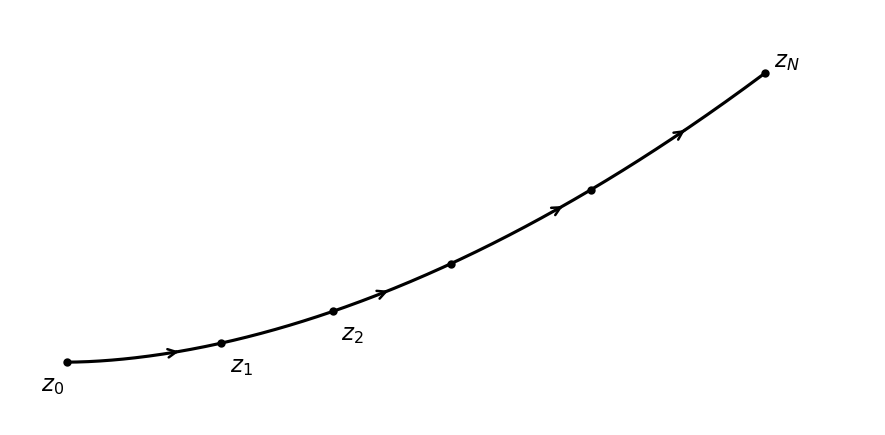
\includegraphics[width=10cm]{images/curve-z.png}

% [DUBBIO: figura con curva e punti z_0, z_1, z_N — non riproducibile]

il punto $z'_m$ giace sulla curva $C$ fra i punti $z_m$ e $z_{m-1}$, e $\Delta$ è la massima lunghezza del segmento di curva compreso fra due punti $z_m$ e $z_{m-1}$. Naturalmente, quando $\Delta$ tende a zero, il numero $N$ di intervalli in cui la curva $C$ è suddivisa diverge.

Se la curva $C$ è descritta dalla equazione parametrica (1), si ha ovviamente
\begin{equation}
\int_C dz\;f(z) = \int_{t_0}^{t_1} dt\;\frac{dz(t)}{dt}\;f[z(t)]\,, \tag{2}
\end{equation}
dove l'integrale a secondo membro è ora un integrale in senso ordinario (con integrando complesso, ma variabile di integrazione --- il parametro $t$ --- reale).

\noindent\rule{\linewidth}{0.4pt}

Il fatto di poter ridurre un integrale nel campo complesso ad un integrale ordinario (nel campo reale) ci permette di estendere immediatamente tutte le definizioni e nozioni relative alla convergenza di tale integrale, riconducendosi in ogni caso alla convergenza dell'integrale che compare a secondo membro della (2). Per esempio si dirà che l'integrale che compare a primo membro della (2) è assolutamente convergente, se è convergente
\[
\int_{t_0}^{t_1} dt\;\left|\frac{dz(t)}{dt}\right|\;\left|f[z(t)]\right|\,.
\]

\noindent\rule{\linewidth}{0.4pt}

Separando parte reale e parte immaginaria della funzione $f(z)$ ed esprimendole in funzione delle variabili $x$ ed $y$, rappresentanti la parte reale ed immaginaria di $z$, di modo che
\begin{align}
dz &= dx + i\,dy\,, \tag{3}\\
f(z) &= u(x,y) + i\,v(x,y)\,, \tag{4}
\end{align}

% === Pagina 415 (8.3-3) ===

si avrà inoltre
\begin{equation}
\int_C dz\;f(z) = \int_C \left[dx\;u(x,y) - dy\;v(x,y)\right] + i\int_C\left[dy\;u(x,y) + dx\;v(x,y)\right]\,, \tag{5}
\end{equation}
essendo gli integrali a secondo membro gli \underline{integrali curvilinei} lungo la curva $C$.

\noindent\rule{\linewidth}{0.4pt}

Si consiglia al lettore a questo punto di rinfrescarsi le idee --- ove ne avesse bisogno --- circa la definizione e le proprietà degli integrali curvilinei. Fra le proprietà, si ricorda in particolare il cosiddetto lemma di Gauss, secondo cui, se $C$ è una curva chiusa nel piano delle variabili $x$ e $y$,
\begin{align*}
\oint_C dx\; f(x,y) &= -\int dx\,dy\;\frac{\partial f(x,y)}{\partial y}\,, \\
\oint_C dy\; f(x,y) &= +\int dx\,dy\;\frac{\partial f(x,y)}{\partial x}\,,
\end{align*}
essendo gli integrali curvilinei a primo membro percorsi, lungo la curva chiusa $C$, in senso antiorario (cioè in modo da lasciare l'interno della curva a sinistra), e gli integrali bidimensionali a secondo membro essendo estesi a tutta la zona interna alla curva $C$.

\noindent\rule{\linewidth}{0.4pt}

Le seguenti proprietà seguono in modo ovvio dalla definizione di integrale nel campo complesso testé data:
\begin{align}
\tag{6} &\int_{-C} dz\; f(z) = -\int_C dz\; f(z) \\
\intertext{(dove con $-C$ si intende la stessa curva $C$, ma percorsa in senso inverso),}
\tag{7} &\int_{C_1} dz\; f(z) + \int_{C_2} dz\; f(z) = \int_{C_1+C_2} dz\; f(z)\,, \\
\tag{8} &\int_C dz\;\left[A\,f(z)\right] = A\int_C dz\; f(z)
\end{align}
se $A$ è una costante,
\begin{align}
\tag{9} &\int_C dz\left[f_1(z) + f_2(z)\right] = \int_C dz\; f_1(z) + \int_C dz\; f_2(z)\,, \\
\tag{10} &\left|\int_C dz\; f(z)\right| \leq \left|\int_C dz\;|f(z)|\right| \leq L\,M
\end{align}
dove $L$ è la lunghezza della curva $C$ ed $M$ è il massimo valore assunto dal modulo di $f(z)$ quando $z$ varia lungo la curva $C$.

La curva $C$ fin qui considerata potrebbe essere aperta o chiusa. Si suppone inoltre che sia regolare, o almeno che possa essere spezzata in un numero finito di tratti regolari. Nel caso di curve chiuse, si suppone per convenzione --- salvo esplicito contrario avviso --- che la curva venga percorsa in senso antiorario.

\noindent\rule{\linewidth}{0.4pt}

Una curva si dice \underline{regolare} se ammette in ogni punto una tangente ben definita; per esempio un cerchio è una curva regolare (chiusa), un triangolo è una curva chiusa ma non regolare (può però essere spezzato in tre curve regolari).

\noindent\rule{\linewidth}{0.4pt}

% === Pagina 416 (8.3-4) ===

Per esempio calcoliamo l'integrale
\begin{equation}
I = \int_C dz\;(z - z_0)^{-1}\,, \tag{11}
\end{equation}
essendo $z_0$ un numero complesso preassegnato ed essendo il contorno $C$ chiuso costituito da un cerchio di centro $z_0$ e raggio $\rho$ dato. La equazione parametrica di questa curva nel piano complesso è dunque
\[
z = z_0 + \rho\,e^{i\theta}\,, \quad \theta_0 \leq \theta \leq \theta_0 + 2\pi\,;
\]
l'intera curva viene infatti percorsa, dalla variabile $z$ data da questa equazione, al variare con continuità del parametro da un valore $\theta_0$ arbitrario (per esempio, $\theta_0 = 0$) fino a $\theta_0 + 2\pi$. Sarà dunque, per tale percorso
\begin{equation}
dz = i\rho\,e^{i\theta}\,d\theta = i(z - z_0)\,d\theta \tag{12}
\end{equation}
sicché
\begin{equation}
I = \int_C dz\;(z-z_0)^{-1} = i\int_0^{2\pi} d\theta = 2\pi i\,. \tag{13}
\end{equation}

Si noti che il valore dell'integrale non risulta dipendere dal raggio $\rho$ del cerchio; in effetti, come vedremo, l'integrale $I$ definito dalla (11) assume il valore (13) qualunque sia il contorno chiuso $C$, purché esso abbia la proprietà di circumnavigare (ed una sola volta) il punto $z_0$ (in senso antiorario).

Questo esempio è molto importante (vedi il paragrafo seguente).

L'integrazione nel campo complesso sin qui definita si applica a qualunque (ragionevole) funzione della variabile complessa $z$; in particolare, è chiaro che non si richiede che si tratti di una funzione analitica. Ma per le funzioni analitiche un importantissimo risultato è fornito dal seguente

\uline{Teorema di Cauchy}

\begin{teorema}[Cauchy]
Sia $w(z)$ una funzione analitica nel dominio semplicemente connesso $D$ del piano complesso $z$; sia $C$ una qualunque curva chiusa completamente inclusa in $D$; allora
\begin{equation}
\int_C dz\, w(z) = 0
\end{equation}
\end{teorema}

Un dominio si dice \underline{semplicemente connesso} se la sua frontiera è
costituita da una sola curva (senza soluzioni di continuità -- il che non esclude che la curva possa contenere punti angolosi). Si dice \underline{multiplamente connesso} se la sua frontiera è costituita da più curve distinte, non aventi punti in comune.

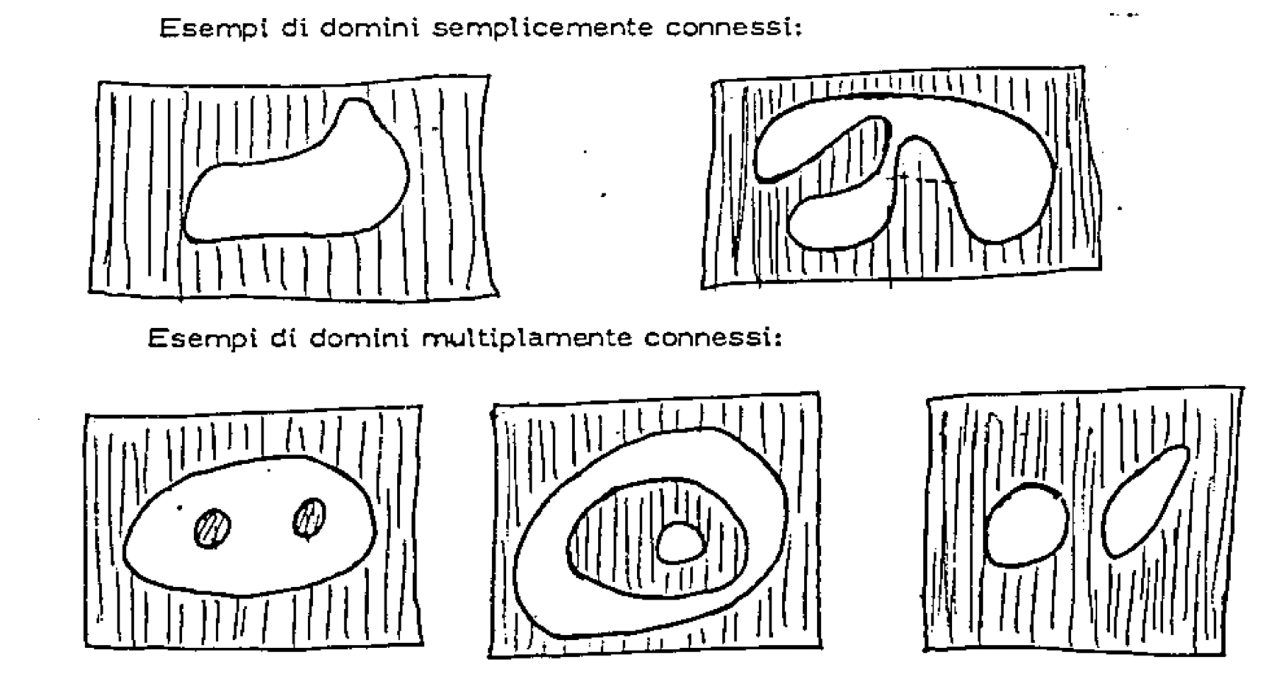
\includegraphics[width=15cm]{images/domini.png}




Dunque in parole povere l'integrale di qualunque funzione analitica su un contorno chiuso è nullo (attenzione: non basta però che la funzione sia analitica nelle vicinanze del contorno; occorre lo sia \underline{in tutta la zona interna al contorno}).

La dimostrazione del teorema di Cauchy è assai diretta. Usando il lemma di Gauss succitato e la definizione di integrale di variabile complessa (5), otteniamo

\begin{align}
\int_C dz\, w(z) &= \int dx\, dy \left[ -\frac{\partial u(x,y)}{\partial y} - \frac{\partial v(x,y)}{\partial x} \right] \notag \\
&\quad + i \int dx\, dy \left[ \frac{\partial u(x,y)}{\partial x} - \frac{\partial v(x,y)}{\partial y} \right] \tag{15}
\end{align}

gli integrali bidimensionali a secondo membro essendo estesi a tutta la regione del piano $xy$ inclusa dalla curva $C$. Ma se in ogni punto di tale regione la funzione $w(z)$ è analitica, cioè valgono le relazioni di Cauchy (1--5), gli integrandi sono identicamente nulli. È dunque nullo anche l'integrale nel campo complesso che compare a primo membro. C.V.D.

\medskip\hrule\medskip

Nell'enunciare il teorema di Cauchy si è assunto che il contorno $C$ fosse completamente interno al dominio $D$ entro cui la $w(z)$ è analitica. Ma è evidente che il risultato resta valido se anche il contorno $C$ coincide (in tutto o in parte) con la frontiera del dominio di analiticità di $w(z)$, purché su tale frontiera la $w(z)$ sia continua.

\medskip\hrule\medskip

Una immediata conseguenza del teorema di Cauchy è che, se la funzione $w(z)$ è analitica entro $D$, l'integrale di $w(z)$ esteso a qualunque curva (aperta) che abbia gli stessi estremi e sia completamente contenuta in $D$ ha lo stesso valore. (Infatti la differenza fra gli integrali percorsi lungo due diversi cammini, ambedue aventi lo stesso punto di inizio, $z_0$, e lo stesso punto terminale, $z$, è equivalente, grazie alla (6), all'integrale lungo la curva chiusa da $z_0$ a $z$ a $z_0$, ottenuta andando per un cammino e tornando per l'altro: per il teorema di Cauchy tale differenza è pertanto nulla).

Ciò porta a scrivere
\begin{equation}
W(z) = W(z_0) + \int_{z_0}^{z} dz'\, w(z') \tag{16}
\end{equation}
risultando l'integrale a secondo membro indipendente dal cammino di integrazione (è questo fatto che consente l'uso della notazione $\int_{z_0}^{z}$, che ricorda che il valore dell'integrale dipende dai punti estremi $z_0$ e $z$, ma non contiene invece alcuna indicazione del cammino). La funzione $W(z)$ che compare a primo membro, e che può essere considerata come definita da questa formula, sarà chiamata l'\underline{integrale indefinito} (o la \underline{primitiva}) della $w(z)$. È facile dimostrare che questa funzione è a sua volta analitica nello stesso dominio $D$ in cui è analitica la $W(z)$, e che vale la formula

\begin{equation}
W'(z) = w(z) \tag{17}
\end{equation}

(per convincersi della validità di questa formula -- che implica la validità della asserzione che la precede -- basta rifarsi alla definizione di integrale nel campo complesso data all'inizio di questa sezione).

È anche facile dimostrare che le consuete regole di integrazione continuano a valere nel campo complesso (per esempio, $\int_{z_0}^{z} dz'\, \cos(cz') = \left[\sin(cz) - \sin(cz_0)\right]/c$; etc.).

Un altro modo equivalente di esprimere il teorema di Cauchy è la affermazione che, se $w(z)$ è analitica, tanto la parte reale che la parte immaginaria della espressione
\begin{align}
w(z)\, dz &= \left[u(x,y)\, dx - v(x,y)\, dy\right] \notag \\
&\quad + i\left[u(x,y)\, dy + v(x,y)\, dx\right] \tag{18}
\end{align}
costituiscono dei \underline{differenziali esatti}, se considerati come forme differenziali nelle due variabili $x$ e $y$.

\medskip\hrule\medskip

Si ricordi che la forma differenziale
\[
X(x,y)\, dx + Y(x,y)\, dy
\]
costituisce un differenziale esatto se
\[
\frac{\partial X(x,y)}{\partial y} + \frac{\partial Y(x,y)}{\partial x} = 0\,;
\]
e si verifica subito che questa condizione, nel nostro caso, riproduce le condizioni di Cauchy (1--5).

Si ricordi inoltre che condizione necessaria e sufficiente perché una forma differenziale costituisca un differenziale esatto è che il suo integrale curvilineo, lungo tutte le curve aventi gli stessi punti di partenza e di arrivo, sia uguale: l'integrale curvilineo non dipende cioè dal cammino di integrazione, ma solo dagli estremi.

\medskip\hrule\medskip

Il teorema di Cauchy ci assicura dunque che qualunque integrale di una funzione di variabile complessa esteso ad una curva chiusa è nullo, se la curva è contenuta nel dominio di analiticità della funzione.

Ma la affermazione reciproca è anche vera, come risulta dal seguente \underline{Teorema di Morera}: se la $W(z)$ è una funzione continua della variabile complessa $z$ e l'integrale di $W(z)$ esteso a qualunque curva chiusa $C$ contenuta entro un dominio $D$ è nullo, allora la $w(z)$ è una funzione analitica della variabile complessa $z$ nel dominio $D$.

\medskip\hrule\medskip

\textit{Dimostrazione}: scelto arbitrariamente una volta per tutte un punto $z_0$ in $D$ si consideri l'integrale
\[
\int_{z_0}^{z} dz'\, w(z')
\]
percorso lungo un qualunque cammino tutto contenuto in $D$. Le ipotesi del teorema implicano che tale integrale non dipende dal particolare cammino scelto per andare da $z_0$ a $z$ (purché tale cammino sia incluso in $D$: infatti la differenza fra gli integrali percorsi lungo due diversi cammini è identica all'integrale lungo il cammino chiuso composto dal primo contorno, da $z_0$ a $z$, e dal secondo, da $z$ a $z_0$; è pertanto è nulla). Ma allora la forma differenziale $dz\, w(z)$ deve essere un differenziale esatto (nel piano delle variabili $x$ ed $y$, con $z = x + iy$); e, come abbiamo già visto, ciò implica che la parte reale e la parte immaginaria di $W(z)$ soddisfino alle relazioni di Cauchy (1--5); il che a sua volta implica che sia analitica. C.V.D.

\medskip

In conclusione il teorema di Cauchy implica, per ogni funzione $w(z)$ analitica in un dominio $D$, la possibilità di definire la funzione primitiva (o integrale indefinito) $W(z)$ che risulta anch'essa analitica in $D$, e la cui derivata coincide con $w(z)$. In sostanza si può dire che \underline{l'integrale di una funzione analitica è una funzione analitica}; come anche che \underline{la derivata di una funzione analitica è una funzione analitica} (per una dimostrazione, vedi la sezione seguente). E poiché l'operazione di integrazione, o differenziazione, si può ripetere più volte, se ne conclude che ogni funzione analitica è multiplamente integrabile, o ripetutamente differenziabile, quante volte si vuole, essendo sempre il risultato una funzione analitica (a condizione naturalmente che ci si mantenga sempre entro il dominio di analiticità $D$).

Prima di concludere questa sezione resta da menzionare una semplice, ma importantissima, estensione dell'enunciato dato sopra del teorema di Cauchy, estensione la cui validità segue immediatamente dalla dimostrazione del teorema di Cauchy stesso. Sottolineiamo anzitutto che si è finora assunto di avere a che fare con domini semplicemente connessi (e questa ipotesi è essenziale per la validità di alcuni dei risultati dati sino a questo punto). Nel caso invece di un dominio \underline{multiplamente connesso} $D$ entro cui la funzione $W(z)$ è analitica (e lo sia anche sulla frontiera del dominio stesso; o quanto meno sia continua sulla frontiera, il che basta per la validità del risultato), l'integrale di $W(z)$ sulla variabile complessa $z$, esteso all'\underline{intera} frontiera di $D$, è nullo, a condizione che il verso di percorrenza sia scelto in modo da lasciare la parte interna del dominio dalla stessa parte (convenzionalmente, a sinistra -- vedi figura)


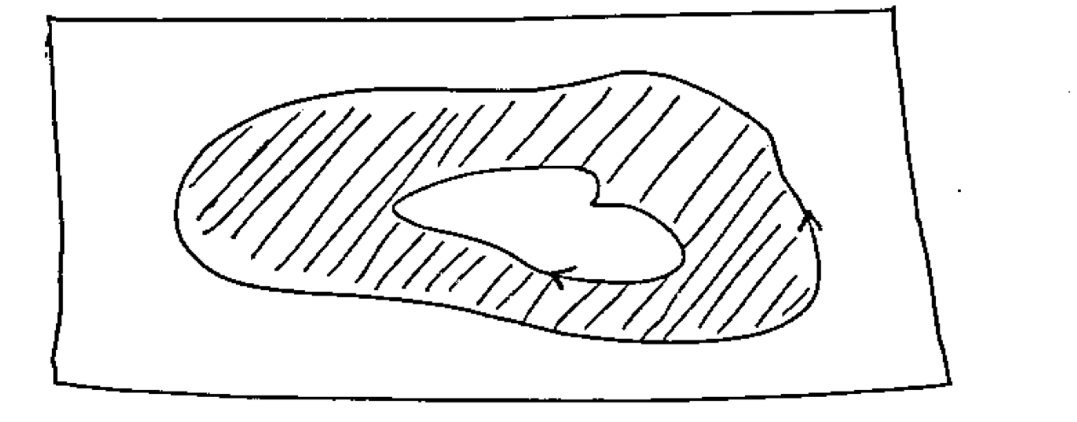
\includegraphics[width=13cm]{images/dominio_1.png}

\begin{esercizi}

\item La funzione $w(z)$ è analitica nel dominio multiplamente connesso indicato in figura. Si dimostri che l'integrale da $z_0$ a $z$ di $w(z)$ lungo un qualunque cammino $C$ non può dipendere dai dettagli del cammino $C$, ma solo dal numero di volte che il cammino $C$ gira intorno al buco (vedi figura; per esempio l'integrale lungo i due cammini indicati in figura dà necessariamente lo stesso risultato).

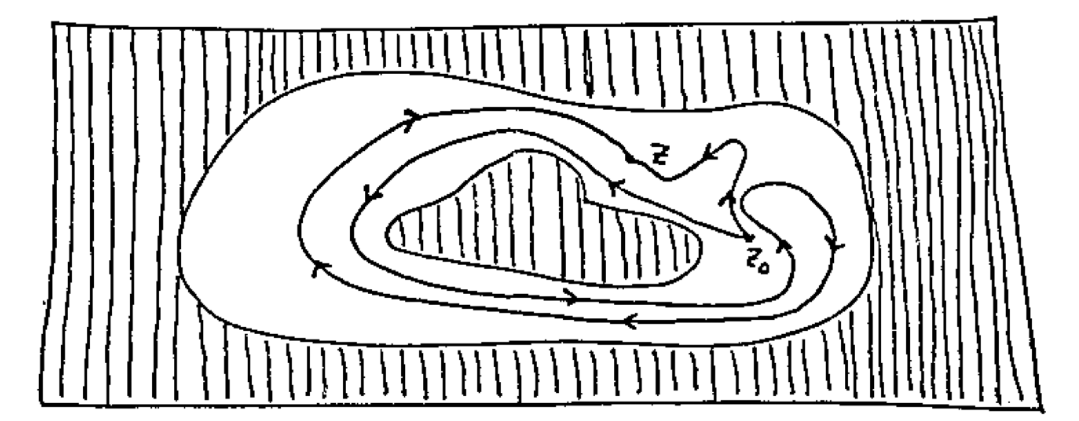
\includegraphics[width=13cm]{images/dominio_2.png}

\item Sia $C$ un contorno chiuso (senza incroci) nel piano complesso $z$, e sia $S$ l'area compresa entro $C$. Si dimostrino le seguenti formule
\[
\int_C x\, dz = i\, S\,,
\]
\[
\int_C y\, dz = -S\,,
\]
\[
\int_C z^*\, dz = 2i\, S\,,
\]
\[
\int_C z\, dz = 0\,.
\]
(In queste formule ovviamente $z \equiv x + iy$, e la curva $C$ si intende percorsa in senso antiorario).

\item Si calcoli l'integrale
\[
I_n = \int_C dz\, (z - z_0)^n\,, \quad n = 0, \pm 1, \pm 2, \pm 3, \ldots\,,
\]
essendo $C$ una curva chiusa includente il punto $z_0$ (e percorsa in senso antiorario).

\item Si calcolino gli integrali
\[
I_k = \int_{C_k} |z|^2\, dz\,, \quad k = 1, 2, 3\,,
\]
essendo la curva $C_1$ il segmento che congiunge il punto $z_0 = 0$ col punto $z = 1 + i$, la curva $C_2$ formata dai due segmenti da $0$ a $1$ a $1 + i$ e la curva $C_3$ dai due segmenti da $0$ a $i$ a $1 + i$.

\begin{center}
\begin{tikzpicture}[scale=2.2]
  \draw[->] (-0.15,0) -- (1.3,0) node[right] {};
  \draw[->] (0,-0.15) -- (0,1.3) node[above] {};
  % Punti
  \fill (0,0) circle (1pt) node[below left] {$O$};
  \fill (1,0) circle (1pt) node[below] {$1$};
  \fill (0,1) circle (1pt) node[left] {$i$};
  \fill (1,1) circle (1pt) node[above right] {$1+i$};
  % C1: diagonale
  \draw[->, thick] (0,0) -- (0.5,0.5);
  \draw[thick] (0.5,0.5) -- (1,1) node[midway, right] {$c_1$};
  % C2: da 0 a 1 poi a 1+i
  \draw[->, thick] (0,0) -- (0.5,0) node[midway, below] {$c_2$};
  \draw[thick] (0.5,0) -- (1,0);
  \draw[->, thick] (1,0) -- (1,0.5) node[midway, right] {$c_2$};
  \draw[thick] (1,0.5) -- (1,1);
  % C3: da 0 a i poi a 1+i
  \draw[->, thick] (0,0) -- (0,0.5) node[midway, left] {$c_3$};
  \draw[thick] (0,0.5) -- (0,1);
  \draw[->, thick] (0,1) -- (0.5,1) node[midway, above] {$c_3$};
  \draw[thick] (0.5,1) -- (1,1);
\end{tikzpicture}
\end{center}

\item Nell'assunto del teorema di Morera si è introdotta l'ipotesi che la funzione $w(z)$ sia continua; la dimostrazione è poi stata solo accennata, sicché non è risultato evidente il ruolo di tale ipotesi. È questa ipotesi essenziale per la validità del teorema?

\textit{Suggerimento}: si osservi che esempi forniti precedentemente (vedi per esempio l'esercizio 3) configurano il caso di funzioni non ovunque analitiche ma il cui integrale su curve \underline{chiuse} è nullo.

\end{esercizi}

\section{Rappresentazione integrale di Cauchy di una funzione analitica e delle sue derivate}

Sia la $w(z)$ una funzione analitica nel dominio $D$, sia $z$ un punto interno a $D$, e $C$ una curva contenuta in $D$ (o coincidente, in tutto o in parte, con la frontiera di $D$, nella ipotesi che la $w(z)$ sia continua sulla frontiera di $D$). Vale allora la formula (\underline{rappresentazione integrale di Cauchy})
\begin{equation}
w(z) = \frac{1}{2\pi i} \int_C dz'\, w(z') / (z' - z) \tag{1}
\end{equation}
nella ipotesi che il punto $z$ sia \underline{interno} alla curva $C$ e che il percorso $C$ venga percorso in senso antiorario (si noti che, se $z$ fosse esterno a $C$, per il teorema di Cauchy l'integrale a secondo membro darebbe un risultato nullo).

\medskip\hrule\medskip

Diamo della rappresentazione di Cauchy una dimostrazione un po' sbrigativa. Scriviamo
\begin{align*}
\frac{1}{2\pi i} \int_C dz'\, w(z')/(z'-z)
&= \frac{1}{2\pi i} \int_C dz' \left\{ \left[w(z')-w(z)\right]+w(z) \right\}/(z'-z) \\
&= \frac{1}{2\pi i} \int_C dz' \left[w(z')-w(z)\right]/(z'-z) \\
&\quad + \frac{w(z)}{2\pi i} \int_C dz'/(z'-z) \\
&= w(z)\,.
\end{align*}
L'ultimo passaggio è stato effettuato utilizzando il teorema di Cauchy per affermare che il primo integrale è nullo (l'integrando risulta analitico entro $C$, essendo cancellata dall'annullarsi del numeratore la singolarità derivante dall'annullarsi del denominatore), ed utilizzando la (13) per valutare il secondo integrale.

La dimostrazione è ``sbrigativa'' perché la cancellazione della singolarità, che giustifica l'uso del teorema di Cauchy, andrebbe accertata più rigorosamente; si lascia al lettore di fare questa verifica, utilizzando il teorema di Cauchy per ridurre il cammino $C$ ad un cerchio di piccolo raggio $\rho$ intorno a $z$, e dimostrando poi che l'integrale si annulla nel limite $\rho \to 0$.

\medskip\hrule\medskip

La formula (1) è assai notevole, in quanto mostra come il valore della funzione analitica $w$ nel punto $z$ sia legato ai valori che la stessa funzione assume su un qualunque contorno che circonda il punto $z$. Questa proprietà abbastanza straordinaria indica che i valori di una funzione analitica in diverse zone del piano complesso non possono essere assegnati arbitrariamente, ma sono in qualche modo correlati. In effetti vedremo nella prossima sezione come la conoscenza dei valori di una funzione analitica della variabile complessa $z$ in un intorno, anche piccolissimo, di un punto $z_0$, sia sufficiente a determinare (tutt'al più non univocamente) i valori della funzione negli altri punti del piano complesso.

Un semplice corollario del teorema di Cauchy fornisce una diretta illustrazione della possibilità di esprimere una funzione analitica in un punto tramite i valori che essa assume in un intorno di tale punto. Tale corollario è la formula
\begin{equation}
w(z) = \frac{1}{2\pi} \int_0^{2\pi} d\theta\, w\!\left[z + \rho\, e^{i\theta}\right] \tag{2}
\end{equation}
valida a condizione che la funzione $w$ sia analitica entro un cerchio di centro $z$ e raggio $\rho$. Questa formula segue infatti dal teorema di Cauchy scegliendo come contorno tale cerchio.

Utilizzando il corollario (2) è facile dimostrare il seguente teorema, che esprime un'altra sorprendente proprietà delle funzioni analitiche: \underline{se una funzione è analitica entro un dominio $D$ ed è continua sulla frontiera di $D$, il valore massimo (o i valori massimi) del modulo di tale funzione vengono necessariamente assunti sulla frontiera di $D$} (\underline{principio del massimo modulo di una funzione analitica}), salvo il caso banale in cui la funzione si riduce ad una costante.

\medskip\hrule\medskip

Lasciando la rigorosa dimostrazione di questo risultato come esercizio per il lettore, vogliamo qui renderlo plausibile (indicando nello stesso tempo la via per una dimostrazione rigorosa). Il teorema afferma in sostanza che, se si facesse il grafico bidimensionale (o meglio, il ``rilievo altimetrico'') della funzione $|w(z)|$, riportandone il valore in altezza al disopra del piano cartesiano $xy$ in corrispondenza ad ogni valore della variabile complessa $z = x + iy$, tale rilievo non potrebbe mai avere un colle entro la zona in cui la funzione $w(z)$ è analitica; cioè non vi può essere alcun punto interno al dominio di analiticità della funzione $w(z)$ in cui il modulo $|w(z)|$ raggiunga il massimo rispetto a tutti i punti circostanti. Che questo non possa accadere è infatti conseguenza della (2), che ovviamente implica anche
\[
|w(z)| \leq \frac{1}{2\pi} \int_0^{2\pi} d\theta\, \left|w\!\left[z + \rho\, e^{i\theta}\right]\right|
\]

% [DUBBIO: "o minore" scritto a mano sopra la riga, probabilmente è una nota marginale del professore che precisa che il modulo è minore o uguale alla media]

cioè che il modulo di $w$ nel punto $z$ sia pari al valor medio del modulo di $w$ in un cerchio intorno a $z$. Ci dovrà dunque essere, a partire da qualunque punto interno al dominio di analiticità di $w(z)$, qualche direzione in cui $|w(z)|$ cresce (e, salvo per i punti in cui $w(z) = 0$ e dunque $|w(z)| = 0$, anche qualche direzione in cui $|w(z)|$ cresce; vedi sotto).

Ne segue che, considerato qualunque dominio $D$ entro cui $w(z)$ è analitica, i punti in cui $|w(z)|$ assume il valore massimo non possono cedere che sulle frontiere di $D$, come il teorema per l'appunto afferma.

\medskip\hrule\medskip

È chiaro che, se la funzione $W(z)$ è analitica in $D$ e non si annulla, anche la funzione $\nu(z) = 1/W(z)$ è analitica in $D$. Applicando il teorema testé discusso a $\nu(z)$ possiamo pertanto concludere che vale anche il \underline{principio del minimo modulo di una funzione analitica} (e che non si annulli), secondo cui \underline{se una funzione $w(z)$ è analitica e non si annulla in $D$, i minimi valori del modulo di $w(z)$ (come anche i massimi valori del modulo di $w(z)$) sono necessariamente assunti sulla frontiera di $D$}.

Tornando ora alla rappresentazione di Cauchy (1), osserviamo che si tratta di un caso particolare di \underline{rappresentazione integrale di una funzione}, consistendo questa in una formula del tipo
\begin{equation}
W(z) = \int_C dz'\, \nu(z, z') \tag{3}
\end{equation}
Qui $W(z)$ è la funzione rappresentata, $\nu(z, z')$ è una funzione di due variabili complesse supposta nota, e $C$ è una curva (aperta o chiusa) nel piano della variabile complessa, che anche si suppone sia assegnata. Rappresentazioni di questo tipo sono particolarmente utili nel caso di funzioni analitiche (in particolare, quando la $\nu(z, z')$ sia una funzione analitica della variabile $z'$), perché allora, utilizzando il teorema di Cauchy, si può deformare il cammino di integrazione e in tal modo passare da una rappresentazione ad un'altra, che può essere più conveniente per mettere in luce particolari proprietà della funzione $W(z)$, o permetterne una valutazione approssimata.

È inoltre assai interessante il caso in cui $\nu(z, z')$ sia una funzione analitica di $z$, caso in cui ci si può attendere che $W(z)$ sia anche una funzione analitica di $z$, purché questa proprietà non vada perduta nella integrazione sulla variabile $z'$ (e ciò dipenderà ovviamente dalle proprietà di $\nu(z, z')$ quando $z'$ varia lungo la curva $C$). A questo proposito vale il seguente teorema: se la funzione $\nu(z, z')$ è una funzione analitica di $z$ entro un dominio $D$ per ogni valore di $z'$ sulla curva (di lunghezza finita) $C$, e se $\nu(z, z')$ e la derivata $\partial\nu(z,z')/\partial z$ (per $z'$ fisso su $C$; questa derivata esiste poiché $\nu(z,z')$ è per ipotesi funzione analitica di $z$ per $z'$ su $C$) dipendono in modo continuo da $z$ e da $z'$ per ogni variazione di $z$ entro $D$ e di $z'$ su $C$, allora la funzione $W(z)$ definita dalla (3) è una funzione analitica della variabile complessa $z$, e la derivata $w'(z)$ di questa funzione rispetto alla variabile complessa $z$ può essere ottenuta differenziando sotto segno di integrale, cioè
\begin{equation}
\frac{dW(z)}{dz} = \int_C dz'\, \frac{\partial\nu(z,z')}{\partial z} \tag{4}
\end{equation}

\medskip\hrule\medskip

Questo teorema non ha nulla di sorprendente, e non riteniamo sia il caso di attardarci a darne una esplicita dimostrazione, limitandoci ad indicare che la si potrebbe basare sulla possibilità di scambiare le operazioni di integrazione e differenziazione nel caso di funzioni di due variabili, e i integrali curvilinei (per il che si richiede l'esistenza e continuità delle derivate parziali dei coefficienti della forma differenziale), e sulla identità di Cauchy (1--5).

Sarà però bene sottolineare che il teorema testé enunciato si riferisce a curve $C$ di \underline{lunghezza finita}. Nel caso di curve di lunghezza infinita può infatti verificarsi il caso che, per certi valori di $z$, l'integrale a secondo membro della (3) cessi di convergere. Ciò non implica necessariamente che la funzione $W(z)$ sia, in corrispondenza a tali valori di $z$, non analitica (singolare); si può solo concludere che la rappresentazione integrale (3) cessa, per tali valori di $z$, di valere, non fornendo più alcuna informazione sui valori della $W(z)$ o sulle sue proprietà di analiticità.

Quasi immediata conseguenza del teorema testé enunciato è la rappresentazione di Cauchy per la derivata ennesima di una funzione analitica, fornita dalla formula
\begin{equation}
\frac{d^n W(z)}{dz^n} \equiv W^{(n)}(z) = \frac{n!}{2\pi i} \int_C dz'\, w(z') / (z'-z)^{n+1} \tag{5}
\end{equation}
che è valida sotto le stesse ipotesi della (1), e che ovviamente segue da questa differenziando sotto il segno di integrale. Questa formula implica naturalmente l'esistenza di tutte le derivate di una funzione analitica in ogni punto interno al suo dominio di analiticità, e ne fornisce inoltre una esplicita rappresentazione in funzione dei valori che la funzione stessa assume su una qualunque curva chiusa includente il punto $z$ e tutta contenuta in $D$ (o eventualmente coincidente con la frontiera di $D$, purché la $W(z)$ si mantenga ivi continua).

Terminiamo questa sezione con il \underline{teorema di Liouville}, secondo cui \underline{se una funzione è analitica in tutto il piano complesso, ed è inoltre limitata in modulo (in tutto il piano complesso), essa è necessariamente una costante.}

\medskip\hrule\medskip

\textit{Dimostrazione}: dalla (5) segue
\[
w'(z) = \frac{1}{2\pi i} \int_C dz'\, w(z') / (z'-z)^2\,,
\]
essendo la curva $C$ una qualunque curva che circonda (in senso orario) il punto $z$. Nella ipotesi del teorema, secondo cui esiste un numero $M$ tale che, per ogni $z$,
\[
|w(z)| < M\,,
\]
dalla relazione scritta segue ovviamente (vedi la (8-10))
\[
|w'(z)| \leq \frac{M}{2\pi} \left| \int_C dz'\, |z'-z|^{-2} \right|\,.
\]
Scegliendo come cammino di integrazione un cerchio di raggio $\rho$ intorno al punto $z$, da questa si ottiene
\[
|w'(z)| < M/\rho\,,
\]
e poiché $\rho$ si può scegliere arbitrariamente grande, ne segue che $|w'(z)|$ è minore di un numero arbitrariamente piccolo, il che è possibile solo se
\[
|w'(z)| = 0\,.
\]
Ma se, per ogni $z$, $w'(z) = 0$, ne segue che $w(z) = \text{costante}$, che è appunto quel che si doveva dimostrare.

\medskip\hrule\medskip

Una funzione che sia analitica in tutto il piano complesso si dice \underline{intera}. Il teorema di Liouville assicura dunque che, a parte il caso banale delle costanti, tutte le funzioni intere necessariamente divergono in modulo per $|z| \to \infty$ in qualche direzione del piano complesso (si noti che le funzioni intere, essendo analitiche, sono necessariamente limitate per ogni valore finito di $z$). Esempi di funzioni intere sono i polinomi, la funzione esponenziale, le funzioni circolari (seno e coseno); si noti che anche queste divergono in modulo, per $|z| \to \infty$ lungo l'asse immaginario.

\begin{esercizi}

\item Si calcoli il valore dei seguenti integrali, tutti estesi ad un cerchio di raggio $\rho = 1$, centrato nell'origine del piano complesso e percorso in senso antiorario:
\begin{align*}
I_1 &= \int_C dz\, z^2/(z-2) \\
I_2 &= \int_C dz\, z^2/(2z-1) \\
I_3 &= \int_C dz\, z^3/(2iz+1) \\
I_4 &= \int_C dz\, e^{iz}/z^3 \\
I_5 &= \int_C dz\, (z-2)^{-2}(2z-1)^{-1}\,, \quad
I_6 = \int_C dz\, (z-2)^{-1}(2z-1)^{-2}\,.
\end{align*}
Quale dei risultati cambia (e come*) se, invece di $\rho = 1$, si avesse $\rho = 3$?

\item Si dimostri che, se $P_n(z)$ è un polinomio di grado $n$ in $z$, ed $N$ è un intero maggiore di $n+1$, l'integrale
\[
\int_C dz\, P_n(z)/(z-z_0)^{N+1}
\]
su qualunque curva chiusa non passante per il punto $z_0$, è nullo.

\item Si calcoli il valore massimo che la funzione $w(z) = |\sin z|$ assume in un quadrato del piano complesso $z$ avente per vertici i quattro punti di coordinate $z = \pm a \pm ia$, con $a$ costante reale (positiva).

\end{esercizi}

\section{Sviluppo in serie di Taylor. Continuazione analitica. Funzioni monodrome e polidrome.}

Nella precedente sezione abbiamo stabilito la rappresentazione di Cauchy per una funzione analitica e per tutte le sue derivate, rappresentazione sintetizzabile nella formula
\begin{equation}
W^{(n)}(z) = \frac{n!}{2\pi i} \int_C dz'\, w(z') / (z'-z)^{n+1} \tag{1}
\end{equation}
con $W^{(n)}(z) \equiv d^n w(z)/dz^n$, $n = 0, 1, 2, \ldots$

In questa formula il contorno chiuso $C$ si intende, come al solito, che sia percorso in senso antiorario; deve inoltre essere tale da includere il punto $z$ e da escludere ogni (eventuale) singolarità di $w(z)$, occorre cioè che $w(z')$ sia analitica per ogni valore di $z'$ che cada all'interno di $C$ (o su $C$; in effetti è sufficiente che $W(z)$ sia continua su $C$ o più precisamente per $z$ che raggiunge $C$ dall'interno).

\medskip

La terminologia precedente fa riferimento al caso di domini semplicemente connessi. In effetti il risultato vale anche per domini multiplamente connessi, nel qual caso la curva $C$ rappresenterà l'intero contorno del dominio e andrà percorsa in modo da lasciare a sinistra la parte interna del dominio; e alla funzione $w(z)$ si richiederà (naturalmente) di essere analitica nel dominio. Per esempio per una funzione analitica nel dominio anulare del piano complesso caratterizzato dalla formula $z = \rho\, e^{i\theta}$ con $\rho_1 \leq \rho \leq \rho_2$ e $0 \leq \theta < \pi$, la rappresentazione (1) vale per ogni $z$ contenuta nell'anello, essendo la curva $C$ composta dai due cerchi di raggio $\rho_1$ e $\rho_2$, il primo percorso in senso orario e il secondo in senso antiorario (fare figura!).

Nel seguito per semplicità di linguaggio, ipotizzeremo di avere a che fare con un dominio semplicemente connesso, lasciando al lettore la ovvia generalizzazione al caso multiplamente connesso.

\medskip\hrule\medskip

Per $n=0$, la (1) si riduce alla rappresentazione di Cauchy
\begin{equation}
w(z) = \frac{1}{2\pi i} \int_C dz'\, w(z') / (z'-z)\,. \tag{2}
\end{equation}

Mostriamo ora come da questa formula se ne ottenga un'altra, esprimente la $w(z)$ come serie di potenze in $z-z_0$ (\underline{sviluppo in serie di Taylor} nell'intorno del punto $z_0$).

Sia dunque $z_0$ un punto interno alla curva $C$, e sia $\rho$ il raggio di un cerchio centrato in $z_0$ e completamente interno al dominio racchiuso dalla curva $C$:

\begin{center}
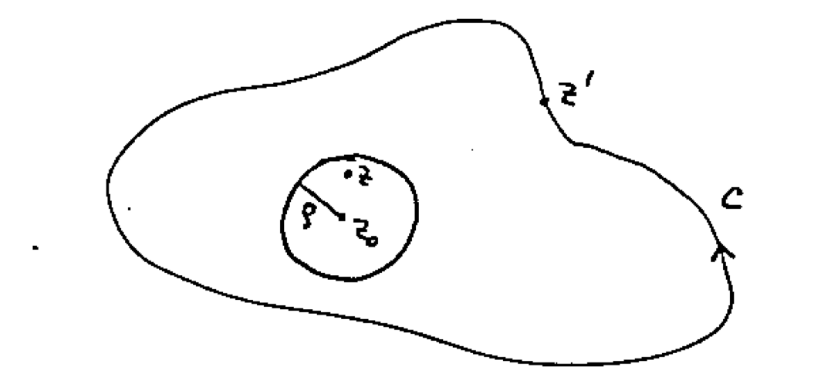
\includegraphics[width=10cm]{images/dominio_3.png}
\end{center}

Sia $z$ un punto interno a tale cerchio; $z$ sarà allora anche interno a $C$, e dunque la rappresentazione (2) (nonché la (1)) saranno valide. Inoltre per ogni $z'$ su $C$ varrà la relazione
\begin{equation}
|(z-z_0)/(z'-z_0)| \equiv |(z-z_0)|/|z'-z_0| < 1\,. \tag{3}
\end{equation}

\medskip\hrule\medskip

Si veda la figura qui sopra, e si ricordi che le ipotesi fatte sinora implicano $|z-z_0| < \rho$ e $|z'-z_0| > \rho$.

\medskip\hrule\medskip

Pertanto per ogni $z'$ su $C$, e per ogni $z$ entro il cerchio di raggio $\rho$ e centro $z_0$, la serie geometrica
\[
\sum_{n=0}^{\infty} \left[(z-z_0)/(z'-z_0)\right]^n
\]
risulta assolutamente convergente al valore
\begin{equation}
\left[1-(z-z_0)/(z'-z_0)\right]^{-1} = (z'-z_0)/(z'-z)\,, \tag{4}
\end{equation}
sicché possiamo scrivere
\begin{equation}
(z'-z)^{-1} = \sum_{n=0}^{\infty} (z-z_0)^n / (z'-z_0)^{n+1}\,. \tag{5}
\end{equation}
La convergenza della serie a secondo membro è inoltre uniforme in $z'$, per ogni $z'$ su $C$.

Ma allora possiamo sostituire la (5) nella (2), invertire l'ordine delle operazioni di integrazione e di somma, ed usare la (1), ottenendo
\begin{equation}
W(z) = \sum_{n=0}^{\infty} c_n\, (z-z_0)^n \tag{6}
\end{equation}
con
\begin{equation}
c_n = W^{(n)}(z_0) / n!\,. \tag{7}
\end{equation}
È questo lo sviluppo cercato. Si noti che la derivazione testé effettuata ne garantisce la assoluta e uniforme convergenza, a condizione che la funzione $w(z)$ sia analitica in $z_0$, e la variabile $z$ cada entro un cerchio di centro $z_0$ e tale che, per ogni punto interno a tale cerchio, la $w(z)$ sia analitica.

Si noti che l'esistenza dei coefficienti $c_n$ è garantita dalla analiticità della $w(z)$ in $z_0$, che a sua volta garantisce l'esistenza di tutte le derivate della $W(z)$ nel punto $z_0$. In effetti analiticità di una funzione di variabile complessa in un punto, e sviluppabilità in serie di Taylor nell'intorno di quel punto, sono concetti equivalenti.

Come si è visto, la convergenza dello sviluppo di Taylor è ``per cerchi''; si ha cioè convergenza entro ogni cerchio centrato in $z_0$ e di raggio $\rho$ sufficientemente piccolo; se si fa aumentare $\rho$, cioè si espande il cerchio intorno al punto $z_0$, la convergenza cesserà di valere se e quando la circonferenza incontrerà una singolarità di $w(z)$, un punto cioè in cui $w(z)$ non è analitica. Si potrà dunque affermare che lo sviluppo in serie di Taylor della funzione $w(z)$ nell'intorno del punto $z_0$ converge entro un cerchio del piano complesso $z$ di centro $z_0$ e di raggio pari alla distanza $d = |z_0 - z_s|$ di $z_0$ dal punto singolare $z_s$ di $w(z)$ più vicino a $z_0$ stesso.

A tale distanza si fa riferimento come al ``raggio di convergenza'' dello sviluppo di Taylor della funzione $w(z)$ nel punto $z_0$.

Per le funzioni intere, cioè prive di singolarità per ogni valore (finito) di $z$, lo sviluppo in serie di Taylor avrà raggio di convergenza infinito, convergerà cioè per ogni valore finito della variabile $z$ (qualunque sia il punto $z_0$ nel cui intorno si esegue lo sviluppo).

La uniforme e assoluta convergenza dello sviluppo in serie di Taylor permette, entro il cerchio di convergenza, di scambiare l'ordine delle operazioni di differenziazione o di integrazione con l'operazione di somma. Sicché se vale la formula
\begin{equation}
W(z) = \sum_{n=0}^{\infty} c_n\, (z-z_0)^n \tag{8}
\end{equation}
sarà anche
\begin{equation}
dW(z)/dz = \sum_{n=0}^{\infty} n\, c_n\, (z-z_0)^{n-1} \tag{9}
\end{equation}
e
\begin{equation}
\int_{z_1}^{z_2} dz\, W(z) = \sum_{n=0}^{\infty} c_n \left[(z_2-z_0)^{n+1} - (z_1-z_0)^{n+1}\right]/(n+1)\,, \tag{10}
\end{equation}
a condizione beninteso di mantenersi sempre entro il cerchio di convergenza.

Abbiamo già indicato che lo sviluppo in serie di Taylor potrebbe essere preso come punto di partenza dell'intera teoria delle funzioni analitiche. Sottolineiamo ora che esso ha una implicazione profonda circa la natura delle funzioni analitiche; mostra infatti che, se una funzione analitica è nota in un intorno, per quanto piccolo, di un punto, essa risulta determinata ovunque. Infatti basta che sia nota in un intorno, per quanto piccolo, del punto $z_0$, perché siano univocamente determinate tutte le sue derivate, quindi i coefficienti del suo sviluppo di Taylor, quindi la funzione stessa entro un cerchio il cui raggio è pari alla distanza da $z_0$ della singolarità della funzione più vicina a $z_0$ stesso. E in generale, se tale singolarità è isolata, i valori della funzione risultano determinati anche al di fuori di tale cerchio di convergenza, in quanto la funzione può essere di nuovo sviluppata nell'intorno di un altro punto $z_1$ interno al cerchio di convergenza centrato in $z_0$. Il nuovo cerchio di convergenza, centrato in $z_1$, includerà infatti anche una zona che è al di fuori del primitivo cerchio di convergenza centrato in $z_0$. E il procedimento può essere continuato, permettendo generalmente di definire la funzione in tutto il piano complesso.

A questo procedimento, che permette di estendere una funzione analitica, originariamente definita in una regione del piano complesso, al di fuori di tale zona, si dà il nome di \underline{continuazione analitica}. Al particolare meccanismo di continuazione analitica basato sulla serie di Taylor testé descritto è associato il nome del matematico tedesco Weierstrass. Esso è forse illustrato, meglio che dalla precedente descrizione, dalla seguente figura:

\begin{center}
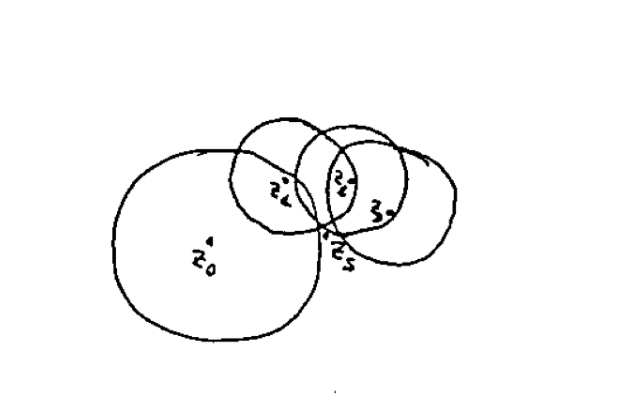
\includegraphics[width=10cm]{images/cerchi_1.png}
\end{center}

in cui $z_0, z_1, z_2, \ldots$ sono i successivi punti in cui si immagina di sviluppare la funzione in serie di Taylor e $z_s$ è per ipotesi l'unico punto di singolarità della funzione che si sta considerando. Si noti che la funzione avrebbe potuto essere inizialmente definita solo in un piccolissimo intorno del punto $z_0$, risultando poi definita entro tutta la zona coperta dai cerchi (e naturalmente il procedimento potrebbe continuare).

Non è detto che con questo metodo si possa continuare ovunque una funzione analitica; potrebbe darsi che questa risulti definita entro una certa zona, circondata da una barriera ininterrotta di singolarità. In questo caso si dice che la funzione ammette un \underline{confine naturale} di analiticità. Ma funzioni di questo tipo sono eccezionali, nel senso che in pratica non si presentano mai nella soluzione di problemi fisici.

\medskip\hrule\medskip

Un esempio di funzione di questo tipo è definita dalla serie
\[
W(z) = \sum_{n=1}^{\infty} z^{n!}
\]
(si noti che questa è in effetti una serie di Taylor nell'intorno di $z_0 = 0$, ma con tanti coefficienti nulli, essendo presenti -- con coefficiente pari ad $1$ -- solo i termini con esponente esprimibile come $n!$). È ovvio che questa serie converge per $|z| < 1$, poiché

chiaramente
\[
|w(z)| \leq \sum_{n=1}^{\infty} |z|^{n!} < \sum_{m=1}^{\infty} |z|^m
\]
e l'ultima serie converge (al valore $|z|/(1-|z|)$) per $|z|<1$. Ma è anche facile mostrare che la serie che definisce $w(z)$ diverge per ogni valore di $z$ che possa essere espresso nella forma
\[
z = e^{2i\pi\ell/m}
\]
con $\ell$ ed $m$ interi. Infatti in corrispondenza a tali valori di $z$, la $w(z)$ si riduce a
\[
w(z) = \sum_{n=1}^{\infty} e^{2i\pi\ell\, n!/m}
\]
e le serie a secondo membro di questa formula divergono evidentemente, poiché per $n \geq m$ tutti gli addendi prendono la forma $e^{2i\pi N}$ con $N$ intero, sono cioè pari ad $1$. Dunque la serie che definisce la $w(z)$ per $|z|<1$ diverge per ogni valore di $z$ del tipo $z = e^{2\pi i\ell/m}$ con $\ell$ ed $m$ interi; la arbitrarietà di questi due numeri mostra che, scelto comunque un punto sulla circonferenza $|z|=1$, esistono altri punti del cerchio in cui la serie diverge e che sono vicini quanto si vuole al punto dato. Per questa funzione il cerchio di equazione $|z|=1$ costituisce dunque un confine naturale di analiticità, e la funzione non può essere continuata analiticamente al di fuori del disco $|z|<1$.

\medskip\hrule\medskip

Normalmente le singolarità di una funzione analitica -- cioè i punti in cui cadono in difetto le relazioni di Cauchy, la funzione o le sue derivate non risultano definite, lo sviluppo in serie di Taylor cessa di convergere -- sono invece dei punti isolati, e dunque possono essere aggirate con la tecnica di continuazione analitica testé descritta (o con un'altra tecnica equivalente di continuazione analitica, vedi sotto); e in questo modo a partire da un intorno piccolo quanto si vuole, di un punto di analiticità, si può continuare analiticamente la funzione in tutto il piano complesso (cioè, costruire una funzione analitica definita in tutto il piano complesso e che coincide con la funzione originaria nella zona in cui questa era stata inizialmente assegnata).

La tecnica di continuazione analitica ora descritta fornisce dunque il valore della funzione in qualunque punto $z$, tramite una successione di dischi parzialmente sovrapposti e disposti in modo da evitare eventuali singolarità della funzione, successione che costruisce un corridoio ininterrotto a partire dal disco iniziale centrato in $z_0$. È ovvio che uno stesso punto può essere raggiunto con diverse catene di dischi: il valore delle funzioni in $z$ ottenuto seguendo l'una o l'altra strada, deve necessariamente essere lo stesso o può essere diverso?

\begin{center}
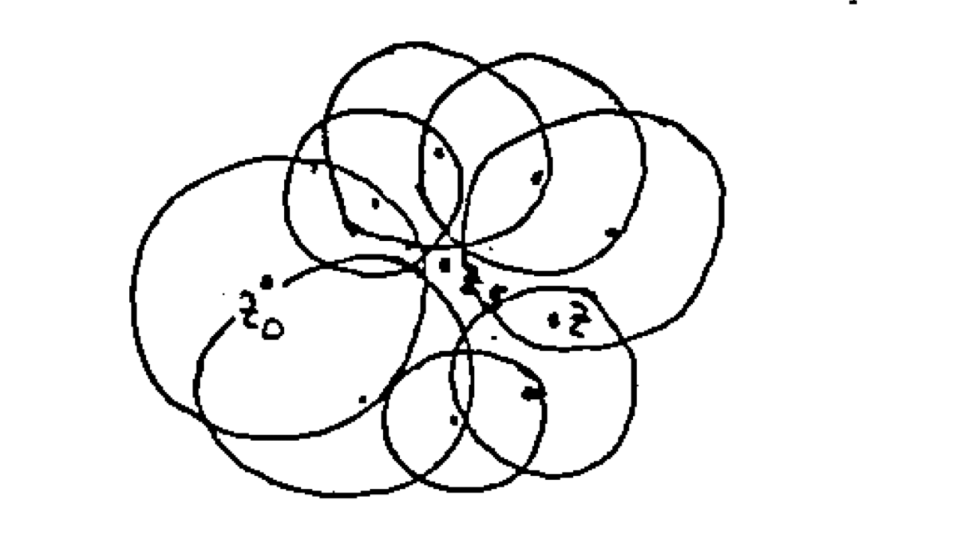
\includegraphics[width=10cm]{images/cerchi_3.png}
\end{center}

È anzitutto chiaro che, se i due cammini sono tali che, andando per l'uno e tornando per l'altro, non resti inclusa dentro il contorno chiuso così ottenuto nessuna singolarità della funzione, allora i valori della $W(z)$ in $z$ inizialmente ottenuti tramite le due continuazioni analitiche debbono necessariamente coincidere.

\medskip\hrule\medskip

È questa una conseguenza del teorema di Cauchy, applicato alla derivata $w'(z)$ della $W(z)$, che naturalmente sarà a sua volta definita, ed analitica, in ogni punto in cui è definita per continuazione analitica la $W(z)$. Infatti sarà:
\[
W(z) = W(z_0) + \int_C dz'\, w'(z')\,,
\]
dove il cammino $C$ va da $z_0$ a $z$. Scegliendo il cammino entro l'uno o l'altro dei corridoi forniti dalla successione di dischi (vedi per esempio le curve $C_1$ e $C_2$ nella figura disegnata sopra) si otterrebbero dunque due diverse determinazioni della funzione $W(z)$; la differenza tra tali due determinazioni coincide con la differenza tra i due integrali della $w'(z)$, percorsi lungo i due cammini $C_1$ e $C_2$; equivalentemente, tale differenza coincide con l'integrale di $w'(z)$ lungo il contorno chiuso costituito dalla curva $C_1$ (percorsa da $z_0$ a $z$) e la curva $C_2$ (percorsa da $z$ a $z_0$); è dunque nulla per il teorema di Cauchy, se $W(z)$, e dunque anche $w'(z)$, non contiene nessuna singolarità entro il contorno $C$.

Si noti che in questo caso il procedimento di continuazione analitica alla Weierstrass permetterebbe di ricoprire di dischi l'intera zona inclusa tra i due corridoi (vedi ancora la figura disegnata qui sopra; % [DUBBIO: nota manuale "si utilizzerà lo spazio bianco per ridisegnarla meglio con un compasso!"]
).

\medskip\hrule\medskip

Nel caso invece in cui i due diversi corridoi che conducono dal punto $z_0$ al punto $z$ includano una, o più, singolarità della funzione $W(z)$, è possibile che le due determinazioni della funzione ottenuta eseguendo la continuazione analitica lungo i due cammini forniscano valori diversi:

\begin{center}
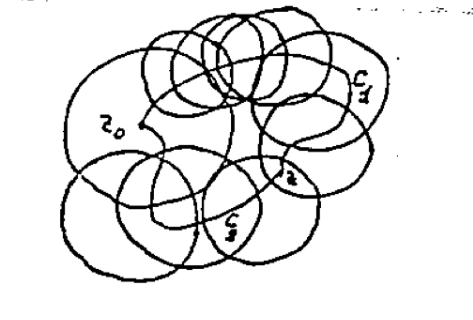
\includegraphics[width=10cm]{images/cerchi_2.png}
\end{center}

Se questo avviene, si ha a che fare con funzioni analitiche \underline{polidrome}; se ciò non avviene, la funzione $W(z)$ è invece \underline{monodroma}. Ambedue queste possibilità possono verificarsi; ciò è connesso al tipo di singolarità, come discuteremo nelle sezioni seguenti.

È ovvio che la tecnica di continuazione analitica testé descritta preserva ogni relazione algebrica fra funzioni, per esempio se in un intorno di $z_0$ vale la relazione
\begin{equation}
W(z) = u(z)\, v(z) \tag{11}
\end{equation}
questa stessa relazione continuerà a valere in ogni altro punto del piano complesso in cui $u(z)$ e $v(z)$ (e dunque $W(z)$) possano essere continuate analiticamente; e in particolare se due funzioni sono uguali in un intorno comunque piccolo di un punto $z_0$, esse coincidono ovunque (\underline{unicità della continuazione analitica}). In effetti basta che due funzioni analitiche coincidano solo su un tratto, breve quanto si vuole, di curva, perché esse (siano analiticamente continuabili e) coincidano ovunque.

\medskip\hrule\medskip

Basta infatti che una funzione analitica sia data su un tratto di curva (nel piano complesso) perché tutte le sue derivate risultino definite (si ricordi l'indipendenza della derivata di una funzione analitica dalla direzione secondo cui la derivata viene effettuata); e quindi anche lo sviluppo in serie di Taylor della funzione stessa. Se due funzioni coincidono su una curva, la funzione differenza è nulla sulla curva, dunque la sua continuazione analitica è nulla ovunque; dunque le due funzioni coincidono ovunque.

\medskip\hrule\medskip

La tecnica di continuazione analitica testé descritta non è l'unica che permetta di effettuare la continuazione analitica di una funzione (anzi, per la sua macchinosità, non è in pratica quasi mai usata). In generale si cerca di costruirsi diverse rappresentazioni della stessa funzione, che siano valide in diverse zone del piano complesso, aventi una zona (o almeno un tratto di curva) in comune. Il modo migliore di illustrare questo procedimento è forse mediante un esempio. Si consideri la \underline{funzione gamma di Eulero}, definita nel modo seguente:
\begin{equation}
\Gamma(z) = \int_0^{\infty} dt\, t^{z-1}\, e^{-t}\,. \tag{12}
\end{equation}
È chiaro che questa definizione vale nel semipiano
\begin{equation}
\operatorname{Re} z > 0\,, \tag{13}
\end{equation}
e definisce in tale semipiano una funzione analitica di $z$ (l'integrando è una funzione analitica -- anzi intera -- di $z$, e l'integrale è assolutamente convergente se $\operatorname{Re} z > 0$). È possibile continuare la funzione gamma nel semipiano $\operatorname{Re} z \leq 0$? Ebbene nel semipiano $\operatorname{Re} z > 0$, in cui l'integrale a secondo membro della (12) è ben definito, possiamo scrivere
\begin{equation}
\int_0^{\infty} dt\, t^{z-1} e^{-t} = \int_0^{1} dt\, t^{z-1} e^{-t} + \int_1^{\infty} dt\, t^{z-1} e^{-t}\,. \tag{14}
\end{equation}
Nel primo integrale possiamo ora sostituire all'esponenziale il suo sviluppo in serie di potenze, dopodiché integrando otteniamo
\[
\int_0^1 dt\, t^{z-1} e^{-t} = \sum_{n=0}^{\infty} (-1)^n / \left[n!\,(z+n)\right]\,.
\]
Si noti che questa formula vale solo nel semipiano $\operatorname{Re} z > 0$, perché solo in tale semipiano l'integrale a primo membro è convergente. Possiamo dunque scrivere
\begin{equation}
\Gamma(z) = \sum_{n=0}^{\infty} (-1)^n/\left[n!\,(z+n)\right] + \int_1^{\infty} dt\, t^{z-1} e^{-t}\,. \tag{15}
\end{equation}
Questa formula costituisce dunque una definizione equivalente della $\Gamma(z)$, nel semipiano $\operatorname{Re} z > 0$; ma essa definisce chiaramente la $\Gamma(z)$ in tutto il piano complesso (si noti che anche per $\operatorname{Re} z \leq 0$ l'integrale a secondo membro è ora convergente), salvo nei punti
\begin{equation}
z = -n \tag{16}
\end{equation}
in cui la $\Gamma(z)$ evidentemente ha delle singolarità (in effetti, dei poli sem-% [continua a pagina seguente] % pagina 437 — 8.5-10
plici, con residuo $(-1)^n/n!$ — vedi la sezione seguente).

L'espressione a secondo membro della (15) fornisce dunque la continuazione analitica della $\Gamma(z)$ in tutto il piano complesso.

Si osservi che, per $z=n$, si ha
\[
\Gamma(n) = (n-1)!\,, \quad n = 1, 2, 3, \ldots;
\]
la funzione gamma di Eulero può dunque essere considerata la generalizzazione, ad argomenti complessi, del fattoriale definito solo per argomenti interi non negativi.

Si potrebbe anzi parlare di continuazione analitica, considerando la funzione fattoriale come originariamente definita solo per valori interi e non negativi. Si noti però che tale originaria definizione, pur assegnando i valori della funzione in un numero infinito di punti del piano complesso ($z=1,2,3,\ldots$), non la definisce in un insieme continuo di punti; sicché per esempio non permette il calcolo della derivata della funzione. Il problema di definire una funzione analitica definita in tutto il piano complesso, e coincidente con la funzione nei punti — gli interi non negativi — in cui questa è assegnata, ha in questo caso una soluzione — essenzialmente la funzione gamma di Eulero — soluzione che non è però unica (a differenza dal caso della continuazione analitica in senso proprio, che come abbiamo visto ammette una soluzione univoca). È infatti per esempio chiaro che, se $W(z)$ è una qualunque funzione intera, anche la funzione
\[
\Gamma(z) + W(z)\,\sin(\pi z)
\]
ha la proprietà di coincidere con $(n-1)!$, per $z=n$.

Esiste un teorema, dovuto a Carleman — per il cui enunciato rimandiamo alla letteratura — che specifica quali ulteriori restrizioni debbano essere imposte affinché esista una ed una sola funzione analitica che riproduca per $z=n$, $n=0,1,2,\ldots$, una funzione assegnata del numero intero non negativo $n$.

Indichiamo infine, senza dimostrazioni, un altro esempio di tecnica di continuazione analitica, dovuta a Borel. Sia la funzione $W(z)$ definita da uno sviluppo in serie di Taylor
\begin{equation}
W(z) = \sum_{n=0}^{\infty} c_n\,(z - z_0)^n \tag{17}
\end{equation}
convergente entro un cerchio di raggio $R > 0$.

Ricordiamo a questo proposito il criterio di Hadamard, secondo cui il raggio di (assoluta) convergenza di una serie di potenze quale la (17) è fornito dalla formula
\[
R = \left\{ \lim_{n \to \infty} \left[ |c_n|^{\frac{1}{n}} \right] \right\}^{-1}.
\]
Questa formula può essere considerata valida se il limite che compare a secondo membro è nullo, nel qual caso $R = \infty$ significa che la se-%
% pagina 438 — 8.5-11
rie converge per ogni valore di $z$ (la funzione $W(z)$ è intera), come anche se tale limite diverge, nel qual caso $R=0$ significa che la serie non converge per nessun valore di $z$ (la funzione $W(z)$ chiaramente non sarebbe in tal caso analitica in $z = z_0$).

Della validità del criterio di Hadamard ci si può convincere osservando che la formula che definisce $R$ è compatibile col comportamento asintotico
\[
|c_n| \xrightarrow[n \to \infty]{} \text{costante} \cdot R^{-n},
\]
e che la sostituzione di questo comportamento asintotico nella (17) la riduce ad una serie geometrica di ragione $(z - z_0)/R$, dunque assolutamente convergente se
\[
|z - z_0| < R.
\]

Si consideri poi la funzione
\begin{equation}
\nu(z) = \sum_{n=0}^{\infty} c_n\,(z - z_0)^n \big/ n! \;; \tag{18}
\end{equation}
è facile dimostrare, usando il criterio di Hadamard testé fornito (insieme alla ipotesi $R>0$), che questa funzione è intera. Inoltre, entro il cerchio di centro $z_0$ e raggio $R$, vale la formula
\begin{equation}
W(z) = \int_0^{\infty} dt\; \nu\!\left[(z - z_0)\,t + z_0\right] e^{-t}, \tag{19}
\end{equation}
come si verifica immediatamente sostituendo alla funzione $\nu$ la sua espressione (18) (ovviamente con $\frac{(z-z_0)+z_0}{\Lambda}$ % [DUBBIO: notazione nell'originale poco chiara]
al posto di $z$) ed effettuando poi la integrazione.

La (19) è dunque una espressione equivalente ed alternativa alla (17), per definire la funzione analitica $W(z)$ entro il cerchio di centro $z_0$ e raggio $R$; ma fornisce la continuazione analitica della $w(z)$ anche al di fuori di tale cerchio; si noti che, essendo l'integrando nella (19) una funzione intera di $z$, eventuali singolarità della $w(z)$ si potranno manifestare solo con un venir meno della convergenza dell'integrale (si veda la discussione svolta dopo la formula (4-3)). Si può in effetti dimostrare che tale integrale si mantiene convergente (e dunque fornisce la continuazione analitica della $w(z)$) nella regione convessa che contiene il punto $z_0$ (anzi l'intero cerchio di raggio $R$ e centro $z_0$) e il cui confine è ottenuto, nel piano della variabile complessa $z$, tirando, attraverso ogni punto singolare $z_s$ di $W(z)$, una retta perpendicolare al segmento che va da $z_0$ a $z_s$ (tale regione può essere finita o infinita; se è finita, avrà generalmente la forma di un poligono, non però necessariamente, se il numero delle singolarità di $w(z)$ nel piano complesso $z$ fosse infinito).

% pagina 439 — 8.5-12
Concludiamo infine questa analisi delle tecniche di continuazione analitica sottolineando che il metodo più conveniente ed usato di estensione analitica è fornito dal teorema di Cauchy stesso, e in particolare dalla flessibilità che esso consente nel deformare il cammino di integrazione nel campo complesso senza cambiare il valore dell'integrale.

Si supponga infatti di poter esprimere una funzione di variabile complessa $w(z)$ nella forma (4-3), cioè
\begin{equation}
W(z) = \int_C dz'\; \nu(z, z') \tag{20}
\end{equation}
essendo la $\nu(z,z')$ funzione analitica di $z$. Il teorema della sezione 4 (enunciato dopo la (4-3); vedi anche, per il caso di curve $C$ di lunghezza non finita, la discussione che segue tale enunciato) ci garantisce allora che $w(z)$ è analitica in un certo dominio $D$, i cui confini risulteranno determinati dal venir meno, per certi valori di $z$, delle ipotesi di validità del teorema (cioè per tali valori di $z$, la $\nu(z,z')$ cessa per esempio di essere funzione continua di $z'$ su $\mathcal{C}$; o, nel caso di curva di lunghezza infinita, l'integrale cessa di convergere). Ma tutto questo dipende dalla curva $C$, che finora è stata supposta data. D'altronde, \underline{se $\nu(z,z')$ è funzione analitica di $z'$}, il teorema di Cauchy ci permette di deformare il cammino di integrazione, sostituire cioè a $C$ un nuovo cammino $C'$. È allora possibile che la nuova rappresentazione integrale,
\begin{equation}
W(z) = \int_{C'} dz'\; \nu(z, z') \tag{21}
\end{equation}
sia valida, e fornisca una funzione analitica, in un dominio $D'$ che può includere anche regioni che non erano incluse in $D$. Ecco dunque che la funzione analitica è stata estesa al di fuori di $D$.

Questa tecnica può anche essere usata insieme alla tecnica di Borel descritta più sopra (si noti che l'integrale a secondo membro della (19) potrebbe essere anche considerato come un integrale esteso, nel piano della variabile complessa $t$, alla curva $C$ coincidente con il semiasse reale positivo — salvo poi a poter deformare tale cammino di integrazione; ma su tecniche di questo tipo torneremo nella sezione 7).

\begin{esercizi}
\item Si scrivano esplicitamente gli sviluppi di Taylor delle seguenti funzioni nell'intorno del punto $z_0$ indicato in ciascun caso, e si indichi il raggio del massimo cerchio (di convergenza) entro cui tale sviluppo converge:
\begin{enumerate}
\item[i)] $W(z) = \sin(cz) / z$, \quad $z_0 = 0$;
% pagina 440 — 8.5-13/8.6-1
\item[ii)] $W(z) = \exp(cz)$, \quad $z_0 = 1+i$;
\item[iii)] $W(z) = (z+i)/(z-1)$, \quad $z_0 = 1+i$;
\item[iv)] $W(z) = z^c$, \quad $z_0 = 1$.
\end{enumerate}
In queste formule $c$ è un arbitrario numero complesso.

\item Si individuino tutte le singolarità della funzione definita, nell'intorno di $z_0 = 0$, dallo sviluppo di Taylor
\[
W(z) = \sum_{n=0}^{\infty} c_n\, z^n
\]
con
\[
c_n = \sum_{m=1}^{M} A_m\,(a_m)^n
\]
essendo $M$ un numero intero positivo assegnato e le $2M$ costanti $A_m$ e $a_m$ numeri complessi assegnati.
Si determini la continuazione analitica della funzione $W(z)$ in tutto il piano complesso e si dimostri che si tratta di una funzione monodroma.

\item Si consideri la funzione
\[
W(z) = \sum_{n=0}^{\infty} z^{4n},
\]
se ne dia la rappresentazione fornita dal metodo di continuazione analitica di Borel, e si indichi la zona di validità di tale rappresentazione.

\item[*] La funzione $W(z)$ sia definita dalla rappresentazione integrale
\[
W(z) = \int_C dz'\big/\nu(z,z'),
\]
essendo la curva $c$ costituita dal segmento di estremi $z_0 = a$ e $z_1 = b$. Sia $\nu(z,z')$ funzione intera di $z$ e $z'$. Si dimostri che $w(z)$ è funzione analitica in tutto il piano della variabile complessa $z$, salvo al più i valori di $z$ tali che
\begin{enumerate}
\item[i)] $\nu(z, a) = 0$
\end{enumerate}
oppure
\begin{enumerate}
\item[ii)] $\nu(z, b) = 0$
\end{enumerate}
oppure
\begin{enumerate}
\item[iii)] $\nu(z, z') = 0$ \quad e \quad $\partial\nu(z,z')/\partial z = 0$.
\end{enumerate}
\end{esercizi}

\section{Funzioni analitiche monodrome e loro singolarità isolate (poli e singolarità essenziali). Sviluppo in serie di Laurent. Teorema dei residui.}
% [sezione 8.6]

In questa sezione discutiamo le funzioni analitiche monodrome aventi singolarità isolate.

% pagina 441 — 8.6-2
Una singolarità si dice isolata se, in un intorno sufficientemente piccolo, non ve ne sono altre. Una definizione più precisa verrà data fra poche righe. Un caso di funzione analitica con singolarità non isolate è quello della funzione definita, per $|z| < 1$, dalla serie
\[
W(z) = \sum_{n=0}^{\infty} z^{n!}
\]
che è stata discussa precedentemente. Un altro caso tipico — e meno esotico — è fornito dall'esempio
\[
W(z) = 1/\cos(1/z)
\]
che è evidentemente singolare (diverge!) per
\[
z = 1\big/\!\left[(2k+1)\pi/2\right], \quad k = 0, \pm 1, \pm 2, \ldots
\]
È dunque chiaro che in ogni intorno del punto $z = 0$, per quanto piccolo, cadono infiniti punti singolari.

Funzioni con singolarità non isolate si presentano di rado e non verranno ulteriormente discusse.

Sottolineiamo invece che, insieme alle funzioni monodrome con singolarità isolate, che si discuteranno in questa sezione e che si presentano in moltissime applicazioni, sono anche importanti le funzioni \underline{polidrome} con singolarità isolate, cui verrà dedicata una sezione successiva.

Sia dunque $z_0$ un punto in cui la funzione $W(z)$ ha una singolarità isolata. Per ipotesi esisterà allora un \underline{dominio anulare} $A$, di centro $z_0$, raggio interno $\rho_1$, e raggio esterno $\rho_2 > \rho_1$, tale che $w(z)$ sia priva di singolarità in $A$.

Vedremo ora che la ulteriore ipotesi che la funzione $w(z)$ sia monodroma implica la possibilità di esprimere, in modo univoco, la funzione $w(z)$ tramite il seguente \underline{sviluppo in serie di Laurent}:
\begin{equation}
W(z) = \sum_{n=-\infty}^{+\infty} c_n\,(z - z_0)^n, \tag{1}
\end{equation}
il quale risulta assolutamente convergente entro $A$.

Si noti che lo sviluppo di Laurent, a differenza dallo sviluppo di Taylor, contiene anche le potenze (intere) negative. Naturalmente può darsi che lo sviluppo di Laurent si arresti, o dalla parte delle potenze positive (sia cioè $c_n = 0$ per $n > N$) o dalla parte delle potenze negative (sia cioè $c_n = 0$ per $n < -M$); vedremo poi la interpretazione da dare a queste eventualità.

I coefficienti $c_n$ possono essere espressi dalla seguente formula
\begin{equation}
c_n = \frac{1}{2\pi i} \int_C dz\; w(z)\big/(z - z_0)^{n+1}, \quad n = 0, \pm 1, \pm 2, \ldots, \tag{2}
\end{equation}

% pagina 442 — 8.6-3
essendo la curva chiusa $C$ tutta contenuta in $A$ e tale da circumnavigare
(in senso antiorario, ed una sola volta) il punto $z_0$.

\begin{figure}[h]
\centering
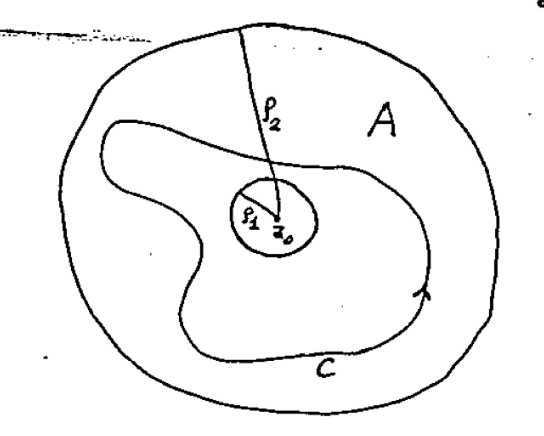
\includegraphics[width=0.45\textwidth]{images/p446.png}
\end{figure}

Si noti che, nel caso particolare in cui tutti i $c_n$ con $n$ negativi fossero nulli,
\begin{equation}
c_n = 0 \quad \text{per} \quad n = -1, -2, -3, \ldots, \tag{3}
\end{equation}
allora lo sviluppo di Laurent si ridurrebbe allo sviluppo di Taylor, e in realtà la $W(z)$ non sarebbe singolare in $z_0$. In tal caso, e solo in tal caso, i coefficienti $c_n$ con $n$ non negativi risulterebbero come sappiamo proporzionali alla stessa funzione $W(z)$ ed alle sue derivate, calcolate in $z_0$:
\begin{equation}
c_n = W^{(n)}(z_0) / n!\,, \quad n = 0, 1, 2, \ldots \tag{4}
\end{equation}

Per dimostrare i risultati testé enunciati, si utilizzi il teorema di Cauchy per scrivere
\[
\int_C dz'\; W(z') / (z' - z) = 0
\]
essendo la curva chiusa $C$ quella indicata nella seguente figura:

\begin{figure}[h]
\centering
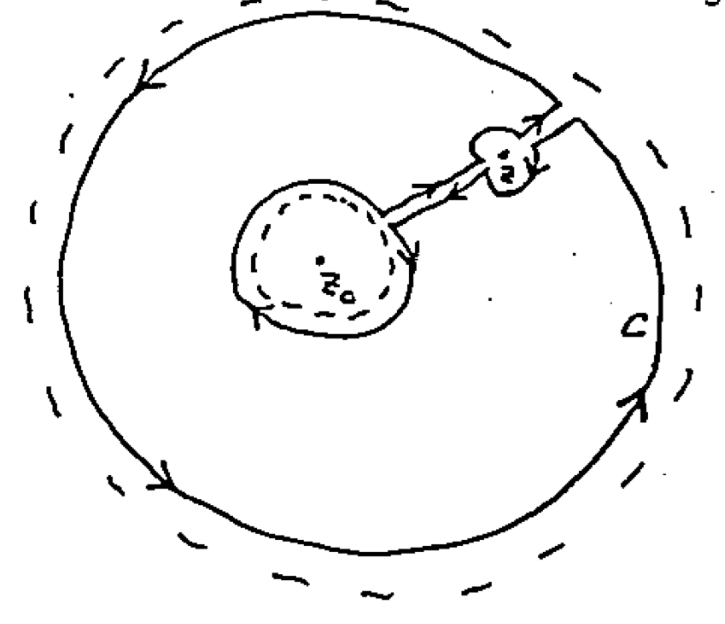
\includegraphics[width=0.45\textwidth]{images/p4462.png}
\end{figure}

% pagina 443 — 8.6-4
(si noti che questa curva è tutta racchiusa entro il dominio anulare e non contiene il punto $z$, sicché l'integrando è all'interno di $C$ privo di singolarità). Spezziamo ora la curva $C$ in 8 pezzi, come indicato in figura

\begin{figure}[h]
\centering
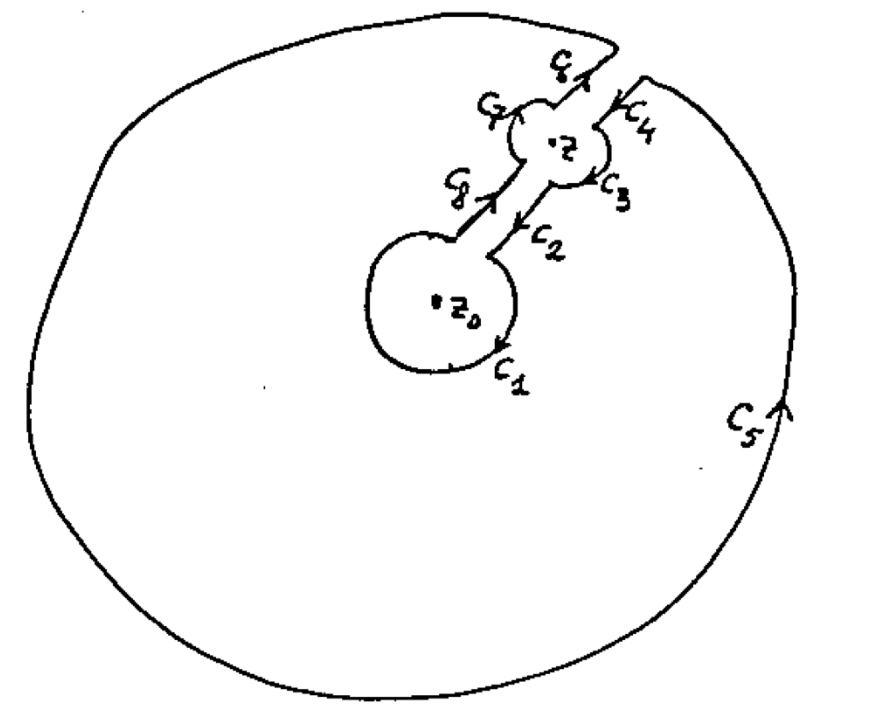
\includegraphics[width=0.45\textwidth]{images/p447.png}
\end{figure}

Sarà dunque
\[
\sum_{k=1}^{8} \int_{C_k} dz'\; w(z') / (z' - z) = 0.
\]
Supponiamo ora che i due segmenti di curva $C_2$ e $C_8$, nonché $C_4$ e $C_6$, siano infinitamente avvicinati l'uno all'altro; allora, \underline{come conseguenza della ipotesi di monodromia di $W(z)$}, sarà
\[
\int_{C_2} dz'\; w(z') / (z' - z) = -\int_{C_8} dz'\; w(z') / (z' - z)
\]
e analogamente per $C_4$ e $C_6$. Si ottiene così
\[
\int_{C_1} dz'\; w(z')/(z'-z) + \int_{C_5} dz'\; w(z')/(z'-z) = -\int_{C_3 + C_7} dz'\; w(z')/(z'-z).
\]
Ma, nel limite considerato, la curva $C_3 + C_7$ si chiude intorno a $z$ (ed è percorsa in senso orario), sicché l'integrale a secondo membro si riduce a $-W(z)$ (rappresentazione di Cauchy di $-W(z)$). Otteniamo così in conclusione
\[
W(z) = \int_{C''} dz''\; w(z'')/(z''-z) - \int_{C'} dz'\; w(z')/(z'-z)
\]
dove ora le due curve chiuse $C'$ e $C''$ sono due circonferenze (vedi figura nella pag. seguente).

È chiaro da questa discussione che la condizione cui debbono soddisfare queste circonferenze (centrate in $z_0$) affinché valga la formula testé ottenuta è
\[
\rho_1 < \rho' < \rho < \rho'' < \rho_2
\]
dove $\rho$ è la distanza del punto $z$ da $z_0$,
\[
\rho = |z - z_0|\,,
\]

% pagina 444 — 8.6-5
\begin{figure}[h]
\centering
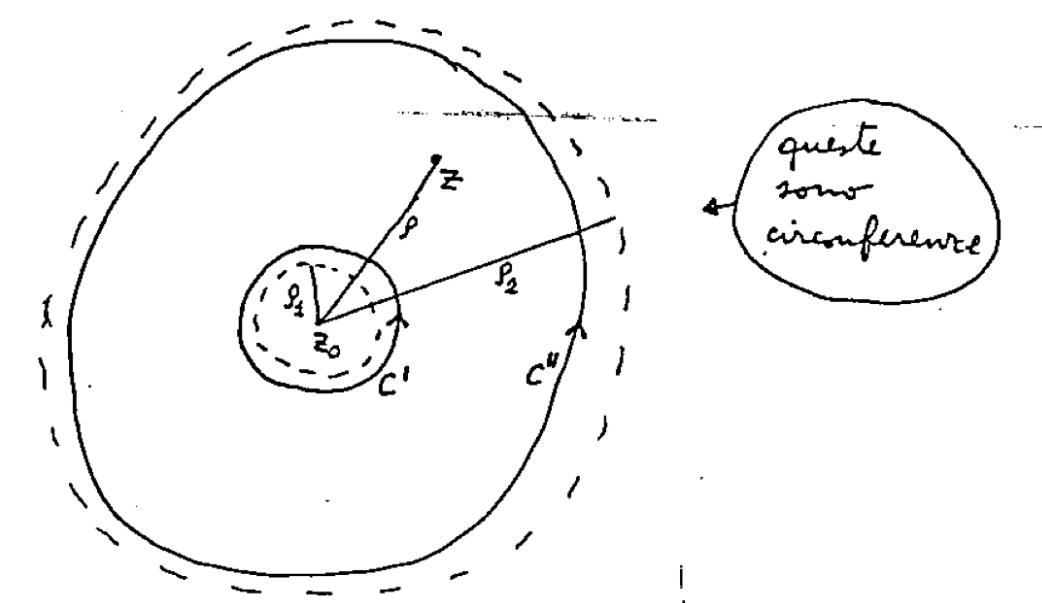
\includegraphics[width=0.45\textwidth]{images/p448.png}
\end{figure}

e i due raggi $\rho_1$ e $\rho_2$ sono i raggi minore e maggiore dell'anello $A$. È anche chiaro che $\rho_1$ può essere scelto arbitrariamente piccolo, e che $\rho_2$ dovrà essere maggiore di $\rho_1$ e minore della distanza $d$ da $z_0$ della (altra) singolarità di $W(z)$ che cade più vicina a $z_0$ stesso.

Si può ora procedere in modo analogo a quanto si era fatto nel caso dello sviluppo in serie di Taylor, osservando che si può scrivere
\[
(z''-z)^{-1} = \sum_{n=0}^{\infty} (z-z_0)^n \big/ (z''-z_0)^{n+1},
\]
risultando la serie a secondo membro assolutamente convergente (ed inoltre uniformemente convergente in $z''$) se $|z-z_0| < |z''-z_0|$, e viceversa
\[
(z'-z)^{-1} = -\sum_{n=0}^{\infty} (z'-z_0)^n \big/ (z-z_0)^{n+1},
\]
risultando la serie a secondo membro assolutamente convergente (ed inoltre uniformemente convergente in $z'$) se $|z-z_0| > |z'-z_0|$. Sostituendo dunque la prima formula nel primo integrale e la seconda nel secondo, otteniamo
\[
W(z) = \sum_{n=0}^{\infty} a_n\,(z-z_0)^n + \sum_{m=0}^{\infty} b_m \big/ (z-z_0)^{m+1}
\]
con
\[
a_n = \int_{C''} dz\; w(z) \big/ (z-z_0)^{n+1}
\]
\[
b_m = \int_{C'} dz\; w(z)\;(z-z_0)^m
\]
Ma l'espressione di $W(z)$ così ottenuta coincide proprio con la formula (1) dello sviluppo in serie di Laurent, poiché la (2) autorizza la identificazione
\[
c_n = a_n\,, \quad n = 0, 1, 2, 3, \ldots,
\]
\[
c_n = b_{-n-1}\,, \quad n = -1, -2, -3, \ldots
\]
Si noti infatti che il teorema di Cauchy autorizza ad eseguire la integrazione, nelle formule che definiscono i coefficienti $a_n$ e $b_n$, indifferen-%
% pagina 445 (senza numero sezione esplicito)
te sui contorni chiusi $C'$ o $C''$, o su un qualunque altro contorno $C$ (come nella (2)) che condivida con le curve $C'$ e $C''$ la proprietà di essere incluso in $A$, percorso in senso antiorario, e tale da circumnavigare una sola volta il punto $z_0$.

Si è così dimostrata la validità delle formule (1) e (2), nonché la assoluta convergenza dello sviluppo di Laurent (1) entro ogni dominio anulare concentrico a $z_0$, di raggio interno $\rho_1$ piccolo a piacere, e raggio esterno $\rho_2 = d$, essendo $d$ la distanza da $z_0$ della più vicina singolarità di $w(z)$.

Lo sviluppo in serie di Laurent converge dunque per anelli. Ma una volta definita una funzione analitica tramite il suo sviluppo in serie di Laurent nell'intorno del suo punto singolare $z_0$, è evidentemente possibile continuarla analiticamente anche al di fuori dell'anello, seguendo esattamente la stessa tecnica discussa nella sezione precedente (si noti che, nell'intorno di ogni punto $z$ interno all'anello, la $W(z)$ sarà ovviamente sviluppabile in serie di Taylor).

Lo sviluppo in serie di Laurent caratterizza il comportamento di una funzione analitica monodroma nell'intorno di una sua singolarità isolata. Esso può essere scomposto in due parti: la somma in cui compaiono esponenti negativi, cui si dà il nome di \underline{parte principale} dello sviluppo in serie di Laurent, e la somma in cui compaiono esponenti non negativi. Se la parte principale dello sviluppo di Laurent contiene una somma infinita, cioè $\forall N$ scelto $N$ grande quanto si vuole, vi sono sempre dei coefficienti $c_n$ con $n < -N$ diversi da zero, si dice che la funzione $W(z)$ ha in $z_0$ una \uline{singolarità essenziale}. Se invece la parte principale dello sviluppo di Laurent si arresta al termine di ordine $-N$, cioè
\begin{equation}
c_{-N} \neq 0, \quad c_n = 0 \;\text{ per }\; n < -N\,, \quad (N>0), \tag{5}
\end{equation}
allora si dice che, nel punto $z_0$, la $W(z)$ ha un \uline{polo di ordine $N$}. Una singolarità essenziale può dunque essere considerata un polo di ordine infinito.

Poli e singolarità essenziali sono dunque i due tipi di singolarità caratteristici delle funzioni analitiche monodrome.

Il comportamento di una funzione analitica nell'intorno di una singolarità essenziale è descritto dal seguente \underline{teorema di Weierstrass}, che riportiamo qui senza dimostrazione (anche se non sarebbe difficile darla): \uline{se la funzione analitica $W(z)$ ha una singolarità essenziale in $z_0$, scelti comunque il numero complesso $c$ ed i numeri reali positivi (piccoli a piacere) $\varepsilon$ e $\delta$, esiste sempre un punto $z$ che disti da $z_0$ meno di $\delta$ (per il quale cioè $|z - z_0| < \delta$)}%
% pagina 446 — 8.6-7
\uline{e tale che $W(z)$ differisca da $c$ meno di $\varepsilon$, sia cioè $|W(z) - c| < \varepsilon$}.

In parole povere il teorema di Weierstrass dice che, in un intorno per quanto piccolo del punto di singolarità essenziale $z_0$, la funzione $W(z)$ si avvicina quanto si vuole a qualunque numero complesso. Un perfezionamento del teorema di Weierstrass assicura anzi che, \uline{in un intorno arbitrariamente piccolo di un punto di singolarità essenziale, la funzione $w(z)$ assume tutti i valori complessi possibili, con l'eccezione, al più, di due numeri} (teorema di Picard).

Questi risultati implicano ovviamente che la funzione $w(z)$, nell'intorno di un suo punto di singolarità essenziale, non può mantenersi limitata, e che, se in $z_0$ $w(z)$ ha una singolarità essenziale, il limite di $w(z)$ per $z \to z_0$ non potrà essere univocamente definito, ma dovrà necessariamente dipendere dalla direzione, nel piano complesso, secondo cui $z$ si avvicina a $z_0$ (e in certe direzioni potrà anche non esistere affatto).

L'esempio tipico di funzione avente una singolarità essenziale nel punto $z_0$ è
\begin{equation}
W(z) = \exp\!\left[c/(z - z_0)\right]. \tag{6}
\end{equation}

Nell'intorno di un suo polo il comportamento di una funzione analitica è invece assai meno fantasioso; in effetti è ovvio dallo sviluppo di Laurent (che non vale naturalmente in $z = z_0$, ma vale però per $z$ arbitrariamente vicino a $z_0$) che, se $w(z)$ ha in $z_0$ un polo di ordine $N$ ($1 \leq N < \infty$), per $z \to z_0$ (in qualunque direzione) $w(z)$ diverge (cioè, scelto un numero reale positivo $M$ arbitrariamente grande, esisterà sempre un numero reale positivo $\delta$ tale che, per ogni $z$ che dista da $z_0$ meno di $\delta$, $|z - z_0| < \delta$, la funzione $w(z)$ supera $M$ in modulo, $|w(z)| > M$).

Esistono numerosi teoremi relativi al numero e alla posizione dei poli (e anche degli zeri, cioè i valori di $z$ per i quali $W(z) = 0$) di una funzione monodroma, per i quali si rinvia però alla letteratura.

Come vedremo, un ruolo particolarmente importante (tanto nel caso di singolarità essenziale, che di singolarità polare) viene assunto dal coefficiente $c_{-1}$ dello sviluppo di Laurent, cui si dà il nome di \underline{residuo}; nel seguito verrà generalmente indicato con la notazione
\begin{equation}
\mathrm{Res} \equiv c_{-1}\,. \tag{7}
\end{equation}
Vale infatti il seguente:

% pagina 447 — 8.6-8
\uline{Teorema dei residui}: \uline{l'integrale di una funzione analitica monodroma lungo una curva chiusa (percorsa in senso antiorario) è pari alla somma dei residui di tutte le singolarità (poli o singolarità essenziali) che cadono all'interno del contorno stesso}:
\begin{equation}
\int_C dz\; w(z) = 2\pi i \sum_k \mathrm{Res}_k\,. \tag{8}
\end{equation}

Si suppone naturalmente che la curva $C$ non incontri nessuna singolarità (altrimenti l'integrale non sarebbe neppure ben definito). Nello enunciare il teorema si è inoltre supposto che la curva $C$ sia connessa (e non si intersechi); si lascia al lettore la ovvia generalizzazione al caso in cui $C$ costituisce la frontiera di un dominio multiplamente connesso (si veda anche la dimostrazione data immediatamente sotto, e si ricordi la analoga situazione per il teorema di Cauchy).

La dimostrazione della (8) segue immediatamente dalla espressione dello sviluppo di Laurent (1) (con la notazione (7)), e dalla formula (vedi l'esercizio 3-3)
\begin{align}
\int_C dz\;(z-z_0)^n &= 0 \quad \text{se} \quad n = 0, 1, \pm 2, \pm 3, \pm 4, \ldots, \tag{9a}\\
&= 2\pi i \quad \text{se} \quad n = -1\,, \tag{9b}
\end{align}
valida per qualunque curva $C$ includente il punto $z_0$ (e percorsa in senso antiorario).

Si effettui infatti l'integrale di $w(z)$ lungo una qualunque curva $C_k$ che circondi la singolarità (polo o singolarità essenziale) che $w(z)$ ha in $z_k$, e lasci al di fuori tutte le altre singolarità. Sostituendo entro l'integrale la espressione (1) di $w(z)$ (cosa certo lecita se la curva $C_k$ è sufficientemente vicina a $z_k$, per la assoluta e uniforme convergenza dello sviluppo di Laurent) e usando le (9) si otterrà allora
\[
\int_{C_k} dz\; w(z) = 2\pi i\; \mathrm{Res}_k
\]
se con $\mathrm{Res}_k$ si indica il residuo di $w(z)$ in $z_k$. Considerando una opportuna curva $C_k$ per ogni singolarità $z_k$, si ottiene così
\[
\sum_k \int_{C_k} dz\; w(z) = 2\pi i \sum_k \mathrm{Res}_k\,.
\]
Ma è anche (vedi la eq.\ (3-7))
\[
\sum_k \int_{C_k} dz\; w(z) = \int_{\sum_k C_k} dz\; w(z)\,.
\]
Utilizzando ora la possibilità di deformare a piacere, grazie al teorema%
% pagina 448 — 8.6-9
di Cauchy, ciascuna delle curve $C_k$, purché senza urtare nessuna singolarità, ed usando il fatto che integrazioni lungo tratti comuni a due curve, se fatta in senso inverso, si elidono, si può fare in modo (vedi figura qui sotto) che
\[
\int_{\sum_k C_k} dz\; w(z) = \int_C dz\; w(z)
\]
essendo la curva $C$ percorsa in senso antiorario e includente tutte le singolarità distinte dall'indice $k$. Il teorema dei residui risulta così dimostrato.

\begin{figure}[h]
\centering
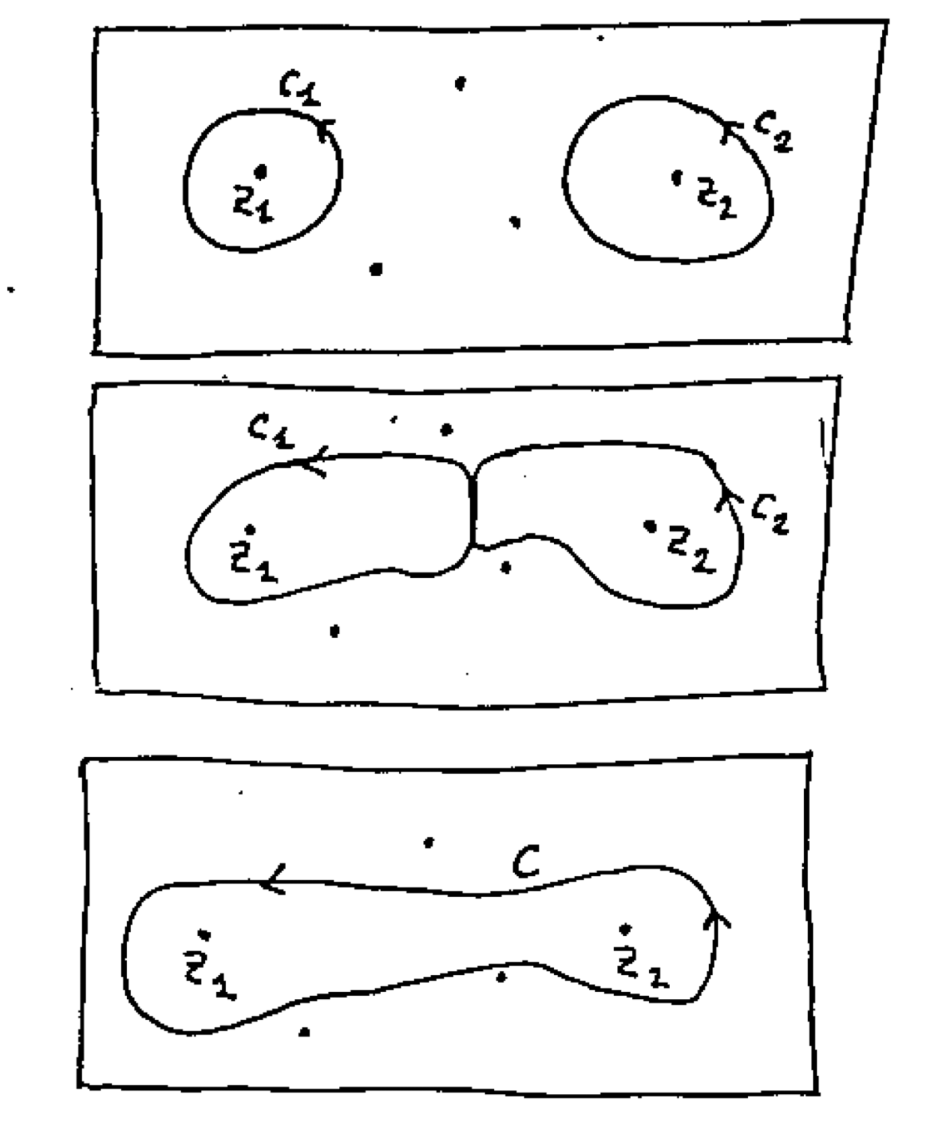
\includegraphics[width=0.7\textwidth]{images/p452.png}
\end{figure}

L'importanza del teorema dei residui sta nel fatto che è generalmente più facile effettuare il calcolo dei residui di una funzione analitica che non farne l'integrale. La (8) permette pertanto di valutare degli integrali nel campo complesso (e, come vedremo nella sezione seguente, anche nel campo reale), che sarebbero altrimenti difficili da effettuare.

Il calcolo del residuo di una funzione analitica $w(z)$ nel punto $z_0$ in cui ha un polo di ordine $N$ è facilitato dalla seguente formula:
\begin{equation}
\mathrm{Res} = \frac{1}{(N-1)!} \left\{ \frac{d^{N-1}}{dz^{N-1}} \left[ (z-z_0)^N W(z) \right] \right\}\Bigg|_{z=z_0} \tag{10}
\end{equation}
che segue immediatamente dallo sviluppo di Laurent.

Se la funzione $w(z)$ ha in $z_0$ un polo di ordine $N$, il suo sviluppo di Laurent nell'intorno di $z_0$ sarà
\[
W(z) = \sum_{n=-N}^{\infty} c_n\,(z-z_0)^n,
\]

% pagina 449 — 8.6-10
sicché
\[
(z-z_0)^N W(z) = \sum_{m=0}^{\infty} c_{m-N}\,(z-z_0)^m
\]
(avendo posto $m = n + N$). Differenziando $N-1$ volte, i primi $N-1$ termini della somma a secondo membro spariscono, e si ottiene
\[
\frac{d^{N-1}}{dz^{N-1}}\left[(z-z_0)^N W(z)\right] = \sum_{m=N-1}^{\infty} c_{m-N}\,(z-z_0)^{m-(N-1)}\frac{m!}{(m-N+1)!}\,.
\]
Ponendo ora $z = z_0$, di tutta la somma resta solo il primo termine (per $m = N-1$), fornendo
\[
\left.\frac{d^{N-1}}{dz^{N-1}}\left[(z-z_0)^N W(z)\right]\right|_{z=z_0} = (N-1)!\; c_{-1}\,,
\]
che è per l'appunto la (10). C.V.D.

Nel caso più frequente, in cui il polo è del primo ordine ($N=1$), si ha semplicemente
\begin{equation}
\mathrm{Res} = \lim_{z \to z_0}\left[(z-z_0)\,w(z)\right]. \tag{11}
\end{equation}

La discussione di questa sezione è stata limitata al caso di funzioni monodrome, e si è per semplicità fatta l'ipotesi che la monodromia valesse in tutto il piano complesso. È però chiaro che l'analisi effettuata ha validità locale; quel che conta è la monodromia nell'intorno di un punto singolare isolato (punto singolare che sarà allora necessariamente o una singolarità essenziale o un polo, ed in un intorno anulare del quale varrà lo sviluppo di Laurent). Nulla vieta che quella stessa funzione analitica abbia, in altre regioni del piano complesso, il comportamento, e le singolarità, caratteristiche delle funzioni polidrome (vedi più oltre).

Osserviamo infine che si sono finora discusse le proprietà di una funzione analitica per valori finiti della variabile $z$. Quanto al comportamento nel ``punto all'infinito'' del piano complesso, esso è dato dalla prescrizione di sostituire alla variabile $z$ la variabile
\[
Z = 1/z\,,
\]
e considerare poi le proprietà della funzione $w(z)$ in questione, pensandola come funzione di $Z$, nel punto ($\sigma$ nell'intorno del punto) $Z=0$. Tali proprietà sono allora attribuite alla $w(z)$ nel punto (o nell'intorno del punto) all'infinito. Si noti che con questa prescrizione il punto all'infinito nel%
% pagina 450 — 8.6-11
piano complesso è essenzialmente unico.

Per esempio si dirà dunque che ogni polinomio di grado $N$ ha all'infinito un polo di ordine $N$; in effetti il polinomio stesso può essere considerato come la parte principale dello sviluppo di Laurent nell'intorno del punto all'infinito, parte principale che coincide in questo caso con l'intera funzione. Si dirà anche che le funzioni $\exp(cz)$, $\sin(cz)$, $\cos(cz)$ hanno una singolarità essenziale all'infinito.

\begin{esercizi}
\item Sia la funzione $w(z)$ una funzione analitica monodroma in tutto il piano complesso, le cui singolarità sono dunque solo poli o singolarità essenziali. Si dimostri che i residui della funzione $w'(z)$ (la derivata di $w(z)$; ovviamente il teorema varrà anche per ogni successiva derivata) sono tutti nulli.

\item Si scriva lo sviluppo di Laurent delle seguenti funzioni nell'intorno del punto $z_0$ indicato in ciascun caso, precisando inoltre il raggio (esterno) $d$ dell'anello al cui interno lo sviluppo stesso converge (nel caso in cui lo sviluppo sia fatto intorno al punto all'infinito, $z_0 = \infty$, il raggio $D$ si riferisce alla variabile $1/z$):
\begin{enumerate}
\item[i)] $W(z) = \left[z(1-z)\right]^{-1}$, \quad $z_0 = 0$;
\item[ii)] $W(z) = \left[z(1-z)\right]^{-1}$, \quad $z_0 = 1$;
\item[iii)] $W(z) = \left[z(1-z)\right]^{-1}$, \quad $z_0 = \infty$;
\item[iv)] $W(z) = \left[z^2+1\right]^{-2}$, \quad $z_0 = i$;
\item[v)] $W(z) = \left[z^2+1\right]^{-2}$, \quad $z_0 = \infty$;
\item[vi)] $W(z) = z^2 \exp(c/z)$, \quad $z_0 = 0$.
\end{enumerate}
(Nota bene: può anche darsi, in qualche caso, che lo sviluppo di Laurent non contenga la parte principale, si riduca cioè ad uno sviluppo di Taylor).

\item Indicare quali delle seguenti funzioni possono essere sviluppate in serie di Laurent nell'intorno del punto $z_0$ indicato in ciascun caso, e quali no:
\begin{enumerate}
\item[i)] $W(z) = \sin(1/z)$, \quad $z_0 = 0$;
\item[ii)] $W(z) = \sin(1/z)$, \quad $z_0 = \infty$;
\item[iii)] $W(z) = 1/\sin z$, \quad $z_0 = 0$;
\item[iv)] $W(z) = 1/\sin z$, \quad $z_0 = \infty$;
\item[v)] $W(z) = 1/\cos(1/z)$, \quad $z_0 = 0$;
\item[vi)] $W(z) = z^2\,\mathrm{tg}(1/z)$, \quad $z_0 = 0$.
\end{enumerate}

% pagina 451 — 8.6-12
\item Si determinino i residui delle seguenti funzioni in tutti i punti in cui hanno singolarità (escluso il punto all'infinito):
\begin{enumerate}
\item[i)] $W(z) = 1/(z^3 - z^5)$;
\item[ii)] $W(z) = z^2/(z^2+1)^2$;
\item[iii)] $W(z) = z^{2n}/(1+z)^n$, \quad $n$ intero positivo;
\item[iv)] $W(z) = \mathrm{tg}\,z$;
\item[v)] $W(z) = z^n \sin(1/z)$, \quad $n$ intero.
\end{enumerate}

\item[*] La funzione $w(z)$ abbia i) un polo di ordine $N$ in $z_0$, ii) uno zero di ordine $N$ in $z_0$. Sia
\[
\nu(z) = w'(z)/w(z)\,.
\]
Si dimostri che la funzione $\nu(z)$ ha un polo semplice in $z_0$, con residuo $\pm N$ (il segno $+$ nel caso i), il segno $-$ nel caso ii)).

\item Si valutino i seguenti integrali nel piano complesso $z = x + iy$ eseguiti lungo le curve chiuse (percorse in senso antiorario) le cui equazioni sono indicate in ciascun caso:
\begin{enumerate}
\item[i)] $I = \int_C dz/(z^4+1)$, \quad $C:\; x^2+y^2-2x=0$;
\item[ii)] $I = \int_C dz\; z/[(z-1)(z-2)^2]$, \quad $C:\; |z-2|=1/2$;
\item[iii)] $I = \int_C dz\exp(z)/[z^2(z^2-9)]$, \quad $C:\; |z|=1$;
\item[iv)] $I = \int_C dz\;\sin(1/z)$, \quad $C:\; |z|=1$;
\item[v)] $I = \int_C dz\;\sin^2(1/z)$, \quad $C:\; |z|=1$;
\item[vi)] $I = \int_C dz\; z/[\sin z\,(1-\cos z)]$, \quad $C:\; |z|=5$;
\item[vii)] $I = \int_C dz\;(1+z+z^2)\left\{\exp(1/z) + \exp[1/(z-1)] + \exp[1/(z-2)]\right\}$, \quad $C:\; |z|=3$;
\item[viii)] $I = \int_C dz\; z^n \exp(2/z)$, \quad $n=0,\pm 1,\pm 2,\ldots$, \quad $C$ una qualunque curva includente l'origine.
\end{enumerate}

\item Si dimostri il seguente teorema: \uline{se $w(z)$ è una funzione monodroma in tutto il piano complesso ed ammette solo singolarità isolate, e se}
\[
\lim_{z \to \infty}\left[|z|\,w(z)\right] = 0
\]
\uline{(per $z \to \infty$ in ogni direzione nel piano complesso), allora la somma dei residui della funzione $w(z)$ in tutte le sue singolarità è nulla}.
Si osservi che un ovvio corollario di questo teorema è la formula (valida per funzioni $w(z)$ del tipo sopra considerato)
\[
\frac{1}{2\pi i}\int_C dz\; w(z) = \sum_k \mathrm{Res}_k = -\sum_{k'} \mathrm{Res}_{k'}
\]
essendo al solito la curva $C$ chiusa e percorsa in senso antiorario, estendendosi la somma sull'indice $k$ ai residui delle singolarità interne al cammino di integrazione (teorema dei residui) e la somma sull'indice $k'$%
% pagina 452 — 8.6-13/8.7-1
ai residui di tutte le singolarità \underline{esterne} al contorno di integrazione. In alcuni casi la seconda somma può essere più semplice da valutare della prima.

\item Si valuti l'integrale
\[
I = \int_C dz \Big/ \left[(z-3)(z^5-1)\right]
\]
esteso alla circonferenza $C$ di raggio 2 e centro in $z_0 = 0$. (Suggerimento: usare il corollario del teorema dell'esercizio precedente).
\end{esercizi}

\section{Calcolo di integrali mediante il teorema dei residui.}
% [sezione 8.7]

Come abbiamo visto nella precedente sezione, il teorema dei residui facilita grandemente il calcolo di integrali estesi a curve chiuse nel campo complesso (a condizione che l'integrando sia, entro il contorno, una funzione analitica monodroma con singolarità isolate).

Più importante per le applicazioni è la possibilità di effettuare integrali nel campo reale, trasformandoli in integrali su un contorno chiuso nel campo complesso. In questa sezione indichiamo come questo procedimento permetta di effettuare due tipi piuttosto generali di integrali definiti.

La prima classe di integrali è del tipo
\begin{equation}
I = \int_0^{2\pi} d\theta\; R(\cos\theta,\, \sin\theta) \tag{1}
\end{equation}
con $R(t_1, t_2)$ funzione \underline{razionale} dei due argomenti $t_1$ e $t_2$. Infatti ponendo
\begin{equation}
z = e^{i\theta} \tag{2}
\end{equation}
che implica
\begin{equation}
dz = i\,e^{i\theta}\,d\theta \tag{3a}
\end{equation}
ovvero
\begin{equation}
d\theta = -i\,dz/z \tag{3b}
\end{equation}
e, per le formule di Moivre,
\begin{equation}
\cos\theta = (z+z^{-1})/2\,, \quad \sin\theta = (z-z^{-1})/(2i)\,, \tag{4}
\end{equation}
si ottiene
\begin{equation}
I = -i \int_C dz\; w(z) \tag{5}
\end{equation}

% pagina 453 — 8.7-2
con
\begin{equation}
W(z) = z^{-1}\, R\!\left[(z+z^{-1})/2,\; (z-z^{-1})/(2i)\right]. \tag{6}
\end{equation}
La curva $C$ è il cerchio di raggio unitario e centro nell'origine, percorso in senso antiorario.

Ma questo integrale si può ora effettuare mediante il teorema dei residui, che fornisce
\begin{equation}
I = 2\pi \sum_k \mathrm{Res}_k \tag{7}
\end{equation}
essendo la somma a secondo membro estesa a tutti i residui della funzione $w(z)$, eq.\ (6), corrispondenti a singolarità che cadono, nel piano della variabile complessa, entro un cerchio di raggio unitario e centro nell'origine.

Nella ipotesi summenzionata, che la funzione $R(t_1, t_2)$ sia una funzione razionale dei suoi argomenti, anche $w(z)$ sarà una funzione razionale, cioè del tipo
\begin{equation}
w(z) = P_N(z) \big/ Q_M(z)\,, \tag{8}
\end{equation}
con $P_N(z)$, $Q_M(z)$ polinomi in $z$ di grado $N$ ed $M$ rispettivamente. In tal caso il teorema dei residui è certamente applicabile, essendo la funzione $w(z)$ ovviamente monodroma ed avendo solo singolarità isolate (anzi solo poli, che coincideranno con gli zeri del polinomio $Q_M(z)$).

Si noti però che questo procedimento si può applicare \underline{anche a casi in cui $R(t_1, t_2)$ non sia funzione razionale dei suoi argomenti}, salvo a verificare che la funzione $w(z)$, ottenuta da $R(t_1, t_2)$ mediante la (7), sia, nel cerchio centrato nell'origine e di raggio unitario, analitica monodroma salvo che per un numero (finito) di singolarità isolate.

Come esempio di applicazione delle precedenti considerazioni, si consideri l'integrale
\[
I = \int_0^{2\pi} d\theta\; \left\{\exp\!\left[a\,e^{i\theta}\right]\right\} \big/ \left[1 + b\cos\theta\right]
\]
con $a$ e $b$ costanti e $|b| < 1$. La prescrizione (7) fornisce allora
\[
W(z) = 2\exp(az) \big/ (bz^2 + 2z + b)\,.
\]
Le singolarità di $w(z)$ cadono dunque nei 2 punti
\[
z_{\pm} = \left(-1 \pm \sqrt{1-b^2}\right)\big/b\,.
\]
Poiché $z_+ z_- = 1$, e dunque anche $|z_+||z_-| = 1$, dei due numeri%
% pagina 454 — 8.7-3
complessi $z_+$ e $z_-$ uno sarà interno e l'altro esterno alla circonferenza di raggio unitario centrata nell'origine (i cui punti soddisfano ovviamente alla condizione $|z|=1$). È facile convincersi che il punto interno è $z_+$. Riscrivendo la funzione $w(z)$ nella forma
\[
W(z) = (2/b)\left[\exp(az)\right] \big/ \left[(z-z_-)(z-z_+)\right]
\]
si vede subito che il residuo di $W(z)$ in $z_+$ è
\[
\mathrm{Res} = (2/b)\left[\exp(az_+)\right] \big/ (z_+ - z_-)
\]
ovvero
\[
\mathrm{Res} = \exp\!\left\{(a/b)\left[(1-b^2)^{1/2}-1\right]\right\} \big/ \left[1-b^2\right]^{1/2}.
\]
Sicché in conclusione
\begin{align*}
\int_0^{2\pi} d\theta\; \left\{\exp\!\left[a\,e^{i\theta}\right]\right\} \big/ \left[1+b\cos\theta\right]
&= 2\pi\,(1-b^2)^{-1/2}\,\exp\!\left\{(a/b)\left[(1-b^2)^{1/2}-1\right]\right\}.
\end{align*}

Si osservi che il risultato è reale, se $a$ e $b$ sono reali ($e$ $|b|<1$); nel caso $a=0$ questo era prevedibile a priori, non così invece per $a \neq 0$.

Si osservi inoltre che la condizione $|b|<1$ (per $b$ reale) è necessaria affinché l'integrale risulti definito (non diverga).

Si osservi infine che, differenziando $n$ volte rispetto ad $a$, si ottiene la formula più generale
\begin{align*}
\int_0^{2\pi} d\theta\; \left\{\exp\!\left[a\,e^{i\theta}\right]\right\} &\exp(in\theta) \big/ \left[1+b\cos\theta\right] \\
&= 2\pi\,(1-b^2)^{-\frac{1}{2}} \left\{\left[(1-b^2)^{1/2}-1\right]/b\right\}^n \exp\!\left\{(a/b)\left[(1-b^2)^{1/2}-1\right]\right\},
\end{align*}
valida per $n$ intero (non negativo). È istruttivo — ed elementare — riottenere questa stessa formula applicando la tecnica di integrazione mediante estensione al campo complesso direttamente all'integrale a primo membro.

Una seconda importante classe di integrali che possono essere effettuati utilizzando il teorema dei residui è del tipo
\begin{equation}
I = \int_{-\infty}^{+\infty} dx\; f(x)\,. \tag{9}
\end{equation}

Si supponga infatti che la funzione $f(x)$ della variabile reale $x$ sia continuabile analiticamente; esista cioè una funzione analitica della variabile complessa $z$ che, per $z = x$, $x$ reale, coincida con la funzione $f(x)$. Come è naturale una tale funzione, se esiste, verrà indicata con la notazione%
% pagina 455 — 8.7-4
$f(z)$, ed al posto della (9) si potrà, in modo del tutto equivalente, scrivere
\begin{equation}
I = \int_C dz\; f(z)\,, \tag{10}
\end{equation}
coincidendo il cammino $C$ con l'intero asse reale, percorso da $-\infty$ a $+\infty$.

Si supponga ora che la funzione $f(z)$ goda della proprietà
\begin{equation}
\lim_{z \to \infty} \left[|z|^{1+\varepsilon}\,f(z)\right] = 0 \quad \text{per} \quad 0 \leq \arg z \leq \pi \tag{11}
\end{equation}
per valori di $\varepsilon$ positivi (ancorché piccoli).

La condizione (11), per $\arg(z)=0$ e $\arg(z)=\pi$, garantisce che l'originario integrale (9) sia convergente; la (11) è però assai più restrittiva, richiedendo \underline{l'annullarsi asintotico in ogni direzione nel semipiano superiore della variabile complessa $z$}.

Ebbene se la funzione $f(z)$, oltre a godere della proprietà (11), è monodroma nel semipiano superiore della variabile $z$ (cioè in tutta la zona del piano complesso in cui $z$ ha parte immaginaria non negativa) ed ha ivi solo singolarità isolate (poli o singolarità essenziali), è facile dimostrare che
\begin{equation}
I = 2\pi i \sum_k \mathrm{Res}_k \tag{12}
\end{equation}
essendo la somma a secondo membro estesa ai residui di tutte le singolarità di $f(z)$ localizzate nel semipiano complesso superiore (è forse il caso di sottolineare che si debbono considerare solo le singolarità al finito).

Per dimostrare il risultato testé enunciato, si consideri l'integrale di $f(z)$ esteso ad una curva chiusa formata da una parte dell'asse reale e da un semicerchio di raggio $R$ sufficientemente grande da far sì che tutte le singolarità di $f(z)$ siano incluse all'interno di tale contorno:

\begin{figure}[h]
\centering
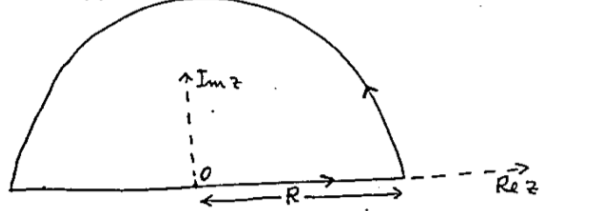
\includegraphics[width=0.5\textwidth]{images/fig_8-7-4.png}
\end{figure}

È chiaro che l'integrale esteso a tale circuito è, per il teorema dei residui, pari alla somma dei residui di tutte le singolarità di $f(z)$ che si trovano nel semipiano superiore della variabile $z$ (si noti che, come risulta dalla figura, il contorno è percorso in senso antiorario):
\[
\int_C dz\; f(z) = 2\pi i \sum_k \mathrm{Res}_k\,.
\]
Ma il contorno $C$ è composto dal tratto di asse reale da $-R$ ad $R$%
% pagina 456 — 8.7-5
e dal semicerchio $S_R$ di raggio $R$ nel semipiano superiore, sicché
\[
\int_C dz\; f(z) = \int_{-R}^{R} dx\; f(x) + \int_{S_R} dz\; f(z)\,.
\]
E la dimostrazione è completata osservando che, nel limite $R \to \infty$, il primo integrale coincide con l'integrale che si voleva calcolare,
\[
\lim_{R \to \infty} \left[\int_{-R}^{R} dx\; f(x)\right] = \int_{-\infty}^{+\infty} dx\; f(x)\,,
\]
laddove il secondo si annulla
\[
\lim_{R \to \infty} \left[\int_{S_R} dz\; f(z)\right] = 0\,.
\]
Infatti, parametrizzando tale semicerchio con la posizione
\[
z = R\,e^{i\theta}\,, \quad 0 \leq \theta \leq \pi\,,
\]
si ottiene
\[
\int_{S_R} dz\; f(z) = iR \int_0^{\pi} d\theta\; e^{i\theta}\, f\!\left[R\,e^{i\theta}\right].
\]
Da questa segue immediatamente
\[
\left|\int_{S_R} dz\; f(z)\right| \leq \pi\, M_R
\]
con
\[
M_R = \max_{0 \leq \theta \leq \pi} \left\{ R\, f\!\left[R\,e^{i\theta}\right] \right\}.
\]
E l'argomento è completato osservando che la (11) implica
\[
\lim_{R \to \infty} \left[M_R\right] = 0\,.
\]

In conclusione la possibilità di effettuare l'integrale definito dalla (9) discende dalla possibilità di continuare analiticamente l'integrando $f(x)$ in tutto il semipiano superiore, ottenendo una funzione analitica monodroma con singolarità isolate, e poi di chiudere il cammino di integrazione con un semicerchio di raggio grande (al limite, infinito) nel semipiano superiore, essendo il contributo dell'integrazione lungo tale semicerchio nullo (nel limite in cui il raggio del semicerchio tende all'infinito) grazie all'annullarsi asintotico della continuazione $f(z)$ della $f(x)$ in ogni direzione nel semipiano complesso superiore.

È chiaro d'altronde che, se la funzione $f(x)$ fosse continuabile analiticamente nel semipiano \underline{inferiore} anziché superiore, tale continuazione $f(z)$ fosse una funzione analitica monodroma con singolarità isolate, e%
% pagina 457 — 8.7-6
la $f(z)$ si annullasse per $z$ che diverge \underline{in ogni direzione nel semipiano inferiore} in modo che esista un $\varepsilon$ positivo, ancorché piccolo, tale che
\begin{equation}
\lim_{z \to \infty} \left[|z|^{1+\varepsilon}\,f(z)\right] = 0\,, \quad \pi \leq \arg z \leq 2\pi\,, \tag{13}
\end{equation}
allora
\begin{equation}
\int_{-\infty}^{+\infty} dx\; f(x) = -2\pi i \sum_k \mathrm{Res}_k\,, \tag{14}
\end{equation}
essendo ora la somma a secondo membro estesa ai residui di tutte le singolarità di $f(z)$ che cadono entro il semipiano inferiore della variabile complessa $z$, cioè tutte le singolarità che cadono in punti $z_k$ con $\mathrm{Im}\, z_k < 0$. Si noti il segno meno di fronte alla somma a secondo membro, dovuto al fatto che il circuito di integrazione ottenuto chiudendo il contorno con un semicerchio nel semipiano inferiore risulta percorso in senso orario.

In generale, nei casi in cui una tecnica di questo tipo possa essere usata, è il comportamento asintotico della $f(z)$ che prescrive se il contorno vada chiuso di sopra o di sotto; possono anche darsi casi in cui il comportamento asintotico della $f(z)$ è tale da permettere di chiudere sia sopra che sotto (ciò avviene se la $f(z)$ si annulla sufficientemente rapidamente — per $z \to \infty$ in qualunque direzione nel piano complesso); in tali casi le due scelte forniscono chiaramente lo stesso risultato (ma una può essere, da un punto di vista pratico, più conveniente dell'altra).

Un caso che si presenta spesso (anche in connessione con trasformate e antitrasformate di Fourier) è quello di integrali del tipo
\begin{equation}
I(\rho) = \int_{-\infty}^{+\infty} dx\; e^{i\rho x}\, f(x)\,, \tag{15}
\end{equation}
con $\rho$ parametro reale assegnato.

È allora chiaro che, se $f(x)$ è continuabile analiticamente e la continuazione $f(z)$ è monodroma, la tecnica precedente è applicabile, essendo la continuazione analitica dell'integrando la funzione
\begin{equation}
W(z) = e^{i\rho z}\, f(z)\,; \tag{16}
\end{equation}
e poiché, scrivendo $z = x + iy$, si vede che il fattore esponenziale
\begin{equation}
e^{i\rho z} = e^{i\rho x}\, e^{-\rho y}\,, \tag{17}
\end{equation}

% pagina 458 — 8.7-7
si annulla per $y \to +\infty$ e diverge per $y \to -\infty$ se $\rho > 0$ (e viceversa se $\rho < 0$), generalmente accade che il contorno vada chiuso di sopra per $\rho > 0$ e di sotto per $\rho < 0$.

Illustriamo quanto detto con un esempio, che ci permette inoltre di illustrare qualche artificio che risulta spesso assai utile per la valutazione di integrali nel campo complesso. Consideriamo l'integrale
\[
I(\rho) = \int_0^{\infty} dx\; \left(\frac{\sin(\rho x)}{x}\right)^2
\]
con $\rho$ parametro reale.

Un primo (banalissimo ma utilissimo) trucco si basa sulla osservazione che, essendo l'integrando una funzione pari, è possibile estendere l'integrale all'intero asse reale, scrivendo cioè
\[
I(\rho) = \frac{1}{2} \int_{-\infty}^{+\infty} dx\; \left(\frac{\sin(\rho x)}{x}\right)^2.
\]
È poi evidente che si può scrivere
\[
I(\rho) = \frac{1}{2} \int_C dz\; \left(\frac{\sin(\rho z)}{z}\right)^2
\]
essendo l'integrale sulla variabile complessa $z$ esteso ad un contorno $C$ che coincide con l'intero asse reale (percorso in senso positivo, cioè da sinistra a destra).

Poiché l'integrando è chiaramente finito in $z=0$ (ha il valore $\rho^2/2$), una modifica del cammino di integrazione quale quella indicata in figura cambierà in modo trascurabile il valore dell'integrale, se il raggio del piccolo semicerchio intorno all'origine è \underline{arbitrariamente piccolo}.

\begin{figure}[h]
\centering
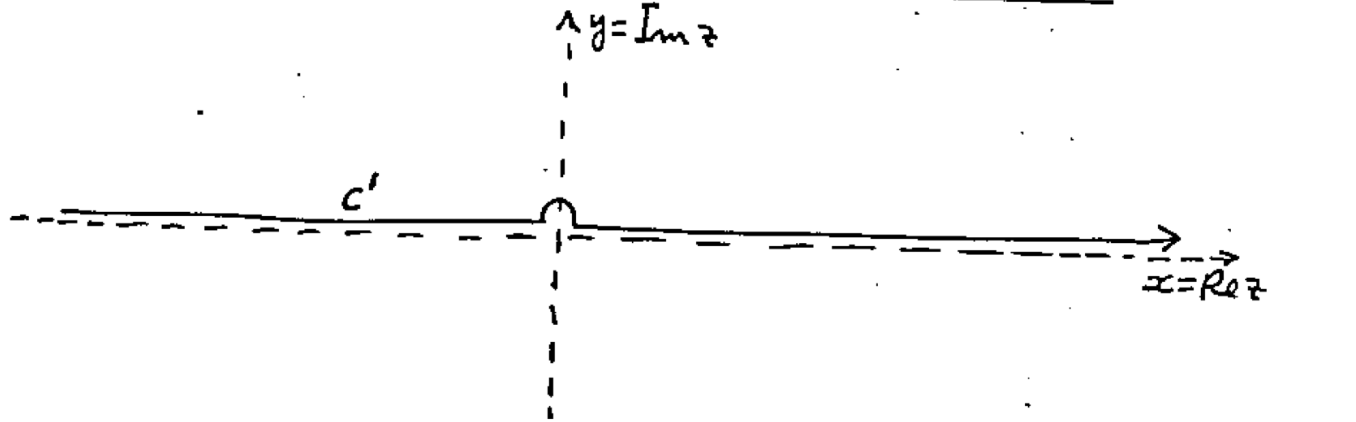
\includegraphics[width=0.6\textwidth]{images/fig_8-7-7.png}
\end{figure}

(Il cammino è stato disegnato un pochino spostato rispetto all'asse reale; ciò solo per esigenze grafiche, l'unica modificazione che si suppone sia stata introdotta è quella intorno all'origine).

Poiché il nuovo cammino evita di passare proprio per l'origine, possiamo ora esprimere il $\sin(\rho z)$ che compare nell'integrando tramite la formula di Moivre, eseguire il quadrato, scomponendo in tal modo l'integrale nella somma di tre integrali:
\begin{align*}
I(\rho) &= J_1(\rho) + J_2(\rho) + J_3(\rho)\,,\\
J_1(\rho) &= -\frac{1}{8} \int_{C'} dz\; \exp(2i\rho z) \big/ z^2\,,\\
J_2(\rho) &= -\frac{1}{8} \int_{C'} dz\; \exp(-2i\rho z) \big/ z^2\,,
\end{align*}

% pagina 459 — 8.7-8
\[
J_3(\rho) = \frac{1}{4} \int_{C'} dz \big/ z^2\,.
\]

Si noti che nessuno di questi integrali sarebbe separatamente definito se effettuato lungo l'originario cammino $C$; solo la loro somma $I(\rho)$ è costruita in modo che i diversi contributi, divergenti per $z=0$, si cancellino. La modifica del cammino di integrazione da $C$ a $C'$ è stata effettuata per permettere la definizione separata di questi tre integrali, il cui calcolo è, come vedremo, immediato.

Infatti, per il primo integrale, l'esponente è tale da permettere la chiusura del cammino con un grande semicerchio nel semipiano superiore se $\rho > 0$, inferiore se $\rho < 0$; si ottiene così
\begin{align*}
J_1(\rho) &= 0 \quad \text{se} \quad \rho > 0 \\
&= -\pi\rho/2 \quad \text{se} \quad \rho < 0
\end{align*}
(l'integrando ha una singolarità sola, in $z=0$, con residuo $-\frac{1}{2}i\rho$; nel primo caso tale singolarità resta però fuori dal cammino di integrazione, nel secondo viene aggirata in senso orario).

In modo analogo (ma chiudendo di sotto per $\rho > 0$, di sopra per $\rho < 0$) si ottiene
\begin{align*}
J_2(\rho) &= \pi\rho/2 \quad \text{se} \quad \rho > 0 \\
&= 0 \quad \text{se} \quad \rho < 0\,.
\end{align*}

Quanto a $J_3(\rho)$, esso può essere calcolato tanto chiudendo il cammino di sopra che di sotto; nel primo caso nessuna singolarità resta inclusa entro il contorno di integrazione, nel secondo caso la singolarità in $z=0$ è inclusa, ma l'integrando ha residuo nullo. In conclusione
\[
J_3(\rho) = 0\,.
\]

Combinando i risultati fin qui ottenuti si ha
\begin{align*}
I(\rho) &= \pi\rho/2 \quad \text{se} \quad \rho > 0 \\
&= -\pi\rho/2 \quad \text{se} \quad \rho < 0
\end{align*}
ovvero
\[
\int_{-\infty}^{+\infty} dx\; \left(\frac{\sin(\rho x)}{x}\right)^2 = \pi|\rho|/2\,, \quad (\rho \text{ reale}),
\]
che fornisce il risultato finale.

Si consiglia al lettore di verificare, eseguendo tutti i relativi passaggi, che lo stesso risultato si sarebbe ottenuto modificando l'iniziale cammino di integrazione in modo che esso aggiri il punto $z=0$ da sotto anziché da sopra.

Vi è una terza — assai meno generale — classe di integrali che possono essere anche ricondotti ad integrali su circuiti chiusi nel campo complesso, e dunque in ultima analisi ad una somma di residui. Si tratta di integrali del tipo
\begin{equation}
I = \int_0^{\infty} dx\; R(x^n)\,, \quad n = 2, 3, 4, 5, \ldots \tag{18}
\end{equation}

% pagina 460 — 8.7-9
con $R(t)$ funzione \underline{razionale} di $t$ e tale che
\begin{equation}
\lim_{t \to \infty} \left[R(t)\right] = 0\,. \tag{19}
\end{equation}
Si dimostra in tal caso che
\begin{equation}
I = -\left[\pi\,e^{-i\pi/n} \big/ \sin(\pi/n)\right] \sum_k \mathrm{Res}_k\,, \tag{20}
\end{equation}
essendo la somma a secondo membro estesa ai residui di tutte le singolarità della funzione
\begin{equation}
W(z) = R(z^n) \tag{21}
\end{equation}
che cadono entro il settore angolare del piano complesso $z$ caratterizzato dalla condizione
\begin{equation}
0 < \arg z < 2\pi/n\,. \tag{22}
\end{equation}
Si noti che a questo settore angolare del piano della variabile complessa $z$ corrisponde l'intero piano complesso per la variabile $t = z^n$.

Per dimostrare la (20), osserviamo anzitutto che l'ipotesi che $R(t)$ sia razionale — sia cioè il rapporto di due polinomi — implica che sia analiticamente continuabile, anzi che la funzione
\[
W(z) = R(z^n)
\]
sia analitica in tutto il piano complesso, salvo per un numero (finito) di poli.

Inoltre la (19), insieme alla condizione $n \geq 2$, implica non solo che l'integrale (18) è convergente, ma anche che
\[
\lim_{R \to \infty} \left[\int_{S_R} dz\; w(z)\right] = 0
\]
essendo $S_R$ un arco di cerchio di raggio $R$ nel piano complesso della variabile $z$. Infatti la (19), unita alla proprietà di $R(t)$ di essere una funzione razionale, implica che $R(t)$ si annulla almeno come $|t|^{-1}$ per $|t|$ grande; sicché se $t = z^n$ con $n = 2, 3, 4, \ldots$, $W(z)$ si annullerà almeno come $|z|^{-2}$ per $|z|$ grande. Ma noi abbiamo già visto che la condizione che $w(z)$ si annulli almeno come $|z|^{-1}$ per $|z| \to \infty$ è sufficiente per garantire l'annullarsi asintotico dell'integrale esteso ad un arco di cerchio di raggio divergente.

Osserviamo ora che la (18) si può anche scrivere
\[
I = \int_C dz\; w(z)
\]
con $w(z)$ fornito dalla (21), e coincidendo il cammino di integrazione $C$ con il semiasse reale positivo.

% pagina 461 — 8.7-10
Si introduce ora l'integrale
\[
I' = \int_{C'} dz\; w(z)
\]
essendo il cammino $C'$ costituito dalla semiretta uscente dall'origine e formante l'angolo $2\pi/n$ con l'asse reale positivo. Tale semiretta è dunque parametrizzata scrivendo
\[
z = \rho\,e^{2\pi i/n}
\]
con $\rho$ che varia da $0$ a $\infty$. Pertanto
\begin{align*}
I' &= \int_0^{\infty} d\rho\; e^{2\pi i/n}\, W\!\left[\rho\,e^{2\pi i/n}\right] \\
&= e^{2\pi i/n}\, I
\end{align*}
essendo il secondo passaggio giustificato dalla (18) unita alla osservazione secondo cui
\[
\left[\rho\,e^{2\pi i/n}\right]^n = \rho^n\,.
\]

D'altronde il teorema dei residui applicato al contorno chiuso costituito dal semiasse reale positivo, da un semiarco ``di raggio infinito'' e dalla semiretta formante l'angolo $2\pi/n$ con l'asse reale (percorsa in senso inverso, cioè dall'infinito fino all'origine) implica
\[
I - I' = \sum_k \mathrm{Res}_k\,.
\]
Sostituendo l'espressione di $I'$ in funzione di $I$ in questa equazione e risolvendo si ottiene così la (20), c.v.d.

È forse il caso di sottolineare che la tecnica testé introdotta fornisce dei risultati nuovi solo nel caso di $n$ dispari, in quanto per $n$ pari l'integrale (18) può essere effettuato con la tecnica discussa precedentemente (previa estensione dell'integrale da $-\infty$ a $+\infty$, cosa lecita — inserendo un fattore $1/2$ — in quanto per $n$ pari l'integrando è ovviamente pari).

Si ricordi inoltre che l'integrazione di funzioni razionali può sempre essere effettuata con tecniche dell'analisi elementare, anche se può risultare molto laboriosa; anzi tali tecniche permettono anche l'effettuazione di integrali indefiniti. Nel caso di integrali estesi ad intervalli infiniti (cui ci si può del resto sempre ricondurre, con opportuni cambiamenti di variabile) le tecniche di integrazione qui illustrate comportano generalmente calcoli meno lunghi.

In questa sezione abbiamo illustrato la possibilità di utilizzare%
% pagina 462 — 8.7-11
tecniche di continuazione analitica per effettuare integrali inizialmente definiti nel campo reale, e abbiamo sottolineato come ciò sia possibile a condizione che le funzioni ottenute per continuazione analitica siano monodrome (e con singolarità isolate). Come vedremo in una sezione successiva, tecniche analoghe possono essere impiegate per valutare integrali anche nel caso in cui ci si trovi ad aver a che fare con funzioni analitiche polidrome.

\begin{esercizi}
\item Si calcoli l'integrale
\[
I_{-n} = \int_0^{2\pi} d\theta\; \left\{\exp\!\left[a\,e^{i\theta}\right]\right\} \exp(-in\theta) \big/ \left[1 + b\cos\theta\right]
\]
con $a$ e $b$ costanti reali, $|b|<1$, ed $n$ intero positivo.

\item Si calcolino i seguenti integrali:
\begin{enumerate}
\item[i)] $I = \int_0^{2\pi} d\theta \big/ (a + b\cos\theta)^2$, \quad $a > b > 0$;
\item[ii)] $I = \int_0^{2\pi} d\theta \big/ (a + b\cos^2\theta)^2$, \quad $a > 0$, $b > 0$;
\item[iii)] $I = \int_0^{2\pi} d\theta \big/ (1 - 2c\cos\theta + c^2)$, \quad $c$ complesso, $|c| \neq 1$;
\item[iv)] $I = \int_0^{2\pi} d\theta\; \cos^2(3\theta) \big/ (1 - 2c\cos\theta + c^2)$, \quad $c$ complesso, $|c| \neq 1$;
\item[v)] $I_n = \int_0^{2\pi} d\theta\; \exp(\cos\theta)\,\cos(n\theta - \sin\theta)$, \quad $n$ intero;
\item[vi)] $I = \int_0^{\pi} d\theta\; \mathrm{tg}(x + ia)$, \quad $a$ reale, $a \neq 0$;
\item[vii)] $I = \int_0^{2\pi} d\theta\; \cot\mathrm{g}(x + ia)$, \quad $a$ reale, $a \neq 0$.
\end{enumerate}

\item Si calcolino gli integrali
\[
I_n(\rho) = \int_0^{\infty} dx\; \left(\frac{\sin(\rho x)}{x}\right)^n
\]
per $n=1, 3$ e $4$ ($\rho$ costante reale non nulla).

\item Si calcolino i seguenti integrali:
\begin{enumerate}
\item[i)] $I = \int_0^{\infty} dx \big/ (1+x^2)$;
\item[ii)] $I = \int_{-\infty}^{\infty} dx\; x \big/ (x^2+4x+13)^2$;
\item[iii)] $I = \int_0^{\infty} dx\; x^2 \big/ (x^2+a^2)^2$, \quad $a$ reale non nullo;
\item[iv)] $I = \int_{-\infty}^{+\infty} dx \big/ \left[(x^2+a^2)(x^2+b^2)\right]$, \quad $a$, $b$ reali non nulli;
\item[v)] $I = \int_0^{\infty} dx\; (x^2+1) \big/ (x^4+1)$.
\end{enumerate}

% pagina 463 — 8.7-12
\item Si calcolino gli integrali seguenti:
\begin{enumerate}
\item[i)] $I = \int_{-\infty}^{+\infty} \dfrac{dk}{2\pi}\; \dfrac{\exp(ikt)}{ik+\gamma}$, \quad $t$, $\gamma$ reali non nulli
\end{enumerate}
(si noti che questo integrale converge assolutamente; la condizione $t \neq 0$ è però essenziale per garantire la convergenza asintotica (non assoluta) mentre la condizione $\gamma \neq 0$ garantisce la convergenza in $k=0$);
\begin{enumerate}
\item[ii)] $I = \int_0^{\infty} dx\; \left[\cos(ax)\right] \big/ (x^2+b^2)$, \quad $a$, $b$ reali, $b \neq 0$;
\item[iii)] $I = \int_0^{\infty} dx\; \left[x\sin(ax)\right] \big/ (x^2+b^2)$, \quad $a$, $b$ reali;
\item[iv)] $I = \int_0^{\infty} dx\; \left[(x^2-b^2)\sin(ax)\right] \big/ \left[x(x^2+b^2)\right]$, \quad $a$, $b$ reali;
\item[v)] $I = \int_0^{\infty} dx\; \sin(ax) \big/ \left[x(x^2+b^2)\right]$, \quad $a$, $b$ reali, $b \neq 0$;
\item[vi)] $I = \int_0^{\infty} dx\; \sin(ax) \big/ \left[x(x^2+b^2)\right]$, \quad $a$, $b$ reali, $b \neq 0$; % [DUBBIO: v) e vi) sembrano identici nell'originale]
\item[vii)] $I = \int_0^{\infty} dx\; \left[\cos(2ax) - \cos(2bx)\right] \big/ x^2$, \quad $a$, $b$ reali.
\end{enumerate}

\item Si calcolino gli integrali seguenti:
\begin{enumerate}
\item[i)] $I_n = \int_0^{\infty} dx \big/ (1+x^n)$, \quad $n = 2, 3, 4, \ldots$;
\item[ii)] $J_n = \int_0^{\infty} dx\; x^n \big/ (1+x^{2n})$, \quad $n = 2, 3, 4, \ldots$
\end{enumerate}
\end{esercizi}

\section{Singolarità sul cammino di integrazione. Valor principale (alla Cauchy) di un integrale improprio.}
% [sezione 8.8]

Sinora abbiamo sempre supposto di avere a che fare con integrali estesi a cammini che evitano ogni punto singolare dell'integrando. Nelle applicazioni fisiche giocano però spesso un ruolo importante integrali estesi a cammini su cui l'integrando diventa singolare — integrali cui dovrà essere data una appropriata interpretazione, affinché essi assumano il corretto valore nell'ambito del problema fisico che li ha originati.

Un caso particolarmente importante è quello di integrali estesi a cammini sui quali l'integrando ha un polo semplice — ed è di questo caso che ci occuperemo in questa sezione.

Per fissare le idee, consideriamo dunque l'integrale
\[
\int_{-\infty}^{+\infty} dx\; f(x) \big/ (x - x_0)
\]
con $x_0$ reale ed $f(x_0) \neq 0$. Supponiamo inoltre che il comportamento di $f(x)$ per $x \to \pm\infty$ sia tale da escludere problemi di convergenza asintotica (è sufficiente che, per $\varepsilon$ positivo ancorché piccolo, $|x|^{\varepsilon} f(x) \to 0$ per $x \to \pm\infty$), e che la funzione analitica sia con-%
% pagina 464 — 8.8-2
tinuabile analiticamente, di modo che l'integrando sia la funzione analitica
\begin{equation}
W(z) = f(z) \big/ (z - x_0) \tag{1}
\end{equation}
avente un \underline{polo semplice} in $z = x_0$, con residuo $f(x_0)$.

L'integrale di questa funzione analitica su un cammino passante per il punto $x_0$ è chiaramente divergente. Si definisce invece \underline{valor principale} (alla Cauchy) di tale integrale il limite dell'integrale esteso ad un cammino ottenuto sottraendo da quello originario due tratti di uguale lunghezza $\varepsilon$ posti rispettivamente prima e dopo il punto $x_0$, e poi facendo il limite $\varepsilon \to 0$.

Per esempio in luogo dell'integrale scritto precedentemente (che, così come scritto, non aveva alcun senso matematico), si introduce l'integrale
\begin{equation}
P\!\int_{-\infty}^{+\infty} dx\; f(x)/(x-x_0) = \lim_{\varepsilon \to 0^+} \left\{\left[\int_{-\infty}^{x_0-\varepsilon} dx + \int_{x_0+\varepsilon}^{\infty} dx\right] f(x)/(x-x_0)\right\}. \tag{2}
\end{equation}

Come ora mostreremo, questo integrale ha un valore finito.

Si consideri infatti l'integrale esteso al cammino $C^{(+)}$ ottenuto modificando, con un semicerchio di raggio $\varepsilon$ e aggirante il punto singolare \underline{da sopra}, l'asse reale:

\begin{figure}[h]
\centering
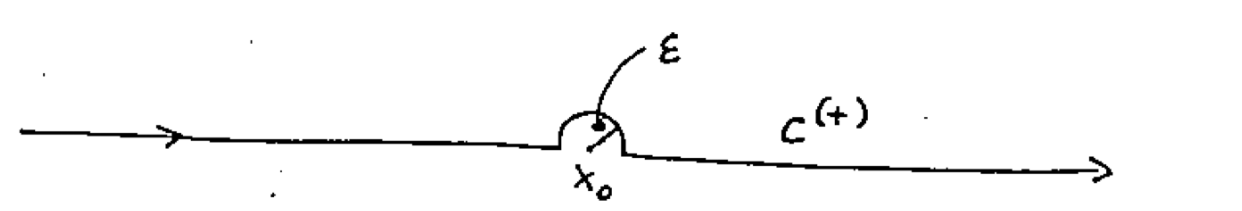
\includegraphics[width=0.5\textwidth]{images/fig_8-8-2.png}
\end{figure}

Chiaramente
\begin{equation}
\int_{C^{(+)}} dz\; W(z) = \int_{-\infty}^{x_0-\varepsilon} dx\; f(x)/(x-x_0) + \int_{x_0+\varepsilon}^{\infty} f(x)/(x-x_0) + \int_{C_\varepsilon} dz\; f(z)/(z-x_0)\,, \tag{3}
\end{equation}
ove con $C_\varepsilon$ si è indicato il semicerchio di raggio $\varepsilon$ nel semipiano superiore (percorso in senso orario).

È allora chiaro che, nel limite in cui $\varepsilon \to 0$,
\begin{equation}
\lim_{\varepsilon \to 0} \left[\int_{C^{(+)}} dz\; W(z)\right] = P\!\int_{-\infty}^{+\infty} dx\; f(x)/(x-x_0) - \pi i\, f(x_0)\,. \tag{4}
\end{equation}

Infatti poiché, sul cerchio $C_\varepsilon$, $z = x_0 + \varepsilon\,e^{i\theta}$, sarà
\[
\int_{C_\varepsilon} dz\; f(z)/(z-x_0) = i\int_{\pi}^{0} d\theta\; f\!\left[x_0 + \varepsilon\,e^{i\theta}\right]
\]

% pagina 465 — 8.8-3
sicché ovviamente
\[
\lim_{\varepsilon \to 0} \left[\int_{C_\varepsilon} dz\; f(z)/(z-x_0)\right] = -i\pi\, f(x_0)\,.
\]

Possiamo dunque concludere che
\begin{equation}
P\!\int_{-\infty}^{+\infty} dx\; f(x)/(x-x_0) = \pi i\, f(x_0) + \int_{C^{(+)}} dz\; f(z)/(z-x_0)\,, \tag{5}
\end{equation}
essendo il cammino $C^{(+)}$ coincidente con l'asse reale, ma tale da evitare il punto singolare aggirando\-lo da sopra. Naturalmente il cammino può essere poi modificato a piacere (in particolare, allontanato dal punto $x_0$), purché non si incontrino altre singolarità dell'integrando.

In modo del tutto analogo si sarebbe potuta ottenere la formula
\begin{equation}
P\!\int_{-\infty}^{+\infty} dx\; f(x)/(x-x_0) = -\pi i\, f(x_0) + \int_{C^{(-)}} dz\; f(z)/(z-x_0)\,, \tag{6}
\end{equation}
coincidendo ora il cammino $C^{(-)}$ con l'asse reale salvo la prescrizione di evitare il punto singolare passando \underline{da sotto}.

Un modo equivalente di scrivere questi stessi risultati è fornito dalla formula
\begin{equation}
\lim_{\varepsilon \to 0^+} \left[\int_{-\infty}^{+\infty} dx\; f(x) \big/ \left[x - (x_0 \pm i\varepsilon)\right]\right] = P\!\int_{-\infty}^{+\infty} dx\; f(x)/(x-x_0) \pm i\pi\, f(x_0)\,. \tag{7}
\end{equation}

L'equivalenza fra questa formula e le due precedenti deriva dalla possibilità di scrivere
\[
\int_{C^{(\pm)}} dz\; f(z)/(z-x_0) = \int_{-\infty}^{+\infty} dx\; f(x) \big/ \left[x - (x_0 \mp i\varepsilon)\right]\,,
\]
in quanto non è diverso (nel limite $\varepsilon \to 0$) modificare il cammino di integrazione per evitare la singolarità, o spostare la singolarità (dal punto $x_0$ al punto $x_0 \mp i\varepsilon$) per evitare che cada sull'asse reale. Naturalmente modificare il cammino aggirando la singolarità \underline{da sopra} è equivalente a spostare la singolarità \underline{sotto} al cammino di integrazione, lasciato immutato; e viceversa.

Spesso nella letteratura fisica la indicazione del limite è sottintesa, cioè ogni volta che si scrive un fattore $\left[x-(x_0 \pm i\varepsilon)\right]^{-1}$ si intende che esso vada valutato nel limite $\varepsilon \to 0^+$ (ma il limite va fatto dopo aver%
% pagina 466 — 8.8-4
integrato, non prima). La formula (7) si scrive anche, in forma stenografica (e con le consuete cautele di interpretazione associate all'uso della funzione delta di Dirac):
\begin{equation}
(x - x_0 \mp i\varepsilon)^{-1} = P\,(x-x_0)^{-1} \pm i\pi\,\delta(x-x_0)\,. \tag{8}
\end{equation}

Si noti che questa formula vale sia che si immagini di integrare su $x$ (per $x_0$ fisso), che anche se si supponesse di integrare su $x_0$ (per $x$ fisso).

Il valor principale di un integrale può naturalmente essere valutato, in certi casi, con il teorema dei residui; infatti le (5) e (6) lo mettono in diretta relazione con degli integrali (sui cammini $C^{(+)}$ e $C^{(-)}$) che possono essere valutati, in certi casi, con le tecniche della sezione precedente. Per esempio se la funzione $f(z)$ fosse priva di singolarità nel semipiano superiore e si annullasse (più rapidamente di $|z|^{-\varepsilon}$, con $\varepsilon$ arbitrariamente piccolo) per $z \to \infty$ in tale semipiano, dalla (5) (o anche dalla (6)) seguirebbe
\begin{equation}
P\!\int_{-\infty}^{+\infty} dx\; f(x)/(x-x_0) = \pi i\, f(x_0)\,, \tag{9}
\end{equation}
e viceversa si avrebbe
\begin{equation}
P\!\int_{-\infty}^{+\infty} dx\; f(x)/(x-x_0) = -\pi i\, f(x_0) \tag{10}
\end{equation}
se la funzione $f(x)$ fosse analitica (priva di singolarità) nel semipiano inferiore, e si annullasse per $z \to \infty$ in ogni direzione in tale semipiano.

Questi risultati seguono immediatamente dalla possibilità di chiudere il cammino di integrazione con un grande semicerchio di sopra o di sotto, semicerchio che non contribuisce all'integrale per l'annullarsi asintotico dell'integrando (nel limite in cui il raggio del semicerchio diverge). Una volta chiuso il cammino di integrazione, si può applicare il teorema dei residui che, nel caso particolare considerato, fornisce un risultato nullo (si riduce cioè al teorema di Cauchy).

È forse il caso di sottolineare che la prescrizione del \underline{valor principale} fornisce una definizione finita dell'integrale (improprio) effettuato su un cammino contenente singolarità, solo nel caso in cui la singolarità in questione sia un \underline{polo semplice}. La finitezza del risultato è dovuta alla cancellazione dei contributi divergenti, ma di segno opposto, derivanti dalle zone immediatamente precedenti e seguenti la singolarità, sul cammino di%

% pagina 467 — 8.8-5
integrazione.

È chiaro che, sebbene si sia fatto riferimento, nella discussione, ad un integrale esteso ad un intervallo infinito, e coincidente con l'intero asse reale, la definizione di valor principale di un integrale improprio si può dare in modo del tutto analogo per ogni integrale (esteso ad un contorno finito o infinito, reale o complesso), purché naturalmente si abbia a che fare con funzioni analitiche (o analiticamente continuabili), e la singolarità da ``curare'' sia un polo semplice (e cada entro il cammino di integrazione, esclusi gli estremi).

Nel caso di problemi fisici, si ha spesso a che fare con integrali del tipo di quelli considerati in questa sezione, e la prescrizione su come vada trattata la singolarità — come un valore principale, oppure spostandola sopra o sotto al contorno di integrazione — dipende generalmente dalle condizioni al contorno.

Un esempio molto istruttivo ed importante è quello del calcolo delle funzioni di Green di un operatore differenziale mediante la trasformata di Fourier. Per esempio si consideri l'operatore differenziale
\[
L_x = \frac{d^2}{dx^2} + \rho^2
\]
con $\rho$ costante reale (per convenzione positiva). Sia
\[
g(x,y) = g(x-y)
\]
la funzione di Green di questo operatore, sicché (ponendo $t = x-y$)
\[
L_t\, g(t) = \delta(t)\,.
\]
Passando alla trasformata di Fourier,
\[
g(t) = \int_{-\infty}^{+\infty} \frac{dk}{2\pi}\; e^{ikt}\,\hat{g}(k)\,,
\]
e usando la trasformata di Fourier della funzione delta di Dirac,
\[
\delta(t) = \int_{-\infty}^{+\infty} \frac{dk}{2\pi}\; e^{ikt}\,,
\]
si ottiene immediatamente
\[
(-k^2 + \rho^2)\,\hat{g}(k) = 1\,,
\]
donde
\[
g(t) = \int_{-\infty}^{+\infty} \frac{dk}{2\pi}\; e^{ikt} \big/ (-k^2+\rho^2)\,.
\]
Questa formula ha però solo un significato formale, essendo l'integrale a secondo membro a rigore divergente a causa dei due poli in $k = \pm\rho$.

% pagina 468 — 8.8-6
Occorre dunque aggiungere, a questo integrale, una prescrizione che specifichi come vada trattata ciascuna singolarità (aggirandola da sopra, da sotto, oppure trattandola come un valor principale); e i diversi risultati che si otterranno forniranno tutte le funzioni di Green, ma caratterizzate da diverse condizioni al contorno. Quanto alle funzioni che si possono ottenere facendo la differenza tra tali diverse funzioni di Green, è facile vedere che sarebbero sempre, come è logico, soluzioni della equazione omogenea
\[
L_t\,\psi(t) = 0\,.
\]

Per esempio la prescrizione di evitare ambedue le singolarità \underline{da sopra} (realizzabile con il cammino 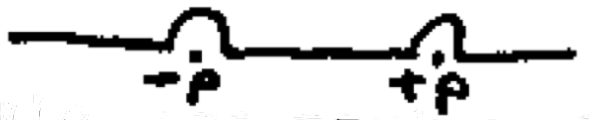
\includegraphics[height=1em]{images/cammino.png} % [DUBBIO: simbolo cammino nel testo]
nel piano complesso $k$; ovvero integrando lungo l'asse reale, ma scrivendo nel denominatore $\rho - i\varepsilon$ al posto di $\rho$, o equivalentemente $(-k^2 + \rho^2 - i\varepsilon)$ in luogo di $(-k^2+\rho^2)$) fornisce la funzione di Green \underline{ritardata}; si vede infatti subito, utilizzando il teorema dei residui, che tale funzione è nulla per $t > 0$ (per tali valori di $t$ è infatti possibile chiudere il cammino di integrazione con un grande semicerchio nel semipiano superiore). E viceversa evitando ambedue le singolarità \underline{da sotto} si ottiene la funzione di Green \underline{avanzata}. Anche importanti per le applicazioni sono la funzione di Green ``stazionaria'', che corrisponde alla scelta della prescrizione di ``valor principale'' per ambedue le singolarità, e la funzione di Green ``alla Feynman'' o ``causale'', che corrisponde ad evitare la singolarità in $-\rho$ da sotto e quella in $+\rho$ da sopra.

È forse il caso di sottolineare che, nel caso di problemi fisici, le diverse prescrizioni da usare per trattare ogni singolarità vanno decise caso per caso (in generale saranno determinate dalle condizioni al contorno). Si badi invece che, nella letteratura matematica — per esempio, nelle Tavoli di Integrali — la prescrizione che viene normalmente adottata, salvo esplicito contrario avviso, è quella di valor principale.

\begin{esercizi}
\item Si calcoli il valor principale dei seguenti integrali:
\begin{enumerate}
\item[i)] $I(t) = \int_{-\infty}^{+\infty} \dfrac{dk}{2\pi}\; e^{ikt} \big/ (k-\rho)$, \quad $\rho$ reale;
\item[ii)] $I = \int_0^1 dx \big/ (1-2x)$.
\end{enumerate}

\item Si calcolino esplicitamente le 4 funzioni di Green $g_a(t)$ (``avanzata''), $g_r(t)$ (``ritardata''), $g_{st}(t)$ (``stazionaria''), $g_c(t)$ (``causale''), dell'operatore differenziale
\[
L_x = \frac{d^2}{dx^2} + \rho^2\,, \quad \rho > 0\,, \quad t = x-y\,.
\]
Si verifichi esplicitamente che la differenza fra funzioni di Green diverse soddisfa l'equazione differenziale omogenea $L_t\,\psi(t) = 0$.
\end{esercizi}

\section[Funzioni analitiche polidrome e loro singolarità. Tagli e relative discontinuità; superficie di Riemann. Esempi]{Funzioni analitiche polidrome e loro singolarità (punti di diramazione). Tagli e relative discontinuità; superficie di Riemann. Esempi (logaritmo, potenza non intera).}
% [sezione 8.9]

In questa sezione discutiamo le funzioni analitiche polidrome e le loro singolarità.

Cominciamo la discussione considerando un esempio specifico, e precisamente la funzione definita dall'integrale
\begin{equation}
W(z) = \int_C dz' \big/ z' \tag{1}
\end{equation}
essendo la curva $C$ un cammino che parte dal punto $z_0 = 1$ e arriva al punto $z$, senza passare per il punto $z' = 0$. È facile dimostrare, usando il teorema di Cauchy, nonché il fatto che l'integrando nella (1) è analitico in tutto il piano complesso con la sola eccezione del punto $z'=0$ in cui ha un polo semplice con residuo pari ad 1, che il valore di $W(z)$ non dipende dal cammino $C$ (che va per ipotesi dal punto $z_0$ al punto $z$), salvo che per una particolare caratteristica; dipende cioè solo dal numero di volte che tale cammino gira intorno al punto $z'=0$. Anzi si trova precisamente che
\begin{equation}
W(z) = \mathrm{Log}\,z + 2\pi i\,n \tag{2}
\end{equation}
essendo per l'appunto $n$ il numero di volte che il cammino gira intorno a $z'=0$ in senso antiorario (un valore intero negativo di $n$ indicherebbe il numero di volte che il cammino gira intorno a $z'=0$ in senso orario — vedi figura), ed essendo per definizione $\mathrm{Log}(z)$ la \underline{determinazione principale} della funzione logaritmo,
\begin{equation}
\mathrm{Log}\,z = \log|z| + i\Theta\,, \quad 0 \leq \Theta < 2\pi\,. \tag{3}
\end{equation}
In questa formula naturalmente il numero reale positivo $|z|$ è il \underline{modulo} del numero complesso $z$, e il numero reale $\Theta$ è la \underline{fase} di $z$, caratterizzata dalla limitazione $0 \leq \Theta < 2\pi$:
\begin{equation}
z = |z|\,e^{i\Theta}\,, \quad |z|>0\,, \quad 0 \leq \Theta < 2\pi\,. \tag{4}
\end{equation}

% pagina 470 — 8.9-2
\begin{figure}[h]
\centering
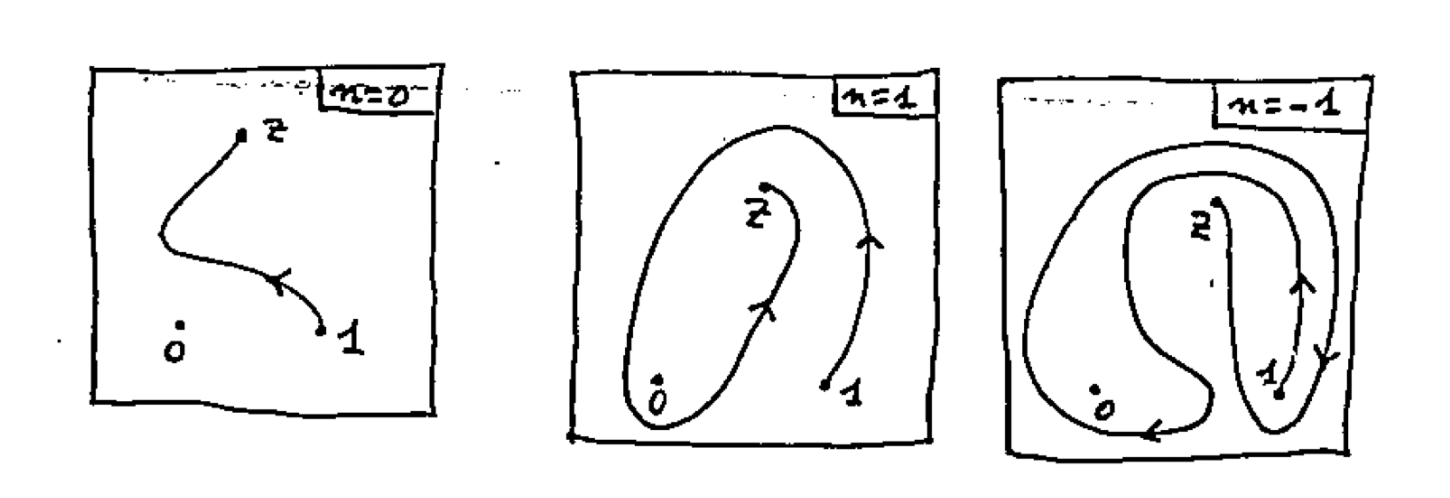
\includegraphics[width=0.7\textwidth]{images/fig_8-9-2.png}
\end{figure}

La formula (2) suggerisce di definire
\begin{equation}
\int_1^z dz' \big/ z' = \mathrm{Log}\,z\,. \tag{5}
\end{equation}
Si introduce così la funzione \underline{polidroma} $\log z$ (``logaritmo di $z$'' — naturalmente in base $e$), che assume, in ogni punto del piano complesso, gli infiniti valori
\begin{equation}
\log z = \mathrm{Log}\,z + 2\pi i\,n \tag{4}
\end{equation}
con $n$ intero.

È chiaro che questa ambiguità si può far corrispondere al fatto che la fase di un numero complesso è definita mod$(2\pi)$, cioè se $z = |z|\,e^{i\Theta}$ è un numero complesso, $z = |z|\,e^{i(\Theta + 2\pi n)}$ è lo stesso numero complesso (se $n$ è intero, positivo o negativo).

La funzione $\log(z)$ è dunque una funzione polidroma a infiniti valori. Tale polidromia è associata all'esistenza della singolarità in $z=0$, avente la caratteristica che, se si seguono con continuità (per esempio, con la tecnica di continuazione analitica alla Weierstrass) i valori di $\log(z)$ a partire da un punto $z_1$ lungo un cammino chiuso che ritorna a $z_1$, si riottiene o no lo stesso valore a seconda che il contorno abbia o no aggirato il punto $z=0$.

Singolarità di questa natura sono dette \underline{punti di diramazione}; si parlerà di punto di diramazione di ordine $n$ se, compiendo $n+1$ giri (nello stesso verso) intorno ad esso, la funzione torna ad assumere il valore iniziale (vedi esempi successivi); si parlerà di punto di diramazione%
% pagina 471 — 8.9-3
di ordine infinito se, per quante volte si giri attorno al punto singolare, la funzione non torna mai ad assumere lo stesso valore. Poiché, nel caso della funzione logaritmo, ogni giro (in senso antiorario) aggiunge la costante $2\pi i$, possiamo concludere che tale funzione ha, in $z=0$, un punto di diramazione di ordine infinito.

Ricordando che le proprietà di analiticità nel punto all'infinito corrispondono, per definizione, alle proprietà di analiticità in $Z=0$, con $Z=1/z$, si conclude inoltre che la funzione $\log(z)$ ha un punto di diramazione anche all'infinito. In effetti è una caratteristica generale dei punti di diramazione di apparire sempre a coppie.

A parte i due punti di diramazione in $z=0$ e $z=\infty$, la funzione $\log(z)$ è analitica. Ciò implica per esempio la convergenza dello sviluppo di Taylor
\begin{equation}
\log z = \log z_0 + \sum_{n=1}^{\infty} \left[(z-z_0)/z_0\right]^n \big/ n \tag{5}
\end{equation}
entro un cerchio di centro $z_0$ e raggio $|z_0|$, ovvero dello sviluppo (di Taylor in $Z - Z_0 = 1/z - 1/z_0$)
\begin{equation}
\log z = \log z_0 - \sum_{n=1}^{\infty} (-1)^n \left[(z-z_0)/z\right]^n \big/ n \tag{6}
\end{equation}
al di fuori dello stesso cerchio.

Il più semplice esempio di funzione avente un punto di diramazione di ordine finito (anzi del primo ordine) è fornito dalla funzione ``radice quadrata'':
\begin{equation}
W(z) = z^{1/2}\,. \tag{7}
\end{equation}

È infatti chiaro che, partendo convenzionalmente da $W(z) = +\sqrt{z}$ per $z$ reale positivo, $z=\rho$, otteniamo per $z = \rho\,e^{i\pi} = -\rho$ il valore immaginario positivo $W(z) = \sqrt{\rho}\,e^{i\pi/2} = i\sqrt{\rho}$, per $z = \rho\,e^{2\pi i} = \rho$ (cioè dopo un giro) il valore reale negativo $W(z) = \sqrt{\rho}\,e^{i\pi} = -\sqrt{\rho}$, per $z = \rho\,e^{3\pi i}$ il valore immaginario negativo $W(z) = \sqrt{\rho}\,e^{3\pi i/2} = -i\sqrt{\rho}$, e infine per $z = \rho\,e^{4\pi i}$ (cioè dopo avere fatto due giri intorno all'origine) di nuovo il valore $W(z) = \sqrt{\rho}\,e^{2\pi i} = +\sqrt{\rho}$.

% pagina 472 — 8.9-4
E con il solito sistema — passando cioè alla variabile $Z = 1/z$ — si può vedere che la funzione $W(z) = z^{1/2}$ ha un altro punto di diramazione del primo ordine nel punto all'infinito.

Si noti che, come è chiaro da questi esempi, in un punto di diramazione una funzione analitica può avere un valore ben definito e finito (per esempio, $W(z) = z^{1/2}$ in $z=0$ si annulla); non può però avere definite e finite tutte le derivate (altrimenti si potrebbe scrivere lo sviluppo di Taylor, e questo, convergendo in un cerchio, per quanto piccolo, fornirebbe una definizione univoca della funzione analitica in una zona che circonda il punto singolare, in contrasto con la definizione stessa di punto di diramazione). In questo senso un punto di diramazione è diverso da un polo o da un punto di singolarità essenziale, nei quali come sappiamo la funzione diverge (polo) o non è definita in modo non ambiguo (singolarità essenziale).

I valori di una funzione polidroma risultano definiti in modo univoco se, con qualche prescrizione, si proibisce di girare intorno ai punti di diramazione. Il modo più semplice di ottenere ciò, per una funzione avente due punti di diramazione, è di ``tagliare'' il piano complesso lungo una curva chiusa che va dall'uno all'altro punto di diramazione. Per esempio, per la funzione $\log(z)$, possiamo convenzionalmente stabilire di tagliare il piano complesso della variabile $z$ lungo l'asse reale positivo, da $z=0$ a $z=\infty$. Una volta assegnato il valore di $\log z$ in un qualunque punto $z$ del piano così tagliato (assegnato naturalmente non in modo arbitrario, ma solo nel senso di eliminare l'ambiguità inerente alla natura polidroma della funzione), ogni altro valore della funzione $\log(z)$ risulta, nel piano tagliato, univocamente definito (e ottenibile per esempio per continuazione analitica, alla Weierstrass). Se il valore assegnato fosse in un punto sull'asse reale, andrebbe ulteriormente specificato se tale valore va inteso assegnato sul bordo superiore, o inferiore, del taglio. Ed è evidente che, per i valori subito al di sopra e subito al disotto del taglio si ha la formula
\begin{equation}
\log\!\left[\rho\,e^{i\Theta}\right] - \log\!\left\{\rho\,e^{[(2\pi-\varepsilon)i]}\right\} = 2\pi i \tag{8}
\end{equation}
valida nel limite (sottinteso) $\varepsilon \to 0$.

Questa formula esprime la \underline{discontinuità} della funzione $\log(z)$ sul \underline{taglio}, che convenzionalmente è stato tirato da $z=0$ a $z=\infty$ lungo l'asse reale posi-%
% pagina 473 — 8.9-5
tivo.

In modo analogo considerando la funzione $W(z) = z^{1/2}$ e supponendo di tirare il taglio lungo l'asse reale negativo, da $z=0$ a $z=-\infty$, si otterrebbe per la discontinuità sul taglio la formula
\begin{equation}
\left\{\rho\,e^{i(\pi-\varepsilon)}\right\}^{1/2} - \left\{\rho\,e^{i(-\pi+\varepsilon)}\right\}^{1/2} = 2i\,\rho^{1/2}\,. \tag{9}
\end{equation}

Il fatto di aver definito, nel caso del logaritmo, il taglio lungo l'asse reale positivo, e nel caso della radice, lungo l'asse reale negativo, corrisponde alla convenzione di uso corrente; ma nulla vieterebbe di usare una diversa convenzione. Si noti inoltre che la formula (9) si riferisce alla discontinuità che si ha per quella determinazione della radice quadrata di $z$ che risulta, nel piano tagliato, univocamente definita dalla prescrizione di fornire valori reali positivi in corrispondenza a valori reali positivi della variabile $z$.

È dunque chiaro che, nel piano tagliato, si torna ad avere — per ogni determinazione della funzione analitica in questione — una funzione monodroma; per la quale varranno tutti i risultati discussi nelle precedenti sezioni. Si avranno però tante diverse funzioni — ciascuna monodroma — quante sono le possibili determinazioni della funzione polidroma di partenza (ovvero $n+1$, se $n$ è l'ordine dei due punti di diramazione connessi dal taglio). Per esempio, nel caso della funzione $\log(z)$, si avrà una infinità numerabile di funzioni monodrome, differenti l'una dall'altra per una costante additiva, in modo tale cioè che la loro differenza sia in ogni punto pari a $2\pi i\,\mathcal{V}$, con $\mathcal{V}$ intero. Nel caso della funzione radice quadrata, si avranno invece due funzioni, uguali ed opposte (cioè ottenibili l'una dall'altra mediante moltiplicazione per la costante $e^{i\pi} = -1$).

Una geniale idea di Riemann ha associato, ad ogni funzione analitica polidroma, anziché tante funzioni monodrome — le diverse determinazioni — definite in uno stesso piano complesso tagliato, una sola funzione, definita però su una superficie a più fogli in modo che, ad ogni valore della variabile $z$ su un certo foglio, corrisponda in modo univoco un valore della funzione. Tale superficie a più fogli sovrapposti è ottenuta supponendo che l'attraversamento di un taglio dia accesso ad un nuovo foglio della superficie, diverso da quello di provenienza. Nel caso, per esempio, del logaritmo, si avrà dunque una superficie di Riemann ad infiniti fogli, costruita in modo%
% pagina 474 — 8.9-6
che si passi da un foglio all'altro attraversando l'asse reale positivo; su ogni foglio di tale superficie di Riemann la funzione ha un valore unico, ed i valori assunti dalla funzione in corrispondenza a due uguali valori di $z$ situati però su due fogli diversi differiscono di $2\pi i\,\nu$, con $\nu$ intero ($\nu = \pm 1$ se i due fogli sono contigui; col segno $+$ o $-$ a seconda di come viene fatta la differenza). Nel caso della radice quadrata, la superficie di Riemann è composta da due fogli solamente, disposti in modo che il punto $z = \rho\,e^{i\pi}$ sul primo foglio coincida col punto $z = \rho\,e^{-i\pi}$ sul secondo foglio (e in questo punto $z^{1/2} = +i\sqrt{\rho}$), mentre il punto $z = \rho\,e^{-i\pi}$ sul primo foglio coincide col punto $z = \rho\,e^{+i\pi}$ sul secondo foglio (ed ivi $z^{1/2} = -i\,\rho^{1/2}$).

Ad ogni funzione analitica polidroma risulta così associata una \underline{superficie di Riemann} a più fogli, che può anche essere topologicamente assai complicata (una funzione analitica può avere tanti punti di diramazione); su tale superficie risulteranno localizzate le ulteriori singolarità della funzione, ed in particolare i poli e le singolarità essenziali (che potranno essere presenti su tutti i fogli o solo su alcuni).

Il principale merito della idea di Riemann è che, avendo introdotta la superficie di Riemann, ad ogni punto della quale risulta associato uno ed un solo valore della funzione analitica (salvo nel caso di poli o singolarità essenziali), è possibile applicare anche alle funzioni polidrome tutti i risultati precedentemente discussi per le funzioni monodrome. In particolare sono validi tutti i risultati connessi al teorema di Cauchy e al teorema dei residui, tenendo però conto che i cammini di integrazione passano, attraverso i tagli, da un foglio della superficie di Riemann all'altro (sicché un contorno risulta chiuso solo se, partendo da un punto su un dato foglio della superficie di Riemann, ritornando — magari attraversando più tagli, un numero pari di volte — ritorna allo stesso punto \underline{sullo stesso foglio} della superficie di Riemann). Di questo fatto si può approfittare, per esempio, per valutare degli integrali, in modo analogo a quanto fatto, nel caso di funzioni monodrome, nella sezione 7.

Altro pregio — non pratico, ma concettuale — della introduzione della superficie di Riemann associata ad ogni funzione analitica polidroma è lo stabilirsi di una stretta connessione fra due branche della matematica apparentemente assai lontane, quali la topologia e la teoria delle funzioni di variabile complessa; è infatti evidente che vi è uno stretto legame fra la%
% pagina 475 — 8.9-7
struttura topologica della superficie di Riemann e la struttura analitica della corrispondente funzione polidroma.

La discussione di questa sezione è stata largamente basata su due esempi, le funzioni $\log(z)$ e $z^{1/2}$, di cui si è dettagliatamente illustrata la struttura analitica, nonché la topologia delle corrispondenti superfici di Riemann. Terminiamo la sezione illustrando in qualche dettaglio altri due esempi.

Il primo esempio è quello della funzione
\begin{equation}
z^c = \exp\!\left[c\,\log z\right], \tag{10}
\end{equation}
con $c$ costante complessa arbitraria. È chiaro che la superficie di Riemann di questa funzione è analoga a quella della funzione $\log z$ (salvo nel caso in cui $c$ è un numero reale razionale; vedi sotto); ha cioè infiniti fogli, connessi l'uno all'altro tramite un taglio che, seguendo la convenzione corrente, può essere tirato lungo l'asse reale negativo, da $z=0$ a $z=-\infty$. Convenzionalmente sul foglio di Riemann che corrisponde alla determinazione principale della funzione si scriverà
\begin{align}
z^c &= |z|^c\,e^{ic\Theta} \tag{11a}\\
&= \exp\!\left\{c\left[\log|z| + i\Theta\right]\right\} \tag{11b}
\end{align}
essendo $\log(z)$ un numero reale (positivo o negativo a seconda che $|z|$ sia maggiore o minore di 1) ed essendo la fase $\Theta$ compresa fra $-\pi$ e $+\pi$; i valori di $z^c$ per $z = \rho\,e^{i\pi}$ e quelli per $z = \rho\,e^{-i\pi}$ sul foglio corrispondente a tale determinazione principale sono quelli sul labbro superiore e inferiore del taglio, e sono rispettivamente $\rho^c\,e^{ic\pi}$ e $\rho^c\,e^{-ic\pi}$; sicché la discontinuità sul taglio nel foglio corrispondente alla determinazione principale della funzione $z^c$ vale
\begin{equation}
\rho^c\!\left[\exp(ic\pi) - \exp(-ic\pi)\right] = 2i\,\rho^c\,\sin(c\pi)\,. \tag{12}
\end{equation}

Si noti che condizione necessaria e sufficiente affinché tale discontinuità sparisca è che $c$ sia un numero intero, nel qual caso non si ha più punto di diramazione né in $z=0$ né in $z=\infty$ e la funzione diventa monodroma.

Il punto $z = \rho\,e^{i\pi}$, in cui $z^c = \rho^c\,e^{ic\pi}$,%
% pagina 476 — 8.9-8
può essere considerato come localizzato sul bordo superiore del taglio nel foglio di Riemann corrispondente alla determinazione principale della funzione $z^c$; oppure può essere considerato come localizzato sul bordo inferiore del taglio sul foglio adiacente (in quanto attraverso il taglio si passa appunto al foglio adiacente); in tal caso si dovrebbe più logicamente denotare tale punto come $z = \rho\,e^{-i\pi}$, ma il valore della funzione $z^c$ in tale punto resterebbe lo stesso, $z^c = \rho^c\,e^{+ic\pi}$.

Insomma una volta introdotto il concetto di superficie di Riemann occorre ricordare che la funzione in questione può essere considerata monodroma, nel senso che in ogni punto della superficie di Riemann essa assume un ben determinato valore; ma per specificare un punto della superficie di Riemann non basta assegnarne le coordinate (cartesiane o polari) nel piano complesso, occorre anche specificare su quale foglio sta (è come per localizzare una particolare stanza di un palazzo; non basta darne le coordinate sulla pianta, ma occorre anche dire a che piano sta — salvo nel caso di un edificio ad un solo piano, che corrisponde, in questa analogia, al caso di una funzione monodroma).

È chiaro che, se si continua a girare, in senso antiorario, intorno al punto $z=0$, si passa a nuovi fogli della superficie di Riemann della funzione $z^c$; i valori della funzione $z^c$ che si ottengono dopo ogni giro sono pari a quelli sul foglio precedente moltiplicati per il fattore $e^{2\pi ic}$, sicché quelli che si ottengono dopo $n$ giri a partire dal foglio della determinazione principale sono pari a quelli della determinazione principale moltiplicati per il fattore $e^{2\pi icn}$. È chiaro che, se $c$ non è un numero razionale, il numero $cn$ non è mai intero (per $n$ intero), dunque il fattore $e^{2\pi icn}$ è sempre diverso da $1$ (per ogni $n$ intero), dunque i valori di $z^c$ nella stessa posizione ma su diversi fogli non coincidono mai. In questo caso la funzione polidroma $z^c$ ha infiniti valori, e la corrispondente superficie di Riemann ha infiniti fogli. Se invece $c$ fosse un numero intero razionale, $c = M/N$ con $M$ ed $N$ interi, allora per $n=N$
\begin{equation}
e^{2\pi icn} = e^{2\pi iM} = 1\,, \tag{13}
\end{equation}
sicché dopo $N$ giri la funzione torna ad assumere i valori iniziali. In questo caso la funzione polidroma $z^c = z^{M/N}$ ha $N$ valori, e la superficie di Riemann di tale funzione ha $N$ fogli; dal taglio sul foglio $(N-1)$-esimo%

si entra nel foglio $N$-esimo, ma dal taglio sul foglio $N$-esimo si entra nel
primo foglio. In questo caso i punti di diramazione, in $z=0$ e $z=\infty$, sono
di ordine $N-1$; nel caso precedente ($c$ complesso, oppure $c$ reale ma
non razionale) i punti di diramazione sono di ordine infinito (come quelli
della funzione $\log(z)$).

L'ultimo esempio che vogliamo discutere è quello della funzione
\begin{equation}
    W(z) = \left[(z-a)(z-b)\right]^{1/2} \,.
    \tag{14}
\end{equation}

Questa funzione ha 2 punti di diramazione del primo ordine in $z=a$ e $z=b$.

\medskip
\noindent
È facile verificare che $\left[(z-a)(z-b)\right]^{1/2}$ non ha punti
di diramazione, ma invece un polo semplice, all'infinito. Infatti ponendo
$Z = 1/z$ e $\tilde{W}(Z) = W(z) = \left[(z-a)(z-b)\right]^{1/2}$
si ha
\[
    \tilde{W}(Z) = \left[(1-aZ)(1-bZ)\right]^{1/2} / Z \,.
\]
Si noti che la radice è analitica nell'intorno di $Z=0$; è per esempio sviluppabile
in serie di potenze di $Z$ (serie di Taylor), risultando tale serie convergente
entro il cerchio centrato in $Z=0$ e di raggio pari al più piccolo dei due
numeri $|a|^{-1}$ e $|b|^{-1}$.

Dividendo tale serie di Taylor per $Z$ si ottiene la serie di Laurent di
$W(Z)$ nell'intorno di $Z=0$, che convergerà entro l'anello che si ottiene dal
cerchio sopra descritto eliminando un dischetto centrato in $Z=0$ e di raggio
arbitrariamente piccolo ancorché finito.

\medskip
\noindent
La funzione $W(z)$, eq.~(14), è dunque una funzione (polidroma) a due
valori; la sua superficie di Riemann ha 2 fogli. Essa può essere ottenuta
tracciando il taglio con una curva (per esempio un segmento) dal punto
$z=a$ al punto $z=b$ nel piano della variabile complessa $z$; oppure tracciando
il taglio lungo una curva che va da $a$ a $b$ passando per il punto all'infinito,
una curva cioè composta da due tratti che vanno rispettivamente da $a$ all'infinito
e da $b$ all'infinito (si ricordi che, nella topologia del piano complesso,
il punto all'infinito è unico).

Poiché una discussione a parole occuperebbe troppo spazio (e forse
non risulterebbe nemmeno chiara), ci limitiamo qui ad indicare, mediante
dei diagrammi, i valori che la funzione assume nei diversi casi. Ci riferiamo
per semplicità al caso $a=-1$, $b=+1$, sicché la funzione in discussione
è

% --- pagina 478 ---

\begin{align}
    W(z) &= \left[(z+1)(z-1)\right]^{1/2} \tag{15a}\\
         &= \left(z^2-1\right)^{1/2} \,. \tag{15b}
\end{align}

In ogni caso indichiamo nella figura i valori che tale funzione assume nei
punti $z=2$, $z=0$, $z=-2$; nel caso in cui tali punti cadano sul taglio, risulta
dalla figura stessa quale è il valore sopra e quale sotto.

Nel primo caso (taglio da $z=-1$ a $z=1$ passando per $z=0$): sul primo
foglio si ha

\begin{center}
\begin{tikzpicture}
  \node[draw, minimum width=9cm, minimum height=2.2cm, anchor=north west] (box) at (0,0) {};
  \node[anchor=north] at (4.5,0) {\small Valori di $(z^2-1)^{1/2}$ sul primo foglio};
  % taglio
  \draw[thick] (2.5,-1.1) -- (6.5,-1.1);
  % valori
  \node at (1.0,-0.7) {$-\sqrt{3}$};  \node[circle,fill,inner sep=1pt] at (1.3,-0.9){};
  \node at (4.5,-0.7) {$+i$};          \node[circle,fill,inner sep=1pt] at (4.5,-0.85){};
  \node at (4.5,-1.35) {$-i$};         \node[circle,fill,inner sep=1pt] at (4.5,-1.15){};
  \node at (7.8,-0.7) {$+\sqrt{3}$};   \node[circle,fill,inner sep=1pt] at (7.5,-0.9){};
\end{tikzpicture}
\end{center}

e sul secondo foglio

\begin{center}
\begin{tikzpicture}
  \node[draw, minimum width=9cm, minimum height=2.2cm, anchor=north west] (box) at (0,0) {};
  \node[anchor=north] at (4.5,0) {\small Valori di $(z^2-1)^{1/2}$ sul secondo foglio};
  \draw[thick] (2.5,-1.1) -- (6.5,-1.1);
  \node at (1.0,-0.7) {$+\sqrt{3}$};   \node[circle,fill,inner sep=1pt] at (1.3,-0.9){};
  \node at (4.5,-0.7) {$-i$};           \node[circle,fill,inner sep=1pt] at (4.5,-0.85){};
  \node at (4.5,-1.35) {$+i$};          \node[circle,fill,inner sep=1pt] at (4.5,-1.15){};
  \node at (7.8,-0.7) {$-\sqrt{3}$};    \node[circle,fill,inner sep=1pt] at (7.5,-0.9){};
\end{tikzpicture}
\end{center}

Nel secondo caso (taglio da $z=+1$ e $z=-1$ passando per il punto all'infinito):
sul primo foglio si ha:

\begin{center}
\begin{tikzpicture}
  \node[draw, minimum width=10cm, minimum height=2.5cm, anchor=north west] (box) at (0,0) {};
  \node[anchor=north] at (5,0) {\small Valori di $(z^2-1)^{1/2}$ sul primo foglio};
  % due semirette che escono dal box a sinistra e a destra
  \draw[thick] (0,-0.9) -- (2.0,-0.9);   % taglio sinistro
  \draw[thick] (8.0,-0.9) -- (10,-0.9);  % taglio destro
  \node at (1.0,-0.6) {$-\sqrt{3}$};     \node[circle,fill,inner sep=1pt] at (1.3,-0.85){};
  \node at (5.0,-0.6) {$i$};              \node[circle,fill,inner sep=1pt] at (5.0,-0.75){};
  % sopra/sotto il taglio destro
  \node at (8.5,-0.5) {$+\sqrt{3}$};     \node[circle,fill,inner sep=1pt] at (8.3,-0.75){};
  \node at (8.5,-1.2) {$-\sqrt{3}$};     \node[circle,fill,inner sep=1pt] at (8.3,-1.0){};
  \node at (1.3,-1.15) {$+\sqrt{3}$};
\end{tikzpicture}
\end{center}

e sul secondo foglio

\begin{center}
\begin{tikzpicture}
  \node[draw, minimum width=10cm, minimum height=2.5cm, anchor=north west] (box) at (0,0) {};
  \node[anchor=north] at (5,0) {\small Valori di $(z^2-1)^{1/2}$ sul secondo foglio};
  \draw[thick] (0,-0.9) -- (2.0,-0.9);
  \draw[thick] (8.0,-0.9) -- (10,-0.9);
  \node at (1.0,-0.6) {$+\sqrt{3}$};   \node[circle,fill,inner sep=1pt] at (1.3,-0.85){};
  \node at (5.0,-0.6) {$-i$};           \node[circle,fill,inner sep=1pt] at (5.0,-0.75){};
  \node at (8.5,-0.5) {$-\sqrt{3}$};   \node[circle,fill,inner sep=1pt] at (8.3,-0.75){};
  \node at (8.5,-1.2) {$+\sqrt{3}$};   \node[circle,fill,inner sep=1pt] at (8.3,-1.0){};
  \node at (1.3,-1.15) {$-\sqrt{3}$};
\end{tikzpicture}
\end{center}

% --- pagina 479 ---

Naturalmente la distinzione fra ``primo'' e ``secondo'' foglio è del tutto convenzionale.

\medskip
Per giustificare i risultati precedenti, si considerino separatamente le due funzioni
$W_1(z) = (z+1)^{1/2}$ e $W_2(z) = (z-1)^{1/2}$, e si costruisca per ciascuna
di loro un diagramma analogo a quelli indicati sopra, tenendo conto della
possibilità di tracciare, per la funzione $z^{1/2}$, il taglio lungo l'asse
reale positivo o negativo. Si hanno così, per la funzione $W_1(z) = (z+1)^{1/2}$,
due possibilità, alla prima delle quali corrispondono i due diagrammi

\begin{center}
\begin{tikzpicture}
  \node[draw, minimum width=8cm, minimum height=2cm, anchor=north west] (box) at (0,0) {};
  \node[anchor=north] at (4,0) {\small Valori di $(z+1)^{1/2}$ sul primo foglio};
  \draw[thick] (0,-0.9) -- (2.5,-0.9);
  \node at (3.5,-0.6) {$1$};   \node[circle,fill,inner sep=1pt] at (3.5,-0.8){};
  \node at (7.0,-0.6) {$\sqrt{3}$}; \node[circle,fill,inner sep=1pt] at (6.8,-0.8){};
  \node at (1.0,-0.5) {$i$};
  \node at (1.0,-1.1) {$-i$};
\end{tikzpicture}
\end{center}

\begin{center}
\begin{tikzpicture}
  \node[draw, minimum width=8cm, minimum height=2cm, anchor=north west] (box) at (0,0) {};
  \node[anchor=north] at (4,0) {\small Valori di $(z-1)^{1/2}$ sul secondo foglio};
  \draw[thick] (0,-0.9) -- (2.5,-0.9);
  \node at (3.5,-0.6) {$-i$};  \node[circle,fill,inner sep=1pt] at (3.5,-0.8){};
  \node at (3.5,-1.1) {$i$};
  \node at (7.0,-0.6) {$-\sqrt{3}$}; \node[circle,fill,inner sep=1pt] at (6.8,-0.8){};
  \node at (0.5,-0.6) {$-i$};
  \node at (0.5,-1.1) {$i$};
\end{tikzpicture}
\end{center}

e alla seconda delle quali corrispondono i due diagrammi

\begin{center}
\begin{tikzpicture}
  \node[draw, minimum width=8cm, minimum height=2.2cm, anchor=north west] (box) at (0,0) {};
  \node[anchor=north] at (4,0) {\small Valori di $(z+1)^{1/2}$ sul primo foglio};
  \draw[thick] (2.5,-0.9) -- (8,-0.9);
  \node at (3.5,-0.55) {$+1$};   \node[circle,fill,inner sep=1pt] at (3.5,-0.8){};
  \node at (3.5,-1.15) {$-1$};
  \node at (7.0,-0.55) {$+\sqrt{3}$}; \node[circle,fill,inner sep=1pt] at (6.8,-0.8){};
  \node at (7.0,-1.15) {$-\sqrt{3}$};
  \node at (1.0,-0.6) {$i$}; \node[circle,fill,inner sep=1pt] at (1.0,-0.8){};
\end{tikzpicture}
\end{center}

\begin{center}
\begin{tikzpicture}
  \node[draw, minimum width=8cm, minimum height=2.2cm, anchor=north west] (box) at (0,0) {};
  \node[anchor=north] at (4,0) {\small Valori di $(z-1)^{1/2}$ sul secondo foglio};
  \draw[thick] (2.5,-0.9) -- (8,-0.9);
  \node at (3.5,-0.55) {$-1$};  \node[circle,fill,inner sep=1pt] at (3.5,-0.8){};
  \node at (3.5,-1.15) {$+1$};
  \node at (7.0,-0.55) {$-\sqrt{3}$}; \node[circle,fill,inner sep=1pt] at (6.8,-0.8){};
  \node at (7.0,-1.15) {$+\sqrt{3}$};
  \node at (1.0,-0.6) {$-i$}; \node[circle,fill,inner sep=1pt] at (1.0,-0.8){};
\end{tikzpicture}
\end{center}

Analogamente per $W_2(z) = (z-1)^{1/2}$ si ha:

\begin{center}
\begin{tikzpicture}
  \node[draw, minimum width=8cm, minimum height=2.2cm, anchor=north west] (box) at (0,0) {};
  \node[anchor=north] at (4,0) {\small Valori di $(z-1)^{1/2}$ sul primo foglio};
  \draw[thick] (0,-0.9) -- (3.5,-0.9);
  \node at (0.7,-0.55) {$+i\sqrt{3}$}; \node[circle,fill,inner sep=1pt] at (0.9,-0.8){};
  \node at (0.7,-1.15) {$-i\sqrt{3}$};
  \node at (3.5,-0.55) {$+i$};         \node[circle,fill,inner sep=1pt] at (3.5,-0.8){};
  \node at (3.5,-1.15) {$-i$};
  \node at (7.0,-0.7) {$1$};           \node[circle,fill,inner sep=1pt] at (7.0,-0.85){};
\end{tikzpicture}
\end{center}

% --- pagina 480 ---

\begin{center}
\begin{tikzpicture}
  \node[draw, minimum width=8cm, minimum height=2.2cm, anchor=north west] (box) at (0,0) {};
  \node[anchor=north] at (4,0) {\small Valori di $(z-1)^{1/2}$ sul secondo foglio};
  \draw[thick] (0,-0.9) -- (3.5,-0.9);
  \node at (0.7,-0.55) {$-i\sqrt{3}$}; \node[circle,fill,inner sep=1pt] at (0.9,-0.8){};
  \node at (0.7,-1.15) {$+i\sqrt{3}$};
  \node at (3.5,-0.55) {$-i$};          \node[circle,fill,inner sep=1pt] at (3.5,-0.8){};
  \node at (3.5,-1.15) {$+i$};
  \node at (7.0,-0.7) {$-1$};           \node[circle,fill,inner sep=1pt] at (7.0,-0.85){};
\end{tikzpicture}
\end{center}

oppure

\begin{center}
\begin{tikzpicture}
  \node[draw, minimum width=8cm, minimum height=2.2cm, anchor=north west] (box) at (0,0) {};
  \node[anchor=north] at (4,0) {\small Valori di $(z-1)^{1/2}$ sul primo foglio};
  \draw[thick] (3.5,-0.9) -- (8,-0.9);
  \node at (0.7,-0.7) {$i\sqrt{3}$};  \node[circle,fill,inner sep=1pt] at (0.9,-0.85){};
  \node at (3.5,-0.55) {$i$};          \node[circle,fill,inner sep=1pt] at (3.5,-0.8){};
  \node at (7.0,-0.55) {$+1$};         \node[circle,fill,inner sep=1pt] at (7.0,-0.8){};
  \node at (7.0,-1.15) {$-1$};
\end{tikzpicture}
\end{center}

\begin{center}
\begin{tikzpicture}
  \node[draw, minimum width=8cm, minimum height=2.2cm, anchor=north west] (box) at (0,0) {};
  \node[anchor=north] at (4,0) {\small Valori di $(z-1)^{1/2}$ sul secondo foglio};
  \draw[thick] (3.5,-0.9) -- (8,-0.9);
  \node at (0.7,-0.7) {$-i\sqrt{3}$}; \node[circle,fill,inner sep=1pt] at (0.9,-0.85){};
  \node at (3.5,-0.55) {$-i$};         \node[circle,fill,inner sep=1pt] at (3.5,-0.8){};
  \node at (7.0,-0.55) {$-1$};         \node[circle,fill,inner sep=1pt] at (7.0,-0.8){};
  \node at (7.0,-1.15) {$+1$};
\end{tikzpicture}
\end{center}

La struttura della superficie di Riemann, nonché i valori, della funzione
$W(z) = \left[(z+1)(z-1)\right]^{1/2}$ si ottengono da quelli di $W_1(z)=(z+1)^{1/2}$
e $W_2(z)=(z-1)^{1/2}$ osservando che $W(z) = W_1(z)\,W_2(z)$. Pertanto la
funzione $w(z)$ avrà i tagli delle due funzioni $W_1(z)$ e $W_2(z)$; però,
dove \underline{ambedue} le funzioni hanno un taglio, $w(z)$ non ha taglio, poiché
nel passare attraverso il taglio sia $W_1(z)$ che $W_2(z)$ cambiano segno, sicché
$W(z)$ resta invariata. È dunque chiaro che la prima struttura della superficie
di Riemann di $(z^2-1)^{1/2}$ (taglio da $-1$ ad $1$) corrisponde alla prima
scelta tanto per $W_1(z) = (z+1)^{1/2}$ che per $W_2(z) = (z-1)^{1/2}$
(tagli in ambedue i casi lungo l'asse reale negativo), oppure alla
\underline{seconda} scelta tanto per $W_1(z) = (z+1)^{1/2}$ che per
$W_2(z) = (z-1)^{1/2}$ (\% [DUBBIO: ``$\Lambda$in''?] ambedue i casi lungo
l'asse reale positivo); viceversa la seconda possibile struttura della superficie
di Riemann della funzione $(z^2-1)^{1/2}$ corrisponde alla prima scelta per
$(z+1)^{1/2}$ e invece alla seconda per $(z-1)^{1/2}$, o viceversa alla seconda
scelta per $(z+1)^{1/2}$ e alla prima per $(z-1)^{1/2}$.

È istruttivo verificare, caso per caso, la corrispondenza fra i valori
numerici indicati nei diversi diagrammi (del resto, il modo più semplice di
accertare quali siano i corretti valori che la funzione $(z^2-1)^{1/2}$ assume
nei vari casi è proprio quello di ottenerli come prodotto dei valori di
$(z+1)^{1/2}$ e $(z-1)^{1/2}$).

Dovrebbe essere ovvio al lettore come le analisi testé compiute per la
funzione $(z^2-1)^{1/2}$ si potrebbe estendere alla funzione
$\left[(z-a)(z-b)\right]^{1/2}$. È forse comunque il caso di sottolineare come,
sia nel caso di $(z^2-1)^{1/2}$, come nel caso di $\left[(z-a)(z-b)\right]^{1/2}$,
come del resto nel caso di ogni funzione polidroma, mentre risultano ben determinati
i punti estremi dei ta-

% --- pagina 481 ---

gli (sono i punti di diramazione, che come abbiamo visto compaiono sempre
a coppia), sono invece del tutto arbitrarie --- o, se si vuole, convenzionali
--- le scelte delle curve (i tagli stessi) che congiungono tali punti di diramazione.

\begin{esercizi}
\item Si costruisca un diagramma analogo a quelli dati nel testo, nel quale si
    indichino i valori che la funzione $(z^2-1)^{1/2}$ assume nei 5 punti $z=0$
    ed $z = \pm(1 \pm i)$, supponendo di tracciare i tagli lungo due semirette
    verticali (parallele all'asse delle $y$, nel piano della variabile $z = x + iy$);
    quella che inizia in $z=-1$ diretta verso il basso, quella che inizia in
    $z=+1$ diretta verso l'alto.

\item Analogo al precedente, ma tracciando ambedue le semirette verticali verso l'alto.

\item Si calcoli la discontinuità $D(x)$ della funzione
    $W(z) = \left[(z-a)(z-b)\right]^{1/2}$
    (con $a$ e $b$ costanti reali, $b > a$) dal bordo superiore al bordo inferiore
    del taglio tracciato lungo l'asse reale da $a$ a $b$ (senza passare dall'infinito),
    nel foglio della superficie di Riemann in cui la funzione $w(z)$ assume
    valori reali positivi per $z$ sull'asse reale a destra del taglio ($z > b$).

\item Analogo al precedente, ma considerando la funzione $\left[(z-a)/(z-b)\right]^{1/2}$.

\item Analogo al precedente, ma considerando la funzione $\left[(z-a)/(z-b)\right]^{c}$.

\item Si calcoli la discontinuità $D(x)$ della funzione $W(z) = (\log z)^2$,
    dal bordo superiore al bordo inferiore del taglio tracciato lungo l'asse
    reale positivo nel foglio della superficie di Riemann della funzione $\log z$
    in cui questa assume la sua determinazione principale. Tale discontinuità
    sarebbe diversa o uguale, se valutata su un altro foglio della superficie
    di Riemann?

\item Si consideri la funzione definita nel modo seguente:
    \[
        W(z) = \int_a^b dt\; \nu(t) \,/\, (t - z)
    \]
    con $a$ e $b$ reali, $-\infty < a < b < +\infty$, e $\nu(t)$ assolutamente
    integrabile nell'intervallo da $a$ a $b$. Si dimostri che $w(z)$ è una
    funzione analitica polidroma della variabile complessa $z$, con punti di
    diramazione in $z=a$ e $z=b$.

    Si definisca come determinazione principale della funzione $w(z)$ nel piano
    complesso tagliato lungo l'asse reale da $z=a$ a $z=b$, quella per cui
    $w(z)$ è reale per $z$ reale non sul taglio (cioè $z > b$ o $z < a$). Si
    dimostri che, attraverso il taglio, la parte reale di $w(z)$ è continua, e
    precisamente
    \[
        \mathrm{Re}\left[w(x)\right] = \mathrm{P} \int_a^b dt\; \nu(t) \,/\, (t - x) \,.
    \]
\end{esercizi}

% --- pagina 482 (fine esercizio 7, sezione 8.9) ---

Si dimostri inoltre, che attraverso il taglio, la parte immaginaria di
$w(z)$ è discontinua, e precisamente sul bordo superiore vale
\[
    \mathrm{Im}\left[W(x+i\varepsilon)\right] = \pi\,\nu(x), \quad a \leq x \leq b,
\]
laddove sul bordo inferiore
\[
    \mathrm{Im}\left[W(x-i\varepsilon)\right] = -\pi\,\nu(x), \quad a \leq x \leq b,
\]
sicché la discontinuità della funzione $w(z)$ attraverso il taglio è puramente
immaginaria e pari a
\[
    2\pi i\,\nu(x)\,\Theta(x-a)\,\Theta(b-x).
\]
(Suggerimento: si utilizzino i risultati della sezione 8).

\section{Altri esempi di integrali effettuabili mediante estensione nel piano complesso}

Le proprietà delle funzioni polidrome discusse nella precedente sezione
permettono di ricondurre al teorema dei residui il calcolo di altre classi di
integrali, nei quali entrino funzioni analitiche polidrome (o funzioni di variabile
reale, che per continuazione analitica --- o con qualche altro artificio: vedi sotto
--- diano origine a funzioni analitiche polidrome). L'artificio principale che si usa
è l'identificazione dell'integrando con la discontinuità di una opportuna funzione
analitica polidroma attraverso un taglio che coincida con il cammino di integrazione;
l'integrale lungo tale cammino può allora essere rimpiazzato da un integrale di tale
funzione analitica polidroma esteso ad un contorno costituito dai due bordi del taglio,
percorsi in senso inverso --- contorno che può essere successivamente deformato usando
la flessibilità implicita nel teorema di Cauchy, fino a ridurne il calcolo ad una somma
di residui.

\medskip
Precisiamo le precedenti affermazioni con qualche formula e figura.
Si supponga di voler valutare l'integrale
\[
    I = \int_C dz\;\nu(z)
\]
esteso alla curva $C$ nel piano complesso, che va dal punto $z=a$ al punto $z=b$.

\begin{center}
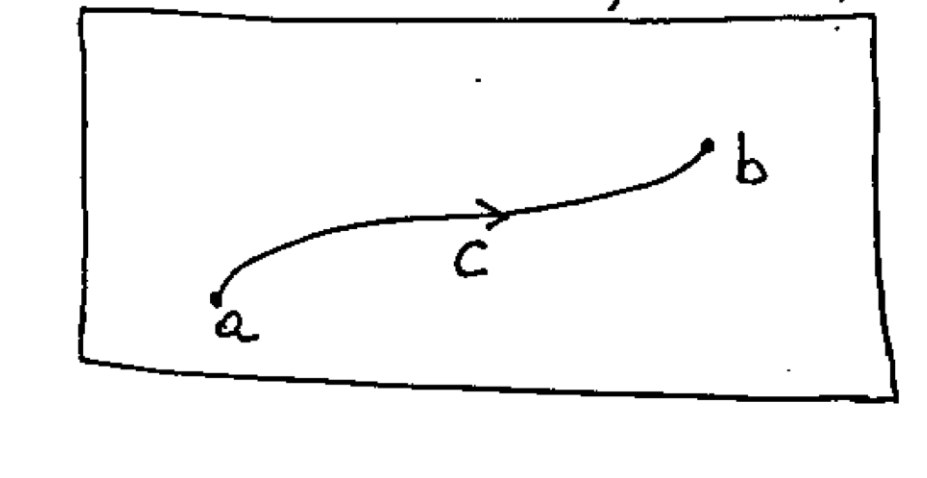
\includegraphics[width=0.4\textwidth]{images/p4821.png}
\end{center}

% --- pagina 483 ---

Si supponga inoltre che esista una funzione analitica polidroma avente punti di
diramazione in $a$ e $b$ e tale che (per una sua determinazione alla quale si
riferiscono le considerazioni seguenti; o equivalentemente, su un certo foglio
della sua superficie di Riemann, foglio sul quale supporremo nel seguito di
mantenerci), tirando il taglio da $a$ a $b$ lungo la curva $C$, si abbia
\[
    \mathrm{dis}_C\left[W(z)\right] = \nu(z),
\]
dove con la notazione $\mathrm{dis}_C\left[W(z)\right]$ si è indicata la
discontinuità della funzione $w(z)$ attraverso il taglio $C$, cioè
\[
    \mathrm{dis}_C\left[W(z)\right] = W(z_+) - W(z_-),
\]
dove $z_+$ e $z_-$ indicano due punti l'uno dirimpetto all'altro sui due bordi
del taglio $C$:

\begin{center}
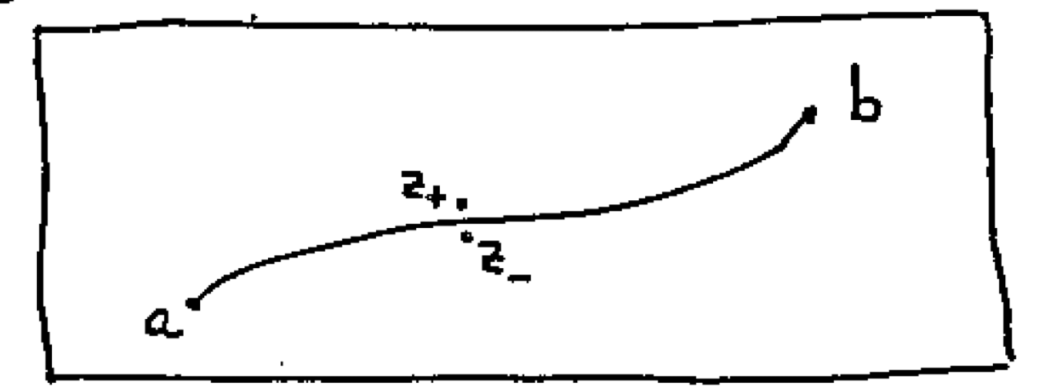
\includegraphics[width=0.4\textwidth]{images/p4831.png}
\end{center}

È allora chiaro che si può scrivere
\[
    I = \int_{C'} dz\;W(z)
\]
essendo la curva chiusa $C'$ quella indicata in figura

\begin{center}
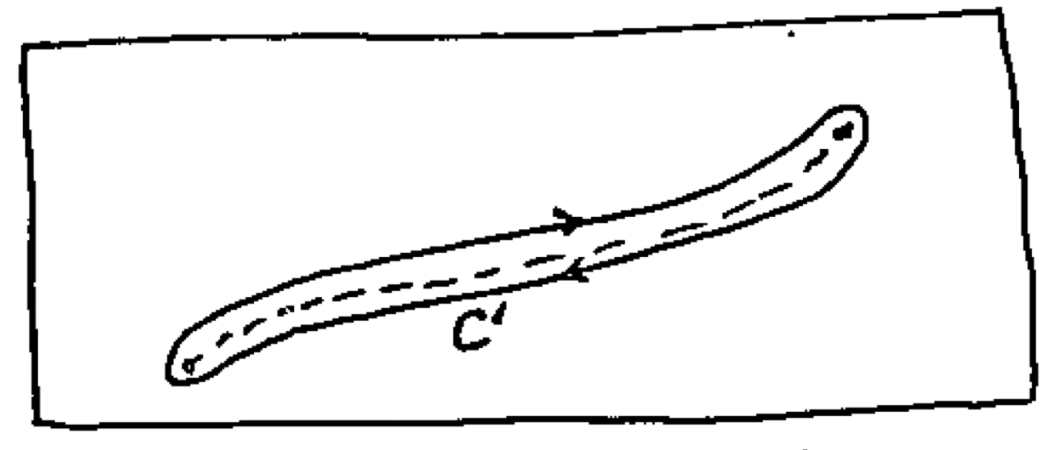
\includegraphics[width=0.4\textwidth]{images/p4832.png}
\end{center}

Naturalmente tale curva $C'$ dovrebbe a rigore essere ``infinitamente vicina''
alla curva $C$ --- indicata nella figura a tratto interrotto --- ma sappiamo che
in realtà può anche allontanarsene a piacere --- essere cioè sostituita da
un'altra curva chiusa $C''$

\begin{center}
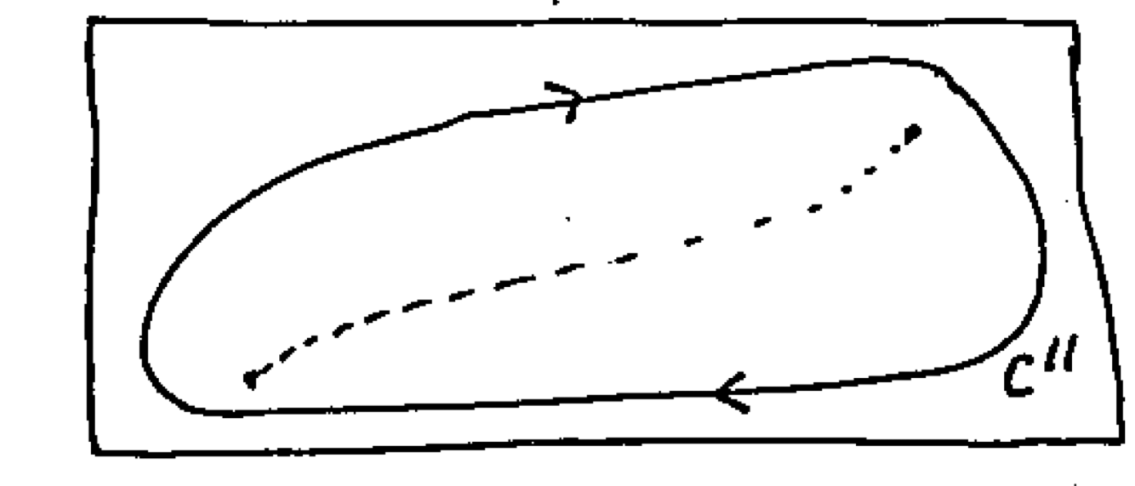
\includegraphics[width=0.4\textwidth]{images/p4833.png}
\end{center}

a condizione che nella zona racchiusa da tale curva non cadano altre singolarità
di $w(z)$ (oltre ai due punti di diramazione in $a$ e $b$).

Inoltre a rigore la curva $C'$ contiene due pezzetti ``in più'', cioè
i due semicerchi intorno agli estremi che servono a chiudere il contorno;

% --- pagina 484 ---

ma data la lunghezza infinitesima di tali cerchietti (infinitesima in quanto
supponiamo che $C'$ sia infinitamente vicina a $C$), i loro contributi al valore
complessivo dell'integrale saranno generalmente trascurabili; questo è però un
punto da controllare caso per caso (si ricordi peraltro che il comportamento
dell'integrando nei dintorni di $a$ e $b$ non può essere del tutto arbitrario,
se si vuole che l'integrale di partenza sia convergente).

È molto importante osservare che non si è richiesto alla $\nu(z)$ di
essere analitica; basta che lo sia la $w(z)$.

Naturalmente il discorso testé svolto risulterà, dal punto di vista
applicativo, particolarmente interessante, se la curva $C$ di partenza giace
sull'asse reale, di modo che l'integrale di partenza è un integrale di variabili
reale.

Sarà inoltre particolarmente interessante il caso in cui la curva $C$
--- anziché essere di lunghezza limitata, come indicato nelle figure --- si
estenda all'infinito (da una, o da ambedue le parti). Considerazioni del tutto
analoghe a quelle fin qui svolte si possono estendere a tale caso, salvo
naturalmente assicurarsi la convergenza degli integrali in questione; con in più
la possibilità, sotto opportune condizioni, di richiudere i contorni di
integrazione con degli archi di cerchio ``di raggio infinito'', che forniscono
contributi nulli se, nei settori del piano complesso rilevanti in ciascun caso,
l'integrando $w(z)$ si annulla per $z \to \infty$ (in modo sufficientemente
rapido, cioè più rapidamente di $|z|^{-1}$).

\medskip
Dopo questa discussione che ha illustrato in termini generali l'idea-base
di queste tecniche di calcolo, passiamo senz'altro all'analisi di qualche classe
di integrali effettuabili mediante tecniche di questo tipo, non senza sottolineare
che la tecnica è ovviamente assai generale e può essere utilmente impiegata anche
in molti altri casi, diversi da quelli che verranno esplicitamente illustrati qui.

L'esempio principale che vogliamo considerare è quello dell'integrale
\begin{equation}
    I = \int_0^\infty dx\; x^c\, R(x), \tag{1}
\end{equation}
con $c$ costante complessa e $R(x)$ funzione \underline{razionale}. La razionalità
di $R(x)$ implica che, per $x \to 0$,
\begin{equation}
    R(x) = c'\, x^p \left[1 + O(x)\right], \tag{2}
\end{equation}
e per $x \to \infty$
\begin{equation}
    R(x) = c''\, x^q \left[1 + O(x)\right], \tag{3}
\end{equation}
con $p$ e $q$ interi e $c'$ e $c''$ costanti non nulle (in generale, complesse).
Affinché l'integrale $I$ esista (converga), dovranno inoltre valere le disuguaglianze

% --- pagina 485 ---

\begin{equation}
    -1-p < \mathrm{Re}(c) < -1-q \tag{4}
\end{equation}
che supporremo dunque soddisfatte.

Assumiamo inoltre che i poli di $R(z)$ non cadano sull'asse reale positivo
(salvo eventualmente in $z=0$; il comportamento consentito di $R(x)$ per
$x \to 0$ è stato già discusso, risultando poli in $z=0$ ammessi o esclusi a
seconda che $\mathrm{Re}(c) > 0$ o $\mathrm{Re}(c) < 0$).

Questa condizione è ovviamente anche richiesta affinché l'integrale $I$,
eq.~(1), risulti convergente.

Sotto queste ipotesi, risulta allora assai facile dimostrare che la
valutazione dell'integrale $I$ di eq.~(1) si riduce ad una somma su un numero
finito di residui, e precisamente
\begin{equation}
    \int_0^\infty dx\; x^c\, R(x) = -\left[\pi e^{-i\pi c}/\sin(\pi c)\right]
    \sum_k \mathrm{Res}_k\!\left[z^c R(z)\right], \tag{5}
\end{equation}
essendo la somma estesa, come suggerito dalla notazione usata, ai residui di
tutti i poli della funzione
\begin{equation}
    W(z) = z^c\, R(z). \tag{6}
\end{equation}

Come è ovvio, questa funzione è, a parte i due punti di diramazione in
$z=0$ e $z=\infty$, una funzione analitica di $z$, avente un numero finito di
poli la cui posizione coincide con la posizione dei poli di $R(z)$ (ovverosia
con quella degli zeri del polinomio a denominatore di $R(z)$), ed i cui residui
coincidono (nel caso di poli semplici) con i residui di $R(z)$ moltiplicati per
$(z_k)^c$, ove $z_k$ è la posizione di ciascun polo e la determinazione di
$(z_k)^c$ che deve essere scelta è
\begin{equation}
    (z_k)^c = (\rho_k)^c\, e^{i\theta_k c} \tag{7}
\end{equation}
ove $\rho_k$ e $\Theta_k$ sono rispettivamente modulo e fase di $z_k$,
\begin{equation}
    z_k = \rho_k\, e^{i\Theta_k}, \tag{8}
\end{equation}

% --- pagina 486 ---

con la convenzione
\begin{equation}
    0 < \Theta_k < 2\pi \tag{9}
\end{equation}
(non vi sono segni di uguaglianza in quanto sappiamo per ipotesi che i poli
di $R(z)$ non possono cadere sull'asse reale).

\medskip
\noindent\underline{esercizio}\quad Indichiamo brevemente come si dimostra la (5),
lasciando come per il lettore una più rigorosa giustificazione dei vari passaggi.
Consideriamo anzitutto l'integrale
\[
    J = \int_C dz\; z^c\, R(z)
\]
esteso alla curva chiusa $C$ schematicamente indicata nella figura, supponendo
inoltre che il raggio $R$ del semicerchio sia stato scelto sufficientemente grande
da assicurare che entro $C$ cadano tutti i poli dell'integrando

\begin{center}
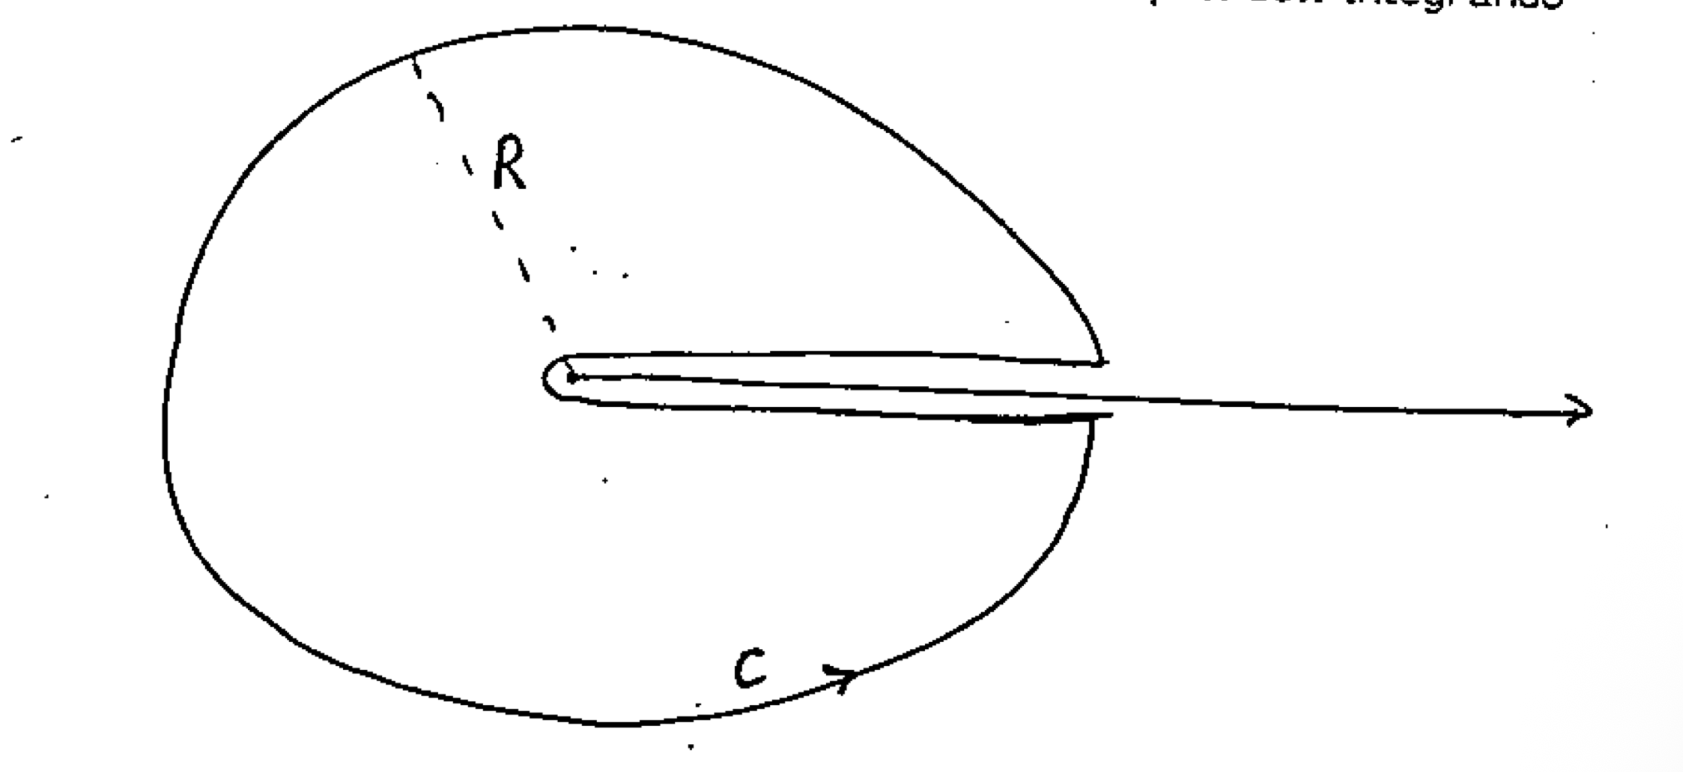
\includegraphics[width=0.45\textwidth]{images/p4861.png}
\end{center}

Si intende che i due rami della curva $C$ che corrono lungo l'asse reale siano
``infinitamente vicini''.

È allora chiaro, per il teorema dei residui, che
\[
    J = 2\pi i \sum_k \mathrm{Res}_k\!\left[z^c R(z)\right].
\]
Perché supponiamo --- vedi sotto --- di considerare la funzione $z^c$ nel piano
complesso tagliato lungo il semiasse reale positivo, da $z=0$ a $z=\infty$, e
di considerarne dunque quella determinazione per cui
\[
    z^c = \rho^c\, e^{i\theta c}
\]
essendo
\[
    z = \rho\, e^{i\theta}
\]
con
\[
    0 \leq \theta \leq 2\pi,
\]

% --- pagina 487 ---

i residui andranno calcolati secondo le prescrizioni indicate più sopra
(vedi in particolare le eq.~(7), (8) e (9)).

Si osservi che questa determinazione della funzione $z^c$ non è la più
usuale, che richiederebbe invece di tagliare il piano complesso lungo il
semiasse reale negativo. La scelta adottata qui è peraltro altrettanto lecita
quanto qualunque altra, purché la stessa convenzione venga adottata con
coerenza anche nei passaggi successivi.

Il cammino $C$ può d'altronde essere spezzato in 4 parti: un semicerchio
di raggio infinitesimo intorno a $z=0$, che dà chiaramente un contributo
trascurabile (per la disuguaglianza di sinistra delle (4)) e può pertanto essere
ignorato; un cerchio di raggio $R$, che dà un contributo trascurabile nel limite
in cui tale raggio $R$ diverge, a causa dell'annullarsi, più rapidamente di
$R^{-1}$, dell'integrando (per la disuguaglianza di sinistra delle (4)); un
integrale esteso al bordo superiore del taglio, che nel limite $R \to \infty$
coincide proprio con l'integrale $I$ di eq.~(1), poiché nel bordo superiore del
taglio, per la determinazione di $z^c$ che si è convenuto di scegliere,
$z^c = [\rho \, e^{i\theta}]^c = \rho^c = x^c$; un integrale esteso al bordo
inferiore del taglio, che nel limite $R \to \infty$ varrà $-e^{2\pi i c}\, I$,
poiché per la determinazione di $z^c$ che si è scelta, nel bordo inferiore del
taglio $z^c = [\rho\, e^{2\pi i}]^c = x^c e^{2\pi i c}$ (il segno meno origina
dal fatto che, lungo il bordo negativo, il verso di percorrenza dell'integrale è
--- vedi figura --- opposto a quello che si ha nella definizione (1) di $I$, in
cui si integra da $0$ a $\infty$).

Sicché in conclusione si ottiene
\[
    J = \left[1 - e^{2\pi i c}\right] I = -2i\, e^{\pi i c}\sin(\pi c)\, I \,.
\]
Questa equazione, confrontata con la precedente espressione di $J$, fornisce
per l'appunto la formula (5) che si voleva dimostrare.

\medskip
La formula (5) può anche scriversi, con ovvia notazione, nella forma
\begin{align}
    \int_0^\infty dx\; e^{c \ln x}\, R(x) &= -\pi\left[\sin(\pi c)\right]^{-1} \notag\\
    &\quad \cdot \sum_k \mathrm{Res}_k\!\left\{e^{c(-i\pi + \log z)}\, R(z)\right\}, \tag{10}
\end{align}
indicando $\log z$ la determinazione principale del logaritmo (vedi la sezione
precedente); la somma va estesa su tutti i poli di $R(z)$.

Sviluppando in serie di potenze di $c$ ambo i membri di questa equazione
ed uguagliando i termini che corrispondono alla stessa potenza, si ottengono
le relazioni
\begin{equation}
    0 = \sum_k \mathrm{Res}_k\!\left[R(z)\right], \tag{11}
\end{equation}
\begin{equation}
    \int_0^\infty dx\; R(x) = -\sum_k \mathrm{Res}_k\!\left[\log z\, R(z)\right], \tag{12}
\end{equation}

% --- pagina 488 ---

\begin{equation}
    \int_0^\infty dx\; \log x\; R(x) = -\tfrac{1}{2}\sum_k \mathrm{Res}_k\!\left\{
    \left[-i\pi + \log z\right] R(z)\right\}, \tag{13}
\end{equation}
\begin{align}
    \int_0^\infty dx\;(\log x)^2\, R(x) &= -\tfrac{1}{3}\sum_k \mathrm{Res}_k\!\Bigl\{
    \bigl[\pi^2 \log z \notag\\
    &\quad + (-i\pi + \log z)^3\bigr]\, R(z)\Bigr\}, \tag{14}
\end{align}
e così via.

Infatti se si pone
\[
    t/\sin t = \sum_{n=0}^\infty a_n\, t^n, \quad |t| < \pi,
\]
si ha ovviamente
\begin{align}
    \pi\left[\sin(\pi c)\right]^{-1} e^{\alpha c}
    &= \sum_{\ell=-1}^\infty a_{\ell+1}\, \pi^{\ell+1} c^\ell
       \Biggl(\sum_{m=0}^\infty \alpha^m c^m / m!\Biggr) \notag\\
    &= \sum_{n=-1}^\infty c^n \sum_{m=0}^{n+1} a_{n-m+1}\, \pi^{n-m+1}\, \alpha^m / m!
\end{align}
(il secondo passaggio è ottenuto ponendo $\ell + m = n$). Pertanto la formula
generale sarà
\begin{align}
    \int_0^\infty dx\; (\log x)^n\, R(x) &= -n!\sum_k \mathrm{Res}_k\Biggl\{R(z)\cdot \notag\\
    &\quad \cdot \sum_{m=0}^{n+1} a_{n-m+1}\,\pi^{n-m+1}(-i\pi+\log z)^m / m!\Biggr\}
\end{align}
per $n = 0, 1, 2, 3, \ldots$\;. La (11) corrisponde ad $n = -1$, ed esprime una
proprietà dei residui di una funzione razionale (più in generale, monodroma)
tale da annullarsi più rapidamente di $|z|^{-1}$ per $z \to \infty$ in ogni
direzione nel piano complesso, proprietà che discende ovviamente --- come si
era del resto già visto (\underline{esercizio 6-7}) --- dal teorema dei residui.

I coefficienti $a_n$ sono ovviamente nulli se $n$ è dispari; per $n$ pari
i primi 5 di questi coefficienti sono dati qui di seguito:
\[
    a_0 = 1,\quad a_2 = 1/6,\quad a_4 = 7/360,\quad a_6 = 31/15120,\quad
    a_8 = 127/604800\,.
\]
Si verifichino \underline{per esercizio}, usando questi coefficienti, le equazioni
(12) (13) e (14) (si noti che entrano solo $a_0$ ed $a_2$).

\medskip
Le equazioni (12), (13), (14) etc.\ potrebbero essere ricavate, anziché
mediante lo sviluppo in serie della (10), direttamente utilizzando una tecnica
di calcolo analoga a quella impiegata più sopra, basandosi cioè sulla osservazione
che la discontinuità sul taglio --- tracciato lungo il semiasse reale positivo,
da $z=0$ a $z=\infty$ --- della funzione

% --- pagina 489 ---

\begin{equation}
    W(z) = \left(\log z\right)^n \tag{15}
\end{equation}
nel foglio corrispondente alla determinazione principale della funzione logaritmo,
è pari a
\begin{equation}
    (\log x)^n - (2\pi i + \log x)^n
    = -\sum_{m=0}^{n-1} \binom{n}{m} (2\pi i)^{n-m} (\log x)^m. \tag{16}
\end{equation}

In particolare la discontinuità di $\log z$ (come del resto già sappiamo)
è $-2\pi i$; osservazione questa che permette, in modo del tutto analogo a
quello usato precedentemente, di effettuare l'integrale
\begin{equation}
    I = \int_0^\infty dx\; (-2\pi i)\, R(x), \tag{17}
\end{equation}
ottenendo così la (12). Inoltre la discontinuità di $\log^2 z$ è
$4\pi^2 - 4\pi i \log x$; osservazione questa che permette di effettuare,
sempre con la stessa tecnica, l'integrale
\begin{equation}
    I = \int_0^\infty dx\; (4\pi^2 - 4\pi i \log x)\, R(x), \tag{18}
\end{equation}
ottenendone, anche con l'ausilio della (12), la (13). E così via di seguito.

\medskip
Si riottengano \underline{per esercizio} le formule (12), (13) e (14) usando la
procedura testé descritta; e si ricavi per questa via la formula generale che
fornisce il valore dell'integrale
\[
    \int_0^\infty dx\; (\log x)^n\, R(x)
\]
per $n$ intero positivo, confrontando il risultato ottenuto con quello fornito
più sopra.

\medskip
Un'altra classe di integrali il cui calcolo è riconducibile a quello
dell'integrale $I$ di eq.~(1) è
\begin{equation}
    J = \int_a^b dx\; \left[(x-a)/(b-x)\right]^c R(x), \quad b > a. \tag{19}
\end{equation}
In effetti, integrali di questo tipo prendono la forma di eq.~(1) se si effettua
il cambiamento di variabile

% --- pagina 490 ---

\begin{align}
    t &= (x-a)/(b-x), \tag{20a}\\
    x &= (a+bt)/(1+t), \tag{20b}
\end{align}
che fornisce
\begin{equation}
    J = (b-a)\int_0^\infty dt\; t^c\, Q(t) \tag{21}
\end{equation}
con
\begin{equation}
    Q(t) = (1+t)^{-2}\, R\!\left[(a+bt)/(1+t)\right]. \tag{22}
\end{equation}
Si noti che, se $R(x)$ è razionale, lo sarà anche $Q(t)$.

In modo analogo lo stesso cambiamento di variabile permette di ricondurre
ai casi trattati precedentemente integrali del tipo
\[
    \int_0^\infty dx\; \left\{\ln\left[(x-a)/(b-x)\right]\right\}^n R(x), \quad b > a,
\]
con $n$ intero non negativo.

\medskip
È però assai istruttivo osservare che l'integrale $J$ di eq.~(19) potrebbe
essere effettuato direttamente, secondo la tecnica illustrata in questa sezione,
a partire dalla funzione
\[
    W(z) = \left[(z-a)/(z-b)\right]^c
\]
che ha due punti di diramazione in $z=a$ e $z=b$, con discontinuità attraverso
il taglio (tracciato sull'asse reale da $a$ a $b$) nel foglio in cui $w(z)$ è
reale positivo per $z$ reale positivo e maggiore di $b$, pari a
\[
    -2i\sin(c\pi)\,\left[(x-a)/(b-x)\right]^c
\]
(vedi l'esercizio 9-5).

\medskip
Nella discussione fin qui svolta si è supposto che la funzione $R(x)$
fosse razionale. È peraltro ovvio che i risultati si estendono immediatamente
ad ogni funzione $f(x)$ che sia continuabile analiticamente, la cui continuazione
analitica $f(z)$ sia monodroma in tutto il piano complesso, priva di punti
singolari non isolati, e il cui comportamento asintotico per $z \to \infty$ in
ogni direzione nel piano complesso sia tale da permettere di trascurare il
contributo degli integrali estesi ad archi di cerchio di raggio divergente;
per esempio, nel caso dell'integrale $I$ della eq.~(1), rimpiazzando

% --- pagina 491 ---

$R(x)$ con $f(x)$ si avrebbe la condizione
\begin{equation}
    \lim_{z \to \infty} \left[z^{-1+\varepsilon+\mathrm{Re}\, c}\, f(z)\right] = 0 \tag{23}
\end{equation}
che deve valere per qualche $\varepsilon$ positivo, ancorché piccolo, e per
$z \to \infty$ lungo qualunque direzione nel piano complesso.

\begin{esercizi}
\item Si dia la generalizzazione della formula (5) nella ipotesi che uno (o più)
    poli della funzione $R(x)$ cadano entro l'asse reale positivo, e che la
    definizione (1) dell'integrale $I$ sia rimpiazzata da
    \[
        I = \mathrm{P}\int_0^\infty dx\; x^c\, R(x)
    \]
    riferendosi ovviamente la prescrizione di valor principale a tutti i poli
    che cadono sull'asse reale.

\item Si dimostri la formula
    \[
        \int_0^\infty dx\; x^{c-1}/(1+x) = \pi/\sin(\pi c),
    \]
    valida per $0 < \mathrm{Re}\, c < 1$.

\item Si consideri la funzione
    \[
        W(z) = \int_0^\infty dt\; e^{z \log t} / \left[t(1+t)\right],
    \]
    che è chiaramente analitica nella striscia del piano complesso $z$ caratterizzata
    dalla limitazione $0 < \mathrm{Re}\, z < 1$. Si dimostri che tale funzione
    analitica $W(z)$ è analiticamente continuabile al di fuori di tale striscia, e
    si calcoli il valore di tale continuazione analitica nel punto $z = 3/2$. Si
    dimostri inoltre che tale continuazione è monodroma in tutto il piano complesso
    e se ne discutano le singolarità.

\item Si dimostri la formula (valida per $0 < \mathrm{Re}\, c < 1$)
    \[
        \int_0^1 dt\; t^{c-1}(1-t)^{-c} = \pi/\sin(\pi c).
    \]

\item Si valutino i seguenti integrali:
    \begin{enumerate}
        \item[(i)] $I = \displaystyle\int_0^\infty dx\; (1+x^2)^{-2} \log x$;
        \item[(ii)] $I = \displaystyle\int_0^\infty dx\; x^c/(1+x^2)$;
        \item[(iii)] $I = \displaystyle\int_0^\infty dx\; x^c/(1+x^2)^2$;
        \item[(iv)] $I = \displaystyle\int_0^\infty dx\; x^c/(1+2x\cos\lambda+x^2)$, $-\pi < \lambda < \pi$;
        \item[(v)] $I = \displaystyle\int_0^1 dx\; x^{1-c}(1-x)^c/(1+x^3)$;
        \item[(vi)] $I = \displaystyle\int_0^1 dx\; x^{1-c}(1-x)^c/(1+x^2)$;
        \item[(vii)] $I = \displaystyle\int_0^1 dx\; x^{1-c}(1-x)^c/(1+x)^2$;
        \item[(viii)] $I = \displaystyle\int_{-1}^1 dx\; (1+x)^{1-c}(1-x)^c/(1+x^2)$.
    \end{enumerate}
    In queste formule $c$ indica una costante complessa. Si indichi in ciascun
    caso a quali limitazioni deve soddisfare $c$ affinché gli integrali risultino
    convergenti.

\item Si valuti l'integrale
    \[
        I(c) = \mathrm{P}\int_{-1}^1 dx\; (x-c)^{-1}(1-x^2)^{-1/2}
    \]
    dove $c$ è una costante complessa, arbitraria salvo per la limitazione
    $c \neq \pm 1$, e la prescrizione di valor principale si riferisce al caso
    in cui $c$ sia reale e $-1 < c < +1$. In particolare si valuti la funzione
    $I(c)$ nei punti $c = e^{\pm i\theta}$ con $0 \leq \theta < \pi$, nei punti
    $c = ia$ con $a$ reale, e per $c$ reale e compreso fra $-1$ ed $1$ (nel quale
    ultimo caso vale la prescrizione di valor principale).

\item Si valutino i seguenti integrali (essendo $a$ una costante reale non nulla):
    \begin{enumerate}
        \item[(i)] $I = \displaystyle\int_0^\infty dx\; (\log x)/(x^2+a^2)$;
        \item[(ii)] $I = \displaystyle\int_0^\infty dx\; (\log x)^2/(x^2+a^2)$.
    \end{enumerate}
\end{esercizi}

\section{Causalità ed analiticità}

Già nella sezione 8 si era vista --- o almeno intravista --- una relazione fra
proprietà di analiticità e causalità (in connessione con lo studio delle funzioni
di Green). In questa sezione vogliamo riprendere l'argomento, senza alcuna pretesa
di approfondimento, ma con l'intento almeno di introdurre l'idea-base, i cui
sviluppi giuocano un ruolo di fondamentale importanza in molti campi della fisica
--- dalle telecomunicazioni alla teoria delle (cosiddette) particelle elementari.

Si consideri un fenomeno fisico --- relazione di causa ed effetto ---
descrivibile mediante la seguente equazione
\begin{equation}
    g(t) = \int_{-\infty}^t dt'\; S(t,t')\, f(t'). \tag{1}
\end{equation}
In questa equazione le variabili $t$, $t'$ indicano dei tempi; $f(t)$ è la
funzione del tempo che descrive la causa, $g(t)$ la funzione del tempo che
descrive l'effetto, $S(t,t')$ è la funzione che descrive il sistema fisico
caratterizzante la relazione di causa ed effetto.

% --- pagina 493 ---

Per esempio $f(t)$ potrebbe descrivere la tensione di entrata in un
apparato elettronico, $g(t)$ quella di uscita:

\begin{center}
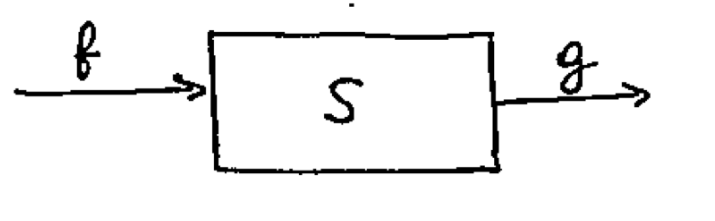
\includegraphics[width=0.35\textwidth]{images/p4931.png}
\end{center}

Il fenomeno fisico descritto dalla (1) è lineare (cioè, se $f_1$ produce
$g_1$ ed $f_2$ produce $g_2$, allora $f_1 + f_2$ produce $g_1 + g_2$ --- poiché,
nella (1), $S$ non dipende da $f$); questa formidabile semplificazione non è del
tutto essenziale per quel che segue, ma verrà nondimeno mantenuta.

Il fenomeno fisico descritto dalla (1) è inoltre \underline{causale}; la struttura
della (1) implica infatti che il valore $g(t)$ di $g$ al tempo $t$ può dipendere
solo dai valori assunti da $f(t')$ per $t' \leq t$, ma non dai valori di
$f(t')$ per $t' > t$.

Questa proprietà può essere, in modo del tutto equivalente, evidenziata
scrivendo, in luogo della (1),
\begin{equation}
    g(t) = \int_{-\infty}^{+\infty} dt'\; S(t,t')\, f(t'), \tag{2}
\end{equation}
ma richiedendo alla funzione $S(t,t')$ di soddisfare alla \underline{condizione di causalità}
\begin{equation}
    S(t,t') = 0 \quad \text{per} \quad t' > t. \tag{3}
\end{equation}

Questa seconda formulazione, pur essendo ovviamente del tutto equivalente
alla (1), ha il pregio di attribuire formalmente la proprietà di causalità alla
funzione $S(t,t')$ che è per l'appunto quella che descrive il sistema fisico che
realizza la connessione fra ``causa'' $f(t)$ ed ``effetto'' $g(t)$.

Scopo di questa sezione è mostrare come a questa fondamentale proprietà
corrisponda una semplice proprietà di analiticità della trasformata di Fourier
della funzione $S(t,t')$.

Le proprietà della trasformata di Fourier di $S(t,t')$ ci interessano,
in quanto il passaggio allo spazio di Fourier è spesso il modo più conveniente
per studiare (``risolvere'') la (1). Infatti ponendo

% --- pagina 494 ---

\begin{align}
    f(t) &= \int_{-\infty}^{+\infty} \frac{dk}{2\pi}\; e^{ikt}\, \hat{f}(k), \tag{4}\\
    g(t) &= \int_{-\infty}^{+\infty} \frac{dk}{2\pi}\; e^{ikt}\, \hat{g}(k), \tag{5}
\end{align}
e
\begin{equation}
    S(t,t') = \int_{-\infty}^{+\infty}\int_{-\infty}^{+\infty}
    \frac{dk}{2\pi}\,\frac{dp}{2\pi}\; e^{ikt - ipt'}\, \hat{S}(k,p) \tag{6}
\end{equation}
(il segno $-$ nel secondo esponente è convenzionale) si ottiene
\begin{equation}
    \hat{g}(k) = \int_{-\infty}^{+\infty} \frac{dp}{2\pi}\; \hat{S}(k,p)\,\hat{f}(p). \tag{7}
\end{equation}

\medskip
\noindent\textit{Derivazione dalla (7):}
\begin{align*}
\hat{g}(k) &= \int_{-\infty}^{+\infty} dt\; e^{-ikt}\, g(t) \quad \text{(per la (5,6--5))}\\
&= \int_{-\infty}^{+\infty} dt\; e^{-ikt} \int_{-\infty}^{+\infty} dt'\; S(t,t')\, f(t') \quad \text{(per la (2))}\\
&= \int_{-\infty}^{+\infty} dt\; e^{-ikt} \int_{-\infty}^{+\infty} dt' \int_{-\infty}^{+\infty}\frac{dk'}{2\pi}
   \int_{-\infty}^{+\infty}\frac{dp}{2\pi}\; e^{ik't - ipt'} \\
&\quad \cdot \hat{S}(k',p) \int_{-\infty}^{+\infty}\frac{dk''}{2\pi}\; e^{ik''t'}\hat{f}(k'') \quad \text{(per le (6) e (4))}\\
&= \int_{-\infty}^{+\infty}\frac{dk'}{2\pi}\int_{-\infty}^{+\infty}\frac{dp}{2\pi}
   \int_{-\infty}^{+\infty}\frac{dk''}{2\pi}\; 2\pi\delta(k-k')\cdot 2\pi\delta(p-k'')\\
&\quad \cdot \hat{S}(k',p)\,\hat{f}(k'') \quad \text{(per la (6.1--25a))}\\
&= \int_{-\infty}^{+\infty}\frac{dp}{2\pi}\;\hat{S}(k,p)\,\hat{f}(p) \quad \text{(per la (6.1--1)).}
\end{align*}

\medskip
L'equazione (7) è analoga alla (2); diventa però molto più semplice se
la funzione $S(t,t')$ che compare nella (2) dipende solo dalla differenza $t-t'$
(e non separatamente da $t$ e $t'$), come certo avviene se il sistema preso in
considerazione ha la proprietà di non cambiare col passare del tempo (e cioè
``invariante per traslazione temporale'').

\medskip
Infatti se $S(t,t') = S(t-t')$

% --- pagina 495 ---

dalla (2) segue
\[
    g(t) = \int_{-\infty}^{+\infty} dt'\; S(t-t')\, f(t'),
\]
e questa implica che, se $f(t')$ è rimpiazzato da $f(t'+a)$, $g(t)$ risulta
rimpiazzato da $g(t+a)$, poiché
\[
    \int_{-\infty}^{+\infty} dt'\; S(t-t')\, f(t'+a) = \int_{-\infty}^{+\infty} dt''\; S(t+a-t'')\, f(t'').
\]
Ma la proprietà testé descritta, e sintetizzata dalla formula
\[
    g(t+a) = \int_{-\infty}^{+\infty} dt'\; S(t,t')\, f(t'+a)
\]
è per l'appunto quel che si intende quando si afferma che il sistema che
trasforma la ``causa'' in ``effetto'' non dipende dal tempo: uguali cause, di
cui una ritardata rispetto all'altra di un intervallo di tempo $a$, producono
``effetti'' uguali salvo per un analogo ritardo di un intervallo di tempo $a$.

\medskip
La proprietà di $S(t,t')$ di dipendere solo dalla differenza $t-t'$ implica
in effetti, per la trasformata di Fourier $\hat{S}(k,p)$, la proprietà
\begin{equation}
    \hat{S}(k,p) = \hat{S}(k)\; 2\pi\,\delta(k-p) \tag{8}
\end{equation}
(il fattore $2\pi$ è ovviamente convenzionale).

Infatti la (8), inserita nella (6), fornisce
\[
    S(t,t') = \int_{-\infty}^{+\infty}\frac{dk}{2\pi}\; e^{ik(t-t')}\,\hat{S}(k)
\]
implica cioè che $S(t,t')$ dipende solo dalla differenza $t-t'$.

Inserendo la (8) nella (7), si ottiene
\begin{equation}
    \hat{g}(k) = \hat{S}(k)\,\hat{f}(k), \tag{9}
\end{equation}
che mostra appunto come, nel caso in cui il sistema sia lineare e indipendente
dal tempo, la trasformata di Fourier $\hat{g}(k)$ dell'``effetto'' $g(t)$ si
ottenga dalla trasformata di Fourier $\hat{f}(k)$ della ``causa'' $f(t)$ tramite
una semplice moltiplicazione per la funzione $\hat{S}(k)$ caratterizzante la
(trasformata di Fourier del) sistema.

Il risultato (9) è ben noto; mostra come --- sotto le ipotesi fatte sinora,
e cioè linearità e invarianza temporale --- tutta l'informazione fi-

% --- pagina 496 ---

sica sul sistema risulti nel modo più semplice e conveniente sintetizzata nella
funzione $\hat{S}(k)$.

Il problema ancora aperto, e la cui analisi è in effetti il nostro
obbiettivo principale, è quello di chiarire quale restrizione sulla funzione
$\hat{S}(k)$ risulti dalla proprietà di causalità (3). Osserviamo anzitutto che
se vale come ora supponiamo l'ipotesi di invarianza temporale, la funzione $S$
dipende in realtà da una sola variabile, (per esempio) che possiamo indicare
con la lettera $\tau$, ed è legata alla $\hat{S}(k)$ dalla relazione
\begin{equation}
    S(\tau) = \int_{-\infty}^{+\infty} \frac{dk}{2\pi}\; e^{ik\tau}\,\hat{S}(k). \tag{10}
\end{equation}
Quanto alla proprietà di causalità (3), essa si scriverà ora nella forma
\begin{equation}
    S(\tau) = 0 \quad \text{per} \quad \tau < 0. \tag{11}
\end{equation}

Ebbene è assai facile mostrare che, sotto ipotesi abbastanza generali
(concernenti il comportamento asintotico della $\hat{S}(k)$ per $k$ complesso;
vedi sotto), la proprietà di causalità (11) per la $S(\tau)$ risulta assicurata
se \underline{la funzione $\hat{S}(k)$}, originariamente definita per $k$ reale, è
\uline{analiticamente continuabile ed è analitica} (cioè priva di singolarità)
\uline{in tutto il semipiano inferiore del piano complesso $k$} (nel semipiano
caratterizzato cioè dalla relazione $\mathrm{Im}\, k \leq 0$).

\medskip
Si assuma infatti che $\hat{S}(k)$ sia continuabile analiticamente in $k$
e analitica per $\mathrm{Im}\, k \leq 0$, ed inoltre che, per qualche $\varepsilon$
positivo (magari anche molto piccolo),
\[
    \lim_{k \to \infty} \left[|k|^{1+\varepsilon}\,\hat{S}(k)\right] = 0
\]
per $k \to \infty$ in qualunque direzione nel semipiano complesso inferiore.
Allora, per $\tau < 0$, è possibile chiudere l'integrale a secondo membro della
(10) con un semicerchio, nel semipiano inferiore del piano complesso $k$, di
raggio $R$ divergente; si noti che l'esponente $ik\tau$, per $\tau$ negativo e
$\mathrm{Im}\, k < 0$, ha parte reale negativa, sicché il fattore $e^{ik\tau}$
nell'integrando non può peggiorare la convergenza a zero di tale contributo per
$R \to \infty$, anzi la renderà ancora più rapida.
Si può dunque scrivere, in luogo della (10), la formula
\[
    S(\tau) = \int_C \frac{dk}{2\pi}\; e^{ik\tau}\,\hat{S}(k)
\]
essendo $C$ il limite per $R \to \infty$ della curva chiusa indicata nella figura.

\begin{center}
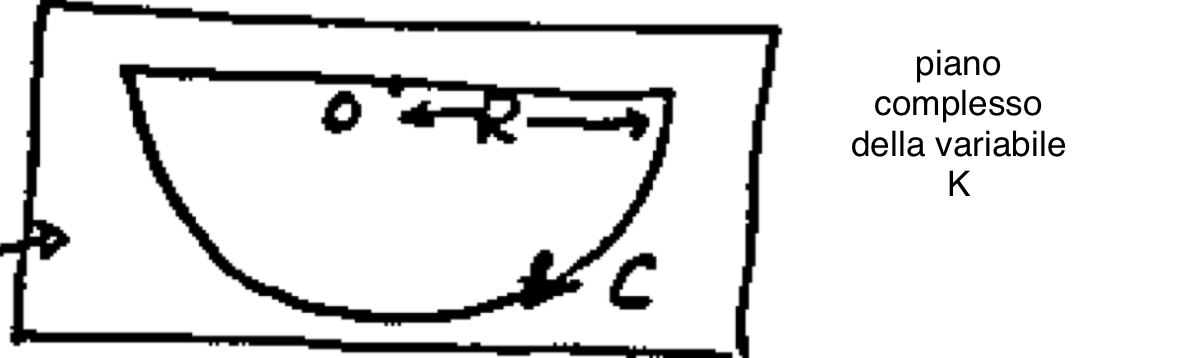
\includegraphics[width=0.35\textwidth]{images/p4961.png}
\end{center}

Ne segue allora, per il teorema di Cauchy, la conclusione \begin{center}
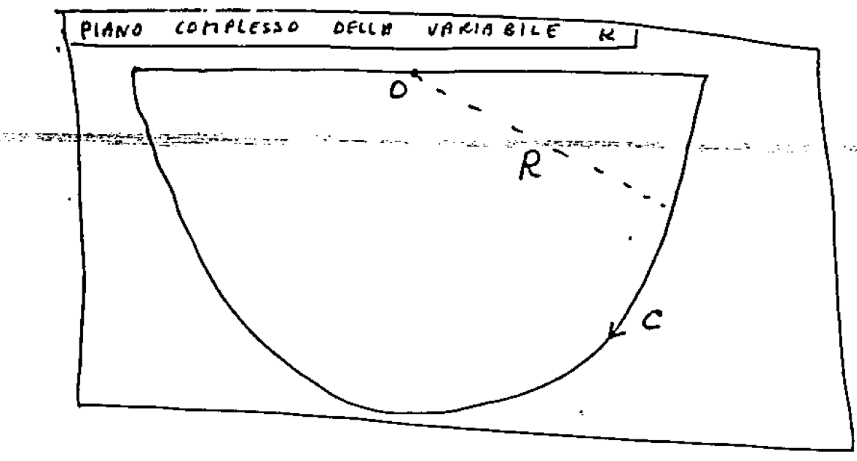
\includegraphics[width=10cm]{images/A.png}
\end{center}

$$S(\tau) = 0 \quad (\text{per } \tau \leq 0),$$

dal momento che per ipotesi nessuna singolarità dell'integrando è compresa entro il contorno di integrazione.

Si è così dimostrato che l'ipotesi sulle proprietà di analiticità della $\hat{S}(k)$ è sufficiente a garantire la validità della proprietà di causalità (11). Si noti che è anche necessaria qualche informazione sulle proprietà asintotiche della $\hat{S}(k)$, per $k$ che diverge nel semipiano inferiore del piano complesso $k$; e precisamente che sia consentito chiudere l'integrale per di sotto. In effetti si vede facilmente che la condizione data sopra è più stringente del necessario; per esempio anche se $\hat{S}(k)$ divergesse, ma solo come una potenza (con esponente finito) di $|k|$, per $\operatorname{Im} k \to -\infty$, le cose andrebbero ancora bene; purché per $\operatorname{Re} k \to \pm\infty$ (e $\operatorname{Im} k \leq 0$) $\hat{S}(k)$ si annulli più rapidamente di $|k|^{-1}$ (nel caso marginale in cui $\hat{S}(k)$ si comporta asintoticamente proprio come $|k|^{-1}$, le cose vanno generalmente ancora bene, anche se la convergenza dell'integrale a secondo membro della (10) cessa di essere assoluta).

\vspace{1em}
\hrule
\vspace{1em}

In conclusione, dopo aver reso plausibile, per il tipo di problemi fisici qui delineato, l'utilità di passare allo spazio di Fourier, abbiamo dimostrato come la proprietà di causalità --che esprime chiaramente una caratteristica assai generale e fondamentale dei sistemi fisici-- si manifesti in modo assai diretto in termini di proprietà di analiticità. L'importanza di questo risultato risiede nella sua generalità e semplicità. Una più dettagliata analisi delle specifiche applicazioni nei diversi campi della fisica -- e sono molte e varie -- esula dai confini di questo corso.

\begin{esercizi}
\item Si costruisca la funzione $S(\tau)$ caratterizzante un sistema fisico lineare, invariante per traslazioni, causale, reale (che trasformi cioè funzioni di entrata $f(t)$ reali in funzioni di uscita $g(t)$ ancora reali) e la cui trasformata di Fourier $\hat{S}(k)$ sia una funzione analitica avente la più semplice struttura compatibile con tale ipotesi.

\item Come l'esercizio precedente, ma considerando la struttura analitica più semplice dopo quella dell'esercizio precedente.

Suggerimento: la soluzione dell'esercizio precedente contiene due costanti reali arbitrarie, di cui una moltiplicativa e l'altra positiva; la soluzione di questo esercizio conterrà 3 costanti reali, di cui una moltiplicativa e le altre due positive (non 4; è dunque esclusa la semplice sovrapposizione di due soluzioni del primo esercizio).

\item Si rifletta sulla connessione fra i risultati di questa sezione e quelli delle sezioni 1.5, 1.6, 1.7, 5.9, 8.5 % [DUBBIO] riferimento poco leggibile
del capitolo 7; e in particolare si connettano le soluzioni dei due precedenti esercizi con i risultati di precedenti sezioni.
\end{esercizi}

\section*{8.S \quad Soluzioni degli esercizi del capitolo 8}

\begin{description}
\item[1-1] Le (ii), (iii), (v), (vii) non sono analitiche. Le (i) e (viii) sono analitiche per ogni valore finito di $z$; la (vi) per ogni valore di $z$ eccetto i due punti $z = \pm i$; la (iv) per ogni valore finito di $z$ eccetto $z = i(2n+1)\pi/(2y)$, $n = 0, \pm 1, \pm 2, \ldots$.

\item[2-1] Ovviamente sì.

\item[2-2] 
\begin{align*}
z^n &= (x+iy)^n \\
&= \sum_{\ell=0}^{n} \binom{n}{\ell} i^\ell y^\ell x^{n-\ell} \\
&= \sum_{j=0}^{[n/2]} \binom{n}{2j}(-1)^j y^{2j} x^{n-2j} \\
&\quad + i \sum_{j=0}^{[(n-1)/2]} \binom{n}{2j+1}(-1)^j y^{2j+1} x^{n-(2j+1)}.
\end{align*}

Il primo passaggio è stato effettuato usando la formula di Leibnitz (potenza ennesima di un binomio), il simbolo
$$\binom{n}{\ell} \equiv \frac{n!}{\ell!\,(n-\ell)!}$$
è per l'appunto il coefficiente binomiale. Il secondo passaggio è stato effettuato separando le due somme in cui l'indice $\ell$ assume valori pari o dispari; ovviamente il simbolo $[p]$ indica la parte intera del numero $p$.

I due polinomi armonici omogenei di grado $n$ nelle due variabili $x$ ed $y$ sono dunque
\begin{align*}
P_n^{(1)}(x,y) &= \sum_{j=0}^{[n/2]} (-1)^j \binom{n}{2j} y^{2j} x^{n-2j}, \\
P_n^{(2)}(x,y) &= \sum_{j=0}^{[(n-1)/2]} (-1)^j \binom{n}{2j+1} y^{2j+1} x^{n-(2j+1)}.
\end{align*}

Questi polinomi sono ovviamente indipendenti (non consideriamo il caso banale $n=0$), poiché il primo contiene solo potenze pari della $y$ (e pari o dispari della $x$, a seconda che $n$ sia pari o dispari), il secondo solo potenze dispari della $y$.

Naturalmente il diverso ruolo delle variabili $x$ ed $y$ è solo apparente; in effetti, usando la simmetria dei coefficienti binomiali secondo cui
$$\binom{n}{\ell} = \binom{n}{n-\ell}$$
è facile mostrare che, per $n$ pari
\begin{align*}
P_n^{(1)}(x,y) &\propto P_n^{(1)}(y,x), \\
P_n^{(2)}(y,x) &\propto P_n^{(2)}(x,y),
\end{align*}
e per $n$ dispari
\begin{align*}
P_n^{(1)}(y,x) &\propto P_n^{(2)}(x,y), \\
P_n^{(2)}(y,x) &\propto P_n^{(1)}(x,y).
\end{align*}

\item[2-3] Nei casi (i), (iv) e (v) le funzioni $f(x,y)$ non sono armoniche e dunque non possono fornire la parte immaginaria di una funzione analitica; nel caso (vi) la funzione $f(x,y)$ non è reale, e dunque non può certo costituire la parte immaginaria di un numero complesso (che è per definizione reale); negli altri casi le funzioni analitiche $W(z)$ aventi le $f(x,y)$ date come parti immaginarie sono:

\begin{description}
\item[(ii)] $W(z) = i z^2 + a$,
\item[(iii)] $W(z) = \dfrac{1}{2}\sin(z^2) + a$,
\item[(vii)] $W(z) = -\exp(-2iz) + a$,
\end{description}

essendo in tutte queste equazioni $a$ una arbitraria costante \underline{reale}. Indichiamo come si ottiene, per esempio, la parte reale della $W(z)$ nel caso (vii): essa risulterà data da
$$u(x,y) = u(0,0) + \int_C du$$
con
\begin{align*}
du &= u_x\, dx + u_y\, dy \\
&= f_y\, dx - f_x\, dy \\
&= 2\exp(2y)\left[\sin(2x)\, dx - \cos(2x)\, dy\right],
\end{align*}
essendo l'ultima equazione ottenuta usando la forma esplicita della funzione $f(x,y)$ ed indicando $\int_C$ l'integrale curvilineo effettuato lungo un cammino $C$ che va dal punto $(0,0)$ al punto $(x,y)$. Se la curva $C$ è formata dai due segmenti che vanno da $(0,0)$ a $(0,y)$ a $(x,y)$ otteniamo
\begin{align*}
\int_C du &= \int_0^y dy' \left\{-2\exp(2y')\cos(2x')\right\}\Big|_{x'=0} \\
&\quad + \int_0^x dx' \left\{2\exp(2y')\sin(2x')\right\}\Big|_{y'=y} \\
&= 1 - \exp(2y)\cos(2x).
\end{align*}
Pertanto
$$u(x,y) = a - \exp(2y)\cos(2x)$$
con
$$a = u(0,0) + 1$$
costante arbitraria. Si ottiene così
\begin{align*}
W(z) &= u(x,y) + i f(x,y) \\
&= a + \exp(2y)\left[-\cos(2x) + i\sin(2x)\right] \\
&= a - \exp(-2iz).
\end{align*}
Si verifica facilmente che lo stesso risultato si sarebbe ottenuto scrivendo
$$\int_C du = \int_0^x dx' \left\{-2\exp(2y')\cos(2x')\right\}\Big|_{y'=0} + \int_0^y dy' \left\{2\exp(2y')\sin(2x')\right\}\Big|_{x'=x}$$
(che equivale a scegliere come cammino $C$ i 2 segmenti da $(0,0)$ a $(x,0)$ a $(x,y)$), o anche scrivendo
$$\int_C du = 2\int_0^1 dt\, \exp(2ty)\left[x\sin(2xt) - y\cos(2xt)\right]$$
(che equivale a scegliere come cammino il segmento che va direttamente dal punto $(0,0)$ al punto $(x,y)$, segmento che è descritto, in funzione del parametro $t$ variabile nell'intervallo da 0 ad 1, dalle equazioni
$$x' = tx, \quad y' = ty,$$
che implicano ovviamente
$$dx' = x\, dt, \quad dy' = y\, dt \qquad).$$

\item[2-4] $c = \pm 2$, \quad $W(z) = +i\cos(2z) + a$, $a$ reale.

\item[2-5] $A_3(x,y) = \operatorname{Re}\left[P_3(x+iy)\right] = \dfrac{1}{2}\left[5x^3 - 15xy^2 - 3x\right]$.

\item[3-2] Il quarto integrale è una immediata conseguenza del teorema di Cauchy; da esso e dal primo seguono immediatamente il secondo e terzo (basta usare la formula $z = x + iy$). Il primo si dimostra usando il lemma di Gauss.

\item[3-3] $I_n = 0$ se $n \neq -1$, \quad $I_{-1} = 2\pi i$.

Per dimostrarlo, scegliere come particolare curva chiusa un cerchio di centro $z_0$ e raggio $\rho$, parametrizzandolo secondo la formula $z = z_0 + \rho\exp(i\theta)$, $0 \leq \theta < 2\pi$, di modo che
$$I_n = i\rho^{n+1} \int_0^{2\pi} d\theta\, \exp\left[i\theta(n+1)\right].$$

E' infatti chiaro che questo integrale è nullo per ogni valore di $n$ intero, salvo che per $n = -1$, nel qual caso ovviamente $I_{-1} = 2\pi i$. Il fatto che lo stesso risultato si otterrebbe per ogni altra curva è una conseguenza del teorema di Cauchy.

\item[3-4] $I_1 = \dfrac{2}{3}(1+i)$, \quad $I_2 = \dfrac{1}{3}(1+4i)$, \quad $I_3 = \dfrac{1}{3}(4+i)$.

\item[3-5] L'ipotesi è essenziale. Per esempio l'integrale di $W(z) = 1/z^2$ su qualunque curva chiusa (non passante per l'origine) è nullo; eppure questa funzione è singolare (cioè non analitica) in $z = 0$.

\item[4-1] $I_1 = 0$; \quad $I_2 = \dfrac{1}{2}(2\pi i)\left(\dfrac{1}{2}\right)^2 = \dfrac{1}{4}\pi i$;
$$I_3 = \frac{1}{2i}\,2\pi i\,(i/2)^3 = -\frac{1}{8}\pi i;$$
$$I_4 = 2\pi i\,(2!)^{-1}\left[\frac{d^2}{dz^2}\exp(iz)\right]_{z=0} = \frac{1}{4}\pi i;$$
$$I_5 = \frac{1}{2}\,2\pi i\,\left(-\frac{3}{2}\right)^{-2} = \frac{4}{9}\pi i;$$
$$I_6 = \frac{1}{4}\,2\pi i\,\left\{\frac{d}{dz}\left[(z-2)^{-1}\right]\right\}_{z=\frac{1}{2}} = -\frac{2}{9}\pi i.$$
Se $\rho = 3$ (anziché $\rho = 1$) $I_1$, $I_5$ e $I_6$ cambiano, gli altri restano uguali. I nuovi valori sono
$$I_1 = 8\pi i, \quad I_5 = \frac{2}{9}\pi i, \quad I_6 = 0$$
(una tecnica sistematica per il calcolo di integrali tipo $I_5$ o $I_6$ per $\rho = 3$ verrà data nella sezione 8.7).

\item[4-3] Se $a < \pi/2$, il valore massimo è $\left[(\sinh a)^2 + \sin^2 a\right]^{1/2}$; se $a \geq \pi/2$, il valore massimo è $\cosh a$. Questo risultato si ottiene cercando il massimo di $|W(z)|$ sulla frontiera del dominio dato (principio del massimo modulo di una funzione analitica); e dunque o per $z = \pm a + iy$ con $-a \leq y \leq a$, o per $z = x \pm ia$ con $-a \leq x \leq a$. Nel primo caso $|W(z)|^2 = \sinh^2 a + \sin^2 x$ assume ovviamente il suo massimo in $x = \pi/2$ (se questo valore è compreso nell'intervallo da $-a$ ad $a$), e tale massimo vale $\sinh^2 a + 1 = \cosh^2 a$; altrimenti il valore massimo viene assunto agli estremi, per $x = \pm a$, e vale $\sinh^2 a + \sin^2 a$. Nel secondo caso, $|W(z)|^2 = \sinh^2 y + \sin^2 x$ assume ovviamente il suo massimo agli estremi, per $y = \pm a$ % [DUBBIO] frase parzialmente illeggibile
e vale $\sinh^2 a + \sin^2 a$. Questo stesso risultato si poteva ottenere direttamente, osservando che per ogni $z = x + iy$, $|\sin z|^2 = \sin^2 x + \sinh^2 y$.

\item[5-1] 
\begin{description}
\item[i)] $\dfrac{\sin(cz)}{z} = \sum_{n=0}^{\infty} (-1)^n c^{2n+1} z^{2n}/(2n+1)!$, \quad $d = \infty$;
\item[ii)] $\exp(cz) = \exp(cz_0) \sum_{n=0}^{\infty} \left[c(z-z_0)\right]^n/n!$, \quad $d = \infty$;
\item[iii)] $(z+i)/(z-1) = 2 - i - \sum_{n=1}^{\infty} i^{n+1}\left[z - (i+1)\right]^n$, \quad $d = 1$; % [DUBBIO] verificare segno
\item[iv)] $z^c = \sum_{n=0}^{\infty} \binom{c}{n}(z-1)^n$, \quad $d = 1$.
\end{description}

Nella iv)
$$\binom{c}{n} = c(c-1)(c-2)\cdots\left[c-(n-1)\right]/n!$$

Se $c$ è un numero intero positivo, $c = N$, allora per $n \leq N$
$$\binom{c}{n} = \binom{N}{n} = N!/\left[n!\,(N-n)!\right],$$
e per $n > N$
$$\binom{c}{n} = 0,$$
sicché la serie di Taylor si riduce ad un polinomio di grado $N$ (e cade naturalmente la restrizione $d=1$).

Cenno a come derivare la iii) (ed ogni caso analogo); si sostituisce ovunque a $z$ l'espressione equivalente $(z - z_0) + z_0$ e poi si sviluppi in serie di potenze di $(z - z_0)$; si effettui prima lo sviluppo del denominatore, riarrangiando opportunamente ed usando la formula (serie geometrica)
$$(1+t)^{-1} = \sum_{n=0}^{\infty} (-t)^n;$$
si includano infine i termini provenienti dal numeratore, ridefinendo gli esponenti nella somma in modo opportuno.

\item[5-2] Come è facile verificare, nell'intorno di $z=0$
$$W(z) = \sum_{m=1}^{N}\left[A_m / (1 - a_m z)\right].$$

Questa formula definisce la continuazione analitica della $W(z)$ in tutto il piano complesso, ed implica che trattasi di funzione monodroma avente $M$ singolarità (per la precisione, si tratta di poli semplici) nei punti $z_m = 1/a_m$, $m = 1, 2, \ldots, M$.

\item[5-3] La rappresentazione di Borel è
$$W(z) = \frac{1}{4}\int_0^\infty dt\, \exp(-t)\left[\exp(zt) + \exp(-zt) + \exp(izt) + \exp(-izt)\right],$$
e converge entro il quadrato di vertici $(\pm 1, \pm i)$; dunque la $W(z)$ è analitica entro tale quadrato (che include il cerchio di raggio 1 centrato nell'origine, entro cui converge lo sviluppo di Taylor).

In effetti, come è ovvio,
$$W(z) = 1/(1-z^4) = \frac{1}{4}\left[(1-z)^{-1} + (1+z)^{-1} + (1-iz)^{-1} + (1+iz)^{-1}\right],$$
ed ha dunque 4 singolarità (4 poli semplici) nei 4 punti $z_1 = 1$, $z_2 = -1$, $z_3 = i$, $z_4 = -i$.

\item[5-4] Se $\varphi(z, z')$ è funzione intera di $z$ e $z'$, le uniche singolarità dell'integrando sono i punti in cui $\varphi(z, z') = 0$. Ma deformando il cammino di integrazione è possibile evitare tali singolarità (sicché $W(z)$ continua ad essere analitica), salvo nel caso delle equazioni i) o ii) (per tali valori di $z$ le singolarità dell'integrando, come funzione di $z'$, vanno negli estremi del cammino di integrazione -- e quelli il teorema di Cauchy non mi autorizza a cambiar\emph{li}\,!), o se valgono ambedue le equazioni iii) (nel qual caso si hanno due singolarità coincidenti dell'integrando; questo può verificarsi in modo tale che il cammino di integrazione da $a$ a $b$ non possa evitarle ambedue trasformandosi con continuità a partire dal segmento iniziale; in quanto viene ad essere ``pizzicato'' fra le due singolarità).

\item[6-1] Se la funzione $W(z)$ è monodroma in tutto il piano complesso, dovrà essere
$$W(z) - W(z_0) = \int_{C_1} dz'\, W'(z') = \int_{C_2} dz'\, W'(z')$$
se i cammini $C_1$ e $C_2$ partono da $z_0$ e arrivano a $z$ (evitando naturalmente le singolarità di $W(z)$). La arbitrarietà di questi cammini, e la possibilità di andare lungo l'uno e tornare lungo l'altro, implica che per ogni contorno chiuso $C$
$$\oint_C dz\, W'(z) = 0.$$

Ma poiché anche la $W'(z)$ è monodroma ed ha dunque come singolarità solo poli o singolarità essenziali, l'integrale sulla curva chiusa $C$ è proporzionale alla somma dei residui delle singolarità di $W'(z)$ che cadono entro $C$. L'annullarsi di tale integrale, e la arbitrarietà di $C$, implicano allora che tutti i residui debbono essere nulli, c.v.d.

Si noti che questo stesso risultato si ottiene anche più direttamente scrivendo lo sviluppo di Laurent della $W(z)$ intorno al generico punto $z_0$ e poi differenziando termine a termine rispetto a $z$ per ottenere lo sviluppo di Laurent di $W'(z)$ (intorno allo stesso punto $z_0$); in tale sviluppo verrà infatti a mancare il termine che dà origine al residuo.

\item[6-2]
\begin{description}
\item[i)] $[z(1-z)]^{-1} = \displaystyle\sum_{n=-1}^{\infty} z^n$, \quad $|z| < d = 1$;
\item[ii)] $[z(1-z)]^{-1} = \displaystyle\sum_{n=-1}^{\infty} (-1)^n (z-1)^n$, \quad $|z-1| < d = 1$;
\item[iii)] $[z(1-z)]^{-1} = -\displaystyle\sum_{n=2}^{\infty} z^{-n}$, \quad $1/|z| < D = 1$;
\item[iv)] $(z^2+1)^{-2} = \displaystyle\sum_{n=-2}^{\infty} i^n(n+3)\,2^{-n-4}(z-i)^n$, \quad $|z-i| < d = 2$;
\item[v)] $(z^2+1)^{-2} = \displaystyle\sum_{m=1}^{\infty} (-1)^m m\, z^{-(2m+2)}$, \quad $1/|z| < D = 1$;
\item[vi)] $z^2 \exp(c/z) = \displaystyle\sum_{n=-\infty}^{2} c^{2-n} z^n / (2-n)!$, \quad $|z| < d = \infty$;
\item[vii)] $z^2 \exp(c/z) = \displaystyle\sum_{n=-2}^{\infty} c^{2+n} z^{-n}/(2+n)!$, \quad $1/|z| < D = \infty$.
\end{description}
Si osservi che gli ultimi due sviluppi sono identici.

\item[6-3] Tutte eccetto le ultime due, che non hanno una singolarità isolata in $z=0$.

\item[6-4]
\begin{description}
\item[i)] $\operatorname{Res}(z_0 = 0) = 1$, \quad $\operatorname{Res}(z = \pm 1) = 1/2$;
\item[ii)] $\operatorname{Res}(z_0 = \pm i) = \pm 1/(4i)$;
\item[iii)] $\operatorname{Res}(z_0 = -1) = (-)^{n+1}(2n)!/\left[(n-1)!\,(n+1)!\right]$;
\item[iv)] $\operatorname{Res}(z_0 = (2k+1)\pi/2) = -1$, \quad $k = 0, \pm 1, \pm 2, \ldots$;
\item[v)] $\operatorname{Res}(z_0 = 0) = 0$ \quad per $n = \pm 1, -2, \pm 3, -4, \pm 5, -6, \ldots$
\end{description}

\item[6-6] $\operatorname{Res}(z_0 = 0) = (-)^{n/2}/(n+1)!$ \quad per $n = 0, 2, 4, 6, \ldots$.

\begin{description}
\item[i)] $I = -\pi i/\sqrt{2}$;
\item[ii)] $I = -2\pi i$;
\item[iii)] $I = -2\pi i/9$;
\item[iv)] $I = 2\pi i$; % [DUBBIO] valore molto poco leggibile
\item[v)] $I = 0$;
\item[vi)] $I = 0$;
\item[vii)] $I = 32\pi i$;
\item[viii)] $I = 2^{n+2}\pi i/(n+1)!$ \quad per $n = -1, 0, 1, 2, 3, \ldots$, \quad $I = 0$ \quad per $n = -2, -3, -4, \ldots$.
\end{description}

\item[6-7] La dimostrazione del teorema segue immediatamente applicando il teorema dei residui all'integrale su un cerchio di raggio $\rho$ sufficientemente grande da includere tutte le singolarità di $W(z)$, ed osservando che le ipotesi sul comportamento asintotico di $W(z)$ implica che tale integrale, nel limite in cui $\rho \to \infty$, tende a zero.

Si noti che le ipotesi fatte sulla funzione $W(z)$ sono anche tali da garantire che esista una circonferenza di raggio sufficientemente grande da includere tutte le singolarità della funzione (il cui comportamento asintotico è per ipotesi tale da garantirne l'analiticità nel punto all'infinito).

\item[6-8] $I = -\pi i/121$.

\item[7-1] 
$$I_{-n} = 2\pi (1-b^2)^{-\frac{1}{2}}\left\{\left[(1-b^2)^{1/2} - 1\right]/b\right\}^{-n} \cdot \exp\left\{(a/b)\left[(1-b^2)^{1/2} - 1\right]\right\} + J_n$$
con
\begin{align*}
J_n &= (2\pi/n!)\,\frac{d^n}{dz^n}\left\{2z\exp(az)/\left[bz^2 + 2z + b\right]\right\}\Big|_{z=0} \\
&= 2\pi(1-b^2)^{-\frac{1}{2}}\sum_{m=0}^{n-1} a^m\left[z_+^{n-m} - z_-^{n-m}\right]/m!
\end{align*}
ove
$$z_\pm = \left[-1 \pm (1-b^2)^{1/2}\right]/b.$$

La seconda espressione di $J_n$ è stata ottenuta scrivendo
\begin{align*}
\frac{1}{bz^2+2z+b} &= \frac{1}{b(z-z_+)(z-z_-)} = \frac{1}{b(z_+-z_-)}\left[\frac{1}{z-z_+} - \frac{1}{z-z_-}\right] \\
&= \frac{1}{b(z_+-z_-)}\left\{-\frac{1}{z_+}\sum_{\ell=0}^{\infty}(z/z_+)^\ell + \frac{1}{z_-}\sum_{\ell=0}^{\infty}(z/z_-)^\ell\right\} \\
&= \sum_{\ell=0}^{\infty} c_\ell z^\ell
\end{align*}
con
\begin{align*}
c_\ell &= \left[b(z_+-z_-)\right]^{-1}\left[(z_-)^{-\ell-1} - (z_+)^{-\ell-1}\right] \\
&= (1-b^2)^{-\frac{1}{2}}\left[(z_+)^{\ell+1} - (z_-)^{\ell+1}\right].
\end{align*}

Il secondo passaggio è stato effettuato usando la definizione di $z_+$ e $z_-$, che implica $z_+ z_- = 1$. Si ottiene così
\begin{align*}
2z\exp(az)/(bz^2+2z+b) &= 2\sum_{m=0}^{\infty}\frac{a^m z^{m+1}}{m!}\sum_{\ell=0}^{\infty} c_\ell z^\ell \\
&= 2\sum_{n=0}^{\infty} z^n \sum_{m=0}^{n-1} \frac{a^m}{m!}\,c_{n-m-1},
\end{align*}
e da questa segue immediatamente la seconda espressione di $J_n$ scritta più sopra.

\item[7-2] 
\begin{description}
\item[i)] $I = 2\pi a / (a^2-b^2)^{3/2}$;
\item[ii)] $I = \pi(2a+b)/\left[a(a+b)\right]^{3/2}$;
\item[iii)] $I = 2\pi/(1-c^2)$ \quad se $|c| < 1$,
\item[iv)] $I = 2\pi/(c^2-1)$ \quad se $|c| > 1$;
\item[] $I = \pi(c^6+1)/(1-c^2)$ \quad se $|c| < 1$, \quad $I = \pi(c^6+1)/\left[c^6(c^2-1)\right]$ \quad se $|c| > 1$;
\item[v)] $I = 2\pi/n!$ \quad per $n = 0, 1, 2, 3, \ldots$, \quad $I = 0$ \quad per $n = -1, -2, -3, \ldots$;
\item[vi)] $I = \pi i$ \quad per $a > 0$, \quad $I = -\pi i$ \quad per $a < 0$;
\item[vii)] $I = -2\pi i$ \quad per $a > 0$, \quad $I = 2\pi i$ \quad per $a < 0$.
\end{description}

\item[7-3] 
$$I_n(\rho) = \left[(\pi n\rho^n)/(2|\rho|)\right]\sum_{m=0}^{[n/2]} (-1)^m \left(\frac{n}{2}-m\right)^{n-1}/\left[m!\,(n-m)!\right],$$
$$I_1(\rho) = \frac{1}{2}\pi\rho/|\rho|,$$
$$I_3(\rho) = \frac{3}{8}\pi\rho^3/|\rho|,$$
$$I_4(\rho) = \frac{1}{3}\pi|\rho|^3.$$

Si noti che per $n=1$ l'integrale converge solo grazie alle cancellazioni dovute alle oscillazioni della funzione circolare (la convergenza non è assoluta).

\item[7-4] 
\begin{description}
\item[i)] $I = \pi/2$;
\item[ii)] $I = -\pi/27$;
\item[iii)] $I = \pi/(4|a|)$;
\item[iv)] $I = \pi/\left[|ab|(|a|+|b|)\right]$;
\item[v)] $I = \pi/\sqrt{2}$.
\end{description}

\item[7-5] 
\begin{description}
\item[i)] $I = \exp(-\gamma t)$ \quad se $\gamma t > 0$, \quad $I = 0$ \quad se $\gamma t < 0$;
\item[ii)] $I = \pi\left[\exp(-|ab|)\right]/(2|b|)$;
\item[iii)] $I = (a/|a|)\pi\exp(-|ab|)/2$;
\item[iv)] $I = (a/|a|)(\pi/2)\left[2\exp(-|ab|) - 1\right]$;
\item[v)] $I = (a/|a|)\pi\left[1 - \exp(-|ab|)\right]/(2b^2)$;
\item[vi)] $I = (a/|a|)\pi\left[2 - (2+|ab|)\exp(-|ab|)\right]/(4b^4)$;
\item[vii)] $I = \pi(b-a)$.
\end{description}

\item[7-6] 
\begin{description}
\item[i)] $I_n = \pi/\left[n\sin(\pi/n)\right]$;
\item[ii)] $J_n = (\pi/n)\left\{\sin\left[\pi/(2n)\right]/\sin(\pi/n)\right\}$.
\end{description}

\item[8-1] 
\begin{description}
\item[i)] $I(t) = \dfrac{1}{2}i\exp(i\rho t)$ \quad per $t > 0$, \quad $I(t) = -\dfrac{1}{2}i\exp(i\rho t)$ \quad per $t < 0$;
\item[ii)] $I = 0$.
\end{description}

\item[8-2] 
\begin{align*}
g_a(t) &= \theta(t)\sin(\rho t)/\rho, \\
g_r(t) &= -\theta(-t)\sin(\rho t)/\rho, \\
g_{st_a}(t) &= \varepsilon(t)\sin(\rho t)/(2\rho), \quad \varepsilon(t) = \theta(t) - \theta(-t), \\
g_c(t) &= i\left[\theta(t)\exp(-i\rho t) + \theta(-t)\exp(i\rho t)\right]/(2\rho).
\end{align*}

Si verifica facilmente che la differenza fra due diverse funzioni di Green è soluzione della equazione omogenea (in particolare, è continua, ed ha derivata continua, in $t=0$).

\item[9-1] 
\begin{center}
\begin{tikzpicture}[scale=1]
\draw (-4,-2) rectangle (4,2.5);
\node[anchor=north] at (0,2.4) {\fbox{VALORI DI $(z^2-1)^{1/2}$ SU UN FOGLIO}};
% Asse verticale (taglio da i)
\draw[thick] (0,-1.5) -- (0,1.5);
\fill (0,0) circle (1.5pt) node[right] {$i$};
% Valori nei 4 quadranti
\node at (-2.5,1) {$+B\bullet$};
\node at (-0.5,1) {$+A\bullet$};
\node at (0.5,1) {$\bullet -A$};
\node at (-2.5,-1) {$-A\bullet$};
\node at (-0.5,-1) {$\bullet +A$};
\node at (2.5,-1) {$\bullet -B$};
\node[draw, align=left] at (0,-4) {$A \equiv \tfrac{1}{2}\left\{(1+i)[\sqrt{5}+2]^{\frac{1}{2}} - (1-i)[\sqrt{5}-2]^{\frac{1}{2}}\right\}$\\[2pt] $B \equiv \tfrac{1}{2}\left\{(1+i)[\sqrt{5}-2]^{\frac{1}{2}} - (1-i)[\sqrt{5}+2]^{\frac{1}{2}}\right\}$};
\end{tikzpicture}
\end{center}

I valori di $(z^2-1)^{1/2}$ sull'altro foglio sono gli stessi, cambiati di segno.

\item[9-2]
\begin{center}
\begin{tikzpicture}[scale=1]
\draw (-4,-2) rectangle (4,2.5);
\node[anchor=north] at (0,2.4) {\fbox{VALORI DI $(z^2-1)^{1/2}$ SU UN FOGLIO}};
\draw[thick] (0,-1.5) -- (0,1.5);
\fill (0,0) circle (1.5pt) node[right] {$i$};
\node at (-2.5,1) {$-B\bullet\bullet+B$};
\node at (-0.5,1) {$+A\bullet$};
\node at (0.5,1) {$\bullet -A$};
\node at (-2.5,-1) {$+A\bullet$};
\node at (2.5,-1) {$\bullet -B$};
\node[draw, align=left] at (2.5,1) {$A$ e $B$ definiti\\ come sopra};
\end{tikzpicture}
\end{center}

I valori di $(z^2-1)^{1/2}$ sull'altro foglio cambiando tutti i segni.

\item[9-3] $D(x) = 2i\left[(b-x)(x-a)\right]^{1/2}\theta(x-a)\theta(b-x)$.
\item[9-4] $D(x) = -2i\left[(x-a)/(b-x)\right]^{1/2}\theta(x-a)\theta(b-x)$.
\item[9-5] $D(x) = -2i\sin(c\pi)\left[(x-a)/(b-x)\right]^c \theta(x-a)\theta(b-x)$.
\item[9-6] $D(x) = \left[4\pi^2 - 4i\pi\log x\right]\theta(x)$.

Sì, sarebbe diversa, e precisamente
$$D_n(x) = \left[4\pi^2(2n+1) - 4i\pi\log x\right]\theta(x)$$
con $n$ intero (il valore di $n$ fornisce l'indirizzo del foglio di Riemann in questione).

\item[10-1] La formula (5) vale ancora, solo che il contributo dei poli che cadono nel semiasse reale positivo \underline{va diviso per due}.

\item[10-3] La continuazione analitica è fornita dalla formula esplicita (vedi esercizio precedente)
$$W(z) = \pi/\sin(\pi z).$$
Pertanto $W(3/2) = -\pi$. La $W(z)$ ha poli semplici per $z = n$, $n$ intero, con residuo $(-)^n$. Il punto all'infinito è di accumulazione per i poli, e costituisce dunque una singolarità non isolata.

\item[10-5] 
\begin{description}
\item[i)] $I = -\pi/4$;
\item[ii)] $I = \pi/\left[2\cos(\pi c/2)\right]$, \quad $-1 < \operatorname{Re} c < 1$;
\item[iii)] $I = \pi(1-c)/\left[4\cos(\pi c/2)\right]$, \quad $-1 < \operatorname{Re} c < 3$;
\item[iv)] $I = \left[\pi/\sin(\pi c)\right]\left[\sin(c\lambda)/\sin\lambda\right]$, \quad $-1 < \operatorname{Re} c < 1$;
\item[v)] $I = \pi c(1-c)\,2^c/\left[8\sin(\pi c)\right]$, \quad $-1 < \operatorname{Re} c < 2$;
\item[vi)] $I = \left[\pi/\sin(\pi c)\right]\left[2^{c/2}\cos(c\pi/4) - 1\right]$, \quad $-1 < \operatorname{Re} c < 2$;
\item[vii)] $I = \left[\pi/\sin(\pi c)\right]\left[2^c\left(1 - \tfrac{c}{2}\right) - 1\right]$, \quad $-1 < \operatorname{Re} c < 2$;
\item[viii)] $I = \left[\pi/\sin(\pi c)\right]\left[\sin(\pi c/2) + \cos(\pi c/2) - 1\right]$, \quad $-1 < \operatorname{Re} c < 2$.
\end{description}

\item[10-6] Per $c$ non nell'intervallo di valori reali fra $-1$ ed $1$,
$$I(c) = -\pi(c^2-1)^{-1/2},$$
dovendosi intendere la radice come quella determinazione che, nel piano della variabile complessa $c$ tagliato da $-1$ ad $1$, assume valori reali positivi per $c$ reale e maggiore di $1$. Pertanto
$$I\left[\pm\exp(i\theta)\right] = \pm\pi(2\sin\theta)^{-\frac{1}{2}}\exp\left[i(3\pi-2\theta)/4\right], \quad I(ia) = \pi i\,(1+a^2)^{-\frac{1}{2}}.$$

Quanto al valor principale di $I(c)$ sul taglio, esso è nullo:
$$I(c) = 0 \quad \text{per} \quad -1 < c < 1.$$

\item[10-7] 
\begin{description}
\item[i)] $I = \left[\pi/(2|a|)\right]\log|a|$;
\item[ii)] $I = \left[\pi/(8|a|)\right]\left(\pi^2 + 4\log^2|a|\right)$.
\end{description}

\item[11-1] La funzione $\hat{S}(k)$ avrà un solo polo che, per la condizione di realtà, dovrà trovarsi sull'asse immaginario (vedi la (5.8-22)), e per la condizione di causalità, sul semiasse immaginario positivo. Pertanto $\hat{S}(k) = ia/(k-ib)$ con $a$ e $b$ reali e $b$ positivo; sicché
$$S(\tau) = -a\,\theta(\tau)\exp(-b\tau), \quad a \text{ reale}, \; b \text{ reale positivo}.$$

\item[11-2] 
$$\hat{S}(k) = a/\left(k^2 - 2i\alpha k - b\right)$$
con $a$, $\alpha$ e $b$ reali, $\alpha$ e $b$ positivi. Conviene porre $b = \omega^2 + \alpha^2$, con $\omega$ positivo (per convenzione), sicché $\hat{S}(k)$ viene ad avere 2 poli nei punti $k = \pm\omega + i\alpha$, e risulta
$$S(\tau) = -a\,\theta(\tau)\exp(-\alpha\tau)\,\frac{\sin(\omega\tau)}{\omega},$$
$a$ reale, $\alpha$ e $\omega$ reali e positivi.

\end{description}

































    
    
    
    
    
    
\end{document}
